\documentclass{book}
\usepackage[a4paper,top=2.5cm,bottom=2.5cm,left=2.5cm,right=2.5cm]{geometry}
\usepackage{makeidx}
\usepackage{natbib}
\usepackage{graphicx}
\usepackage{multicol}
\usepackage{float}
\usepackage{listings}
\usepackage{color}
\usepackage{ifthen}
\usepackage[table]{xcolor}
\usepackage{textcomp}
\usepackage{alltt}
\usepackage{ifpdf}
\ifpdf
\usepackage[pdftex,
            pagebackref=true,
            colorlinks=true,
            linkcolor=blue,
            unicode
           ]{hyperref}
\else
\usepackage[ps2pdf,
            pagebackref=true,
            colorlinks=true,
            linkcolor=blue,
            unicode
           ]{hyperref}
\usepackage{pspicture}
\fi
\usepackage[utf8]{inputenc}
\usepackage{mathptmx}
\usepackage[scaled=.90]{helvet}
\usepackage{courier}
\usepackage{sectsty}
\usepackage{amssymb}
\usepackage[titles]{tocloft}
\usepackage{doxygen}
\lstset{language=C++,inputencoding=utf8,basicstyle=\footnotesize,breaklines=true,breakatwhitespace=true,tabsize=4,numbers=left }
\makeindex
\setcounter{tocdepth}{3}
\renewcommand{\footrulewidth}{0.4pt}
\renewcommand{\familydefault}{\sfdefault}
\hfuzz=15pt
\setlength{\emergencystretch}{15pt}
\hbadness=750
\tolerance=750
\begin{document}
\hypersetup{pageanchor=false,citecolor=blue}
\begin{titlepage}
\vspace*{7cm}
\begin{center}
{\Large Test\-Bed \\[1ex]\large 0.\-2 }\\
\vspace*{1cm}
{\large Generated by Doxygen 1.8.1.2}\\
\vspace*{0.5cm}
{\small Mon Feb 10 2014 19:36:05}\\
\end{center}
\end{titlepage}
\clearemptydoublepage
\pagenumbering{roman}
\tableofcontents
\clearemptydoublepage
\pagenumbering{arabic}
\hypersetup{pageanchor=true,citecolor=blue}
\chapter{Data Structure Index}
\section{Data Structures}
Here are the data structures with brief descriptions\-:\begin{DoxyCompactList}
\item\contentsline{section}{\hyperlink{structtb__e__data}{tb\-\_\-e\-\_\-data} }{\pageref{structtb__e__data}}{}
\item\contentsline{section}{\hyperlink{structtb__epoll__t}{tb\-\_\-epoll\-\_\-t} }{\pageref{structtb__epoll__t}}{}
\item\contentsline{section}{\hyperlink{structtb__file__t}{tb\-\_\-file\-\_\-t} \\*The struct that contains information about the file }{\pageref{structtb__file__t}}{}
\item\contentsline{section}{\hyperlink{structtb__listener__t}{tb\-\_\-listener\-\_\-t} }{\pageref{structtb__listener__t}}{}
\item\contentsline{section}{\hyperlink{structtb__log__t}{tb\-\_\-log\-\_\-t} }{\pageref{structtb__log__t}}{}
\item\contentsline{section}{\hyperlink{structtb__options__t}{tb\-\_\-options\-\_\-t} }{\pageref{structtb__options__t}}{}
\item\contentsline{section}{\hyperlink{structtb__other__info}{tb\-\_\-other\-\_\-info} }{\pageref{structtb__other__info}}{}
\item\contentsline{section}{\hyperlink{structtb__prot__stats__t}{tb\-\_\-prot\-\_\-stats\-\_\-t} \\*Protocol information struct }{\pageref{structtb__prot__stats__t}}{}
\item\contentsline{section}{\hyperlink{structtb__protocol__t}{tb\-\_\-protocol\-\_\-t} \\*Defines the A\-P\-I for the chosen protocol }{\pageref{structtb__protocol__t}}{}
\item\contentsline{section}{\hyperlink{structtb__session__list__t}{tb\-\_\-session\-\_\-list\-\_\-t} }{\pageref{structtb__session__list__t}}{}
\item\contentsline{section}{\hyperlink{structtb__session__t}{tb\-\_\-session\-\_\-t} }{\pageref{structtb__session__t}}{}
\item\contentsline{section}{\hyperlink{structtb__test__params__t}{tb\-\_\-test\-\_\-params\-\_\-t} }{\pageref{structtb__test__params__t}}{}
\item\contentsline{section}{\hyperlink{structtb__time__t}{tb\-\_\-time\-\_\-t} \\*A struct to hold start, stop and elapsed times }{\pageref{structtb__time__t}}{}
\item\contentsline{section}{\hyperlink{structtb__utp__t}{tb\-\_\-utp\-\_\-t} }{\pageref{structtb__utp__t}}{}
\item\contentsline{section}{\hyperlink{structtb__worker__pair__t}{tb\-\_\-worker\-\_\-pair\-\_\-t} }{\pageref{structtb__worker__pair__t}}{}
\item\contentsline{section}{\hyperlink{structtb__worker__t}{tb\-\_\-worker\-\_\-t} \\*Struct that defines fields for worker }{\pageref{structtb__worker__t}}{}
\end{DoxyCompactList}

\chapter{File Index}
\section{File List}
Here is a list of all files with brief descriptions\-:\begin{DoxyCompactList}
\item\contentsline{section}{src/\hyperlink{tb__common_8c}{tb\-\_\-common.\-c} }{\pageref{tb__common_8c}}{}
\item\contentsline{section}{src/\hyperlink{tb__common_8h}{tb\-\_\-common.\-h} }{\pageref{tb__common_8h}}{}
\item\contentsline{section}{src/\hyperlink{tb__endpoint_8c}{tb\-\_\-endpoint.\-c} }{\pageref{tb__endpoint_8c}}{}
\item\contentsline{section}{src/\hyperlink{tb__endpoint_8h}{tb\-\_\-endpoint.\-h} }{\pageref{tb__endpoint_8h}}{}
\item\contentsline{section}{src/\hyperlink{tb__epoll_8c}{tb\-\_\-epoll.\-c} }{\pageref{tb__epoll_8c}}{}
\item\contentsline{section}{src/\hyperlink{tb__epoll_8h}{tb\-\_\-epoll.\-h} }{\pageref{tb__epoll_8h}}{}
\item\contentsline{section}{src/\hyperlink{tb__file__io_8c}{tb\-\_\-file\-\_\-io.\-c} }{\pageref{tb__file__io_8c}}{}
\item\contentsline{section}{src/\hyperlink{tb__file__io_8h}{tb\-\_\-file\-\_\-io.\-h} }{\pageref{tb__file__io_8h}}{}
\item\contentsline{section}{src/\hyperlink{tb__listener_8c}{tb\-\_\-listener.\-c} }{\pageref{tb__listener_8c}}{}
\item\contentsline{section}{src/\hyperlink{tb__listener_8h}{tb\-\_\-listener.\-h} }{\pageref{tb__listener_8h}}{}
\item\contentsline{section}{src/\hyperlink{tb__logging_8c}{tb\-\_\-logging.\-c} }{\pageref{tb__logging_8c}}{}
\item\contentsline{section}{src/\hyperlink{tb__logging_8h}{tb\-\_\-logging.\-h} }{\pageref{tb__logging_8h}}{}
\item\contentsline{section}{src/\hyperlink{tb__protocol_8c}{tb\-\_\-protocol.\-c} }{\pageref{tb__protocol_8c}}{}
\item\contentsline{section}{src/\hyperlink{tb__protocol_8h}{tb\-\_\-protocol.\-h} }{\pageref{tb__protocol_8h}}{}
\item\contentsline{section}{src/\hyperlink{tb__session_8c}{tb\-\_\-session.\-c} }{\pageref{tb__session_8c}}{}
\item\contentsline{section}{src/\hyperlink{tb__session_8h}{tb\-\_\-session.\-h} }{\pageref{tb__session_8h}}{}
\item\contentsline{section}{src/\hyperlink{tb__sock__opt_8c}{tb\-\_\-sock\-\_\-opt.\-c} }{\pageref{tb__sock__opt_8c}}{}
\item\contentsline{section}{src/\hyperlink{tb__sock__opt_8h}{tb\-\_\-sock\-\_\-opt.\-h} }{\pageref{tb__sock__opt_8h}}{}
\item\contentsline{section}{src/\hyperlink{tb__stream_8c}{tb\-\_\-stream.\-c} }{\pageref{tb__stream_8c}}{}
\item\contentsline{section}{src/\hyperlink{tb__stream_8h}{tb\-\_\-stream.\-h} }{\pageref{tb__stream_8h}}{}
\item\contentsline{section}{src/\hyperlink{tb__testbed_8c}{tb\-\_\-testbed.\-c} }{\pageref{tb__testbed_8c}}{}
\item\contentsline{section}{src/\hyperlink{tb__testbed_8h}{tb\-\_\-testbed.\-h} }{\pageref{tb__testbed_8h}}{}
\item\contentsline{section}{src/\hyperlink{tb__udp_8c}{tb\-\_\-udp.\-c} }{\pageref{tb__udp_8c}}{}
\item\contentsline{section}{src/\hyperlink{tb__udp_8h}{tb\-\_\-udp.\-h} }{\pageref{tb__udp_8h}}{}
\item\contentsline{section}{src/\hyperlink{tb__udt_8c}{tb\-\_\-udt.\-c} }{\pageref{tb__udt_8c}}{}
\item\contentsline{section}{src/\hyperlink{tb__udt_8h}{tb\-\_\-udt.\-h} }{\pageref{tb__udt_8h}}{}
\item\contentsline{section}{src/\hyperlink{tb__utp_8c}{tb\-\_\-utp.\-c} }{\pageref{tb__utp_8c}}{}
\item\contentsline{section}{src/\hyperlink{tb__utp_8h}{tb\-\_\-utp.\-h} }{\pageref{tb__utp_8h}}{}
\item\contentsline{section}{src/\hyperlink{tb__worker_8c}{tb\-\_\-worker.\-c} }{\pageref{tb__worker_8c}}{}
\item\contentsline{section}{src/\hyperlink{tb__worker_8h}{tb\-\_\-worker.\-h} }{\pageref{tb__worker_8h}}{}
\item\contentsline{section}{src/\hyperlink{tb__worker__pair_8c}{tb\-\_\-worker\-\_\-pair.\-c} }{\pageref{tb__worker__pair_8c}}{}
\item\contentsline{section}{src/\hyperlink{tb__worker__pair_8h}{tb\-\_\-worker\-\_\-pair.\-h} }{\pageref{tb__worker__pair_8h}}{}
\end{DoxyCompactList}

\chapter{Data Structure Documentation}
\hypertarget{structtb__e__data}{\section{tb\-\_\-e\-\_\-data Struct Reference}
\label{structtb__e__data}\index{tb\-\_\-e\-\_\-data@{tb\-\_\-e\-\_\-data}}
}


{\ttfamily \#include $<$tb\-\_\-epoll.\-h$>$}

\subsection*{Data Fields}
\begin{DoxyCompactItemize}
\item 
int \hyperlink{structtb__e__data_a6f8059414f0228f0256115e024eeed4b}{fd}
\item 
void $\ast$ \hyperlink{structtb__e__data_a735984d41155bc1032e09bece8f8d66d}{data}
\end{DoxyCompactItemize}


\subsection{Detailed Description}


Definition at line 34 of file tb\-\_\-epoll.\-h.



\subsection{Field Documentation}
\hypertarget{structtb__e__data_a735984d41155bc1032e09bece8f8d66d}{\index{tb\-\_\-e\-\_\-data@{tb\-\_\-e\-\_\-data}!data@{data}}
\index{data@{data}!tb_e_data@{tb\-\_\-e\-\_\-data}}
\subsubsection[{data}]{\setlength{\rightskip}{0pt plus 5cm}void$\ast$ data}}\label{structtb__e__data_a735984d41155bc1032e09bece8f8d66d}


Definition at line 37 of file tb\-\_\-epoll.\-h.

\hypertarget{structtb__e__data_a6f8059414f0228f0256115e024eeed4b}{\index{tb\-\_\-e\-\_\-data@{tb\-\_\-e\-\_\-data}!fd@{fd}}
\index{fd@{fd}!tb_e_data@{tb\-\_\-e\-\_\-data}}
\subsubsection[{fd}]{\setlength{\rightskip}{0pt plus 5cm}int fd}}\label{structtb__e__data_a6f8059414f0228f0256115e024eeed4b}


Definition at line 36 of file tb\-\_\-epoll.\-h.



The documentation for this struct was generated from the following file\-:\begin{DoxyCompactItemize}
\item 
src/\hyperlink{tb__epoll_8h}{tb\-\_\-epoll.\-h}\end{DoxyCompactItemize}

\hypertarget{structtb__epoll__t}{\section{tb\-\_\-epoll\-\_\-t Struct Reference}
\label{structtb__epoll__t}\index{tb\-\_\-epoll\-\_\-t@{tb\-\_\-epoll\-\_\-t}}
}


{\ttfamily \#include $<$tb\-\_\-epoll.\-h$>$}

\subsection*{Data Fields}
\begin{DoxyCompactItemize}
\item 
int \hyperlink{structtb__epoll__t_ae2ab59af76be940892170990721a0832}{e\-\_\-id}
\item 
int \hyperlink{structtb__epoll__t_a19a7826f48a7614bfecc19d92180bdf2}{w\-\_\-time}
\item 
int \hyperlink{structtb__epoll__t_af33c7ec0520688c34f813b2ef1e2a8a8}{max\-\_\-events}
\item 
int \hyperlink{structtb__epoll__t_a94d540b145f21be2f9b28a2c225ccf30}{sock\-\_\-d}
\item 
struct epoll\-\_\-event $\ast$ \hyperlink{structtb__epoll__t_aac2af089be9cb8e9bf9c5d5810efc7dc}{grp\-\_\-events}
\item 
struct epoll\-\_\-event $\ast$ \hyperlink{structtb__epoll__t_a18bcd14e4d4cab5184d3b046754cd248}{events}
\item 
\hyperlink{tb__epoll_8h_ab908abbc4a276702f09c05bdf565bd64}{func\-\_\-event} \hyperlink{structtb__epoll__t_a9b459c4abc5f43de26364e0923fcfbdf}{f\-\_\-event}
\end{DoxyCompactItemize}


\subsection{Detailed Description}


Definition at line 22 of file tb\-\_\-epoll.\-h.



\subsection{Field Documentation}
\hypertarget{structtb__epoll__t_ae2ab59af76be940892170990721a0832}{\index{tb\-\_\-epoll\-\_\-t@{tb\-\_\-epoll\-\_\-t}!e\-\_\-id@{e\-\_\-id}}
\index{e\-\_\-id@{e\-\_\-id}!tb_epoll_t@{tb\-\_\-epoll\-\_\-t}}
\subsubsection[{e\-\_\-id}]{\setlength{\rightskip}{0pt plus 5cm}int e\-\_\-id}}\label{structtb__epoll__t_ae2ab59af76be940892170990721a0832}


Definition at line 24 of file tb\-\_\-epoll.\-h.

\hypertarget{structtb__epoll__t_a18bcd14e4d4cab5184d3b046754cd248}{\index{tb\-\_\-epoll\-\_\-t@{tb\-\_\-epoll\-\_\-t}!events@{events}}
\index{events@{events}!tb_epoll_t@{tb\-\_\-epoll\-\_\-t}}
\subsubsection[{events}]{\setlength{\rightskip}{0pt plus 5cm}struct epoll\-\_\-event$\ast$ events}}\label{structtb__epoll__t_a18bcd14e4d4cab5184d3b046754cd248}


Definition at line 29 of file tb\-\_\-epoll.\-h.

\hypertarget{structtb__epoll__t_a9b459c4abc5f43de26364e0923fcfbdf}{\index{tb\-\_\-epoll\-\_\-t@{tb\-\_\-epoll\-\_\-t}!f\-\_\-event@{f\-\_\-event}}
\index{f\-\_\-event@{f\-\_\-event}!tb_epoll_t@{tb\-\_\-epoll\-\_\-t}}
\subsubsection[{f\-\_\-event}]{\setlength{\rightskip}{0pt plus 5cm}{\bf func\-\_\-event} f\-\_\-event}}\label{structtb__epoll__t_a9b459c4abc5f43de26364e0923fcfbdf}


Definition at line 30 of file tb\-\_\-epoll.\-h.

\hypertarget{structtb__epoll__t_aac2af089be9cb8e9bf9c5d5810efc7dc}{\index{tb\-\_\-epoll\-\_\-t@{tb\-\_\-epoll\-\_\-t}!grp\-\_\-events@{grp\-\_\-events}}
\index{grp\-\_\-events@{grp\-\_\-events}!tb_epoll_t@{tb\-\_\-epoll\-\_\-t}}
\subsubsection[{grp\-\_\-events}]{\setlength{\rightskip}{0pt plus 5cm}struct epoll\-\_\-event$\ast$ grp\-\_\-events}}\label{structtb__epoll__t_aac2af089be9cb8e9bf9c5d5810efc7dc}


Definition at line 28 of file tb\-\_\-epoll.\-h.

\hypertarget{structtb__epoll__t_af33c7ec0520688c34f813b2ef1e2a8a8}{\index{tb\-\_\-epoll\-\_\-t@{tb\-\_\-epoll\-\_\-t}!max\-\_\-events@{max\-\_\-events}}
\index{max\-\_\-events@{max\-\_\-events}!tb_epoll_t@{tb\-\_\-epoll\-\_\-t}}
\subsubsection[{max\-\_\-events}]{\setlength{\rightskip}{0pt plus 5cm}int max\-\_\-events}}\label{structtb__epoll__t_af33c7ec0520688c34f813b2ef1e2a8a8}


Definition at line 26 of file tb\-\_\-epoll.\-h.

\hypertarget{structtb__epoll__t_a94d540b145f21be2f9b28a2c225ccf30}{\index{tb\-\_\-epoll\-\_\-t@{tb\-\_\-epoll\-\_\-t}!sock\-\_\-d@{sock\-\_\-d}}
\index{sock\-\_\-d@{sock\-\_\-d}!tb_epoll_t@{tb\-\_\-epoll\-\_\-t}}
\subsubsection[{sock\-\_\-d}]{\setlength{\rightskip}{0pt plus 5cm}int sock\-\_\-d}}\label{structtb__epoll__t_a94d540b145f21be2f9b28a2c225ccf30}


Definition at line 27 of file tb\-\_\-epoll.\-h.

\hypertarget{structtb__epoll__t_a19a7826f48a7614bfecc19d92180bdf2}{\index{tb\-\_\-epoll\-\_\-t@{tb\-\_\-epoll\-\_\-t}!w\-\_\-time@{w\-\_\-time}}
\index{w\-\_\-time@{w\-\_\-time}!tb_epoll_t@{tb\-\_\-epoll\-\_\-t}}
\subsubsection[{w\-\_\-time}]{\setlength{\rightskip}{0pt plus 5cm}int w\-\_\-time}}\label{structtb__epoll__t_a19a7826f48a7614bfecc19d92180bdf2}


Definition at line 25 of file tb\-\_\-epoll.\-h.



The documentation for this struct was generated from the following file\-:\begin{DoxyCompactItemize}
\item 
src/\hyperlink{tb__epoll_8h}{tb\-\_\-epoll.\-h}\end{DoxyCompactItemize}

\hypertarget{structtb__file__t}{\section{tb\-\_\-file\-\_\-t Struct Reference}
\label{structtb__file__t}\index{tb\-\_\-file\-\_\-t@{tb\-\_\-file\-\_\-t}}
}


The struct that contains information about the file.  




{\ttfamily \#include $<$tb\-\_\-file\-\_\-io.\-h$>$}

\subsection*{Data Fields}
\begin{DoxyCompactItemize}
\item 
char $\ast$ \hyperlink{structtb__file__t_a19064fd51f3a2b4b3c6e8ac8c09850c2}{file\-\_\-path}
\item 
\hyperlink{tb__file__io_8h_a365107762359ca7508e1b789f8f12c2b}{tb\-\_\-io\-\_\-type} \hyperlink{structtb__file__t_a07ad170ac1adff83d1576b84ae995524}{type}
\item 
int \hyperlink{structtb__file__t_af6bfabeceb7d9e92a4a6d0f6ebdf3eec}{f\-\_\-desc}
\item 
void $\ast$ \hyperlink{structtb__file__t_a5be3643cb0aa04b06dd3f51a963a2b0f}{mm\-\_\-id}
\item 
int \hyperlink{structtb__file__t_a38103e9c674089353d1d072b3090d769}{f\-\_\-len}
\item 
io\-\_\-context\-\_\-t $\ast$ \hyperlink{structtb__file__t_ac4adc03fcdbc31dfd91163290186838c}{ctxp}
\item 
int \hyperlink{structtb__file__t_af33c7ec0520688c34f813b2ef1e2a8a8}{max\-\_\-events}
\item 
F\-I\-L\-E $\ast$ \hyperlink{structtb__file__t_a311cbc9163c962f6ed656f1a9b45c808}{b\-\_\-f\-\_\-desc}
\end{DoxyCompactItemize}


\subsection{Detailed Description}
The struct that contains information about the file. 

T\-O\-D\-O\-: Must make \hyperlink{structtb__file__t}{tb\-\_\-file\-\_\-t} opaque, and hide all of the different details in a pointer, or cast it to something else. 

Definition at line 53 of file tb\-\_\-file\-\_\-io.\-h.



\subsection{Field Documentation}
\hypertarget{structtb__file__t_a311cbc9163c962f6ed656f1a9b45c808}{\index{tb\-\_\-file\-\_\-t@{tb\-\_\-file\-\_\-t}!b\-\_\-f\-\_\-desc@{b\-\_\-f\-\_\-desc}}
\index{b\-\_\-f\-\_\-desc@{b\-\_\-f\-\_\-desc}!tb_file_t@{tb\-\_\-file\-\_\-t}}
\subsubsection[{b\-\_\-f\-\_\-desc}]{\setlength{\rightskip}{0pt plus 5cm}F\-I\-L\-E$\ast$ b\-\_\-f\-\_\-desc}}\label{structtb__file__t_a311cbc9163c962f6ed656f1a9b45c808}


Definition at line 68 of file tb\-\_\-file\-\_\-io.\-h.

\hypertarget{structtb__file__t_ac4adc03fcdbc31dfd91163290186838c}{\index{tb\-\_\-file\-\_\-t@{tb\-\_\-file\-\_\-t}!ctxp@{ctxp}}
\index{ctxp@{ctxp}!tb_file_t@{tb\-\_\-file\-\_\-t}}
\subsubsection[{ctxp}]{\setlength{\rightskip}{0pt plus 5cm}io\-\_\-context\-\_\-t$\ast$ ctxp}}\label{structtb__file__t_ac4adc03fcdbc31dfd91163290186838c}


Definition at line 64 of file tb\-\_\-file\-\_\-io.\-h.

\hypertarget{structtb__file__t_af6bfabeceb7d9e92a4a6d0f6ebdf3eec}{\index{tb\-\_\-file\-\_\-t@{tb\-\_\-file\-\_\-t}!f\-\_\-desc@{f\-\_\-desc}}
\index{f\-\_\-desc@{f\-\_\-desc}!tb_file_t@{tb\-\_\-file\-\_\-t}}
\subsubsection[{f\-\_\-desc}]{\setlength{\rightskip}{0pt plus 5cm}int f\-\_\-desc}}\label{structtb__file__t_af6bfabeceb7d9e92a4a6d0f6ebdf3eec}


Definition at line 57 of file tb\-\_\-file\-\_\-io.\-h.

\hypertarget{structtb__file__t_a38103e9c674089353d1d072b3090d769}{\index{tb\-\_\-file\-\_\-t@{tb\-\_\-file\-\_\-t}!f\-\_\-len@{f\-\_\-len}}
\index{f\-\_\-len@{f\-\_\-len}!tb_file_t@{tb\-\_\-file\-\_\-t}}
\subsubsection[{f\-\_\-len}]{\setlength{\rightskip}{0pt plus 5cm}int f\-\_\-len}}\label{structtb__file__t_a38103e9c674089353d1d072b3090d769}


Definition at line 61 of file tb\-\_\-file\-\_\-io.\-h.

\hypertarget{structtb__file__t_a19064fd51f3a2b4b3c6e8ac8c09850c2}{\index{tb\-\_\-file\-\_\-t@{tb\-\_\-file\-\_\-t}!file\-\_\-path@{file\-\_\-path}}
\index{file\-\_\-path@{file\-\_\-path}!tb_file_t@{tb\-\_\-file\-\_\-t}}
\subsubsection[{file\-\_\-path}]{\setlength{\rightskip}{0pt plus 5cm}char$\ast$ file\-\_\-path}}\label{structtb__file__t_a19064fd51f3a2b4b3c6e8ac8c09850c2}


Definition at line 55 of file tb\-\_\-file\-\_\-io.\-h.

\hypertarget{structtb__file__t_af33c7ec0520688c34f813b2ef1e2a8a8}{\index{tb\-\_\-file\-\_\-t@{tb\-\_\-file\-\_\-t}!max\-\_\-events@{max\-\_\-events}}
\index{max\-\_\-events@{max\-\_\-events}!tb_file_t@{tb\-\_\-file\-\_\-t}}
\subsubsection[{max\-\_\-events}]{\setlength{\rightskip}{0pt plus 5cm}int max\-\_\-events}}\label{structtb__file__t_af33c7ec0520688c34f813b2ef1e2a8a8}


Definition at line 65 of file tb\-\_\-file\-\_\-io.\-h.

\hypertarget{structtb__file__t_a5be3643cb0aa04b06dd3f51a963a2b0f}{\index{tb\-\_\-file\-\_\-t@{tb\-\_\-file\-\_\-t}!mm\-\_\-id@{mm\-\_\-id}}
\index{mm\-\_\-id@{mm\-\_\-id}!tb_file_t@{tb\-\_\-file\-\_\-t}}
\subsubsection[{mm\-\_\-id}]{\setlength{\rightskip}{0pt plus 5cm}void$\ast$ mm\-\_\-id}}\label{structtb__file__t_a5be3643cb0aa04b06dd3f51a963a2b0f}


Definition at line 60 of file tb\-\_\-file\-\_\-io.\-h.

\hypertarget{structtb__file__t_a07ad170ac1adff83d1576b84ae995524}{\index{tb\-\_\-file\-\_\-t@{tb\-\_\-file\-\_\-t}!type@{type}}
\index{type@{type}!tb_file_t@{tb\-\_\-file\-\_\-t}}
\subsubsection[{type}]{\setlength{\rightskip}{0pt plus 5cm}{\bf tb\-\_\-io\-\_\-type} type}}\label{structtb__file__t_a07ad170ac1adff83d1576b84ae995524}


Definition at line 56 of file tb\-\_\-file\-\_\-io.\-h.



The documentation for this struct was generated from the following file\-:\begin{DoxyCompactItemize}
\item 
src/\hyperlink{tb__file__io_8h}{tb\-\_\-file\-\_\-io.\-h}\end{DoxyCompactItemize}

\hypertarget{structtb__listener__t}{\section{tb\-\_\-listener\-\_\-t Struct Reference}
\label{structtb__listener__t}\index{tb\-\_\-listener\-\_\-t@{tb\-\_\-listener\-\_\-t}}
}


struct that defines the fields for the listener class.  




{\ttfamily \#include $<$tb\-\_\-listener.\-h$>$}



Collaboration diagram for tb\-\_\-listener\-\_\-t\-:
\nopagebreak
\begin{figure}[H]
\begin{center}
\leavevmode
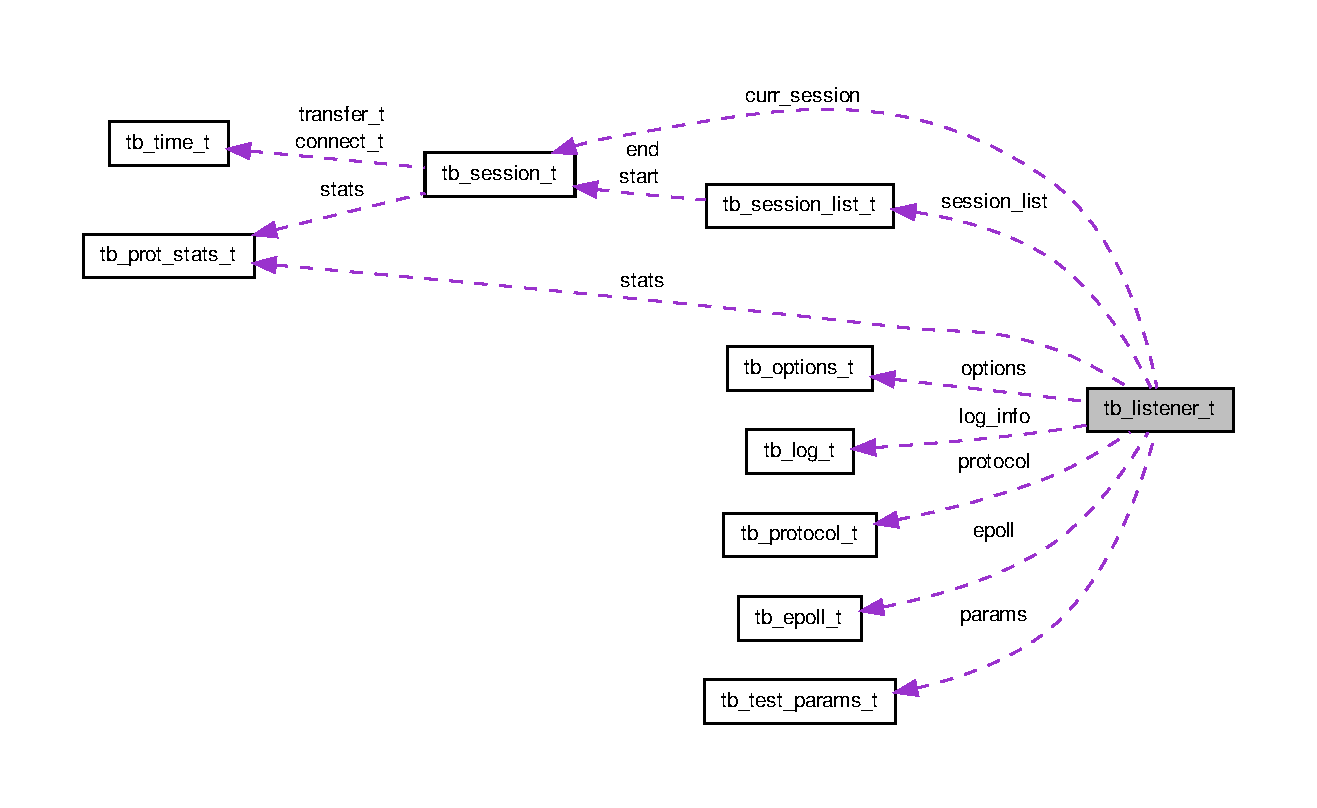
\includegraphics[width=350pt]{structtb__listener__t__coll__graph}
\end{center}
\end{figure}
\subsection*{Data Fields}
\begin{DoxyCompactItemize}
\item 
gdsl\-\_\-hash\-\_\-t \hyperlink{structtb__listener__t_a297b6218401cf4b88bf011d2665be0d2}{\-\_\-\-\_\-sessions}
\item 
gdsl\-\_\-heap\-\_\-t \hyperlink{structtb__listener__t_a41b2b73dc00fee2a18f90afa4987cc5b}{\-\_\-\-\_\-workers}
\begin{DoxyCompactList}\small\item\em The workers for this listener. \end{DoxyCompactList}\item 
int \hyperlink{structtb__listener__t_a49ffb28f94389b1ca495a663507db665}{\-\_\-\-\_\-num\-\_\-threads}
\begin{DoxyCompactList}\small\item\em The number of threads for listener. \end{DoxyCompactList}\item 
G\-Hash\-Table $\ast$ \hyperlink{structtb__listener__t_a696d2a3fd36c8895302b9372d1e55935}{sessions}
\begin{DoxyCompactList}\small\item\em Active sessions. \end{DoxyCompactList}\item 
pthread\-\_\-t $\ast$ \hyperlink{structtb__listener__t_a104cf2a79e8cb03fe3c0d3301fe8257f}{\-\_\-\-\_\-l\-\_\-thread}
\begin{DoxyCompactList}\small\item\em The thread the listener is on. \end{DoxyCompactList}\item 
int \hyperlink{structtb__listener__t_a053be2f9198a10c7329b11c19dfc6fe4}{sys\-\_\-tid}
\begin{DoxyCompactList}\small\item\em The id returned from syscall. \end{DoxyCompactList}\item 
pthread\-\_\-mutex\-\_\-t $\ast$ \hyperlink{structtb__listener__t_ab828bf6b1b85621025b518a892b79d79}{stat\-\_\-lock}
\begin{DoxyCompactList}\small\item\em Locks the stats field for writing. \end{DoxyCompactList}\item 
pthread\-\_\-cond\-\_\-t $\ast$ \hyperlink{structtb__listener__t_a7f764a9f865a1a752a852d4d4422023a}{stat\-\_\-cond}
\begin{DoxyCompactList}\small\item\em The condition for releasing external threads. \end{DoxyCompactList}\item 
pthread\-\_\-mutex\-\_\-t $\ast$ \hyperlink{structtb__listener__t_a54cc7a2ff1d7592de7c4647c6fd66e14}{status\-\_\-lock}
\begin{DoxyCompactList}\small\item\em Lock for safe set/get of listener status. \end{DoxyCompactList}\item 
int \hyperlink{structtb__listener__t_ae9a3e84ebf05ae6b7baf872b844c94ea}{num\-\_\-proc}
\begin{DoxyCompactList}\small\item\em The number of processors available. \end{DoxyCompactList}\item 
int \hyperlink{structtb__listener__t_ab7a892d2900125821f3d6b11d003191b}{cpu\-\_\-affinity}
\begin{DoxyCompactList}\small\item\em The affinity for the listener thread. \end{DoxyCompactList}\item 
int \hyperlink{structtb__listener__t_a2715f812fc8239e875c5e9413f8ed04b}{main\-\_\-cpu\-\_\-aff}
\begin{DoxyCompactList}\small\item\em The affinity for the main thread. \end{DoxyCompactList}\item 
\hyperlink{tb__listener_8h_ae37f3ebcf0081b2dd11adf41f1f867d6}{E\-N\-D\-P\-O\-I\-N\-T\-\_\-\-T\-Y\-P\-E} \hyperlink{structtb__listener__t_abbd1eee27b1b57dcb1f57b2ef4b4fa12}{e\-\_\-type}
\begin{DoxyCompactList}\small\item\em The type of endpoint this is. \end{DoxyCompactList}\item 
char $\ast$ \hyperlink{structtb__listener__t_ae15b37b2cdfd51bbb2719e4eb3ffb917}{bind\-\_\-address}
\begin{DoxyCompactList}\small\item\em The bind address for this listener. \end{DoxyCompactList}\item 
char $\ast$ \hyperlink{structtb__listener__t_a5c96fa09c995ca60f7b334c1842eb991}{bind\-\_\-port}
\begin{DoxyCompactList}\small\item\em The bind port for this listener. \end{DoxyCompactList}\item 
int \hyperlink{structtb__listener__t_a199ab88d4ca8eab30e1cb7d35edacca5}{bufsize}
\begin{DoxyCompactList}\small\item\em The size of the buffer to use. \end{DoxyCompactList}\item 
\hyperlink{structtb__protocol__t}{tb\-\_\-protocol\-\_\-t} $\ast$ \hyperlink{structtb__listener__t_a0b0f6789be37cb22fa42abe30a271591}{protocol}
\begin{DoxyCompactList}\small\item\em The protocol to use. \end{DoxyCompactList}\item 
int \hyperlink{structtb__listener__t_a94d540b145f21be2f9b28a2c225ccf30}{sock\-\_\-d}
\begin{DoxyCompactList}\small\item\em The socket descriptor. \end{DoxyCompactList}\item 
\hyperlink{structtb__options__t}{tb\-\_\-options\-\_\-t} $\ast$ \hyperlink{structtb__listener__t_abe6a138a14cade5eb871eeb66ee2b638}{options}
\begin{DoxyCompactList}\small\item\em The options for the protocol. \end{DoxyCompactList}\item 
void $\ast$ \hyperlink{structtb__listener__t_ab79822e20d19ce95bdf8a3f95bd616d5}{prot\-\_\-data}
\begin{DoxyCompactList}\small\item\em Protocol specific data. \end{DoxyCompactList}\item 
int \hyperlink{structtb__listener__t_acbf48788378975ac1fb514027e3dc1ab}{num\-\_\-connections}
\begin{DoxyCompactList}\small\item\em The number of connections to create;. \end{DoxyCompactList}\item 
int \hyperlink{structtb__listener__t_a8bc95708c758a6400d8692f2d0fcbaeb}{file\-\_\-size}
\begin{DoxyCompactList}\small\item\em The size of the file to generate. \end{DoxyCompactList}\item 
F\-I\-L\-E $\ast$ \hyperlink{structtb__listener__t_aa065f30aa9f5f9a42132c82c787ee70b}{fp}
\begin{DoxyCompactList}\small\item\em A pointer to the file to read/write to/from. \end{DoxyCompactList}\item 
char $\ast$ \hyperlink{structtb__listener__t_aeac90097f29f7529968697163cea5c18}{filename}
\begin{DoxyCompactList}\small\item\em The name of the file to load. \end{DoxyCompactList}\item 
char $\ast$ \hyperlink{structtb__listener__t_a91a70b77df95bd8b0830b49a094c2acb}{data}
\begin{DoxyCompactList}\small\item\em The data to send. \end{DoxyCompactList}\item 
int \hyperlink{structtb__listener__t_a875fd564b2b2de100e6fc2090a06812c}{num\-\_\-send}
\begin{DoxyCompactList}\small\item\em Send multiple times. \end{DoxyCompactList}\item 
struct addrinfo $\ast$ \hyperlink{structtb__listener__t_aab742bc33815bd69bf49ad1861006b97}{addr\-\_\-info}
\begin{DoxyCompactList}\small\item\em The addrinfo for the endpoint. \end{DoxyCompactList}\item 
int \hyperlink{structtb__listener__t_ac8bf36fe0577cba66bccda3a6f7e80a4}{flags}
\begin{DoxyCompactList}\small\item\em The flags for the endpoint. \end{DoxyCompactList}\item 
long long \hyperlink{structtb__listener__t_af6b56edb73bc2df2c5b45cb794532ce5}{total\-\_\-tx\-\_\-rx}
\begin{DoxyCompactList}\small\item\em the total amount of data tx/rx. \end{DoxyCompactList}\item 
double \hyperlink{structtb__listener__t_a741d9964fa8029b9468528756ea835af}{sec}
\begin{DoxyCompactList}\small\item\em The seconds it took for the last transfer. \end{DoxyCompactList}\item 
\hyperlink{structtb__prot__stats__t}{tb\-\_\-prot\-\_\-stats\-\_\-t} $\ast$ \hyperlink{structtb__listener__t_a464593aa6d4c80e0f689c501c4e81e8c}{stats}
\begin{DoxyCompactList}\small\item\em The current stats. \end{DoxyCompactList}\item 
int \hyperlink{structtb__listener__t_ad91878c8e805d88354749a9fbfee4296}{read}
\begin{DoxyCompactList}\small\item\em Current stats have been read. \end{DoxyCompactList}\item 
int \hyperlink{structtb__listener__t_a46fa1969de5714507943035793d36269}{monitor}
\begin{DoxyCompactList}\small\item\em Monitor for stat collection. \end{DoxyCompactList}\item 
int \hyperlink{structtb__listener__t_a21a0be842e8fa2c780fa87f45bd5d17e}{print\-\_\-stats}
\begin{DoxyCompactList}\small\item\em Print stats to screen. \end{DoxyCompactList}\item 
\hyperlink{tb__listener_8h_a32c27cc471df37f4fc818d65de0a56c4}{S\-T\-A\-T\-U\-S} \hyperlink{structtb__listener__t_a1025e6cbbd3179d2d91b9b4afb8f8efc}{status}
\begin{DoxyCompactList}\small\item\em The current status of the listener. \end{DoxyCompactList}\item 
\hyperlink{tb__listener_8h_a0fbada5bff0eeb4dc6be4b6e6f1c4eaf}{C\-O\-M\-M\-A\-N\-D} \hyperlink{structtb__listener__t_a70d431da3740b5dedad495c2843ba89e}{command}
\begin{DoxyCompactList}\small\item\em Commands to stop, etc. \end{DoxyCompactList}\item 
\hyperlink{tb__listener_8h_a0fbada5bff0eeb4dc6be4b6e6f1c4eaf}{C\-O\-M\-M\-A\-N\-D} \hyperlink{structtb__listener__t_aea40caaca885ba5ed3e0b82d7ef1f498}{s\-\_\-tx\-\_\-end}
\begin{DoxyCompactList}\small\item\em The command to process if a tx ends. \end{DoxyCompactList}\item 
int \hyperlink{structtb__listener__t_a73b88865af668ff87dacd74c1f838da6}{d\-\_\-exit}
\begin{DoxyCompactList}\small\item\em Destroy on exit. \end{DoxyCompactList}\item 
\hyperlink{structtb__test__params__t}{tb\-\_\-test\-\_\-params\-\_\-t} $\ast$ \hyperlink{structtb__listener__t_ada07b15315fdcc71589ed7b50faec50a}{params}
\begin{DoxyCompactList}\small\item\em The parameters for the test. \end{DoxyCompactList}\item 
int \hyperlink{structtb__listener__t_a511e73c6f56fe64b24f9261939aec65f}{log\-\_\-enabled}
\begin{DoxyCompactList}\small\item\em Logging enabled/disabled. \end{DoxyCompactList}\item 
\hyperlink{structtb__log__t}{tb\-\_\-log\-\_\-t} $\ast$ \hyperlink{structtb__listener__t_a206b8711b0b270577f073bdc99b0917d}{log\-\_\-info}
\begin{DoxyCompactList}\small\item\em Information for logging. \end{DoxyCompactList}\item 
\hyperlink{structtb__session__t}{tb\-\_\-session\-\_\-t} $\ast$ \hyperlink{structtb__listener__t_a77b5086c18c650adfe86a3489057d9f9}{curr\-\_\-session}
\item 
\hyperlink{structtb__epoll__t}{tb\-\_\-epoll\-\_\-t} $\ast$ \hyperlink{structtb__listener__t_af7fbbda1b15f6051fb8cead0ada5ce7e}{epoll}
\begin{DoxyCompactList}\small\item\em Used by protocols that require epoll;. \end{DoxyCompactList}\item 
\hyperlink{structtb__session__list__t}{tb\-\_\-session\-\_\-list\-\_\-t} $\ast$ \hyperlink{structtb__listener__t_a948f8e60166821d3db232c56a59b195c}{session\-\_\-list}
\begin{DoxyCompactList}\small\item\em Session list. \end{DoxyCompactList}\item 
\hyperlink{tb__listener_8h_a087aa7eae6394f6a052ea86a8944b262}{funct\-\_\-l\-\_\-exit} \hyperlink{structtb__listener__t_a90a87c6e5bc8d9e690190da6d0aa926e}{f\-\_\-exit}
\begin{DoxyCompactList}\small\item\em Called when aborting. \end{DoxyCompactList}\item 
\hyperlink{tb__listener_8h_a26990e2906e18234aa32e757383e1752}{funct\-\_\-l\-\_\-abort} \hyperlink{structtb__listener__t_a385e4cbcf683dd35d7d80c9726c8c67d}{f\-\_\-abort}
\begin{DoxyCompactList}\small\item\em Called when exiting. \end{DoxyCompactList}\end{DoxyCompactItemize}


\subsection{Detailed Description}
struct that defines the fields for the listener class. 

This is the 'main' struct used in testbed. It contains all of the data required to carry out a test. This information is set using command line parameters (when used as an application) or using the tb\-\_\-test\-\_\-param\-\_\-t struct, passed into the tb\-\_\-create\-\_\-endpoint function. 

Definition at line 140 of file tb\-\_\-listener.\-h.



\subsection{Field Documentation}
\hypertarget{structtb__listener__t_a104cf2a79e8cb03fe3c0d3301fe8257f}{\index{tb\-\_\-listener\-\_\-t@{tb\-\_\-listener\-\_\-t}!\-\_\-\-\_\-l\-\_\-thread@{\-\_\-\-\_\-l\-\_\-thread}}
\index{\-\_\-\-\_\-l\-\_\-thread@{\-\_\-\-\_\-l\-\_\-thread}!tb_listener_t@{tb\-\_\-listener\-\_\-t}}
\subsubsection[{\-\_\-\-\_\-l\-\_\-thread}]{\setlength{\rightskip}{0pt plus 5cm}pthread\-\_\-t$\ast$ \-\_\-\-\_\-l\-\_\-thread}}\label{structtb__listener__t_a104cf2a79e8cb03fe3c0d3301fe8257f}


The thread the listener is on. 



Definition at line 152 of file tb\-\_\-listener.\-h.

\hypertarget{structtb__listener__t_a49ffb28f94389b1ca495a663507db665}{\index{tb\-\_\-listener\-\_\-t@{tb\-\_\-listener\-\_\-t}!\-\_\-\-\_\-num\-\_\-threads@{\-\_\-\-\_\-num\-\_\-threads}}
\index{\-\_\-\-\_\-num\-\_\-threads@{\-\_\-\-\_\-num\-\_\-threads}!tb_listener_t@{tb\-\_\-listener\-\_\-t}}
\subsubsection[{\-\_\-\-\_\-num\-\_\-threads}]{\setlength{\rightskip}{0pt plus 5cm}int \-\_\-\-\_\-num\-\_\-threads}}\label{structtb__listener__t_a49ffb28f94389b1ca495a663507db665}


The number of threads for listener. 



Definition at line 148 of file tb\-\_\-listener.\-h.

\hypertarget{structtb__listener__t_a297b6218401cf4b88bf011d2665be0d2}{\index{tb\-\_\-listener\-\_\-t@{tb\-\_\-listener\-\_\-t}!\-\_\-\-\_\-sessions@{\-\_\-\-\_\-sessions}}
\index{\-\_\-\-\_\-sessions@{\-\_\-\-\_\-sessions}!tb_listener_t@{tb\-\_\-listener\-\_\-t}}
\subsubsection[{\-\_\-\-\_\-sessions}]{\setlength{\rightskip}{0pt plus 5cm}gdsl\-\_\-hash\-\_\-t \-\_\-\-\_\-sessions}}\label{structtb__listener__t_a297b6218401cf4b88bf011d2665be0d2}
The active sessions for this listener. Maps address to listener. 

Definition at line 143 of file tb\-\_\-listener.\-h.

\hypertarget{structtb__listener__t_a41b2b73dc00fee2a18f90afa4987cc5b}{\index{tb\-\_\-listener\-\_\-t@{tb\-\_\-listener\-\_\-t}!\-\_\-\-\_\-workers@{\-\_\-\-\_\-workers}}
\index{\-\_\-\-\_\-workers@{\-\_\-\-\_\-workers}!tb_listener_t@{tb\-\_\-listener\-\_\-t}}
\subsubsection[{\-\_\-\-\_\-workers}]{\setlength{\rightskip}{0pt plus 5cm}gdsl\-\_\-heap\-\_\-t \-\_\-\-\_\-workers}}\label{structtb__listener__t_a41b2b73dc00fee2a18f90afa4987cc5b}


The workers for this listener. 



Definition at line 147 of file tb\-\_\-listener.\-h.

\hypertarget{structtb__listener__t_aab742bc33815bd69bf49ad1861006b97}{\index{tb\-\_\-listener\-\_\-t@{tb\-\_\-listener\-\_\-t}!addr\-\_\-info@{addr\-\_\-info}}
\index{addr\-\_\-info@{addr\-\_\-info}!tb_listener_t@{tb\-\_\-listener\-\_\-t}}
\subsubsection[{addr\-\_\-info}]{\setlength{\rightskip}{0pt plus 5cm}struct addrinfo$\ast$ addr\-\_\-info}}\label{structtb__listener__t_aab742bc33815bd69bf49ad1861006b97}


The addrinfo for the endpoint. 



Definition at line 183 of file tb\-\_\-listener.\-h.

\hypertarget{structtb__listener__t_ae15b37b2cdfd51bbb2719e4eb3ffb917}{\index{tb\-\_\-listener\-\_\-t@{tb\-\_\-listener\-\_\-t}!bind\-\_\-address@{bind\-\_\-address}}
\index{bind\-\_\-address@{bind\-\_\-address}!tb_listener_t@{tb\-\_\-listener\-\_\-t}}
\subsubsection[{bind\-\_\-address}]{\setlength{\rightskip}{0pt plus 5cm}char$\ast$ bind\-\_\-address}}\label{structtb__listener__t_ae15b37b2cdfd51bbb2719e4eb3ffb917}


The bind address for this listener. 



Definition at line 167 of file tb\-\_\-listener.\-h.

\hypertarget{structtb__listener__t_a5c96fa09c995ca60f7b334c1842eb991}{\index{tb\-\_\-listener\-\_\-t@{tb\-\_\-listener\-\_\-t}!bind\-\_\-port@{bind\-\_\-port}}
\index{bind\-\_\-port@{bind\-\_\-port}!tb_listener_t@{tb\-\_\-listener\-\_\-t}}
\subsubsection[{bind\-\_\-port}]{\setlength{\rightskip}{0pt plus 5cm}char$\ast$ bind\-\_\-port}}\label{structtb__listener__t_a5c96fa09c995ca60f7b334c1842eb991}


The bind port for this listener. 



Definition at line 168 of file tb\-\_\-listener.\-h.

\hypertarget{structtb__listener__t_a199ab88d4ca8eab30e1cb7d35edacca5}{\index{tb\-\_\-listener\-\_\-t@{tb\-\_\-listener\-\_\-t}!bufsize@{bufsize}}
\index{bufsize@{bufsize}!tb_listener_t@{tb\-\_\-listener\-\_\-t}}
\subsubsection[{bufsize}]{\setlength{\rightskip}{0pt plus 5cm}int bufsize}}\label{structtb__listener__t_a199ab88d4ca8eab30e1cb7d35edacca5}


The size of the buffer to use. 



Definition at line 169 of file tb\-\_\-listener.\-h.

\hypertarget{structtb__listener__t_a70d431da3740b5dedad495c2843ba89e}{\index{tb\-\_\-listener\-\_\-t@{tb\-\_\-listener\-\_\-t}!command@{command}}
\index{command@{command}!tb_listener_t@{tb\-\_\-listener\-\_\-t}}
\subsubsection[{command}]{\setlength{\rightskip}{0pt plus 5cm}{\bf C\-O\-M\-M\-A\-N\-D} command}}\label{structtb__listener__t_a70d431da3740b5dedad495c2843ba89e}


Commands to stop, etc. 



Definition at line 199 of file tb\-\_\-listener.\-h.

\hypertarget{structtb__listener__t_ab7a892d2900125821f3d6b11d003191b}{\index{tb\-\_\-listener\-\_\-t@{tb\-\_\-listener\-\_\-t}!cpu\-\_\-affinity@{cpu\-\_\-affinity}}
\index{cpu\-\_\-affinity@{cpu\-\_\-affinity}!tb_listener_t@{tb\-\_\-listener\-\_\-t}}
\subsubsection[{cpu\-\_\-affinity}]{\setlength{\rightskip}{0pt plus 5cm}int cpu\-\_\-affinity}}\label{structtb__listener__t_ab7a892d2900125821f3d6b11d003191b}


The affinity for the listener thread. 



Definition at line 160 of file tb\-\_\-listener.\-h.

\hypertarget{structtb__listener__t_a77b5086c18c650adfe86a3489057d9f9}{\index{tb\-\_\-listener\-\_\-t@{tb\-\_\-listener\-\_\-t}!curr\-\_\-session@{curr\-\_\-session}}
\index{curr\-\_\-session@{curr\-\_\-session}!tb_listener_t@{tb\-\_\-listener\-\_\-t}}
\subsubsection[{curr\-\_\-session}]{\setlength{\rightskip}{0pt plus 5cm}{\bf tb\-\_\-session\-\_\-t}$\ast$ curr\-\_\-session}}\label{structtb__listener__t_a77b5086c18c650adfe86a3489057d9f9}


Definition at line 211 of file tb\-\_\-listener.\-h.

\hypertarget{structtb__listener__t_a73b88865af668ff87dacd74c1f838da6}{\index{tb\-\_\-listener\-\_\-t@{tb\-\_\-listener\-\_\-t}!d\-\_\-exit@{d\-\_\-exit}}
\index{d\-\_\-exit@{d\-\_\-exit}!tb_listener_t@{tb\-\_\-listener\-\_\-t}}
\subsubsection[{d\-\_\-exit}]{\setlength{\rightskip}{0pt plus 5cm}int d\-\_\-exit}}\label{structtb__listener__t_a73b88865af668ff87dacd74c1f838da6}


Destroy on exit. 



Definition at line 201 of file tb\-\_\-listener.\-h.

\hypertarget{structtb__listener__t_a91a70b77df95bd8b0830b49a094c2acb}{\index{tb\-\_\-listener\-\_\-t@{tb\-\_\-listener\-\_\-t}!data@{data}}
\index{data@{data}!tb_listener_t@{tb\-\_\-listener\-\_\-t}}
\subsubsection[{data}]{\setlength{\rightskip}{0pt plus 5cm}char$\ast$ data}}\label{structtb__listener__t_a91a70b77df95bd8b0830b49a094c2acb}


The data to send. 



Definition at line 180 of file tb\-\_\-listener.\-h.

\hypertarget{structtb__listener__t_abbd1eee27b1b57dcb1f57b2ef4b4fa12}{\index{tb\-\_\-listener\-\_\-t@{tb\-\_\-listener\-\_\-t}!e\-\_\-type@{e\-\_\-type}}
\index{e\-\_\-type@{e\-\_\-type}!tb_listener_t@{tb\-\_\-listener\-\_\-t}}
\subsubsection[{e\-\_\-type}]{\setlength{\rightskip}{0pt plus 5cm}{\bf E\-N\-D\-P\-O\-I\-N\-T\-\_\-\-T\-Y\-P\-E} e\-\_\-type}}\label{structtb__listener__t_abbd1eee27b1b57dcb1f57b2ef4b4fa12}


The type of endpoint this is. 



Definition at line 164 of file tb\-\_\-listener.\-h.

\hypertarget{structtb__listener__t_af7fbbda1b15f6051fb8cead0ada5ce7e}{\index{tb\-\_\-listener\-\_\-t@{tb\-\_\-listener\-\_\-t}!epoll@{epoll}}
\index{epoll@{epoll}!tb_listener_t@{tb\-\_\-listener\-\_\-t}}
\subsubsection[{epoll}]{\setlength{\rightskip}{0pt plus 5cm}{\bf tb\-\_\-epoll\-\_\-t}$\ast$ epoll}}\label{structtb__listener__t_af7fbbda1b15f6051fb8cead0ada5ce7e}


Used by protocols that require epoll;. 



Definition at line 212 of file tb\-\_\-listener.\-h.

\hypertarget{structtb__listener__t_a385e4cbcf683dd35d7d80c9726c8c67d}{\index{tb\-\_\-listener\-\_\-t@{tb\-\_\-listener\-\_\-t}!f\-\_\-abort@{f\-\_\-abort}}
\index{f\-\_\-abort@{f\-\_\-abort}!tb_listener_t@{tb\-\_\-listener\-\_\-t}}
\subsubsection[{f\-\_\-abort}]{\setlength{\rightskip}{0pt plus 5cm}{\bf funct\-\_\-l\-\_\-abort} f\-\_\-abort}}\label{structtb__listener__t_a385e4cbcf683dd35d7d80c9726c8c67d}


Called when exiting. 



Definition at line 217 of file tb\-\_\-listener.\-h.

\hypertarget{structtb__listener__t_a90a87c6e5bc8d9e690190da6d0aa926e}{\index{tb\-\_\-listener\-\_\-t@{tb\-\_\-listener\-\_\-t}!f\-\_\-exit@{f\-\_\-exit}}
\index{f\-\_\-exit@{f\-\_\-exit}!tb_listener_t@{tb\-\_\-listener\-\_\-t}}
\subsubsection[{f\-\_\-exit}]{\setlength{\rightskip}{0pt plus 5cm}{\bf funct\-\_\-l\-\_\-exit} f\-\_\-exit}}\label{structtb__listener__t_a90a87c6e5bc8d9e690190da6d0aa926e}


Called when aborting. 



Definition at line 216 of file tb\-\_\-listener.\-h.

\hypertarget{structtb__listener__t_a8bc95708c758a6400d8692f2d0fcbaeb}{\index{tb\-\_\-listener\-\_\-t@{tb\-\_\-listener\-\_\-t}!file\-\_\-size@{file\-\_\-size}}
\index{file\-\_\-size@{file\-\_\-size}!tb_listener_t@{tb\-\_\-listener\-\_\-t}}
\subsubsection[{file\-\_\-size}]{\setlength{\rightskip}{0pt plus 5cm}int file\-\_\-size}}\label{structtb__listener__t_a8bc95708c758a6400d8692f2d0fcbaeb}


The size of the file to generate. 



Definition at line 177 of file tb\-\_\-listener.\-h.

\hypertarget{structtb__listener__t_aeac90097f29f7529968697163cea5c18}{\index{tb\-\_\-listener\-\_\-t@{tb\-\_\-listener\-\_\-t}!filename@{filename}}
\index{filename@{filename}!tb_listener_t@{tb\-\_\-listener\-\_\-t}}
\subsubsection[{filename}]{\setlength{\rightskip}{0pt plus 5cm}char$\ast$ filename}}\label{structtb__listener__t_aeac90097f29f7529968697163cea5c18}


The name of the file to load. 



Definition at line 179 of file tb\-\_\-listener.\-h.

\hypertarget{structtb__listener__t_ac8bf36fe0577cba66bccda3a6f7e80a4}{\index{tb\-\_\-listener\-\_\-t@{tb\-\_\-listener\-\_\-t}!flags@{flags}}
\index{flags@{flags}!tb_listener_t@{tb\-\_\-listener\-\_\-t}}
\subsubsection[{flags}]{\setlength{\rightskip}{0pt plus 5cm}int flags}}\label{structtb__listener__t_ac8bf36fe0577cba66bccda3a6f7e80a4}


The flags for the endpoint. 



Definition at line 184 of file tb\-\_\-listener.\-h.

\hypertarget{structtb__listener__t_aa065f30aa9f5f9a42132c82c787ee70b}{\index{tb\-\_\-listener\-\_\-t@{tb\-\_\-listener\-\_\-t}!fp@{fp}}
\index{fp@{fp}!tb_listener_t@{tb\-\_\-listener\-\_\-t}}
\subsubsection[{fp}]{\setlength{\rightskip}{0pt plus 5cm}F\-I\-L\-E$\ast$ fp}}\label{structtb__listener__t_aa065f30aa9f5f9a42132c82c787ee70b}


A pointer to the file to read/write to/from. 



Definition at line 178 of file tb\-\_\-listener.\-h.

\hypertarget{structtb__listener__t_a511e73c6f56fe64b24f9261939aec65f}{\index{tb\-\_\-listener\-\_\-t@{tb\-\_\-listener\-\_\-t}!log\-\_\-enabled@{log\-\_\-enabled}}
\index{log\-\_\-enabled@{log\-\_\-enabled}!tb_listener_t@{tb\-\_\-listener\-\_\-t}}
\subsubsection[{log\-\_\-enabled}]{\setlength{\rightskip}{0pt plus 5cm}int log\-\_\-enabled}}\label{structtb__listener__t_a511e73c6f56fe64b24f9261939aec65f}


Logging enabled/disabled. 



Definition at line 207 of file tb\-\_\-listener.\-h.

\hypertarget{structtb__listener__t_a206b8711b0b270577f073bdc99b0917d}{\index{tb\-\_\-listener\-\_\-t@{tb\-\_\-listener\-\_\-t}!log\-\_\-info@{log\-\_\-info}}
\index{log\-\_\-info@{log\-\_\-info}!tb_listener_t@{tb\-\_\-listener\-\_\-t}}
\subsubsection[{log\-\_\-info}]{\setlength{\rightskip}{0pt plus 5cm}{\bf tb\-\_\-log\-\_\-t}$\ast$ log\-\_\-info}}\label{structtb__listener__t_a206b8711b0b270577f073bdc99b0917d}


Information for logging. 



Definition at line 208 of file tb\-\_\-listener.\-h.

\hypertarget{structtb__listener__t_a2715f812fc8239e875c5e9413f8ed04b}{\index{tb\-\_\-listener\-\_\-t@{tb\-\_\-listener\-\_\-t}!main\-\_\-cpu\-\_\-aff@{main\-\_\-cpu\-\_\-aff}}
\index{main\-\_\-cpu\-\_\-aff@{main\-\_\-cpu\-\_\-aff}!tb_listener_t@{tb\-\_\-listener\-\_\-t}}
\subsubsection[{main\-\_\-cpu\-\_\-aff}]{\setlength{\rightskip}{0pt plus 5cm}int main\-\_\-cpu\-\_\-aff}}\label{structtb__listener__t_a2715f812fc8239e875c5e9413f8ed04b}


The affinity for the main thread. 



Definition at line 161 of file tb\-\_\-listener.\-h.

\hypertarget{structtb__listener__t_a46fa1969de5714507943035793d36269}{\index{tb\-\_\-listener\-\_\-t@{tb\-\_\-listener\-\_\-t}!monitor@{monitor}}
\index{monitor@{monitor}!tb_listener_t@{tb\-\_\-listener\-\_\-t}}
\subsubsection[{monitor}]{\setlength{\rightskip}{0pt plus 5cm}int monitor}}\label{structtb__listener__t_a46fa1969de5714507943035793d36269}


Monitor for stat collection. 



Definition at line 194 of file tb\-\_\-listener.\-h.

\hypertarget{structtb__listener__t_acbf48788378975ac1fb514027e3dc1ab}{\index{tb\-\_\-listener\-\_\-t@{tb\-\_\-listener\-\_\-t}!num\-\_\-connections@{num\-\_\-connections}}
\index{num\-\_\-connections@{num\-\_\-connections}!tb_listener_t@{tb\-\_\-listener\-\_\-t}}
\subsubsection[{num\-\_\-connections}]{\setlength{\rightskip}{0pt plus 5cm}int num\-\_\-connections}}\label{structtb__listener__t_acbf48788378975ac1fb514027e3dc1ab}


The number of connections to create;. 



Definition at line 174 of file tb\-\_\-listener.\-h.

\hypertarget{structtb__listener__t_ae9a3e84ebf05ae6b7baf872b844c94ea}{\index{tb\-\_\-listener\-\_\-t@{tb\-\_\-listener\-\_\-t}!num\-\_\-proc@{num\-\_\-proc}}
\index{num\-\_\-proc@{num\-\_\-proc}!tb_listener_t@{tb\-\_\-listener\-\_\-t}}
\subsubsection[{num\-\_\-proc}]{\setlength{\rightskip}{0pt plus 5cm}int num\-\_\-proc}}\label{structtb__listener__t_ae9a3e84ebf05ae6b7baf872b844c94ea}


The number of processors available. 



Definition at line 159 of file tb\-\_\-listener.\-h.

\hypertarget{structtb__listener__t_a875fd564b2b2de100e6fc2090a06812c}{\index{tb\-\_\-listener\-\_\-t@{tb\-\_\-listener\-\_\-t}!num\-\_\-send@{num\-\_\-send}}
\index{num\-\_\-send@{num\-\_\-send}!tb_listener_t@{tb\-\_\-listener\-\_\-t}}
\subsubsection[{num\-\_\-send}]{\setlength{\rightskip}{0pt plus 5cm}int num\-\_\-send}}\label{structtb__listener__t_a875fd564b2b2de100e6fc2090a06812c}


Send multiple times. 



Definition at line 181 of file tb\-\_\-listener.\-h.

\hypertarget{structtb__listener__t_abe6a138a14cade5eb871eeb66ee2b638}{\index{tb\-\_\-listener\-\_\-t@{tb\-\_\-listener\-\_\-t}!options@{options}}
\index{options@{options}!tb_listener_t@{tb\-\_\-listener\-\_\-t}}
\subsubsection[{options}]{\setlength{\rightskip}{0pt plus 5cm}{\bf tb\-\_\-options\-\_\-t}$\ast$ options}}\label{structtb__listener__t_abe6a138a14cade5eb871eeb66ee2b638}


The options for the protocol. 



Definition at line 172 of file tb\-\_\-listener.\-h.

\hypertarget{structtb__listener__t_ada07b15315fdcc71589ed7b50faec50a}{\index{tb\-\_\-listener\-\_\-t@{tb\-\_\-listener\-\_\-t}!params@{params}}
\index{params@{params}!tb_listener_t@{tb\-\_\-listener\-\_\-t}}
\subsubsection[{params}]{\setlength{\rightskip}{0pt plus 5cm}{\bf tb\-\_\-test\-\_\-params\-\_\-t}$\ast$ params}}\label{structtb__listener__t_ada07b15315fdcc71589ed7b50faec50a}


The parameters for the test. 



Definition at line 204 of file tb\-\_\-listener.\-h.

\hypertarget{structtb__listener__t_a21a0be842e8fa2c780fa87f45bd5d17e}{\index{tb\-\_\-listener\-\_\-t@{tb\-\_\-listener\-\_\-t}!print\-\_\-stats@{print\-\_\-stats}}
\index{print\-\_\-stats@{print\-\_\-stats}!tb_listener_t@{tb\-\_\-listener\-\_\-t}}
\subsubsection[{print\-\_\-stats}]{\setlength{\rightskip}{0pt plus 5cm}int print\-\_\-stats}}\label{structtb__listener__t_a21a0be842e8fa2c780fa87f45bd5d17e}


Print stats to screen. 



Definition at line 195 of file tb\-\_\-listener.\-h.

\hypertarget{structtb__listener__t_ab79822e20d19ce95bdf8a3f95bd616d5}{\index{tb\-\_\-listener\-\_\-t@{tb\-\_\-listener\-\_\-t}!prot\-\_\-data@{prot\-\_\-data}}
\index{prot\-\_\-data@{prot\-\_\-data}!tb_listener_t@{tb\-\_\-listener\-\_\-t}}
\subsubsection[{prot\-\_\-data}]{\setlength{\rightskip}{0pt plus 5cm}void$\ast$ prot\-\_\-data}}\label{structtb__listener__t_ab79822e20d19ce95bdf8a3f95bd616d5}


Protocol specific data. 



Definition at line 173 of file tb\-\_\-listener.\-h.

\hypertarget{structtb__listener__t_a0b0f6789be37cb22fa42abe30a271591}{\index{tb\-\_\-listener\-\_\-t@{tb\-\_\-listener\-\_\-t}!protocol@{protocol}}
\index{protocol@{protocol}!tb_listener_t@{tb\-\_\-listener\-\_\-t}}
\subsubsection[{protocol}]{\setlength{\rightskip}{0pt plus 5cm}{\bf tb\-\_\-protocol\-\_\-t}$\ast$ protocol}}\label{structtb__listener__t_a0b0f6789be37cb22fa42abe30a271591}


The protocol to use. 



Definition at line 170 of file tb\-\_\-listener.\-h.

\hypertarget{structtb__listener__t_ad91878c8e805d88354749a9fbfee4296}{\index{tb\-\_\-listener\-\_\-t@{tb\-\_\-listener\-\_\-t}!read@{read}}
\index{read@{read}!tb_listener_t@{tb\-\_\-listener\-\_\-t}}
\subsubsection[{read}]{\setlength{\rightskip}{0pt plus 5cm}int read}}\label{structtb__listener__t_ad91878c8e805d88354749a9fbfee4296}


Current stats have been read. 



Definition at line 193 of file tb\-\_\-listener.\-h.

\hypertarget{structtb__listener__t_aea40caaca885ba5ed3e0b82d7ef1f498}{\index{tb\-\_\-listener\-\_\-t@{tb\-\_\-listener\-\_\-t}!s\-\_\-tx\-\_\-end@{s\-\_\-tx\-\_\-end}}
\index{s\-\_\-tx\-\_\-end@{s\-\_\-tx\-\_\-end}!tb_listener_t@{tb\-\_\-listener\-\_\-t}}
\subsubsection[{s\-\_\-tx\-\_\-end}]{\setlength{\rightskip}{0pt plus 5cm}{\bf C\-O\-M\-M\-A\-N\-D} s\-\_\-tx\-\_\-end}}\label{structtb__listener__t_aea40caaca885ba5ed3e0b82d7ef1f498}


The command to process if a tx ends. 



Definition at line 200 of file tb\-\_\-listener.\-h.

\hypertarget{structtb__listener__t_a741d9964fa8029b9468528756ea835af}{\index{tb\-\_\-listener\-\_\-t@{tb\-\_\-listener\-\_\-t}!sec@{sec}}
\index{sec@{sec}!tb_listener_t@{tb\-\_\-listener\-\_\-t}}
\subsubsection[{sec}]{\setlength{\rightskip}{0pt plus 5cm}double sec}}\label{structtb__listener__t_a741d9964fa8029b9468528756ea835af}


The seconds it took for the last transfer. 



Definition at line 189 of file tb\-\_\-listener.\-h.

\hypertarget{structtb__listener__t_a948f8e60166821d3db232c56a59b195c}{\index{tb\-\_\-listener\-\_\-t@{tb\-\_\-listener\-\_\-t}!session\-\_\-list@{session\-\_\-list}}
\index{session\-\_\-list@{session\-\_\-list}!tb_listener_t@{tb\-\_\-listener\-\_\-t}}
\subsubsection[{session\-\_\-list}]{\setlength{\rightskip}{0pt plus 5cm}{\bf tb\-\_\-session\-\_\-list\-\_\-t}$\ast$ session\-\_\-list}}\label{structtb__listener__t_a948f8e60166821d3db232c56a59b195c}


Session list. 



Definition at line 213 of file tb\-\_\-listener.\-h.

\hypertarget{structtb__listener__t_a696d2a3fd36c8895302b9372d1e55935}{\index{tb\-\_\-listener\-\_\-t@{tb\-\_\-listener\-\_\-t}!sessions@{sessions}}
\index{sessions@{sessions}!tb_listener_t@{tb\-\_\-listener\-\_\-t}}
\subsubsection[{sessions}]{\setlength{\rightskip}{0pt plus 5cm}G\-Hash\-Table$\ast$ sessions}}\label{structtb__listener__t_a696d2a3fd36c8895302b9372d1e55935}


Active sessions. 



Definition at line 150 of file tb\-\_\-listener.\-h.

\hypertarget{structtb__listener__t_a94d540b145f21be2f9b28a2c225ccf30}{\index{tb\-\_\-listener\-\_\-t@{tb\-\_\-listener\-\_\-t}!sock\-\_\-d@{sock\-\_\-d}}
\index{sock\-\_\-d@{sock\-\_\-d}!tb_listener_t@{tb\-\_\-listener\-\_\-t}}
\subsubsection[{sock\-\_\-d}]{\setlength{\rightskip}{0pt plus 5cm}int sock\-\_\-d}}\label{structtb__listener__t_a94d540b145f21be2f9b28a2c225ccf30}


The socket descriptor. 



Definition at line 171 of file tb\-\_\-listener.\-h.

\hypertarget{structtb__listener__t_a7f764a9f865a1a752a852d4d4422023a}{\index{tb\-\_\-listener\-\_\-t@{tb\-\_\-listener\-\_\-t}!stat\-\_\-cond@{stat\-\_\-cond}}
\index{stat\-\_\-cond@{stat\-\_\-cond}!tb_listener_t@{tb\-\_\-listener\-\_\-t}}
\subsubsection[{stat\-\_\-cond}]{\setlength{\rightskip}{0pt plus 5cm}pthread\-\_\-cond\-\_\-t$\ast$ stat\-\_\-cond}}\label{structtb__listener__t_a7f764a9f865a1a752a852d4d4422023a}


The condition for releasing external threads. 



Definition at line 155 of file tb\-\_\-listener.\-h.

\hypertarget{structtb__listener__t_ab828bf6b1b85621025b518a892b79d79}{\index{tb\-\_\-listener\-\_\-t@{tb\-\_\-listener\-\_\-t}!stat\-\_\-lock@{stat\-\_\-lock}}
\index{stat\-\_\-lock@{stat\-\_\-lock}!tb_listener_t@{tb\-\_\-listener\-\_\-t}}
\subsubsection[{stat\-\_\-lock}]{\setlength{\rightskip}{0pt plus 5cm}pthread\-\_\-mutex\-\_\-t$\ast$ stat\-\_\-lock}}\label{structtb__listener__t_ab828bf6b1b85621025b518a892b79d79}


Locks the stats field for writing. 



Definition at line 154 of file tb\-\_\-listener.\-h.

\hypertarget{structtb__listener__t_a464593aa6d4c80e0f689c501c4e81e8c}{\index{tb\-\_\-listener\-\_\-t@{tb\-\_\-listener\-\_\-t}!stats@{stats}}
\index{stats@{stats}!tb_listener_t@{tb\-\_\-listener\-\_\-t}}
\subsubsection[{stats}]{\setlength{\rightskip}{0pt plus 5cm}{\bf tb\-\_\-prot\-\_\-stats\-\_\-t}$\ast$ stats}}\label{structtb__listener__t_a464593aa6d4c80e0f689c501c4e81e8c}


The current stats. 



Definition at line 192 of file tb\-\_\-listener.\-h.

\hypertarget{structtb__listener__t_a1025e6cbbd3179d2d91b9b4afb8f8efc}{\index{tb\-\_\-listener\-\_\-t@{tb\-\_\-listener\-\_\-t}!status@{status}}
\index{status@{status}!tb_listener_t@{tb\-\_\-listener\-\_\-t}}
\subsubsection[{status}]{\setlength{\rightskip}{0pt plus 5cm}{\bf S\-T\-A\-T\-U\-S} status}}\label{structtb__listener__t_a1025e6cbbd3179d2d91b9b4afb8f8efc}


The current status of the listener. 



Definition at line 198 of file tb\-\_\-listener.\-h.

\hypertarget{structtb__listener__t_a54cc7a2ff1d7592de7c4647c6fd66e14}{\index{tb\-\_\-listener\-\_\-t@{tb\-\_\-listener\-\_\-t}!status\-\_\-lock@{status\-\_\-lock}}
\index{status\-\_\-lock@{status\-\_\-lock}!tb_listener_t@{tb\-\_\-listener\-\_\-t}}
\subsubsection[{status\-\_\-lock}]{\setlength{\rightskip}{0pt plus 5cm}pthread\-\_\-mutex\-\_\-t$\ast$ status\-\_\-lock}}\label{structtb__listener__t_a54cc7a2ff1d7592de7c4647c6fd66e14}


Lock for safe set/get of listener status. 



Definition at line 156 of file tb\-\_\-listener.\-h.

\hypertarget{structtb__listener__t_a053be2f9198a10c7329b11c19dfc6fe4}{\index{tb\-\_\-listener\-\_\-t@{tb\-\_\-listener\-\_\-t}!sys\-\_\-tid@{sys\-\_\-tid}}
\index{sys\-\_\-tid@{sys\-\_\-tid}!tb_listener_t@{tb\-\_\-listener\-\_\-t}}
\subsubsection[{sys\-\_\-tid}]{\setlength{\rightskip}{0pt plus 5cm}int sys\-\_\-tid}}\label{structtb__listener__t_a053be2f9198a10c7329b11c19dfc6fe4}


The id returned from syscall. 



Definition at line 153 of file tb\-\_\-listener.\-h.

\hypertarget{structtb__listener__t_af6b56edb73bc2df2c5b45cb794532ce5}{\index{tb\-\_\-listener\-\_\-t@{tb\-\_\-listener\-\_\-t}!total\-\_\-tx\-\_\-rx@{total\-\_\-tx\-\_\-rx}}
\index{total\-\_\-tx\-\_\-rx@{total\-\_\-tx\-\_\-rx}!tb_listener_t@{tb\-\_\-listener\-\_\-t}}
\subsubsection[{total\-\_\-tx\-\_\-rx}]{\setlength{\rightskip}{0pt plus 5cm}long long total\-\_\-tx\-\_\-rx}}\label{structtb__listener__t_af6b56edb73bc2df2c5b45cb794532ce5}


the total amount of data tx/rx. 



Definition at line 188 of file tb\-\_\-listener.\-h.



The documentation for this struct was generated from the following file\-:\begin{DoxyCompactItemize}
\item 
src/\hyperlink{tb__listener_8h}{tb\-\_\-listener.\-h}\end{DoxyCompactItemize}

\hypertarget{structtb__log__t}{\section{tb\-\_\-log\-\_\-t Struct Reference}
\label{structtb__log__t}\index{tb\-\_\-log\-\_\-t@{tb\-\_\-log\-\_\-t}}
}


{\ttfamily \#include $<$tb\-\_\-logging.\-h$>$}

\subsection*{Data Fields}
\begin{DoxyCompactItemize}
\item 
F\-I\-L\-E $\ast$ \hyperlink{structtb__log__t_a702945180aa732857b380a007a7e2a21}{file}
\item 
char $\ast$ \hyperlink{structtb__log__t_a19064fd51f3a2b4b3c6e8ac8c09850c2}{file\-\_\-path}
\item 
int \hyperlink{structtb__log__t_a40c07165efeb9ce3aff7ce4c4d02af26}{file\-\_\-len}
\end{DoxyCompactItemize}


\subsection{Detailed Description}


Definition at line 17 of file tb\-\_\-logging.\-h.



\subsection{Field Documentation}
\hypertarget{structtb__log__t_a702945180aa732857b380a007a7e2a21}{\index{tb\-\_\-log\-\_\-t@{tb\-\_\-log\-\_\-t}!file@{file}}
\index{file@{file}!tb_log_t@{tb\-\_\-log\-\_\-t}}
\subsubsection[{file}]{\setlength{\rightskip}{0pt plus 5cm}F\-I\-L\-E$\ast$ file}}\label{structtb__log__t_a702945180aa732857b380a007a7e2a21}


Definition at line 19 of file tb\-\_\-logging.\-h.

\hypertarget{structtb__log__t_a40c07165efeb9ce3aff7ce4c4d02af26}{\index{tb\-\_\-log\-\_\-t@{tb\-\_\-log\-\_\-t}!file\-\_\-len@{file\-\_\-len}}
\index{file\-\_\-len@{file\-\_\-len}!tb_log_t@{tb\-\_\-log\-\_\-t}}
\subsubsection[{file\-\_\-len}]{\setlength{\rightskip}{0pt plus 5cm}int file\-\_\-len}}\label{structtb__log__t_a40c07165efeb9ce3aff7ce4c4d02af26}


Definition at line 21 of file tb\-\_\-logging.\-h.

\hypertarget{structtb__log__t_a19064fd51f3a2b4b3c6e8ac8c09850c2}{\index{tb\-\_\-log\-\_\-t@{tb\-\_\-log\-\_\-t}!file\-\_\-path@{file\-\_\-path}}
\index{file\-\_\-path@{file\-\_\-path}!tb_log_t@{tb\-\_\-log\-\_\-t}}
\subsubsection[{file\-\_\-path}]{\setlength{\rightskip}{0pt plus 5cm}char$\ast$ file\-\_\-path}}\label{structtb__log__t_a19064fd51f3a2b4b3c6e8ac8c09850c2}


Definition at line 20 of file tb\-\_\-logging.\-h.



The documentation for this struct was generated from the following file\-:\begin{DoxyCompactItemize}
\item 
src/\hyperlink{tb__logging_8h}{tb\-\_\-logging.\-h}\end{DoxyCompactItemize}

\hypertarget{structtb__options__t}{\section{tb\-\_\-options\-\_\-t Struct Reference}
\label{structtb__options__t}\index{tb\-\_\-options\-\_\-t@{tb\-\_\-options\-\_\-t}}
}


{\ttfamily \#include $<$tb\-\_\-sock\-\_\-opt.\-h$>$}

\subsection*{Data Fields}
\begin{DoxyCompactItemize}
\item 
\hyperlink{tb__protocol_8h_a7a5bff1040fc154c510874327d44cc1a}{P\-R\-O\-T\-O\-C\-O\-L} \hyperlink{structtb__options__t_a0d2276cd987e688180eedab183cd503e}{protocol}
\begin{DoxyCompactList}\small\item\em The protocol for these options. \end{DoxyCompactList}\item 
int \hyperlink{structtb__options__t_a8ae9ae9a85fbb77bc460b0d43e4fc1c5}{l4\-\_\-r\-\_\-b\-\_\-size}
\begin{DoxyCompactList}\small\item\em The size of the l4 read buffer. \end{DoxyCompactList}\item 
int \hyperlink{structtb__options__t_a6268133bba17dfd731065a164705d0c7}{l4\-\_\-s\-\_\-b\-\_\-size}
\begin{DoxyCompactList}\small\item\em The size of the l4 write buffer. \end{DoxyCompactList}\item 
int \hyperlink{structtb__options__t_aa9d1ab0c9c6ef33a4b6bd60172dd0ec5}{l3\-\_\-r\-\_\-b\-\_\-size}
\begin{DoxyCompactList}\small\item\em The size of the l3 read buffer. \end{DoxyCompactList}\item 
int \hyperlink{structtb__options__t_a5e71f50be7927448ed7d21d809361fec}{l3\-\_\-s\-\_\-b\-\_\-size}
\begin{DoxyCompactList}\small\item\em The size of the l3 write buffer. \end{DoxyCompactList}\item 
\hyperlink{tb__protocol_8h_ac5355051296d54a114b8691ccfc4010c}{C\-O\-N\-G\-E\-S\-T\-I\-O\-N\-\_\-\-C\-O\-N\-T\-R\-O\-L} \hyperlink{structtb__options__t_a50b4d1da7c10bfd1e9365a1c37d09442}{control}
\begin{DoxyCompactList}\small\item\em The congestion control to use. \end{DoxyCompactList}\end{DoxyCompactItemize}


\subsection{Detailed Description}


Definition at line 17 of file tb\-\_\-sock\-\_\-opt.\-h.



\subsection{Field Documentation}
\hypertarget{structtb__options__t_a50b4d1da7c10bfd1e9365a1c37d09442}{\index{tb\-\_\-options\-\_\-t@{tb\-\_\-options\-\_\-t}!control@{control}}
\index{control@{control}!tb_options_t@{tb\-\_\-options\-\_\-t}}
\subsubsection[{control}]{\setlength{\rightskip}{0pt plus 5cm}{\bf C\-O\-N\-G\-E\-S\-T\-I\-O\-N\-\_\-\-C\-O\-N\-T\-R\-O\-L} control}}\label{structtb__options__t_a50b4d1da7c10bfd1e9365a1c37d09442}


The congestion control to use. 



Definition at line 24 of file tb\-\_\-sock\-\_\-opt.\-h.

\hypertarget{structtb__options__t_aa9d1ab0c9c6ef33a4b6bd60172dd0ec5}{\index{tb\-\_\-options\-\_\-t@{tb\-\_\-options\-\_\-t}!l3\-\_\-r\-\_\-b\-\_\-size@{l3\-\_\-r\-\_\-b\-\_\-size}}
\index{l3\-\_\-r\-\_\-b\-\_\-size@{l3\-\_\-r\-\_\-b\-\_\-size}!tb_options_t@{tb\-\_\-options\-\_\-t}}
\subsubsection[{l3\-\_\-r\-\_\-b\-\_\-size}]{\setlength{\rightskip}{0pt plus 5cm}int l3\-\_\-r\-\_\-b\-\_\-size}}\label{structtb__options__t_aa9d1ab0c9c6ef33a4b6bd60172dd0ec5}


The size of the l3 read buffer. 



Definition at line 22 of file tb\-\_\-sock\-\_\-opt.\-h.

\hypertarget{structtb__options__t_a5e71f50be7927448ed7d21d809361fec}{\index{tb\-\_\-options\-\_\-t@{tb\-\_\-options\-\_\-t}!l3\-\_\-s\-\_\-b\-\_\-size@{l3\-\_\-s\-\_\-b\-\_\-size}}
\index{l3\-\_\-s\-\_\-b\-\_\-size@{l3\-\_\-s\-\_\-b\-\_\-size}!tb_options_t@{tb\-\_\-options\-\_\-t}}
\subsubsection[{l3\-\_\-s\-\_\-b\-\_\-size}]{\setlength{\rightskip}{0pt plus 5cm}int l3\-\_\-s\-\_\-b\-\_\-size}}\label{structtb__options__t_a5e71f50be7927448ed7d21d809361fec}


The size of the l3 write buffer. 



Definition at line 23 of file tb\-\_\-sock\-\_\-opt.\-h.

\hypertarget{structtb__options__t_a8ae9ae9a85fbb77bc460b0d43e4fc1c5}{\index{tb\-\_\-options\-\_\-t@{tb\-\_\-options\-\_\-t}!l4\-\_\-r\-\_\-b\-\_\-size@{l4\-\_\-r\-\_\-b\-\_\-size}}
\index{l4\-\_\-r\-\_\-b\-\_\-size@{l4\-\_\-r\-\_\-b\-\_\-size}!tb_options_t@{tb\-\_\-options\-\_\-t}}
\subsubsection[{l4\-\_\-r\-\_\-b\-\_\-size}]{\setlength{\rightskip}{0pt plus 5cm}int l4\-\_\-r\-\_\-b\-\_\-size}}\label{structtb__options__t_a8ae9ae9a85fbb77bc460b0d43e4fc1c5}


The size of the l4 read buffer. 



Definition at line 20 of file tb\-\_\-sock\-\_\-opt.\-h.

\hypertarget{structtb__options__t_a6268133bba17dfd731065a164705d0c7}{\index{tb\-\_\-options\-\_\-t@{tb\-\_\-options\-\_\-t}!l4\-\_\-s\-\_\-b\-\_\-size@{l4\-\_\-s\-\_\-b\-\_\-size}}
\index{l4\-\_\-s\-\_\-b\-\_\-size@{l4\-\_\-s\-\_\-b\-\_\-size}!tb_options_t@{tb\-\_\-options\-\_\-t}}
\subsubsection[{l4\-\_\-s\-\_\-b\-\_\-size}]{\setlength{\rightskip}{0pt plus 5cm}int l4\-\_\-s\-\_\-b\-\_\-size}}\label{structtb__options__t_a6268133bba17dfd731065a164705d0c7}


The size of the l4 write buffer. 



Definition at line 21 of file tb\-\_\-sock\-\_\-opt.\-h.

\hypertarget{structtb__options__t_a0d2276cd987e688180eedab183cd503e}{\index{tb\-\_\-options\-\_\-t@{tb\-\_\-options\-\_\-t}!protocol@{protocol}}
\index{protocol@{protocol}!tb_options_t@{tb\-\_\-options\-\_\-t}}
\subsubsection[{protocol}]{\setlength{\rightskip}{0pt plus 5cm}{\bf P\-R\-O\-T\-O\-C\-O\-L} protocol}}\label{structtb__options__t_a0d2276cd987e688180eedab183cd503e}


The protocol for these options. 



Definition at line 19 of file tb\-\_\-sock\-\_\-opt.\-h.



The documentation for this struct was generated from the following file\-:\begin{DoxyCompactItemize}
\item 
src/\hyperlink{tb__sock__opt_8h}{tb\-\_\-sock\-\_\-opt.\-h}\end{DoxyCompactItemize}

\hypertarget{structtb__other__info}{\section{tb\-\_\-other\-\_\-info Struct Reference}
\label{structtb__other__info}\index{tb\-\_\-other\-\_\-info@{tb\-\_\-other\-\_\-info}}
}


{\ttfamily \#include $<$tb\-\_\-listener.\-h$>$}

\subsection*{Data Fields}
\begin{DoxyCompactItemize}
\item 
int \hyperlink{structtb__other__info_a35fe7496a6493a097350d748cf5d8908}{l\-\_\-status}
\begin{DoxyCompactList}\small\item\em The current status of the listener. \end{DoxyCompactList}\item 
int \hyperlink{structtb__other__info_a053be2f9198a10c7329b11c19dfc6fe4}{sys\-\_\-tid}
\begin{DoxyCompactList}\small\item\em The tid of the thread according to the sys. \end{DoxyCompactList}\item 
int \hyperlink{structtb__other__info_ab7a892d2900125821f3d6b11d003191b}{cpu\-\_\-affinity}
\begin{DoxyCompactList}\small\item\em The current affinity of the cpu. \end{DoxyCompactList}\end{DoxyCompactItemize}


\subsection{Detailed Description}


Definition at line 216 of file tb\-\_\-listener.\-h.



\subsection{Field Documentation}
\hypertarget{structtb__other__info_ab7a892d2900125821f3d6b11d003191b}{\index{tb\-\_\-other\-\_\-info@{tb\-\_\-other\-\_\-info}!cpu\-\_\-affinity@{cpu\-\_\-affinity}}
\index{cpu\-\_\-affinity@{cpu\-\_\-affinity}!tb_other_info@{tb\-\_\-other\-\_\-info}}
\subsubsection[{cpu\-\_\-affinity}]{\setlength{\rightskip}{0pt plus 5cm}int cpu\-\_\-affinity}}\label{structtb__other__info_ab7a892d2900125821f3d6b11d003191b}


The current affinity of the cpu. 



Definition at line 220 of file tb\-\_\-listener.\-h.

\hypertarget{structtb__other__info_a35fe7496a6493a097350d748cf5d8908}{\index{tb\-\_\-other\-\_\-info@{tb\-\_\-other\-\_\-info}!l\-\_\-status@{l\-\_\-status}}
\index{l\-\_\-status@{l\-\_\-status}!tb_other_info@{tb\-\_\-other\-\_\-info}}
\subsubsection[{l\-\_\-status}]{\setlength{\rightskip}{0pt plus 5cm}int l\-\_\-status}}\label{structtb__other__info_a35fe7496a6493a097350d748cf5d8908}


The current status of the listener. 



Definition at line 218 of file tb\-\_\-listener.\-h.

\hypertarget{structtb__other__info_a053be2f9198a10c7329b11c19dfc6fe4}{\index{tb\-\_\-other\-\_\-info@{tb\-\_\-other\-\_\-info}!sys\-\_\-tid@{sys\-\_\-tid}}
\index{sys\-\_\-tid@{sys\-\_\-tid}!tb_other_info@{tb\-\_\-other\-\_\-info}}
\subsubsection[{sys\-\_\-tid}]{\setlength{\rightskip}{0pt plus 5cm}int sys\-\_\-tid}}\label{structtb__other__info_a053be2f9198a10c7329b11c19dfc6fe4}


The tid of the thread according to the sys. 



Definition at line 219 of file tb\-\_\-listener.\-h.



The documentation for this struct was generated from the following file\-:\begin{DoxyCompactItemize}
\item 
src/\hyperlink{tb__listener_8h}{tb\-\_\-listener.\-h}\end{DoxyCompactItemize}

\hypertarget{structtb__prot__stats__t}{\section{tb\-\_\-prot\-\_\-stats\-\_\-t Struct Reference}
\label{structtb__prot__stats__t}\index{tb\-\_\-prot\-\_\-stats\-\_\-t@{tb\-\_\-prot\-\_\-stats\-\_\-t}}
}


Protocol information struct.  




{\ttfamily \#include $<$tb\-\_\-protocol.\-h$>$}

\subsection*{Data Fields}
\begin{DoxyCompactItemize}
\item 
int \hyperlink{structtb__prot__stats__t_a7441ef0865bcb3db9b8064dd7375c1ea}{id}
\begin{DoxyCompactList}\small\item\em The id for this stat. \end{DoxyCompactList}\item 
double \hyperlink{structtb__prot__stats__t_abc953dca5930a67736d6cd8f72353794}{rtt}
\begin{DoxyCompactList}\small\item\em The current rtt. \end{DoxyCompactList}\item 
double \hyperlink{structtb__prot__stats__t_adef6e52b2e3ac2f1f1369e40f3f515e3}{rtt\-\_\-var}
\begin{DoxyCompactList}\small\item\em The current rttvar. \end{DoxyCompactList}\item 
int \hyperlink{structtb__prot__stats__t_a69f2a2630fbc05fb4fd41fb24459e9c6}{byte\-\_\-sec}
\begin{DoxyCompactList}\small\item\em The bytes/sec as measured by the testbed. \end{DoxyCompactList}\item 
double \hyperlink{structtb__prot__stats__t_afcb119a75ab6e472c10bac8ccb627517}{av\-\_\-byte\-\_\-sec}
\begin{DoxyCompactList}\small\item\em The average bytes/sec, as measured by testbed. \end{DoxyCompactList}\item 
int \hyperlink{structtb__prot__stats__t_add34b08d945695cb3234fa3b74d63ab5}{peak\-\_\-byte\-\_\-sec}
\begin{DoxyCompactList}\small\item\em Peak transfer rate. \end{DoxyCompactList}\item 
double \hyperlink{structtb__prot__stats__t_a67477aa01a9beb18e9738c11e847a9fc}{send\-\_\-rate}
\begin{DoxyCompactList}\small\item\em The send rate. \end{DoxyCompactList}\item 
double \hyperlink{structtb__prot__stats__t_aa453b7c484e3457e06bdf4e791bde373}{recv\-\_\-rate}
\begin{DoxyCompactList}\small\item\em The recv rate. \end{DoxyCompactList}\item 
double \hyperlink{structtb__prot__stats__t_ab0aed934e7f36cd46104bd3dd5b14c1d}{send\-\_\-window}
\begin{DoxyCompactList}\small\item\em The send window. \end{DoxyCompactList}\item 
double \hyperlink{structtb__prot__stats__t_a74c7641a53b9b24b7b8941937450b2f5}{recv\-\_\-window}
\begin{DoxyCompactList}\small\item\em The current recv window for the socket. \end{DoxyCompactList}\item 
void $\ast$ \hyperlink{structtb__prot__stats__t_a2c82f234171703c3ce25a507590a05fd}{other\-\_\-info}
\begin{DoxyCompactList}\small\item\em Other info added here. \end{DoxyCompactList}\item 
long \hyperlink{structtb__prot__stats__t_a6222fdae7552d06b315c06a2d778ff46}{num\-\_\-m\-\_\-seconds}
\begin{DoxyCompactList}\small\item\em Total transfer time in microseconds. \end{DoxyCompactList}\item 
long long \hyperlink{structtb__prot__stats__t_a0f29a560900feea0bfd7b1c97e206313}{current\-\_\-read}
\begin{DoxyCompactList}\small\item\em The current rx/tx byte read. \end{DoxyCompactList}\item 
long \hyperlink{structtb__prot__stats__t_af793b9ec786f2ae3a01e61bd38994e72}{total\-\_\-bytes}
\begin{DoxyCompactList}\small\item\em Total received bytes. \end{DoxyCompactList}\item 
unsigned long \hyperlink{structtb__prot__stats__t_aac25bc0f34fbf812aa9ad386f7a7574f}{ex\-\_\-time}
\begin{DoxyCompactList}\small\item\em Total time for transfer. \end{DoxyCompactList}\item 
int \hyperlink{structtb__prot__stats__t_a0bd7c47cdd9a90293b61401e8e408569}{send\-\_\-p\-\_\-loss}
\begin{DoxyCompactList}\small\item\em Number of lost packets (sender side). \end{DoxyCompactList}\item 
int \hyperlink{structtb__prot__stats__t_ad24965ef016625acedfa758f91151fb6}{recv\-\_\-p\-\_\-loss}
\begin{DoxyCompactList}\small\item\em Number of lost packets (recivers side). \end{DoxyCompactList}\item 
int \hyperlink{structtb__prot__stats__t_a90beb7bd16530af85b6858932d219ed5}{w\-\_\-buff\-\_\-size}
\begin{DoxyCompactList}\small\item\em The current send buff size. \end{DoxyCompactList}\item 
int \hyperlink{structtb__prot__stats__t_a0875385576dea06176e123aca81e2b53}{r\-\_\-buff\-\_\-size}
\begin{DoxyCompactList}\small\item\em The current recv buff size. \end{DoxyCompactList}\item 
void $\ast$ \hyperlink{structtb__prot__stats__t_ab79822e20d19ce95bdf8a3f95bd616d5}{prot\-\_\-data}
\begin{DoxyCompactList}\small\item\em Protocol specific data. \end{DoxyCompactList}\item 
\hyperlink{tb__protocol_8h_a7a5bff1040fc154c510874327d44cc1a}{P\-R\-O\-T\-O\-C\-O\-L} \hyperlink{structtb__prot__stats__t_a0d2276cd987e688180eedab183cd503e}{protocol}
\begin{DoxyCompactList}\small\item\em Protocol for these stats. \end{DoxyCompactList}\end{DoxyCompactItemize}


\subsection{Detailed Description}
Protocol information struct. 

This struct contains all of the statistics on the currently tested protocol. 

Definition at line 193 of file tb\-\_\-protocol.\-h.



\subsection{Field Documentation}
\hypertarget{structtb__prot__stats__t_afcb119a75ab6e472c10bac8ccb627517}{\index{tb\-\_\-prot\-\_\-stats\-\_\-t@{tb\-\_\-prot\-\_\-stats\-\_\-t}!av\-\_\-byte\-\_\-sec@{av\-\_\-byte\-\_\-sec}}
\index{av\-\_\-byte\-\_\-sec@{av\-\_\-byte\-\_\-sec}!tb_prot_stats_t@{tb\-\_\-prot\-\_\-stats\-\_\-t}}
\subsubsection[{av\-\_\-byte\-\_\-sec}]{\setlength{\rightskip}{0pt plus 5cm}double av\-\_\-byte\-\_\-sec}}\label{structtb__prot__stats__t_afcb119a75ab6e472c10bac8ccb627517}


The average bytes/sec, as measured by testbed. 



Definition at line 199 of file tb\-\_\-protocol.\-h.

\hypertarget{structtb__prot__stats__t_a69f2a2630fbc05fb4fd41fb24459e9c6}{\index{tb\-\_\-prot\-\_\-stats\-\_\-t@{tb\-\_\-prot\-\_\-stats\-\_\-t}!byte\-\_\-sec@{byte\-\_\-sec}}
\index{byte\-\_\-sec@{byte\-\_\-sec}!tb_prot_stats_t@{tb\-\_\-prot\-\_\-stats\-\_\-t}}
\subsubsection[{byte\-\_\-sec}]{\setlength{\rightskip}{0pt plus 5cm}int byte\-\_\-sec}}\label{structtb__prot__stats__t_a69f2a2630fbc05fb4fd41fb24459e9c6}


The bytes/sec as measured by the testbed. 



Definition at line 198 of file tb\-\_\-protocol.\-h.

\hypertarget{structtb__prot__stats__t_a0f29a560900feea0bfd7b1c97e206313}{\index{tb\-\_\-prot\-\_\-stats\-\_\-t@{tb\-\_\-prot\-\_\-stats\-\_\-t}!current\-\_\-read@{current\-\_\-read}}
\index{current\-\_\-read@{current\-\_\-read}!tb_prot_stats_t@{tb\-\_\-prot\-\_\-stats\-\_\-t}}
\subsubsection[{current\-\_\-read}]{\setlength{\rightskip}{0pt plus 5cm}long long current\-\_\-read}}\label{structtb__prot__stats__t_a0f29a560900feea0bfd7b1c97e206313}


The current rx/tx byte read. 



Definition at line 208 of file tb\-\_\-protocol.\-h.

\hypertarget{structtb__prot__stats__t_aac25bc0f34fbf812aa9ad386f7a7574f}{\index{tb\-\_\-prot\-\_\-stats\-\_\-t@{tb\-\_\-prot\-\_\-stats\-\_\-t}!ex\-\_\-time@{ex\-\_\-time}}
\index{ex\-\_\-time@{ex\-\_\-time}!tb_prot_stats_t@{tb\-\_\-prot\-\_\-stats\-\_\-t}}
\subsubsection[{ex\-\_\-time}]{\setlength{\rightskip}{0pt plus 5cm}unsigned long ex\-\_\-time}}\label{structtb__prot__stats__t_aac25bc0f34fbf812aa9ad386f7a7574f}


Total time for transfer. 



Definition at line 210 of file tb\-\_\-protocol.\-h.

\hypertarget{structtb__prot__stats__t_a7441ef0865bcb3db9b8064dd7375c1ea}{\index{tb\-\_\-prot\-\_\-stats\-\_\-t@{tb\-\_\-prot\-\_\-stats\-\_\-t}!id@{id}}
\index{id@{id}!tb_prot_stats_t@{tb\-\_\-prot\-\_\-stats\-\_\-t}}
\subsubsection[{id}]{\setlength{\rightskip}{0pt plus 5cm}int id}}\label{structtb__prot__stats__t_a7441ef0865bcb3db9b8064dd7375c1ea}


The id for this stat. 



Definition at line 195 of file tb\-\_\-protocol.\-h.

\hypertarget{structtb__prot__stats__t_a6222fdae7552d06b315c06a2d778ff46}{\index{tb\-\_\-prot\-\_\-stats\-\_\-t@{tb\-\_\-prot\-\_\-stats\-\_\-t}!num\-\_\-m\-\_\-seconds@{num\-\_\-m\-\_\-seconds}}
\index{num\-\_\-m\-\_\-seconds@{num\-\_\-m\-\_\-seconds}!tb_prot_stats_t@{tb\-\_\-prot\-\_\-stats\-\_\-t}}
\subsubsection[{num\-\_\-m\-\_\-seconds}]{\setlength{\rightskip}{0pt plus 5cm}long num\-\_\-m\-\_\-seconds}}\label{structtb__prot__stats__t_a6222fdae7552d06b315c06a2d778ff46}


Total transfer time in microseconds. 



Definition at line 207 of file tb\-\_\-protocol.\-h.

\hypertarget{structtb__prot__stats__t_a2c82f234171703c3ce25a507590a05fd}{\index{tb\-\_\-prot\-\_\-stats\-\_\-t@{tb\-\_\-prot\-\_\-stats\-\_\-t}!other\-\_\-info@{other\-\_\-info}}
\index{other\-\_\-info@{other\-\_\-info}!tb_prot_stats_t@{tb\-\_\-prot\-\_\-stats\-\_\-t}}
\subsubsection[{other\-\_\-info}]{\setlength{\rightskip}{0pt plus 5cm}void$\ast$ other\-\_\-info}}\label{structtb__prot__stats__t_a2c82f234171703c3ce25a507590a05fd}


Other info added here. 



Definition at line 205 of file tb\-\_\-protocol.\-h.

\hypertarget{structtb__prot__stats__t_add34b08d945695cb3234fa3b74d63ab5}{\index{tb\-\_\-prot\-\_\-stats\-\_\-t@{tb\-\_\-prot\-\_\-stats\-\_\-t}!peak\-\_\-byte\-\_\-sec@{peak\-\_\-byte\-\_\-sec}}
\index{peak\-\_\-byte\-\_\-sec@{peak\-\_\-byte\-\_\-sec}!tb_prot_stats_t@{tb\-\_\-prot\-\_\-stats\-\_\-t}}
\subsubsection[{peak\-\_\-byte\-\_\-sec}]{\setlength{\rightskip}{0pt plus 5cm}int peak\-\_\-byte\-\_\-sec}}\label{structtb__prot__stats__t_add34b08d945695cb3234fa3b74d63ab5}


Peak transfer rate. 



Definition at line 200 of file tb\-\_\-protocol.\-h.

\hypertarget{structtb__prot__stats__t_ab79822e20d19ce95bdf8a3f95bd616d5}{\index{tb\-\_\-prot\-\_\-stats\-\_\-t@{tb\-\_\-prot\-\_\-stats\-\_\-t}!prot\-\_\-data@{prot\-\_\-data}}
\index{prot\-\_\-data@{prot\-\_\-data}!tb_prot_stats_t@{tb\-\_\-prot\-\_\-stats\-\_\-t}}
\subsubsection[{prot\-\_\-data}]{\setlength{\rightskip}{0pt plus 5cm}void$\ast$ prot\-\_\-data}}\label{structtb__prot__stats__t_ab79822e20d19ce95bdf8a3f95bd616d5}


Protocol specific data. 



Definition at line 218 of file tb\-\_\-protocol.\-h.

\hypertarget{structtb__prot__stats__t_a0d2276cd987e688180eedab183cd503e}{\index{tb\-\_\-prot\-\_\-stats\-\_\-t@{tb\-\_\-prot\-\_\-stats\-\_\-t}!protocol@{protocol}}
\index{protocol@{protocol}!tb_prot_stats_t@{tb\-\_\-prot\-\_\-stats\-\_\-t}}
\subsubsection[{protocol}]{\setlength{\rightskip}{0pt plus 5cm}{\bf P\-R\-O\-T\-O\-C\-O\-L} protocol}}\label{structtb__prot__stats__t_a0d2276cd987e688180eedab183cd503e}


Protocol for these stats. 



Definition at line 219 of file tb\-\_\-protocol.\-h.

\hypertarget{structtb__prot__stats__t_a0875385576dea06176e123aca81e2b53}{\index{tb\-\_\-prot\-\_\-stats\-\_\-t@{tb\-\_\-prot\-\_\-stats\-\_\-t}!r\-\_\-buff\-\_\-size@{r\-\_\-buff\-\_\-size}}
\index{r\-\_\-buff\-\_\-size@{r\-\_\-buff\-\_\-size}!tb_prot_stats_t@{tb\-\_\-prot\-\_\-stats\-\_\-t}}
\subsubsection[{r\-\_\-buff\-\_\-size}]{\setlength{\rightskip}{0pt plus 5cm}int r\-\_\-buff\-\_\-size}}\label{structtb__prot__stats__t_a0875385576dea06176e123aca81e2b53}


The current recv buff size. 



Definition at line 216 of file tb\-\_\-protocol.\-h.

\hypertarget{structtb__prot__stats__t_ad24965ef016625acedfa758f91151fb6}{\index{tb\-\_\-prot\-\_\-stats\-\_\-t@{tb\-\_\-prot\-\_\-stats\-\_\-t}!recv\-\_\-p\-\_\-loss@{recv\-\_\-p\-\_\-loss}}
\index{recv\-\_\-p\-\_\-loss@{recv\-\_\-p\-\_\-loss}!tb_prot_stats_t@{tb\-\_\-prot\-\_\-stats\-\_\-t}}
\subsubsection[{recv\-\_\-p\-\_\-loss}]{\setlength{\rightskip}{0pt plus 5cm}int recv\-\_\-p\-\_\-loss}}\label{structtb__prot__stats__t_ad24965ef016625acedfa758f91151fb6}


Number of lost packets (recivers side). 



Definition at line 213 of file tb\-\_\-protocol.\-h.

\hypertarget{structtb__prot__stats__t_aa453b7c484e3457e06bdf4e791bde373}{\index{tb\-\_\-prot\-\_\-stats\-\_\-t@{tb\-\_\-prot\-\_\-stats\-\_\-t}!recv\-\_\-rate@{recv\-\_\-rate}}
\index{recv\-\_\-rate@{recv\-\_\-rate}!tb_prot_stats_t@{tb\-\_\-prot\-\_\-stats\-\_\-t}}
\subsubsection[{recv\-\_\-rate}]{\setlength{\rightskip}{0pt plus 5cm}double recv\-\_\-rate}}\label{structtb__prot__stats__t_aa453b7c484e3457e06bdf4e791bde373}


The recv rate. 



Definition at line 202 of file tb\-\_\-protocol.\-h.

\hypertarget{structtb__prot__stats__t_a74c7641a53b9b24b7b8941937450b2f5}{\index{tb\-\_\-prot\-\_\-stats\-\_\-t@{tb\-\_\-prot\-\_\-stats\-\_\-t}!recv\-\_\-window@{recv\-\_\-window}}
\index{recv\-\_\-window@{recv\-\_\-window}!tb_prot_stats_t@{tb\-\_\-prot\-\_\-stats\-\_\-t}}
\subsubsection[{recv\-\_\-window}]{\setlength{\rightskip}{0pt plus 5cm}double recv\-\_\-window}}\label{structtb__prot__stats__t_a74c7641a53b9b24b7b8941937450b2f5}


The current recv window for the socket. 



Definition at line 204 of file tb\-\_\-protocol.\-h.

\hypertarget{structtb__prot__stats__t_abc953dca5930a67736d6cd8f72353794}{\index{tb\-\_\-prot\-\_\-stats\-\_\-t@{tb\-\_\-prot\-\_\-stats\-\_\-t}!rtt@{rtt}}
\index{rtt@{rtt}!tb_prot_stats_t@{tb\-\_\-prot\-\_\-stats\-\_\-t}}
\subsubsection[{rtt}]{\setlength{\rightskip}{0pt plus 5cm}double rtt}}\label{structtb__prot__stats__t_abc953dca5930a67736d6cd8f72353794}


The current rtt. 



Definition at line 196 of file tb\-\_\-protocol.\-h.

\hypertarget{structtb__prot__stats__t_adef6e52b2e3ac2f1f1369e40f3f515e3}{\index{tb\-\_\-prot\-\_\-stats\-\_\-t@{tb\-\_\-prot\-\_\-stats\-\_\-t}!rtt\-\_\-var@{rtt\-\_\-var}}
\index{rtt\-\_\-var@{rtt\-\_\-var}!tb_prot_stats_t@{tb\-\_\-prot\-\_\-stats\-\_\-t}}
\subsubsection[{rtt\-\_\-var}]{\setlength{\rightskip}{0pt plus 5cm}double rtt\-\_\-var}}\label{structtb__prot__stats__t_adef6e52b2e3ac2f1f1369e40f3f515e3}


The current rttvar. 



Definition at line 197 of file tb\-\_\-protocol.\-h.

\hypertarget{structtb__prot__stats__t_a0bd7c47cdd9a90293b61401e8e408569}{\index{tb\-\_\-prot\-\_\-stats\-\_\-t@{tb\-\_\-prot\-\_\-stats\-\_\-t}!send\-\_\-p\-\_\-loss@{send\-\_\-p\-\_\-loss}}
\index{send\-\_\-p\-\_\-loss@{send\-\_\-p\-\_\-loss}!tb_prot_stats_t@{tb\-\_\-prot\-\_\-stats\-\_\-t}}
\subsubsection[{send\-\_\-p\-\_\-loss}]{\setlength{\rightskip}{0pt plus 5cm}int send\-\_\-p\-\_\-loss}}\label{structtb__prot__stats__t_a0bd7c47cdd9a90293b61401e8e408569}


Number of lost packets (sender side). 



Definition at line 212 of file tb\-\_\-protocol.\-h.

\hypertarget{structtb__prot__stats__t_a67477aa01a9beb18e9738c11e847a9fc}{\index{tb\-\_\-prot\-\_\-stats\-\_\-t@{tb\-\_\-prot\-\_\-stats\-\_\-t}!send\-\_\-rate@{send\-\_\-rate}}
\index{send\-\_\-rate@{send\-\_\-rate}!tb_prot_stats_t@{tb\-\_\-prot\-\_\-stats\-\_\-t}}
\subsubsection[{send\-\_\-rate}]{\setlength{\rightskip}{0pt plus 5cm}double send\-\_\-rate}}\label{structtb__prot__stats__t_a67477aa01a9beb18e9738c11e847a9fc}


The send rate. 



Definition at line 201 of file tb\-\_\-protocol.\-h.

\hypertarget{structtb__prot__stats__t_ab0aed934e7f36cd46104bd3dd5b14c1d}{\index{tb\-\_\-prot\-\_\-stats\-\_\-t@{tb\-\_\-prot\-\_\-stats\-\_\-t}!send\-\_\-window@{send\-\_\-window}}
\index{send\-\_\-window@{send\-\_\-window}!tb_prot_stats_t@{tb\-\_\-prot\-\_\-stats\-\_\-t}}
\subsubsection[{send\-\_\-window}]{\setlength{\rightskip}{0pt plus 5cm}double send\-\_\-window}}\label{structtb__prot__stats__t_ab0aed934e7f36cd46104bd3dd5b14c1d}


The send window. 



Definition at line 203 of file tb\-\_\-protocol.\-h.

\hypertarget{structtb__prot__stats__t_af793b9ec786f2ae3a01e61bd38994e72}{\index{tb\-\_\-prot\-\_\-stats\-\_\-t@{tb\-\_\-prot\-\_\-stats\-\_\-t}!total\-\_\-bytes@{total\-\_\-bytes}}
\index{total\-\_\-bytes@{total\-\_\-bytes}!tb_prot_stats_t@{tb\-\_\-prot\-\_\-stats\-\_\-t}}
\subsubsection[{total\-\_\-bytes}]{\setlength{\rightskip}{0pt plus 5cm}long total\-\_\-bytes}}\label{structtb__prot__stats__t_af793b9ec786f2ae3a01e61bd38994e72}


Total received bytes. 



Definition at line 209 of file tb\-\_\-protocol.\-h.

\hypertarget{structtb__prot__stats__t_a90beb7bd16530af85b6858932d219ed5}{\index{tb\-\_\-prot\-\_\-stats\-\_\-t@{tb\-\_\-prot\-\_\-stats\-\_\-t}!w\-\_\-buff\-\_\-size@{w\-\_\-buff\-\_\-size}}
\index{w\-\_\-buff\-\_\-size@{w\-\_\-buff\-\_\-size}!tb_prot_stats_t@{tb\-\_\-prot\-\_\-stats\-\_\-t}}
\subsubsection[{w\-\_\-buff\-\_\-size}]{\setlength{\rightskip}{0pt plus 5cm}int w\-\_\-buff\-\_\-size}}\label{structtb__prot__stats__t_a90beb7bd16530af85b6858932d219ed5}


The current send buff size. 



Definition at line 215 of file tb\-\_\-protocol.\-h.



The documentation for this struct was generated from the following file\-:\begin{DoxyCompactItemize}
\item 
src/\hyperlink{tb__protocol_8h}{tb\-\_\-protocol.\-h}\end{DoxyCompactItemize}

\hypertarget{structtb__protocol__t}{\section{tb\-\_\-protocol\-\_\-t Struct Reference}
\label{structtb__protocol__t}\index{tb\-\_\-protocol\-\_\-t@{tb\-\_\-protocol\-\_\-t}}
}


Defines the A\-P\-I for the chosen protocol.  




{\ttfamily \#include $<$tb\-\_\-protocol.\-h$>$}

\subsection*{Data Fields}
\begin{DoxyCompactItemize}
\item 
\hyperlink{tb__protocol_8h_a7a5bff1040fc154c510874327d44cc1a}{P\-R\-O\-T\-O\-C\-O\-L} \hyperlink{structtb__protocol__t_a0d2276cd987e688180eedab183cd503e}{protocol}
\item 
void $\ast$ \hyperlink{structtb__protocol__t_ae6c752a4c1c05c1fbd5623711f467712}{parameters}
\item 
int \hyperlink{structtb__protocol__t_ac765329451135abec74c45e1897abf26}{type}
\item 
const int $\ast$ \hyperlink{structtb__protocol__t_a154801a8a2d2211e5294ebaafb7ab904}{error\-\_\-no}
\item 
int \hyperlink{structtb__protocol__t_aba5b95ee17dc696379f1f4bc387cb075}{eot}
\item 
int \hyperlink{structtb__protocol__t_addb542b46765ba0bbea2dfce904440ab}{sock\-\_\-flags}
\item 
\hyperlink{tb__protocol_8h_ade248d634a0f3c9eca499d6fb268ce09}{P\-R\-O\-T\-\_\-\-O\-P\-T} \hyperlink{structtb__protocol__t_aa6fcad19412b8f80ba0dd887b3030010}{prot\-\_\-opts}
\item 
\hyperlink{tb__protocol_8h_aaf09f0db257e10041fe9e53585cf883d}{funct\-\_\-socket} \hyperlink{structtb__protocol__t_a48ae54bbd3f3cdfe397aba482cfcf7b5}{f\-\_\-sock}
\item 
\hyperlink{tb__protocol_8h_a14bfec37c8822819a01fb2e7f670096d}{funct\-\_\-bind} \hyperlink{structtb__protocol__t_a7e09c5e8d544ff3b707da30e813725a4}{f\-\_\-bind}
\item 
\hyperlink{tb__protocol_8h_a43255c3ce51eb275006d03290ea299d3}{funct\-\_\-connect} \hyperlink{structtb__protocol__t_a7d0f95f7e269f99385844c48a75f6532}{f\-\_\-connect}
\item 
\hyperlink{tb__protocol_8h_a473a931a3082ddc4d122f9f4a8fd1437}{funct\-\_\-send} \hyperlink{structtb__protocol__t_a2709f2be8c51a5bc588388daf247fd42}{f\-\_\-send}
\item 
\hyperlink{tb__protocol_8h_a167282378503a61350e0d2fb4e317bb0}{funct\-\_\-recv} \hyperlink{structtb__protocol__t_aa1dc450b562c5216a20f25b4701ecb0f}{f\-\_\-recv}
\item 
\hyperlink{tb__protocol_8h_aafdc81e719bafbf5836af0764e063c6e}{funct\-\_\-listen} \hyperlink{structtb__protocol__t_a981417cf0cb6a8b6559288520f60c5a1}{f\-\_\-listen}
\item 
\hyperlink{tb__protocol_8h_a35f8591b684f7643ff28a012c71b98fa}{funct\-\_\-accept} \hyperlink{structtb__protocol__t_a2fc85e4eab79ec0b85f8b1b599919b63}{f\-\_\-accept}
\item 
\hyperlink{tb__protocol_8h_a08f2cf29907c58b40e7d04078252af61}{funct\-\_\-close} \hyperlink{structtb__protocol__t_afba2de073f269f760d4bb0197f201883}{f\-\_\-close}
\item 
\hyperlink{tb__protocol_8h_ac8027011503a44781c2e957843accec6}{funct\-\_\-exit} \hyperlink{structtb__protocol__t_ac430cf8f7a44acfe53a981335b9436a9}{f\-\_\-exit}
\item 
\hyperlink{tb__protocol_8h_a87e94687c2c2703bd383b95da63fadfb}{funct\-\_\-recvfrom} \hyperlink{structtb__protocol__t_a01abb6c514ece717e5dd4ee4c9069fb6}{f\-\_\-recfrom}
\item 
\hyperlink{tb__protocol_8h_ae60ccd51019fbfaaa90a036fc14349a7}{funct\-\_\-sendto} \hyperlink{structtb__protocol__t_a40bf261179f3043c4c05d5c030b3f463}{f\-\_\-sendto}
\item 
\hyperlink{tb__protocol_8h_a1375c398cc002ef578b1ccef351761ef}{funct\-\_\-error} \hyperlink{structtb__protocol__t_a5b3fef362953f92e9a750e44cf292b30}{f\-\_\-error}
\item 
\hyperlink{tb__protocol_8h_a329bd89568b70a3a25d5e809f31ebac7}{funct\-\_\-options} \hyperlink{structtb__protocol__t_abf29463c11fbb3ef0acccb80ca7c2c48}{f\-\_\-opt}
\item 
\hyperlink{tb__protocol_8h_a374dd8150f3cc4a07fe29de3ec5e886a}{funct\-\_\-setup} \hyperlink{structtb__protocol__t_ac590c819e0666511355921e638bca992}{f\-\_\-setup}
\item 
\hyperlink{tb__epoll_8h_ab908abbc4a276702f09c05bdf565bd64}{func\-\_\-event} \hyperlink{structtb__protocol__t_a8e1a53ac67fc143d7e7fa50e20ea641f}{f\-\_\-ep\-\_\-event}
\end{DoxyCompactItemize}


\subsection{Detailed Description}
Defines the A\-P\-I for the chosen protocol. 

This struct describes the protocol to be used in communication. The pointers to the functions required for communication with each of the protocols is stored in this struct. 

Definition at line 158 of file tb\-\_\-protocol.\-h.



\subsection{Field Documentation}
\hypertarget{structtb__protocol__t_aba5b95ee17dc696379f1f4bc387cb075}{\index{tb\-\_\-protocol\-\_\-t@{tb\-\_\-protocol\-\_\-t}!eot@{eot}}
\index{eot@{eot}!tb_protocol_t@{tb\-\_\-protocol\-\_\-t}}
\subsubsection[{eot}]{\setlength{\rightskip}{0pt plus 5cm}int eot}}\label{structtb__protocol__t_aba5b95ee17dc696379f1f4bc387cb075}


Definition at line 164 of file tb\-\_\-protocol.\-h.

\hypertarget{structtb__protocol__t_a154801a8a2d2211e5294ebaafb7ab904}{\index{tb\-\_\-protocol\-\_\-t@{tb\-\_\-protocol\-\_\-t}!error\-\_\-no@{error\-\_\-no}}
\index{error\-\_\-no@{error\-\_\-no}!tb_protocol_t@{tb\-\_\-protocol\-\_\-t}}
\subsubsection[{error\-\_\-no}]{\setlength{\rightskip}{0pt plus 5cm}const int$\ast$ error\-\_\-no}}\label{structtb__protocol__t_a154801a8a2d2211e5294ebaafb7ab904}


Definition at line 163 of file tb\-\_\-protocol.\-h.

\hypertarget{structtb__protocol__t_a2fc85e4eab79ec0b85f8b1b599919b63}{\index{tb\-\_\-protocol\-\_\-t@{tb\-\_\-protocol\-\_\-t}!f\-\_\-accept@{f\-\_\-accept}}
\index{f\-\_\-accept@{f\-\_\-accept}!tb_protocol_t@{tb\-\_\-protocol\-\_\-t}}
\subsubsection[{f\-\_\-accept}]{\setlength{\rightskip}{0pt plus 5cm}{\bf funct\-\_\-accept} f\-\_\-accept}}\label{structtb__protocol__t_a2fc85e4eab79ec0b85f8b1b599919b63}


Definition at line 173 of file tb\-\_\-protocol.\-h.

\hypertarget{structtb__protocol__t_a7e09c5e8d544ff3b707da30e813725a4}{\index{tb\-\_\-protocol\-\_\-t@{tb\-\_\-protocol\-\_\-t}!f\-\_\-bind@{f\-\_\-bind}}
\index{f\-\_\-bind@{f\-\_\-bind}!tb_protocol_t@{tb\-\_\-protocol\-\_\-t}}
\subsubsection[{f\-\_\-bind}]{\setlength{\rightskip}{0pt plus 5cm}{\bf funct\-\_\-bind} f\-\_\-bind}}\label{structtb__protocol__t_a7e09c5e8d544ff3b707da30e813725a4}


Definition at line 168 of file tb\-\_\-protocol.\-h.

\hypertarget{structtb__protocol__t_afba2de073f269f760d4bb0197f201883}{\index{tb\-\_\-protocol\-\_\-t@{tb\-\_\-protocol\-\_\-t}!f\-\_\-close@{f\-\_\-close}}
\index{f\-\_\-close@{f\-\_\-close}!tb_protocol_t@{tb\-\_\-protocol\-\_\-t}}
\subsubsection[{f\-\_\-close}]{\setlength{\rightskip}{0pt plus 5cm}{\bf funct\-\_\-close} f\-\_\-close}}\label{structtb__protocol__t_afba2de073f269f760d4bb0197f201883}


Definition at line 174 of file tb\-\_\-protocol.\-h.

\hypertarget{structtb__protocol__t_a7d0f95f7e269f99385844c48a75f6532}{\index{tb\-\_\-protocol\-\_\-t@{tb\-\_\-protocol\-\_\-t}!f\-\_\-connect@{f\-\_\-connect}}
\index{f\-\_\-connect@{f\-\_\-connect}!tb_protocol_t@{tb\-\_\-protocol\-\_\-t}}
\subsubsection[{f\-\_\-connect}]{\setlength{\rightskip}{0pt plus 5cm}{\bf funct\-\_\-connect} f\-\_\-connect}}\label{structtb__protocol__t_a7d0f95f7e269f99385844c48a75f6532}


Definition at line 169 of file tb\-\_\-protocol.\-h.

\hypertarget{structtb__protocol__t_a8e1a53ac67fc143d7e7fa50e20ea641f}{\index{tb\-\_\-protocol\-\_\-t@{tb\-\_\-protocol\-\_\-t}!f\-\_\-ep\-\_\-event@{f\-\_\-ep\-\_\-event}}
\index{f\-\_\-ep\-\_\-event@{f\-\_\-ep\-\_\-event}!tb_protocol_t@{tb\-\_\-protocol\-\_\-t}}
\subsubsection[{f\-\_\-ep\-\_\-event}]{\setlength{\rightskip}{0pt plus 5cm}{\bf func\-\_\-event} f\-\_\-ep\-\_\-event}}\label{structtb__protocol__t_a8e1a53ac67fc143d7e7fa50e20ea641f}


Definition at line 181 of file tb\-\_\-protocol.\-h.

\hypertarget{structtb__protocol__t_a5b3fef362953f92e9a750e44cf292b30}{\index{tb\-\_\-protocol\-\_\-t@{tb\-\_\-protocol\-\_\-t}!f\-\_\-error@{f\-\_\-error}}
\index{f\-\_\-error@{f\-\_\-error}!tb_protocol_t@{tb\-\_\-protocol\-\_\-t}}
\subsubsection[{f\-\_\-error}]{\setlength{\rightskip}{0pt plus 5cm}{\bf funct\-\_\-error} f\-\_\-error}}\label{structtb__protocol__t_a5b3fef362953f92e9a750e44cf292b30}


Definition at line 178 of file tb\-\_\-protocol.\-h.

\hypertarget{structtb__protocol__t_ac430cf8f7a44acfe53a981335b9436a9}{\index{tb\-\_\-protocol\-\_\-t@{tb\-\_\-protocol\-\_\-t}!f\-\_\-exit@{f\-\_\-exit}}
\index{f\-\_\-exit@{f\-\_\-exit}!tb_protocol_t@{tb\-\_\-protocol\-\_\-t}}
\subsubsection[{f\-\_\-exit}]{\setlength{\rightskip}{0pt plus 5cm}{\bf funct\-\_\-exit} f\-\_\-exit}}\label{structtb__protocol__t_ac430cf8f7a44acfe53a981335b9436a9}


Definition at line 175 of file tb\-\_\-protocol.\-h.

\hypertarget{structtb__protocol__t_a981417cf0cb6a8b6559288520f60c5a1}{\index{tb\-\_\-protocol\-\_\-t@{tb\-\_\-protocol\-\_\-t}!f\-\_\-listen@{f\-\_\-listen}}
\index{f\-\_\-listen@{f\-\_\-listen}!tb_protocol_t@{tb\-\_\-protocol\-\_\-t}}
\subsubsection[{f\-\_\-listen}]{\setlength{\rightskip}{0pt plus 5cm}{\bf funct\-\_\-listen} f\-\_\-listen}}\label{structtb__protocol__t_a981417cf0cb6a8b6559288520f60c5a1}


Definition at line 172 of file tb\-\_\-protocol.\-h.

\hypertarget{structtb__protocol__t_abf29463c11fbb3ef0acccb80ca7c2c48}{\index{tb\-\_\-protocol\-\_\-t@{tb\-\_\-protocol\-\_\-t}!f\-\_\-opt@{f\-\_\-opt}}
\index{f\-\_\-opt@{f\-\_\-opt}!tb_protocol_t@{tb\-\_\-protocol\-\_\-t}}
\subsubsection[{f\-\_\-opt}]{\setlength{\rightskip}{0pt plus 5cm}{\bf funct\-\_\-options} f\-\_\-opt}}\label{structtb__protocol__t_abf29463c11fbb3ef0acccb80ca7c2c48}


Definition at line 179 of file tb\-\_\-protocol.\-h.

\hypertarget{structtb__protocol__t_a01abb6c514ece717e5dd4ee4c9069fb6}{\index{tb\-\_\-protocol\-\_\-t@{tb\-\_\-protocol\-\_\-t}!f\-\_\-recfrom@{f\-\_\-recfrom}}
\index{f\-\_\-recfrom@{f\-\_\-recfrom}!tb_protocol_t@{tb\-\_\-protocol\-\_\-t}}
\subsubsection[{f\-\_\-recfrom}]{\setlength{\rightskip}{0pt plus 5cm}{\bf funct\-\_\-recvfrom} f\-\_\-recfrom}}\label{structtb__protocol__t_a01abb6c514ece717e5dd4ee4c9069fb6}


Definition at line 176 of file tb\-\_\-protocol.\-h.

\hypertarget{structtb__protocol__t_aa1dc450b562c5216a20f25b4701ecb0f}{\index{tb\-\_\-protocol\-\_\-t@{tb\-\_\-protocol\-\_\-t}!f\-\_\-recv@{f\-\_\-recv}}
\index{f\-\_\-recv@{f\-\_\-recv}!tb_protocol_t@{tb\-\_\-protocol\-\_\-t}}
\subsubsection[{f\-\_\-recv}]{\setlength{\rightskip}{0pt plus 5cm}{\bf funct\-\_\-recv} f\-\_\-recv}}\label{structtb__protocol__t_aa1dc450b562c5216a20f25b4701ecb0f}


Definition at line 171 of file tb\-\_\-protocol.\-h.

\hypertarget{structtb__protocol__t_a2709f2be8c51a5bc588388daf247fd42}{\index{tb\-\_\-protocol\-\_\-t@{tb\-\_\-protocol\-\_\-t}!f\-\_\-send@{f\-\_\-send}}
\index{f\-\_\-send@{f\-\_\-send}!tb_protocol_t@{tb\-\_\-protocol\-\_\-t}}
\subsubsection[{f\-\_\-send}]{\setlength{\rightskip}{0pt plus 5cm}{\bf funct\-\_\-send} f\-\_\-send}}\label{structtb__protocol__t_a2709f2be8c51a5bc588388daf247fd42}


Definition at line 170 of file tb\-\_\-protocol.\-h.

\hypertarget{structtb__protocol__t_a40bf261179f3043c4c05d5c030b3f463}{\index{tb\-\_\-protocol\-\_\-t@{tb\-\_\-protocol\-\_\-t}!f\-\_\-sendto@{f\-\_\-sendto}}
\index{f\-\_\-sendto@{f\-\_\-sendto}!tb_protocol_t@{tb\-\_\-protocol\-\_\-t}}
\subsubsection[{f\-\_\-sendto}]{\setlength{\rightskip}{0pt plus 5cm}{\bf funct\-\_\-sendto} f\-\_\-sendto}}\label{structtb__protocol__t_a40bf261179f3043c4c05d5c030b3f463}


Definition at line 177 of file tb\-\_\-protocol.\-h.

\hypertarget{structtb__protocol__t_ac590c819e0666511355921e638bca992}{\index{tb\-\_\-protocol\-\_\-t@{tb\-\_\-protocol\-\_\-t}!f\-\_\-setup@{f\-\_\-setup}}
\index{f\-\_\-setup@{f\-\_\-setup}!tb_protocol_t@{tb\-\_\-protocol\-\_\-t}}
\subsubsection[{f\-\_\-setup}]{\setlength{\rightskip}{0pt plus 5cm}{\bf funct\-\_\-setup} f\-\_\-setup}}\label{structtb__protocol__t_ac590c819e0666511355921e638bca992}


Definition at line 180 of file tb\-\_\-protocol.\-h.

\hypertarget{structtb__protocol__t_a48ae54bbd3f3cdfe397aba482cfcf7b5}{\index{tb\-\_\-protocol\-\_\-t@{tb\-\_\-protocol\-\_\-t}!f\-\_\-sock@{f\-\_\-sock}}
\index{f\-\_\-sock@{f\-\_\-sock}!tb_protocol_t@{tb\-\_\-protocol\-\_\-t}}
\subsubsection[{f\-\_\-sock}]{\setlength{\rightskip}{0pt plus 5cm}{\bf funct\-\_\-socket} f\-\_\-sock}}\label{structtb__protocol__t_a48ae54bbd3f3cdfe397aba482cfcf7b5}


Definition at line 167 of file tb\-\_\-protocol.\-h.

\hypertarget{structtb__protocol__t_ae6c752a4c1c05c1fbd5623711f467712}{\index{tb\-\_\-protocol\-\_\-t@{tb\-\_\-protocol\-\_\-t}!parameters@{parameters}}
\index{parameters@{parameters}!tb_protocol_t@{tb\-\_\-protocol\-\_\-t}}
\subsubsection[{parameters}]{\setlength{\rightskip}{0pt plus 5cm}void$\ast$ parameters}}\label{structtb__protocol__t_ae6c752a4c1c05c1fbd5623711f467712}


Definition at line 161 of file tb\-\_\-protocol.\-h.

\hypertarget{structtb__protocol__t_aa6fcad19412b8f80ba0dd887b3030010}{\index{tb\-\_\-protocol\-\_\-t@{tb\-\_\-protocol\-\_\-t}!prot\-\_\-opts@{prot\-\_\-opts}}
\index{prot\-\_\-opts@{prot\-\_\-opts}!tb_protocol_t@{tb\-\_\-protocol\-\_\-t}}
\subsubsection[{prot\-\_\-opts}]{\setlength{\rightskip}{0pt plus 5cm}{\bf P\-R\-O\-T\-\_\-\-O\-P\-T} prot\-\_\-opts}}\label{structtb__protocol__t_aa6fcad19412b8f80ba0dd887b3030010}


Definition at line 166 of file tb\-\_\-protocol.\-h.

\hypertarget{structtb__protocol__t_a0d2276cd987e688180eedab183cd503e}{\index{tb\-\_\-protocol\-\_\-t@{tb\-\_\-protocol\-\_\-t}!protocol@{protocol}}
\index{protocol@{protocol}!tb_protocol_t@{tb\-\_\-protocol\-\_\-t}}
\subsubsection[{protocol}]{\setlength{\rightskip}{0pt plus 5cm}{\bf P\-R\-O\-T\-O\-C\-O\-L} protocol}}\label{structtb__protocol__t_a0d2276cd987e688180eedab183cd503e}


Definition at line 160 of file tb\-\_\-protocol.\-h.

\hypertarget{structtb__protocol__t_addb542b46765ba0bbea2dfce904440ab}{\index{tb\-\_\-protocol\-\_\-t@{tb\-\_\-protocol\-\_\-t}!sock\-\_\-flags@{sock\-\_\-flags}}
\index{sock\-\_\-flags@{sock\-\_\-flags}!tb_protocol_t@{tb\-\_\-protocol\-\_\-t}}
\subsubsection[{sock\-\_\-flags}]{\setlength{\rightskip}{0pt plus 5cm}int sock\-\_\-flags}}\label{structtb__protocol__t_addb542b46765ba0bbea2dfce904440ab}


Definition at line 165 of file tb\-\_\-protocol.\-h.

\hypertarget{structtb__protocol__t_ac765329451135abec74c45e1897abf26}{\index{tb\-\_\-protocol\-\_\-t@{tb\-\_\-protocol\-\_\-t}!type@{type}}
\index{type@{type}!tb_protocol_t@{tb\-\_\-protocol\-\_\-t}}
\subsubsection[{type}]{\setlength{\rightskip}{0pt plus 5cm}int type}}\label{structtb__protocol__t_ac765329451135abec74c45e1897abf26}


Definition at line 162 of file tb\-\_\-protocol.\-h.



The documentation for this struct was generated from the following file\-:\begin{DoxyCompactItemize}
\item 
src/\hyperlink{tb__protocol_8h}{tb\-\_\-protocol.\-h}\end{DoxyCompactItemize}

\hypertarget{structtb__session__list__t}{\section{tb\-\_\-session\-\_\-list\-\_\-t Struct Reference}
\label{structtb__session__list__t}\index{tb\-\_\-session\-\_\-list\-\_\-t@{tb\-\_\-session\-\_\-list\-\_\-t}}
}


{\ttfamily \#include $<$tb\-\_\-session.\-h$>$}



Collaboration diagram for tb\-\_\-session\-\_\-list\-\_\-t\-:\nopagebreak
\begin{figure}[H]
\begin{center}
\leavevmode
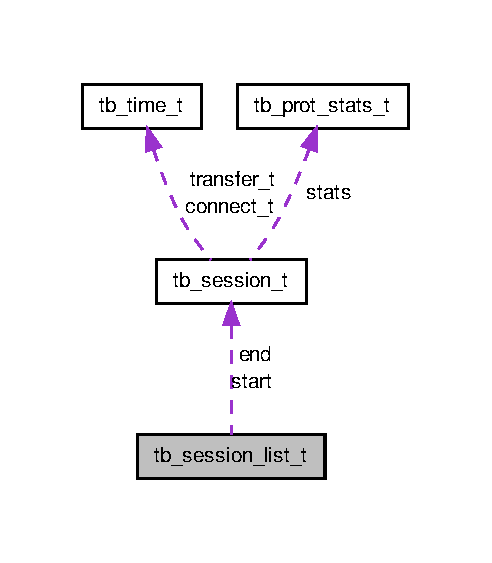
\includegraphics[width=236pt]{structtb__session__list__t__coll__graph}
\end{center}
\end{figure}
\subsection*{Data Fields}
\begin{DoxyCompactItemize}
\item 
int \hyperlink{structtb__session__list__t_a07d174b6514e5b02a3aa97ddc357d062}{current\-\_\-max\-\_\-id}
\item 
\hyperlink{structtb__session__t}{tb\-\_\-session\-\_\-t} $\ast$ \hyperlink{structtb__session__list__t_ae4ef1c5e563343eb946a3fe31c28be31}{start}
\item 
\hyperlink{structtb__session__t}{tb\-\_\-session\-\_\-t} $\ast$ \hyperlink{structtb__session__list__t_aab7b6dca3cae04438a12695d690d54c7}{end}
\end{DoxyCompactItemize}


\subsection{Detailed Description}


Definition at line 87 of file tb\-\_\-session.\-h.



\subsection{Field Documentation}
\hypertarget{structtb__session__list__t_a07d174b6514e5b02a3aa97ddc357d062}{\index{tb\-\_\-session\-\_\-list\-\_\-t@{tb\-\_\-session\-\_\-list\-\_\-t}!current\-\_\-max\-\_\-id@{current\-\_\-max\-\_\-id}}
\index{current\-\_\-max\-\_\-id@{current\-\_\-max\-\_\-id}!tb_session_list_t@{tb\-\_\-session\-\_\-list\-\_\-t}}
\subsubsection[{current\-\_\-max\-\_\-id}]{\setlength{\rightskip}{0pt plus 5cm}int current\-\_\-max\-\_\-id}}\label{structtb__session__list__t_a07d174b6514e5b02a3aa97ddc357d062}


Definition at line 89 of file tb\-\_\-session.\-h.

\hypertarget{structtb__session__list__t_aab7b6dca3cae04438a12695d690d54c7}{\index{tb\-\_\-session\-\_\-list\-\_\-t@{tb\-\_\-session\-\_\-list\-\_\-t}!end@{end}}
\index{end@{end}!tb_session_list_t@{tb\-\_\-session\-\_\-list\-\_\-t}}
\subsubsection[{end}]{\setlength{\rightskip}{0pt plus 5cm}{\bf tb\-\_\-session\-\_\-t}$\ast$ end}}\label{structtb__session__list__t_aab7b6dca3cae04438a12695d690d54c7}


Definition at line 91 of file tb\-\_\-session.\-h.

\hypertarget{structtb__session__list__t_ae4ef1c5e563343eb946a3fe31c28be31}{\index{tb\-\_\-session\-\_\-list\-\_\-t@{tb\-\_\-session\-\_\-list\-\_\-t}!start@{start}}
\index{start@{start}!tb_session_list_t@{tb\-\_\-session\-\_\-list\-\_\-t}}
\subsubsection[{start}]{\setlength{\rightskip}{0pt plus 5cm}{\bf tb\-\_\-session\-\_\-t}$\ast$ start}}\label{structtb__session__list__t_ae4ef1c5e563343eb946a3fe31c28be31}


Definition at line 90 of file tb\-\_\-session.\-h.



The documentation for this struct was generated from the following file\-:\begin{DoxyCompactItemize}
\item 
src/\hyperlink{tb__session_8h}{tb\-\_\-session.\-h}\end{DoxyCompactItemize}

\hypertarget{structtb__session__t}{\section{tb\-\_\-session\-\_\-t Struct Reference}
\label{structtb__session__t}\index{tb\-\_\-session\-\_\-t@{tb\-\_\-session\-\_\-t}}
}


{\ttfamily \#include $<$tb\-\_\-session.\-h$>$}



Collaboration diagram for tb\-\_\-session\-\_\-t\-:\nopagebreak
\begin{figure}[H]
\begin{center}
\leavevmode
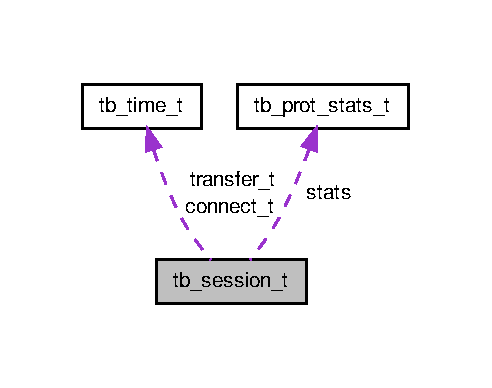
\includegraphics[width=236pt]{structtb__session__t__coll__graph}
\end{center}
\end{figure}
\subsection*{Data Fields}
\begin{DoxyCompactItemize}
\item 
int \hyperlink{structtb__session__t_a7441ef0865bcb3db9b8064dd7375c1ea}{id}
\begin{DoxyCompactList}\small\item\em Id for this session. \end{DoxyCompactList}\item 
char $\ast$ \hyperlink{structtb__session__t_a879a8cdf605d02f8af8b2e216b8764f2}{address}
\begin{DoxyCompactList}\small\item\em The address to connect/bind to. \end{DoxyCompactList}\item 
char $\ast$ \hyperlink{structtb__session__t_add99ba4ea70b8f66170823cad9a55fa4}{port}
\begin{DoxyCompactList}\small\item\em The port to connect/bind to. \end{DoxyCompactList}\item 
struct sockaddr\-\_\-storage $\ast$ \hyperlink{structtb__session__t_ab617a1bfa381136f3c0811b771c618e9}{addr\-\_\-in}
\begin{DoxyCompactList}\small\item\em For receiving connections. \end{DoxyCompactList}\item 
socklen\-\_\-t \hyperlink{structtb__session__t_a116941d922ae354d7241d04b0f3c84d8}{addr\-\_\-len}
\begin{DoxyCompactList}\small\item\em Length of sockaddr\-\_\-storage. \end{DoxyCompactList}\item 
struct addrinfo $\ast$ \hyperlink{structtb__session__t_aab742bc33815bd69bf49ad1861006b97}{addr\-\_\-info}
\begin{DoxyCompactList}\small\item\em Connection info. \end{DoxyCompactList}\item 
struct addrinfo $\ast$ \hyperlink{structtb__session__t_a105521cb94384edeaace1a1ce7b3d7c7}{addr\-\_\-hints}
\begin{DoxyCompactList}\small\item\em Connection hints. \end{DoxyCompactList}\item 
int \hyperlink{structtb__session__t_a94d540b145f21be2f9b28a2c225ccf30}{sock\-\_\-d}
\begin{DoxyCompactList}\small\item\em The socket descriptor for this session. \end{DoxyCompactList}\item 
int \hyperlink{structtb__session__t_af7112fe07fe05134febc994e10196ce5}{pack\-\_\-size}
\begin{DoxyCompactList}\small\item\em The size of the pack to use. \end{DoxyCompactList}\item 
char $\ast$ \hyperlink{structtb__session__t_a8505c513bc640d1f69e5f76fb32b24a8}{file\-\_\-name}
\item 
char $\ast$ \hyperlink{structtb__session__t_a91a70b77df95bd8b0830b49a094c2acb}{data}
\item 
size\-\_\-t \hyperlink{structtb__session__t_ad6bc120bffc64dfc5230863a8ba96596}{data\-\_\-size}
\item 
int \hyperlink{structtb__session__t_adf89a25c6c2cefbabf86ff4e7931032e}{int\-\_\-data}
\begin{DoxyCompactList}\small\item\em If the session creates the data, it is destroyed. \end{DoxyCompactList}\item 
int \hyperlink{structtb__session__t_ad3547e4d09ba01be9e898cf841504521}{last\-\_\-trans}
\item 
long long \hyperlink{structtb__session__t_af8b7f35061eb6fd4b3cda13b50755b89}{total\-\_\-bytes}
\item 
\hyperlink{structtb__prot__stats__t}{tb\-\_\-prot\-\_\-stats\-\_\-t} $\ast$ \hyperlink{structtb__session__t_a464593aa6d4c80e0f689c501c4e81e8c}{stats}
\item 
\hyperlink{tb__session_8h_a81168c33495c6f3db310119f82934596}{tb\-\_\-session\-\_\-status} \hyperlink{structtb__session__t_a92613ed83a3cc0d2644758af475d9782}{status}
\item 
int $\ast$ \hyperlink{structtb__session__t_a22cc288b7e9b2ffe6053aeac5914cb40}{l\-\_\-status}
\begin{DoxyCompactList}\small\item\em The status of the session. \end{DoxyCompactList}\item 
long long $\ast$ \hyperlink{structtb__session__t_a98701b8da6c02c1671dd748b2251cea7}{l\-\_\-txrx}
\item 
pthread\-\_\-t $\ast$ \hyperlink{structtb__session__t_ae0b73c023bde38042a32ba345baca741}{s\-\_\-thread}
\begin{DoxyCompactList}\small\item\em Thread for this session. \end{DoxyCompactList}\item 
pthread\-\_\-mutex\-\_\-t $\ast$ \hyperlink{structtb__session__t_ab828bf6b1b85621025b518a892b79d79}{stat\-\_\-lock}
\begin{DoxyCompactList}\small\item\em Lock for stat collection. \end{DoxyCompactList}\item 
void $\ast$ \hyperlink{structtb__session__t_ae96f976543c2fbc18fd89a368720f4d4}{n\-\_\-session}
\begin{DoxyCompactList}\small\item\em Link to next session (Linked list). \end{DoxyCompactList}\item 
\hyperlink{structtb__time__t}{tb\-\_\-time\-\_\-t} $\ast$ \hyperlink{structtb__session__t_a0cb6fc264a37771e927fe0b383fc600c}{transfer\-\_\-t}
\begin{DoxyCompactList}\small\item\em Transfer time. \end{DoxyCompactList}\item 
\hyperlink{structtb__time__t}{tb\-\_\-time\-\_\-t} $\ast$ \hyperlink{structtb__session__t_a49678949e63fd3a8335bac2bfa9d9ff2}{connect\-\_\-t}
\begin{DoxyCompactList}\small\item\em Connection time. \end{DoxyCompactList}\item 
void $\ast$ \hyperlink{structtb__session__t_acb1df3a0f703b05bc4971f79cabe2597}{info}
\end{DoxyCompactItemize}


\subsection{Detailed Description}


Definition at line 44 of file tb\-\_\-session.\-h.



\subsection{Field Documentation}
\hypertarget{structtb__session__t_a105521cb94384edeaace1a1ce7b3d7c7}{\index{tb\-\_\-session\-\_\-t@{tb\-\_\-session\-\_\-t}!addr\-\_\-hints@{addr\-\_\-hints}}
\index{addr\-\_\-hints@{addr\-\_\-hints}!tb_session_t@{tb\-\_\-session\-\_\-t}}
\subsubsection[{addr\-\_\-hints}]{\setlength{\rightskip}{0pt plus 5cm}struct addrinfo$\ast$ addr\-\_\-hints}}\label{structtb__session__t_a105521cb94384edeaace1a1ce7b3d7c7}


Connection hints. 



Definition at line 56 of file tb\-\_\-session.\-h.

\hypertarget{structtb__session__t_ab617a1bfa381136f3c0811b771c618e9}{\index{tb\-\_\-session\-\_\-t@{tb\-\_\-session\-\_\-t}!addr\-\_\-in@{addr\-\_\-in}}
\index{addr\-\_\-in@{addr\-\_\-in}!tb_session_t@{tb\-\_\-session\-\_\-t}}
\subsubsection[{addr\-\_\-in}]{\setlength{\rightskip}{0pt plus 5cm}struct sockaddr\-\_\-storage$\ast$ addr\-\_\-in}}\label{structtb__session__t_ab617a1bfa381136f3c0811b771c618e9}


For receiving connections. 



Definition at line 53 of file tb\-\_\-session.\-h.

\hypertarget{structtb__session__t_aab742bc33815bd69bf49ad1861006b97}{\index{tb\-\_\-session\-\_\-t@{tb\-\_\-session\-\_\-t}!addr\-\_\-info@{addr\-\_\-info}}
\index{addr\-\_\-info@{addr\-\_\-info}!tb_session_t@{tb\-\_\-session\-\_\-t}}
\subsubsection[{addr\-\_\-info}]{\setlength{\rightskip}{0pt plus 5cm}struct addrinfo$\ast$ addr\-\_\-info}}\label{structtb__session__t_aab742bc33815bd69bf49ad1861006b97}


Connection info. 



Definition at line 55 of file tb\-\_\-session.\-h.

\hypertarget{structtb__session__t_a116941d922ae354d7241d04b0f3c84d8}{\index{tb\-\_\-session\-\_\-t@{tb\-\_\-session\-\_\-t}!addr\-\_\-len@{addr\-\_\-len}}
\index{addr\-\_\-len@{addr\-\_\-len}!tb_session_t@{tb\-\_\-session\-\_\-t}}
\subsubsection[{addr\-\_\-len}]{\setlength{\rightskip}{0pt plus 5cm}socklen\-\_\-t addr\-\_\-len}}\label{structtb__session__t_a116941d922ae354d7241d04b0f3c84d8}


Length of sockaddr\-\_\-storage. 



Definition at line 54 of file tb\-\_\-session.\-h.

\hypertarget{structtb__session__t_a879a8cdf605d02f8af8b2e216b8764f2}{\index{tb\-\_\-session\-\_\-t@{tb\-\_\-session\-\_\-t}!address@{address}}
\index{address@{address}!tb_session_t@{tb\-\_\-session\-\_\-t}}
\subsubsection[{address}]{\setlength{\rightskip}{0pt plus 5cm}char$\ast$ address}}\label{structtb__session__t_a879a8cdf605d02f8af8b2e216b8764f2}


The address to connect/bind to. 



Definition at line 49 of file tb\-\_\-session.\-h.

\hypertarget{structtb__session__t_a49678949e63fd3a8335bac2bfa9d9ff2}{\index{tb\-\_\-session\-\_\-t@{tb\-\_\-session\-\_\-t}!connect\-\_\-t@{connect\-\_\-t}}
\index{connect\-\_\-t@{connect\-\_\-t}!tb_session_t@{tb\-\_\-session\-\_\-t}}
\subsubsection[{connect\-\_\-t}]{\setlength{\rightskip}{0pt plus 5cm}{\bf tb\-\_\-time\-\_\-t}$\ast$ connect\-\_\-t}}\label{structtb__session__t_a49678949e63fd3a8335bac2bfa9d9ff2}


Connection time. 



Definition at line 83 of file tb\-\_\-session.\-h.

\hypertarget{structtb__session__t_a91a70b77df95bd8b0830b49a094c2acb}{\index{tb\-\_\-session\-\_\-t@{tb\-\_\-session\-\_\-t}!data@{data}}
\index{data@{data}!tb_session_t@{tb\-\_\-session\-\_\-t}}
\subsubsection[{data}]{\setlength{\rightskip}{0pt plus 5cm}char$\ast$ data}}\label{structtb__session__t_a91a70b77df95bd8b0830b49a094c2acb}


Definition at line 62 of file tb\-\_\-session.\-h.

\hypertarget{structtb__session__t_ad6bc120bffc64dfc5230863a8ba96596}{\index{tb\-\_\-session\-\_\-t@{tb\-\_\-session\-\_\-t}!data\-\_\-size@{data\-\_\-size}}
\index{data\-\_\-size@{data\-\_\-size}!tb_session_t@{tb\-\_\-session\-\_\-t}}
\subsubsection[{data\-\_\-size}]{\setlength{\rightskip}{0pt plus 5cm}size\-\_\-t data\-\_\-size}}\label{structtb__session__t_ad6bc120bffc64dfc5230863a8ba96596}


Definition at line 63 of file tb\-\_\-session.\-h.

\hypertarget{structtb__session__t_a8505c513bc640d1f69e5f76fb32b24a8}{\index{tb\-\_\-session\-\_\-t@{tb\-\_\-session\-\_\-t}!file\-\_\-name@{file\-\_\-name}}
\index{file\-\_\-name@{file\-\_\-name}!tb_session_t@{tb\-\_\-session\-\_\-t}}
\subsubsection[{file\-\_\-name}]{\setlength{\rightskip}{0pt plus 5cm}char$\ast$ file\-\_\-name}}\label{structtb__session__t_a8505c513bc640d1f69e5f76fb32b24a8}


Definition at line 61 of file tb\-\_\-session.\-h.

\hypertarget{structtb__session__t_a7441ef0865bcb3db9b8064dd7375c1ea}{\index{tb\-\_\-session\-\_\-t@{tb\-\_\-session\-\_\-t}!id@{id}}
\index{id@{id}!tb_session_t@{tb\-\_\-session\-\_\-t}}
\subsubsection[{id}]{\setlength{\rightskip}{0pt plus 5cm}int id}}\label{structtb__session__t_a7441ef0865bcb3db9b8064dd7375c1ea}


Id for this session. 



Definition at line 46 of file tb\-\_\-session.\-h.

\hypertarget{structtb__session__t_acb1df3a0f703b05bc4971f79cabe2597}{\index{tb\-\_\-session\-\_\-t@{tb\-\_\-session\-\_\-t}!info@{info}}
\index{info@{info}!tb_session_t@{tb\-\_\-session\-\_\-t}}
\subsubsection[{info}]{\setlength{\rightskip}{0pt plus 5cm}void$\ast$ info}}\label{structtb__session__t_acb1df3a0f703b05bc4971f79cabe2597}


Definition at line 86 of file tb\-\_\-session.\-h.

\hypertarget{structtb__session__t_adf89a25c6c2cefbabf86ff4e7931032e}{\index{tb\-\_\-session\-\_\-t@{tb\-\_\-session\-\_\-t}!int\-\_\-data@{int\-\_\-data}}
\index{int\-\_\-data@{int\-\_\-data}!tb_session_t@{tb\-\_\-session\-\_\-t}}
\subsubsection[{int\-\_\-data}]{\setlength{\rightskip}{0pt plus 5cm}int int\-\_\-data}}\label{structtb__session__t_adf89a25c6c2cefbabf86ff4e7931032e}


If the session creates the data, it is destroyed. 



Definition at line 64 of file tb\-\_\-session.\-h.

\hypertarget{structtb__session__t_a22cc288b7e9b2ffe6053aeac5914cb40}{\index{tb\-\_\-session\-\_\-t@{tb\-\_\-session\-\_\-t}!l\-\_\-status@{l\-\_\-status}}
\index{l\-\_\-status@{l\-\_\-status}!tb_session_t@{tb\-\_\-session\-\_\-t}}
\subsubsection[{l\-\_\-status}]{\setlength{\rightskip}{0pt plus 5cm}int$\ast$ l\-\_\-status}}\label{structtb__session__t_a22cc288b7e9b2ffe6053aeac5914cb40}


The status of the session. 



Definition at line 73 of file tb\-\_\-session.\-h.

\hypertarget{structtb__session__t_a98701b8da6c02c1671dd748b2251cea7}{\index{tb\-\_\-session\-\_\-t@{tb\-\_\-session\-\_\-t}!l\-\_\-txrx@{l\-\_\-txrx}}
\index{l\-\_\-txrx@{l\-\_\-txrx}!tb_session_t@{tb\-\_\-session\-\_\-t}}
\subsubsection[{l\-\_\-txrx}]{\setlength{\rightskip}{0pt plus 5cm}long long$\ast$ l\-\_\-txrx}}\label{structtb__session__t_a98701b8da6c02c1671dd748b2251cea7}


Definition at line 74 of file tb\-\_\-session.\-h.

\hypertarget{structtb__session__t_ad3547e4d09ba01be9e898cf841504521}{\index{tb\-\_\-session\-\_\-t@{tb\-\_\-session\-\_\-t}!last\-\_\-trans@{last\-\_\-trans}}
\index{last\-\_\-trans@{last\-\_\-trans}!tb_session_t@{tb\-\_\-session\-\_\-t}}
\subsubsection[{last\-\_\-trans}]{\setlength{\rightskip}{0pt plus 5cm}int last\-\_\-trans}}\label{structtb__session__t_ad3547e4d09ba01be9e898cf841504521}


Definition at line 67 of file tb\-\_\-session.\-h.

\hypertarget{structtb__session__t_ae96f976543c2fbc18fd89a368720f4d4}{\index{tb\-\_\-session\-\_\-t@{tb\-\_\-session\-\_\-t}!n\-\_\-session@{n\-\_\-session}}
\index{n\-\_\-session@{n\-\_\-session}!tb_session_t@{tb\-\_\-session\-\_\-t}}
\subsubsection[{n\-\_\-session}]{\setlength{\rightskip}{0pt plus 5cm}void$\ast$ n\-\_\-session}}\label{structtb__session__t_ae96f976543c2fbc18fd89a368720f4d4}


Link to next session (Linked list). 



Definition at line 79 of file tb\-\_\-session.\-h.

\hypertarget{structtb__session__t_af7112fe07fe05134febc994e10196ce5}{\index{tb\-\_\-session\-\_\-t@{tb\-\_\-session\-\_\-t}!pack\-\_\-size@{pack\-\_\-size}}
\index{pack\-\_\-size@{pack\-\_\-size}!tb_session_t@{tb\-\_\-session\-\_\-t}}
\subsubsection[{pack\-\_\-size}]{\setlength{\rightskip}{0pt plus 5cm}int pack\-\_\-size}}\label{structtb__session__t_af7112fe07fe05134febc994e10196ce5}


The size of the pack to use. 



Definition at line 58 of file tb\-\_\-session.\-h.

\hypertarget{structtb__session__t_add99ba4ea70b8f66170823cad9a55fa4}{\index{tb\-\_\-session\-\_\-t@{tb\-\_\-session\-\_\-t}!port@{port}}
\index{port@{port}!tb_session_t@{tb\-\_\-session\-\_\-t}}
\subsubsection[{port}]{\setlength{\rightskip}{0pt plus 5cm}char$\ast$ port}}\label{structtb__session__t_add99ba4ea70b8f66170823cad9a55fa4}


The port to connect/bind to. 



Definition at line 50 of file tb\-\_\-session.\-h.

\hypertarget{structtb__session__t_ae0b73c023bde38042a32ba345baca741}{\index{tb\-\_\-session\-\_\-t@{tb\-\_\-session\-\_\-t}!s\-\_\-thread@{s\-\_\-thread}}
\index{s\-\_\-thread@{s\-\_\-thread}!tb_session_t@{tb\-\_\-session\-\_\-t}}
\subsubsection[{s\-\_\-thread}]{\setlength{\rightskip}{0pt plus 5cm}pthread\-\_\-t$\ast$ s\-\_\-thread}}\label{structtb__session__t_ae0b73c023bde38042a32ba345baca741}


Thread for this session. 



Definition at line 77 of file tb\-\_\-session.\-h.

\hypertarget{structtb__session__t_a94d540b145f21be2f9b28a2c225ccf30}{\index{tb\-\_\-session\-\_\-t@{tb\-\_\-session\-\_\-t}!sock\-\_\-d@{sock\-\_\-d}}
\index{sock\-\_\-d@{sock\-\_\-d}!tb_session_t@{tb\-\_\-session\-\_\-t}}
\subsubsection[{sock\-\_\-d}]{\setlength{\rightskip}{0pt plus 5cm}int sock\-\_\-d}}\label{structtb__session__t_a94d540b145f21be2f9b28a2c225ccf30}


The socket descriptor for this session. 



Definition at line 57 of file tb\-\_\-session.\-h.

\hypertarget{structtb__session__t_ab828bf6b1b85621025b518a892b79d79}{\index{tb\-\_\-session\-\_\-t@{tb\-\_\-session\-\_\-t}!stat\-\_\-lock@{stat\-\_\-lock}}
\index{stat\-\_\-lock@{stat\-\_\-lock}!tb_session_t@{tb\-\_\-session\-\_\-t}}
\subsubsection[{stat\-\_\-lock}]{\setlength{\rightskip}{0pt plus 5cm}pthread\-\_\-mutex\-\_\-t$\ast$ stat\-\_\-lock}}\label{structtb__session__t_ab828bf6b1b85621025b518a892b79d79}


Lock for stat collection. 



Definition at line 78 of file tb\-\_\-session.\-h.

\hypertarget{structtb__session__t_a464593aa6d4c80e0f689c501c4e81e8c}{\index{tb\-\_\-session\-\_\-t@{tb\-\_\-session\-\_\-t}!stats@{stats}}
\index{stats@{stats}!tb_session_t@{tb\-\_\-session\-\_\-t}}
\subsubsection[{stats}]{\setlength{\rightskip}{0pt plus 5cm}{\bf tb\-\_\-prot\-\_\-stats\-\_\-t}$\ast$ stats}}\label{structtb__session__t_a464593aa6d4c80e0f689c501c4e81e8c}


Definition at line 69 of file tb\-\_\-session.\-h.

\hypertarget{structtb__session__t_a92613ed83a3cc0d2644758af475d9782}{\index{tb\-\_\-session\-\_\-t@{tb\-\_\-session\-\_\-t}!status@{status}}
\index{status@{status}!tb_session_t@{tb\-\_\-session\-\_\-t}}
\subsubsection[{status}]{\setlength{\rightskip}{0pt plus 5cm}{\bf tb\-\_\-session\-\_\-status} status}}\label{structtb__session__t_a92613ed83a3cc0d2644758af475d9782}


Definition at line 72 of file tb\-\_\-session.\-h.

\hypertarget{structtb__session__t_af8b7f35061eb6fd4b3cda13b50755b89}{\index{tb\-\_\-session\-\_\-t@{tb\-\_\-session\-\_\-t}!total\-\_\-bytes@{total\-\_\-bytes}}
\index{total\-\_\-bytes@{total\-\_\-bytes}!tb_session_t@{tb\-\_\-session\-\_\-t}}
\subsubsection[{total\-\_\-bytes}]{\setlength{\rightskip}{0pt plus 5cm}long long total\-\_\-bytes}}\label{structtb__session__t_af8b7f35061eb6fd4b3cda13b50755b89}


Definition at line 68 of file tb\-\_\-session.\-h.

\hypertarget{structtb__session__t_a0cb6fc264a37771e927fe0b383fc600c}{\index{tb\-\_\-session\-\_\-t@{tb\-\_\-session\-\_\-t}!transfer\-\_\-t@{transfer\-\_\-t}}
\index{transfer\-\_\-t@{transfer\-\_\-t}!tb_session_t@{tb\-\_\-session\-\_\-t}}
\subsubsection[{transfer\-\_\-t}]{\setlength{\rightskip}{0pt plus 5cm}{\bf tb\-\_\-time\-\_\-t}$\ast$ transfer\-\_\-t}}\label{structtb__session__t_a0cb6fc264a37771e927fe0b383fc600c}


Transfer time. 



Definition at line 82 of file tb\-\_\-session.\-h.



The documentation for this struct was generated from the following file\-:\begin{DoxyCompactItemize}
\item 
src/\hyperlink{tb__session_8h}{tb\-\_\-session.\-h}\end{DoxyCompactItemize}

\hypertarget{structtb__test__params__t}{\section{tb\-\_\-test\-\_\-params\-\_\-t Struct Reference}
\label{structtb__test__params__t}\index{tb\-\_\-test\-\_\-params\-\_\-t@{tb\-\_\-test\-\_\-params\-\_\-t}}
}


{\ttfamily \#include $<$tb\-\_\-listener.\-h$>$}

\subsection*{Data Fields}
\begin{DoxyCompactItemize}
\item 
\hyperlink{tb__listener_8h_ae37f3ebcf0081b2dd11adf41f1f867d6}{E\-N\-D\-P\-O\-I\-N\-T\-\_\-\-T\-Y\-P\-E} \hyperlink{structtb__test__params__t_a3fefae1824d77098e05df5bac09c1791}{type}
\begin{DoxyCompactList}\small\item\em The end point type. \end{DoxyCompactList}\item 
\hyperlink{tb__protocol_8h_a7a5bff1040fc154c510874327d44cc1a}{P\-R\-O\-T\-O\-C\-O\-L} \hyperlink{structtb__test__params__t_a0d2276cd987e688180eedab183cd503e}{protocol}
\begin{DoxyCompactList}\small\item\em The protocol to test. \end{DoxyCompactList}\item 
\hyperlink{tb__protocol_8h_ac5355051296d54a114b8691ccfc4010c}{C\-O\-N\-G\-E\-S\-T\-I\-O\-N\-\_\-\-C\-O\-N\-T\-R\-O\-L} \hyperlink{structtb__test__params__t_a50b4d1da7c10bfd1e9365a1c37d09442}{control}
\begin{DoxyCompactList}\small\item\em The congestion control algorithm to use. \end{DoxyCompactList}\item 
char $\ast$ \hyperlink{structtb__test__params__t_a879a8cdf605d02f8af8b2e216b8764f2}{address}
\begin{DoxyCompactList}\small\item\em The address to bind/connect to. \end{DoxyCompactList}\item 
char $\ast$ \hyperlink{structtb__test__params__t_add99ba4ea70b8f66170823cad9a55fa4}{port}
\begin{DoxyCompactList}\small\item\em The port to bind/connect to. \end{DoxyCompactList}\item 
int \hyperlink{structtb__test__params__t_a8ae9ae9a85fbb77bc460b0d43e4fc1c5}{l4\-\_\-r\-\_\-b\-\_\-size}
\begin{DoxyCompactList}\small\item\em The size of the l4 read buffer. \end{DoxyCompactList}\item 
int \hyperlink{structtb__test__params__t_a97320ff488c6ed44b28b034c826482c7}{l4\-\_\-w\-\_\-b\-\_\-size}
\begin{DoxyCompactList}\small\item\em The size of the l4 write buffer. \end{DoxyCompactList}\item 
int \hyperlink{structtb__test__params__t_aa9d1ab0c9c6ef33a4b6bd60172dd0ec5}{l3\-\_\-r\-\_\-b\-\_\-size}
\begin{DoxyCompactList}\small\item\em The size of the l3 read buffer. \end{DoxyCompactList}\item 
int \hyperlink{structtb__test__params__t_aee0e87ac541b0694deb1499aa3371f91}{l3\-\_\-w\-\_\-b\-\_\-size}
\begin{DoxyCompactList}\small\item\em The size of the l3 write buffer. \end{DoxyCompactList}\item 
int \hyperlink{structtb__test__params__t_a848d9c2765e62bac90bee8355062858a}{d\-\_\-size}
\begin{DoxyCompactList}\small\item\em The size of the data to send. \end{DoxyCompactList}\item 
char $\ast$ \hyperlink{structtb__test__params__t_a8505c513bc640d1f69e5f76fb32b24a8}{file\-\_\-name}
\begin{DoxyCompactList}\small\item\em The name of the file to use. \end{DoxyCompactList}\item 
int \hyperlink{structtb__test__params__t_a093a636a4cc3aec4f564b9ab29081b59}{d\-\_\-on\-\_\-exit}
\begin{DoxyCompactList}\small\item\em Destroy the listener on exit. \end{DoxyCompactList}\item 
int \hyperlink{structtb__test__params__t_a46fa1969de5714507943035793d36269}{monitor}
\begin{DoxyCompactList}\small\item\em Monitor the connection. \end{DoxyCompactList}\item 
int \hyperlink{structtb__test__params__t_a21a0be842e8fa2c780fa87f45bd5d17e}{print\-\_\-stats}
\begin{DoxyCompactList}\small\item\em Print stats to screen. \end{DoxyCompactList}\item 
int \hyperlink{structtb__test__params__t_ac5bfaec8717601161bb642175e1d85e0}{log\-\_\-enable}
\begin{DoxyCompactList}\small\item\em Enable logging. \end{DoxyCompactList}\item 
char $\ast$ \hyperlink{structtb__test__params__t_ac0ddb52991004ce37e7ef093186f44a1}{log\-\_\-path}
\begin{DoxyCompactList}\small\item\em The path to save the log to. \end{DoxyCompactList}\item 
int \hyperlink{structtb__test__params__t_af7112fe07fe05134febc994e10196ce5}{pack\-\_\-size}
\end{DoxyCompactItemize}


\subsection{Detailed Description}


Definition at line 78 of file tb\-\_\-listener.\-h.



\subsection{Field Documentation}
\hypertarget{structtb__test__params__t_a879a8cdf605d02f8af8b2e216b8764f2}{\index{tb\-\_\-test\-\_\-params\-\_\-t@{tb\-\_\-test\-\_\-params\-\_\-t}!address@{address}}
\index{address@{address}!tb_test_params_t@{tb\-\_\-test\-\_\-params\-\_\-t}}
\subsubsection[{address}]{\setlength{\rightskip}{0pt plus 5cm}char$\ast$ address}}\label{structtb__test__params__t_a879a8cdf605d02f8af8b2e216b8764f2}


The address to bind/connect to. 



Definition at line 85 of file tb\-\_\-listener.\-h.

\hypertarget{structtb__test__params__t_a50b4d1da7c10bfd1e9365a1c37d09442}{\index{tb\-\_\-test\-\_\-params\-\_\-t@{tb\-\_\-test\-\_\-params\-\_\-t}!control@{control}}
\index{control@{control}!tb_test_params_t@{tb\-\_\-test\-\_\-params\-\_\-t}}
\subsubsection[{control}]{\setlength{\rightskip}{0pt plus 5cm}{\bf C\-O\-N\-G\-E\-S\-T\-I\-O\-N\-\_\-\-C\-O\-N\-T\-R\-O\-L} control}}\label{structtb__test__params__t_a50b4d1da7c10bfd1e9365a1c37d09442}


The congestion control algorithm to use. 



Definition at line 82 of file tb\-\_\-listener.\-h.

\hypertarget{structtb__test__params__t_a093a636a4cc3aec4f564b9ab29081b59}{\index{tb\-\_\-test\-\_\-params\-\_\-t@{tb\-\_\-test\-\_\-params\-\_\-t}!d\-\_\-on\-\_\-exit@{d\-\_\-on\-\_\-exit}}
\index{d\-\_\-on\-\_\-exit@{d\-\_\-on\-\_\-exit}!tb_test_params_t@{tb\-\_\-test\-\_\-params\-\_\-t}}
\subsubsection[{d\-\_\-on\-\_\-exit}]{\setlength{\rightskip}{0pt plus 5cm}int d\-\_\-on\-\_\-exit}}\label{structtb__test__params__t_a093a636a4cc3aec4f564b9ab29081b59}


Destroy the listener on exit. 



Definition at line 100 of file tb\-\_\-listener.\-h.

\hypertarget{structtb__test__params__t_a848d9c2765e62bac90bee8355062858a}{\index{tb\-\_\-test\-\_\-params\-\_\-t@{tb\-\_\-test\-\_\-params\-\_\-t}!d\-\_\-size@{d\-\_\-size}}
\index{d\-\_\-size@{d\-\_\-size}!tb_test_params_t@{tb\-\_\-test\-\_\-params\-\_\-t}}
\subsubsection[{d\-\_\-size}]{\setlength{\rightskip}{0pt plus 5cm}int d\-\_\-size}}\label{structtb__test__params__t_a848d9c2765e62bac90bee8355062858a}


The size of the data to send. 



Definition at line 96 of file tb\-\_\-listener.\-h.

\hypertarget{structtb__test__params__t_a8505c513bc640d1f69e5f76fb32b24a8}{\index{tb\-\_\-test\-\_\-params\-\_\-t@{tb\-\_\-test\-\_\-params\-\_\-t}!file\-\_\-name@{file\-\_\-name}}
\index{file\-\_\-name@{file\-\_\-name}!tb_test_params_t@{tb\-\_\-test\-\_\-params\-\_\-t}}
\subsubsection[{file\-\_\-name}]{\setlength{\rightskip}{0pt plus 5cm}char$\ast$ file\-\_\-name}}\label{structtb__test__params__t_a8505c513bc640d1f69e5f76fb32b24a8}


The name of the file to use. 



Definition at line 97 of file tb\-\_\-listener.\-h.

\hypertarget{structtb__test__params__t_aa9d1ab0c9c6ef33a4b6bd60172dd0ec5}{\index{tb\-\_\-test\-\_\-params\-\_\-t@{tb\-\_\-test\-\_\-params\-\_\-t}!l3\-\_\-r\-\_\-b\-\_\-size@{l3\-\_\-r\-\_\-b\-\_\-size}}
\index{l3\-\_\-r\-\_\-b\-\_\-size@{l3\-\_\-r\-\_\-b\-\_\-size}!tb_test_params_t@{tb\-\_\-test\-\_\-params\-\_\-t}}
\subsubsection[{l3\-\_\-r\-\_\-b\-\_\-size}]{\setlength{\rightskip}{0pt plus 5cm}int l3\-\_\-r\-\_\-b\-\_\-size}}\label{structtb__test__params__t_aa9d1ab0c9c6ef33a4b6bd60172dd0ec5}


The size of the l3 read buffer. 



Definition at line 92 of file tb\-\_\-listener.\-h.

\hypertarget{structtb__test__params__t_aee0e87ac541b0694deb1499aa3371f91}{\index{tb\-\_\-test\-\_\-params\-\_\-t@{tb\-\_\-test\-\_\-params\-\_\-t}!l3\-\_\-w\-\_\-b\-\_\-size@{l3\-\_\-w\-\_\-b\-\_\-size}}
\index{l3\-\_\-w\-\_\-b\-\_\-size@{l3\-\_\-w\-\_\-b\-\_\-size}!tb_test_params_t@{tb\-\_\-test\-\_\-params\-\_\-t}}
\subsubsection[{l3\-\_\-w\-\_\-b\-\_\-size}]{\setlength{\rightskip}{0pt plus 5cm}int l3\-\_\-w\-\_\-b\-\_\-size}}\label{structtb__test__params__t_aee0e87ac541b0694deb1499aa3371f91}


The size of the l3 write buffer. 



Definition at line 93 of file tb\-\_\-listener.\-h.

\hypertarget{structtb__test__params__t_a8ae9ae9a85fbb77bc460b0d43e4fc1c5}{\index{tb\-\_\-test\-\_\-params\-\_\-t@{tb\-\_\-test\-\_\-params\-\_\-t}!l4\-\_\-r\-\_\-b\-\_\-size@{l4\-\_\-r\-\_\-b\-\_\-size}}
\index{l4\-\_\-r\-\_\-b\-\_\-size@{l4\-\_\-r\-\_\-b\-\_\-size}!tb_test_params_t@{tb\-\_\-test\-\_\-params\-\_\-t}}
\subsubsection[{l4\-\_\-r\-\_\-b\-\_\-size}]{\setlength{\rightskip}{0pt plus 5cm}int l4\-\_\-r\-\_\-b\-\_\-size}}\label{structtb__test__params__t_a8ae9ae9a85fbb77bc460b0d43e4fc1c5}


The size of the l4 read buffer. 



Definition at line 89 of file tb\-\_\-listener.\-h.

\hypertarget{structtb__test__params__t_a97320ff488c6ed44b28b034c826482c7}{\index{tb\-\_\-test\-\_\-params\-\_\-t@{tb\-\_\-test\-\_\-params\-\_\-t}!l4\-\_\-w\-\_\-b\-\_\-size@{l4\-\_\-w\-\_\-b\-\_\-size}}
\index{l4\-\_\-w\-\_\-b\-\_\-size@{l4\-\_\-w\-\_\-b\-\_\-size}!tb_test_params_t@{tb\-\_\-test\-\_\-params\-\_\-t}}
\subsubsection[{l4\-\_\-w\-\_\-b\-\_\-size}]{\setlength{\rightskip}{0pt plus 5cm}int l4\-\_\-w\-\_\-b\-\_\-size}}\label{structtb__test__params__t_a97320ff488c6ed44b28b034c826482c7}


The size of the l4 write buffer. 



Definition at line 90 of file tb\-\_\-listener.\-h.

\hypertarget{structtb__test__params__t_ac5bfaec8717601161bb642175e1d85e0}{\index{tb\-\_\-test\-\_\-params\-\_\-t@{tb\-\_\-test\-\_\-params\-\_\-t}!log\-\_\-enable@{log\-\_\-enable}}
\index{log\-\_\-enable@{log\-\_\-enable}!tb_test_params_t@{tb\-\_\-test\-\_\-params\-\_\-t}}
\subsubsection[{log\-\_\-enable}]{\setlength{\rightskip}{0pt plus 5cm}int log\-\_\-enable}}\label{structtb__test__params__t_ac5bfaec8717601161bb642175e1d85e0}


Enable logging. 



Definition at line 107 of file tb\-\_\-listener.\-h.

\hypertarget{structtb__test__params__t_ac0ddb52991004ce37e7ef093186f44a1}{\index{tb\-\_\-test\-\_\-params\-\_\-t@{tb\-\_\-test\-\_\-params\-\_\-t}!log\-\_\-path@{log\-\_\-path}}
\index{log\-\_\-path@{log\-\_\-path}!tb_test_params_t@{tb\-\_\-test\-\_\-params\-\_\-t}}
\subsubsection[{log\-\_\-path}]{\setlength{\rightskip}{0pt plus 5cm}char$\ast$ log\-\_\-path}}\label{structtb__test__params__t_ac0ddb52991004ce37e7ef093186f44a1}


The path to save the log to. 



Definition at line 108 of file tb\-\_\-listener.\-h.

\hypertarget{structtb__test__params__t_a46fa1969de5714507943035793d36269}{\index{tb\-\_\-test\-\_\-params\-\_\-t@{tb\-\_\-test\-\_\-params\-\_\-t}!monitor@{monitor}}
\index{monitor@{monitor}!tb_test_params_t@{tb\-\_\-test\-\_\-params\-\_\-t}}
\subsubsection[{monitor}]{\setlength{\rightskip}{0pt plus 5cm}int monitor}}\label{structtb__test__params__t_a46fa1969de5714507943035793d36269}


Monitor the connection. 



Definition at line 103 of file tb\-\_\-listener.\-h.

\hypertarget{structtb__test__params__t_af7112fe07fe05134febc994e10196ce5}{\index{tb\-\_\-test\-\_\-params\-\_\-t@{tb\-\_\-test\-\_\-params\-\_\-t}!pack\-\_\-size@{pack\-\_\-size}}
\index{pack\-\_\-size@{pack\-\_\-size}!tb_test_params_t@{tb\-\_\-test\-\_\-params\-\_\-t}}
\subsubsection[{pack\-\_\-size}]{\setlength{\rightskip}{0pt plus 5cm}int pack\-\_\-size}}\label{structtb__test__params__t_af7112fe07fe05134febc994e10196ce5}


Definition at line 111 of file tb\-\_\-listener.\-h.

\hypertarget{structtb__test__params__t_add99ba4ea70b8f66170823cad9a55fa4}{\index{tb\-\_\-test\-\_\-params\-\_\-t@{tb\-\_\-test\-\_\-params\-\_\-t}!port@{port}}
\index{port@{port}!tb_test_params_t@{tb\-\_\-test\-\_\-params\-\_\-t}}
\subsubsection[{port}]{\setlength{\rightskip}{0pt plus 5cm}char$\ast$ port}}\label{structtb__test__params__t_add99ba4ea70b8f66170823cad9a55fa4}


The port to bind/connect to. 



Definition at line 86 of file tb\-\_\-listener.\-h.

\hypertarget{structtb__test__params__t_a21a0be842e8fa2c780fa87f45bd5d17e}{\index{tb\-\_\-test\-\_\-params\-\_\-t@{tb\-\_\-test\-\_\-params\-\_\-t}!print\-\_\-stats@{print\-\_\-stats}}
\index{print\-\_\-stats@{print\-\_\-stats}!tb_test_params_t@{tb\-\_\-test\-\_\-params\-\_\-t}}
\subsubsection[{print\-\_\-stats}]{\setlength{\rightskip}{0pt plus 5cm}int print\-\_\-stats}}\label{structtb__test__params__t_a21a0be842e8fa2c780fa87f45bd5d17e}


Print stats to screen. 



Definition at line 104 of file tb\-\_\-listener.\-h.

\hypertarget{structtb__test__params__t_a0d2276cd987e688180eedab183cd503e}{\index{tb\-\_\-test\-\_\-params\-\_\-t@{tb\-\_\-test\-\_\-params\-\_\-t}!protocol@{protocol}}
\index{protocol@{protocol}!tb_test_params_t@{tb\-\_\-test\-\_\-params\-\_\-t}}
\subsubsection[{protocol}]{\setlength{\rightskip}{0pt plus 5cm}{\bf P\-R\-O\-T\-O\-C\-O\-L} protocol}}\label{structtb__test__params__t_a0d2276cd987e688180eedab183cd503e}


The protocol to test. 



Definition at line 81 of file tb\-\_\-listener.\-h.

\hypertarget{structtb__test__params__t_a3fefae1824d77098e05df5bac09c1791}{\index{tb\-\_\-test\-\_\-params\-\_\-t@{tb\-\_\-test\-\_\-params\-\_\-t}!type@{type}}
\index{type@{type}!tb_test_params_t@{tb\-\_\-test\-\_\-params\-\_\-t}}
\subsubsection[{type}]{\setlength{\rightskip}{0pt plus 5cm}{\bf E\-N\-D\-P\-O\-I\-N\-T\-\_\-\-T\-Y\-P\-E} type}}\label{structtb__test__params__t_a3fefae1824d77098e05df5bac09c1791}


The end point type. 



Definition at line 80 of file tb\-\_\-listener.\-h.



The documentation for this struct was generated from the following file\-:\begin{DoxyCompactItemize}
\item 
src/\hyperlink{tb__listener_8h}{tb\-\_\-listener.\-h}\end{DoxyCompactItemize}

\hypertarget{structtb__time__t}{\section{tb\-\_\-time\-\_\-t Struct Reference}
\label{structtb__time__t}\index{tb\-\_\-time\-\_\-t@{tb\-\_\-time\-\_\-t}}
}


A struct to hold start, stop and elapsed times.  




{\ttfamily \#include $<$tb\-\_\-common.\-h$>$}

\subsection*{Data Fields}
\begin{DoxyCompactItemize}
\item 
clockid\-\_\-t \hyperlink{structtb__time__t_aa8e00f6c852df6521630cfa00531c02d}{clk\-\_\-id}
\item 
struct timespec $\ast$ \hyperlink{structtb__time__t_a300f258f56b552b672396bfbede700a8}{start}
\item 
struct timespec $\ast$ \hyperlink{structtb__time__t_a48fdbc276d8f5d2f81ebe02d2ff62473}{finish}
\item 
long long \hyperlink{structtb__time__t_a8889de00f0d94d229d5549cd57597948}{n\-\_\-sec}
\end{DoxyCompactItemize}


\subsection{Detailed Description}
A struct to hold start, stop and elapsed times. 

Definition at line 51 of file tb\-\_\-common.\-h.



\subsection{Field Documentation}
\hypertarget{structtb__time__t_aa8e00f6c852df6521630cfa00531c02d}{\index{tb\-\_\-time\-\_\-t@{tb\-\_\-time\-\_\-t}!clk\-\_\-id@{clk\-\_\-id}}
\index{clk\-\_\-id@{clk\-\_\-id}!tb_time_t@{tb\-\_\-time\-\_\-t}}
\subsubsection[{clk\-\_\-id}]{\setlength{\rightskip}{0pt plus 5cm}clockid\-\_\-t clk\-\_\-id}}\label{structtb__time__t_aa8e00f6c852df6521630cfa00531c02d}


Definition at line 53 of file tb\-\_\-common.\-h.

\hypertarget{structtb__time__t_a48fdbc276d8f5d2f81ebe02d2ff62473}{\index{tb\-\_\-time\-\_\-t@{tb\-\_\-time\-\_\-t}!finish@{finish}}
\index{finish@{finish}!tb_time_t@{tb\-\_\-time\-\_\-t}}
\subsubsection[{finish}]{\setlength{\rightskip}{0pt plus 5cm}struct timespec$\ast$ finish}}\label{structtb__time__t_a48fdbc276d8f5d2f81ebe02d2ff62473}


Definition at line 55 of file tb\-\_\-common.\-h.

\hypertarget{structtb__time__t_a8889de00f0d94d229d5549cd57597948}{\index{tb\-\_\-time\-\_\-t@{tb\-\_\-time\-\_\-t}!n\-\_\-sec@{n\-\_\-sec}}
\index{n\-\_\-sec@{n\-\_\-sec}!tb_time_t@{tb\-\_\-time\-\_\-t}}
\subsubsection[{n\-\_\-sec}]{\setlength{\rightskip}{0pt plus 5cm}long long n\-\_\-sec}}\label{structtb__time__t_a8889de00f0d94d229d5549cd57597948}


Definition at line 57 of file tb\-\_\-common.\-h.

\hypertarget{structtb__time__t_a300f258f56b552b672396bfbede700a8}{\index{tb\-\_\-time\-\_\-t@{tb\-\_\-time\-\_\-t}!start@{start}}
\index{start@{start}!tb_time_t@{tb\-\_\-time\-\_\-t}}
\subsubsection[{start}]{\setlength{\rightskip}{0pt plus 5cm}struct timespec$\ast$ start}}\label{structtb__time__t_a300f258f56b552b672396bfbede700a8}


Definition at line 54 of file tb\-\_\-common.\-h.



The documentation for this struct was generated from the following file\-:\begin{DoxyCompactItemize}
\item 
src/\hyperlink{tb__common_8h}{tb\-\_\-common.\-h}\end{DoxyCompactItemize}

\hypertarget{structtb__utp__t}{\section{tb\-\_\-utp\-\_\-t Struct Reference}
\label{structtb__utp__t}\index{tb\-\_\-utp\-\_\-t@{tb\-\_\-utp\-\_\-t}}
}


{\ttfamily \#include $<$tb\-\_\-utp.\-h$>$}



Collaboration diagram for tb\-\_\-utp\-\_\-t\-:\nopagebreak
\begin{figure}[H]
\begin{center}
\leavevmode
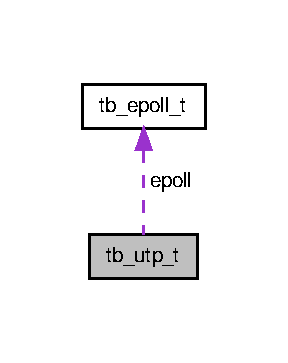
\includegraphics[width=138pt]{structtb__utp__t__coll__graph}
\end{center}
\end{figure}
\subsection*{Data Fields}
\begin{DoxyCompactItemize}
\item 
int \hyperlink{structtb__utp__t_a7441ef0865bcb3db9b8064dd7375c1ea}{id}
\begin{DoxyCompactList}\small\item\em Id for this utp struct. \end{DoxyCompactList}\item 
struct U\-T\-P\-Socket $\ast$ \hyperlink{structtb__utp__t_add15e39a83c7a0c72140c305bdd386d0}{socket}
\item 
int \hyperlink{structtb__utp__t_a514331e6141a28289f8ddead55eadebd}{sock\-\_\-fd}
\item 
char $\ast$ \hyperlink{structtb__utp__t_aff2566f4c366b48d73479bef43ee4d2e}{buffer}
\item 
char $\ast$ \hyperlink{structtb__utp__t_a2e6fac18f9532108c2aa44a52d3c6d67}{rec\-\_\-buffer}
\item 
int \hyperlink{structtb__utp__t_aeb56438a9cac1febce2dcddd6c404759}{read\-\_\-bytes}
\item 
int \hyperlink{structtb__utp__t_a814ec097a6a396e10f9f0924e924684e}{write\-\_\-bytes}
\item 
int \hyperlink{structtb__utp__t_af22ff4ab7a026e6c3b4b08eafb2df027}{buffer\-\_\-size}
\item 
int \hyperlink{structtb__utp__t_a57c1edf513c216e498e37e3428180480}{rec\-\_\-buff\-\_\-size}
\item 
int \hyperlink{structtb__utp__t_ae2ab59af76be940892170990721a0832}{e\-\_\-id}
\item 
int \hyperlink{structtb__utp__t_abf192d5591e28d37f0795a6c730a9a5b}{recv\-\_\-total}
\item 
int \hyperlink{structtb__utp__t_a8cb5bfce3dd82afd8155aae9c7328441}{sent\-\_\-total}
\item 
int \hyperlink{structtb__utp__t_a89f234133d3efe315836311cbf21c64b}{state}
\item 
\hyperlink{structtb__epoll__t}{tb\-\_\-epoll\-\_\-t} $\ast$ \hyperlink{structtb__utp__t_af7fbbda1b15f6051fb8cead0ada5ce7e}{epoll}
\item 
struct sockaddr\-\_\-storage $\ast$ \hyperlink{structtb__utp__t_a6c6b934648a67540d62892076f229e35}{addr\-\_\-s}
\item 
struct U\-T\-P\-Function\-Table $\ast$ \hyperlink{structtb__utp__t_af8b7b669057336d848a5117e4232a83a}{call\-\_\-backs}
\item 
socklen\-\_\-t \hyperlink{structtb__utp__t_a116941d922ae354d7241d04b0f3c84d8}{addr\-\_\-len}
\item 
char $\ast$ \hyperlink{structtb__utp__t_acf38f384acf7d5603daf8ddcd2a71a25}{s\-\_\-data}
\item 
int \hyperlink{structtb__utp__t_a9572e5f95cdcd648c1973020b5f4a25b}{s\-\_\-data\-\_\-size}
\item 
char $\ast$ \hyperlink{structtb__utp__t_a4298ec565665ee4e72e4b28434546602}{r\-\_\-data}
\item 
int \hyperlink{structtb__utp__t_a53fb5c97e533c0555ca3ed99facdb1d5}{r\-\_\-data\-\_\-size}
\item 
pthread\-\_\-mutex\-\_\-t $\ast$ \hyperlink{structtb__utp__t_a33586b4184d23f2b8f4df153ec23af13}{lock}
\item 
int \hyperlink{structtb__utp__t_aae962af134e15f29f1dd0b005fc3ff2c}{so\-\_\-sndbuf}
\begin{DoxyCompactList}\small\item\em The size of the send buffer to use. \end{DoxyCompactList}\item 
int \hyperlink{structtb__utp__t_a739481faef9852a57d912b2a31b5a8fc}{so\-\_\-rcvbuf}
\begin{DoxyCompactList}\small\item\em The size of the receive buffer to use. \end{DoxyCompactList}\end{DoxyCompactItemize}


\subsection{Detailed Description}


Definition at line 22 of file tb\-\_\-utp.\-h.



\subsection{Field Documentation}
\hypertarget{structtb__utp__t_a116941d922ae354d7241d04b0f3c84d8}{\index{tb\-\_\-utp\-\_\-t@{tb\-\_\-utp\-\_\-t}!addr\-\_\-len@{addr\-\_\-len}}
\index{addr\-\_\-len@{addr\-\_\-len}!tb_utp_t@{tb\-\_\-utp\-\_\-t}}
\subsubsection[{addr\-\_\-len}]{\setlength{\rightskip}{0pt plus 5cm}socklen\-\_\-t addr\-\_\-len}}\label{structtb__utp__t_a116941d922ae354d7241d04b0f3c84d8}


Definition at line 40 of file tb\-\_\-utp.\-h.

\hypertarget{structtb__utp__t_a6c6b934648a67540d62892076f229e35}{\index{tb\-\_\-utp\-\_\-t@{tb\-\_\-utp\-\_\-t}!addr\-\_\-s@{addr\-\_\-s}}
\index{addr\-\_\-s@{addr\-\_\-s}!tb_utp_t@{tb\-\_\-utp\-\_\-t}}
\subsubsection[{addr\-\_\-s}]{\setlength{\rightskip}{0pt plus 5cm}struct sockaddr\-\_\-storage$\ast$ addr\-\_\-s}}\label{structtb__utp__t_a6c6b934648a67540d62892076f229e35}


Definition at line 38 of file tb\-\_\-utp.\-h.

\hypertarget{structtb__utp__t_aff2566f4c366b48d73479bef43ee4d2e}{\index{tb\-\_\-utp\-\_\-t@{tb\-\_\-utp\-\_\-t}!buffer@{buffer}}
\index{buffer@{buffer}!tb_utp_t@{tb\-\_\-utp\-\_\-t}}
\subsubsection[{buffer}]{\setlength{\rightskip}{0pt plus 5cm}char$\ast$ buffer}}\label{structtb__utp__t_aff2566f4c366b48d73479bef43ee4d2e}


Definition at line 27 of file tb\-\_\-utp.\-h.

\hypertarget{structtb__utp__t_af22ff4ab7a026e6c3b4b08eafb2df027}{\index{tb\-\_\-utp\-\_\-t@{tb\-\_\-utp\-\_\-t}!buffer\-\_\-size@{buffer\-\_\-size}}
\index{buffer\-\_\-size@{buffer\-\_\-size}!tb_utp_t@{tb\-\_\-utp\-\_\-t}}
\subsubsection[{buffer\-\_\-size}]{\setlength{\rightskip}{0pt plus 5cm}int buffer\-\_\-size}}\label{structtb__utp__t_af22ff4ab7a026e6c3b4b08eafb2df027}


Definition at line 31 of file tb\-\_\-utp.\-h.

\hypertarget{structtb__utp__t_af8b7b669057336d848a5117e4232a83a}{\index{tb\-\_\-utp\-\_\-t@{tb\-\_\-utp\-\_\-t}!call\-\_\-backs@{call\-\_\-backs}}
\index{call\-\_\-backs@{call\-\_\-backs}!tb_utp_t@{tb\-\_\-utp\-\_\-t}}
\subsubsection[{call\-\_\-backs}]{\setlength{\rightskip}{0pt plus 5cm}struct U\-T\-P\-Function\-Table$\ast$ call\-\_\-backs}}\label{structtb__utp__t_af8b7b669057336d848a5117e4232a83a}


Definition at line 39 of file tb\-\_\-utp.\-h.

\hypertarget{structtb__utp__t_ae2ab59af76be940892170990721a0832}{\index{tb\-\_\-utp\-\_\-t@{tb\-\_\-utp\-\_\-t}!e\-\_\-id@{e\-\_\-id}}
\index{e\-\_\-id@{e\-\_\-id}!tb_utp_t@{tb\-\_\-utp\-\_\-t}}
\subsubsection[{e\-\_\-id}]{\setlength{\rightskip}{0pt plus 5cm}int e\-\_\-id}}\label{structtb__utp__t_ae2ab59af76be940892170990721a0832}


Definition at line 33 of file tb\-\_\-utp.\-h.

\hypertarget{structtb__utp__t_af7fbbda1b15f6051fb8cead0ada5ce7e}{\index{tb\-\_\-utp\-\_\-t@{tb\-\_\-utp\-\_\-t}!epoll@{epoll}}
\index{epoll@{epoll}!tb_utp_t@{tb\-\_\-utp\-\_\-t}}
\subsubsection[{epoll}]{\setlength{\rightskip}{0pt plus 5cm}{\bf tb\-\_\-epoll\-\_\-t}$\ast$ epoll}}\label{structtb__utp__t_af7fbbda1b15f6051fb8cead0ada5ce7e}


Definition at line 37 of file tb\-\_\-utp.\-h.

\hypertarget{structtb__utp__t_a7441ef0865bcb3db9b8064dd7375c1ea}{\index{tb\-\_\-utp\-\_\-t@{tb\-\_\-utp\-\_\-t}!id@{id}}
\index{id@{id}!tb_utp_t@{tb\-\_\-utp\-\_\-t}}
\subsubsection[{id}]{\setlength{\rightskip}{0pt plus 5cm}int id}}\label{structtb__utp__t_a7441ef0865bcb3db9b8064dd7375c1ea}


Id for this utp struct. 



Definition at line 24 of file tb\-\_\-utp.\-h.

\hypertarget{structtb__utp__t_a33586b4184d23f2b8f4df153ec23af13}{\index{tb\-\_\-utp\-\_\-t@{tb\-\_\-utp\-\_\-t}!lock@{lock}}
\index{lock@{lock}!tb_utp_t@{tb\-\_\-utp\-\_\-t}}
\subsubsection[{lock}]{\setlength{\rightskip}{0pt plus 5cm}pthread\-\_\-mutex\-\_\-t$\ast$ lock}}\label{structtb__utp__t_a33586b4184d23f2b8f4df153ec23af13}


Definition at line 49 of file tb\-\_\-utp.\-h.

\hypertarget{structtb__utp__t_a4298ec565665ee4e72e4b28434546602}{\index{tb\-\_\-utp\-\_\-t@{tb\-\_\-utp\-\_\-t}!r\-\_\-data@{r\-\_\-data}}
\index{r\-\_\-data@{r\-\_\-data}!tb_utp_t@{tb\-\_\-utp\-\_\-t}}
\subsubsection[{r\-\_\-data}]{\setlength{\rightskip}{0pt plus 5cm}char$\ast$ r\-\_\-data}}\label{structtb__utp__t_a4298ec565665ee4e72e4b28434546602}


Definition at line 45 of file tb\-\_\-utp.\-h.

\hypertarget{structtb__utp__t_a53fb5c97e533c0555ca3ed99facdb1d5}{\index{tb\-\_\-utp\-\_\-t@{tb\-\_\-utp\-\_\-t}!r\-\_\-data\-\_\-size@{r\-\_\-data\-\_\-size}}
\index{r\-\_\-data\-\_\-size@{r\-\_\-data\-\_\-size}!tb_utp_t@{tb\-\_\-utp\-\_\-t}}
\subsubsection[{r\-\_\-data\-\_\-size}]{\setlength{\rightskip}{0pt plus 5cm}int r\-\_\-data\-\_\-size}}\label{structtb__utp__t_a53fb5c97e533c0555ca3ed99facdb1d5}


Definition at line 46 of file tb\-\_\-utp.\-h.

\hypertarget{structtb__utp__t_aeb56438a9cac1febce2dcddd6c404759}{\index{tb\-\_\-utp\-\_\-t@{tb\-\_\-utp\-\_\-t}!read\-\_\-bytes@{read\-\_\-bytes}}
\index{read\-\_\-bytes@{read\-\_\-bytes}!tb_utp_t@{tb\-\_\-utp\-\_\-t}}
\subsubsection[{read\-\_\-bytes}]{\setlength{\rightskip}{0pt plus 5cm}int read\-\_\-bytes}}\label{structtb__utp__t_aeb56438a9cac1febce2dcddd6c404759}


Definition at line 29 of file tb\-\_\-utp.\-h.

\hypertarget{structtb__utp__t_a57c1edf513c216e498e37e3428180480}{\index{tb\-\_\-utp\-\_\-t@{tb\-\_\-utp\-\_\-t}!rec\-\_\-buff\-\_\-size@{rec\-\_\-buff\-\_\-size}}
\index{rec\-\_\-buff\-\_\-size@{rec\-\_\-buff\-\_\-size}!tb_utp_t@{tb\-\_\-utp\-\_\-t}}
\subsubsection[{rec\-\_\-buff\-\_\-size}]{\setlength{\rightskip}{0pt plus 5cm}int rec\-\_\-buff\-\_\-size}}\label{structtb__utp__t_a57c1edf513c216e498e37e3428180480}


Definition at line 32 of file tb\-\_\-utp.\-h.

\hypertarget{structtb__utp__t_a2e6fac18f9532108c2aa44a52d3c6d67}{\index{tb\-\_\-utp\-\_\-t@{tb\-\_\-utp\-\_\-t}!rec\-\_\-buffer@{rec\-\_\-buffer}}
\index{rec\-\_\-buffer@{rec\-\_\-buffer}!tb_utp_t@{tb\-\_\-utp\-\_\-t}}
\subsubsection[{rec\-\_\-buffer}]{\setlength{\rightskip}{0pt plus 5cm}char$\ast$ rec\-\_\-buffer}}\label{structtb__utp__t_a2e6fac18f9532108c2aa44a52d3c6d67}


Definition at line 28 of file tb\-\_\-utp.\-h.

\hypertarget{structtb__utp__t_abf192d5591e28d37f0795a6c730a9a5b}{\index{tb\-\_\-utp\-\_\-t@{tb\-\_\-utp\-\_\-t}!recv\-\_\-total@{recv\-\_\-total}}
\index{recv\-\_\-total@{recv\-\_\-total}!tb_utp_t@{tb\-\_\-utp\-\_\-t}}
\subsubsection[{recv\-\_\-total}]{\setlength{\rightskip}{0pt plus 5cm}int recv\-\_\-total}}\label{structtb__utp__t_abf192d5591e28d37f0795a6c730a9a5b}


Definition at line 34 of file tb\-\_\-utp.\-h.

\hypertarget{structtb__utp__t_acf38f384acf7d5603daf8ddcd2a71a25}{\index{tb\-\_\-utp\-\_\-t@{tb\-\_\-utp\-\_\-t}!s\-\_\-data@{s\-\_\-data}}
\index{s\-\_\-data@{s\-\_\-data}!tb_utp_t@{tb\-\_\-utp\-\_\-t}}
\subsubsection[{s\-\_\-data}]{\setlength{\rightskip}{0pt plus 5cm}char$\ast$ s\-\_\-data}}\label{structtb__utp__t_acf38f384acf7d5603daf8ddcd2a71a25}


Definition at line 42 of file tb\-\_\-utp.\-h.

\hypertarget{structtb__utp__t_a9572e5f95cdcd648c1973020b5f4a25b}{\index{tb\-\_\-utp\-\_\-t@{tb\-\_\-utp\-\_\-t}!s\-\_\-data\-\_\-size@{s\-\_\-data\-\_\-size}}
\index{s\-\_\-data\-\_\-size@{s\-\_\-data\-\_\-size}!tb_utp_t@{tb\-\_\-utp\-\_\-t}}
\subsubsection[{s\-\_\-data\-\_\-size}]{\setlength{\rightskip}{0pt plus 5cm}int s\-\_\-data\-\_\-size}}\label{structtb__utp__t_a9572e5f95cdcd648c1973020b5f4a25b}


Definition at line 43 of file tb\-\_\-utp.\-h.

\hypertarget{structtb__utp__t_a8cb5bfce3dd82afd8155aae9c7328441}{\index{tb\-\_\-utp\-\_\-t@{tb\-\_\-utp\-\_\-t}!sent\-\_\-total@{sent\-\_\-total}}
\index{sent\-\_\-total@{sent\-\_\-total}!tb_utp_t@{tb\-\_\-utp\-\_\-t}}
\subsubsection[{sent\-\_\-total}]{\setlength{\rightskip}{0pt plus 5cm}int sent\-\_\-total}}\label{structtb__utp__t_a8cb5bfce3dd82afd8155aae9c7328441}


Definition at line 35 of file tb\-\_\-utp.\-h.

\hypertarget{structtb__utp__t_a739481faef9852a57d912b2a31b5a8fc}{\index{tb\-\_\-utp\-\_\-t@{tb\-\_\-utp\-\_\-t}!so\-\_\-rcvbuf@{so\-\_\-rcvbuf}}
\index{so\-\_\-rcvbuf@{so\-\_\-rcvbuf}!tb_utp_t@{tb\-\_\-utp\-\_\-t}}
\subsubsection[{so\-\_\-rcvbuf}]{\setlength{\rightskip}{0pt plus 5cm}int so\-\_\-rcvbuf}}\label{structtb__utp__t_a739481faef9852a57d912b2a31b5a8fc}


The size of the receive buffer to use. 



Definition at line 52 of file tb\-\_\-utp.\-h.

\hypertarget{structtb__utp__t_aae962af134e15f29f1dd0b005fc3ff2c}{\index{tb\-\_\-utp\-\_\-t@{tb\-\_\-utp\-\_\-t}!so\-\_\-sndbuf@{so\-\_\-sndbuf}}
\index{so\-\_\-sndbuf@{so\-\_\-sndbuf}!tb_utp_t@{tb\-\_\-utp\-\_\-t}}
\subsubsection[{so\-\_\-sndbuf}]{\setlength{\rightskip}{0pt plus 5cm}int so\-\_\-sndbuf}}\label{structtb__utp__t_aae962af134e15f29f1dd0b005fc3ff2c}


The size of the send buffer to use. 



Definition at line 51 of file tb\-\_\-utp.\-h.

\hypertarget{structtb__utp__t_a514331e6141a28289f8ddead55eadebd}{\index{tb\-\_\-utp\-\_\-t@{tb\-\_\-utp\-\_\-t}!sock\-\_\-fd@{sock\-\_\-fd}}
\index{sock\-\_\-fd@{sock\-\_\-fd}!tb_utp_t@{tb\-\_\-utp\-\_\-t}}
\subsubsection[{sock\-\_\-fd}]{\setlength{\rightskip}{0pt plus 5cm}int sock\-\_\-fd}}\label{structtb__utp__t_a514331e6141a28289f8ddead55eadebd}


Definition at line 26 of file tb\-\_\-utp.\-h.

\hypertarget{structtb__utp__t_add15e39a83c7a0c72140c305bdd386d0}{\index{tb\-\_\-utp\-\_\-t@{tb\-\_\-utp\-\_\-t}!socket@{socket}}
\index{socket@{socket}!tb_utp_t@{tb\-\_\-utp\-\_\-t}}
\subsubsection[{socket}]{\setlength{\rightskip}{0pt plus 5cm}struct U\-T\-P\-Socket$\ast$ socket}}\label{structtb__utp__t_add15e39a83c7a0c72140c305bdd386d0}


Definition at line 25 of file tb\-\_\-utp.\-h.

\hypertarget{structtb__utp__t_a89f234133d3efe315836311cbf21c64b}{\index{tb\-\_\-utp\-\_\-t@{tb\-\_\-utp\-\_\-t}!state@{state}}
\index{state@{state}!tb_utp_t@{tb\-\_\-utp\-\_\-t}}
\subsubsection[{state}]{\setlength{\rightskip}{0pt plus 5cm}int state}}\label{structtb__utp__t_a89f234133d3efe315836311cbf21c64b}


Definition at line 36 of file tb\-\_\-utp.\-h.

\hypertarget{structtb__utp__t_a814ec097a6a396e10f9f0924e924684e}{\index{tb\-\_\-utp\-\_\-t@{tb\-\_\-utp\-\_\-t}!write\-\_\-bytes@{write\-\_\-bytes}}
\index{write\-\_\-bytes@{write\-\_\-bytes}!tb_utp_t@{tb\-\_\-utp\-\_\-t}}
\subsubsection[{write\-\_\-bytes}]{\setlength{\rightskip}{0pt plus 5cm}int write\-\_\-bytes}}\label{structtb__utp__t_a814ec097a6a396e10f9f0924e924684e}


Definition at line 30 of file tb\-\_\-utp.\-h.



The documentation for this struct was generated from the following file\-:\begin{DoxyCompactItemize}
\item 
src/\hyperlink{tb__utp_8h}{tb\-\_\-utp.\-h}\end{DoxyCompactItemize}

\hypertarget{structtb__worker__pair__t}{\section{tb\-\_\-worker\-\_\-pair\-\_\-t Struct Reference}
\label{structtb__worker__pair__t}\index{tb\-\_\-worker\-\_\-pair\-\_\-t@{tb\-\_\-worker\-\_\-pair\-\_\-t}}
}


{\ttfamily \#include $<$tb\-\_\-worker\-\_\-pair.\-h$>$}



Collaboration diagram for tb\-\_\-worker\-\_\-pair\-\_\-t\-:\nopagebreak
\begin{figure}[H]
\begin{center}
\leavevmode
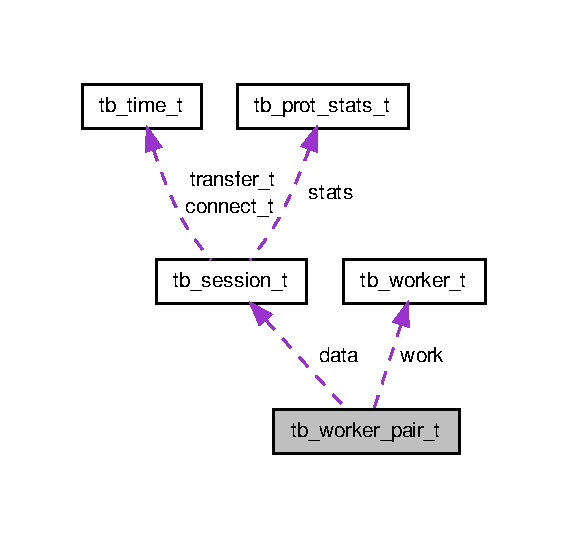
\includegraphics[width=273pt]{structtb__worker__pair__t__coll__graph}
\end{center}
\end{figure}
\subsection*{Data Fields}
\begin{DoxyCompactItemize}
\item 
\hyperlink{structtb__worker__t}{tb\-\_\-worker\-\_\-t} $\ast$ \hyperlink{structtb__worker__pair__t_a251992dcf5d5af0421eb260017a00b2a}{work}
\item 
\hyperlink{structtb__session__t}{tb\-\_\-session\-\_\-t} $\ast$ \hyperlink{structtb__worker__pair__t_a1c1dc2e9642e013fcac80a215230478a}{data}
\end{DoxyCompactItemize}


\subsection{Detailed Description}


Definition at line 15 of file tb\-\_\-worker\-\_\-pair.\-h.



\subsection{Field Documentation}
\hypertarget{structtb__worker__pair__t_a1c1dc2e9642e013fcac80a215230478a}{\index{tb\-\_\-worker\-\_\-pair\-\_\-t@{tb\-\_\-worker\-\_\-pair\-\_\-t}!data@{data}}
\index{data@{data}!tb_worker_pair_t@{tb\-\_\-worker\-\_\-pair\-\_\-t}}
\subsubsection[{data}]{\setlength{\rightskip}{0pt plus 5cm}{\bf tb\-\_\-session\-\_\-t}$\ast$ data}}\label{structtb__worker__pair__t_a1c1dc2e9642e013fcac80a215230478a}


Definition at line 17 of file tb\-\_\-worker\-\_\-pair.\-h.

\hypertarget{structtb__worker__pair__t_a251992dcf5d5af0421eb260017a00b2a}{\index{tb\-\_\-worker\-\_\-pair\-\_\-t@{tb\-\_\-worker\-\_\-pair\-\_\-t}!work@{work}}
\index{work@{work}!tb_worker_pair_t@{tb\-\_\-worker\-\_\-pair\-\_\-t}}
\subsubsection[{work}]{\setlength{\rightskip}{0pt plus 5cm}{\bf tb\-\_\-worker\-\_\-t}$\ast$ work}}\label{structtb__worker__pair__t_a251992dcf5d5af0421eb260017a00b2a}


Definition at line 16 of file tb\-\_\-worker\-\_\-pair.\-h.



The documentation for this struct was generated from the following file\-:\begin{DoxyCompactItemize}
\item 
src/\hyperlink{tb__worker__pair_8h}{tb\-\_\-worker\-\_\-pair.\-h}\end{DoxyCompactItemize}

\hypertarget{structtb__worker__t}{\section{tb\-\_\-worker\-\_\-t Struct Reference}
\label{structtb__worker__t}\index{tb\-\_\-worker\-\_\-t@{tb\-\_\-worker\-\_\-t}}
}


struct that defines fields for worker.  




{\ttfamily \#include $<$tb\-\_\-worker.\-h$>$}

\subsection*{Data Fields}
\begin{DoxyCompactItemize}
\item 
int \hyperlink{structtb__worker__t_a4b75564f2d4bac6720918785d0de5034}{\-\_\-\-\_\-id}
\begin{DoxyCompactList}\small\item\em The unique id of this worker. \end{DoxyCompactList}\item 
gdsl\-\_\-queue\-\_\-t \hyperlink{structtb__worker__t_aea4c15677ebae0f50f9f4684804d7987}{\-\_\-\-\_\-queue}
\begin{DoxyCompactList}\small\item\em The work for this worker. \end{DoxyCompactList}\item 
pthread\-\_\-mutex\-\_\-t $\ast$ \hyperlink{structtb__worker__t_a0721617bd4bf8c42313acd1791f62885}{\-\_\-\-\_\-queue\-\_\-lock}
\begin{DoxyCompactList}\small\item\em The lock for the queue. \end{DoxyCompactList}\item 
pthread\-\_\-cond\-\_\-t $\ast$ \hyperlink{structtb__worker__t_a1302209e4d7c2a7707bfcd735ead74e0}{\-\_\-\-\_\-queue\-\_\-cond}
\begin{DoxyCompactList}\small\item\em The condition for the queue. \end{DoxyCompactList}\item 
int \hyperlink{structtb__worker__t_a3c8ddb573339a9677d54ba3e63387f1d}{\-\_\-\-\_\-stop}
\begin{DoxyCompactList}\small\item\em Stops the thread, 0 to continue, 1 to stop. \end{DoxyCompactList}\end{DoxyCompactItemize}


\subsection{Detailed Description}
struct that defines fields for worker. 

\hyperlink{tb__worker_8h}{tb\-\_\-worker.\-h}

Created on\-: 20/11/2013 Author\-: Michael Holmwood\-This struct defines the fields for class tb\-\_\-worker. The queue contains new work for the worker. The queue\-\_\-lock is used to make the queue thread safe. The worker will sleep if the work queue is empty. Newly added work wakes the thread up using the queue\-\_\-cond. 

Definition at line 25 of file tb\-\_\-worker.\-h.



\subsection{Field Documentation}
\hypertarget{structtb__worker__t_a4b75564f2d4bac6720918785d0de5034}{\index{tb\-\_\-worker\-\_\-t@{tb\-\_\-worker\-\_\-t}!\-\_\-\-\_\-id@{\-\_\-\-\_\-id}}
\index{\-\_\-\-\_\-id@{\-\_\-\-\_\-id}!tb_worker_t@{tb\-\_\-worker\-\_\-t}}
\subsubsection[{\-\_\-\-\_\-id}]{\setlength{\rightskip}{0pt plus 5cm}int \-\_\-\-\_\-id}}\label{structtb__worker__t_a4b75564f2d4bac6720918785d0de5034}


The unique id of this worker. 



Definition at line 27 of file tb\-\_\-worker.\-h.

\hypertarget{structtb__worker__t_aea4c15677ebae0f50f9f4684804d7987}{\index{tb\-\_\-worker\-\_\-t@{tb\-\_\-worker\-\_\-t}!\-\_\-\-\_\-queue@{\-\_\-\-\_\-queue}}
\index{\-\_\-\-\_\-queue@{\-\_\-\-\_\-queue}!tb_worker_t@{tb\-\_\-worker\-\_\-t}}
\subsubsection[{\-\_\-\-\_\-queue}]{\setlength{\rightskip}{0pt plus 5cm}gdsl\-\_\-queue\-\_\-t \-\_\-\-\_\-queue}}\label{structtb__worker__t_aea4c15677ebae0f50f9f4684804d7987}


The work for this worker. 



Definition at line 28 of file tb\-\_\-worker.\-h.

\hypertarget{structtb__worker__t_a1302209e4d7c2a7707bfcd735ead74e0}{\index{tb\-\_\-worker\-\_\-t@{tb\-\_\-worker\-\_\-t}!\-\_\-\-\_\-queue\-\_\-cond@{\-\_\-\-\_\-queue\-\_\-cond}}
\index{\-\_\-\-\_\-queue\-\_\-cond@{\-\_\-\-\_\-queue\-\_\-cond}!tb_worker_t@{tb\-\_\-worker\-\_\-t}}
\subsubsection[{\-\_\-\-\_\-queue\-\_\-cond}]{\setlength{\rightskip}{0pt plus 5cm}pthread\-\_\-cond\-\_\-t$\ast$ \-\_\-\-\_\-queue\-\_\-cond}}\label{structtb__worker__t_a1302209e4d7c2a7707bfcd735ead74e0}


The condition for the queue. 



Definition at line 30 of file tb\-\_\-worker.\-h.

\hypertarget{structtb__worker__t_a0721617bd4bf8c42313acd1791f62885}{\index{tb\-\_\-worker\-\_\-t@{tb\-\_\-worker\-\_\-t}!\-\_\-\-\_\-queue\-\_\-lock@{\-\_\-\-\_\-queue\-\_\-lock}}
\index{\-\_\-\-\_\-queue\-\_\-lock@{\-\_\-\-\_\-queue\-\_\-lock}!tb_worker_t@{tb\-\_\-worker\-\_\-t}}
\subsubsection[{\-\_\-\-\_\-queue\-\_\-lock}]{\setlength{\rightskip}{0pt plus 5cm}pthread\-\_\-mutex\-\_\-t$\ast$ \-\_\-\-\_\-queue\-\_\-lock}}\label{structtb__worker__t_a0721617bd4bf8c42313acd1791f62885}


The lock for the queue. 



Definition at line 29 of file tb\-\_\-worker.\-h.

\hypertarget{structtb__worker__t_a3c8ddb573339a9677d54ba3e63387f1d}{\index{tb\-\_\-worker\-\_\-t@{tb\-\_\-worker\-\_\-t}!\-\_\-\-\_\-stop@{\-\_\-\-\_\-stop}}
\index{\-\_\-\-\_\-stop@{\-\_\-\-\_\-stop}!tb_worker_t@{tb\-\_\-worker\-\_\-t}}
\subsubsection[{\-\_\-\-\_\-stop}]{\setlength{\rightskip}{0pt plus 5cm}int \-\_\-\-\_\-stop}}\label{structtb__worker__t_a3c8ddb573339a9677d54ba3e63387f1d}


Stops the thread, 0 to continue, 1 to stop. 



Definition at line 31 of file tb\-\_\-worker.\-h.



The documentation for this struct was generated from the following file\-:\begin{DoxyCompactItemize}
\item 
src/\hyperlink{tb__worker_8h}{tb\-\_\-worker.\-h}\end{DoxyCompactItemize}

\chapter{File Documentation}
\hypertarget{tb__common_8c}{\section{src/tb\-\_\-common.c File Reference}
\label{tb__common_8c}\index{src/tb\-\_\-common.\-c@{src/tb\-\_\-common.\-c}}
}
{\ttfamily \#include \char`\"{}tb\-\_\-common.\-h\char`\"{}}\\*
{\ttfamily \#include $<$sys/socket.\-h$>$}\\*
{\ttfamily \#include $<$stdio.\-h$>$}\\*
{\ttfamily \#include $<$stdlib.\-h$>$}\\*
{\ttfamily \#include $<$netinet/in.\-h$>$}\\*
{\ttfamily \#include $<$arpa/inet.\-h$>$}\\*
{\ttfamily \#include $<$time.\-h$>$}\\*
{\ttfamily \#include $<$errno.\-h$>$}\\*
Include dependency graph for tb\-\_\-common.\-c\-:\nopagebreak
\begin{figure}[H]
\begin{center}
\leavevmode
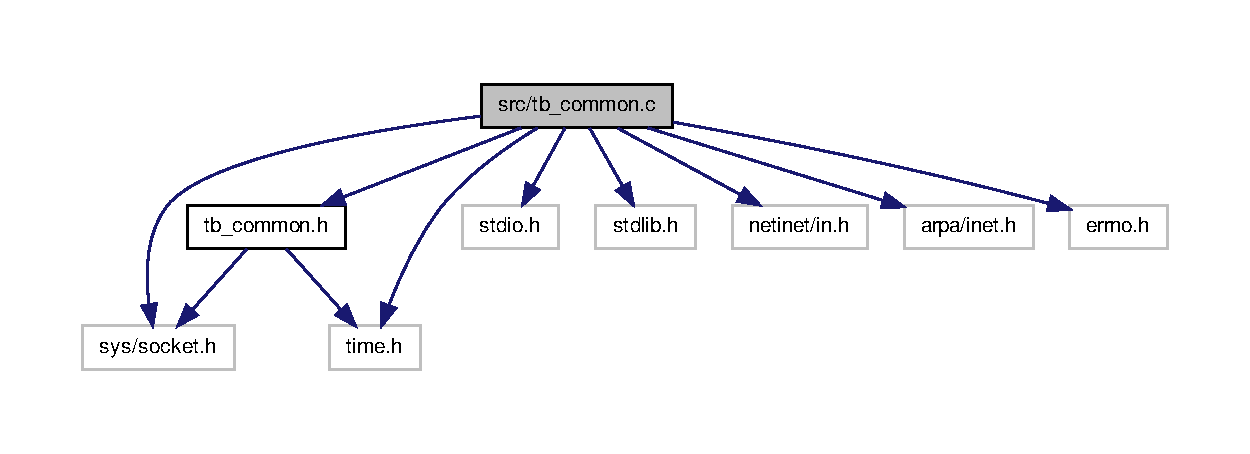
\includegraphics[width=350pt]{tb__common_8c__incl}
\end{center}
\end{figure}
\subsection*{Functions}
\begin{DoxyCompactItemize}
\item 
void \hyperlink{tb__common_8c_a552a8fe72390cc6c07aaa8af6b71f149}{tb\-\_\-print\-\_\-address} (struct sockaddr\-\_\-storage $\ast$store)
\item 
char $\ast$ \hyperlink{tb__common_8c_aa5572e6039ea29b3bfbe1ad5401880e1}{tb\-\_\-get\-\_\-address} (struct sockaddr\-\_\-storage $\ast$store)
\item 
\hyperlink{structtb__time__t}{tb\-\_\-time\-\_\-t} $\ast$ \hyperlink{tb__common_8c_ad9263dd27af44435dbdcf5519c37e39b}{tb\-\_\-create\-\_\-time} (clockid\-\_\-t clk\-\_\-id)
\begin{DoxyCompactList}\small\item\em Create a time struct. \end{DoxyCompactList}\item 
void \hyperlink{tb__common_8c_a9f135b42d60c057bd14984c24a7cc23d}{tb\-\_\-destroy\-\_\-time} (\hyperlink{structtb__time__t}{tb\-\_\-time\-\_\-t} $\ast$time)
\begin{DoxyCompactList}\small\item\em Destroy a \hyperlink{structtb__time__t}{tb\-\_\-time\-\_\-t} struct. \end{DoxyCompactList}\item 
void \hyperlink{tb__common_8c_a49003910b9587f4e37a8212e321b4580}{tb\-\_\-start\-\_\-time} (\hyperlink{structtb__time__t}{tb\-\_\-time\-\_\-t} $\ast$time)
\begin{DoxyCompactList}\small\item\em Record the start time. \end{DoxyCompactList}\item 
void \hyperlink{tb__common_8c_a600d5e4f03f9d4de5cd6d65e6e5c6792}{tb\-\_\-finish\-\_\-time} (\hyperlink{structtb__time__t}{tb\-\_\-time\-\_\-t} $\ast$time)
\begin{DoxyCompactList}\small\item\em Record the finish time. \end{DoxyCompactList}\item 
void \hyperlink{tb__common_8c_aab0e0bc3ffde8c502abe75ceba107ab3}{tb\-\_\-calculate\-\_\-time} (\hyperlink{structtb__time__t}{tb\-\_\-time\-\_\-t} $\ast$time)
\begin{DoxyCompactList}\small\item\em Calculate the time difference between start and stop. \end{DoxyCompactList}\item 
char $\ast$ \hyperlink{tb__common_8c_a4ec357fc778b479d299cad9e82504cf0}{tb\-\_\-create\-\_\-test\-\_\-file} (char $\ast$file\-\_\-name, int $\ast$file\-\_\-size)
\begin{DoxyCompactList}\small\item\em Load the file to be used for sending using the cilent. \end{DoxyCompactList}\item 
char $\ast$ \hyperlink{tb__common_8c_ae3ab0d3349b13d5f813c89f2eca18bf9}{tb\-\_\-load\-\_\-test\-\_\-file} (char $\ast$file\-\_\-name, int $\ast$file\-\_\-size)
\begin{DoxyCompactList}\small\item\em Load file. \end{DoxyCompactList}\item 
char $\ast$ \hyperlink{tb__common_8c_a32e9f0dbdbebb0e77182590d251c6b16}{tb\-\_\-load\-\_\-random\-\_\-file} (int size)
\begin{DoxyCompactList}\small\item\em Load random file of specified size. \end{DoxyCompactList}\item 
char $\ast$ \hyperlink{tb__common_8c_ac679a827a18628284c3003a2af880749}{tb\-\_\-create\-\_\-random} (char $\ast$path, int size)
\begin{DoxyCompactList}\small\item\em Create a random file. \end{DoxyCompactList}\end{DoxyCompactItemize}


\subsection{Function Documentation}
\hypertarget{tb__common_8c_aab0e0bc3ffde8c502abe75ceba107ab3}{\index{tb\-\_\-common.\-c@{tb\-\_\-common.\-c}!tb\-\_\-calculate\-\_\-time@{tb\-\_\-calculate\-\_\-time}}
\index{tb\-\_\-calculate\-\_\-time@{tb\-\_\-calculate\-\_\-time}!tb_common.c@{tb\-\_\-common.\-c}}
\subsubsection[{tb\-\_\-calculate\-\_\-time}]{\setlength{\rightskip}{0pt plus 5cm}void tb\-\_\-calculate\-\_\-time (
\begin{DoxyParamCaption}
\item[{{\bf tb\-\_\-time\-\_\-t} $\ast$}]{time}
\end{DoxyParamCaption}
)\hspace{0.3cm}{\ttfamily [inline]}}}\label{tb__common_8c_aab0e0bc3ffde8c502abe75ceba107ab3}


Calculate the time difference between start and stop. 



Definition at line 80 of file tb\-\_\-common.\-c.

\hypertarget{tb__common_8c_ac679a827a18628284c3003a2af880749}{\index{tb\-\_\-common.\-c@{tb\-\_\-common.\-c}!tb\-\_\-create\-\_\-random@{tb\-\_\-create\-\_\-random}}
\index{tb\-\_\-create\-\_\-random@{tb\-\_\-create\-\_\-random}!tb_common.c@{tb\-\_\-common.\-c}}
\subsubsection[{tb\-\_\-create\-\_\-random}]{\setlength{\rightskip}{0pt plus 5cm}char$\ast$ tb\-\_\-create\-\_\-random (
\begin{DoxyParamCaption}
\item[{char $\ast$}]{path, }
\item[{int}]{size}
\end{DoxyParamCaption}
)}}\label{tb__common_8c_ac679a827a18628284c3003a2af880749}


Create a random file. 



Definition at line 182 of file tb\-\_\-common.\-c.

\hypertarget{tb__common_8c_a4ec357fc778b479d299cad9e82504cf0}{\index{tb\-\_\-common.\-c@{tb\-\_\-common.\-c}!tb\-\_\-create\-\_\-test\-\_\-file@{tb\-\_\-create\-\_\-test\-\_\-file}}
\index{tb\-\_\-create\-\_\-test\-\_\-file@{tb\-\_\-create\-\_\-test\-\_\-file}!tb_common.c@{tb\-\_\-common.\-c}}
\subsubsection[{tb\-\_\-create\-\_\-test\-\_\-file}]{\setlength{\rightskip}{0pt plus 5cm}char$\ast$ tb\-\_\-create\-\_\-test\-\_\-file (
\begin{DoxyParamCaption}
\item[{char $\ast$}]{file\-\_\-name, }
\item[{int $\ast$}]{file\-\_\-size}
\end{DoxyParamCaption}
)}}\label{tb__common_8c_a4ec357fc778b479d299cad9e82504cf0}


Load the file to be used for sending using the cilent. 


\begin{DoxyParams}{Parameters}
{\em listener} & The listener to create the file for. \\
\hline
\end{DoxyParams}


Definition at line 89 of file tb\-\_\-common.\-c.

\hypertarget{tb__common_8c_ad9263dd27af44435dbdcf5519c37e39b}{\index{tb\-\_\-common.\-c@{tb\-\_\-common.\-c}!tb\-\_\-create\-\_\-time@{tb\-\_\-create\-\_\-time}}
\index{tb\-\_\-create\-\_\-time@{tb\-\_\-create\-\_\-time}!tb_common.c@{tb\-\_\-common.\-c}}
\subsubsection[{tb\-\_\-create\-\_\-time}]{\setlength{\rightskip}{0pt plus 5cm}{\bf tb\-\_\-time\-\_\-t}$\ast$ tb\-\_\-create\-\_\-time (
\begin{DoxyParamCaption}
\item[{clockid\-\_\-t}]{clk\-\_\-id}
\end{DoxyParamCaption}
)}}\label{tb__common_8c_ad9263dd27af44435dbdcf5519c37e39b}


Create a time struct. 


\begin{DoxyParams}{Parameters}
{\em clk\-\_\-id} & The id of the type of clock to use. \\
\hline
\end{DoxyParams}


Definition at line 47 of file tb\-\_\-common.\-c.

\hypertarget{tb__common_8c_a9f135b42d60c057bd14984c24a7cc23d}{\index{tb\-\_\-common.\-c@{tb\-\_\-common.\-c}!tb\-\_\-destroy\-\_\-time@{tb\-\_\-destroy\-\_\-time}}
\index{tb\-\_\-destroy\-\_\-time@{tb\-\_\-destroy\-\_\-time}!tb_common.c@{tb\-\_\-common.\-c}}
\subsubsection[{tb\-\_\-destroy\-\_\-time}]{\setlength{\rightskip}{0pt plus 5cm}void tb\-\_\-destroy\-\_\-time (
\begin{DoxyParamCaption}
\item[{{\bf tb\-\_\-time\-\_\-t} $\ast$}]{time}
\end{DoxyParamCaption}
)}}\label{tb__common_8c_a9f135b42d60c057bd14984c24a7cc23d}


Destroy a \hyperlink{structtb__time__t}{tb\-\_\-time\-\_\-t} struct. 



Definition at line 59 of file tb\-\_\-common.\-c.

\hypertarget{tb__common_8c_a600d5e4f03f9d4de5cd6d65e6e5c6792}{\index{tb\-\_\-common.\-c@{tb\-\_\-common.\-c}!tb\-\_\-finish\-\_\-time@{tb\-\_\-finish\-\_\-time}}
\index{tb\-\_\-finish\-\_\-time@{tb\-\_\-finish\-\_\-time}!tb_common.c@{tb\-\_\-common.\-c}}
\subsubsection[{tb\-\_\-finish\-\_\-time}]{\setlength{\rightskip}{0pt plus 5cm}void tb\-\_\-finish\-\_\-time (
\begin{DoxyParamCaption}
\item[{{\bf tb\-\_\-time\-\_\-t} $\ast$}]{time}
\end{DoxyParamCaption}
)\hspace{0.3cm}{\ttfamily [inline]}}}\label{tb__common_8c_a600d5e4f03f9d4de5cd6d65e6e5c6792}


Record the finish time. 



Definition at line 73 of file tb\-\_\-common.\-c.

\hypertarget{tb__common_8c_aa5572e6039ea29b3bfbe1ad5401880e1}{\index{tb\-\_\-common.\-c@{tb\-\_\-common.\-c}!tb\-\_\-get\-\_\-address@{tb\-\_\-get\-\_\-address}}
\index{tb\-\_\-get\-\_\-address@{tb\-\_\-get\-\_\-address}!tb_common.c@{tb\-\_\-common.\-c}}
\subsubsection[{tb\-\_\-get\-\_\-address}]{\setlength{\rightskip}{0pt plus 5cm}char$\ast$ tb\-\_\-get\-\_\-address (
\begin{DoxyParamCaption}
\item[{struct sockaddr\-\_\-storage $\ast$}]{store}
\end{DoxyParamCaption}
)\hspace{0.3cm}{\ttfamily [inline]}}}\label{tb__common_8c_aa5572e6039ea29b3bfbe1ad5401880e1}


Definition at line 26 of file tb\-\_\-common.\-c.

\hypertarget{tb__common_8c_a32e9f0dbdbebb0e77182590d251c6b16}{\index{tb\-\_\-common.\-c@{tb\-\_\-common.\-c}!tb\-\_\-load\-\_\-random\-\_\-file@{tb\-\_\-load\-\_\-random\-\_\-file}}
\index{tb\-\_\-load\-\_\-random\-\_\-file@{tb\-\_\-load\-\_\-random\-\_\-file}!tb_common.c@{tb\-\_\-common.\-c}}
\subsubsection[{tb\-\_\-load\-\_\-random\-\_\-file}]{\setlength{\rightskip}{0pt plus 5cm}char$\ast$ tb\-\_\-load\-\_\-random\-\_\-file (
\begin{DoxyParamCaption}
\item[{int}]{size}
\end{DoxyParamCaption}
)}}\label{tb__common_8c_a32e9f0dbdbebb0e77182590d251c6b16}


Load random file of specified size. 

Loads a pre-\/generated file of the specified size, or generates it if it does not exist. 

Definition at line 148 of file tb\-\_\-common.\-c.

\hypertarget{tb__common_8c_ae3ab0d3349b13d5f813c89f2eca18bf9}{\index{tb\-\_\-common.\-c@{tb\-\_\-common.\-c}!tb\-\_\-load\-\_\-test\-\_\-file@{tb\-\_\-load\-\_\-test\-\_\-file}}
\index{tb\-\_\-load\-\_\-test\-\_\-file@{tb\-\_\-load\-\_\-test\-\_\-file}!tb_common.c@{tb\-\_\-common.\-c}}
\subsubsection[{tb\-\_\-load\-\_\-test\-\_\-file}]{\setlength{\rightskip}{0pt plus 5cm}char$\ast$ tb\-\_\-load\-\_\-test\-\_\-file (
\begin{DoxyParamCaption}
\item[{char $\ast$}]{file\-\_\-name, }
\item[{int $\ast$}]{file\-\_\-size}
\end{DoxyParamCaption}
)}}\label{tb__common_8c_ae3ab0d3349b13d5f813c89f2eca18bf9}


Load file. 



Definition at line 118 of file tb\-\_\-common.\-c.

\hypertarget{tb__common_8c_a552a8fe72390cc6c07aaa8af6b71f149}{\index{tb\-\_\-common.\-c@{tb\-\_\-common.\-c}!tb\-\_\-print\-\_\-address@{tb\-\_\-print\-\_\-address}}
\index{tb\-\_\-print\-\_\-address@{tb\-\_\-print\-\_\-address}!tb_common.c@{tb\-\_\-common.\-c}}
\subsubsection[{tb\-\_\-print\-\_\-address}]{\setlength{\rightskip}{0pt plus 5cm}void tb\-\_\-print\-\_\-address (
\begin{DoxyParamCaption}
\item[{struct sockaddr\-\_\-storage $\ast$}]{store}
\end{DoxyParamCaption}
)\hspace{0.3cm}{\ttfamily [inline]}}}\label{tb__common_8c_a552a8fe72390cc6c07aaa8af6b71f149}


Definition at line 18 of file tb\-\_\-common.\-c.

\hypertarget{tb__common_8c_a49003910b9587f4e37a8212e321b4580}{\index{tb\-\_\-common.\-c@{tb\-\_\-common.\-c}!tb\-\_\-start\-\_\-time@{tb\-\_\-start\-\_\-time}}
\index{tb\-\_\-start\-\_\-time@{tb\-\_\-start\-\_\-time}!tb_common.c@{tb\-\_\-common.\-c}}
\subsubsection[{tb\-\_\-start\-\_\-time}]{\setlength{\rightskip}{0pt plus 5cm}void tb\-\_\-start\-\_\-time (
\begin{DoxyParamCaption}
\item[{{\bf tb\-\_\-time\-\_\-t} $\ast$}]{time}
\end{DoxyParamCaption}
)\hspace{0.3cm}{\ttfamily [inline]}}}\label{tb__common_8c_a49003910b9587f4e37a8212e321b4580}


Record the start time. 



Definition at line 67 of file tb\-\_\-common.\-c.


\hypertarget{tb__common_8h}{\section{src/tb\-\_\-common.h File Reference}
\label{tb__common_8h}\index{src/tb\-\_\-common.\-h@{src/tb\-\_\-common.\-h}}
}
{\ttfamily \#include $<$sys/socket.\-h$>$}\\*
{\ttfamily \#include $<$time.\-h$>$}\\*
Include dependency graph for tb\-\_\-common.\-h\-:\nopagebreak
\begin{figure}[H]
\begin{center}
\leavevmode
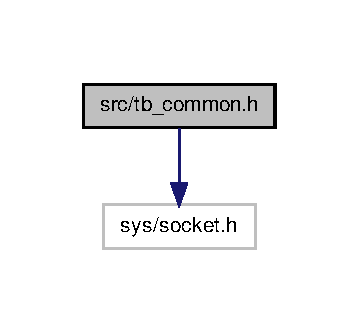
\includegraphics[width=172pt]{tb__common_8h__incl}
\end{center}
\end{figure}
This graph shows which files directly or indirectly include this file\-:\nopagebreak
\begin{figure}[H]
\begin{center}
\leavevmode
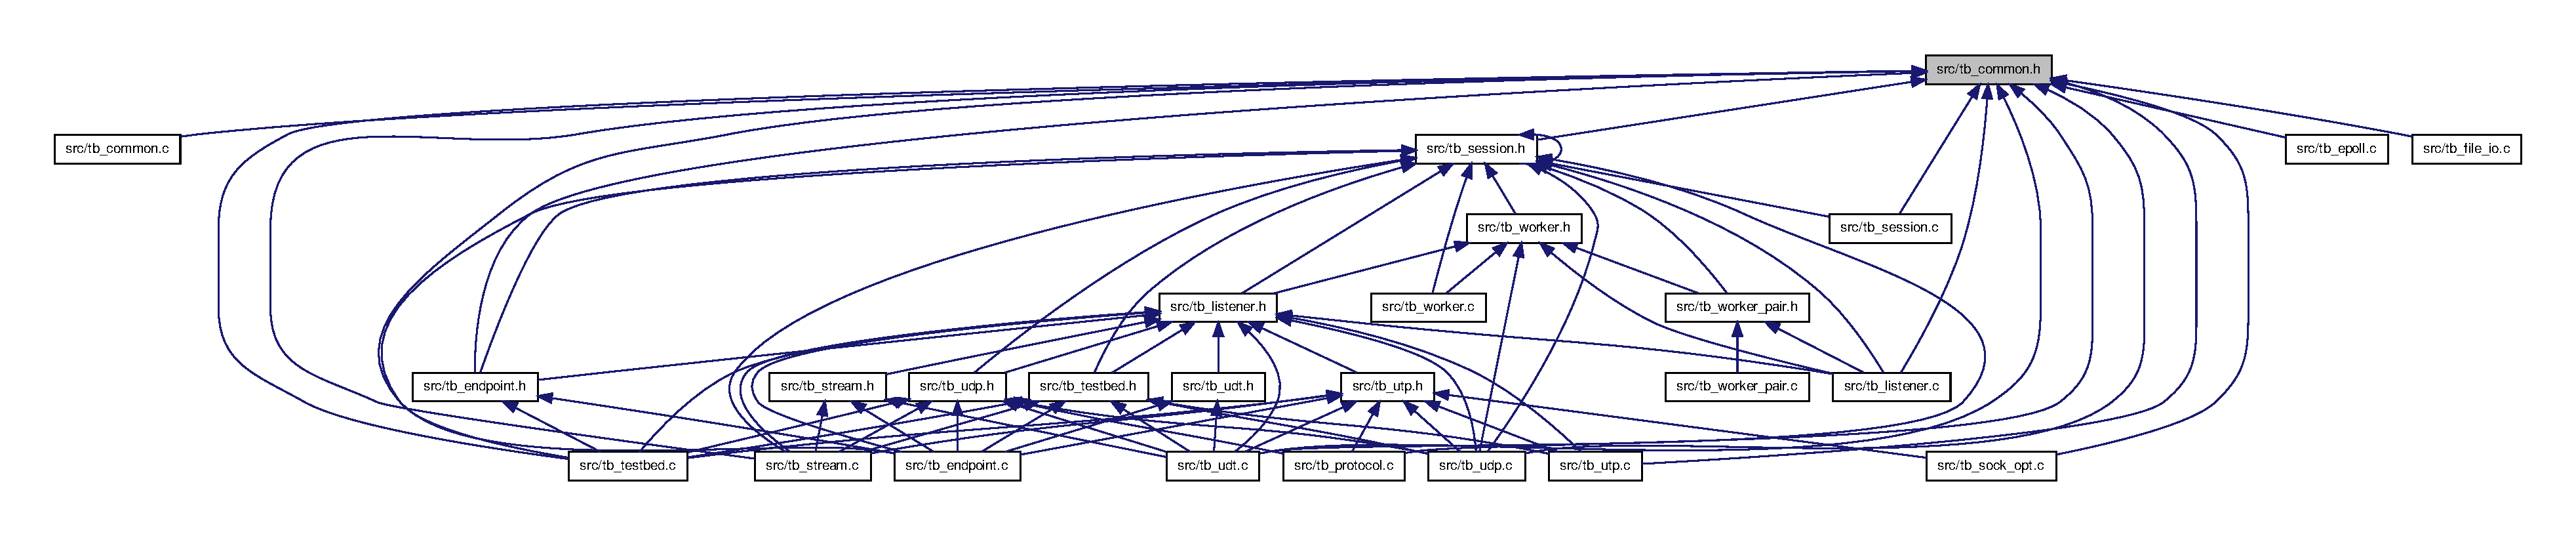
\includegraphics[width=350pt]{tb__common_8h__dep__incl}
\end{center}
\end{figure}
\subsection*{Data Structures}
\begin{DoxyCompactItemize}
\item 
struct \hyperlink{structtb__time__t}{tb\-\_\-time\-\_\-t}
\begin{DoxyCompactList}\small\item\em A struct to hold start, stop and elapsed times. \end{DoxyCompactList}\end{DoxyCompactItemize}
\subsection*{Macros}
\begin{DoxyCompactItemize}
\item 
\#define \hyperlink{tb__common_8h_a7b3b25cba33b07c303f3060fe41887f6}{B\-L\-A\-C\-K}~\char`\"{}\textbackslash{}x1b\mbox{[}22;30m\char`\"{}
\item 
\#define \hyperlink{tb__common_8h_a8d23feea868a983c8c2b661e1e16972f}{R\-E\-D}~\char`\"{}\textbackslash{}x1b\mbox{[}22;31m\char`\"{}
\item 
\#define \hyperlink{tb__common_8h_acfbc006ea433ad708fdee3e82996e721}{G\-R\-E\-E\-N}~\char`\"{}\textbackslash{}x1b\mbox{[}22;32m\char`\"{}
\item 
\#define \hyperlink{tb__common_8h_a79d10e672abb49ad63eeaa8aaef57c38}{B\-L\-U\-E}~\char`\"{}\textbackslash{}x1b\mbox{[}22;34m\char`\"{}
\item 
\#define \hyperlink{tb__common_8h_ab702106cf3b3e96750b6845ded4e0299}{R\-E\-S\-E\-T}~\char`\"{}\textbackslash{}x1b\mbox{[}39m\char`\"{}
\item 
\#define \hyperlink{tb__common_8h_a611cc9b5f655508482f3d7a9751c182a}{C\-L\-E\-A\-R}~\char`\"{}\textbackslash{}x1b\mbox{[}2\-J\char`\"{}
\item 
\#define \hyperlink{tb__common_8h_af94cfb03461685fead1fe045d5c96f01}{L\-I\-N\-E}~\char`\"{}\textbackslash{}n===================================\textbackslash{}n\char`\"{}
\item 
\#define \hyperlink{tb__common_8h_a5b45f1cb2a058dd5df8541b31cb4a5b0}{M\-O\-V\-E\-\_\-\-C\-S\-R}(n, m)~\char`\"{}\textbackslash{}x1b\mbox{[}\char`\"{} \#n \char`\"{};\char`\"{} \#m \char`\"{}H\char`\"{}
\item 
\#define \hyperlink{tb__common_8h_a77cccdd506f431925643040baa01e4e0}{A\-C\-K}(str)~\hyperlink{tb__common_8h_acfbc006ea433ad708fdee3e82996e721}{G\-R\-E\-E\-N} str \hyperlink{tb__common_8h_ab702106cf3b3e96750b6845ded4e0299}{R\-E\-S\-E\-T}
\item 
\#define \hyperlink{tb__common_8h_abd591efbd24cc8f766bb57b5e2847739}{E\-R\-R}(str)~\hyperlink{tb__common_8h_a8d23feea868a983c8c2b661e1e16972f}{R\-E\-D} str \hyperlink{tb__common_8h_ab702106cf3b3e96750b6845ded4e0299}{R\-E\-S\-E\-T}
\item 
\#define \hyperlink{tb__common_8h_a1482e48c7a5fd002739cc9b33f1a292d}{I\-N\-F\-O}(str)~\hyperlink{tb__common_8h_a79d10e672abb49ad63eeaa8aaef57c38}{B\-L\-U\-E} str \hyperlink{tb__common_8h_ab702106cf3b3e96750b6845ded4e0299}{R\-E\-S\-E\-T}
\item 
\#define \hyperlink{tb__common_8h_a06e3a3123fb05c14a8240e56817ca0da}{P\-R\-T\-\_\-\-E\-R\-R}(str)~fprintf(stderr, \hyperlink{tb__common_8h_abd591efbd24cc8f766bb57b5e2847739}{E\-R\-R}(str) \char`\"{}\textbackslash{}n\char`\"{})
\item 
\#define \hyperlink{tb__common_8h_a115c55d70575a04bcd4c5b25c664e4df}{P\-R\-T\-\_\-\-A\-C\-K}(str)~fprintf(stdout, \hyperlink{tb__common_8h_a77cccdd506f431925643040baa01e4e0}{A\-C\-K}(str) \char`\"{}\textbackslash{}n\char`\"{})
\item 
\#define \hyperlink{tb__common_8h_a189cd5397305bc0da38f767312901e6b}{P\-R\-T\-\_\-\-I\-N\-F\-O}(str)~fprintf(stdout, \hyperlink{tb__common_8h_a1482e48c7a5fd002739cc9b33f1a292d}{I\-N\-F\-O}(str) \char`\"{}\textbackslash{}n\char`\"{})
\item 
\#define \hyperlink{tb__common_8h_a52097ccd0cd25faadb3949cab6cf2e4c}{P\-R\-T\-\_\-\-E\-R\-R\-\_\-\-P\-A\-R\-A\-M}(str, mod, param)~fprintf(stderr, \hyperlink{tb__common_8h_a77cccdd506f431925643040baa01e4e0}{A\-C\-K}(str)mod, param)
\item 
\#define \hyperlink{tb__common_8h_a851f14084bc2c7455254cfc03a4ffde5}{P\-R\-T\-\_\-\-I\-\_\-\-D}(str, num)~fprintf(stdout, \hyperlink{tb__common_8h_a1482e48c7a5fd002739cc9b33f1a292d}{I\-N\-F\-O}(str) \char`\"{}\textbackslash{}n\char`\"{}, num)
\item 
\#define \hyperlink{tb__common_8h_a799a3082c570c7896f84c7289c951048}{P\-R\-T\-\_\-\-I\-\_\-\-S}(str, s)~fprintf(stdout, \hyperlink{tb__common_8h_a1482e48c7a5fd002739cc9b33f1a292d}{I\-N\-F\-O}(str) \char`\"{}\-:\%s\textbackslash{}n\char`\"{}, s)
\item 
\#define \hyperlink{tb__common_8h_a86fb58f67f598a20528cfda8e449197a}{P\-R\-T\-\_\-\-E\-\_\-\-S}(str, s)~fprintf(stdout, \hyperlink{tb__common_8h_abd591efbd24cc8f766bb57b5e2847739}{E\-R\-R}(str) \char`\"{}\-:\%s\char`\"{}, s)
\item 
\#define \hyperlink{tb__common_8h_a35b0ee3a629b1f09562640dd8b296c4a}{L\-O\-G}(l, i, t)~if(l-\/$>$log\-\_\-enabled) \hyperlink{tb__logging_8h_a82ad705fd902df959659c7460c4d10b9}{tb\-\_\-write\-\_\-log}(l-\/$>$log\-\_\-info, i, t)
\item 
\#define \hyperlink{tb__common_8h_a28ada5a2f9e41a5bd6855785f0726bd3}{L\-O\-G\-\_\-\-E\-R\-R}(l, i)~\hyperlink{tb__common_8h_a06e3a3123fb05c14a8240e56817ca0da}{P\-R\-T\-\_\-\-E\-R\-R}(i) if(l-\/$>$log\-\_\-enabled) \hyperlink{tb__logging_8h_a82ad705fd902df959659c7460c4d10b9}{tb\-\_\-write\-\_\-log}(l-\/$>$log\-\_\-info, i, t)
\item 
\#define \hyperlink{tb__common_8h_a873febb42fd9613b2b83b457612a2a06}{L\-O\-G\-\_\-\-A\-D\-D}(l, i, s)~if(l-\/$>$log\-\_\-enabled) \hyperlink{tb__listener_8h_ae35166dd784547cfb9d71a3b9af3dd2b}{tb\-\_\-address}(l, i, s)
\end{DoxyCompactItemize}
\subsection*{Functions}
\begin{DoxyCompactItemize}
\item 
void \hyperlink{tb__common_8h_a173bdbe188f1db7efceac0a9a2aa234a}{tb\-\_\-print\-\_\-address} (struct sockaddr\-\_\-storage $\ast$store) \-\_\-\-\_\-attribute\-\_\-\-\_\-((always\-\_\-inline))
\item 
char $\ast$ \hyperlink{tb__common_8h_a26189e2b0857c949ab5770bb71b937a4}{tb\-\_\-get\-\_\-address} (struct sockaddr\-\_\-storage $\ast$store) \-\_\-\-\_\-attribute\-\_\-\-\_\-((always\-\_\-inline))
\item 
\hyperlink{structtb__time__t}{tb\-\_\-time\-\_\-t} $\ast$ \hyperlink{tb__common_8h_ad9263dd27af44435dbdcf5519c37e39b}{tb\-\_\-create\-\_\-time} (clockid\-\_\-t clk\-\_\-id)
\begin{DoxyCompactList}\small\item\em Create a time struct. \end{DoxyCompactList}\item 
void \hyperlink{tb__common_8h_a9f135b42d60c057bd14984c24a7cc23d}{tb\-\_\-destroy\-\_\-time} (\hyperlink{structtb__time__t}{tb\-\_\-time\-\_\-t} $\ast$time)
\begin{DoxyCompactList}\small\item\em Destroy a \hyperlink{structtb__time__t}{tb\-\_\-time\-\_\-t} struct. \end{DoxyCompactList}\item 
void \hyperlink{tb__common_8h_ae97b949920c7200bad9a3b31a3c533fc}{tb\-\_\-start\-\_\-time} (\hyperlink{structtb__time__t}{tb\-\_\-time\-\_\-t} $\ast$time) \-\_\-\-\_\-attribute\-\_\-\-\_\-((always\-\_\-inline))
\begin{DoxyCompactList}\small\item\em Record the start time. \end{DoxyCompactList}\item 
void \hyperlink{tb__common_8h_a9640c3df780843268a2a6979e2d84930}{tb\-\_\-finish\-\_\-time} (\hyperlink{structtb__time__t}{tb\-\_\-time\-\_\-t} $\ast$time) \-\_\-\-\_\-attribute\-\_\-\-\_\-((always\-\_\-inline))
\begin{DoxyCompactList}\small\item\em Record the finish time. \end{DoxyCompactList}\item 
void \hyperlink{tb__common_8h_aff11bd60fd34291672f93803416b1139}{tb\-\_\-calculate\-\_\-time} (\hyperlink{structtb__time__t}{tb\-\_\-time\-\_\-t} $\ast$time) \-\_\-\-\_\-attribute\-\_\-\-\_\-((always\-\_\-inline))
\begin{DoxyCompactList}\small\item\em Calculate the time difference between start and stop. \end{DoxyCompactList}\item 
char $\ast$ \hyperlink{tb__common_8h_a4ec357fc778b479d299cad9e82504cf0}{tb\-\_\-create\-\_\-test\-\_\-file} (char $\ast$file\-\_\-name, int $\ast$file\-\_\-size)
\begin{DoxyCompactList}\small\item\em Load the file to be used for sending using the cilent. \end{DoxyCompactList}\item 
char $\ast$ \hyperlink{tb__common_8h_ae3ab0d3349b13d5f813c89f2eca18bf9}{tb\-\_\-load\-\_\-test\-\_\-file} (char $\ast$file\-\_\-name, int $\ast$file\-\_\-size)
\begin{DoxyCompactList}\small\item\em Load file. \end{DoxyCompactList}\item 
char $\ast$ \hyperlink{tb__common_8h_a32e9f0dbdbebb0e77182590d251c6b16}{tb\-\_\-load\-\_\-random\-\_\-file} (int size)
\begin{DoxyCompactList}\small\item\em Load random file of specified size. \end{DoxyCompactList}\item 
char $\ast$ \hyperlink{tb__common_8h_ac679a827a18628284c3003a2af880749}{tb\-\_\-create\-\_\-random} (char $\ast$path, int size)
\begin{DoxyCompactList}\small\item\em Create a random file. \end{DoxyCompactList}\end{DoxyCompactItemize}


\subsection{Macro Definition Documentation}
\hypertarget{tb__common_8h_a77cccdd506f431925643040baa01e4e0}{\index{tb\-\_\-common.\-h@{tb\-\_\-common.\-h}!A\-C\-K@{A\-C\-K}}
\index{A\-C\-K@{A\-C\-K}!tb_common.h@{tb\-\_\-common.\-h}}
\subsubsection[{A\-C\-K}]{\setlength{\rightskip}{0pt plus 5cm}\#define A\-C\-K(
\begin{DoxyParamCaption}
\item[{}]{str}
\end{DoxyParamCaption}
)~{\bf G\-R\-E\-E\-N} str {\bf R\-E\-S\-E\-T}}}\label{tb__common_8h_a77cccdd506f431925643040baa01e4e0}


Definition at line 22 of file tb\-\_\-common.\-h.

\hypertarget{tb__common_8h_a7b3b25cba33b07c303f3060fe41887f6}{\index{tb\-\_\-common.\-h@{tb\-\_\-common.\-h}!B\-L\-A\-C\-K@{B\-L\-A\-C\-K}}
\index{B\-L\-A\-C\-K@{B\-L\-A\-C\-K}!tb_common.h@{tb\-\_\-common.\-h}}
\subsubsection[{B\-L\-A\-C\-K}]{\setlength{\rightskip}{0pt plus 5cm}\#define B\-L\-A\-C\-K~\char`\"{}\textbackslash{}x1b\mbox{[}22;30m\char`\"{}}}\label{tb__common_8h_a7b3b25cba33b07c303f3060fe41887f6}


Definition at line 14 of file tb\-\_\-common.\-h.

\hypertarget{tb__common_8h_a79d10e672abb49ad63eeaa8aaef57c38}{\index{tb\-\_\-common.\-h@{tb\-\_\-common.\-h}!B\-L\-U\-E@{B\-L\-U\-E}}
\index{B\-L\-U\-E@{B\-L\-U\-E}!tb_common.h@{tb\-\_\-common.\-h}}
\subsubsection[{B\-L\-U\-E}]{\setlength{\rightskip}{0pt plus 5cm}\#define B\-L\-U\-E~\char`\"{}\textbackslash{}x1b\mbox{[}22;34m\char`\"{}}}\label{tb__common_8h_a79d10e672abb49ad63eeaa8aaef57c38}


Definition at line 17 of file tb\-\_\-common.\-h.

\hypertarget{tb__common_8h_a611cc9b5f655508482f3d7a9751c182a}{\index{tb\-\_\-common.\-h@{tb\-\_\-common.\-h}!C\-L\-E\-A\-R@{C\-L\-E\-A\-R}}
\index{C\-L\-E\-A\-R@{C\-L\-E\-A\-R}!tb_common.h@{tb\-\_\-common.\-h}}
\subsubsection[{C\-L\-E\-A\-R}]{\setlength{\rightskip}{0pt plus 5cm}\#define C\-L\-E\-A\-R~\char`\"{}\textbackslash{}x1b\mbox{[}2\-J\char`\"{}}}\label{tb__common_8h_a611cc9b5f655508482f3d7a9751c182a}


Definition at line 19 of file tb\-\_\-common.\-h.

\hypertarget{tb__common_8h_abd591efbd24cc8f766bb57b5e2847739}{\index{tb\-\_\-common.\-h@{tb\-\_\-common.\-h}!E\-R\-R@{E\-R\-R}}
\index{E\-R\-R@{E\-R\-R}!tb_common.h@{tb\-\_\-common.\-h}}
\subsubsection[{E\-R\-R}]{\setlength{\rightskip}{0pt plus 5cm}\#define E\-R\-R(
\begin{DoxyParamCaption}
\item[{}]{str}
\end{DoxyParamCaption}
)~{\bf R\-E\-D} str {\bf R\-E\-S\-E\-T}}}\label{tb__common_8h_abd591efbd24cc8f766bb57b5e2847739}


Definition at line 23 of file tb\-\_\-common.\-h.

\hypertarget{tb__common_8h_acfbc006ea433ad708fdee3e82996e721}{\index{tb\-\_\-common.\-h@{tb\-\_\-common.\-h}!G\-R\-E\-E\-N@{G\-R\-E\-E\-N}}
\index{G\-R\-E\-E\-N@{G\-R\-E\-E\-N}!tb_common.h@{tb\-\_\-common.\-h}}
\subsubsection[{G\-R\-E\-E\-N}]{\setlength{\rightskip}{0pt plus 5cm}\#define G\-R\-E\-E\-N~\char`\"{}\textbackslash{}x1b\mbox{[}22;32m\char`\"{}}}\label{tb__common_8h_acfbc006ea433ad708fdee3e82996e721}


Definition at line 16 of file tb\-\_\-common.\-h.

\hypertarget{tb__common_8h_a1482e48c7a5fd002739cc9b33f1a292d}{\index{tb\-\_\-common.\-h@{tb\-\_\-common.\-h}!I\-N\-F\-O@{I\-N\-F\-O}}
\index{I\-N\-F\-O@{I\-N\-F\-O}!tb_common.h@{tb\-\_\-common.\-h}}
\subsubsection[{I\-N\-F\-O}]{\setlength{\rightskip}{0pt plus 5cm}\#define I\-N\-F\-O(
\begin{DoxyParamCaption}
\item[{}]{str}
\end{DoxyParamCaption}
)~{\bf B\-L\-U\-E} str {\bf R\-E\-S\-E\-T}}}\label{tb__common_8h_a1482e48c7a5fd002739cc9b33f1a292d}


Definition at line 24 of file tb\-\_\-common.\-h.

\hypertarget{tb__common_8h_af94cfb03461685fead1fe045d5c96f01}{\index{tb\-\_\-common.\-h@{tb\-\_\-common.\-h}!L\-I\-N\-E@{L\-I\-N\-E}}
\index{L\-I\-N\-E@{L\-I\-N\-E}!tb_common.h@{tb\-\_\-common.\-h}}
\subsubsection[{L\-I\-N\-E}]{\setlength{\rightskip}{0pt plus 5cm}\#define L\-I\-N\-E~\char`\"{}\textbackslash{}n===================================\textbackslash{}n\char`\"{}}}\label{tb__common_8h_af94cfb03461685fead1fe045d5c96f01}


Definition at line 20 of file tb\-\_\-common.\-h.

\hypertarget{tb__common_8h_a35b0ee3a629b1f09562640dd8b296c4a}{\index{tb\-\_\-common.\-h@{tb\-\_\-common.\-h}!L\-O\-G@{L\-O\-G}}
\index{L\-O\-G@{L\-O\-G}!tb_common.h@{tb\-\_\-common.\-h}}
\subsubsection[{L\-O\-G}]{\setlength{\rightskip}{0pt plus 5cm}\#define L\-O\-G(
\begin{DoxyParamCaption}
\item[{}]{l, }
\item[{}]{i, }
\item[{}]{t}
\end{DoxyParamCaption}
)~if(l-\/$>$log\-\_\-enabled) {\bf tb\-\_\-write\-\_\-log}(l-\/$>$log\-\_\-info, i, t)}}\label{tb__common_8h_a35b0ee3a629b1f09562640dd8b296c4a}


Definition at line 33 of file tb\-\_\-common.\-h.

\hypertarget{tb__common_8h_a873febb42fd9613b2b83b457612a2a06}{\index{tb\-\_\-common.\-h@{tb\-\_\-common.\-h}!L\-O\-G\-\_\-\-A\-D\-D@{L\-O\-G\-\_\-\-A\-D\-D}}
\index{L\-O\-G\-\_\-\-A\-D\-D@{L\-O\-G\-\_\-\-A\-D\-D}!tb_common.h@{tb\-\_\-common.\-h}}
\subsubsection[{L\-O\-G\-\_\-\-A\-D\-D}]{\setlength{\rightskip}{0pt plus 5cm}\#define L\-O\-G\-\_\-\-A\-D\-D(
\begin{DoxyParamCaption}
\item[{}]{l, }
\item[{}]{i, }
\item[{}]{s}
\end{DoxyParamCaption}
)~if(l-\/$>$log\-\_\-enabled) {\bf tb\-\_\-address}(l, i, s)}}\label{tb__common_8h_a873febb42fd9613b2b83b457612a2a06}


Definition at line 35 of file tb\-\_\-common.\-h.

\hypertarget{tb__common_8h_a28ada5a2f9e41a5bd6855785f0726bd3}{\index{tb\-\_\-common.\-h@{tb\-\_\-common.\-h}!L\-O\-G\-\_\-\-E\-R\-R@{L\-O\-G\-\_\-\-E\-R\-R}}
\index{L\-O\-G\-\_\-\-E\-R\-R@{L\-O\-G\-\_\-\-E\-R\-R}!tb_common.h@{tb\-\_\-common.\-h}}
\subsubsection[{L\-O\-G\-\_\-\-E\-R\-R}]{\setlength{\rightskip}{0pt plus 5cm}\#define L\-O\-G\-\_\-\-E\-R\-R(
\begin{DoxyParamCaption}
\item[{}]{l, }
\item[{}]{i}
\end{DoxyParamCaption}
)~{\bf P\-R\-T\-\_\-\-E\-R\-R}(i) if(l-\/$>$log\-\_\-enabled) {\bf tb\-\_\-write\-\_\-log}(l-\/$>$log\-\_\-info, i, t)}}\label{tb__common_8h_a28ada5a2f9e41a5bd6855785f0726bd3}


Definition at line 34 of file tb\-\_\-common.\-h.

\hypertarget{tb__common_8h_a5b45f1cb2a058dd5df8541b31cb4a5b0}{\index{tb\-\_\-common.\-h@{tb\-\_\-common.\-h}!M\-O\-V\-E\-\_\-\-C\-S\-R@{M\-O\-V\-E\-\_\-\-C\-S\-R}}
\index{M\-O\-V\-E\-\_\-\-C\-S\-R@{M\-O\-V\-E\-\_\-\-C\-S\-R}!tb_common.h@{tb\-\_\-common.\-h}}
\subsubsection[{M\-O\-V\-E\-\_\-\-C\-S\-R}]{\setlength{\rightskip}{0pt plus 5cm}\#define M\-O\-V\-E\-\_\-\-C\-S\-R(
\begin{DoxyParamCaption}
\item[{}]{n, }
\item[{}]{m}
\end{DoxyParamCaption}
)~\char`\"{}\textbackslash{}x1b\mbox{[}\char`\"{} \#n \char`\"{};\char`\"{} \#m \char`\"{}H\char`\"{}}}\label{tb__common_8h_a5b45f1cb2a058dd5df8541b31cb4a5b0}


Definition at line 21 of file tb\-\_\-common.\-h.

\hypertarget{tb__common_8h_a115c55d70575a04bcd4c5b25c664e4df}{\index{tb\-\_\-common.\-h@{tb\-\_\-common.\-h}!P\-R\-T\-\_\-\-A\-C\-K@{P\-R\-T\-\_\-\-A\-C\-K}}
\index{P\-R\-T\-\_\-\-A\-C\-K@{P\-R\-T\-\_\-\-A\-C\-K}!tb_common.h@{tb\-\_\-common.\-h}}
\subsubsection[{P\-R\-T\-\_\-\-A\-C\-K}]{\setlength{\rightskip}{0pt plus 5cm}\#define P\-R\-T\-\_\-\-A\-C\-K(
\begin{DoxyParamCaption}
\item[{}]{str}
\end{DoxyParamCaption}
)~fprintf(stdout, {\bf A\-C\-K}(str) \char`\"{}\textbackslash{}n\char`\"{})}}\label{tb__common_8h_a115c55d70575a04bcd4c5b25c664e4df}


Definition at line 26 of file tb\-\_\-common.\-h.

\hypertarget{tb__common_8h_a86fb58f67f598a20528cfda8e449197a}{\index{tb\-\_\-common.\-h@{tb\-\_\-common.\-h}!P\-R\-T\-\_\-\-E\-\_\-\-S@{P\-R\-T\-\_\-\-E\-\_\-\-S}}
\index{P\-R\-T\-\_\-\-E\-\_\-\-S@{P\-R\-T\-\_\-\-E\-\_\-\-S}!tb_common.h@{tb\-\_\-common.\-h}}
\subsubsection[{P\-R\-T\-\_\-\-E\-\_\-\-S}]{\setlength{\rightskip}{0pt plus 5cm}\#define P\-R\-T\-\_\-\-E\-\_\-\-S(
\begin{DoxyParamCaption}
\item[{}]{str, }
\item[{}]{s}
\end{DoxyParamCaption}
)~fprintf(stdout, {\bf E\-R\-R}(str) \char`\"{}\-:\%s\char`\"{}, s)}}\label{tb__common_8h_a86fb58f67f598a20528cfda8e449197a}


Definition at line 31 of file tb\-\_\-common.\-h.

\hypertarget{tb__common_8h_a06e3a3123fb05c14a8240e56817ca0da}{\index{tb\-\_\-common.\-h@{tb\-\_\-common.\-h}!P\-R\-T\-\_\-\-E\-R\-R@{P\-R\-T\-\_\-\-E\-R\-R}}
\index{P\-R\-T\-\_\-\-E\-R\-R@{P\-R\-T\-\_\-\-E\-R\-R}!tb_common.h@{tb\-\_\-common.\-h}}
\subsubsection[{P\-R\-T\-\_\-\-E\-R\-R}]{\setlength{\rightskip}{0pt plus 5cm}\#define P\-R\-T\-\_\-\-E\-R\-R(
\begin{DoxyParamCaption}
\item[{}]{str}
\end{DoxyParamCaption}
)~fprintf(stderr, {\bf E\-R\-R}(str) \char`\"{}\textbackslash{}n\char`\"{})}}\label{tb__common_8h_a06e3a3123fb05c14a8240e56817ca0da}


Definition at line 25 of file tb\-\_\-common.\-h.

\hypertarget{tb__common_8h_a52097ccd0cd25faadb3949cab6cf2e4c}{\index{tb\-\_\-common.\-h@{tb\-\_\-common.\-h}!P\-R\-T\-\_\-\-E\-R\-R\-\_\-\-P\-A\-R\-A\-M@{P\-R\-T\-\_\-\-E\-R\-R\-\_\-\-P\-A\-R\-A\-M}}
\index{P\-R\-T\-\_\-\-E\-R\-R\-\_\-\-P\-A\-R\-A\-M@{P\-R\-T\-\_\-\-E\-R\-R\-\_\-\-P\-A\-R\-A\-M}!tb_common.h@{tb\-\_\-common.\-h}}
\subsubsection[{P\-R\-T\-\_\-\-E\-R\-R\-\_\-\-P\-A\-R\-A\-M}]{\setlength{\rightskip}{0pt plus 5cm}\#define P\-R\-T\-\_\-\-E\-R\-R\-\_\-\-P\-A\-R\-A\-M(
\begin{DoxyParamCaption}
\item[{}]{str, }
\item[{}]{mod, }
\item[{}]{param}
\end{DoxyParamCaption}
)~fprintf(stderr, {\bf A\-C\-K}(str)mod, param)}}\label{tb__common_8h_a52097ccd0cd25faadb3949cab6cf2e4c}


Definition at line 28 of file tb\-\_\-common.\-h.

\hypertarget{tb__common_8h_a851f14084bc2c7455254cfc03a4ffde5}{\index{tb\-\_\-common.\-h@{tb\-\_\-common.\-h}!P\-R\-T\-\_\-\-I\-\_\-\-D@{P\-R\-T\-\_\-\-I\-\_\-\-D}}
\index{P\-R\-T\-\_\-\-I\-\_\-\-D@{P\-R\-T\-\_\-\-I\-\_\-\-D}!tb_common.h@{tb\-\_\-common.\-h}}
\subsubsection[{P\-R\-T\-\_\-\-I\-\_\-\-D}]{\setlength{\rightskip}{0pt plus 5cm}\#define P\-R\-T\-\_\-\-I\-\_\-\-D(
\begin{DoxyParamCaption}
\item[{}]{str, }
\item[{}]{num}
\end{DoxyParamCaption}
)~fprintf(stdout, {\bf I\-N\-F\-O}(str) \char`\"{}\textbackslash{}n\char`\"{}, num)}}\label{tb__common_8h_a851f14084bc2c7455254cfc03a4ffde5}


Definition at line 29 of file tb\-\_\-common.\-h.

\hypertarget{tb__common_8h_a799a3082c570c7896f84c7289c951048}{\index{tb\-\_\-common.\-h@{tb\-\_\-common.\-h}!P\-R\-T\-\_\-\-I\-\_\-\-S@{P\-R\-T\-\_\-\-I\-\_\-\-S}}
\index{P\-R\-T\-\_\-\-I\-\_\-\-S@{P\-R\-T\-\_\-\-I\-\_\-\-S}!tb_common.h@{tb\-\_\-common.\-h}}
\subsubsection[{P\-R\-T\-\_\-\-I\-\_\-\-S}]{\setlength{\rightskip}{0pt plus 5cm}\#define P\-R\-T\-\_\-\-I\-\_\-\-S(
\begin{DoxyParamCaption}
\item[{}]{str, }
\item[{}]{s}
\end{DoxyParamCaption}
)~fprintf(stdout, {\bf I\-N\-F\-O}(str) \char`\"{}\-:\%s\textbackslash{}n\char`\"{}, s)}}\label{tb__common_8h_a799a3082c570c7896f84c7289c951048}


Definition at line 30 of file tb\-\_\-common.\-h.

\hypertarget{tb__common_8h_a189cd5397305bc0da38f767312901e6b}{\index{tb\-\_\-common.\-h@{tb\-\_\-common.\-h}!P\-R\-T\-\_\-\-I\-N\-F\-O@{P\-R\-T\-\_\-\-I\-N\-F\-O}}
\index{P\-R\-T\-\_\-\-I\-N\-F\-O@{P\-R\-T\-\_\-\-I\-N\-F\-O}!tb_common.h@{tb\-\_\-common.\-h}}
\subsubsection[{P\-R\-T\-\_\-\-I\-N\-F\-O}]{\setlength{\rightskip}{0pt plus 5cm}\#define P\-R\-T\-\_\-\-I\-N\-F\-O(
\begin{DoxyParamCaption}
\item[{}]{str}
\end{DoxyParamCaption}
)~fprintf(stdout, {\bf I\-N\-F\-O}(str) \char`\"{}\textbackslash{}n\char`\"{})}}\label{tb__common_8h_a189cd5397305bc0da38f767312901e6b}


Definition at line 27 of file tb\-\_\-common.\-h.

\hypertarget{tb__common_8h_a8d23feea868a983c8c2b661e1e16972f}{\index{tb\-\_\-common.\-h@{tb\-\_\-common.\-h}!R\-E\-D@{R\-E\-D}}
\index{R\-E\-D@{R\-E\-D}!tb_common.h@{tb\-\_\-common.\-h}}
\subsubsection[{R\-E\-D}]{\setlength{\rightskip}{0pt plus 5cm}\#define R\-E\-D~\char`\"{}\textbackslash{}x1b\mbox{[}22;31m\char`\"{}}}\label{tb__common_8h_a8d23feea868a983c8c2b661e1e16972f}


Definition at line 15 of file tb\-\_\-common.\-h.

\hypertarget{tb__common_8h_ab702106cf3b3e96750b6845ded4e0299}{\index{tb\-\_\-common.\-h@{tb\-\_\-common.\-h}!R\-E\-S\-E\-T@{R\-E\-S\-E\-T}}
\index{R\-E\-S\-E\-T@{R\-E\-S\-E\-T}!tb_common.h@{tb\-\_\-common.\-h}}
\subsubsection[{R\-E\-S\-E\-T}]{\setlength{\rightskip}{0pt plus 5cm}\#define R\-E\-S\-E\-T~\char`\"{}\textbackslash{}x1b\mbox{[}39m\char`\"{}}}\label{tb__common_8h_ab702106cf3b3e96750b6845ded4e0299}


Definition at line 18 of file tb\-\_\-common.\-h.



\subsection{Function Documentation}
\hypertarget{tb__common_8h_aff11bd60fd34291672f93803416b1139}{\index{tb\-\_\-common.\-h@{tb\-\_\-common.\-h}!tb\-\_\-calculate\-\_\-time@{tb\-\_\-calculate\-\_\-time}}
\index{tb\-\_\-calculate\-\_\-time@{tb\-\_\-calculate\-\_\-time}!tb_common.h@{tb\-\_\-common.\-h}}
\subsubsection[{tb\-\_\-calculate\-\_\-time}]{\setlength{\rightskip}{0pt plus 5cm}void tb\-\_\-calculate\-\_\-time (
\begin{DoxyParamCaption}
\item[{{\bf tb\-\_\-time\-\_\-t} $\ast$}]{time}
\end{DoxyParamCaption}
)\hspace{0.3cm}{\ttfamily [inline]}}}\label{tb__common_8h_aff11bd60fd34291672f93803416b1139}


Calculate the time difference between start and stop. 



Definition at line 80 of file tb\-\_\-common.\-c.

\hypertarget{tb__common_8h_ac679a827a18628284c3003a2af880749}{\index{tb\-\_\-common.\-h@{tb\-\_\-common.\-h}!tb\-\_\-create\-\_\-random@{tb\-\_\-create\-\_\-random}}
\index{tb\-\_\-create\-\_\-random@{tb\-\_\-create\-\_\-random}!tb_common.h@{tb\-\_\-common.\-h}}
\subsubsection[{tb\-\_\-create\-\_\-random}]{\setlength{\rightskip}{0pt plus 5cm}char$\ast$ tb\-\_\-create\-\_\-random (
\begin{DoxyParamCaption}
\item[{char $\ast$}]{path, }
\item[{int}]{size}
\end{DoxyParamCaption}
)}}\label{tb__common_8h_ac679a827a18628284c3003a2af880749}


Create a random file. 



Definition at line 182 of file tb\-\_\-common.\-c.

\hypertarget{tb__common_8h_a4ec357fc778b479d299cad9e82504cf0}{\index{tb\-\_\-common.\-h@{tb\-\_\-common.\-h}!tb\-\_\-create\-\_\-test\-\_\-file@{tb\-\_\-create\-\_\-test\-\_\-file}}
\index{tb\-\_\-create\-\_\-test\-\_\-file@{tb\-\_\-create\-\_\-test\-\_\-file}!tb_common.h@{tb\-\_\-common.\-h}}
\subsubsection[{tb\-\_\-create\-\_\-test\-\_\-file}]{\setlength{\rightskip}{0pt plus 5cm}char$\ast$ tb\-\_\-create\-\_\-test\-\_\-file (
\begin{DoxyParamCaption}
\item[{char $\ast$}]{file\-\_\-name, }
\item[{int $\ast$}]{file\-\_\-size}
\end{DoxyParamCaption}
)}}\label{tb__common_8h_a4ec357fc778b479d299cad9e82504cf0}


Load the file to be used for sending using the cilent. 


\begin{DoxyParams}{Parameters}
{\em listener} & The listener to create the file for. \\
\hline
\end{DoxyParams}


Definition at line 89 of file tb\-\_\-common.\-c.

\hypertarget{tb__common_8h_ad9263dd27af44435dbdcf5519c37e39b}{\index{tb\-\_\-common.\-h@{tb\-\_\-common.\-h}!tb\-\_\-create\-\_\-time@{tb\-\_\-create\-\_\-time}}
\index{tb\-\_\-create\-\_\-time@{tb\-\_\-create\-\_\-time}!tb_common.h@{tb\-\_\-common.\-h}}
\subsubsection[{tb\-\_\-create\-\_\-time}]{\setlength{\rightskip}{0pt plus 5cm}{\bf tb\-\_\-time\-\_\-t}$\ast$ tb\-\_\-create\-\_\-time (
\begin{DoxyParamCaption}
\item[{clockid\-\_\-t}]{clk\-\_\-id}
\end{DoxyParamCaption}
)}}\label{tb__common_8h_ad9263dd27af44435dbdcf5519c37e39b}


Create a time struct. 


\begin{DoxyParams}{Parameters}
{\em clk\-\_\-id} & The id of the type of clock to use. \\
\hline
\end{DoxyParams}


Definition at line 47 of file tb\-\_\-common.\-c.

\hypertarget{tb__common_8h_a9f135b42d60c057bd14984c24a7cc23d}{\index{tb\-\_\-common.\-h@{tb\-\_\-common.\-h}!tb\-\_\-destroy\-\_\-time@{tb\-\_\-destroy\-\_\-time}}
\index{tb\-\_\-destroy\-\_\-time@{tb\-\_\-destroy\-\_\-time}!tb_common.h@{tb\-\_\-common.\-h}}
\subsubsection[{tb\-\_\-destroy\-\_\-time}]{\setlength{\rightskip}{0pt plus 5cm}void tb\-\_\-destroy\-\_\-time (
\begin{DoxyParamCaption}
\item[{{\bf tb\-\_\-time\-\_\-t} $\ast$}]{time}
\end{DoxyParamCaption}
)}}\label{tb__common_8h_a9f135b42d60c057bd14984c24a7cc23d}


Destroy a \hyperlink{structtb__time__t}{tb\-\_\-time\-\_\-t} struct. 



Definition at line 59 of file tb\-\_\-common.\-c.

\hypertarget{tb__common_8h_a9640c3df780843268a2a6979e2d84930}{\index{tb\-\_\-common.\-h@{tb\-\_\-common.\-h}!tb\-\_\-finish\-\_\-time@{tb\-\_\-finish\-\_\-time}}
\index{tb\-\_\-finish\-\_\-time@{tb\-\_\-finish\-\_\-time}!tb_common.h@{tb\-\_\-common.\-h}}
\subsubsection[{tb\-\_\-finish\-\_\-time}]{\setlength{\rightskip}{0pt plus 5cm}void tb\-\_\-finish\-\_\-time (
\begin{DoxyParamCaption}
\item[{{\bf tb\-\_\-time\-\_\-t} $\ast$}]{time}
\end{DoxyParamCaption}
)\hspace{0.3cm}{\ttfamily [inline]}}}\label{tb__common_8h_a9640c3df780843268a2a6979e2d84930}


Record the finish time. 



Definition at line 73 of file tb\-\_\-common.\-c.

\hypertarget{tb__common_8h_a26189e2b0857c949ab5770bb71b937a4}{\index{tb\-\_\-common.\-h@{tb\-\_\-common.\-h}!tb\-\_\-get\-\_\-address@{tb\-\_\-get\-\_\-address}}
\index{tb\-\_\-get\-\_\-address@{tb\-\_\-get\-\_\-address}!tb_common.h@{tb\-\_\-common.\-h}}
\subsubsection[{tb\-\_\-get\-\_\-address}]{\setlength{\rightskip}{0pt plus 5cm}char$\ast$ tb\-\_\-get\-\_\-address (
\begin{DoxyParamCaption}
\item[{struct sockaddr\-\_\-storage $\ast$}]{store}
\end{DoxyParamCaption}
)\hspace{0.3cm}{\ttfamily [inline]}}}\label{tb__common_8h_a26189e2b0857c949ab5770bb71b937a4}


Definition at line 26 of file tb\-\_\-common.\-c.

\hypertarget{tb__common_8h_a32e9f0dbdbebb0e77182590d251c6b16}{\index{tb\-\_\-common.\-h@{tb\-\_\-common.\-h}!tb\-\_\-load\-\_\-random\-\_\-file@{tb\-\_\-load\-\_\-random\-\_\-file}}
\index{tb\-\_\-load\-\_\-random\-\_\-file@{tb\-\_\-load\-\_\-random\-\_\-file}!tb_common.h@{tb\-\_\-common.\-h}}
\subsubsection[{tb\-\_\-load\-\_\-random\-\_\-file}]{\setlength{\rightskip}{0pt plus 5cm}char$\ast$ tb\-\_\-load\-\_\-random\-\_\-file (
\begin{DoxyParamCaption}
\item[{int}]{size}
\end{DoxyParamCaption}
)}}\label{tb__common_8h_a32e9f0dbdbebb0e77182590d251c6b16}


Load random file of specified size. 

Loads a pre-\/generated file of the specified size, or generates it if it does not exist. 

Definition at line 148 of file tb\-\_\-common.\-c.

\hypertarget{tb__common_8h_ae3ab0d3349b13d5f813c89f2eca18bf9}{\index{tb\-\_\-common.\-h@{tb\-\_\-common.\-h}!tb\-\_\-load\-\_\-test\-\_\-file@{tb\-\_\-load\-\_\-test\-\_\-file}}
\index{tb\-\_\-load\-\_\-test\-\_\-file@{tb\-\_\-load\-\_\-test\-\_\-file}!tb_common.h@{tb\-\_\-common.\-h}}
\subsubsection[{tb\-\_\-load\-\_\-test\-\_\-file}]{\setlength{\rightskip}{0pt plus 5cm}char$\ast$ tb\-\_\-load\-\_\-test\-\_\-file (
\begin{DoxyParamCaption}
\item[{char $\ast$}]{file\-\_\-name, }
\item[{int $\ast$}]{file\-\_\-size}
\end{DoxyParamCaption}
)}}\label{tb__common_8h_ae3ab0d3349b13d5f813c89f2eca18bf9}


Load file. 



Definition at line 118 of file tb\-\_\-common.\-c.

\hypertarget{tb__common_8h_a173bdbe188f1db7efceac0a9a2aa234a}{\index{tb\-\_\-common.\-h@{tb\-\_\-common.\-h}!tb\-\_\-print\-\_\-address@{tb\-\_\-print\-\_\-address}}
\index{tb\-\_\-print\-\_\-address@{tb\-\_\-print\-\_\-address}!tb_common.h@{tb\-\_\-common.\-h}}
\subsubsection[{tb\-\_\-print\-\_\-address}]{\setlength{\rightskip}{0pt plus 5cm}void tb\-\_\-print\-\_\-address (
\begin{DoxyParamCaption}
\item[{struct sockaddr\-\_\-storage $\ast$}]{store}
\end{DoxyParamCaption}
)\hspace{0.3cm}{\ttfamily [inline]}}}\label{tb__common_8h_a173bdbe188f1db7efceac0a9a2aa234a}


Definition at line 18 of file tb\-\_\-common.\-c.

\hypertarget{tb__common_8h_ae97b949920c7200bad9a3b31a3c533fc}{\index{tb\-\_\-common.\-h@{tb\-\_\-common.\-h}!tb\-\_\-start\-\_\-time@{tb\-\_\-start\-\_\-time}}
\index{tb\-\_\-start\-\_\-time@{tb\-\_\-start\-\_\-time}!tb_common.h@{tb\-\_\-common.\-h}}
\subsubsection[{tb\-\_\-start\-\_\-time}]{\setlength{\rightskip}{0pt plus 5cm}void tb\-\_\-start\-\_\-time (
\begin{DoxyParamCaption}
\item[{{\bf tb\-\_\-time\-\_\-t} $\ast$}]{time}
\end{DoxyParamCaption}
)\hspace{0.3cm}{\ttfamily [inline]}}}\label{tb__common_8h_ae97b949920c7200bad9a3b31a3c533fc}


Record the start time. 



Definition at line 67 of file tb\-\_\-common.\-c.


\hypertarget{tb__endpoint_8c}{\section{src/tb\-\_\-endpoint.c File Reference}
\label{tb__endpoint_8c}\index{src/tb\-\_\-endpoint.\-c@{src/tb\-\_\-endpoint.\-c}}
}
{\ttfamily \#include \char`\"{}tb\-\_\-endpoint.\-h\char`\"{}}\\*
{\ttfamily \#include \char`\"{}tb\-\_\-testbed.\-h\char`\"{}}\\*
{\ttfamily \#include \char`\"{}tb\-\_\-protocol.\-h\char`\"{}}\\*
{\ttfamily \#include \char`\"{}tb\-\_\-listener.\-h\char`\"{}}\\*
{\ttfamily \#include \char`\"{}tb\-\_\-common.\-h\char`\"{}}\\*
{\ttfamily \#include \char`\"{}tb\-\_\-udp.\-h\char`\"{}}\\*
{\ttfamily \#include \char`\"{}tb\-\_\-utp.\-h\char`\"{}}\\*
{\ttfamily \#include \char`\"{}tb\-\_\-udt.\-h\char`\"{}}\\*
{\ttfamily \#include \char`\"{}tb\-\_\-stream.\-h\char`\"{}}\\*
{\ttfamily \#include $<$stdio.\-h$>$}\\*
{\ttfamily \#include $<$stdlib.\-h$>$}\\*
{\ttfamily \#include $<$fcntl.\-h$>$}\\*
{\ttfamily \#include $<$unistd.\-h$>$}\\*
{\ttfamily \#include $<$string.\-h$>$}\\*
Include dependency graph for tb\-\_\-endpoint.\-c\-:\nopagebreak
\begin{figure}[H]
\begin{center}
\leavevmode
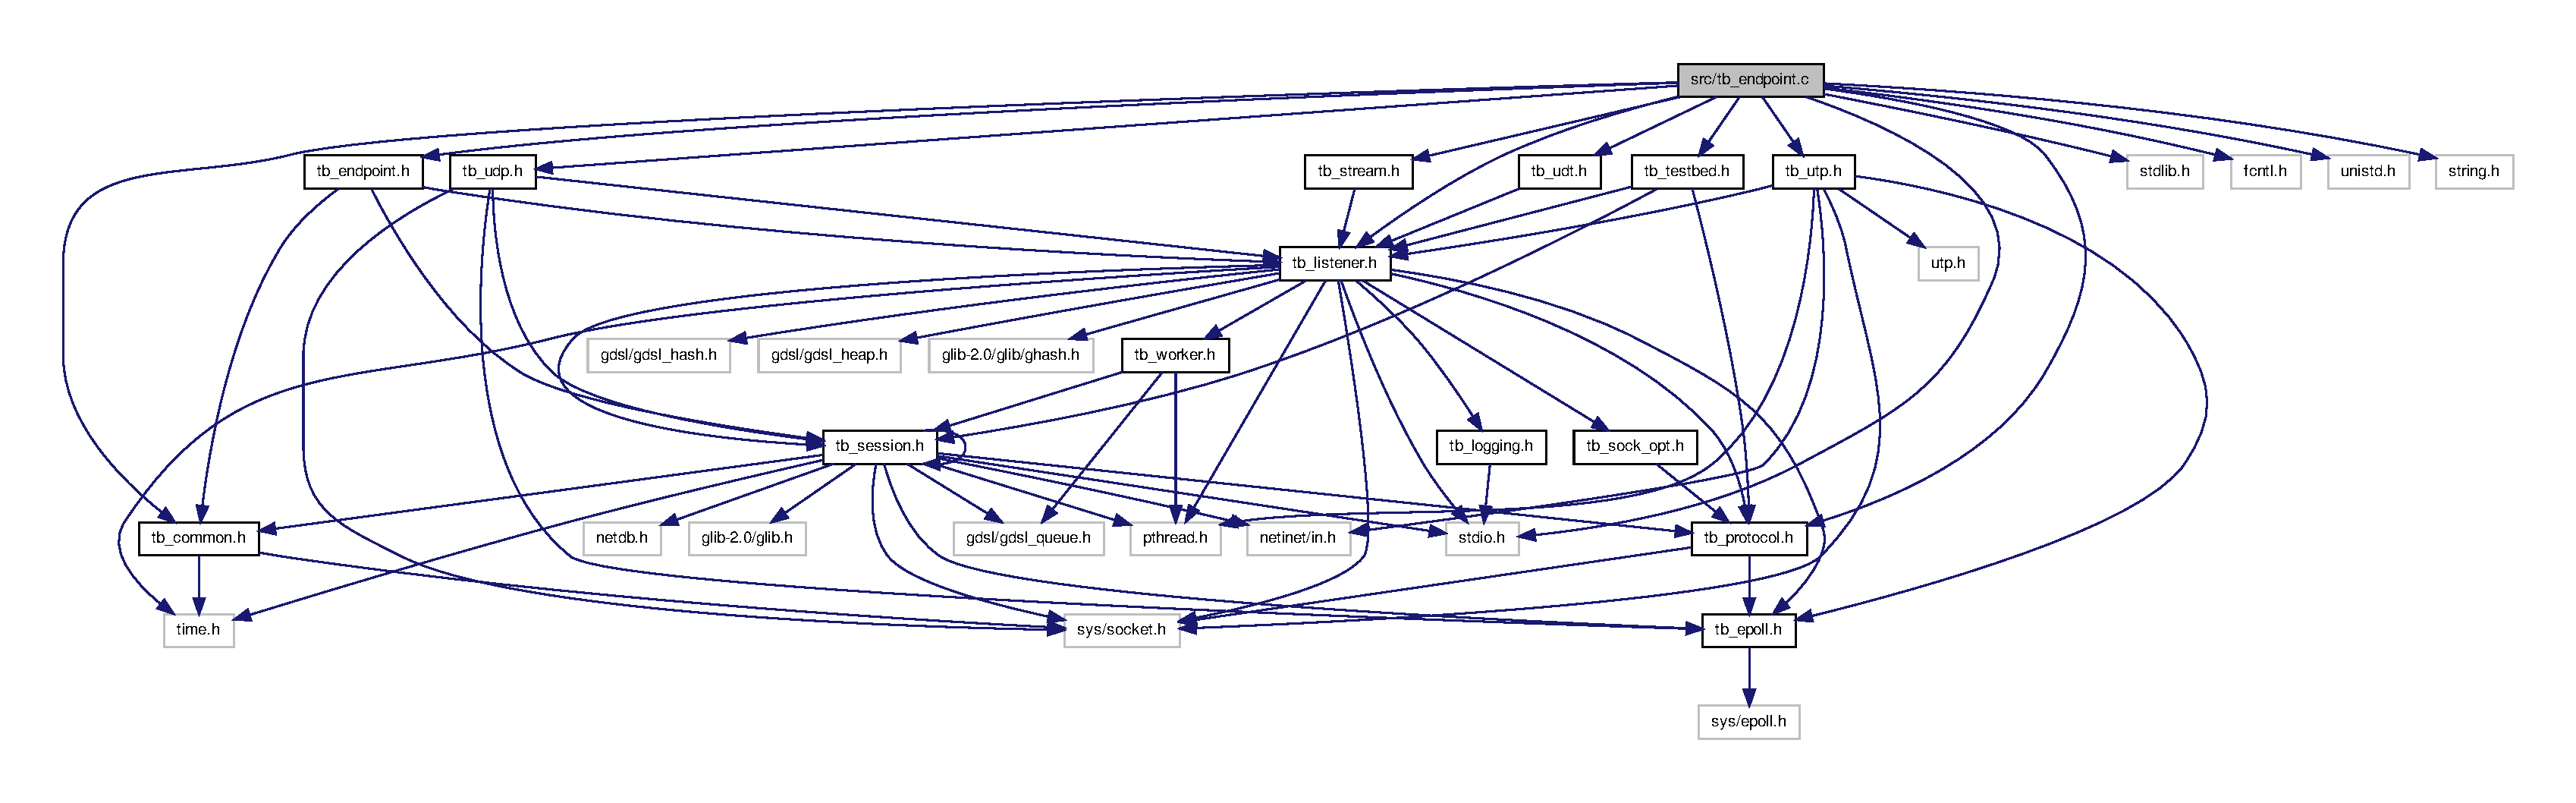
\includegraphics[width=350pt]{tb__endpoint_8c__incl}
\end{center}
\end{figure}
\subsection*{Functions}
\begin{DoxyCompactItemize}
\item 
void $\ast$ \hyperlink{tb__endpoint_8c_aef656bc85ab4f5554d4bf274c43c1ce7}{tb\-\_\-client} (void $\ast$data)
\begin{DoxyCompactList}\small\item\em Runs the client. \end{DoxyCompactList}\item 
void $\ast$ \hyperlink{tb__endpoint_8c_ad7d989dc2facd18964b22326b48b7d71}{tb\-\_\-server} (void $\ast$data)
\begin{DoxyCompactList}\small\item\em Runs the server. \end{DoxyCompactList}\end{DoxyCompactItemize}


\subsection{Function Documentation}
\hypertarget{tb__endpoint_8c_aef656bc85ab4f5554d4bf274c43c1ce7}{\index{tb\-\_\-endpoint.\-c@{tb\-\_\-endpoint.\-c}!tb\-\_\-client@{tb\-\_\-client}}
\index{tb\-\_\-client@{tb\-\_\-client}!tb_endpoint.c@{tb\-\_\-endpoint.\-c}}
\subsubsection[{tb\-\_\-client}]{\setlength{\rightskip}{0pt plus 5cm}void$\ast$ tb\-\_\-client (
\begin{DoxyParamCaption}
\item[{void $\ast$}]{data}
\end{DoxyParamCaption}
)}}\label{tb__endpoint_8c_aef656bc85ab4f5554d4bf274c43c1ce7}


Runs the client. 

Runs the client, called from pthread\-\_\-create.

\begin{DoxyPrecond}{Precondition}
data must be of type \hyperlink{structtb__listener__t}{tb\-\_\-listener\-\_\-t}. 
\end{DoxyPrecond}

\begin{DoxyParams}{Parameters}
{\em data} & Instance of \hyperlink{structtb__listener__t}{tb\-\_\-listener\-\_\-t} to run as client. \\
\hline
\end{DoxyParams}
\begin{DoxyReturn}{Returns}
As pthread\-\_\-exit is called, this does not return. 
\end{DoxyReturn}


Definition at line 30 of file tb\-\_\-endpoint.\-c.

\hypertarget{tb__endpoint_8c_ad7d989dc2facd18964b22326b48b7d71}{\index{tb\-\_\-endpoint.\-c@{tb\-\_\-endpoint.\-c}!tb\-\_\-server@{tb\-\_\-server}}
\index{tb\-\_\-server@{tb\-\_\-server}!tb_endpoint.c@{tb\-\_\-endpoint.\-c}}
\subsubsection[{tb\-\_\-server}]{\setlength{\rightskip}{0pt plus 5cm}void$\ast$ tb\-\_\-server (
\begin{DoxyParamCaption}
\item[{void $\ast$}]{data}
\end{DoxyParamCaption}
)}}\label{tb__endpoint_8c_ad7d989dc2facd18964b22326b48b7d71}


Runs the server. 

This starts a server instance, called from pthread\-\_\-create.

\begin{DoxyPrecond}{Precondition}
data must be of type \hyperlink{structtb__listener__t}{tb\-\_\-listener\-\_\-t}. 
\end{DoxyPrecond}

\begin{DoxyParams}{Parameters}
{\em data} & This is an instance of \hyperlink{structtb__listener__t}{tb\-\_\-listener\-\_\-t}. \\
\hline
\end{DoxyParams}
\begin{DoxyReturn}{Returns}
As pthread\-\_\-exit is called, this does not return. 
\end{DoxyReturn}


Definition at line 123 of file tb\-\_\-endpoint.\-c.


\hypertarget{tb__endpoint_8h}{\section{src/tb\-\_\-endpoint.h File Reference}
\label{tb__endpoint_8h}\index{src/tb\-\_\-endpoint.\-h@{src/tb\-\_\-endpoint.\-h}}
}
{\ttfamily \#include \char`\"{}tb\-\_\-listener.\-h\char`\"{}}\\*
{\ttfamily \#include \char`\"{}tb\-\_\-session.\-h\char`\"{}}\\*
{\ttfamily \#include \char`\"{}tb\-\_\-common.\-h\char`\"{}}\\*
Include dependency graph for tb\-\_\-endpoint.\-h\-:\nopagebreak
\begin{figure}[H]
\begin{center}
\leavevmode
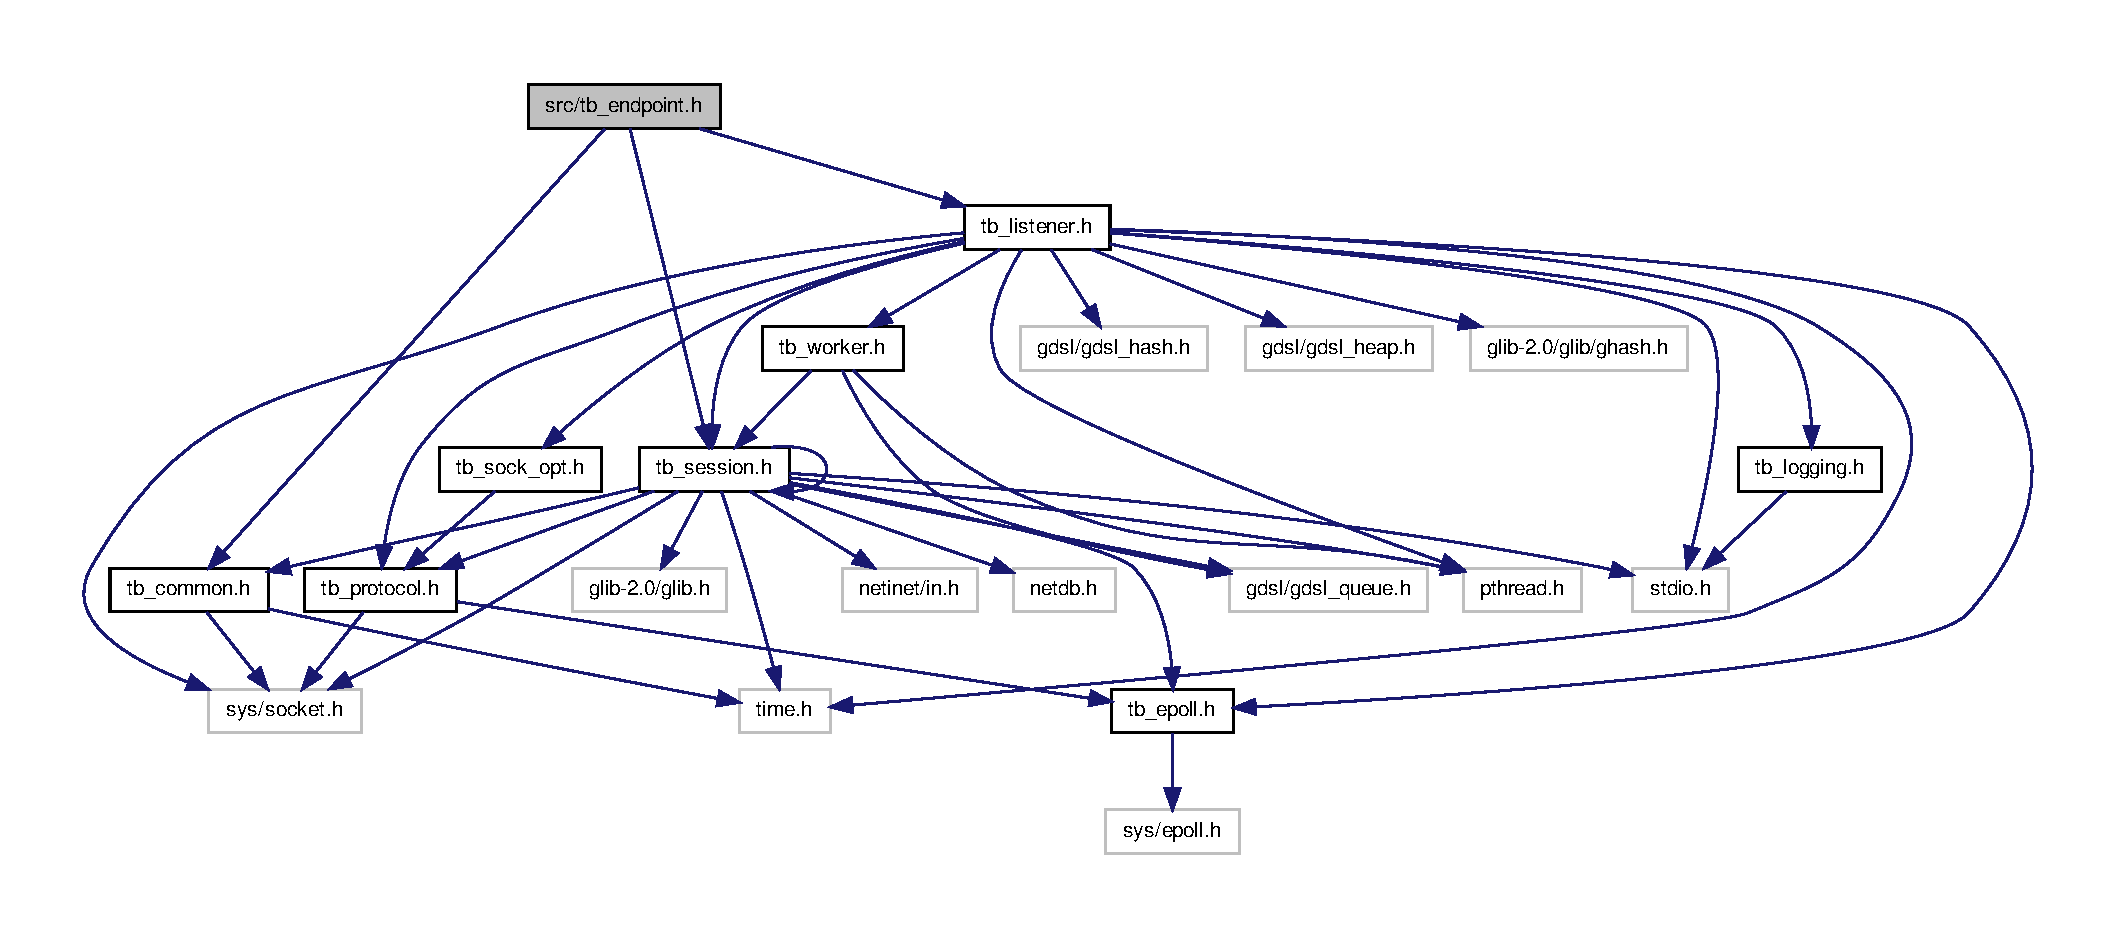
\includegraphics[width=350pt]{tb__endpoint_8h__incl}
\end{center}
\end{figure}
This graph shows which files directly or indirectly include this file\-:\nopagebreak
\begin{figure}[H]
\begin{center}
\leavevmode
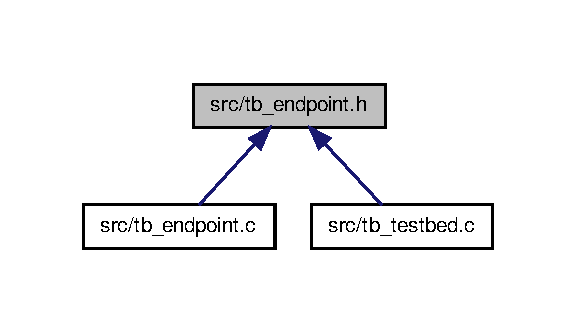
\includegraphics[width=276pt]{tb__endpoint_8h__dep__incl}
\end{center}
\end{figure}
\subsection*{Functions}
\begin{DoxyCompactItemize}
\item 
void $\ast$ \hyperlink{tb__endpoint_8h_ae38c1a880329aa4e19c7d646cebf6f23}{tb\-\_\-client} (void $\ast$data) \-\_\-\-\_\-attribute\-\_\-\-\_\-((\-\_\-\-\_\-noreturn\-\_\-\-\_\-))
\begin{DoxyCompactList}\small\item\em Runs the client. \end{DoxyCompactList}\item 
void $\ast$ \hyperlink{tb__endpoint_8h_afa271df665c1d414719366b433b88433}{tb\-\_\-server} (void $\ast$data) \-\_\-\-\_\-attribute\-\_\-\-\_\-((\-\_\-\-\_\-noreturn\-\_\-\-\_\-))
\begin{DoxyCompactList}\small\item\em Runs the server. \end{DoxyCompactList}\end{DoxyCompactItemize}


\subsection{Function Documentation}
\hypertarget{tb__endpoint_8h_ae38c1a880329aa4e19c7d646cebf6f23}{\index{tb\-\_\-endpoint.\-h@{tb\-\_\-endpoint.\-h}!tb\-\_\-client@{tb\-\_\-client}}
\index{tb\-\_\-client@{tb\-\_\-client}!tb_endpoint.h@{tb\-\_\-endpoint.\-h}}
\subsubsection[{tb\-\_\-client}]{\setlength{\rightskip}{0pt plus 5cm}void$\ast$ tb\-\_\-client (
\begin{DoxyParamCaption}
\item[{void $\ast$}]{data}
\end{DoxyParamCaption}
)}}\label{tb__endpoint_8h_ae38c1a880329aa4e19c7d646cebf6f23}


Runs the client. 

Runs the client, called from pthread\-\_\-create.

\begin{DoxyPrecond}{Precondition}
data must be of type \hyperlink{structtb__listener__t}{tb\-\_\-listener\-\_\-t}. 
\end{DoxyPrecond}

\begin{DoxyParams}{Parameters}
{\em data} & Instance of \hyperlink{structtb__listener__t}{tb\-\_\-listener\-\_\-t} to run as client. \\
\hline
\end{DoxyParams}
\begin{DoxyReturn}{Returns}
As pthread\-\_\-exit is called, this does not return. 
\end{DoxyReturn}


Definition at line 30 of file tb\-\_\-endpoint.\-c.

\hypertarget{tb__endpoint_8h_afa271df665c1d414719366b433b88433}{\index{tb\-\_\-endpoint.\-h@{tb\-\_\-endpoint.\-h}!tb\-\_\-server@{tb\-\_\-server}}
\index{tb\-\_\-server@{tb\-\_\-server}!tb_endpoint.h@{tb\-\_\-endpoint.\-h}}
\subsubsection[{tb\-\_\-server}]{\setlength{\rightskip}{0pt plus 5cm}void$\ast$ tb\-\_\-server (
\begin{DoxyParamCaption}
\item[{void $\ast$}]{data}
\end{DoxyParamCaption}
)}}\label{tb__endpoint_8h_afa271df665c1d414719366b433b88433}


Runs the server. 

This starts a server instance, called from pthread\-\_\-create.

\begin{DoxyPrecond}{Precondition}
data must be of type \hyperlink{structtb__listener__t}{tb\-\_\-listener\-\_\-t}. 
\end{DoxyPrecond}

\begin{DoxyParams}{Parameters}
{\em data} & This is an instance of \hyperlink{structtb__listener__t}{tb\-\_\-listener\-\_\-t}. \\
\hline
\end{DoxyParams}
\begin{DoxyReturn}{Returns}
As pthread\-\_\-exit is called, this does not return. 
\end{DoxyReturn}


Definition at line 114 of file tb\-\_\-endpoint.\-c.


\hypertarget{tb__epoll_8c}{\section{src/tb\-\_\-epoll.c File Reference}
\label{tb__epoll_8c}\index{src/tb\-\_\-epoll.\-c@{src/tb\-\_\-epoll.\-c}}
}
{\ttfamily \#include \char`\"{}tb\-\_\-epoll.\-h\char`\"{}}\\*
{\ttfamily \#include \char`\"{}tb\-\_\-common.\-h\char`\"{}}\\*
{\ttfamily \#include $<$sys/epoll.\-h$>$}\\*
{\ttfamily \#include $<$sys/fcntl.\-h$>$}\\*
{\ttfamily \#include $<$stdio.\-h$>$}\\*
{\ttfamily \#include $<$unistd.\-h$>$}\\*
{\ttfamily \#include $<$string.\-h$>$}\\*
Include dependency graph for tb\-\_\-epoll.\-c\-:\nopagebreak
\begin{figure}[H]
\begin{center}
\leavevmode
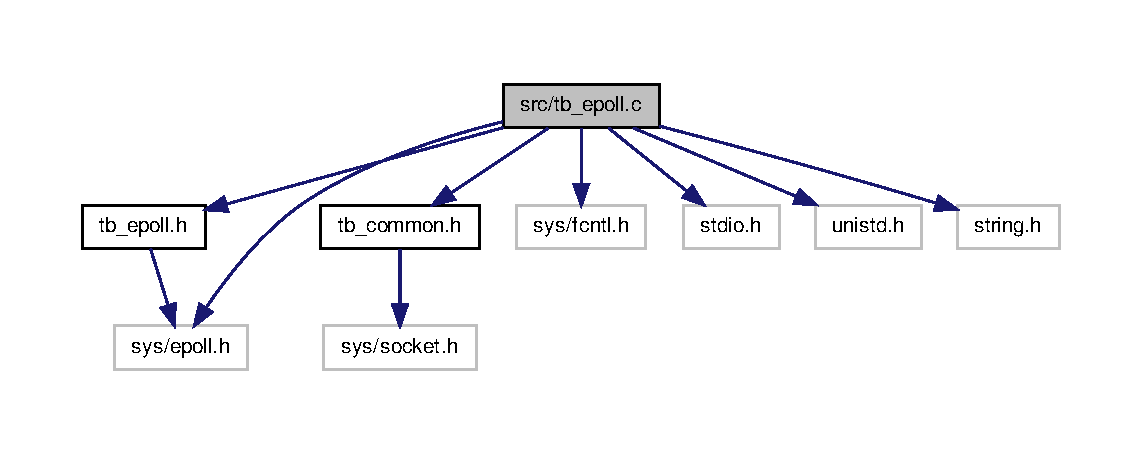
\includegraphics[width=350pt]{tb__epoll_8c__incl}
\end{center}
\end{figure}
\subsection*{Functions}
\begin{DoxyCompactItemize}
\item 
\hyperlink{structtb__epoll__t}{tb\-\_\-epoll\-\_\-t} $\ast$ \hyperlink{tb__epoll_8c_a7bcb4413b144b3a557b8f4ec916c95b4}{tb\-\_\-create\-\_\-e\-\_\-poll} (int sock\-\_\-d, int max\-\_\-events, int grp\-\_\-events, void $\ast$data)
\item 
void \hyperlink{tb__epoll_8c_aca14fd4146b5d1e3d4e111f0c381266c}{tb\-\_\-destroy\-\_\-epoll} (\hyperlink{structtb__epoll__t}{tb\-\_\-epoll\-\_\-t} $\ast$e\-\_\-poll)
\item 
int \hyperlink{tb__epoll_8c_a3edd81f86ea3c60986e557ebb68a4191}{tb\-\_\-add\-\_\-socket} (\hyperlink{structtb__epoll__t}{tb\-\_\-epoll\-\_\-t} $\ast$e\-\_\-poll, int sock\-\_\-d)
\item 
int \hyperlink{tb__epoll_8c_a13d79114c03d139cc28fc4643bec2073}{tb\-\_\-poll\-\_\-for\-\_\-events} (\hyperlink{structtb__epoll__t}{tb\-\_\-epoll\-\_\-t} $\ast$e\-\_\-poll)
\end{DoxyCompactItemize}
\subsection*{Variables}
\begin{DoxyCompactItemize}
\item 
const int \hyperlink{tb__epoll_8c_aa8f566169b1afefe7c0640ed0dc5d877}{event\-\_\-defaults} = E\-P\-O\-L\-L\-I\-N $|$ E\-P\-O\-L\-L\-E\-T
\end{DoxyCompactItemize}


\subsection{Function Documentation}
\hypertarget{tb__epoll_8c_a3edd81f86ea3c60986e557ebb68a4191}{\index{tb\-\_\-epoll.\-c@{tb\-\_\-epoll.\-c}!tb\-\_\-add\-\_\-socket@{tb\-\_\-add\-\_\-socket}}
\index{tb\-\_\-add\-\_\-socket@{tb\-\_\-add\-\_\-socket}!tb_epoll.c@{tb\-\_\-epoll.\-c}}
\subsubsection[{tb\-\_\-add\-\_\-socket}]{\setlength{\rightskip}{0pt plus 5cm}int tb\-\_\-add\-\_\-socket (
\begin{DoxyParamCaption}
\item[{{\bf tb\-\_\-epoll\-\_\-t} $\ast$}]{e\-\_\-poll, }
\item[{int}]{sock\-\_\-d}
\end{DoxyParamCaption}
)}}\label{tb__epoll_8c_a3edd81f86ea3c60986e557ebb68a4191}


Definition at line 76 of file tb\-\_\-epoll.\-c.

\hypertarget{tb__epoll_8c_a7bcb4413b144b3a557b8f4ec916c95b4}{\index{tb\-\_\-epoll.\-c@{tb\-\_\-epoll.\-c}!tb\-\_\-create\-\_\-e\-\_\-poll@{tb\-\_\-create\-\_\-e\-\_\-poll}}
\index{tb\-\_\-create\-\_\-e\-\_\-poll@{tb\-\_\-create\-\_\-e\-\_\-poll}!tb_epoll.c@{tb\-\_\-epoll.\-c}}
\subsubsection[{tb\-\_\-create\-\_\-e\-\_\-poll}]{\setlength{\rightskip}{0pt plus 5cm}{\bf tb\-\_\-epoll\-\_\-t}$\ast$ tb\-\_\-create\-\_\-e\-\_\-poll (
\begin{DoxyParamCaption}
\item[{int}]{sock\-\_\-d, }
\item[{int}]{max\-\_\-events, }
\item[{int}]{grp\-\_\-events, }
\item[{void $\ast$}]{data}
\end{DoxyParamCaption}
)}}\label{tb__epoll_8c_a7bcb4413b144b3a557b8f4ec916c95b4}


Definition at line 19 of file tb\-\_\-epoll.\-c.

\hypertarget{tb__epoll_8c_aca14fd4146b5d1e3d4e111f0c381266c}{\index{tb\-\_\-epoll.\-c@{tb\-\_\-epoll.\-c}!tb\-\_\-destroy\-\_\-epoll@{tb\-\_\-destroy\-\_\-epoll}}
\index{tb\-\_\-destroy\-\_\-epoll@{tb\-\_\-destroy\-\_\-epoll}!tb_epoll.c@{tb\-\_\-epoll.\-c}}
\subsubsection[{tb\-\_\-destroy\-\_\-epoll}]{\setlength{\rightskip}{0pt plus 5cm}void tb\-\_\-destroy\-\_\-epoll (
\begin{DoxyParamCaption}
\item[{{\bf tb\-\_\-epoll\-\_\-t} $\ast$}]{e\-\_\-poll}
\end{DoxyParamCaption}
)}}\label{tb__epoll_8c_aca14fd4146b5d1e3d4e111f0c381266c}


Definition at line 68 of file tb\-\_\-epoll.\-c.

\hypertarget{tb__epoll_8c_a13d79114c03d139cc28fc4643bec2073}{\index{tb\-\_\-epoll.\-c@{tb\-\_\-epoll.\-c}!tb\-\_\-poll\-\_\-for\-\_\-events@{tb\-\_\-poll\-\_\-for\-\_\-events}}
\index{tb\-\_\-poll\-\_\-for\-\_\-events@{tb\-\_\-poll\-\_\-for\-\_\-events}!tb_epoll.c@{tb\-\_\-epoll.\-c}}
\subsubsection[{tb\-\_\-poll\-\_\-for\-\_\-events}]{\setlength{\rightskip}{0pt plus 5cm}int tb\-\_\-poll\-\_\-for\-\_\-events (
\begin{DoxyParamCaption}
\item[{{\bf tb\-\_\-epoll\-\_\-t} $\ast$}]{e\-\_\-poll}
\end{DoxyParamCaption}
)}}\label{tb__epoll_8c_a13d79114c03d139cc28fc4643bec2073}


Definition at line 115 of file tb\-\_\-epoll.\-c.



\subsection{Variable Documentation}
\hypertarget{tb__epoll_8c_aa8f566169b1afefe7c0640ed0dc5d877}{\index{tb\-\_\-epoll.\-c@{tb\-\_\-epoll.\-c}!event\-\_\-defaults@{event\-\_\-defaults}}
\index{event\-\_\-defaults@{event\-\_\-defaults}!tb_epoll.c@{tb\-\_\-epoll.\-c}}
\subsubsection[{event\-\_\-defaults}]{\setlength{\rightskip}{0pt plus 5cm}const int event\-\_\-defaults = E\-P\-O\-L\-L\-I\-N $|$ E\-P\-O\-L\-L\-E\-T}}\label{tb__epoll_8c_aa8f566169b1afefe7c0640ed0dc5d877}


Definition at line 16 of file tb\-\_\-epoll.\-c.


\hypertarget{tb__epoll_8h}{\section{src/tb\-\_\-epoll.h File Reference}
\label{tb__epoll_8h}\index{src/tb\-\_\-epoll.\-h@{src/tb\-\_\-epoll.\-h}}
}
{\ttfamily \#include $<$sys/epoll.\-h$>$}\\*
Include dependency graph for tb\-\_\-epoll.\-h\-:\nopagebreak
\begin{figure}[H]
\begin{center}
\leavevmode
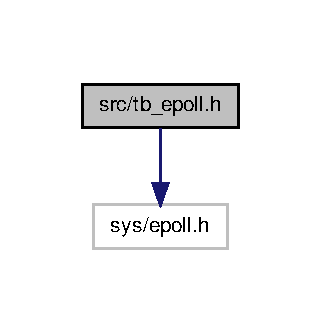
\includegraphics[width=154pt]{tb__epoll_8h__incl}
\end{center}
\end{figure}
This graph shows which files directly or indirectly include this file\-:\nopagebreak
\begin{figure}[H]
\begin{center}
\leavevmode
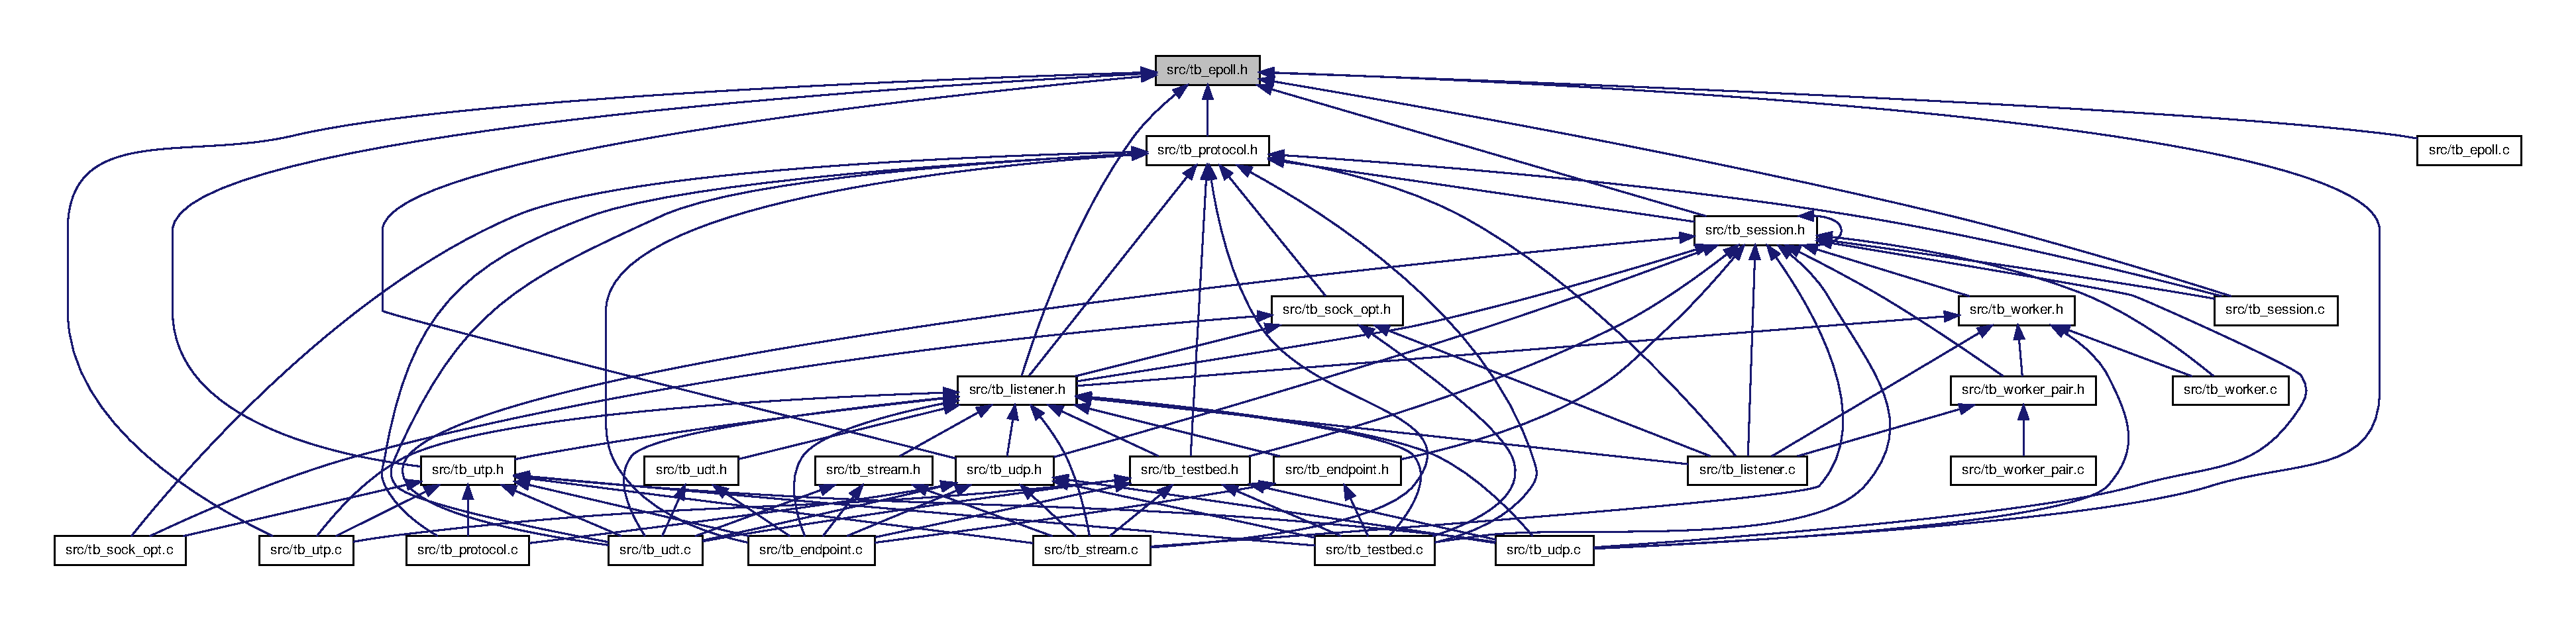
\includegraphics[width=350pt]{tb__epoll_8h__dep__incl}
\end{center}
\end{figure}
\subsection*{Data Structures}
\begin{DoxyCompactItemize}
\item 
struct \hyperlink{structtb__epoll__t}{tb\-\_\-epoll\-\_\-t}
\item 
struct \hyperlink{structtb__e__data}{tb\-\_\-e\-\_\-data}
\end{DoxyCompactItemize}
\subsection*{Typedefs}
\begin{DoxyCompactItemize}
\item 
typedef int($\ast$ \hyperlink{tb__epoll_8h_ab908abbc4a276702f09c05bdf565bd64}{func\-\_\-event} )(int events, void $\ast$data)
\begin{DoxyCompactList}\small\item\em Callback for events on the socket. \end{DoxyCompactList}\end{DoxyCompactItemize}
\subsection*{Functions}
\begin{DoxyCompactItemize}
\item 
\hyperlink{structtb__epoll__t}{tb\-\_\-epoll\-\_\-t} $\ast$ \hyperlink{tb__epoll_8h_a7bcb4413b144b3a557b8f4ec916c95b4}{tb\-\_\-create\-\_\-e\-\_\-poll} (int sock\-\_\-d, int max\-\_\-events, int grp\-\_\-events, void $\ast$data)
\item 
void \hyperlink{tb__epoll_8h_aca14fd4146b5d1e3d4e111f0c381266c}{tb\-\_\-destroy\-\_\-epoll} (\hyperlink{structtb__epoll__t}{tb\-\_\-epoll\-\_\-t} $\ast$e\-\_\-poll)
\item 
int \hyperlink{tb__epoll_8h_a3edd81f86ea3c60986e557ebb68a4191}{tb\-\_\-add\-\_\-socket} (\hyperlink{structtb__epoll__t}{tb\-\_\-epoll\-\_\-t} $\ast$e\-\_\-poll, int sock\-\_\-d)
\item 
int \hyperlink{tb__epoll_8h_a13d79114c03d139cc28fc4643bec2073}{tb\-\_\-poll\-\_\-for\-\_\-events} (\hyperlink{structtb__epoll__t}{tb\-\_\-epoll\-\_\-t} $\ast$e\-\_\-poll)
\end{DoxyCompactItemize}
\subsection*{Variables}
\begin{DoxyCompactItemize}
\item 
const int \hyperlink{tb__epoll_8h_aa8f566169b1afefe7c0640ed0dc5d877}{event\-\_\-defaults}
\end{DoxyCompactItemize}


\subsection{Typedef Documentation}
\hypertarget{tb__epoll_8h_ab908abbc4a276702f09c05bdf565bd64}{\index{tb\-\_\-epoll.\-h@{tb\-\_\-epoll.\-h}!func\-\_\-event@{func\-\_\-event}}
\index{func\-\_\-event@{func\-\_\-event}!tb_epoll.h@{tb\-\_\-epoll.\-h}}
\subsubsection[{func\-\_\-event}]{\setlength{\rightskip}{0pt plus 5cm}typedef int($\ast$ func\-\_\-event)(int events, void $\ast$data)}}\label{tb__epoll_8h_ab908abbc4a276702f09c05bdf565bd64}


Callback for events on the socket. 

This function is called when an event occurs for the given fd. 

Definition at line 20 of file tb\-\_\-epoll.\-h.



\subsection{Function Documentation}
\hypertarget{tb__epoll_8h_a3edd81f86ea3c60986e557ebb68a4191}{\index{tb\-\_\-epoll.\-h@{tb\-\_\-epoll.\-h}!tb\-\_\-add\-\_\-socket@{tb\-\_\-add\-\_\-socket}}
\index{tb\-\_\-add\-\_\-socket@{tb\-\_\-add\-\_\-socket}!tb_epoll.h@{tb\-\_\-epoll.\-h}}
\subsubsection[{tb\-\_\-add\-\_\-socket}]{\setlength{\rightskip}{0pt plus 5cm}int tb\-\_\-add\-\_\-socket (
\begin{DoxyParamCaption}
\item[{{\bf tb\-\_\-epoll\-\_\-t} $\ast$}]{e\-\_\-poll, }
\item[{int}]{sock\-\_\-d}
\end{DoxyParamCaption}
)}}\label{tb__epoll_8h_a3edd81f86ea3c60986e557ebb68a4191}


Definition at line 76 of file tb\-\_\-epoll.\-c.

\hypertarget{tb__epoll_8h_a7bcb4413b144b3a557b8f4ec916c95b4}{\index{tb\-\_\-epoll.\-h@{tb\-\_\-epoll.\-h}!tb\-\_\-create\-\_\-e\-\_\-poll@{tb\-\_\-create\-\_\-e\-\_\-poll}}
\index{tb\-\_\-create\-\_\-e\-\_\-poll@{tb\-\_\-create\-\_\-e\-\_\-poll}!tb_epoll.h@{tb\-\_\-epoll.\-h}}
\subsubsection[{tb\-\_\-create\-\_\-e\-\_\-poll}]{\setlength{\rightskip}{0pt plus 5cm}{\bf tb\-\_\-epoll\-\_\-t}$\ast$ tb\-\_\-create\-\_\-e\-\_\-poll (
\begin{DoxyParamCaption}
\item[{int}]{sock\-\_\-d, }
\item[{int}]{max\-\_\-events, }
\item[{int}]{grp\-\_\-events, }
\item[{void $\ast$}]{data}
\end{DoxyParamCaption}
)}}\label{tb__epoll_8h_a7bcb4413b144b3a557b8f4ec916c95b4}


Definition at line 19 of file tb\-\_\-epoll.\-c.

\hypertarget{tb__epoll_8h_aca14fd4146b5d1e3d4e111f0c381266c}{\index{tb\-\_\-epoll.\-h@{tb\-\_\-epoll.\-h}!tb\-\_\-destroy\-\_\-epoll@{tb\-\_\-destroy\-\_\-epoll}}
\index{tb\-\_\-destroy\-\_\-epoll@{tb\-\_\-destroy\-\_\-epoll}!tb_epoll.h@{tb\-\_\-epoll.\-h}}
\subsubsection[{tb\-\_\-destroy\-\_\-epoll}]{\setlength{\rightskip}{0pt plus 5cm}void tb\-\_\-destroy\-\_\-epoll (
\begin{DoxyParamCaption}
\item[{{\bf tb\-\_\-epoll\-\_\-t} $\ast$}]{e\-\_\-poll}
\end{DoxyParamCaption}
)}}\label{tb__epoll_8h_aca14fd4146b5d1e3d4e111f0c381266c}


Definition at line 68 of file tb\-\_\-epoll.\-c.

\hypertarget{tb__epoll_8h_a13d79114c03d139cc28fc4643bec2073}{\index{tb\-\_\-epoll.\-h@{tb\-\_\-epoll.\-h}!tb\-\_\-poll\-\_\-for\-\_\-events@{tb\-\_\-poll\-\_\-for\-\_\-events}}
\index{tb\-\_\-poll\-\_\-for\-\_\-events@{tb\-\_\-poll\-\_\-for\-\_\-events}!tb_epoll.h@{tb\-\_\-epoll.\-h}}
\subsubsection[{tb\-\_\-poll\-\_\-for\-\_\-events}]{\setlength{\rightskip}{0pt plus 5cm}int tb\-\_\-poll\-\_\-for\-\_\-events (
\begin{DoxyParamCaption}
\item[{{\bf tb\-\_\-epoll\-\_\-t} $\ast$}]{e\-\_\-poll}
\end{DoxyParamCaption}
)}}\label{tb__epoll_8h_a13d79114c03d139cc28fc4643bec2073}


Definition at line 115 of file tb\-\_\-epoll.\-c.



\subsection{Variable Documentation}
\hypertarget{tb__epoll_8h_aa8f566169b1afefe7c0640ed0dc5d877}{\index{tb\-\_\-epoll.\-h@{tb\-\_\-epoll.\-h}!event\-\_\-defaults@{event\-\_\-defaults}}
\index{event\-\_\-defaults@{event\-\_\-defaults}!tb_epoll.h@{tb\-\_\-epoll.\-h}}
\subsubsection[{event\-\_\-defaults}]{\setlength{\rightskip}{0pt plus 5cm}const int event\-\_\-defaults}}\label{tb__epoll_8h_aa8f566169b1afefe7c0640ed0dc5d877}


Definition at line 41 of file tb\-\_\-epoll.\-h.


\hypertarget{tb__file__io_8c}{\section{src/tb\-\_\-file\-\_\-io.c File Reference}
\label{tb__file__io_8c}\index{src/tb\-\_\-file\-\_\-io.\-c@{src/tb\-\_\-file\-\_\-io.\-c}}
}
{\ttfamily \#include \char`\"{}tb\-\_\-file\-\_\-io.\-h\char`\"{}}\\*
{\ttfamily \#include \char`\"{}tb\-\_\-common.\-h\char`\"{}}\\*
{\ttfamily \#include $<$string.\-h$>$}\\*
{\ttfamily \#include $<$unistd.\-h$>$}\\*
{\ttfamily \#include $<$fcntl.\-h$>$}\\*
{\ttfamily \#include $<$sys/stat.\-h$>$}\\*
{\ttfamily \#include $<$sys/mman.\-h$>$}\\*
{\ttfamily \#include $<$stdlib.\-h$>$}\\*
{\ttfamily \#include $<$libaio.\-h$>$}\\*
Include dependency graph for tb\-\_\-file\-\_\-io.\-c\-:\nopagebreak
\begin{figure}[H]
\begin{center}
\leavevmode
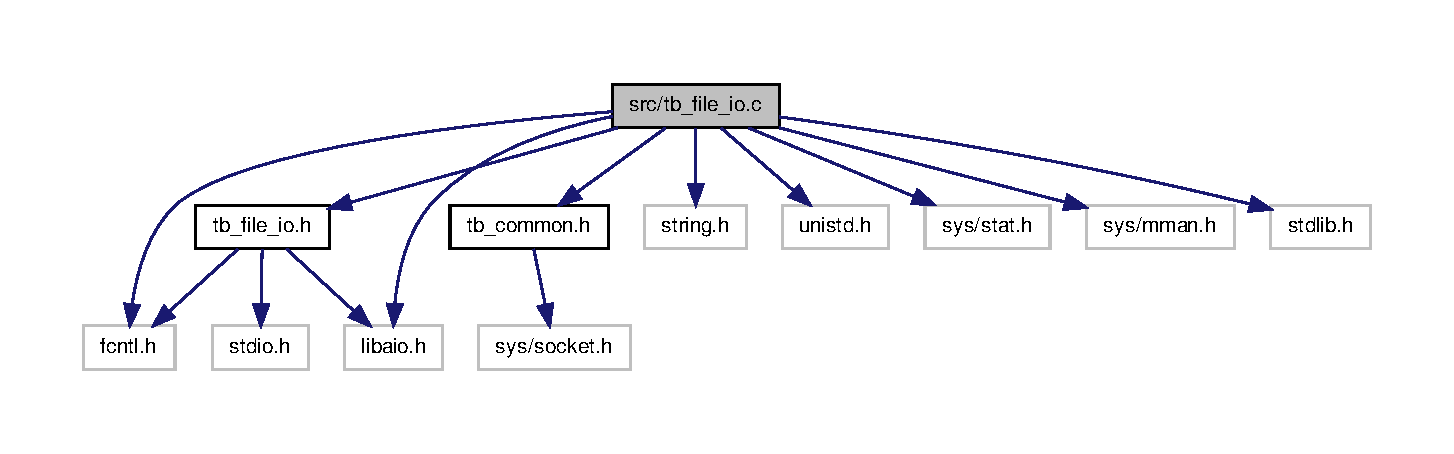
\includegraphics[width=350pt]{tb__file__io_8c__incl}
\end{center}
\end{figure}
\subsection*{Functions}
\begin{DoxyCompactItemize}
\item 
\hyperlink{structtb__file__t}{tb\-\_\-file\-\_\-t} $\ast$ \hyperlink{tb__file__io_8c_a34e8cc7a2fb9a9807fe122d73d833e69}{tb\-\_\-create\-\_\-file} (char $\ast$file\-\_\-path, \hyperlink{tb__file__io_8h_a365107762359ca7508e1b789f8f12c2b}{tb\-\_\-io\-\_\-type} type)
\begin{DoxyCompactList}\small\item\em Create \hyperlink{structtb__file__t}{tb\-\_\-file\-\_\-t}. \end{DoxyCompactList}\item 
int \hyperlink{tb__file__io_8c_abe2d48200f902cbf3ba8fac68c138ade}{tb\-\_\-destroy\-\_\-file} (\hyperlink{structtb__file__t}{tb\-\_\-file\-\_\-t} $\ast$file)
\begin{DoxyCompactList}\small\item\em Destroy \hyperlink{structtb__file__t}{tb\-\_\-file\-\_\-t}. \end{DoxyCompactList}\item 
void \hyperlink{tb__file__io_8c_a58c7b35b56dbdba2ee4f7b8a506221d2}{tb\-\_\-close\-\_\-destroy} (\hyperlink{structtb__file__t}{tb\-\_\-file\-\_\-t} $\ast$file)
\item 
int \hyperlink{tb__file__io_8c_a3fc47ba41d9efb07579f2325fb34f048}{tb\-\_\-get\-\_\-file\-\_\-length} (int fd)
\item 
\hyperlink{structtb__file__t}{tb\-\_\-file\-\_\-t} $\ast$ \hyperlink{tb__file__io_8c_a8923d7ac413049b32a80b7d5bb4862bc}{tb\-\_\-setup\-\_\-mmap} (char $\ast$file\-\_\-path, \hyperlink{tb__file__io_8h_a6393ed40c2daaa55fe6411ff7b4a4e61}{tb\-\_\-o\-\_\-flags} flags, int file\-\_\-len)
\begin{DoxyCompactList}\small\item\em Setup mmap for io. \end{DoxyCompactList}\item 
int \hyperlink{tb__file__io_8c_ac261d5433c8e8ebb01207507d721b6af}{tb\-\_\-write\-\_\-mmap} (\hyperlink{structtb__file__t}{tb\-\_\-file\-\_\-t} $\ast$file, char $\ast$buff, int off, int len)
\begin{DoxyCompactList}\small\item\em Write to a file using mmap. \end{DoxyCompactList}\item 
int \hyperlink{tb__file__io_8c_a95c8bd486da1d188d5f0636a492d06fe}{tb\-\_\-read\-\_\-mmap} (\hyperlink{structtb__file__t}{tb\-\_\-file\-\_\-t} $\ast$file, char $\ast$buff, int off, int len)
\begin{DoxyCompactList}\small\item\em Read a file using mmap. \end{DoxyCompactList}\item 
int \hyperlink{tb__file__io_8c_a55a2fd2fc6edd2180d781b6a34582df9}{tb\-\_\-close\-\_\-mmap} (\hyperlink{structtb__file__t}{tb\-\_\-file\-\_\-t} $\ast$file)
\begin{DoxyCompactList}\small\item\em close mmap. \end{DoxyCompactList}\item 
\hyperlink{structtb__file__t}{tb\-\_\-file\-\_\-t} $\ast$ \hyperlink{tb__file__io_8c_a9f5f4287c8757462a0c0ad86864049a1}{tb\-\_\-setup\-\_\-s} (char $\ast$file\-\_\-path, \hyperlink{tb__file__io_8h_a6393ed40c2daaa55fe6411ff7b4a4e61}{tb\-\_\-o\-\_\-flags} flags, int file\-\_\-len)
\begin{DoxyCompactList}\small\item\em Setup for synchronous io. \end{DoxyCompactList}\item 
int \hyperlink{tb__file__io_8c_a667112cc7e28387f256291eab00ace57}{tb\-\_\-close\-\_\-s} (\hyperlink{structtb__file__t}{tb\-\_\-file\-\_\-t} $\ast$file)
\begin{DoxyCompactList}\small\item\em Close for synchronous io. \end{DoxyCompactList}\item 
int \hyperlink{tb__file__io_8c_a49f736bb63ef24cca0dc00838fee96f4}{tb\-\_\-read\-\_\-s} (\hyperlink{structtb__file__t}{tb\-\_\-file\-\_\-t} $\ast$file, char $\ast$buf, int off, int len)
\begin{DoxyCompactList}\small\item\em Read a file synchronously. \end{DoxyCompactList}\item 
int \hyperlink{tb__file__io_8c_af7c9fa06df83c0f419e2b4aac6081298}{tb\-\_\-write\-\_\-s} (\hyperlink{structtb__file__t}{tb\-\_\-file\-\_\-t} $\ast$file, char $\ast$buf, int off, int len)
\begin{DoxyCompactList}\small\item\em Write to a file synchronously. \end{DoxyCompactList}\item 
\hyperlink{structtb__file__t}{tb\-\_\-file\-\_\-t} $\ast$ \hyperlink{tb__file__io_8c_a9d820528f4e06a8a1f3e9698fb42e8c1}{tb\-\_\-setup\-\_\-buffs} (char $\ast$file\-\_\-path, \hyperlink{tb__file__io_8h_a6393ed40c2daaa55fe6411ff7b4a4e61}{tb\-\_\-o\-\_\-flags} flags, int file\-\_\-len)
\item 
int \hyperlink{tb__file__io_8c_a7fddda8aa5dd31d0e828e1e19d895f64}{tb\-\_\-write\-\_\-buffs} (\hyperlink{structtb__file__t}{tb\-\_\-file\-\_\-t} $\ast$file, char $\ast$buf, int off, int len)
\item 
int \hyperlink{tb__file__io_8c_a6c960255bd187281dee5391fd8752e02}{tb\-\_\-read\-\_\-buffs} (\hyperlink{structtb__file__t}{tb\-\_\-file\-\_\-t} $\ast$file, char $\ast$buf, int off, int len)
\item 
int \hyperlink{tb__file__io_8c_a3958f06dac0c99ad9868ec8911024738}{tb\-\_\-close\-\_\-buffs} (\hyperlink{structtb__file__t}{tb\-\_\-file\-\_\-t} $\ast$file)
\item 
\hyperlink{structtb__file__t}{tb\-\_\-file\-\_\-t} $\ast$ \hyperlink{tb__file__io_8c_a30bcba636e8426f96642f70abd11bddd}{tb\-\_\-setup\-\_\-as} (char $\ast$file\-\_\-path)
\begin{DoxyCompactList}\small\item\em Setup asynchronous io. \end{DoxyCompactList}\item 
int \hyperlink{tb__file__io_8c_ac057b3b466672d56324d1f005e62c91b}{tb\-\_\-read\-\_\-as} (\hyperlink{structtb__file__t}{tb\-\_\-file\-\_\-t} $\ast$file)
\begin{DoxyCompactList}\small\item\em Read a file asynchronously. \end{DoxyCompactList}\item 
int \hyperlink{tb__file__io_8c_a45134b687c7902939c6a3d07ae9422a7}{tb\-\_\-write\-\_\-as} (\hyperlink{structtb__file__t}{tb\-\_\-file\-\_\-t} $\ast$file)
\begin{DoxyCompactList}\small\item\em Write to a file asynchronously. \end{DoxyCompactList}\item 
int \hyperlink{tb__file__io_8c_aa936b3880e816db9b609f4949c4c281c}{tb\-\_\-close\-\_\-as} (\hyperlink{structtb__file__t}{tb\-\_\-file\-\_\-t} $\ast$file)
\begin{DoxyCompactList}\small\item\em Close asynchronous io. \end{DoxyCompactList}\end{DoxyCompactItemize}


\subsection{Function Documentation}
\hypertarget{tb__file__io_8c_aa936b3880e816db9b609f4949c4c281c}{\index{tb\-\_\-file\-\_\-io.\-c@{tb\-\_\-file\-\_\-io.\-c}!tb\-\_\-close\-\_\-as@{tb\-\_\-close\-\_\-as}}
\index{tb\-\_\-close\-\_\-as@{tb\-\_\-close\-\_\-as}!tb_file_io.c@{tb\-\_\-file\-\_\-io.\-c}}
\subsubsection[{tb\-\_\-close\-\_\-as}]{\setlength{\rightskip}{0pt plus 5cm}int tb\-\_\-close\-\_\-as (
\begin{DoxyParamCaption}
\item[{{\bf tb\-\_\-file\-\_\-t} $\ast$}]{file}
\end{DoxyParamCaption}
)}}\label{tb__file__io_8c_aa936b3880e816db9b609f4949c4c281c}


Close asynchronous io. 



Definition at line 364 of file tb\-\_\-file\-\_\-io.\-c.

\hypertarget{tb__file__io_8c_a3958f06dac0c99ad9868ec8911024738}{\index{tb\-\_\-file\-\_\-io.\-c@{tb\-\_\-file\-\_\-io.\-c}!tb\-\_\-close\-\_\-buffs@{tb\-\_\-close\-\_\-buffs}}
\index{tb\-\_\-close\-\_\-buffs@{tb\-\_\-close\-\_\-buffs}!tb_file_io.c@{tb\-\_\-file\-\_\-io.\-c}}
\subsubsection[{tb\-\_\-close\-\_\-buffs}]{\setlength{\rightskip}{0pt plus 5cm}int tb\-\_\-close\-\_\-buffs (
\begin{DoxyParamCaption}
\item[{{\bf tb\-\_\-file\-\_\-t} $\ast$}]{file}
\end{DoxyParamCaption}
)}}\label{tb__file__io_8c_a3958f06dac0c99ad9868ec8911024738}


Definition at line 313 of file tb\-\_\-file\-\_\-io.\-c.

\hypertarget{tb__file__io_8c_a58c7b35b56dbdba2ee4f7b8a506221d2}{\index{tb\-\_\-file\-\_\-io.\-c@{tb\-\_\-file\-\_\-io.\-c}!tb\-\_\-close\-\_\-destroy@{tb\-\_\-close\-\_\-destroy}}
\index{tb\-\_\-close\-\_\-destroy@{tb\-\_\-close\-\_\-destroy}!tb_file_io.c@{tb\-\_\-file\-\_\-io.\-c}}
\subsubsection[{tb\-\_\-close\-\_\-destroy}]{\setlength{\rightskip}{0pt plus 5cm}void tb\-\_\-close\-\_\-destroy (
\begin{DoxyParamCaption}
\item[{{\bf tb\-\_\-file\-\_\-t} $\ast$}]{file}
\end{DoxyParamCaption}
)\hspace{0.3cm}{\ttfamily [inline]}}}\label{tb__file__io_8c_a58c7b35b56dbdba2ee4f7b8a506221d2}


Definition at line 37 of file tb\-\_\-file\-\_\-io.\-c.

\hypertarget{tb__file__io_8c_a55a2fd2fc6edd2180d781b6a34582df9}{\index{tb\-\_\-file\-\_\-io.\-c@{tb\-\_\-file\-\_\-io.\-c}!tb\-\_\-close\-\_\-mmap@{tb\-\_\-close\-\_\-mmap}}
\index{tb\-\_\-close\-\_\-mmap@{tb\-\_\-close\-\_\-mmap}!tb_file_io.c@{tb\-\_\-file\-\_\-io.\-c}}
\subsubsection[{tb\-\_\-close\-\_\-mmap}]{\setlength{\rightskip}{0pt plus 5cm}int tb\-\_\-close\-\_\-mmap (
\begin{DoxyParamCaption}
\item[{{\bf tb\-\_\-file\-\_\-t} $\ast$}]{file}
\end{DoxyParamCaption}
)}}\label{tb__file__io_8c_a55a2fd2fc6edd2180d781b6a34582df9}


close mmap. 



Definition at line 139 of file tb\-\_\-file\-\_\-io.\-c.

\hypertarget{tb__file__io_8c_a667112cc7e28387f256291eab00ace57}{\index{tb\-\_\-file\-\_\-io.\-c@{tb\-\_\-file\-\_\-io.\-c}!tb\-\_\-close\-\_\-s@{tb\-\_\-close\-\_\-s}}
\index{tb\-\_\-close\-\_\-s@{tb\-\_\-close\-\_\-s}!tb_file_io.c@{tb\-\_\-file\-\_\-io.\-c}}
\subsubsection[{tb\-\_\-close\-\_\-s}]{\setlength{\rightskip}{0pt plus 5cm}int tb\-\_\-close\-\_\-s (
\begin{DoxyParamCaption}
\item[{{\bf tb\-\_\-file\-\_\-t} $\ast$}]{file}
\end{DoxyParamCaption}
)}}\label{tb__file__io_8c_a667112cc7e28387f256291eab00ace57}


Close for synchronous io. 



Definition at line 182 of file tb\-\_\-file\-\_\-io.\-c.

\hypertarget{tb__file__io_8c_a34e8cc7a2fb9a9807fe122d73d833e69}{\index{tb\-\_\-file\-\_\-io.\-c@{tb\-\_\-file\-\_\-io.\-c}!tb\-\_\-create\-\_\-file@{tb\-\_\-create\-\_\-file}}
\index{tb\-\_\-create\-\_\-file@{tb\-\_\-create\-\_\-file}!tb_file_io.c@{tb\-\_\-file\-\_\-io.\-c}}
\subsubsection[{tb\-\_\-create\-\_\-file}]{\setlength{\rightskip}{0pt plus 5cm}{\bf tb\-\_\-file\-\_\-t}$\ast$ tb\-\_\-create\-\_\-file (
\begin{DoxyParamCaption}
\item[{char $\ast$}]{file\-\_\-path, }
\item[{{\bf tb\-\_\-io\-\_\-type}}]{type}
\end{DoxyParamCaption}
)\hspace{0.3cm}{\ttfamily [inline]}}}\label{tb__file__io_8c_a34e8cc7a2fb9a9807fe122d73d833e69}


Create \hyperlink{structtb__file__t}{tb\-\_\-file\-\_\-t}. 


\begin{DoxyItemize}
\item 
\end{DoxyItemize}

Definition at line 20 of file tb\-\_\-file\-\_\-io.\-c.

\hypertarget{tb__file__io_8c_abe2d48200f902cbf3ba8fac68c138ade}{\index{tb\-\_\-file\-\_\-io.\-c@{tb\-\_\-file\-\_\-io.\-c}!tb\-\_\-destroy\-\_\-file@{tb\-\_\-destroy\-\_\-file}}
\index{tb\-\_\-destroy\-\_\-file@{tb\-\_\-destroy\-\_\-file}!tb_file_io.c@{tb\-\_\-file\-\_\-io.\-c}}
\subsubsection[{tb\-\_\-destroy\-\_\-file}]{\setlength{\rightskip}{0pt plus 5cm}int tb\-\_\-destroy\-\_\-file (
\begin{DoxyParamCaption}
\item[{{\bf tb\-\_\-file\-\_\-t} $\ast$}]{file}
\end{DoxyParamCaption}
)\hspace{0.3cm}{\ttfamily [inline]}}}\label{tb__file__io_8c_abe2d48200f902cbf3ba8fac68c138ade}


Destroy \hyperlink{structtb__file__t}{tb\-\_\-file\-\_\-t}. 



Definition at line 29 of file tb\-\_\-file\-\_\-io.\-c.

\hypertarget{tb__file__io_8c_a3fc47ba41d9efb07579f2325fb34f048}{\index{tb\-\_\-file\-\_\-io.\-c@{tb\-\_\-file\-\_\-io.\-c}!tb\-\_\-get\-\_\-file\-\_\-length@{tb\-\_\-get\-\_\-file\-\_\-length}}
\index{tb\-\_\-get\-\_\-file\-\_\-length@{tb\-\_\-get\-\_\-file\-\_\-length}!tb_file_io.c@{tb\-\_\-file\-\_\-io.\-c}}
\subsubsection[{tb\-\_\-get\-\_\-file\-\_\-length}]{\setlength{\rightskip}{0pt plus 5cm}int tb\-\_\-get\-\_\-file\-\_\-length (
\begin{DoxyParamCaption}
\item[{int}]{fd}
\end{DoxyParamCaption}
)\hspace{0.3cm}{\ttfamily [inline]}}}\label{tb__file__io_8c_a3fc47ba41d9efb07579f2325fb34f048}


Definition at line 44 of file tb\-\_\-file\-\_\-io.\-c.

\hypertarget{tb__file__io_8c_ac057b3b466672d56324d1f005e62c91b}{\index{tb\-\_\-file\-\_\-io.\-c@{tb\-\_\-file\-\_\-io.\-c}!tb\-\_\-read\-\_\-as@{tb\-\_\-read\-\_\-as}}
\index{tb\-\_\-read\-\_\-as@{tb\-\_\-read\-\_\-as}!tb_file_io.c@{tb\-\_\-file\-\_\-io.\-c}}
\subsubsection[{tb\-\_\-read\-\_\-as}]{\setlength{\rightskip}{0pt plus 5cm}int tb\-\_\-read\-\_\-as (
\begin{DoxyParamCaption}
\item[{{\bf tb\-\_\-file\-\_\-t} $\ast$}]{file}
\end{DoxyParamCaption}
)}}\label{tb__file__io_8c_ac057b3b466672d56324d1f005e62c91b}


Read a file asynchronously. 



Definition at line 346 of file tb\-\_\-file\-\_\-io.\-c.

\hypertarget{tb__file__io_8c_a6c960255bd187281dee5391fd8752e02}{\index{tb\-\_\-file\-\_\-io.\-c@{tb\-\_\-file\-\_\-io.\-c}!tb\-\_\-read\-\_\-buffs@{tb\-\_\-read\-\_\-buffs}}
\index{tb\-\_\-read\-\_\-buffs@{tb\-\_\-read\-\_\-buffs}!tb_file_io.c@{tb\-\_\-file\-\_\-io.\-c}}
\subsubsection[{tb\-\_\-read\-\_\-buffs}]{\setlength{\rightskip}{0pt plus 5cm}int tb\-\_\-read\-\_\-buffs (
\begin{DoxyParamCaption}
\item[{{\bf tb\-\_\-file\-\_\-t} $\ast$}]{file, }
\item[{char $\ast$}]{buf, }
\item[{int}]{off, }
\item[{int}]{len}
\end{DoxyParamCaption}
)}}\label{tb__file__io_8c_a6c960255bd187281dee5391fd8752e02}


Definition at line 299 of file tb\-\_\-file\-\_\-io.\-c.

\hypertarget{tb__file__io_8c_a95c8bd486da1d188d5f0636a492d06fe}{\index{tb\-\_\-file\-\_\-io.\-c@{tb\-\_\-file\-\_\-io.\-c}!tb\-\_\-read\-\_\-mmap@{tb\-\_\-read\-\_\-mmap}}
\index{tb\-\_\-read\-\_\-mmap@{tb\-\_\-read\-\_\-mmap}!tb_file_io.c@{tb\-\_\-file\-\_\-io.\-c}}
\subsubsection[{tb\-\_\-read\-\_\-mmap}]{\setlength{\rightskip}{0pt plus 5cm}int tb\-\_\-read\-\_\-mmap (
\begin{DoxyParamCaption}
\item[{{\bf tb\-\_\-file\-\_\-t} $\ast$}]{file, }
\item[{char $\ast$}]{buff, }
\item[{int}]{off, }
\item[{int}]{len}
\end{DoxyParamCaption}
)}}\label{tb__file__io_8c_a95c8bd486da1d188d5f0636a492d06fe}


Read a file using mmap. 



Definition at line 128 of file tb\-\_\-file\-\_\-io.\-c.

\hypertarget{tb__file__io_8c_a49f736bb63ef24cca0dc00838fee96f4}{\index{tb\-\_\-file\-\_\-io.\-c@{tb\-\_\-file\-\_\-io.\-c}!tb\-\_\-read\-\_\-s@{tb\-\_\-read\-\_\-s}}
\index{tb\-\_\-read\-\_\-s@{tb\-\_\-read\-\_\-s}!tb_file_io.c@{tb\-\_\-file\-\_\-io.\-c}}
\subsubsection[{tb\-\_\-read\-\_\-s}]{\setlength{\rightskip}{0pt plus 5cm}int tb\-\_\-read\-\_\-s (
\begin{DoxyParamCaption}
\item[{{\bf tb\-\_\-file\-\_\-t} $\ast$}]{file, }
\item[{char $\ast$}]{buf, }
\item[{int}]{off, }
\item[{int}]{len}
\end{DoxyParamCaption}
)}}\label{tb__file__io_8c_a49f736bb63ef24cca0dc00838fee96f4}


Read a file synchronously. 



Definition at line 193 of file tb\-\_\-file\-\_\-io.\-c.

\hypertarget{tb__file__io_8c_a30bcba636e8426f96642f70abd11bddd}{\index{tb\-\_\-file\-\_\-io.\-c@{tb\-\_\-file\-\_\-io.\-c}!tb\-\_\-setup\-\_\-as@{tb\-\_\-setup\-\_\-as}}
\index{tb\-\_\-setup\-\_\-as@{tb\-\_\-setup\-\_\-as}!tb_file_io.c@{tb\-\_\-file\-\_\-io.\-c}}
\subsubsection[{tb\-\_\-setup\-\_\-as}]{\setlength{\rightskip}{0pt plus 5cm}{\bf tb\-\_\-file\-\_\-t}$\ast$ tb\-\_\-setup\-\_\-as (
\begin{DoxyParamCaption}
\item[{char $\ast$}]{file\-\_\-path}
\end{DoxyParamCaption}
)}}\label{tb__file__io_8c_a30bcba636e8426f96642f70abd11bddd}


Setup asynchronous io. 



Definition at line 325 of file tb\-\_\-file\-\_\-io.\-c.

\hypertarget{tb__file__io_8c_a9d820528f4e06a8a1f3e9698fb42e8c1}{\index{tb\-\_\-file\-\_\-io.\-c@{tb\-\_\-file\-\_\-io.\-c}!tb\-\_\-setup\-\_\-buffs@{tb\-\_\-setup\-\_\-buffs}}
\index{tb\-\_\-setup\-\_\-buffs@{tb\-\_\-setup\-\_\-buffs}!tb_file_io.c@{tb\-\_\-file\-\_\-io.\-c}}
\subsubsection[{tb\-\_\-setup\-\_\-buffs}]{\setlength{\rightskip}{0pt plus 5cm}{\bf tb\-\_\-file\-\_\-t}$\ast$ tb\-\_\-setup\-\_\-buffs (
\begin{DoxyParamCaption}
\item[{char $\ast$}]{file\-\_\-path, }
\item[{{\bf tb\-\_\-o\-\_\-flags}}]{flags, }
\item[{int}]{file\-\_\-len}
\end{DoxyParamCaption}
)}}\label{tb__file__io_8c_a9d820528f4e06a8a1f3e9698fb42e8c1}


Definition at line 232 of file tb\-\_\-file\-\_\-io.\-c.

\hypertarget{tb__file__io_8c_a8923d7ac413049b32a80b7d5bb4862bc}{\index{tb\-\_\-file\-\_\-io.\-c@{tb\-\_\-file\-\_\-io.\-c}!tb\-\_\-setup\-\_\-mmap@{tb\-\_\-setup\-\_\-mmap}}
\index{tb\-\_\-setup\-\_\-mmap@{tb\-\_\-setup\-\_\-mmap}!tb_file_io.c@{tb\-\_\-file\-\_\-io.\-c}}
\subsubsection[{tb\-\_\-setup\-\_\-mmap}]{\setlength{\rightskip}{0pt plus 5cm}{\bf tb\-\_\-file\-\_\-t}$\ast$ tb\-\_\-setup\-\_\-mmap (
\begin{DoxyParamCaption}
\item[{char $\ast$}]{file\-\_\-path, }
\item[{{\bf tb\-\_\-o\-\_\-flags}}]{flags, }
\item[{int}]{file\-\_\-len}
\end{DoxyParamCaption}
)}}\label{tb__file__io_8c_a8923d7ac413049b32a80b7d5bb4862bc}


Setup mmap for io. 



Definition at line 66 of file tb\-\_\-file\-\_\-io.\-c.

\hypertarget{tb__file__io_8c_a9f5f4287c8757462a0c0ad86864049a1}{\index{tb\-\_\-file\-\_\-io.\-c@{tb\-\_\-file\-\_\-io.\-c}!tb\-\_\-setup\-\_\-s@{tb\-\_\-setup\-\_\-s}}
\index{tb\-\_\-setup\-\_\-s@{tb\-\_\-setup\-\_\-s}!tb_file_io.c@{tb\-\_\-file\-\_\-io.\-c}}
\subsubsection[{tb\-\_\-setup\-\_\-s}]{\setlength{\rightskip}{0pt plus 5cm}{\bf tb\-\_\-file\-\_\-t}$\ast$ tb\-\_\-setup\-\_\-s (
\begin{DoxyParamCaption}
\item[{char $\ast$}]{file\-\_\-path, }
\item[{{\bf tb\-\_\-o\-\_\-flags}}]{flags, }
\item[{int}]{file\-\_\-len}
\end{DoxyParamCaption}
)}}\label{tb__file__io_8c_a9f5f4287c8757462a0c0ad86864049a1}


Setup for synchronous io. 



Definition at line 151 of file tb\-\_\-file\-\_\-io.\-c.

\hypertarget{tb__file__io_8c_a45134b687c7902939c6a3d07ae9422a7}{\index{tb\-\_\-file\-\_\-io.\-c@{tb\-\_\-file\-\_\-io.\-c}!tb\-\_\-write\-\_\-as@{tb\-\_\-write\-\_\-as}}
\index{tb\-\_\-write\-\_\-as@{tb\-\_\-write\-\_\-as}!tb_file_io.c@{tb\-\_\-file\-\_\-io.\-c}}
\subsubsection[{tb\-\_\-write\-\_\-as}]{\setlength{\rightskip}{0pt plus 5cm}int tb\-\_\-write\-\_\-as (
\begin{DoxyParamCaption}
\item[{{\bf tb\-\_\-file\-\_\-t} $\ast$}]{file}
\end{DoxyParamCaption}
)}}\label{tb__file__io_8c_a45134b687c7902939c6a3d07ae9422a7}


Write to a file asynchronously. 



Definition at line 355 of file tb\-\_\-file\-\_\-io.\-c.

\hypertarget{tb__file__io_8c_a7fddda8aa5dd31d0e828e1e19d895f64}{\index{tb\-\_\-file\-\_\-io.\-c@{tb\-\_\-file\-\_\-io.\-c}!tb\-\_\-write\-\_\-buffs@{tb\-\_\-write\-\_\-buffs}}
\index{tb\-\_\-write\-\_\-buffs@{tb\-\_\-write\-\_\-buffs}!tb_file_io.c@{tb\-\_\-file\-\_\-io.\-c}}
\subsubsection[{tb\-\_\-write\-\_\-buffs}]{\setlength{\rightskip}{0pt plus 5cm}int tb\-\_\-write\-\_\-buffs (
\begin{DoxyParamCaption}
\item[{{\bf tb\-\_\-file\-\_\-t} $\ast$}]{file, }
\item[{char $\ast$}]{buf, }
\item[{int}]{off, }
\item[{int}]{len}
\end{DoxyParamCaption}
)}}\label{tb__file__io_8c_a7fddda8aa5dd31d0e828e1e19d895f64}


Definition at line 285 of file tb\-\_\-file\-\_\-io.\-c.

\hypertarget{tb__file__io_8c_ac261d5433c8e8ebb01207507d721b6af}{\index{tb\-\_\-file\-\_\-io.\-c@{tb\-\_\-file\-\_\-io.\-c}!tb\-\_\-write\-\_\-mmap@{tb\-\_\-write\-\_\-mmap}}
\index{tb\-\_\-write\-\_\-mmap@{tb\-\_\-write\-\_\-mmap}!tb_file_io.c@{tb\-\_\-file\-\_\-io.\-c}}
\subsubsection[{tb\-\_\-write\-\_\-mmap}]{\setlength{\rightskip}{0pt plus 5cm}int tb\-\_\-write\-\_\-mmap (
\begin{DoxyParamCaption}
\item[{{\bf tb\-\_\-file\-\_\-t} $\ast$}]{file, }
\item[{char $\ast$}]{buff, }
\item[{int}]{off, }
\item[{int}]{len}
\end{DoxyParamCaption}
)}}\label{tb__file__io_8c_ac261d5433c8e8ebb01207507d721b6af}


Write to a file using mmap. 



Definition at line 117 of file tb\-\_\-file\-\_\-io.\-c.

\hypertarget{tb__file__io_8c_af7c9fa06df83c0f419e2b4aac6081298}{\index{tb\-\_\-file\-\_\-io.\-c@{tb\-\_\-file\-\_\-io.\-c}!tb\-\_\-write\-\_\-s@{tb\-\_\-write\-\_\-s}}
\index{tb\-\_\-write\-\_\-s@{tb\-\_\-write\-\_\-s}!tb_file_io.c@{tb\-\_\-file\-\_\-io.\-c}}
\subsubsection[{tb\-\_\-write\-\_\-s}]{\setlength{\rightskip}{0pt plus 5cm}int tb\-\_\-write\-\_\-s (
\begin{DoxyParamCaption}
\item[{{\bf tb\-\_\-file\-\_\-t} $\ast$}]{file, }
\item[{char $\ast$}]{buf, }
\item[{int}]{off, }
\item[{int}]{len}
\end{DoxyParamCaption}
)}}\label{tb__file__io_8c_af7c9fa06df83c0f419e2b4aac6081298}


Write to a file synchronously. 



Definition at line 214 of file tb\-\_\-file\-\_\-io.\-c.


\hypertarget{tb__file__io_8h}{\section{src/tb\-\_\-file\-\_\-io.h File Reference}
\label{tb__file__io_8h}\index{src/tb\-\_\-file\-\_\-io.\-h@{src/tb\-\_\-file\-\_\-io.\-h}}
}
{\ttfamily \#include $<$stdio.\-h$>$}\\*
{\ttfamily \#include $<$fcntl.\-h$>$}\\*
{\ttfamily \#include $<$libaio.\-h$>$}\\*
Include dependency graph for tb\-\_\-file\-\_\-io.\-h\-:\nopagebreak
\begin{figure}[H]
\begin{center}
\leavevmode
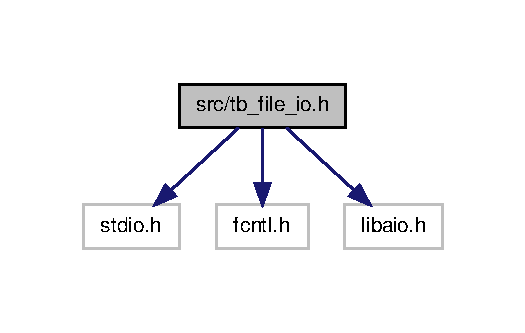
\includegraphics[width=252pt]{tb__file__io_8h__incl}
\end{center}
\end{figure}
This graph shows which files directly or indirectly include this file\-:\nopagebreak
\begin{figure}[H]
\begin{center}
\leavevmode
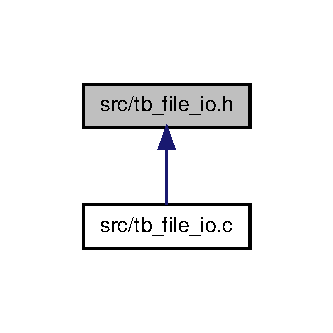
\includegraphics[width=160pt]{tb__file__io_8h__dep__incl}
\end{center}
\end{figure}
\subsection*{Data Structures}
\begin{DoxyCompactItemize}
\item 
struct \hyperlink{structtb__file__t}{tb\-\_\-file\-\_\-t}
\begin{DoxyCompactList}\small\item\em The struct that contains information about the file. \end{DoxyCompactList}\end{DoxyCompactItemize}
\subsection*{Enumerations}
\begin{DoxyCompactItemize}
\item 
enum \hyperlink{tb__file__io_8h_a365107762359ca7508e1b789f8f12c2b}{tb\-\_\-io\-\_\-type} \{ \hyperlink{tb__file__io_8h_a365107762359ca7508e1b789f8f12c2ba52d7a6f20bc89f3ba535f669297519b7}{I\-O\-\_\-\-S\-Y\-N\-C} =  0, 
\hyperlink{tb__file__io_8h_a365107762359ca7508e1b789f8f12c2ba02abfd86533a52a57456cc2b0d69493f}{I\-O\-\_\-\-B\-U\-F\-F\-\_\-\-S\-Y\-N\-C}, 
\hyperlink{tb__file__io_8h_a365107762359ca7508e1b789f8f12c2bad8d6dc6b2f348495288824d9ee2e9228}{I\-O\-\_\-\-A\-S\-Y\-N\-C}, 
\hyperlink{tb__file__io_8h_a365107762359ca7508e1b789f8f12c2ba6d286f9a1ec1698a582b1d5e929086e4}{I\-O\-\_\-\-M\-M\-A\-P}
 \}
\item 
enum \hyperlink{tb__file__io_8h_a6393ed40c2daaa55fe6411ff7b4a4e61}{tb\-\_\-o\-\_\-flags} \{ \hyperlink{tb__file__io_8h_a6393ed40c2daaa55fe6411ff7b4a4e61ae01aadd169d54a17dbfd96cda3c5d279}{R\-E\-A\-D\-\_\-\-W\-R\-I\-T\-E\-\_\-\-O\-N\-L\-Y} =  O\-\_\-\-R\-D\-W\-R, 
\hyperlink{tb__file__io_8h_a6393ed40c2daaa55fe6411ff7b4a4e61ae80b4cd4ef79e7e831a505a394d41857}{R\-E\-A\-D\-\_\-\-W\-R\-I\-T\-E\-\_\-\-C\-R\-E\-A\-T\-E} =  O\-\_\-\-R\-D\-W\-R $|$ O\-\_\-\-C\-R\-E\-A\-T
 \}
\end{DoxyCompactItemize}
\subsection*{Functions}
\begin{DoxyCompactItemize}
\item 
\hyperlink{structtb__file__t}{tb\-\_\-file\-\_\-t} $\ast$ \hyperlink{tb__file__io_8h_a8923d7ac413049b32a80b7d5bb4862bc}{tb\-\_\-setup\-\_\-mmap} (char $\ast$file\-\_\-path, \hyperlink{tb__file__io_8h_a6393ed40c2daaa55fe6411ff7b4a4e61}{tb\-\_\-o\-\_\-flags} flags, int file\-\_\-len)
\begin{DoxyCompactList}\small\item\em Setup mmap for io. \end{DoxyCompactList}\item 
int \hyperlink{tb__file__io_8h_ac261d5433c8e8ebb01207507d721b6af}{tb\-\_\-write\-\_\-mmap} (\hyperlink{structtb__file__t}{tb\-\_\-file\-\_\-t} $\ast$file, char $\ast$buff, int off, int len)
\begin{DoxyCompactList}\small\item\em Write to a file using mmap. \end{DoxyCompactList}\item 
int \hyperlink{tb__file__io_8h_a481feb547d00f86ef25abeed730fcaca}{tb\-\_\-read\-\_\-mmap} (\hyperlink{structtb__file__t}{tb\-\_\-file\-\_\-t} $\ast$file, char $\ast$buf, int off, int len)
\begin{DoxyCompactList}\small\item\em Read a file using mmap. \end{DoxyCompactList}\item 
int \hyperlink{tb__file__io_8h_a55a2fd2fc6edd2180d781b6a34582df9}{tb\-\_\-close\-\_\-mmap} (\hyperlink{structtb__file__t}{tb\-\_\-file\-\_\-t} $\ast$file)
\begin{DoxyCompactList}\small\item\em close mmap. \end{DoxyCompactList}\item 
\hyperlink{structtb__file__t}{tb\-\_\-file\-\_\-t} $\ast$ \hyperlink{tb__file__io_8h_a9f5f4287c8757462a0c0ad86864049a1}{tb\-\_\-setup\-\_\-s} (char $\ast$file\-\_\-path, \hyperlink{tb__file__io_8h_a6393ed40c2daaa55fe6411ff7b4a4e61}{tb\-\_\-o\-\_\-flags} flags, int file\-\_\-len)
\begin{DoxyCompactList}\small\item\em Setup for synchronous io. \end{DoxyCompactList}\item 
int \hyperlink{tb__file__io_8h_a49f736bb63ef24cca0dc00838fee96f4}{tb\-\_\-read\-\_\-s} (\hyperlink{structtb__file__t}{tb\-\_\-file\-\_\-t} $\ast$file, char $\ast$buf, int off, int len)
\begin{DoxyCompactList}\small\item\em Read a file synchronously. \end{DoxyCompactList}\item 
int \hyperlink{tb__file__io_8h_af7c9fa06df83c0f419e2b4aac6081298}{tb\-\_\-write\-\_\-s} (\hyperlink{structtb__file__t}{tb\-\_\-file\-\_\-t} $\ast$file, char $\ast$buf, int off, int len)
\begin{DoxyCompactList}\small\item\em Write to a file synchronously. \end{DoxyCompactList}\item 
int \hyperlink{tb__file__io_8h_a667112cc7e28387f256291eab00ace57}{tb\-\_\-close\-\_\-s} (\hyperlink{structtb__file__t}{tb\-\_\-file\-\_\-t} $\ast$file)
\begin{DoxyCompactList}\small\item\em Close for synchronous io. \end{DoxyCompactList}\item 
\hyperlink{structtb__file__t}{tb\-\_\-file\-\_\-t} $\ast$ \hyperlink{tb__file__io_8h_a9d820528f4e06a8a1f3e9698fb42e8c1}{tb\-\_\-setup\-\_\-buffs} (char $\ast$file\-\_\-path, \hyperlink{tb__file__io_8h_a6393ed40c2daaa55fe6411ff7b4a4e61}{tb\-\_\-o\-\_\-flags} flags, int file\-\_\-len)
\item 
int \hyperlink{tb__file__io_8h_a6c960255bd187281dee5391fd8752e02}{tb\-\_\-read\-\_\-buffs} (\hyperlink{structtb__file__t}{tb\-\_\-file\-\_\-t} $\ast$file, char $\ast$buf, int off, int len)
\item 
int \hyperlink{tb__file__io_8h_a7fddda8aa5dd31d0e828e1e19d895f64}{tb\-\_\-write\-\_\-buffs} (\hyperlink{structtb__file__t}{tb\-\_\-file\-\_\-t} $\ast$file, char $\ast$buf, int off, int len)
\item 
int \hyperlink{tb__file__io_8h_a3958f06dac0c99ad9868ec8911024738}{tb\-\_\-close\-\_\-buffs} (\hyperlink{structtb__file__t}{tb\-\_\-file\-\_\-t} $\ast$file)
\item 
\hyperlink{structtb__file__t}{tb\-\_\-file\-\_\-t} $\ast$ \hyperlink{tb__file__io_8h_a30bcba636e8426f96642f70abd11bddd}{tb\-\_\-setup\-\_\-as} (char $\ast$file\-\_\-path)
\begin{DoxyCompactList}\small\item\em Setup asynchronous io. \end{DoxyCompactList}\item 
int \hyperlink{tb__file__io_8h_ac057b3b466672d56324d1f005e62c91b}{tb\-\_\-read\-\_\-as} (\hyperlink{structtb__file__t}{tb\-\_\-file\-\_\-t} $\ast$file)
\begin{DoxyCompactList}\small\item\em Read a file asynchronously. \end{DoxyCompactList}\item 
int \hyperlink{tb__file__io_8h_a45134b687c7902939c6a3d07ae9422a7}{tb\-\_\-write\-\_\-as} (\hyperlink{structtb__file__t}{tb\-\_\-file\-\_\-t} $\ast$file)
\begin{DoxyCompactList}\small\item\em Write to a file asynchronously. \end{DoxyCompactList}\item 
int \hyperlink{tb__file__io_8h_aa936b3880e816db9b609f4949c4c281c}{tb\-\_\-close\-\_\-as} (\hyperlink{structtb__file__t}{tb\-\_\-file\-\_\-t} $\ast$file)
\begin{DoxyCompactList}\small\item\em Close asynchronous io. \end{DoxyCompactList}\end{DoxyCompactItemize}


\subsection{Enumeration Type Documentation}
\hypertarget{tb__file__io_8h_a365107762359ca7508e1b789f8f12c2b}{\index{tb\-\_\-file\-\_\-io.\-h@{tb\-\_\-file\-\_\-io.\-h}!tb\-\_\-io\-\_\-type@{tb\-\_\-io\-\_\-type}}
\index{tb\-\_\-io\-\_\-type@{tb\-\_\-io\-\_\-type}!tb_file_io.h@{tb\-\_\-file\-\_\-io.\-h}}
\subsubsection[{tb\-\_\-io\-\_\-type}]{\setlength{\rightskip}{0pt plus 5cm}enum {\bf tb\-\_\-io\-\_\-type}}}\label{tb__file__io_8h_a365107762359ca7508e1b789f8f12c2b}
\begin{Desc}
\item[Enumerator\-: ]\par
\begin{description}
\index{I\-O\-\_\-\-S\-Y\-N\-C@{I\-O\-\_\-\-S\-Y\-N\-C}!tb\-\_\-file\-\_\-io.\-h@{tb\-\_\-file\-\_\-io.\-h}}\index{tb\-\_\-file\-\_\-io.\-h@{tb\-\_\-file\-\_\-io.\-h}!I\-O\-\_\-\-S\-Y\-N\-C@{I\-O\-\_\-\-S\-Y\-N\-C}}\item[{\em 
\hypertarget{tb__file__io_8h_a365107762359ca7508e1b789f8f12c2ba52d7a6f20bc89f3ba535f669297519b7}{I\-O\-\_\-\-S\-Y\-N\-C}\label{tb__file__io_8h_a365107762359ca7508e1b789f8f12c2ba52d7a6f20bc89f3ba535f669297519b7}
}]\index{I\-O\-\_\-\-B\-U\-F\-F\-\_\-\-S\-Y\-N\-C@{I\-O\-\_\-\-B\-U\-F\-F\-\_\-\-S\-Y\-N\-C}!tb\-\_\-file\-\_\-io.\-h@{tb\-\_\-file\-\_\-io.\-h}}\index{tb\-\_\-file\-\_\-io.\-h@{tb\-\_\-file\-\_\-io.\-h}!I\-O\-\_\-\-B\-U\-F\-F\-\_\-\-S\-Y\-N\-C@{I\-O\-\_\-\-B\-U\-F\-F\-\_\-\-S\-Y\-N\-C}}\item[{\em 
\hypertarget{tb__file__io_8h_a365107762359ca7508e1b789f8f12c2ba02abfd86533a52a57456cc2b0d69493f}{I\-O\-\_\-\-B\-U\-F\-F\-\_\-\-S\-Y\-N\-C}\label{tb__file__io_8h_a365107762359ca7508e1b789f8f12c2ba02abfd86533a52a57456cc2b0d69493f}
}]\index{I\-O\-\_\-\-A\-S\-Y\-N\-C@{I\-O\-\_\-\-A\-S\-Y\-N\-C}!tb\-\_\-file\-\_\-io.\-h@{tb\-\_\-file\-\_\-io.\-h}}\index{tb\-\_\-file\-\_\-io.\-h@{tb\-\_\-file\-\_\-io.\-h}!I\-O\-\_\-\-A\-S\-Y\-N\-C@{I\-O\-\_\-\-A\-S\-Y\-N\-C}}\item[{\em 
\hypertarget{tb__file__io_8h_a365107762359ca7508e1b789f8f12c2bad8d6dc6b2f348495288824d9ee2e9228}{I\-O\-\_\-\-A\-S\-Y\-N\-C}\label{tb__file__io_8h_a365107762359ca7508e1b789f8f12c2bad8d6dc6b2f348495288824d9ee2e9228}
}]\index{I\-O\-\_\-\-M\-M\-A\-P@{I\-O\-\_\-\-M\-M\-A\-P}!tb\-\_\-file\-\_\-io.\-h@{tb\-\_\-file\-\_\-io.\-h}}\index{tb\-\_\-file\-\_\-io.\-h@{tb\-\_\-file\-\_\-io.\-h}!I\-O\-\_\-\-M\-M\-A\-P@{I\-O\-\_\-\-M\-M\-A\-P}}\item[{\em 
\hypertarget{tb__file__io_8h_a365107762359ca7508e1b789f8f12c2ba6d286f9a1ec1698a582b1d5e929086e4}{I\-O\-\_\-\-M\-M\-A\-P}\label{tb__file__io_8h_a365107762359ca7508e1b789f8f12c2ba6d286f9a1ec1698a582b1d5e929086e4}
}]\end{description}
\end{Desc}



Definition at line 21 of file tb\-\_\-file\-\_\-io.\-h.

\hypertarget{tb__file__io_8h_a6393ed40c2daaa55fe6411ff7b4a4e61}{\index{tb\-\_\-file\-\_\-io.\-h@{tb\-\_\-file\-\_\-io.\-h}!tb\-\_\-o\-\_\-flags@{tb\-\_\-o\-\_\-flags}}
\index{tb\-\_\-o\-\_\-flags@{tb\-\_\-o\-\_\-flags}!tb_file_io.h@{tb\-\_\-file\-\_\-io.\-h}}
\subsubsection[{tb\-\_\-o\-\_\-flags}]{\setlength{\rightskip}{0pt plus 5cm}enum {\bf tb\-\_\-o\-\_\-flags}}}\label{tb__file__io_8h_a6393ed40c2daaa55fe6411ff7b4a4e61}
\begin{Desc}
\item[Enumerator\-: ]\par
\begin{description}
\index{R\-E\-A\-D\-\_\-\-W\-R\-I\-T\-E\-\_\-\-O\-N\-L\-Y@{R\-E\-A\-D\-\_\-\-W\-R\-I\-T\-E\-\_\-\-O\-N\-L\-Y}!tb\-\_\-file\-\_\-io.\-h@{tb\-\_\-file\-\_\-io.\-h}}\index{tb\-\_\-file\-\_\-io.\-h@{tb\-\_\-file\-\_\-io.\-h}!R\-E\-A\-D\-\_\-\-W\-R\-I\-T\-E\-\_\-\-O\-N\-L\-Y@{R\-E\-A\-D\-\_\-\-W\-R\-I\-T\-E\-\_\-\-O\-N\-L\-Y}}\item[{\em 
\hypertarget{tb__file__io_8h_a6393ed40c2daaa55fe6411ff7b4a4e61ae01aadd169d54a17dbfd96cda3c5d279}{R\-E\-A\-D\-\_\-\-W\-R\-I\-T\-E\-\_\-\-O\-N\-L\-Y}\label{tb__file__io_8h_a6393ed40c2daaa55fe6411ff7b4a4e61ae01aadd169d54a17dbfd96cda3c5d279}
}]\index{R\-E\-A\-D\-\_\-\-W\-R\-I\-T\-E\-\_\-\-C\-R\-E\-A\-T\-E@{R\-E\-A\-D\-\_\-\-W\-R\-I\-T\-E\-\_\-\-C\-R\-E\-A\-T\-E}!tb\-\_\-file\-\_\-io.\-h@{tb\-\_\-file\-\_\-io.\-h}}\index{tb\-\_\-file\-\_\-io.\-h@{tb\-\_\-file\-\_\-io.\-h}!R\-E\-A\-D\-\_\-\-W\-R\-I\-T\-E\-\_\-\-C\-R\-E\-A\-T\-E@{R\-E\-A\-D\-\_\-\-W\-R\-I\-T\-E\-\_\-\-C\-R\-E\-A\-T\-E}}\item[{\em 
\hypertarget{tb__file__io_8h_a6393ed40c2daaa55fe6411ff7b4a4e61ae80b4cd4ef79e7e831a505a394d41857}{R\-E\-A\-D\-\_\-\-W\-R\-I\-T\-E\-\_\-\-C\-R\-E\-A\-T\-E}\label{tb__file__io_8h_a6393ed40c2daaa55fe6411ff7b4a4e61ae80b4cd4ef79e7e831a505a394d41857}
}]\end{description}
\end{Desc}



Definition at line 38 of file tb\-\_\-file\-\_\-io.\-h.



\subsection{Function Documentation}
\hypertarget{tb__file__io_8h_aa936b3880e816db9b609f4949c4c281c}{\index{tb\-\_\-file\-\_\-io.\-h@{tb\-\_\-file\-\_\-io.\-h}!tb\-\_\-close\-\_\-as@{tb\-\_\-close\-\_\-as}}
\index{tb\-\_\-close\-\_\-as@{tb\-\_\-close\-\_\-as}!tb_file_io.h@{tb\-\_\-file\-\_\-io.\-h}}
\subsubsection[{tb\-\_\-close\-\_\-as}]{\setlength{\rightskip}{0pt plus 5cm}int tb\-\_\-close\-\_\-as (
\begin{DoxyParamCaption}
\item[{{\bf tb\-\_\-file\-\_\-t} $\ast$}]{file}
\end{DoxyParamCaption}
)}}\label{tb__file__io_8h_aa936b3880e816db9b609f4949c4c281c}


Close asynchronous io. 



Definition at line 364 of file tb\-\_\-file\-\_\-io.\-c.

\hypertarget{tb__file__io_8h_a3958f06dac0c99ad9868ec8911024738}{\index{tb\-\_\-file\-\_\-io.\-h@{tb\-\_\-file\-\_\-io.\-h}!tb\-\_\-close\-\_\-buffs@{tb\-\_\-close\-\_\-buffs}}
\index{tb\-\_\-close\-\_\-buffs@{tb\-\_\-close\-\_\-buffs}!tb_file_io.h@{tb\-\_\-file\-\_\-io.\-h}}
\subsubsection[{tb\-\_\-close\-\_\-buffs}]{\setlength{\rightskip}{0pt plus 5cm}int tb\-\_\-close\-\_\-buffs (
\begin{DoxyParamCaption}
\item[{{\bf tb\-\_\-file\-\_\-t} $\ast$}]{file}
\end{DoxyParamCaption}
)}}\label{tb__file__io_8h_a3958f06dac0c99ad9868ec8911024738}


Definition at line 313 of file tb\-\_\-file\-\_\-io.\-c.

\hypertarget{tb__file__io_8h_a55a2fd2fc6edd2180d781b6a34582df9}{\index{tb\-\_\-file\-\_\-io.\-h@{tb\-\_\-file\-\_\-io.\-h}!tb\-\_\-close\-\_\-mmap@{tb\-\_\-close\-\_\-mmap}}
\index{tb\-\_\-close\-\_\-mmap@{tb\-\_\-close\-\_\-mmap}!tb_file_io.h@{tb\-\_\-file\-\_\-io.\-h}}
\subsubsection[{tb\-\_\-close\-\_\-mmap}]{\setlength{\rightskip}{0pt plus 5cm}int tb\-\_\-close\-\_\-mmap (
\begin{DoxyParamCaption}
\item[{{\bf tb\-\_\-file\-\_\-t} $\ast$}]{file}
\end{DoxyParamCaption}
)}}\label{tb__file__io_8h_a55a2fd2fc6edd2180d781b6a34582df9}


close mmap. 



Definition at line 139 of file tb\-\_\-file\-\_\-io.\-c.

\hypertarget{tb__file__io_8h_a667112cc7e28387f256291eab00ace57}{\index{tb\-\_\-file\-\_\-io.\-h@{tb\-\_\-file\-\_\-io.\-h}!tb\-\_\-close\-\_\-s@{tb\-\_\-close\-\_\-s}}
\index{tb\-\_\-close\-\_\-s@{tb\-\_\-close\-\_\-s}!tb_file_io.h@{tb\-\_\-file\-\_\-io.\-h}}
\subsubsection[{tb\-\_\-close\-\_\-s}]{\setlength{\rightskip}{0pt plus 5cm}int tb\-\_\-close\-\_\-s (
\begin{DoxyParamCaption}
\item[{{\bf tb\-\_\-file\-\_\-t} $\ast$}]{file}
\end{DoxyParamCaption}
)}}\label{tb__file__io_8h_a667112cc7e28387f256291eab00ace57}


Close for synchronous io. 



Definition at line 182 of file tb\-\_\-file\-\_\-io.\-c.

\hypertarget{tb__file__io_8h_ac057b3b466672d56324d1f005e62c91b}{\index{tb\-\_\-file\-\_\-io.\-h@{tb\-\_\-file\-\_\-io.\-h}!tb\-\_\-read\-\_\-as@{tb\-\_\-read\-\_\-as}}
\index{tb\-\_\-read\-\_\-as@{tb\-\_\-read\-\_\-as}!tb_file_io.h@{tb\-\_\-file\-\_\-io.\-h}}
\subsubsection[{tb\-\_\-read\-\_\-as}]{\setlength{\rightskip}{0pt plus 5cm}int tb\-\_\-read\-\_\-as (
\begin{DoxyParamCaption}
\item[{{\bf tb\-\_\-file\-\_\-t} $\ast$}]{file}
\end{DoxyParamCaption}
)}}\label{tb__file__io_8h_ac057b3b466672d56324d1f005e62c91b}


Read a file asynchronously. 



Definition at line 346 of file tb\-\_\-file\-\_\-io.\-c.

\hypertarget{tb__file__io_8h_a6c960255bd187281dee5391fd8752e02}{\index{tb\-\_\-file\-\_\-io.\-h@{tb\-\_\-file\-\_\-io.\-h}!tb\-\_\-read\-\_\-buffs@{tb\-\_\-read\-\_\-buffs}}
\index{tb\-\_\-read\-\_\-buffs@{tb\-\_\-read\-\_\-buffs}!tb_file_io.h@{tb\-\_\-file\-\_\-io.\-h}}
\subsubsection[{tb\-\_\-read\-\_\-buffs}]{\setlength{\rightskip}{0pt plus 5cm}int tb\-\_\-read\-\_\-buffs (
\begin{DoxyParamCaption}
\item[{{\bf tb\-\_\-file\-\_\-t} $\ast$}]{file, }
\item[{char $\ast$}]{buf, }
\item[{int}]{off, }
\item[{int}]{len}
\end{DoxyParamCaption}
)}}\label{tb__file__io_8h_a6c960255bd187281dee5391fd8752e02}


Definition at line 299 of file tb\-\_\-file\-\_\-io.\-c.

\hypertarget{tb__file__io_8h_a481feb547d00f86ef25abeed730fcaca}{\index{tb\-\_\-file\-\_\-io.\-h@{tb\-\_\-file\-\_\-io.\-h}!tb\-\_\-read\-\_\-mmap@{tb\-\_\-read\-\_\-mmap}}
\index{tb\-\_\-read\-\_\-mmap@{tb\-\_\-read\-\_\-mmap}!tb_file_io.h@{tb\-\_\-file\-\_\-io.\-h}}
\subsubsection[{tb\-\_\-read\-\_\-mmap}]{\setlength{\rightskip}{0pt plus 5cm}int tb\-\_\-read\-\_\-mmap (
\begin{DoxyParamCaption}
\item[{{\bf tb\-\_\-file\-\_\-t} $\ast$}]{file, }
\item[{char $\ast$}]{buf, }
\item[{int}]{off, }
\item[{int}]{len}
\end{DoxyParamCaption}
)}}\label{tb__file__io_8h_a481feb547d00f86ef25abeed730fcaca}


Read a file using mmap. 



Definition at line 128 of file tb\-\_\-file\-\_\-io.\-c.

\hypertarget{tb__file__io_8h_a49f736bb63ef24cca0dc00838fee96f4}{\index{tb\-\_\-file\-\_\-io.\-h@{tb\-\_\-file\-\_\-io.\-h}!tb\-\_\-read\-\_\-s@{tb\-\_\-read\-\_\-s}}
\index{tb\-\_\-read\-\_\-s@{tb\-\_\-read\-\_\-s}!tb_file_io.h@{tb\-\_\-file\-\_\-io.\-h}}
\subsubsection[{tb\-\_\-read\-\_\-s}]{\setlength{\rightskip}{0pt plus 5cm}int tb\-\_\-read\-\_\-s (
\begin{DoxyParamCaption}
\item[{{\bf tb\-\_\-file\-\_\-t} $\ast$}]{file, }
\item[{char $\ast$}]{buf, }
\item[{int}]{off, }
\item[{int}]{len}
\end{DoxyParamCaption}
)}}\label{tb__file__io_8h_a49f736bb63ef24cca0dc00838fee96f4}


Read a file synchronously. 



Definition at line 193 of file tb\-\_\-file\-\_\-io.\-c.

\hypertarget{tb__file__io_8h_a30bcba636e8426f96642f70abd11bddd}{\index{tb\-\_\-file\-\_\-io.\-h@{tb\-\_\-file\-\_\-io.\-h}!tb\-\_\-setup\-\_\-as@{tb\-\_\-setup\-\_\-as}}
\index{tb\-\_\-setup\-\_\-as@{tb\-\_\-setup\-\_\-as}!tb_file_io.h@{tb\-\_\-file\-\_\-io.\-h}}
\subsubsection[{tb\-\_\-setup\-\_\-as}]{\setlength{\rightskip}{0pt plus 5cm}{\bf tb\-\_\-file\-\_\-t}$\ast$ tb\-\_\-setup\-\_\-as (
\begin{DoxyParamCaption}
\item[{char $\ast$}]{file\-\_\-path}
\end{DoxyParamCaption}
)}}\label{tb__file__io_8h_a30bcba636e8426f96642f70abd11bddd}


Setup asynchronous io. 



Definition at line 325 of file tb\-\_\-file\-\_\-io.\-c.

\hypertarget{tb__file__io_8h_a9d820528f4e06a8a1f3e9698fb42e8c1}{\index{tb\-\_\-file\-\_\-io.\-h@{tb\-\_\-file\-\_\-io.\-h}!tb\-\_\-setup\-\_\-buffs@{tb\-\_\-setup\-\_\-buffs}}
\index{tb\-\_\-setup\-\_\-buffs@{tb\-\_\-setup\-\_\-buffs}!tb_file_io.h@{tb\-\_\-file\-\_\-io.\-h}}
\subsubsection[{tb\-\_\-setup\-\_\-buffs}]{\setlength{\rightskip}{0pt plus 5cm}{\bf tb\-\_\-file\-\_\-t}$\ast$ tb\-\_\-setup\-\_\-buffs (
\begin{DoxyParamCaption}
\item[{char $\ast$}]{file\-\_\-path, }
\item[{{\bf tb\-\_\-o\-\_\-flags}}]{flags, }
\item[{int}]{file\-\_\-len}
\end{DoxyParamCaption}
)}}\label{tb__file__io_8h_a9d820528f4e06a8a1f3e9698fb42e8c1}


Definition at line 232 of file tb\-\_\-file\-\_\-io.\-c.

\hypertarget{tb__file__io_8h_a8923d7ac413049b32a80b7d5bb4862bc}{\index{tb\-\_\-file\-\_\-io.\-h@{tb\-\_\-file\-\_\-io.\-h}!tb\-\_\-setup\-\_\-mmap@{tb\-\_\-setup\-\_\-mmap}}
\index{tb\-\_\-setup\-\_\-mmap@{tb\-\_\-setup\-\_\-mmap}!tb_file_io.h@{tb\-\_\-file\-\_\-io.\-h}}
\subsubsection[{tb\-\_\-setup\-\_\-mmap}]{\setlength{\rightskip}{0pt plus 5cm}{\bf tb\-\_\-file\-\_\-t}$\ast$ tb\-\_\-setup\-\_\-mmap (
\begin{DoxyParamCaption}
\item[{char $\ast$}]{file\-\_\-path, }
\item[{{\bf tb\-\_\-o\-\_\-flags}}]{flags, }
\item[{int}]{file\-\_\-len}
\end{DoxyParamCaption}
)}}\label{tb__file__io_8h_a8923d7ac413049b32a80b7d5bb4862bc}


Setup mmap for io. 



Definition at line 66 of file tb\-\_\-file\-\_\-io.\-c.

\hypertarget{tb__file__io_8h_a9f5f4287c8757462a0c0ad86864049a1}{\index{tb\-\_\-file\-\_\-io.\-h@{tb\-\_\-file\-\_\-io.\-h}!tb\-\_\-setup\-\_\-s@{tb\-\_\-setup\-\_\-s}}
\index{tb\-\_\-setup\-\_\-s@{tb\-\_\-setup\-\_\-s}!tb_file_io.h@{tb\-\_\-file\-\_\-io.\-h}}
\subsubsection[{tb\-\_\-setup\-\_\-s}]{\setlength{\rightskip}{0pt plus 5cm}{\bf tb\-\_\-file\-\_\-t}$\ast$ tb\-\_\-setup\-\_\-s (
\begin{DoxyParamCaption}
\item[{char $\ast$}]{file\-\_\-path, }
\item[{{\bf tb\-\_\-o\-\_\-flags}}]{flags, }
\item[{int}]{file\-\_\-len}
\end{DoxyParamCaption}
)}}\label{tb__file__io_8h_a9f5f4287c8757462a0c0ad86864049a1}


Setup for synchronous io. 



Definition at line 151 of file tb\-\_\-file\-\_\-io.\-c.

\hypertarget{tb__file__io_8h_a45134b687c7902939c6a3d07ae9422a7}{\index{tb\-\_\-file\-\_\-io.\-h@{tb\-\_\-file\-\_\-io.\-h}!tb\-\_\-write\-\_\-as@{tb\-\_\-write\-\_\-as}}
\index{tb\-\_\-write\-\_\-as@{tb\-\_\-write\-\_\-as}!tb_file_io.h@{tb\-\_\-file\-\_\-io.\-h}}
\subsubsection[{tb\-\_\-write\-\_\-as}]{\setlength{\rightskip}{0pt plus 5cm}int tb\-\_\-write\-\_\-as (
\begin{DoxyParamCaption}
\item[{{\bf tb\-\_\-file\-\_\-t} $\ast$}]{file}
\end{DoxyParamCaption}
)}}\label{tb__file__io_8h_a45134b687c7902939c6a3d07ae9422a7}


Write to a file asynchronously. 



Definition at line 355 of file tb\-\_\-file\-\_\-io.\-c.

\hypertarget{tb__file__io_8h_a7fddda8aa5dd31d0e828e1e19d895f64}{\index{tb\-\_\-file\-\_\-io.\-h@{tb\-\_\-file\-\_\-io.\-h}!tb\-\_\-write\-\_\-buffs@{tb\-\_\-write\-\_\-buffs}}
\index{tb\-\_\-write\-\_\-buffs@{tb\-\_\-write\-\_\-buffs}!tb_file_io.h@{tb\-\_\-file\-\_\-io.\-h}}
\subsubsection[{tb\-\_\-write\-\_\-buffs}]{\setlength{\rightskip}{0pt plus 5cm}int tb\-\_\-write\-\_\-buffs (
\begin{DoxyParamCaption}
\item[{{\bf tb\-\_\-file\-\_\-t} $\ast$}]{file, }
\item[{char $\ast$}]{buf, }
\item[{int}]{off, }
\item[{int}]{len}
\end{DoxyParamCaption}
)}}\label{tb__file__io_8h_a7fddda8aa5dd31d0e828e1e19d895f64}


Definition at line 285 of file tb\-\_\-file\-\_\-io.\-c.

\hypertarget{tb__file__io_8h_ac261d5433c8e8ebb01207507d721b6af}{\index{tb\-\_\-file\-\_\-io.\-h@{tb\-\_\-file\-\_\-io.\-h}!tb\-\_\-write\-\_\-mmap@{tb\-\_\-write\-\_\-mmap}}
\index{tb\-\_\-write\-\_\-mmap@{tb\-\_\-write\-\_\-mmap}!tb_file_io.h@{tb\-\_\-file\-\_\-io.\-h}}
\subsubsection[{tb\-\_\-write\-\_\-mmap}]{\setlength{\rightskip}{0pt plus 5cm}int tb\-\_\-write\-\_\-mmap (
\begin{DoxyParamCaption}
\item[{{\bf tb\-\_\-file\-\_\-t} $\ast$}]{file, }
\item[{char $\ast$}]{buff, }
\item[{int}]{off, }
\item[{int}]{len}
\end{DoxyParamCaption}
)}}\label{tb__file__io_8h_ac261d5433c8e8ebb01207507d721b6af}


Write to a file using mmap. 



Definition at line 117 of file tb\-\_\-file\-\_\-io.\-c.

\hypertarget{tb__file__io_8h_af7c9fa06df83c0f419e2b4aac6081298}{\index{tb\-\_\-file\-\_\-io.\-h@{tb\-\_\-file\-\_\-io.\-h}!tb\-\_\-write\-\_\-s@{tb\-\_\-write\-\_\-s}}
\index{tb\-\_\-write\-\_\-s@{tb\-\_\-write\-\_\-s}!tb_file_io.h@{tb\-\_\-file\-\_\-io.\-h}}
\subsubsection[{tb\-\_\-write\-\_\-s}]{\setlength{\rightskip}{0pt plus 5cm}int tb\-\_\-write\-\_\-s (
\begin{DoxyParamCaption}
\item[{{\bf tb\-\_\-file\-\_\-t} $\ast$}]{file, }
\item[{char $\ast$}]{buf, }
\item[{int}]{off, }
\item[{int}]{len}
\end{DoxyParamCaption}
)}}\label{tb__file__io_8h_af7c9fa06df83c0f419e2b4aac6081298}


Write to a file synchronously. 



Definition at line 214 of file tb\-\_\-file\-\_\-io.\-c.


\hypertarget{tb__listener_8c}{\section{src/tb\-\_\-listener.c File Reference}
\label{tb__listener_8c}\index{src/tb\-\_\-listener.\-c@{src/tb\-\_\-listener.\-c}}
}
{\ttfamily \#include \char`\"{}tb\-\_\-listener.\-h\char`\"{}}\\*
{\ttfamily \#include \char`\"{}tb\-\_\-worker\-\_\-pair.\-h\char`\"{}}\\*
{\ttfamily \#include \char`\"{}tb\-\_\-protocol.\-h\char`\"{}}\\*
{\ttfamily \#include \char`\"{}tb\-\_\-common.\-h\char`\"{}}\\*
{\ttfamily \#include \char`\"{}tb\-\_\-worker.\-h\char`\"{}}\\*
{\ttfamily \#include \char`\"{}tb\-\_\-logging.\-h\char`\"{}}\\*
{\ttfamily \#include \char`\"{}tb\-\_\-sock\-\_\-opt.\-h\char`\"{}}\\*
{\ttfamily \#include \char`\"{}tb\-\_\-session.\-h\char`\"{}}\\*
{\ttfamily \#include $<$gdsl/gdsl\-\_\-heap.\-h$>$}\\*
{\ttfamily \#include $<$gdsl/gdsl\-\_\-hash.\-h$>$}\\*
{\ttfamily \#include $<$stdlib.\-h$>$}\\*
{\ttfamily \#include $<$pthread.\-h$>$}\\*
{\ttfamily \#include $<$sys/socket.\-h$>$}\\*
{\ttfamily \#include $<$string.\-h$>$}\\*
{\ttfamily \#include $<$netdb.\-h$>$}\\*
{\ttfamily \#include $<$errno.\-h$>$}\\*
{\ttfamily \#include $<$fcntl.\-h$>$}\\*
{\ttfamily \#include $<$sys/epoll.\-h$>$}\\*
{\ttfamily \#include $<$udt.\-h$>$}\\*
{\ttfamily \#include $<$assert.\-h$>$}\\*
{\ttfamily \#include $<$unistd.\-h$>$}\\*
{\ttfamily \#include $<$sys/syscall.\-h$>$}\\*
{\ttfamily \#include $<$sys/sysinfo.\-h$>$}\\*
{\ttfamily \#include $<$glib-\/2.\-0/glib.\-h$>$}\\*
Include dependency graph for tb\-\_\-listener.\-c\-:\nopagebreak
\begin{figure}[H]
\begin{center}
\leavevmode
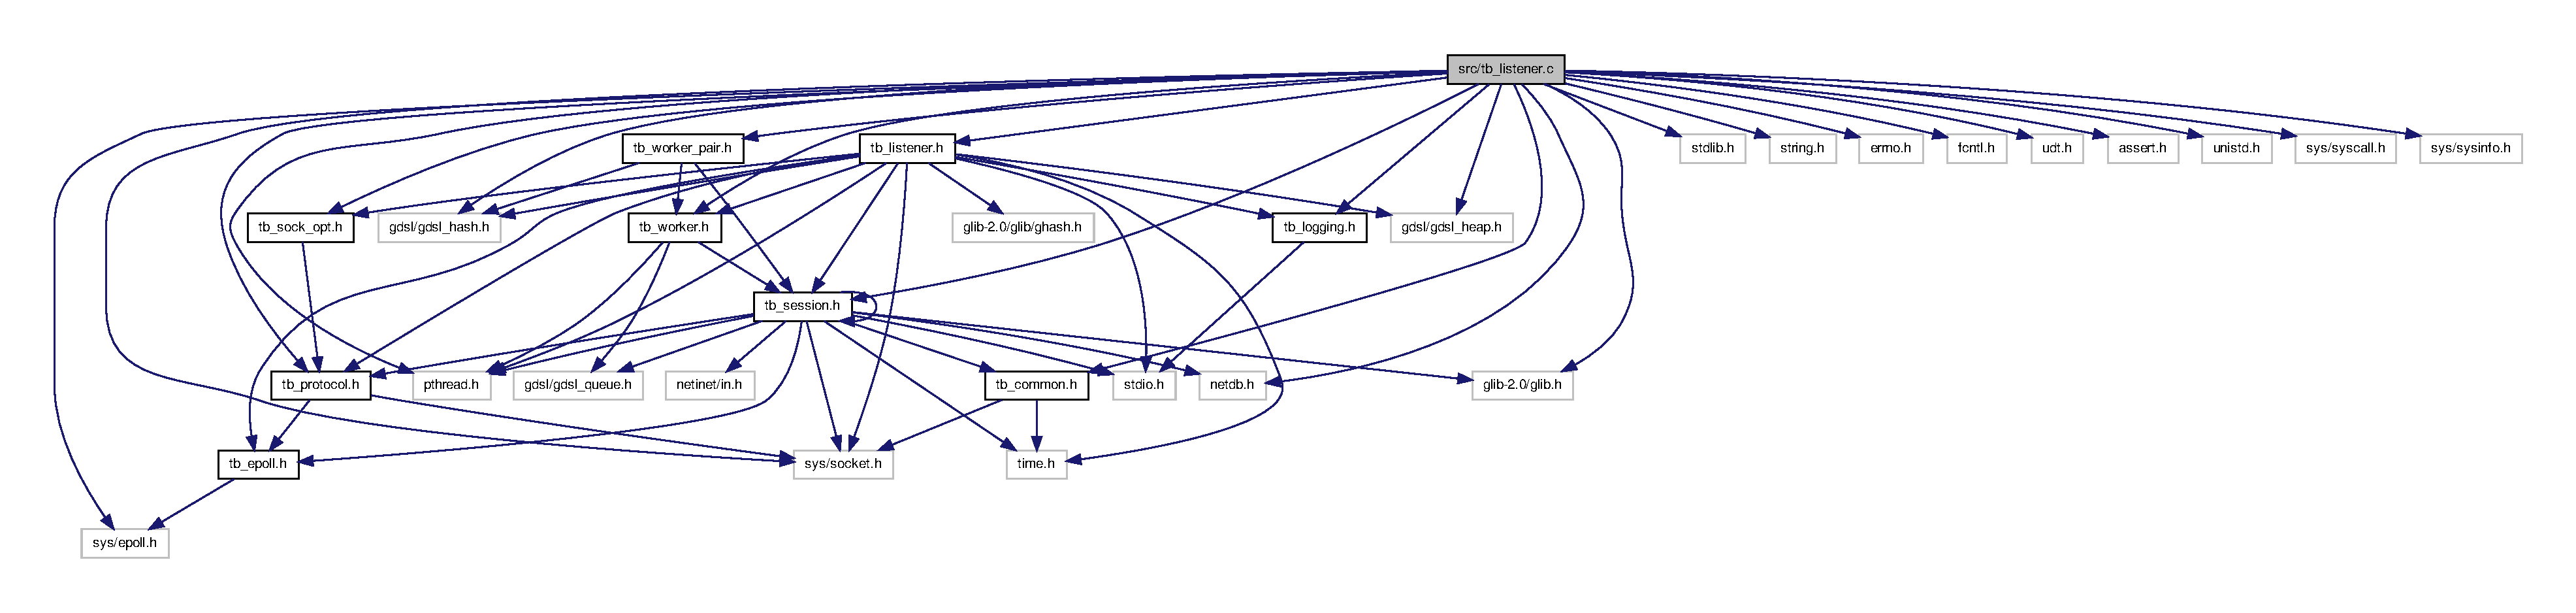
\includegraphics[width=350pt]{tb__listener_8c__incl}
\end{center}
\end{figure}
\subsection*{Functions}
\begin{DoxyCompactItemize}
\item 
\hyperlink{structtb__listener__t}{tb\-\_\-listener\-\_\-t} $\ast$ \hyperlink{tb__listener_8c_a5ec3b6c120621050965582e51e4d0d5a}{tb\-\_\-create\-\_\-listener} (\hyperlink{tb__listener_8h_ae37f3ebcf0081b2dd11adf41f1f867d6}{E\-N\-D\-P\-O\-I\-N\-T\-\_\-\-T\-Y\-P\-E} type, char $\ast$addr, char $\ast$port, \hyperlink{tb__protocol_8h_a7a5bff1040fc154c510874327d44cc1a}{P\-R\-O\-T\-O\-C\-O\-L} protocol, int bufsize)
\begin{DoxyCompactList}\small\item\em Create a listener with the supplied parameters. \end{DoxyCompactList}\item 
\hyperlink{structtb__listener__t}{tb\-\_\-listener\-\_\-t} $\ast$ \hyperlink{tb__listener_8c_a042a2b565ccc70e1506562ad43c83bfb}{tb\-\_\-create\-\_\-endpoint} (\hyperlink{structtb__test__params__t}{tb\-\_\-test\-\_\-params\-\_\-t} $\ast$params)
\begin{DoxyCompactList}\small\item\em Create a listener using a \hyperlink{structtb__test__params__t}{tb\-\_\-test\-\_\-params\-\_\-t} struct. \end{DoxyCompactList}\item 
int \hyperlink{tb__listener_8c_a104d49d9fbeed470cf0a9de8706c0af8}{tb\-\_\-setup\-\_\-workers} (\hyperlink{structtb__listener__t}{tb\-\_\-listener\-\_\-t} $\ast$listener, int num\-\_\-threads)
\item 
\hyperlink{structtb__worker__t}{tb\-\_\-worker\-\_\-t} $\ast$ \hyperlink{tb__listener_8c_aadc6c1af686cf9fc7bbd8874eca3be42}{tb\-\_\-get\-\_\-worker} (\hyperlink{structtb__listener__t}{tb\-\_\-listener\-\_\-t} $\ast$listener, \hyperlink{structtb__session__t}{tb\-\_\-session\-\_\-t} $\ast$session)
\begin{DoxyCompactList}\small\item\em Get a worker for the supplied session. \end{DoxyCompactList}\item 
\hyperlink{structtb__worker__t}{tb\-\_\-worker\-\_\-t} $\ast$ \hyperlink{tb__listener_8c_a215355da81075fa189618103a0bfb916}{tb\-\_\-get\-\_\-session} (\hyperlink{structtb__listener__t}{tb\-\_\-listener\-\_\-t} $\ast$listener, \hyperlink{structtb__session__t}{tb\-\_\-session\-\_\-t} $\ast$session)
\item 
void \hyperlink{tb__listener_8c_aa1646d6df4318c903d2653a6032a0a40}{tb\-\_\-get\-\_\-cpu\-\_\-info} (\hyperlink{structtb__listener__t}{tb\-\_\-listener\-\_\-t} $\ast$listener)
\item 
void \hyperlink{tb__listener_8c_a370d0eb443de6db87ab002ea2e5cc468}{tb\-\_\-destroy\-\_\-listener} (\hyperlink{structtb__listener__t}{tb\-\_\-listener\-\_\-t} $\ast$listener)
\begin{DoxyCompactList}\small\item\em Destroy a listener. \end{DoxyCompactList}\item 
void \hyperlink{tb__listener_8c_af552255cac39c1b712a1c213070c04e0}{tb\-\_\-print\-\_\-listener} (\hyperlink{structtb__listener__t}{tb\-\_\-listener\-\_\-t} $\ast$listener)
\begin{DoxyCompactList}\small\item\em Print a listener. \end{DoxyCompactList}\item 
\hyperlink{structtb__prot__stats__t}{tb\-\_\-prot\-\_\-stats\-\_\-t} $\ast$ \hyperlink{tb__listener_8c_a6e5c88a915882ea9d39fd41ee4742ffc}{tb\-\_\-ex\-\_\-get\-\_\-stats} (\hyperlink{structtb__listener__t}{tb\-\_\-listener\-\_\-t} $\ast$listener)
\begin{DoxyCompactList}\small\item\em A thread safe way to get access to stats. \end{DoxyCompactList}\item 
void \hyperlink{tb__listener_8c_ae063a1fdce497a4e08aea504a6ab927b}{tb\-\_\-set\-\_\-l\-\_\-stats} (\hyperlink{structtb__listener__t}{tb\-\_\-listener\-\_\-t} $\ast$listener)
\begin{DoxyCompactList}\small\item\em Gets the stats for the listener. \end{DoxyCompactList}\item 
void \hyperlink{tb__listener_8c_a144e59e2470a90fc2b6e1f840da77ae8}{tb\-\_\-set\-\_\-m\-\_\-stats} (\hyperlink{structtb__listener__t}{tb\-\_\-listener\-\_\-t} $\ast$listener)
\begin{DoxyCompactList}\small\item\em Gets the stats for the listener. \end{DoxyCompactList}\item 
int \hyperlink{tb__listener_8c_a05130f296853ae0e2d00aee025f6773a}{tb\-\_\-listen} (\hyperlink{structtb__listener__t}{tb\-\_\-listener\-\_\-t} $\ast$listener)
\begin{DoxyCompactList}\small\item\em Bind and listen. \end{DoxyCompactList}\item 
\hyperlink{structtb__session__t}{tb\-\_\-session\-\_\-t} $\ast$ \hyperlink{tb__listener_8c_a8a79bda6c64046a1b527e045c9487ac8}{tb\-\_\-accept} (\hyperlink{structtb__listener__t}{tb\-\_\-listener\-\_\-t} $\ast$listener)
\begin{DoxyCompactList}\small\item\em Accept an incoming connection. \end{DoxyCompactList}\item 
\hyperlink{structtb__session__t}{tb\-\_\-session\-\_\-t} $\ast$ \hyperlink{tb__listener_8c_adeff1eb694f2649f6e9452ebbab990c4}{tb\-\_\-epoll\-\_\-accept} (\hyperlink{structtb__listener__t}{tb\-\_\-listener\-\_\-t} $\ast$listener)
\item 
int \hyperlink{tb__listener_8c_aedd19f27c5b2e1d8717024afed30ec51}{tb\-\_\-resolve\-\_\-address} (\hyperlink{structtb__listener__t}{tb\-\_\-listener\-\_\-t} $\ast$listener)
\begin{DoxyCompactList}\small\item\em Resolve the address for the given listener. \end{DoxyCompactList}\item 
int \hyperlink{tb__listener_8c_a453c35ddb0c42f1ecd1b963e7945860f}{tb\-\_\-create\-\_\-socket} (\hyperlink{structtb__listener__t}{tb\-\_\-listener\-\_\-t} $\ast$listener)
\begin{DoxyCompactList}\small\item\em Create a socket. \end{DoxyCompactList}\item 
int \hyperlink{tb__listener_8c_afd4a201df5fe1e9b2e8a694ac270255a}{tb\-\_\-connect} (\hyperlink{structtb__listener__t}{tb\-\_\-listener\-\_\-t} $\ast$listener)
\begin{DoxyCompactList}\small\item\em Attempt to connect. \end{DoxyCompactList}\item 
int \hyperlink{tb__listener_8c_a26cdc218a6e64bb4afeb7751752a806a}{tb\-\_\-bind} (\hyperlink{structtb__listener__t}{tb\-\_\-listener\-\_\-t} $\ast$listener)
\begin{DoxyCompactList}\small\item\em Bind the listener to its address. \end{DoxyCompactList}\item 
int \hyperlink{tb__listener_8c_a259b174a6102fa292d1fd63125cb3035}{tb\-\_\-send\-\_\-data} (\hyperlink{structtb__listener__t}{tb\-\_\-listener\-\_\-t} $\ast$listener, char $\ast$buff, int size)
\begin{DoxyCompactList}\small\item\em Send data. \end{DoxyCompactList}\item 
int \hyperlink{tb__listener_8c_a2456170f46148e20d6e87110db95c89c}{tb\-\_\-recv\-\_\-data} (\hyperlink{structtb__listener__t}{tb\-\_\-listener\-\_\-t} $\ast$listener, \hyperlink{structtb__session__t}{tb\-\_\-session\-\_\-t} $\ast$session)
\begin{DoxyCompactList}\small\item\em Receive data. \end{DoxyCompactList}\item 
int \hyperlink{tb__listener_8c_ab66b3e6da7a5d6df6e36eaefda0a8463}{tb\-\_\-send\-\_\-to} (\hyperlink{structtb__listener__t}{tb\-\_\-listener\-\_\-t} $\ast$listener, \hyperlink{structtb__session__t}{tb\-\_\-session\-\_\-t} $\ast$session)
\item 
int \hyperlink{tb__listener_8c_aeeb4e0453d1d48ce53d354b836fa0706}{tb\-\_\-recv\-\_\-from} (\hyperlink{structtb__listener__t}{tb\-\_\-listener\-\_\-t} $\ast$listener, \hyperlink{structtb__session__t}{tb\-\_\-session\-\_\-t} $\ast$session)
\begin{DoxyCompactList}\small\item\em recv from -\/ used by U\-D\-P. \end{DoxyCompactList}\item 
int \hyperlink{tb__listener_8c_a51ee3fc570bf367b96f646a4d15f313d}{tb\-\_\-set\-\_\-epoll} (\hyperlink{structtb__listener__t}{tb\-\_\-listener\-\_\-t} $\ast$listener)
\begin{DoxyCompactList}\small\item\em Set epoll for this listener. \end{DoxyCompactList}\item 
void \hyperlink{tb__listener_8c_aca070e070aa077fd83fda3d2f448bfca}{tb\-\_\-error} (\hyperlink{structtb__listener__t}{tb\-\_\-listener\-\_\-t} $\ast$listener, const char $\ast$info, int err\-\_\-no)
\begin{DoxyCompactList}\small\item\em Format an error to the log file. \end{DoxyCompactList}\item 
void \hyperlink{tb__listener_8c_a1a5b9849075e44703d7815be5934af11}{tb\-\_\-address} (\hyperlink{structtb__listener__t}{tb\-\_\-listener\-\_\-t} $\ast$listener, const char $\ast$info, struct sockaddr\-\_\-storage $\ast$store)
\end{DoxyCompactItemize}


\subsection{Function Documentation}
\hypertarget{tb__listener_8c_a8a79bda6c64046a1b527e045c9487ac8}{\index{tb\-\_\-listener.\-c@{tb\-\_\-listener.\-c}!tb\-\_\-accept@{tb\-\_\-accept}}
\index{tb\-\_\-accept@{tb\-\_\-accept}!tb_listener.c@{tb\-\_\-listener.\-c}}
\subsubsection[{tb\-\_\-accept}]{\setlength{\rightskip}{0pt plus 5cm}{\bf tb\-\_\-session\-\_\-t}$\ast$ tb\-\_\-accept (
\begin{DoxyParamCaption}
\item[{{\bf tb\-\_\-listener\-\_\-t} $\ast$}]{listener}
\end{DoxyParamCaption}
)\hspace{0.3cm}{\ttfamily [inline]}}}\label{tb__listener_8c_a8a79bda6c64046a1b527e045c9487ac8}


Accept an incoming connection. 

Accepts incoming connections. This operation blocks, as we are using blocking I/\-O currently


\begin{DoxyParams}{Parameters}
{\em listener} & The listener to accept the connection on. \\
\hline
\end{DoxyParams}
\begin{DoxyReturn}{Returns}
\hyperlink{structtb__session__t}{tb\-\_\-session\-\_\-t} A newly created session. 
\end{DoxyReturn}


Definition at line 466 of file tb\-\_\-listener.\-c.

\hypertarget{tb__listener_8c_a1a5b9849075e44703d7815be5934af11}{\index{tb\-\_\-listener.\-c@{tb\-\_\-listener.\-c}!tb\-\_\-address@{tb\-\_\-address}}
\index{tb\-\_\-address@{tb\-\_\-address}!tb_listener.c@{tb\-\_\-listener.\-c}}
\subsubsection[{tb\-\_\-address}]{\setlength{\rightskip}{0pt plus 5cm}void tb\-\_\-address (
\begin{DoxyParamCaption}
\item[{{\bf tb\-\_\-listener\-\_\-t} $\ast$}]{listener, }
\item[{const char $\ast$}]{info, }
\item[{struct sockaddr\-\_\-storage $\ast$}]{store}
\end{DoxyParamCaption}
)\hspace{0.3cm}{\ttfamily [inline]}}}\label{tb__listener_8c_a1a5b9849075e44703d7815be5934af11}


Definition at line 692 of file tb\-\_\-listener.\-c.

\hypertarget{tb__listener_8c_a26cdc218a6e64bb4afeb7751752a806a}{\index{tb\-\_\-listener.\-c@{tb\-\_\-listener.\-c}!tb\-\_\-bind@{tb\-\_\-bind}}
\index{tb\-\_\-bind@{tb\-\_\-bind}!tb_listener.c@{tb\-\_\-listener.\-c}}
\subsubsection[{tb\-\_\-bind}]{\setlength{\rightskip}{0pt plus 5cm}int tb\-\_\-bind (
\begin{DoxyParamCaption}
\item[{{\bf tb\-\_\-listener\-\_\-t} $\ast$}]{listener}
\end{DoxyParamCaption}
)\hspace{0.3cm}{\ttfamily [inline]}}}\label{tb__listener_8c_a26cdc218a6e64bb4afeb7751752a806a}


Bind the listener to its address. 

Binds the listener to the address specified by address.


\begin{DoxyParams}{Parameters}
{\em listener} & The listener to bind. \\
\hline
\end{DoxyParams}
\begin{DoxyReturn}{Returns}
0 on success, -\/1 on failure. 
\end{DoxyReturn}


Definition at line 564 of file tb\-\_\-listener.\-c.

\hypertarget{tb__listener_8c_afd4a201df5fe1e9b2e8a694ac270255a}{\index{tb\-\_\-listener.\-c@{tb\-\_\-listener.\-c}!tb\-\_\-connect@{tb\-\_\-connect}}
\index{tb\-\_\-connect@{tb\-\_\-connect}!tb_listener.c@{tb\-\_\-listener.\-c}}
\subsubsection[{tb\-\_\-connect}]{\setlength{\rightskip}{0pt plus 5cm}int tb\-\_\-connect (
\begin{DoxyParamCaption}
\item[{{\bf tb\-\_\-listener\-\_\-t} $\ast$}]{listener}
\end{DoxyParamCaption}
)\hspace{0.3cm}{\ttfamily [inline]}}}\label{tb__listener_8c_afd4a201df5fe1e9b2e8a694ac270255a}


Attempt to connect. 

Attempts to connect to the specified address and port. 

Definition at line 545 of file tb\-\_\-listener.\-c.

\hypertarget{tb__listener_8c_a042a2b565ccc70e1506562ad43c83bfb}{\index{tb\-\_\-listener.\-c@{tb\-\_\-listener.\-c}!tb\-\_\-create\-\_\-endpoint@{tb\-\_\-create\-\_\-endpoint}}
\index{tb\-\_\-create\-\_\-endpoint@{tb\-\_\-create\-\_\-endpoint}!tb_listener.c@{tb\-\_\-listener.\-c}}
\subsubsection[{tb\-\_\-create\-\_\-endpoint}]{\setlength{\rightskip}{0pt plus 5cm}{\bf tb\-\_\-listener\-\_\-t}$\ast$ tb\-\_\-create\-\_\-endpoint (
\begin{DoxyParamCaption}
\item[{{\bf tb\-\_\-test\-\_\-params\-\_\-t} $\ast$}]{params}
\end{DoxyParamCaption}
)}}\label{tb__listener_8c_a042a2b565ccc70e1506562ad43c83bfb}


Create a listener using a \hyperlink{structtb__test__params__t}{tb\-\_\-test\-\_\-params\-\_\-t} struct. 

The details in the struct are used to create an endpoint for use in testing.


\begin{DoxyParams}{Parameters}
{\em params} & A struct with all of the required details for a test. \\
\hline
\end{DoxyParams}
\begin{DoxyReturn}{Returns}
the endpoint to test with. 
\end{DoxyReturn}


Definition at line 158 of file tb\-\_\-listener.\-c.

\hypertarget{tb__listener_8c_a5ec3b6c120621050965582e51e4d0d5a}{\index{tb\-\_\-listener.\-c@{tb\-\_\-listener.\-c}!tb\-\_\-create\-\_\-listener@{tb\-\_\-create\-\_\-listener}}
\index{tb\-\_\-create\-\_\-listener@{tb\-\_\-create\-\_\-listener}!tb_listener.c@{tb\-\_\-listener.\-c}}
\subsubsection[{tb\-\_\-create\-\_\-listener}]{\setlength{\rightskip}{0pt plus 5cm}{\bf tb\-\_\-listener\-\_\-t}$\ast$ tb\-\_\-create\-\_\-listener (
\begin{DoxyParamCaption}
\item[{{\bf E\-N\-D\-P\-O\-I\-N\-T\-\_\-\-T\-Y\-P\-E}}]{type, }
\item[{char $\ast$}]{addr, }
\item[{char $\ast$}]{port, }
\item[{{\bf P\-R\-O\-T\-O\-C\-O\-L}}]{protocol, }
\item[{int}]{bufsize}
\end{DoxyParamCaption}
)}}\label{tb__listener_8c_a5ec3b6c120621050965582e51e4d0d5a}


Create a listener with the supplied parameters. 

Creates a listener and the accociated data structures.


\begin{DoxyParams}{Parameters}
{\em type} & The type of endpoint to create. \\
\hline
{\em addr} & The address to bind to. \\
\hline
{\em port} & The port to bind to. \\
\hline
{\em num\-\_\-threads} & The number of worker threads to use.\\
\hline
\end{DoxyParams}
\begin{DoxyReturn}{Returns}
The newly created listener. 
\end{DoxyReturn}


Definition at line 38 of file tb\-\_\-listener.\-c.

\hypertarget{tb__listener_8c_a453c35ddb0c42f1ecd1b963e7945860f}{\index{tb\-\_\-listener.\-c@{tb\-\_\-listener.\-c}!tb\-\_\-create\-\_\-socket@{tb\-\_\-create\-\_\-socket}}
\index{tb\-\_\-create\-\_\-socket@{tb\-\_\-create\-\_\-socket}!tb_listener.c@{tb\-\_\-listener.\-c}}
\subsubsection[{tb\-\_\-create\-\_\-socket}]{\setlength{\rightskip}{0pt plus 5cm}int tb\-\_\-create\-\_\-socket (
\begin{DoxyParamCaption}
\item[{{\bf tb\-\_\-listener\-\_\-t} $\ast$}]{listener}
\end{DoxyParamCaption}
)\hspace{0.3cm}{\ttfamily [inline]}}}\label{tb__listener_8c_a453c35ddb0c42f1ecd1b963e7945860f}


Create a socket. 

Creates a new socket for the specified listener.


\begin{DoxyParams}{Parameters}
{\em The} & listener to create the socket for. \\
\hline
\end{DoxyParams}


Definition at line 527 of file tb\-\_\-listener.\-c.

\hypertarget{tb__listener_8c_a370d0eb443de6db87ab002ea2e5cc468}{\index{tb\-\_\-listener.\-c@{tb\-\_\-listener.\-c}!tb\-\_\-destroy\-\_\-listener@{tb\-\_\-destroy\-\_\-listener}}
\index{tb\-\_\-destroy\-\_\-listener@{tb\-\_\-destroy\-\_\-listener}!tb_listener.c@{tb\-\_\-listener.\-c}}
\subsubsection[{tb\-\_\-destroy\-\_\-listener}]{\setlength{\rightskip}{0pt plus 5cm}void tb\-\_\-destroy\-\_\-listener (
\begin{DoxyParamCaption}
\item[{{\bf tb\-\_\-listener\-\_\-t} $\ast$}]{listener}
\end{DoxyParamCaption}
)}}\label{tb__listener_8c_a370d0eb443de6db87ab002ea2e5cc468}


Destroy a listener. 

Destroys the listener, and its associated data structures.


\begin{DoxyParams}{Parameters}
{\em listener} & The listener to destroy. \\
\hline
\end{DoxyParams}


Definition at line 282 of file tb\-\_\-listener.\-c.

\hypertarget{tb__listener_8c_adeff1eb694f2649f6e9452ebbab990c4}{\index{tb\-\_\-listener.\-c@{tb\-\_\-listener.\-c}!tb\-\_\-epoll\-\_\-accept@{tb\-\_\-epoll\-\_\-accept}}
\index{tb\-\_\-epoll\-\_\-accept@{tb\-\_\-epoll\-\_\-accept}!tb_listener.c@{tb\-\_\-listener.\-c}}
\subsubsection[{tb\-\_\-epoll\-\_\-accept}]{\setlength{\rightskip}{0pt plus 5cm}{\bf tb\-\_\-session\-\_\-t}$\ast$ tb\-\_\-epoll\-\_\-accept (
\begin{DoxyParamCaption}
\item[{{\bf tb\-\_\-listener\-\_\-t} $\ast$}]{listener}
\end{DoxyParamCaption}
)}}\label{tb__listener_8c_adeff1eb694f2649f6e9452ebbab990c4}


Definition at line 487 of file tb\-\_\-listener.\-c.

\hypertarget{tb__listener_8c_aca070e070aa077fd83fda3d2f448bfca}{\index{tb\-\_\-listener.\-c@{tb\-\_\-listener.\-c}!tb\-\_\-error@{tb\-\_\-error}}
\index{tb\-\_\-error@{tb\-\_\-error}!tb_listener.c@{tb\-\_\-listener.\-c}}
\subsubsection[{tb\-\_\-error}]{\setlength{\rightskip}{0pt plus 5cm}void tb\-\_\-error (
\begin{DoxyParamCaption}
\item[{{\bf tb\-\_\-listener\-\_\-t} $\ast$}]{listener, }
\item[{const char $\ast$}]{info, }
\item[{int}]{err\-\_\-no}
\end{DoxyParamCaption}
)\hspace{0.3cm}{\ttfamily [inline]}}}\label{tb__listener_8c_aca070e070aa077fd83fda3d2f448bfca}


Format an error to the log file. 



Definition at line 676 of file tb\-\_\-listener.\-c.

\hypertarget{tb__listener_8c_a6e5c88a915882ea9d39fd41ee4742ffc}{\index{tb\-\_\-listener.\-c@{tb\-\_\-listener.\-c}!tb\-\_\-ex\-\_\-get\-\_\-stats@{tb\-\_\-ex\-\_\-get\-\_\-stats}}
\index{tb\-\_\-ex\-\_\-get\-\_\-stats@{tb\-\_\-ex\-\_\-get\-\_\-stats}!tb_listener.c@{tb\-\_\-listener.\-c}}
\subsubsection[{tb\-\_\-ex\-\_\-get\-\_\-stats}]{\setlength{\rightskip}{0pt plus 5cm}{\bf tb\-\_\-prot\-\_\-stats\-\_\-t}$\ast$ tb\-\_\-ex\-\_\-get\-\_\-stats (
\begin{DoxyParamCaption}
\item[{{\bf tb\-\_\-listener\-\_\-t} $\ast$}]{listener}
\end{DoxyParamCaption}
)}}\label{tb__listener_8c_a6e5c88a915882ea9d39fd41ee4742ffc}


A thread safe way to get access to stats. 

This method controls access to the stats generated by testbed. These stats are updated every second, and can be read once. If the data that can be obtained by this function has already been read, it blocks until new data has arrived.


\begin{DoxyParams}{Parameters}
{\em listener} & The listener for which to get the stats from. \\
\hline
\end{DoxyParams}
\begin{DoxyReturn}{Returns}
\hyperlink{structtb__prot__stats__t}{tb\-\_\-prot\-\_\-stats\-\_\-t} with the stats inserted. 
\end{DoxyReturn}


Definition at line 362 of file tb\-\_\-listener.\-c.

\hypertarget{tb__listener_8c_aa1646d6df4318c903d2653a6032a0a40}{\index{tb\-\_\-listener.\-c@{tb\-\_\-listener.\-c}!tb\-\_\-get\-\_\-cpu\-\_\-info@{tb\-\_\-get\-\_\-cpu\-\_\-info}}
\index{tb\-\_\-get\-\_\-cpu\-\_\-info@{tb\-\_\-get\-\_\-cpu\-\_\-info}!tb_listener.c@{tb\-\_\-listener.\-c}}
\subsubsection[{tb\-\_\-get\-\_\-cpu\-\_\-info}]{\setlength{\rightskip}{0pt plus 5cm}void tb\-\_\-get\-\_\-cpu\-\_\-info (
\begin{DoxyParamCaption}
\item[{{\bf tb\-\_\-listener\-\_\-t} $\ast$}]{listener}
\end{DoxyParamCaption}
)}}\label{tb__listener_8c_aa1646d6df4318c903d2653a6032a0a40}
Gets the tid from syscall and pthread\-\_\-self, sets them in the listener. 

Definition at line 276 of file tb\-\_\-listener.\-c.

\hypertarget{tb__listener_8c_a215355da81075fa189618103a0bfb916}{\index{tb\-\_\-listener.\-c@{tb\-\_\-listener.\-c}!tb\-\_\-get\-\_\-session@{tb\-\_\-get\-\_\-session}}
\index{tb\-\_\-get\-\_\-session@{tb\-\_\-get\-\_\-session}!tb_listener.c@{tb\-\_\-listener.\-c}}
\subsubsection[{tb\-\_\-get\-\_\-session}]{\setlength{\rightskip}{0pt plus 5cm}{\bf tb\-\_\-worker\-\_\-t}$\ast$ tb\-\_\-get\-\_\-session (
\begin{DoxyParamCaption}
\item[{{\bf tb\-\_\-listener\-\_\-t} $\ast$}]{listener, }
\item[{{\bf tb\-\_\-session\-\_\-t} $\ast$}]{session}
\end{DoxyParamCaption}
)}}\label{tb__listener_8c_a215355da81075fa189618103a0bfb916}


Definition at line 270 of file tb\-\_\-listener.\-c.

\hypertarget{tb__listener_8c_aadc6c1af686cf9fc7bbd8874eca3be42}{\index{tb\-\_\-listener.\-c@{tb\-\_\-listener.\-c}!tb\-\_\-get\-\_\-worker@{tb\-\_\-get\-\_\-worker}}
\index{tb\-\_\-get\-\_\-worker@{tb\-\_\-get\-\_\-worker}!tb_listener.c@{tb\-\_\-listener.\-c}}
\subsubsection[{tb\-\_\-get\-\_\-worker}]{\setlength{\rightskip}{0pt plus 5cm}{\bf tb\-\_\-worker\-\_\-t}$\ast$ tb\-\_\-get\-\_\-worker (
\begin{DoxyParamCaption}
\item[{{\bf tb\-\_\-listener\-\_\-t} $\ast$}]{listener, }
\item[{{\bf tb\-\_\-session\-\_\-t} $\ast$}]{session}
\end{DoxyParamCaption}
)}}\label{tb__listener_8c_aadc6c1af686cf9fc7bbd8874eca3be42}


Get a worker for the supplied session. 



Definition at line 244 of file tb\-\_\-listener.\-c.

\hypertarget{tb__listener_8c_a05130f296853ae0e2d00aee025f6773a}{\index{tb\-\_\-listener.\-c@{tb\-\_\-listener.\-c}!tb\-\_\-listen@{tb\-\_\-listen}}
\index{tb\-\_\-listen@{tb\-\_\-listen}!tb_listener.c@{tb\-\_\-listener.\-c}}
\subsubsection[{tb\-\_\-listen}]{\setlength{\rightskip}{0pt plus 5cm}int tb\-\_\-listen (
\begin{DoxyParamCaption}
\item[{{\bf tb\-\_\-listener\-\_\-t} $\ast$}]{listener}
\end{DoxyParamCaption}
)\hspace{0.3cm}{\ttfamily [inline]}}}\label{tb__listener_8c_a05130f296853ae0e2d00aee025f6773a}


Bind and listen. 

Binds the listener to the specified port and ip address, and then begins listening.


\begin{DoxyParams}{Parameters}
{\em listener} & The listener to listen. \\
\hline
\end{DoxyParams}
\begin{DoxyReturn}{Returns}
0 
\end{DoxyReturn}


Definition at line 448 of file tb\-\_\-listener.\-c.

\hypertarget{tb__listener_8c_af552255cac39c1b712a1c213070c04e0}{\index{tb\-\_\-listener.\-c@{tb\-\_\-listener.\-c}!tb\-\_\-print\-\_\-listener@{tb\-\_\-print\-\_\-listener}}
\index{tb\-\_\-print\-\_\-listener@{tb\-\_\-print\-\_\-listener}!tb_listener.c@{tb\-\_\-listener.\-c}}
\subsubsection[{tb\-\_\-print\-\_\-listener}]{\setlength{\rightskip}{0pt plus 5cm}void tb\-\_\-print\-\_\-listener (
\begin{DoxyParamCaption}
\item[{{\bf tb\-\_\-listener\-\_\-t} $\ast$}]{listener}
\end{DoxyParamCaption}
)}}\label{tb__listener_8c_af552255cac39c1b712a1c213070c04e0}


Print a listener. 

Prints the given listener.


\begin{DoxyParams}{Parameters}
{\em listener} & The listener to print the values for. \\
\hline
\end{DoxyParams}


Definition at line 338 of file tb\-\_\-listener.\-c.

\hypertarget{tb__listener_8c_a2456170f46148e20d6e87110db95c89c}{\index{tb\-\_\-listener.\-c@{tb\-\_\-listener.\-c}!tb\-\_\-recv\-\_\-data@{tb\-\_\-recv\-\_\-data}}
\index{tb\-\_\-recv\-\_\-data@{tb\-\_\-recv\-\_\-data}!tb_listener.c@{tb\-\_\-listener.\-c}}
\subsubsection[{tb\-\_\-recv\-\_\-data}]{\setlength{\rightskip}{0pt plus 5cm}int tb\-\_\-recv\-\_\-data (
\begin{DoxyParamCaption}
\item[{{\bf tb\-\_\-listener\-\_\-t} $\ast$}]{listener, }
\item[{{\bf tb\-\_\-session\-\_\-t} $\ast$}]{session}
\end{DoxyParamCaption}
)\hspace{0.3cm}{\ttfamily [inline]}}}\label{tb__listener_8c_a2456170f46148e20d6e87110db95c89c}


Receive data. 



Definition at line 606 of file tb\-\_\-listener.\-c.

\hypertarget{tb__listener_8c_aeeb4e0453d1d48ce53d354b836fa0706}{\index{tb\-\_\-listener.\-c@{tb\-\_\-listener.\-c}!tb\-\_\-recv\-\_\-from@{tb\-\_\-recv\-\_\-from}}
\index{tb\-\_\-recv\-\_\-from@{tb\-\_\-recv\-\_\-from}!tb_listener.c@{tb\-\_\-listener.\-c}}
\subsubsection[{tb\-\_\-recv\-\_\-from}]{\setlength{\rightskip}{0pt plus 5cm}int tb\-\_\-recv\-\_\-from (
\begin{DoxyParamCaption}
\item[{{\bf tb\-\_\-listener\-\_\-t} $\ast$}]{listener, }
\item[{{\bf tb\-\_\-session\-\_\-t} $\ast$}]{session}
\end{DoxyParamCaption}
)\hspace{0.3cm}{\ttfamily [inline]}}}\label{tb__listener_8c_aeeb4e0453d1d48ce53d354b836fa0706}


recv from -\/ used by U\-D\-P. 



Definition at line 643 of file tb\-\_\-listener.\-c.

\hypertarget{tb__listener_8c_aedd19f27c5b2e1d8717024afed30ec51}{\index{tb\-\_\-listener.\-c@{tb\-\_\-listener.\-c}!tb\-\_\-resolve\-\_\-address@{tb\-\_\-resolve\-\_\-address}}
\index{tb\-\_\-resolve\-\_\-address@{tb\-\_\-resolve\-\_\-address}!tb_listener.c@{tb\-\_\-listener.\-c}}
\subsubsection[{tb\-\_\-resolve\-\_\-address}]{\setlength{\rightskip}{0pt plus 5cm}int tb\-\_\-resolve\-\_\-address (
\begin{DoxyParamCaption}
\item[{{\bf tb\-\_\-listener\-\_\-t} $\ast$}]{listener}
\end{DoxyParamCaption}
)}}\label{tb__listener_8c_aedd19f27c5b2e1d8717024afed30ec51}


Resolve the address for the given listener. 


\begin{DoxyParams}{Parameters}
{\em listener} & The listener to resolve the address for. \\
\hline
\end{DoxyParams}
\begin{DoxyReturn}{Returns}
0 if there was no error, -\/1 otherwise. 
\end{DoxyReturn}


Definition at line 497 of file tb\-\_\-listener.\-c.

\hypertarget{tb__listener_8c_a259b174a6102fa292d1fd63125cb3035}{\index{tb\-\_\-listener.\-c@{tb\-\_\-listener.\-c}!tb\-\_\-send\-\_\-data@{tb\-\_\-send\-\_\-data}}
\index{tb\-\_\-send\-\_\-data@{tb\-\_\-send\-\_\-data}!tb_listener.c@{tb\-\_\-listener.\-c}}
\subsubsection[{tb\-\_\-send\-\_\-data}]{\setlength{\rightskip}{0pt plus 5cm}int tb\-\_\-send\-\_\-data (
\begin{DoxyParamCaption}
\item[{{\bf tb\-\_\-listener\-\_\-t} $\ast$}]{listener, }
\item[{char $\ast$}]{buff, }
\item[{int}]{size}
\end{DoxyParamCaption}
)\hspace{0.3cm}{\ttfamily [inline]}}}\label{tb__listener_8c_a259b174a6102fa292d1fd63125cb3035}


Send data. 



Definition at line 582 of file tb\-\_\-listener.\-c.

\hypertarget{tb__listener_8c_ab66b3e6da7a5d6df6e36eaefda0a8463}{\index{tb\-\_\-listener.\-c@{tb\-\_\-listener.\-c}!tb\-\_\-send\-\_\-to@{tb\-\_\-send\-\_\-to}}
\index{tb\-\_\-send\-\_\-to@{tb\-\_\-send\-\_\-to}!tb_listener.c@{tb\-\_\-listener.\-c}}
\subsubsection[{tb\-\_\-send\-\_\-to}]{\setlength{\rightskip}{0pt plus 5cm}int tb\-\_\-send\-\_\-to (
\begin{DoxyParamCaption}
\item[{{\bf tb\-\_\-listener\-\_\-t} $\ast$}]{listener, }
\item[{{\bf tb\-\_\-session\-\_\-t} $\ast$}]{session}
\end{DoxyParamCaption}
)\hspace{0.3cm}{\ttfamily [inline]}}}\label{tb__listener_8c_ab66b3e6da7a5d6df6e36eaefda0a8463}


Definition at line 626 of file tb\-\_\-listener.\-c.

\hypertarget{tb__listener_8c_a51ee3fc570bf367b96f646a4d15f313d}{\index{tb\-\_\-listener.\-c@{tb\-\_\-listener.\-c}!tb\-\_\-set\-\_\-epoll@{tb\-\_\-set\-\_\-epoll}}
\index{tb\-\_\-set\-\_\-epoll@{tb\-\_\-set\-\_\-epoll}!tb_listener.c@{tb\-\_\-listener.\-c}}
\subsubsection[{tb\-\_\-set\-\_\-epoll}]{\setlength{\rightskip}{0pt plus 5cm}int tb\-\_\-set\-\_\-epoll (
\begin{DoxyParamCaption}
\item[{{\bf tb\-\_\-listener\-\_\-t} $\ast$}]{listener}
\end{DoxyParamCaption}
)\hspace{0.3cm}{\ttfamily [inline]}}}\label{tb__listener_8c_a51ee3fc570bf367b96f646a4d15f313d}


Set epoll for this listener. 



Definition at line 659 of file tb\-\_\-listener.\-c.

\hypertarget{tb__listener_8c_ae063a1fdce497a4e08aea504a6ab927b}{\index{tb\-\_\-listener.\-c@{tb\-\_\-listener.\-c}!tb\-\_\-set\-\_\-l\-\_\-stats@{tb\-\_\-set\-\_\-l\-\_\-stats}}
\index{tb\-\_\-set\-\_\-l\-\_\-stats@{tb\-\_\-set\-\_\-l\-\_\-stats}!tb_listener.c@{tb\-\_\-listener.\-c}}
\subsubsection[{tb\-\_\-set\-\_\-l\-\_\-stats}]{\setlength{\rightskip}{0pt plus 5cm}void tb\-\_\-set\-\_\-l\-\_\-stats (
\begin{DoxyParamCaption}
\item[{{\bf tb\-\_\-listener\-\_\-t} $\ast$}]{listener}
\end{DoxyParamCaption}
)}}\label{tb__listener_8c_ae063a1fdce497a4e08aea504a6ab927b}


Gets the stats for the listener. 

This method collects the stats for single connection servers. The stats are saved in the listener-\/$>$stats field.


\begin{DoxyParams}{Parameters}
{\em listener} & The listener to collect stats for. \\
\hline
\end{DoxyParams}


Definition at line 383 of file tb\-\_\-listener.\-c.

\hypertarget{tb__listener_8c_a144e59e2470a90fc2b6e1f840da77ae8}{\index{tb\-\_\-listener.\-c@{tb\-\_\-listener.\-c}!tb\-\_\-set\-\_\-m\-\_\-stats@{tb\-\_\-set\-\_\-m\-\_\-stats}}
\index{tb\-\_\-set\-\_\-m\-\_\-stats@{tb\-\_\-set\-\_\-m\-\_\-stats}!tb_listener.c@{tb\-\_\-listener.\-c}}
\subsubsection[{tb\-\_\-set\-\_\-m\-\_\-stats}]{\setlength{\rightskip}{0pt plus 5cm}void tb\-\_\-set\-\_\-m\-\_\-stats (
\begin{DoxyParamCaption}
\item[{{\bf tb\-\_\-listener\-\_\-t} $\ast$}]{listener}
\end{DoxyParamCaption}
)}}\label{tb__listener_8c_a144e59e2470a90fc2b6e1f840da77ae8}


Gets the stats for the listener. 

This method collects the stats for multiple connection servers. The stats are saved in each of the sessions stats structs, and the total number of bytes sent are saved in the listener-\/$>$stats struct.

\begin{DoxyPrecond}{Precondition}
The listener must be of the multiple connection type. 
\end{DoxyPrecond}

\begin{DoxyParams}{Parameters}
{\em listener} & The listener to collect stats for. \\
\hline
\end{DoxyParams}


Definition at line 416 of file tb\-\_\-listener.\-c.

\hypertarget{tb__listener_8c_a104d49d9fbeed470cf0a9de8706c0af8}{\index{tb\-\_\-listener.\-c@{tb\-\_\-listener.\-c}!tb\-\_\-setup\-\_\-workers@{tb\-\_\-setup\-\_\-workers}}
\index{tb\-\_\-setup\-\_\-workers@{tb\-\_\-setup\-\_\-workers}!tb_listener.c@{tb\-\_\-listener.\-c}}
\subsubsection[{tb\-\_\-setup\-\_\-workers}]{\setlength{\rightskip}{0pt plus 5cm}int tb\-\_\-setup\-\_\-workers (
\begin{DoxyParamCaption}
\item[{{\bf tb\-\_\-listener\-\_\-t} $\ast$}]{listener, }
\item[{int}]{num\-\_\-threads}
\end{DoxyParamCaption}
)}}\label{tb__listener_8c_a104d49d9fbeed470cf0a9de8706c0af8}


Definition at line 232 of file tb\-\_\-listener.\-c.


\hypertarget{tb__listener_8h}{\section{src/tb\-\_\-listener.h File Reference}
\label{tb__listener_8h}\index{src/tb\-\_\-listener.\-h@{src/tb\-\_\-listener.\-h}}
}
{\ttfamily \#include \char`\"{}tb\-\_\-protocol.\-h\char`\"{}}\\*
{\ttfamily \#include \char`\"{}tb\-\_\-epoll.\-h\char`\"{}}\\*
{\ttfamily \#include \char`\"{}tb\-\_\-worker.\-h\char`\"{}}\\*
{\ttfamily \#include \char`\"{}tb\-\_\-logging.\-h\char`\"{}}\\*
{\ttfamily \#include \char`\"{}tb\-\_\-session.\-h\char`\"{}}\\*
{\ttfamily \#include \char`\"{}tb\-\_\-sock\-\_\-opt.\-h\char`\"{}}\\*
{\ttfamily \#include $<$gdsl/gdsl\-\_\-hash.\-h$>$}\\*
{\ttfamily \#include $<$gdsl/gdsl\-\_\-heap.\-h$>$}\\*
{\ttfamily \#include $<$pthread.\-h$>$}\\*
{\ttfamily \#include $<$sys/socket.\-h$>$}\\*
{\ttfamily \#include $<$stdio.\-h$>$}\\*
{\ttfamily \#include $<$time.\-h$>$}\\*
{\ttfamily \#include $<$glib-\/2.\-0/glib/ghash.\-h$>$}\\*
Include dependency graph for tb\-\_\-listener.\-h\-:\nopagebreak
\begin{figure}[H]
\begin{center}
\leavevmode
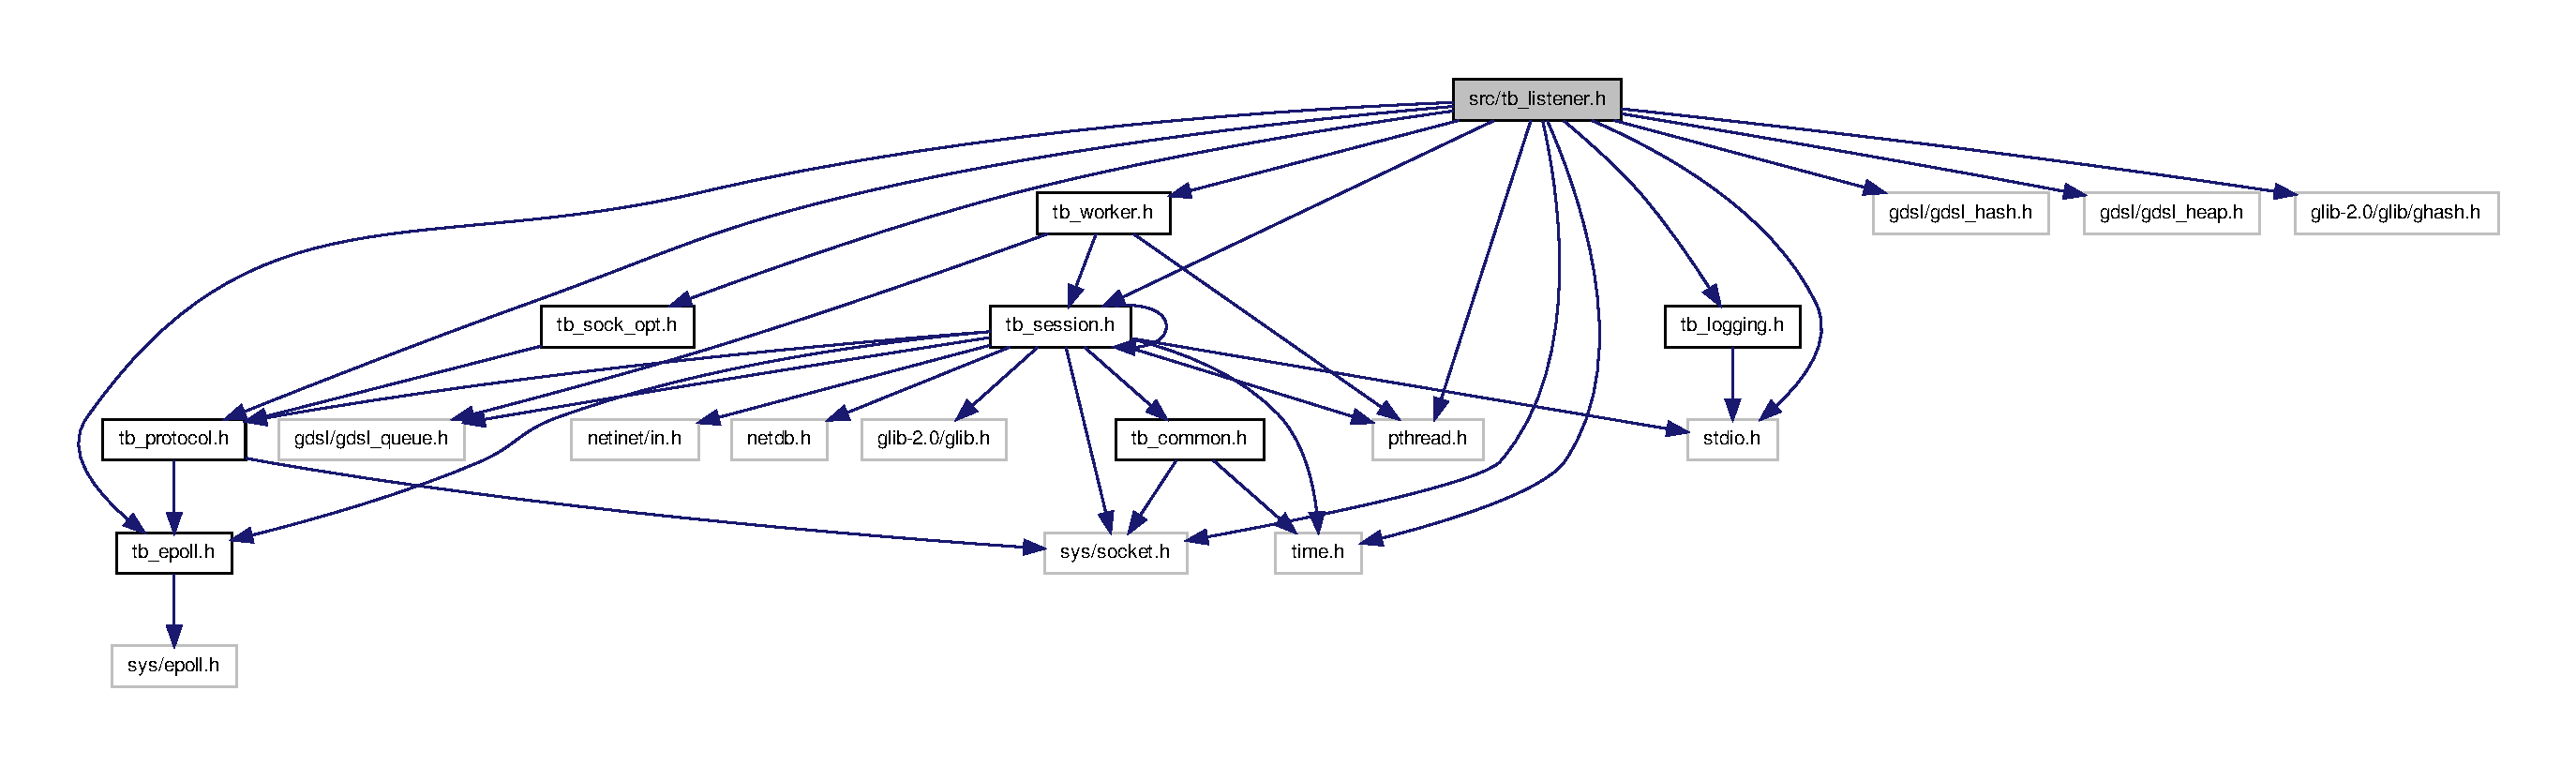
\includegraphics[width=350pt]{tb__listener_8h__incl}
\end{center}
\end{figure}
This graph shows which files directly or indirectly include this file\-:\nopagebreak
\begin{figure}[H]
\begin{center}
\leavevmode
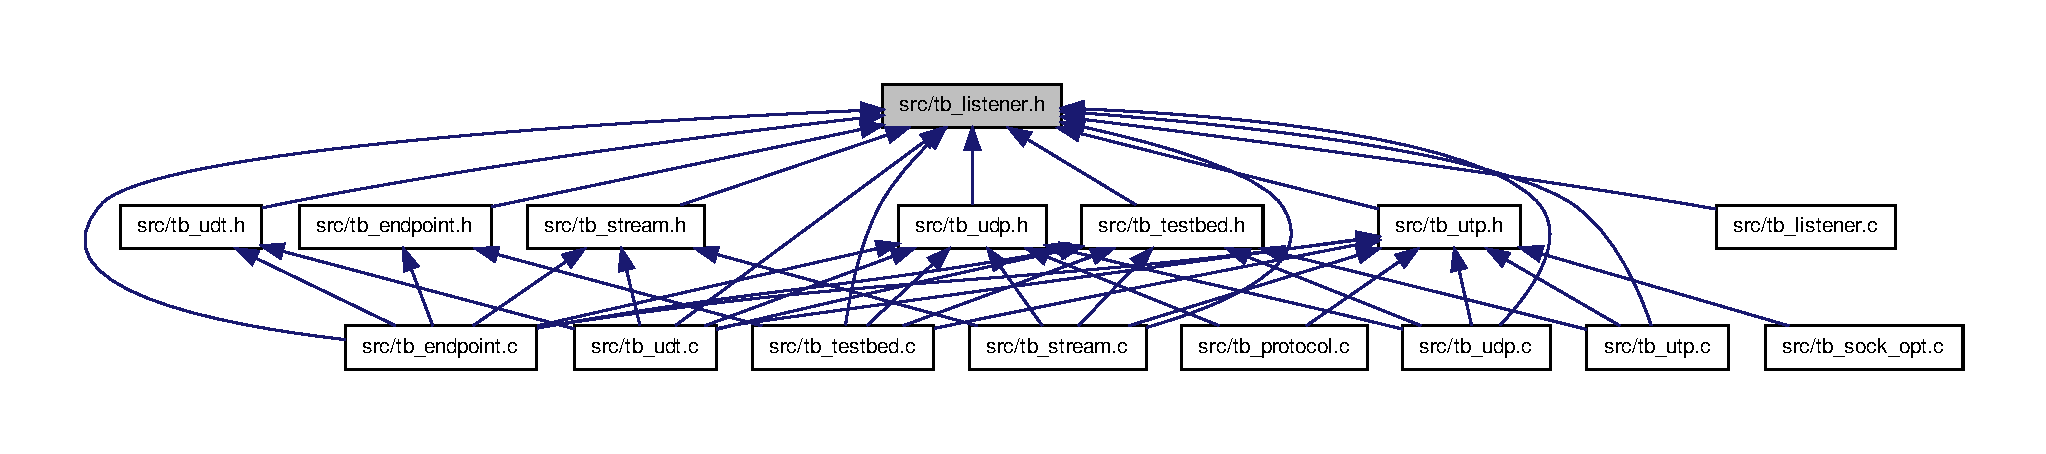
\includegraphics[width=350pt]{tb__listener_8h__dep__incl}
\end{center}
\end{figure}
\subsection*{Data Structures}
\begin{DoxyCompactItemize}
\item 
struct \hyperlink{structtb__test__params__t}{tb\-\_\-test\-\_\-params\-\_\-t}
\item 
struct \hyperlink{structtb__listener__t}{tb\-\_\-listener\-\_\-t}
\item 
struct \hyperlink{structtb__other__info}{tb\-\_\-other\-\_\-info}
\end{DoxyCompactItemize}
\subsection*{Typedefs}
\begin{DoxyCompactItemize}
\item 
typedef void($\ast$ \hyperlink{tb__listener_8h_a087aa7eae6394f6a052ea86a8944b262}{funct\-\_\-l\-\_\-exit} )(void $\ast$listener)
\item 
typedef void($\ast$ \hyperlink{tb__listener_8h_a26990e2906e18234aa32e757383e1752}{funct\-\_\-l\-\_\-abort} )(void $\ast$listener)
\end{DoxyCompactItemize}
\subsection*{Enumerations}
\begin{DoxyCompactItemize}
\item 
enum \hyperlink{tb__listener_8h_ae37f3ebcf0081b2dd11adf41f1f867d6}{E\-N\-D\-P\-O\-I\-N\-T\-\_\-\-T\-Y\-P\-E} \{ \hyperlink{tb__listener_8h_ae37f3ebcf0081b2dd11adf41f1f867d6a67c96b24b23bcb408bae7626730a04b7}{S\-E\-R\-V\-E\-R} =  0, 
\hyperlink{tb__listener_8h_ae37f3ebcf0081b2dd11adf41f1f867d6a48e4cb37544c8e69715d45e5a83b2109}{C\-L\-I\-E\-N\-T}, 
\hyperlink{tb__listener_8h_ae37f3ebcf0081b2dd11adf41f1f867d6a279284d2b9d6f1a10042b926951b77ab}{m\-S\-E\-R\-V\-E\-R}, 
\hyperlink{tb__listener_8h_ae37f3ebcf0081b2dd11adf41f1f867d6aee914d963bee5cbcdec16ea2d5432d75}{m\-C\-L\-I\-E\-N\-T}
 \}
\item 
enum \hyperlink{tb__listener_8h_a32c27cc471df37f4fc818d65de0a56c4}{S\-T\-A\-T\-U\-S} \{ \\*
\hyperlink{tb__listener_8h_a32c27cc471df37f4fc818d65de0a56c4a7ef9ab2ee648332deb26886b5f5a198e}{T\-B\-\_\-\-C\-R\-E\-A\-T\-E\-D} =  0, 
\hyperlink{tb__listener_8h_a32c27cc471df37f4fc818d65de0a56c4ae3f258303bb903e4a10660a64c2af1ee}{T\-B\-\_\-\-S\-T\-A\-R\-T\-I\-N\-G} =  1, 
\hyperlink{tb__listener_8h_a32c27cc471df37f4fc818d65de0a56c4a85db1220e76bb25e4d4bac5b3c3b524f}{T\-B\-\_\-\-C\-O\-N\-N\-E\-C\-T\-E\-D} =  2, 
\hyperlink{tb__listener_8h_a32c27cc471df37f4fc818d65de0a56c4ad4e334774bf8113c5f695116c31e4fc0}{T\-B\-\_\-\-D\-I\-S\-C\-O\-N\-N\-E\-C\-T\-E\-D} =  3, 
\\*
\hyperlink{tb__listener_8h_a32c27cc471df37f4fc818d65de0a56c4a0431dc834b1dedce4f5694b274f7d22e}{T\-B\-\_\-\-L\-I\-S\-T\-E\-N\-I\-N\-G} =  4, 
\hyperlink{tb__listener_8h_a32c27cc471df37f4fc818d65de0a56c4a2a7704cb5e60a9f197267978817c7007}{T\-B\-\_\-\-E\-X\-I\-T\-I\-N\-G} =  5, 
\hyperlink{tb__listener_8h_a32c27cc471df37f4fc818d65de0a56c4aa5e00e821cf2b9ce1dd4286178970058}{T\-B\-\_\-\-A\-B\-O\-R\-T\-I\-N\-G} =  6, 
\hyperlink{tb__listener_8h_a32c27cc471df37f4fc818d65de0a56c4a5d8f10dd221cadd7fdabb80df931d575}{T\-B\-\_\-\-P\-O\-L\-L\-I\-N\-G} =  7
 \}
\item 
enum \hyperlink{tb__listener_8h_a0fbada5bff0eeb4dc6be4b6e6f1c4eaf}{C\-O\-M\-M\-A\-N\-D} \{ \hyperlink{tb__listener_8h_a0fbada5bff0eeb4dc6be4b6e6f1c4eafa13e252fc01cca534ed6aa612e99f2173}{T\-B\-\_\-\-C\-O\-N\-T\-I\-N\-U\-E} =  1, 
\hyperlink{tb__listener_8h_a0fbada5bff0eeb4dc6be4b6e6f1c4eafaf76138418fd9d2bb1c239fc8c68a8774}{T\-B\-\_\-\-A\-B\-O\-R\-T} =  2, 
\hyperlink{tb__listener_8h_a0fbada5bff0eeb4dc6be4b6e6f1c4eafa96efcde6db8a86a5aea96d8a5963a7c4}{T\-B\-\_\-\-E\-X\-I\-T} =  4, 
\hyperlink{tb__listener_8h_a0fbada5bff0eeb4dc6be4b6e6f1c4eafa931ee640196d62acef98f47b54b20a4d}{T\-B\-\_\-\-E\-\_\-\-L\-O\-O\-P} =  T\-B\-\_\-\-A\-B\-O\-R\-T $|$ T\-B\-\_\-\-E\-X\-I\-T
 \}
\end{DoxyCompactItemize}
\subsection*{Functions}
\begin{DoxyCompactItemize}
\item 
void \hyperlink{tb__listener_8h_ae063a1fdce497a4e08aea504a6ab927b}{tb\-\_\-set\-\_\-l\-\_\-stats} (\hyperlink{structtb__listener__t}{tb\-\_\-listener\-\_\-t} $\ast$listener)
\begin{DoxyCompactList}\small\item\em Gets the stats for the listener. \end{DoxyCompactList}\item 
void \hyperlink{tb__listener_8h_a144e59e2470a90fc2b6e1f840da77ae8}{tb\-\_\-set\-\_\-m\-\_\-stats} (\hyperlink{structtb__listener__t}{tb\-\_\-listener\-\_\-t} $\ast$listener)
\begin{DoxyCompactList}\small\item\em Gets the stats for the listener. \end{DoxyCompactList}\item 
\hyperlink{structtb__prot__stats__t}{tb\-\_\-prot\-\_\-stats\-\_\-t} $\ast$ \hyperlink{tb__listener_8h_a6e5c88a915882ea9d39fd41ee4742ffc}{tb\-\_\-ex\-\_\-get\-\_\-stats} (\hyperlink{structtb__listener__t}{tb\-\_\-listener\-\_\-t} $\ast$listener)
\begin{DoxyCompactList}\small\item\em A thread safe way to get access to stats. \end{DoxyCompactList}\item 
\hyperlink{structtb__listener__t}{tb\-\_\-listener\-\_\-t} $\ast$ \hyperlink{tb__listener_8h_a5ec3b6c120621050965582e51e4d0d5a}{tb\-\_\-create\-\_\-listener} (\hyperlink{tb__listener_8h_ae37f3ebcf0081b2dd11adf41f1f867d6}{E\-N\-D\-P\-O\-I\-N\-T\-\_\-\-T\-Y\-P\-E} type, char $\ast$addr, char $\ast$port, \hyperlink{tb__protocol_8h_a7a5bff1040fc154c510874327d44cc1a}{P\-R\-O\-T\-O\-C\-O\-L} protocol, int bufsize)
\begin{DoxyCompactList}\small\item\em Create a listener with the supplied parameters. \end{DoxyCompactList}\item 
\hyperlink{structtb__listener__t}{tb\-\_\-listener\-\_\-t} $\ast$ \hyperlink{tb__listener_8h_a042a2b565ccc70e1506562ad43c83bfb}{tb\-\_\-create\-\_\-endpoint} (\hyperlink{structtb__test__params__t}{tb\-\_\-test\-\_\-params\-\_\-t} $\ast$params)
\begin{DoxyCompactList}\small\item\em Create a listener using a \hyperlink{structtb__test__params__t}{tb\-\_\-test\-\_\-params\-\_\-t} struct. \end{DoxyCompactList}\item 
\hyperlink{structtb__worker__t}{tb\-\_\-worker\-\_\-t} $\ast$ \hyperlink{tb__listener_8h_aadc6c1af686cf9fc7bbd8874eca3be42}{tb\-\_\-get\-\_\-worker} (\hyperlink{structtb__listener__t}{tb\-\_\-listener\-\_\-t} $\ast$listener, \hyperlink{structtb__session__t}{tb\-\_\-session\-\_\-t} $\ast$session)
\begin{DoxyCompactList}\small\item\em Get a worker for the supplied session. \end{DoxyCompactList}\item 
void \hyperlink{tb__listener_8h_a370d0eb443de6db87ab002ea2e5cc468}{tb\-\_\-destroy\-\_\-listener} (\hyperlink{structtb__listener__t}{tb\-\_\-listener\-\_\-t} $\ast$listener)
\begin{DoxyCompactList}\small\item\em Destroy a listener. \end{DoxyCompactList}\item 
int \hyperlink{tb__listener_8h_a3ef8c04e8f0f2aed65b59821d3a1b01d}{tb\-\_\-set\-\_\-therad\-\_\-param} (\hyperlink{structtb__listener__t}{tb\-\_\-listener\-\_\-t} $\ast$listener)
\begin{DoxyCompactList}\small\item\em Set the affinity and scheduling priority for a given thread. \end{DoxyCompactList}\item 
void \hyperlink{tb__listener_8h_aa1646d6df4318c903d2653a6032a0a40}{tb\-\_\-get\-\_\-cpu\-\_\-info} (\hyperlink{structtb__listener__t}{tb\-\_\-listener\-\_\-t} $\ast$listener)
\item 
void \hyperlink{tb__listener_8h_af552255cac39c1b712a1c213070c04e0}{tb\-\_\-print\-\_\-listener} (\hyperlink{structtb__listener__t}{tb\-\_\-listener\-\_\-t} $\ast$listener)
\begin{DoxyCompactList}\small\item\em Print a listener. \end{DoxyCompactList}\item 
int \hyperlink{tb__listener_8h_aedd19f27c5b2e1d8717024afed30ec51}{tb\-\_\-resolve\-\_\-address} (\hyperlink{structtb__listener__t}{tb\-\_\-listener\-\_\-t} $\ast$listener)
\begin{DoxyCompactList}\small\item\em Resolve the address for the given listener. \end{DoxyCompactList}\item 
int \hyperlink{tb__listener_8h_a15dfa6415134b86b0a24bb01eece50ee}{tb\-\_\-set\-\_\-sockopt} (\hyperlink{structtb__listener__t}{tb\-\_\-listener\-\_\-t} $\ast$listener)
\begin{DoxyCompactList}\small\item\em Set sockopt. \end{DoxyCompactList}\item 
int \hyperlink{tb__listener_8h_ac2e55c5098e2f7105812f5947860cf45}{tb\-\_\-create\-\_\-socket} (\hyperlink{structtb__listener__t}{tb\-\_\-listener\-\_\-t} $\ast$listener) \-\_\-\-\_\-attribute\-\_\-\-\_\-((always\-\_\-inline))
\begin{DoxyCompactList}\small\item\em Create a socket. \end{DoxyCompactList}\item 
int \hyperlink{tb__listener_8h_a818e46957ec1b6d9498b03c42d3e962a}{tb\-\_\-listen} (\hyperlink{structtb__listener__t}{tb\-\_\-listener\-\_\-t} $\ast$listener) \-\_\-\-\_\-attribute\-\_\-\-\_\-((always\-\_\-inline))
\begin{DoxyCompactList}\small\item\em Bind and listen. \end{DoxyCompactList}\item 
\hyperlink{structtb__session__t}{tb\-\_\-session\-\_\-t} $\ast$ \hyperlink{tb__listener_8h_a4fc2236ebc38eb60b93471a9e5162d92}{tb\-\_\-accept} (\hyperlink{structtb__listener__t}{tb\-\_\-listener\-\_\-t} $\ast$listener) \-\_\-\-\_\-attribute\-\_\-\-\_\-((always\-\_\-inline))
\begin{DoxyCompactList}\small\item\em Accept an incoming connection. \end{DoxyCompactList}\item 
int \hyperlink{tb__listener_8h_ab13164809a5b7d6ce88a2e3156096f8c}{tb\-\_\-connect} (\hyperlink{structtb__listener__t}{tb\-\_\-listener\-\_\-t} $\ast$listener) \-\_\-\-\_\-attribute\-\_\-\-\_\-((always\-\_\-inline))
\begin{DoxyCompactList}\small\item\em Attempt to connect. \end{DoxyCompactList}\item 
int \hyperlink{tb__listener_8h_ae886708c5c2a62a435422948143d6e69}{tb\-\_\-bind} (\hyperlink{structtb__listener__t}{tb\-\_\-listener\-\_\-t} $\ast$listener) \-\_\-\-\_\-attribute\-\_\-\-\_\-((always\-\_\-inline))
\begin{DoxyCompactList}\small\item\em Bind the listener to its address. \end{DoxyCompactList}\item 
int \hyperlink{tb__listener_8h_a9801fb8797f4a9bab6e99be129ff3304}{tb\-\_\-send\-\_\-data} (\hyperlink{structtb__listener__t}{tb\-\_\-listener\-\_\-t} $\ast$listener, char $\ast$buff, int size) \-\_\-\-\_\-attribute\-\_\-\-\_\-((always\-\_\-inline))
\begin{DoxyCompactList}\small\item\em Send data. \end{DoxyCompactList}\item 
int \hyperlink{tb__listener_8h_ae2ea1c34daca7877a7acae3afa17427f}{tb\-\_\-recv\-\_\-data} (\hyperlink{structtb__listener__t}{tb\-\_\-listener\-\_\-t} $\ast$listener, \hyperlink{structtb__session__t}{tb\-\_\-session\-\_\-t} $\ast$session) \-\_\-\-\_\-attribute\-\_\-\-\_\-((always\-\_\-inline))
\begin{DoxyCompactList}\small\item\em Receive data. \end{DoxyCompactList}\item 
int \hyperlink{tb__listener_8h_ae70c851b28d81589f2648ce018e727bd}{tb\-\_\-send\-\_\-to} (\hyperlink{structtb__listener__t}{tb\-\_\-listener\-\_\-t} $\ast$listener, \hyperlink{structtb__session__t}{tb\-\_\-session\-\_\-t} $\ast$session) \-\_\-\-\_\-attribute\-\_\-\-\_\-((always\-\_\-inline))
\item 
int \hyperlink{tb__listener_8h_afec61a9f694c57aec84cc5a2d520b001}{tb\-\_\-recv\-\_\-from} (\hyperlink{structtb__listener__t}{tb\-\_\-listener\-\_\-t} $\ast$listener, \hyperlink{structtb__session__t}{tb\-\_\-session\-\_\-t} $\ast$session) \-\_\-\-\_\-attribute\-\_\-\-\_\-((always\-\_\-inline))
\begin{DoxyCompactList}\small\item\em recv from -\/ used by U\-D\-P. \end{DoxyCompactList}\item 
void \hyperlink{tb__listener_8h_ac09710b23dca8fcf1c05f4bd4c707b7a}{tb\-\_\-get\-\_\-prot\-\_\-stats} (\hyperlink{structtb__listener__t}{tb\-\_\-listener\-\_\-t} $\ast$listener)
\begin{DoxyCompactList}\small\item\em collect stats for listener. \end{DoxyCompactList}\item 
int \hyperlink{tb__listener_8h_a633cfdcf57f29c6e1ae09044ed483794}{tb\-\_\-set\-\_\-epoll} (\hyperlink{structtb__listener__t}{tb\-\_\-listener\-\_\-t} $\ast$listener) \-\_\-\-\_\-attribute\-\_\-\-\_\-((always\-\_\-inline))
\begin{DoxyCompactList}\small\item\em Set epoll for this listener. \end{DoxyCompactList}\item 
void \hyperlink{tb__listener_8h_a233900871cf97b4af517dcf4bbdd5d6b}{tb\-\_\-error} (\hyperlink{structtb__listener__t}{tb\-\_\-listener\-\_\-t} $\ast$listener, const char $\ast$info, int errno) \-\_\-\-\_\-attribute\-\_\-\-\_\-((always\-\_\-inline))
\begin{DoxyCompactList}\small\item\em Format an error to the log file. \end{DoxyCompactList}\item 
void \hyperlink{tb__listener_8h_ae35166dd784547cfb9d71a3b9af3dd2b}{tb\-\_\-address} (\hyperlink{structtb__listener__t}{tb\-\_\-listener\-\_\-t} $\ast$listener, const char $\ast$info, struct sockaddr\-\_\-storage $\ast$store) \-\_\-\-\_\-attribute\-\_\-\-\_\-((always\-\_\-inline))
\end{DoxyCompactItemize}


\subsection{Typedef Documentation}
\hypertarget{tb__listener_8h_a26990e2906e18234aa32e757383e1752}{\index{tb\-\_\-listener.\-h@{tb\-\_\-listener.\-h}!funct\-\_\-l\-\_\-abort@{funct\-\_\-l\-\_\-abort}}
\index{funct\-\_\-l\-\_\-abort@{funct\-\_\-l\-\_\-abort}!tb_listener.h@{tb\-\_\-listener.\-h}}
\subsubsection[{funct\-\_\-l\-\_\-abort}]{\setlength{\rightskip}{0pt plus 5cm}typedef void($\ast$ funct\-\_\-l\-\_\-abort)(void $\ast$listener)}}\label{tb__listener_8h_a26990e2906e18234aa32e757383e1752}


Definition at line 125 of file tb\-\_\-listener.\-h.

\hypertarget{tb__listener_8h_a087aa7eae6394f6a052ea86a8944b262}{\index{tb\-\_\-listener.\-h@{tb\-\_\-listener.\-h}!funct\-\_\-l\-\_\-exit@{funct\-\_\-l\-\_\-exit}}
\index{funct\-\_\-l\-\_\-exit@{funct\-\_\-l\-\_\-exit}!tb_listener.h@{tb\-\_\-listener.\-h}}
\subsubsection[{funct\-\_\-l\-\_\-exit}]{\setlength{\rightskip}{0pt plus 5cm}typedef void($\ast$ funct\-\_\-l\-\_\-exit)(void $\ast$listener)}}\label{tb__listener_8h_a087aa7eae6394f6a052ea86a8944b262}


Definition at line 119 of file tb\-\_\-listener.\-h.



\subsection{Enumeration Type Documentation}
\hypertarget{tb__listener_8h_a0fbada5bff0eeb4dc6be4b6e6f1c4eaf}{\index{tb\-\_\-listener.\-h@{tb\-\_\-listener.\-h}!C\-O\-M\-M\-A\-N\-D@{C\-O\-M\-M\-A\-N\-D}}
\index{C\-O\-M\-M\-A\-N\-D@{C\-O\-M\-M\-A\-N\-D}!tb_listener.h@{tb\-\_\-listener.\-h}}
\subsubsection[{C\-O\-M\-M\-A\-N\-D}]{\setlength{\rightskip}{0pt plus 5cm}enum {\bf C\-O\-M\-M\-A\-N\-D}}}\label{tb__listener_8h_a0fbada5bff0eeb4dc6be4b6e6f1c4eaf}
\begin{Desc}
\item[Enumerator\-: ]\par
\begin{description}
\index{T\-B\-\_\-\-C\-O\-N\-T\-I\-N\-U\-E@{T\-B\-\_\-\-C\-O\-N\-T\-I\-N\-U\-E}!tb\-\_\-listener.\-h@{tb\-\_\-listener.\-h}}\index{tb\-\_\-listener.\-h@{tb\-\_\-listener.\-h}!T\-B\-\_\-\-C\-O\-N\-T\-I\-N\-U\-E@{T\-B\-\_\-\-C\-O\-N\-T\-I\-N\-U\-E}}\item[{\em 
\hypertarget{tb__listener_8h_a0fbada5bff0eeb4dc6be4b6e6f1c4eafa13e252fc01cca534ed6aa612e99f2173}{T\-B\-\_\-\-C\-O\-N\-T\-I\-N\-U\-E}\label{tb__listener_8h_a0fbada5bff0eeb4dc6be4b6e6f1c4eafa13e252fc01cca534ed6aa612e99f2173}
}]Regular status. \index{T\-B\-\_\-\-A\-B\-O\-R\-T@{T\-B\-\_\-\-A\-B\-O\-R\-T}!tb\-\_\-listener.\-h@{tb\-\_\-listener.\-h}}\index{tb\-\_\-listener.\-h@{tb\-\_\-listener.\-h}!T\-B\-\_\-\-A\-B\-O\-R\-T@{T\-B\-\_\-\-A\-B\-O\-R\-T}}\item[{\em 
\hypertarget{tb__listener_8h_a0fbada5bff0eeb4dc6be4b6e6f1c4eafaf76138418fd9d2bb1c239fc8c68a8774}{T\-B\-\_\-\-A\-B\-O\-R\-T}\label{tb__listener_8h_a0fbada5bff0eeb4dc6be4b6e6f1c4eafaf76138418fd9d2bb1c239fc8c68a8774}
}]Abort the current operation. \index{T\-B\-\_\-\-E\-X\-I\-T@{T\-B\-\_\-\-E\-X\-I\-T}!tb\-\_\-listener.\-h@{tb\-\_\-listener.\-h}}\index{tb\-\_\-listener.\-h@{tb\-\_\-listener.\-h}!T\-B\-\_\-\-E\-X\-I\-T@{T\-B\-\_\-\-E\-X\-I\-T}}\item[{\em 
\hypertarget{tb__listener_8h_a0fbada5bff0eeb4dc6be4b6e6f1c4eafa96efcde6db8a86a5aea96d8a5963a7c4}{T\-B\-\_\-\-E\-X\-I\-T}\label{tb__listener_8h_a0fbada5bff0eeb4dc6be4b6e6f1c4eafa96efcde6db8a86a5aea96d8a5963a7c4}
}]Exit from the current operation. \index{T\-B\-\_\-\-E\-\_\-\-L\-O\-O\-P@{T\-B\-\_\-\-E\-\_\-\-L\-O\-O\-P}!tb\-\_\-listener.\-h@{tb\-\_\-listener.\-h}}\index{tb\-\_\-listener.\-h@{tb\-\_\-listener.\-h}!T\-B\-\_\-\-E\-\_\-\-L\-O\-O\-P@{T\-B\-\_\-\-E\-\_\-\-L\-O\-O\-P}}\item[{\em 
\hypertarget{tb__listener_8h_a0fbada5bff0eeb4dc6be4b6e6f1c4eafa931ee640196d62acef98f47b54b20a4d}{T\-B\-\_\-\-E\-\_\-\-L\-O\-O\-P}\label{tb__listener_8h_a0fbada5bff0eeb4dc6be4b6e6f1c4eafa931ee640196d62acef98f47b54b20a4d}
}]Exit from loop. \end{description}
\end{Desc}



Definition at line 64 of file tb\-\_\-listener.\-h.

\hypertarget{tb__listener_8h_ae37f3ebcf0081b2dd11adf41f1f867d6}{\index{tb\-\_\-listener.\-h@{tb\-\_\-listener.\-h}!E\-N\-D\-P\-O\-I\-N\-T\-\_\-\-T\-Y\-P\-E@{E\-N\-D\-P\-O\-I\-N\-T\-\_\-\-T\-Y\-P\-E}}
\index{E\-N\-D\-P\-O\-I\-N\-T\-\_\-\-T\-Y\-P\-E@{E\-N\-D\-P\-O\-I\-N\-T\-\_\-\-T\-Y\-P\-E}!tb_listener.h@{tb\-\_\-listener.\-h}}
\subsubsection[{E\-N\-D\-P\-O\-I\-N\-T\-\_\-\-T\-Y\-P\-E}]{\setlength{\rightskip}{0pt plus 5cm}enum {\bf E\-N\-D\-P\-O\-I\-N\-T\-\_\-\-T\-Y\-P\-E}}}\label{tb__listener_8h_ae37f3ebcf0081b2dd11adf41f1f867d6}
\begin{Desc}
\item[Enumerator\-: ]\par
\begin{description}
\index{S\-E\-R\-V\-E\-R@{S\-E\-R\-V\-E\-R}!tb\-\_\-listener.\-h@{tb\-\_\-listener.\-h}}\index{tb\-\_\-listener.\-h@{tb\-\_\-listener.\-h}!S\-E\-R\-V\-E\-R@{S\-E\-R\-V\-E\-R}}\item[{\em 
\hypertarget{tb__listener_8h_ae37f3ebcf0081b2dd11adf41f1f867d6a67c96b24b23bcb408bae7626730a04b7}{S\-E\-R\-V\-E\-R}\label{tb__listener_8h_ae37f3ebcf0081b2dd11adf41f1f867d6a67c96b24b23bcb408bae7626730a04b7}
}]The listener is a server. \index{C\-L\-I\-E\-N\-T@{C\-L\-I\-E\-N\-T}!tb\-\_\-listener.\-h@{tb\-\_\-listener.\-h}}\index{tb\-\_\-listener.\-h@{tb\-\_\-listener.\-h}!C\-L\-I\-E\-N\-T@{C\-L\-I\-E\-N\-T}}\item[{\em 
\hypertarget{tb__listener_8h_ae37f3ebcf0081b2dd11adf41f1f867d6a48e4cb37544c8e69715d45e5a83b2109}{C\-L\-I\-E\-N\-T}\label{tb__listener_8h_ae37f3ebcf0081b2dd11adf41f1f867d6a48e4cb37544c8e69715d45e5a83b2109}
}]The listener is a client. \index{m\-S\-E\-R\-V\-E\-R@{m\-S\-E\-R\-V\-E\-R}!tb\-\_\-listener.\-h@{tb\-\_\-listener.\-h}}\index{tb\-\_\-listener.\-h@{tb\-\_\-listener.\-h}!m\-S\-E\-R\-V\-E\-R@{m\-S\-E\-R\-V\-E\-R}}\item[{\em 
\hypertarget{tb__listener_8h_ae37f3ebcf0081b2dd11adf41f1f867d6a279284d2b9d6f1a10042b926951b77ab}{m\-S\-E\-R\-V\-E\-R}\label{tb__listener_8h_ae37f3ebcf0081b2dd11adf41f1f867d6a279284d2b9d6f1a10042b926951b77ab}
}]Multi connection server. \index{m\-C\-L\-I\-E\-N\-T@{m\-C\-L\-I\-E\-N\-T}!tb\-\_\-listener.\-h@{tb\-\_\-listener.\-h}}\index{tb\-\_\-listener.\-h@{tb\-\_\-listener.\-h}!m\-C\-L\-I\-E\-N\-T@{m\-C\-L\-I\-E\-N\-T}}\item[{\em 
\hypertarget{tb__listener_8h_ae37f3ebcf0081b2dd11adf41f1f867d6aee914d963bee5cbcdec16ea2d5432d75}{m\-C\-L\-I\-E\-N\-T}\label{tb__listener_8h_ae37f3ebcf0081b2dd11adf41f1f867d6aee914d963bee5cbcdec16ea2d5432d75}
}]Multi connection client. \end{description}
\end{Desc}



Definition at line 32 of file tb\-\_\-listener.\-h.

\hypertarget{tb__listener_8h_a32c27cc471df37f4fc818d65de0a56c4}{\index{tb\-\_\-listener.\-h@{tb\-\_\-listener.\-h}!S\-T\-A\-T\-U\-S@{S\-T\-A\-T\-U\-S}}
\index{S\-T\-A\-T\-U\-S@{S\-T\-A\-T\-U\-S}!tb_listener.h@{tb\-\_\-listener.\-h}}
\subsubsection[{S\-T\-A\-T\-U\-S}]{\setlength{\rightskip}{0pt plus 5cm}enum {\bf S\-T\-A\-T\-U\-S}}}\label{tb__listener_8h_a32c27cc471df37f4fc818d65de0a56c4}
\begin{Desc}
\item[Enumerator\-: ]\par
\begin{description}
\index{T\-B\-\_\-\-C\-R\-E\-A\-T\-E\-D@{T\-B\-\_\-\-C\-R\-E\-A\-T\-E\-D}!tb\-\_\-listener.\-h@{tb\-\_\-listener.\-h}}\index{tb\-\_\-listener.\-h@{tb\-\_\-listener.\-h}!T\-B\-\_\-\-C\-R\-E\-A\-T\-E\-D@{T\-B\-\_\-\-C\-R\-E\-A\-T\-E\-D}}\item[{\em 
\hypertarget{tb__listener_8h_a32c27cc471df37f4fc818d65de0a56c4a7ef9ab2ee648332deb26886b5f5a198e}{T\-B\-\_\-\-C\-R\-E\-A\-T\-E\-D}\label{tb__listener_8h_a32c27cc471df37f4fc818d65de0a56c4a7ef9ab2ee648332deb26886b5f5a198e}
}]The listener has been created. \index{T\-B\-\_\-\-S\-T\-A\-R\-T\-I\-N\-G@{T\-B\-\_\-\-S\-T\-A\-R\-T\-I\-N\-G}!tb\-\_\-listener.\-h@{tb\-\_\-listener.\-h}}\index{tb\-\_\-listener.\-h@{tb\-\_\-listener.\-h}!T\-B\-\_\-\-S\-T\-A\-R\-T\-I\-N\-G@{T\-B\-\_\-\-S\-T\-A\-R\-T\-I\-N\-G}}\item[{\em 
\hypertarget{tb__listener_8h_a32c27cc471df37f4fc818d65de0a56c4ae3f258303bb903e4a10660a64c2af1ee}{T\-B\-\_\-\-S\-T\-A\-R\-T\-I\-N\-G}\label{tb__listener_8h_a32c27cc471df37f4fc818d65de0a56c4ae3f258303bb903e4a10660a64c2af1ee}
}]The listener is starting up. \index{T\-B\-\_\-\-C\-O\-N\-N\-E\-C\-T\-E\-D@{T\-B\-\_\-\-C\-O\-N\-N\-E\-C\-T\-E\-D}!tb\-\_\-listener.\-h@{tb\-\_\-listener.\-h}}\index{tb\-\_\-listener.\-h@{tb\-\_\-listener.\-h}!T\-B\-\_\-\-C\-O\-N\-N\-E\-C\-T\-E\-D@{T\-B\-\_\-\-C\-O\-N\-N\-E\-C\-T\-E\-D}}\item[{\em 
\hypertarget{tb__listener_8h_a32c27cc471df37f4fc818d65de0a56c4a85db1220e76bb25e4d4bac5b3c3b524f}{T\-B\-\_\-\-C\-O\-N\-N\-E\-C\-T\-E\-D}\label{tb__listener_8h_a32c27cc471df37f4fc818d65de0a56c4a85db1220e76bb25e4d4bac5b3c3b524f}
}]The listener is connected. \index{T\-B\-\_\-\-D\-I\-S\-C\-O\-N\-N\-E\-C\-T\-E\-D@{T\-B\-\_\-\-D\-I\-S\-C\-O\-N\-N\-E\-C\-T\-E\-D}!tb\-\_\-listener.\-h@{tb\-\_\-listener.\-h}}\index{tb\-\_\-listener.\-h@{tb\-\_\-listener.\-h}!T\-B\-\_\-\-D\-I\-S\-C\-O\-N\-N\-E\-C\-T\-E\-D@{T\-B\-\_\-\-D\-I\-S\-C\-O\-N\-N\-E\-C\-T\-E\-D}}\item[{\em 
\hypertarget{tb__listener_8h_a32c27cc471df37f4fc818d65de0a56c4ad4e334774bf8113c5f695116c31e4fc0}{T\-B\-\_\-\-D\-I\-S\-C\-O\-N\-N\-E\-C\-T\-E\-D}\label{tb__listener_8h_a32c27cc471df37f4fc818d65de0a56c4ad4e334774bf8113c5f695116c31e4fc0}
}]The listener is disconnected. \index{T\-B\-\_\-\-L\-I\-S\-T\-E\-N\-I\-N\-G@{T\-B\-\_\-\-L\-I\-S\-T\-E\-N\-I\-N\-G}!tb\-\_\-listener.\-h@{tb\-\_\-listener.\-h}}\index{tb\-\_\-listener.\-h@{tb\-\_\-listener.\-h}!T\-B\-\_\-\-L\-I\-S\-T\-E\-N\-I\-N\-G@{T\-B\-\_\-\-L\-I\-S\-T\-E\-N\-I\-N\-G}}\item[{\em 
\hypertarget{tb__listener_8h_a32c27cc471df37f4fc818d65de0a56c4a0431dc834b1dedce4f5694b274f7d22e}{T\-B\-\_\-\-L\-I\-S\-T\-E\-N\-I\-N\-G}\label{tb__listener_8h_a32c27cc471df37f4fc818d65de0a56c4a0431dc834b1dedce4f5694b274f7d22e}
}]The listener is listening for incoming connections. \index{T\-B\-\_\-\-E\-X\-I\-T\-I\-N\-G@{T\-B\-\_\-\-E\-X\-I\-T\-I\-N\-G}!tb\-\_\-listener.\-h@{tb\-\_\-listener.\-h}}\index{tb\-\_\-listener.\-h@{tb\-\_\-listener.\-h}!T\-B\-\_\-\-E\-X\-I\-T\-I\-N\-G@{T\-B\-\_\-\-E\-X\-I\-T\-I\-N\-G}}\item[{\em 
\hypertarget{tb__listener_8h_a32c27cc471df37f4fc818d65de0a56c4a2a7704cb5e60a9f197267978817c7007}{T\-B\-\_\-\-E\-X\-I\-T\-I\-N\-G}\label{tb__listener_8h_a32c27cc471df37f4fc818d65de0a56c4a2a7704cb5e60a9f197267978817c7007}
}]The listener is exiting. \index{T\-B\-\_\-\-A\-B\-O\-R\-T\-I\-N\-G@{T\-B\-\_\-\-A\-B\-O\-R\-T\-I\-N\-G}!tb\-\_\-listener.\-h@{tb\-\_\-listener.\-h}}\index{tb\-\_\-listener.\-h@{tb\-\_\-listener.\-h}!T\-B\-\_\-\-A\-B\-O\-R\-T\-I\-N\-G@{T\-B\-\_\-\-A\-B\-O\-R\-T\-I\-N\-G}}\item[{\em 
\hypertarget{tb__listener_8h_a32c27cc471df37f4fc818d65de0a56c4aa5e00e821cf2b9ce1dd4286178970058}{T\-B\-\_\-\-A\-B\-O\-R\-T\-I\-N\-G}\label{tb__listener_8h_a32c27cc471df37f4fc818d65de0a56c4aa5e00e821cf2b9ce1dd4286178970058}
}]The listener is aborting. \index{T\-B\-\_\-\-P\-O\-L\-L\-I\-N\-G@{T\-B\-\_\-\-P\-O\-L\-L\-I\-N\-G}!tb\-\_\-listener.\-h@{tb\-\_\-listener.\-h}}\index{tb\-\_\-listener.\-h@{tb\-\_\-listener.\-h}!T\-B\-\_\-\-P\-O\-L\-L\-I\-N\-G@{T\-B\-\_\-\-P\-O\-L\-L\-I\-N\-G}}\item[{\em 
\hypertarget{tb__listener_8h_a32c27cc471df37f4fc818d65de0a56c4a5d8f10dd221cadd7fdabb80df931d575}{T\-B\-\_\-\-P\-O\-L\-L\-I\-N\-G}\label{tb__listener_8h_a32c27cc471df37f4fc818d65de0a56c4a5d8f10dd221cadd7fdabb80df931d575}
}]The listener is polling. \end{description}
\end{Desc}



Definition at line 46 of file tb\-\_\-listener.\-h.



\subsection{Function Documentation}
\hypertarget{tb__listener_8h_a4fc2236ebc38eb60b93471a9e5162d92}{\index{tb\-\_\-listener.\-h@{tb\-\_\-listener.\-h}!tb\-\_\-accept@{tb\-\_\-accept}}
\index{tb\-\_\-accept@{tb\-\_\-accept}!tb_listener.h@{tb\-\_\-listener.\-h}}
\subsubsection[{tb\-\_\-accept}]{\setlength{\rightskip}{0pt plus 5cm}{\bf tb\-\_\-session\-\_\-t}$\ast$ tb\-\_\-accept (
\begin{DoxyParamCaption}
\item[{{\bf tb\-\_\-listener\-\_\-t} $\ast$}]{listener}
\end{DoxyParamCaption}
)\hspace{0.3cm}{\ttfamily [inline]}}}\label{tb__listener_8h_a4fc2236ebc38eb60b93471a9e5162d92}


Accept an incoming connection. 

Accepts incoming connections. This operation blocks, as we are using blocking I/\-O currently


\begin{DoxyParams}{Parameters}
{\em listener} & The listener to accept the connection on. \\
\hline
\end{DoxyParams}
\begin{DoxyReturn}{Returns}
\hyperlink{structtb__session__t}{tb\-\_\-session\-\_\-t} A newly created session. 
\end{DoxyReturn}


Definition at line 466 of file tb\-\_\-listener.\-c.

\hypertarget{tb__listener_8h_ae35166dd784547cfb9d71a3b9af3dd2b}{\index{tb\-\_\-listener.\-h@{tb\-\_\-listener.\-h}!tb\-\_\-address@{tb\-\_\-address}}
\index{tb\-\_\-address@{tb\-\_\-address}!tb_listener.h@{tb\-\_\-listener.\-h}}
\subsubsection[{tb\-\_\-address}]{\setlength{\rightskip}{0pt plus 5cm}void tb\-\_\-address (
\begin{DoxyParamCaption}
\item[{{\bf tb\-\_\-listener\-\_\-t} $\ast$}]{listener, }
\item[{const char $\ast$}]{info, }
\item[{struct sockaddr\-\_\-storage $\ast$}]{store}
\end{DoxyParamCaption}
)\hspace{0.3cm}{\ttfamily [inline]}}}\label{tb__listener_8h_ae35166dd784547cfb9d71a3b9af3dd2b}


Definition at line 692 of file tb\-\_\-listener.\-c.

\hypertarget{tb__listener_8h_ae886708c5c2a62a435422948143d6e69}{\index{tb\-\_\-listener.\-h@{tb\-\_\-listener.\-h}!tb\-\_\-bind@{tb\-\_\-bind}}
\index{tb\-\_\-bind@{tb\-\_\-bind}!tb_listener.h@{tb\-\_\-listener.\-h}}
\subsubsection[{tb\-\_\-bind}]{\setlength{\rightskip}{0pt plus 5cm}int tb\-\_\-bind (
\begin{DoxyParamCaption}
\item[{{\bf tb\-\_\-listener\-\_\-t} $\ast$}]{listener}
\end{DoxyParamCaption}
)\hspace{0.3cm}{\ttfamily [inline]}}}\label{tb__listener_8h_ae886708c5c2a62a435422948143d6e69}


Bind the listener to its address. 

Binds the listener to the address specified by address.


\begin{DoxyParams}{Parameters}
{\em listener} & The listener to bind. \\
\hline
\end{DoxyParams}
\begin{DoxyReturn}{Returns}
0 on success, -\/1 on failure. 
\end{DoxyReturn}


Definition at line 564 of file tb\-\_\-listener.\-c.

\hypertarget{tb__listener_8h_ab13164809a5b7d6ce88a2e3156096f8c}{\index{tb\-\_\-listener.\-h@{tb\-\_\-listener.\-h}!tb\-\_\-connect@{tb\-\_\-connect}}
\index{tb\-\_\-connect@{tb\-\_\-connect}!tb_listener.h@{tb\-\_\-listener.\-h}}
\subsubsection[{tb\-\_\-connect}]{\setlength{\rightskip}{0pt plus 5cm}int tb\-\_\-connect (
\begin{DoxyParamCaption}
\item[{{\bf tb\-\_\-listener\-\_\-t} $\ast$}]{listener}
\end{DoxyParamCaption}
)\hspace{0.3cm}{\ttfamily [inline]}}}\label{tb__listener_8h_ab13164809a5b7d6ce88a2e3156096f8c}


Attempt to connect. 

Attempts to connect to the specified address and port. 

Definition at line 545 of file tb\-\_\-listener.\-c.

\hypertarget{tb__listener_8h_a042a2b565ccc70e1506562ad43c83bfb}{\index{tb\-\_\-listener.\-h@{tb\-\_\-listener.\-h}!tb\-\_\-create\-\_\-endpoint@{tb\-\_\-create\-\_\-endpoint}}
\index{tb\-\_\-create\-\_\-endpoint@{tb\-\_\-create\-\_\-endpoint}!tb_listener.h@{tb\-\_\-listener.\-h}}
\subsubsection[{tb\-\_\-create\-\_\-endpoint}]{\setlength{\rightskip}{0pt plus 5cm}{\bf tb\-\_\-listener\-\_\-t}$\ast$ tb\-\_\-create\-\_\-endpoint (
\begin{DoxyParamCaption}
\item[{{\bf tb\-\_\-test\-\_\-params\-\_\-t} $\ast$}]{params}
\end{DoxyParamCaption}
)}}\label{tb__listener_8h_a042a2b565ccc70e1506562ad43c83bfb}


Create a listener using a \hyperlink{structtb__test__params__t}{tb\-\_\-test\-\_\-params\-\_\-t} struct. 

The details in the struct are used to create an endpoint for use in testing.


\begin{DoxyParams}{Parameters}
{\em params} & A struct with all of the required details for a test. \\
\hline
\end{DoxyParams}
\begin{DoxyReturn}{Returns}
the endpoint to test with. 
\end{DoxyReturn}


Definition at line 158 of file tb\-\_\-listener.\-c.

\hypertarget{tb__listener_8h_a5ec3b6c120621050965582e51e4d0d5a}{\index{tb\-\_\-listener.\-h@{tb\-\_\-listener.\-h}!tb\-\_\-create\-\_\-listener@{tb\-\_\-create\-\_\-listener}}
\index{tb\-\_\-create\-\_\-listener@{tb\-\_\-create\-\_\-listener}!tb_listener.h@{tb\-\_\-listener.\-h}}
\subsubsection[{tb\-\_\-create\-\_\-listener}]{\setlength{\rightskip}{0pt plus 5cm}{\bf tb\-\_\-listener\-\_\-t}$\ast$ tb\-\_\-create\-\_\-listener (
\begin{DoxyParamCaption}
\item[{{\bf E\-N\-D\-P\-O\-I\-N\-T\-\_\-\-T\-Y\-P\-E}}]{type, }
\item[{char $\ast$}]{addr, }
\item[{char $\ast$}]{port, }
\item[{{\bf P\-R\-O\-T\-O\-C\-O\-L}}]{protocol, }
\item[{int}]{bufsize}
\end{DoxyParamCaption}
)}}\label{tb__listener_8h_a5ec3b6c120621050965582e51e4d0d5a}


Create a listener with the supplied parameters. 

Creates a listener and the accociated data structures.


\begin{DoxyParams}{Parameters}
{\em type} & The type of endpoint to create. \\
\hline
{\em addr} & The address to bind to. \\
\hline
{\em port} & The port to bind to. \\
\hline
{\em num\-\_\-threads} & The number of worker threads to use.\\
\hline
\end{DoxyParams}
\begin{DoxyReturn}{Returns}
The newly created listener. 
\end{DoxyReturn}


Definition at line 38 of file tb\-\_\-listener.\-c.

\hypertarget{tb__listener_8h_ac2e55c5098e2f7105812f5947860cf45}{\index{tb\-\_\-listener.\-h@{tb\-\_\-listener.\-h}!tb\-\_\-create\-\_\-socket@{tb\-\_\-create\-\_\-socket}}
\index{tb\-\_\-create\-\_\-socket@{tb\-\_\-create\-\_\-socket}!tb_listener.h@{tb\-\_\-listener.\-h}}
\subsubsection[{tb\-\_\-create\-\_\-socket}]{\setlength{\rightskip}{0pt plus 5cm}int tb\-\_\-create\-\_\-socket (
\begin{DoxyParamCaption}
\item[{{\bf tb\-\_\-listener\-\_\-t} $\ast$}]{listener}
\end{DoxyParamCaption}
)\hspace{0.3cm}{\ttfamily [inline]}}}\label{tb__listener_8h_ac2e55c5098e2f7105812f5947860cf45}


Create a socket. 

Creates a new socket for the specified listener.


\begin{DoxyParams}{Parameters}
{\em The} & listener to create the socket for. \\
\hline
\end{DoxyParams}


Definition at line 527 of file tb\-\_\-listener.\-c.

\hypertarget{tb__listener_8h_a370d0eb443de6db87ab002ea2e5cc468}{\index{tb\-\_\-listener.\-h@{tb\-\_\-listener.\-h}!tb\-\_\-destroy\-\_\-listener@{tb\-\_\-destroy\-\_\-listener}}
\index{tb\-\_\-destroy\-\_\-listener@{tb\-\_\-destroy\-\_\-listener}!tb_listener.h@{tb\-\_\-listener.\-h}}
\subsubsection[{tb\-\_\-destroy\-\_\-listener}]{\setlength{\rightskip}{0pt plus 5cm}void tb\-\_\-destroy\-\_\-listener (
\begin{DoxyParamCaption}
\item[{{\bf tb\-\_\-listener\-\_\-t} $\ast$}]{listener}
\end{DoxyParamCaption}
)}}\label{tb__listener_8h_a370d0eb443de6db87ab002ea2e5cc468}


Destroy a listener. 

Destroys the listener, and its associated data structures.


\begin{DoxyParams}{Parameters}
{\em listener} & The listener to destroy. \\
\hline
\end{DoxyParams}


Definition at line 282 of file tb\-\_\-listener.\-c.

\hypertarget{tb__listener_8h_a233900871cf97b4af517dcf4bbdd5d6b}{\index{tb\-\_\-listener.\-h@{tb\-\_\-listener.\-h}!tb\-\_\-error@{tb\-\_\-error}}
\index{tb\-\_\-error@{tb\-\_\-error}!tb_listener.h@{tb\-\_\-listener.\-h}}
\subsubsection[{tb\-\_\-error}]{\setlength{\rightskip}{0pt plus 5cm}void tb\-\_\-error (
\begin{DoxyParamCaption}
\item[{{\bf tb\-\_\-listener\-\_\-t} $\ast$}]{listener, }
\item[{const char $\ast$}]{info, }
\item[{int}]{errno}
\end{DoxyParamCaption}
)\hspace{0.3cm}{\ttfamily [inline]}}}\label{tb__listener_8h_a233900871cf97b4af517dcf4bbdd5d6b}


Format an error to the log file. 



Definition at line 676 of file tb\-\_\-listener.\-c.

\hypertarget{tb__listener_8h_a6e5c88a915882ea9d39fd41ee4742ffc}{\index{tb\-\_\-listener.\-h@{tb\-\_\-listener.\-h}!tb\-\_\-ex\-\_\-get\-\_\-stats@{tb\-\_\-ex\-\_\-get\-\_\-stats}}
\index{tb\-\_\-ex\-\_\-get\-\_\-stats@{tb\-\_\-ex\-\_\-get\-\_\-stats}!tb_listener.h@{tb\-\_\-listener.\-h}}
\subsubsection[{tb\-\_\-ex\-\_\-get\-\_\-stats}]{\setlength{\rightskip}{0pt plus 5cm}{\bf tb\-\_\-prot\-\_\-stats\-\_\-t}$\ast$ tb\-\_\-ex\-\_\-get\-\_\-stats (
\begin{DoxyParamCaption}
\item[{{\bf tb\-\_\-listener\-\_\-t} $\ast$}]{listener}
\end{DoxyParamCaption}
)}}\label{tb__listener_8h_a6e5c88a915882ea9d39fd41ee4742ffc}


A thread safe way to get access to stats. 

This method controls access to the stats generated by testbed. These stats are updated every second, and can be read once. If the data that can be obtained by this function has already been read, it blocks until new data has arrived.


\begin{DoxyParams}{Parameters}
{\em listener} & The listener for which to get the stats from. \\
\hline
\end{DoxyParams}
\begin{DoxyReturn}{Returns}
\hyperlink{structtb__prot__stats__t}{tb\-\_\-prot\-\_\-stats\-\_\-t} with the stats inserted. 
\end{DoxyReturn}


Definition at line 362 of file tb\-\_\-listener.\-c.

\hypertarget{tb__listener_8h_aa1646d6df4318c903d2653a6032a0a40}{\index{tb\-\_\-listener.\-h@{tb\-\_\-listener.\-h}!tb\-\_\-get\-\_\-cpu\-\_\-info@{tb\-\_\-get\-\_\-cpu\-\_\-info}}
\index{tb\-\_\-get\-\_\-cpu\-\_\-info@{tb\-\_\-get\-\_\-cpu\-\_\-info}!tb_listener.h@{tb\-\_\-listener.\-h}}
\subsubsection[{tb\-\_\-get\-\_\-cpu\-\_\-info}]{\setlength{\rightskip}{0pt plus 5cm}void tb\-\_\-get\-\_\-cpu\-\_\-info (
\begin{DoxyParamCaption}
\item[{{\bf tb\-\_\-listener\-\_\-t} $\ast$}]{listener}
\end{DoxyParamCaption}
)}}\label{tb__listener_8h_aa1646d6df4318c903d2653a6032a0a40}
Gets the tid from syscall and pthread\-\_\-self, sets them in the listener. 

Definition at line 276 of file tb\-\_\-listener.\-c.

\hypertarget{tb__listener_8h_ac09710b23dca8fcf1c05f4bd4c707b7a}{\index{tb\-\_\-listener.\-h@{tb\-\_\-listener.\-h}!tb\-\_\-get\-\_\-prot\-\_\-stats@{tb\-\_\-get\-\_\-prot\-\_\-stats}}
\index{tb\-\_\-get\-\_\-prot\-\_\-stats@{tb\-\_\-get\-\_\-prot\-\_\-stats}!tb_listener.h@{tb\-\_\-listener.\-h}}
\subsubsection[{tb\-\_\-get\-\_\-prot\-\_\-stats}]{\setlength{\rightskip}{0pt plus 5cm}void tb\-\_\-get\-\_\-prot\-\_\-stats (
\begin{DoxyParamCaption}
\item[{{\bf tb\-\_\-listener\-\_\-t} $\ast$}]{listener}
\end{DoxyParamCaption}
)}}\label{tb__listener_8h_ac09710b23dca8fcf1c05f4bd4c707b7a}


collect stats for listener. 

\hypertarget{tb__listener_8h_aadc6c1af686cf9fc7bbd8874eca3be42}{\index{tb\-\_\-listener.\-h@{tb\-\_\-listener.\-h}!tb\-\_\-get\-\_\-worker@{tb\-\_\-get\-\_\-worker}}
\index{tb\-\_\-get\-\_\-worker@{tb\-\_\-get\-\_\-worker}!tb_listener.h@{tb\-\_\-listener.\-h}}
\subsubsection[{tb\-\_\-get\-\_\-worker}]{\setlength{\rightskip}{0pt plus 5cm}{\bf tb\-\_\-worker\-\_\-t}$\ast$ tb\-\_\-get\-\_\-worker (
\begin{DoxyParamCaption}
\item[{{\bf tb\-\_\-listener\-\_\-t} $\ast$}]{listener, }
\item[{{\bf tb\-\_\-session\-\_\-t} $\ast$}]{session}
\end{DoxyParamCaption}
)}}\label{tb__listener_8h_aadc6c1af686cf9fc7bbd8874eca3be42}


Get a worker for the supplied session. 



Definition at line 244 of file tb\-\_\-listener.\-c.

\hypertarget{tb__listener_8h_a818e46957ec1b6d9498b03c42d3e962a}{\index{tb\-\_\-listener.\-h@{tb\-\_\-listener.\-h}!tb\-\_\-listen@{tb\-\_\-listen}}
\index{tb\-\_\-listen@{tb\-\_\-listen}!tb_listener.h@{tb\-\_\-listener.\-h}}
\subsubsection[{tb\-\_\-listen}]{\setlength{\rightskip}{0pt plus 5cm}int tb\-\_\-listen (
\begin{DoxyParamCaption}
\item[{{\bf tb\-\_\-listener\-\_\-t} $\ast$}]{listener}
\end{DoxyParamCaption}
)\hspace{0.3cm}{\ttfamily [inline]}}}\label{tb__listener_8h_a818e46957ec1b6d9498b03c42d3e962a}


Bind and listen. 

Binds the listener to the specified port and ip address, and then begins listening.


\begin{DoxyParams}{Parameters}
{\em listener} & The listener to listen. \\
\hline
\end{DoxyParams}
\begin{DoxyReturn}{Returns}
0 
\end{DoxyReturn}


Definition at line 448 of file tb\-\_\-listener.\-c.

\hypertarget{tb__listener_8h_af552255cac39c1b712a1c213070c04e0}{\index{tb\-\_\-listener.\-h@{tb\-\_\-listener.\-h}!tb\-\_\-print\-\_\-listener@{tb\-\_\-print\-\_\-listener}}
\index{tb\-\_\-print\-\_\-listener@{tb\-\_\-print\-\_\-listener}!tb_listener.h@{tb\-\_\-listener.\-h}}
\subsubsection[{tb\-\_\-print\-\_\-listener}]{\setlength{\rightskip}{0pt plus 5cm}void tb\-\_\-print\-\_\-listener (
\begin{DoxyParamCaption}
\item[{{\bf tb\-\_\-listener\-\_\-t} $\ast$}]{listener}
\end{DoxyParamCaption}
)}}\label{tb__listener_8h_af552255cac39c1b712a1c213070c04e0}


Print a listener. 

Prints the given listener.


\begin{DoxyParams}{Parameters}
{\em listener} & The listener to print the values for. \\
\hline
\end{DoxyParams}


Definition at line 338 of file tb\-\_\-listener.\-c.

\hypertarget{tb__listener_8h_ae2ea1c34daca7877a7acae3afa17427f}{\index{tb\-\_\-listener.\-h@{tb\-\_\-listener.\-h}!tb\-\_\-recv\-\_\-data@{tb\-\_\-recv\-\_\-data}}
\index{tb\-\_\-recv\-\_\-data@{tb\-\_\-recv\-\_\-data}!tb_listener.h@{tb\-\_\-listener.\-h}}
\subsubsection[{tb\-\_\-recv\-\_\-data}]{\setlength{\rightskip}{0pt plus 5cm}int tb\-\_\-recv\-\_\-data (
\begin{DoxyParamCaption}
\item[{{\bf tb\-\_\-listener\-\_\-t} $\ast$}]{listener, }
\item[{{\bf tb\-\_\-session\-\_\-t} $\ast$}]{session}
\end{DoxyParamCaption}
)\hspace{0.3cm}{\ttfamily [inline]}}}\label{tb__listener_8h_ae2ea1c34daca7877a7acae3afa17427f}


Receive data. 



Definition at line 606 of file tb\-\_\-listener.\-c.

\hypertarget{tb__listener_8h_afec61a9f694c57aec84cc5a2d520b001}{\index{tb\-\_\-listener.\-h@{tb\-\_\-listener.\-h}!tb\-\_\-recv\-\_\-from@{tb\-\_\-recv\-\_\-from}}
\index{tb\-\_\-recv\-\_\-from@{tb\-\_\-recv\-\_\-from}!tb_listener.h@{tb\-\_\-listener.\-h}}
\subsubsection[{tb\-\_\-recv\-\_\-from}]{\setlength{\rightskip}{0pt plus 5cm}int tb\-\_\-recv\-\_\-from (
\begin{DoxyParamCaption}
\item[{{\bf tb\-\_\-listener\-\_\-t} $\ast$}]{listener, }
\item[{{\bf tb\-\_\-session\-\_\-t} $\ast$}]{session}
\end{DoxyParamCaption}
)\hspace{0.3cm}{\ttfamily [inline]}}}\label{tb__listener_8h_afec61a9f694c57aec84cc5a2d520b001}


recv from -\/ used by U\-D\-P. 



Definition at line 643 of file tb\-\_\-listener.\-c.

\hypertarget{tb__listener_8h_aedd19f27c5b2e1d8717024afed30ec51}{\index{tb\-\_\-listener.\-h@{tb\-\_\-listener.\-h}!tb\-\_\-resolve\-\_\-address@{tb\-\_\-resolve\-\_\-address}}
\index{tb\-\_\-resolve\-\_\-address@{tb\-\_\-resolve\-\_\-address}!tb_listener.h@{tb\-\_\-listener.\-h}}
\subsubsection[{tb\-\_\-resolve\-\_\-address}]{\setlength{\rightskip}{0pt plus 5cm}int tb\-\_\-resolve\-\_\-address (
\begin{DoxyParamCaption}
\item[{{\bf tb\-\_\-listener\-\_\-t} $\ast$}]{listener}
\end{DoxyParamCaption}
)}}\label{tb__listener_8h_aedd19f27c5b2e1d8717024afed30ec51}


Resolve the address for the given listener. 


\begin{DoxyParams}{Parameters}
{\em listener} & The listener to resolve the address for. \\
\hline
\end{DoxyParams}
\begin{DoxyReturn}{Returns}
0 if there was no error, -\/1 otherwise. 
\end{DoxyReturn}


Definition at line 497 of file tb\-\_\-listener.\-c.

\hypertarget{tb__listener_8h_a9801fb8797f4a9bab6e99be129ff3304}{\index{tb\-\_\-listener.\-h@{tb\-\_\-listener.\-h}!tb\-\_\-send\-\_\-data@{tb\-\_\-send\-\_\-data}}
\index{tb\-\_\-send\-\_\-data@{tb\-\_\-send\-\_\-data}!tb_listener.h@{tb\-\_\-listener.\-h}}
\subsubsection[{tb\-\_\-send\-\_\-data}]{\setlength{\rightskip}{0pt plus 5cm}int tb\-\_\-send\-\_\-data (
\begin{DoxyParamCaption}
\item[{{\bf tb\-\_\-listener\-\_\-t} $\ast$}]{listener, }
\item[{char $\ast$}]{buff, }
\item[{int}]{size}
\end{DoxyParamCaption}
)\hspace{0.3cm}{\ttfamily [inline]}}}\label{tb__listener_8h_a9801fb8797f4a9bab6e99be129ff3304}


Send data. 



Definition at line 582 of file tb\-\_\-listener.\-c.

\hypertarget{tb__listener_8h_ae70c851b28d81589f2648ce018e727bd}{\index{tb\-\_\-listener.\-h@{tb\-\_\-listener.\-h}!tb\-\_\-send\-\_\-to@{tb\-\_\-send\-\_\-to}}
\index{tb\-\_\-send\-\_\-to@{tb\-\_\-send\-\_\-to}!tb_listener.h@{tb\-\_\-listener.\-h}}
\subsubsection[{tb\-\_\-send\-\_\-to}]{\setlength{\rightskip}{0pt plus 5cm}int tb\-\_\-send\-\_\-to (
\begin{DoxyParamCaption}
\item[{{\bf tb\-\_\-listener\-\_\-t} $\ast$}]{listener, }
\item[{{\bf tb\-\_\-session\-\_\-t} $\ast$}]{session}
\end{DoxyParamCaption}
)\hspace{0.3cm}{\ttfamily [inline]}}}\label{tb__listener_8h_ae70c851b28d81589f2648ce018e727bd}


Definition at line 626 of file tb\-\_\-listener.\-c.

\hypertarget{tb__listener_8h_a633cfdcf57f29c6e1ae09044ed483794}{\index{tb\-\_\-listener.\-h@{tb\-\_\-listener.\-h}!tb\-\_\-set\-\_\-epoll@{tb\-\_\-set\-\_\-epoll}}
\index{tb\-\_\-set\-\_\-epoll@{tb\-\_\-set\-\_\-epoll}!tb_listener.h@{tb\-\_\-listener.\-h}}
\subsubsection[{tb\-\_\-set\-\_\-epoll}]{\setlength{\rightskip}{0pt plus 5cm}int tb\-\_\-set\-\_\-epoll (
\begin{DoxyParamCaption}
\item[{{\bf tb\-\_\-listener\-\_\-t} $\ast$}]{listener}
\end{DoxyParamCaption}
)\hspace{0.3cm}{\ttfamily [inline]}}}\label{tb__listener_8h_a633cfdcf57f29c6e1ae09044ed483794}


Set epoll for this listener. 



Definition at line 659 of file tb\-\_\-listener.\-c.

\hypertarget{tb__listener_8h_ae063a1fdce497a4e08aea504a6ab927b}{\index{tb\-\_\-listener.\-h@{tb\-\_\-listener.\-h}!tb\-\_\-set\-\_\-l\-\_\-stats@{tb\-\_\-set\-\_\-l\-\_\-stats}}
\index{tb\-\_\-set\-\_\-l\-\_\-stats@{tb\-\_\-set\-\_\-l\-\_\-stats}!tb_listener.h@{tb\-\_\-listener.\-h}}
\subsubsection[{tb\-\_\-set\-\_\-l\-\_\-stats}]{\setlength{\rightskip}{0pt plus 5cm}void tb\-\_\-set\-\_\-l\-\_\-stats (
\begin{DoxyParamCaption}
\item[{{\bf tb\-\_\-listener\-\_\-t} $\ast$}]{listener}
\end{DoxyParamCaption}
)}}\label{tb__listener_8h_ae063a1fdce497a4e08aea504a6ab927b}


Gets the stats for the listener. 

This method collects the stats for single connection servers. The stats are saved in the listener-\/$>$stats field.


\begin{DoxyParams}{Parameters}
{\em listener} & The listener to collect stats for. \\
\hline
\end{DoxyParams}


Definition at line 383 of file tb\-\_\-listener.\-c.

\hypertarget{tb__listener_8h_a144e59e2470a90fc2b6e1f840da77ae8}{\index{tb\-\_\-listener.\-h@{tb\-\_\-listener.\-h}!tb\-\_\-set\-\_\-m\-\_\-stats@{tb\-\_\-set\-\_\-m\-\_\-stats}}
\index{tb\-\_\-set\-\_\-m\-\_\-stats@{tb\-\_\-set\-\_\-m\-\_\-stats}!tb_listener.h@{tb\-\_\-listener.\-h}}
\subsubsection[{tb\-\_\-set\-\_\-m\-\_\-stats}]{\setlength{\rightskip}{0pt plus 5cm}void tb\-\_\-set\-\_\-m\-\_\-stats (
\begin{DoxyParamCaption}
\item[{{\bf tb\-\_\-listener\-\_\-t} $\ast$}]{listener}
\end{DoxyParamCaption}
)}}\label{tb__listener_8h_a144e59e2470a90fc2b6e1f840da77ae8}


Gets the stats for the listener. 

This method collects the stats for multiple connection servers. The stats are saved in each of the sessions stats structs, and the total number of bytes sent are saved in the listener-\/$>$stats struct.

\begin{DoxyPrecond}{Precondition}
The listener must be of the multiple connection type. 
\end{DoxyPrecond}

\begin{DoxyParams}{Parameters}
{\em listener} & The listener to collect stats for. \\
\hline
\end{DoxyParams}


Definition at line 416 of file tb\-\_\-listener.\-c.

\hypertarget{tb__listener_8h_a15dfa6415134b86b0a24bb01eece50ee}{\index{tb\-\_\-listener.\-h@{tb\-\_\-listener.\-h}!tb\-\_\-set\-\_\-sockopt@{tb\-\_\-set\-\_\-sockopt}}
\index{tb\-\_\-set\-\_\-sockopt@{tb\-\_\-set\-\_\-sockopt}!tb_listener.h@{tb\-\_\-listener.\-h}}
\subsubsection[{tb\-\_\-set\-\_\-sockopt}]{\setlength{\rightskip}{0pt plus 5cm}int tb\-\_\-set\-\_\-sockopt (
\begin{DoxyParamCaption}
\item[{{\bf tb\-\_\-listener\-\_\-t} $\ast$}]{listener}
\end{DoxyParamCaption}
)}}\label{tb__listener_8h_a15dfa6415134b86b0a24bb01eece50ee}


Set sockopt. 

Set the sockoptions for the given listener.


\begin{DoxyParams}{Parameters}
{\em listener} & The listener to set the sockopts for \\
\hline
\end{DoxyParams}
\begin{DoxyReturn}{Returns}
-\/1 on error, 0 otherwise. 
\end{DoxyReturn}
\hypertarget{tb__listener_8h_a3ef8c04e8f0f2aed65b59821d3a1b01d}{\index{tb\-\_\-listener.\-h@{tb\-\_\-listener.\-h}!tb\-\_\-set\-\_\-therad\-\_\-param@{tb\-\_\-set\-\_\-therad\-\_\-param}}
\index{tb\-\_\-set\-\_\-therad\-\_\-param@{tb\-\_\-set\-\_\-therad\-\_\-param}!tb_listener.h@{tb\-\_\-listener.\-h}}
\subsubsection[{tb\-\_\-set\-\_\-therad\-\_\-param}]{\setlength{\rightskip}{0pt plus 5cm}int tb\-\_\-set\-\_\-therad\-\_\-param (
\begin{DoxyParamCaption}
\item[{{\bf tb\-\_\-listener\-\_\-t} $\ast$}]{listener}
\end{DoxyParamCaption}
)}}\label{tb__listener_8h_a3ef8c04e8f0f2aed65b59821d3a1b01d}


Set the affinity and scheduling priority for a given thread. 

This sets the affinity for a thread 
\hypertarget{tb__logging_8c}{\section{src/tb\-\_\-logging.c File Reference}
\label{tb__logging_8c}\index{src/tb\-\_\-logging.\-c@{src/tb\-\_\-logging.\-c}}
}
{\ttfamily \#include \char`\"{}tb\-\_\-logging.\-h\char`\"{}}\\*
{\ttfamily \#include $<$string.\-h$>$}\\*
{\ttfamily \#include $<$time.\-h$>$}\\*
{\ttfamily \#include $<$assert.\-h$>$}\\*
{\ttfamily \#include $<$stdlib.\-h$>$}\\*
{\ttfamily \#include $<$stdio.\-h$>$}\\*
{\ttfamily \#include $<$sys/stat.\-h$>$}\\*
Include dependency graph for tb\-\_\-logging.\-c\-:\nopagebreak
\begin{figure}[H]
\begin{center}
\leavevmode
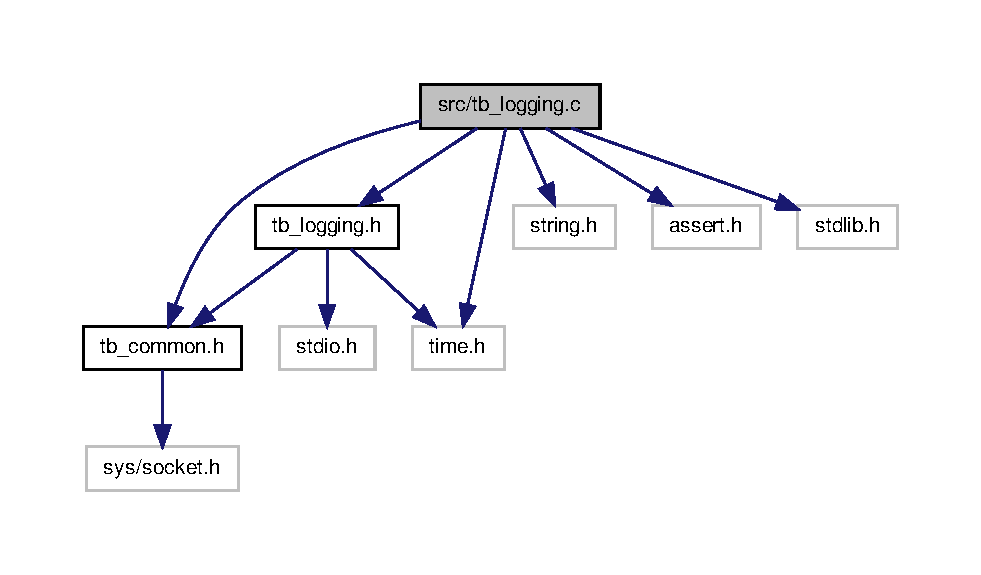
\includegraphics[width=350pt]{tb__logging_8c__incl}
\end{center}
\end{figure}
\subsection*{Functions}
\begin{DoxyCompactItemize}
\item 
\hyperlink{structtb__log__t}{tb\-\_\-log\-\_\-t} $\ast$ \hyperlink{tb__logging_8c_a7c68189d58c8f662755a184836695c8e}{tb\-\_\-create\-\_\-log} (char $\ast$file\-\_\-path)
\begin{DoxyCompactList}\small\item\em Create a log file, using a plain name. \end{DoxyCompactList}\item 
\hyperlink{structtb__log__t}{tb\-\_\-log\-\_\-t} $\ast$ \hyperlink{tb__logging_8c_aa99e3e9fc572c1967a821f2ef6065688}{tb\-\_\-create\-\_\-flog} (char $\ast$file\-\_\-path, \hyperlink{tb__logging_8h_ac6d7d82286fbda5f38dd716090016097}{tb\-\_\-log\-\_\-format\-\_\-t} format)
\begin{DoxyCompactList}\small\item\em Creat a log file, adding formatting to the log file name. \end{DoxyCompactList}\item 
void \hyperlink{tb__logging_8c_aa819c4fe320cf477fa53dc930794e475}{tb\-\_\-destroy\-\_\-log} (\hyperlink{structtb__log__t}{tb\-\_\-log\-\_\-t} $\ast$log)
\begin{DoxyCompactList}\small\item\em Destroy the log struct. \end{DoxyCompactList}\item 
int \hyperlink{tb__logging_8c_a82ad705fd902df959659c7460c4d10b9}{tb\-\_\-write\-\_\-log} (\hyperlink{structtb__log__t}{tb\-\_\-log\-\_\-t} $\ast$log, char $\ast$info, \hyperlink{tb__logging_8h_a15964dc9e84f3d4095c21137929d15c9}{tb\-\_\-log\-\_\-type\-\_\-t} type)
\begin{DoxyCompactList}\small\item\em Write a line to log file. \end{DoxyCompactList}\item 
void \hyperlink{tb__logging_8c_a407bad243d74817f840ebff158776117}{tb\-\_\-get\-\_\-f\-\_\-time} (char $\ast$time\-\_\-str, size\-\_\-t len, const char $\ast$format)
\begin{DoxyCompactList}\small\item\em Get formatted time. \end{DoxyCompactList}\end{DoxyCompactItemize}


\subsection{Function Documentation}
\hypertarget{tb__logging_8c_aa99e3e9fc572c1967a821f2ef6065688}{\index{tb\-\_\-logging.\-c@{tb\-\_\-logging.\-c}!tb\-\_\-create\-\_\-flog@{tb\-\_\-create\-\_\-flog}}
\index{tb\-\_\-create\-\_\-flog@{tb\-\_\-create\-\_\-flog}!tb_logging.c@{tb\-\_\-logging.\-c}}
\subsubsection[{tb\-\_\-create\-\_\-flog}]{\setlength{\rightskip}{0pt plus 5cm}{\bf tb\-\_\-log\-\_\-t}$\ast$ tb\-\_\-create\-\_\-flog (
\begin{DoxyParamCaption}
\item[{char $\ast$}]{file\-\_\-path, }
\item[{{\bf tb\-\_\-log\-\_\-format\-\_\-t}}]{format}
\end{DoxyParamCaption}
)}}\label{tb__logging_8c_aa99e3e9fc572c1967a821f2ef6065688}


Creat a log file, adding formatting to the log file name. 



Definition at line 33 of file tb\-\_\-logging.\-c.

\hypertarget{tb__logging_8c_a7c68189d58c8f662755a184836695c8e}{\index{tb\-\_\-logging.\-c@{tb\-\_\-logging.\-c}!tb\-\_\-create\-\_\-log@{tb\-\_\-create\-\_\-log}}
\index{tb\-\_\-create\-\_\-log@{tb\-\_\-create\-\_\-log}!tb_logging.c@{tb\-\_\-logging.\-c}}
\subsubsection[{tb\-\_\-create\-\_\-log}]{\setlength{\rightskip}{0pt plus 5cm}{\bf tb\-\_\-log\-\_\-t}$\ast$ tb\-\_\-create\-\_\-log (
\begin{DoxyParamCaption}
\item[{char $\ast$}]{file\-\_\-path}
\end{DoxyParamCaption}
)}}\label{tb__logging_8c_a7c68189d58c8f662755a184836695c8e}


Create a log file, using a plain name. 



Definition at line 18 of file tb\-\_\-logging.\-c.

\hypertarget{tb__logging_8c_aa819c4fe320cf477fa53dc930794e475}{\index{tb\-\_\-logging.\-c@{tb\-\_\-logging.\-c}!tb\-\_\-destroy\-\_\-log@{tb\-\_\-destroy\-\_\-log}}
\index{tb\-\_\-destroy\-\_\-log@{tb\-\_\-destroy\-\_\-log}!tb_logging.c@{tb\-\_\-logging.\-c}}
\subsubsection[{tb\-\_\-destroy\-\_\-log}]{\setlength{\rightskip}{0pt plus 5cm}void tb\-\_\-destroy\-\_\-log (
\begin{DoxyParamCaption}
\item[{{\bf tb\-\_\-log\-\_\-t} $\ast$}]{log}
\end{DoxyParamCaption}
)}}\label{tb__logging_8c_aa819c4fe320cf477fa53dc930794e475}


Destroy the log struct. 

Frees memory for the \hyperlink{structtb__log__t}{tb\-\_\-log\-\_\-t} struct. 

Definition at line 50 of file tb\-\_\-logging.\-c.

\hypertarget{tb__logging_8c_a407bad243d74817f840ebff158776117}{\index{tb\-\_\-logging.\-c@{tb\-\_\-logging.\-c}!tb\-\_\-get\-\_\-f\-\_\-time@{tb\-\_\-get\-\_\-f\-\_\-time}}
\index{tb\-\_\-get\-\_\-f\-\_\-time@{tb\-\_\-get\-\_\-f\-\_\-time}!tb_logging.c@{tb\-\_\-logging.\-c}}
\subsubsection[{tb\-\_\-get\-\_\-f\-\_\-time}]{\setlength{\rightskip}{0pt plus 5cm}void tb\-\_\-get\-\_\-f\-\_\-time (
\begin{DoxyParamCaption}
\item[{char $\ast$}]{time\-\_\-str, }
\item[{size\-\_\-t}]{len, }
\item[{const char $\ast$}]{format}
\end{DoxyParamCaption}
)\hspace{0.3cm}{\ttfamily [inline]}}}\label{tb__logging_8c_a407bad243d74817f840ebff158776117}


Get formatted time. 



Definition at line 116 of file tb\-\_\-logging.\-c.

\hypertarget{tb__logging_8c_a82ad705fd902df959659c7460c4d10b9}{\index{tb\-\_\-logging.\-c@{tb\-\_\-logging.\-c}!tb\-\_\-write\-\_\-log@{tb\-\_\-write\-\_\-log}}
\index{tb\-\_\-write\-\_\-log@{tb\-\_\-write\-\_\-log}!tb_logging.c@{tb\-\_\-logging.\-c}}
\subsubsection[{tb\-\_\-write\-\_\-log}]{\setlength{\rightskip}{0pt plus 5cm}int tb\-\_\-write\-\_\-log (
\begin{DoxyParamCaption}
\item[{{\bf tb\-\_\-log\-\_\-t} $\ast$}]{log, }
\item[{char $\ast$}]{info, }
\item[{{\bf tb\-\_\-log\-\_\-type\-\_\-t}}]{type}
\end{DoxyParamCaption}
)}}\label{tb__logging_8c_a82ad705fd902df959659c7460c4d10b9}


Write a line to log file. 

Writes the supplied line to the specified log file, prepending the type, date and time to this string, eg\-:

\mbox{[} I\-N\-F \mbox{]} \mbox{[} Wed Jan 29 10\-:30\-:33 2014 \mbox{]} Info 

Definition at line 58 of file tb\-\_\-logging.\-c.


\hypertarget{tb__logging_8h}{\section{src/tb\-\_\-logging.h File Reference}
\label{tb__logging_8h}\index{src/tb\-\_\-logging.\-h@{src/tb\-\_\-logging.\-h}}
}
{\ttfamily \#include $<$stdio.\-h$>$}\\*
Include dependency graph for tb\-\_\-logging.\-h\-:\nopagebreak
\begin{figure}[H]
\begin{center}
\leavevmode
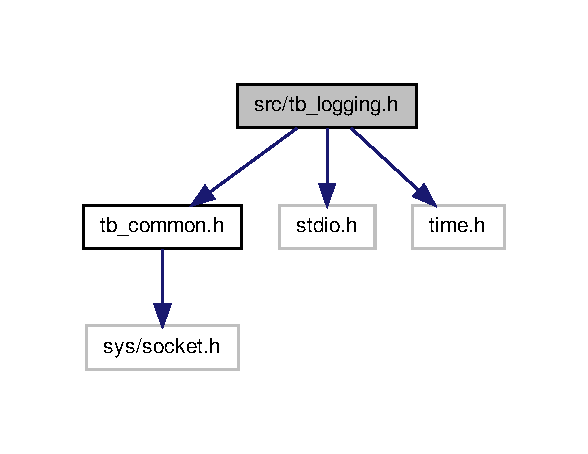
\includegraphics[width=282pt]{tb__logging_8h__incl}
\end{center}
\end{figure}
This graph shows which files directly or indirectly include this file\-:\nopagebreak
\begin{figure}[H]
\begin{center}
\leavevmode
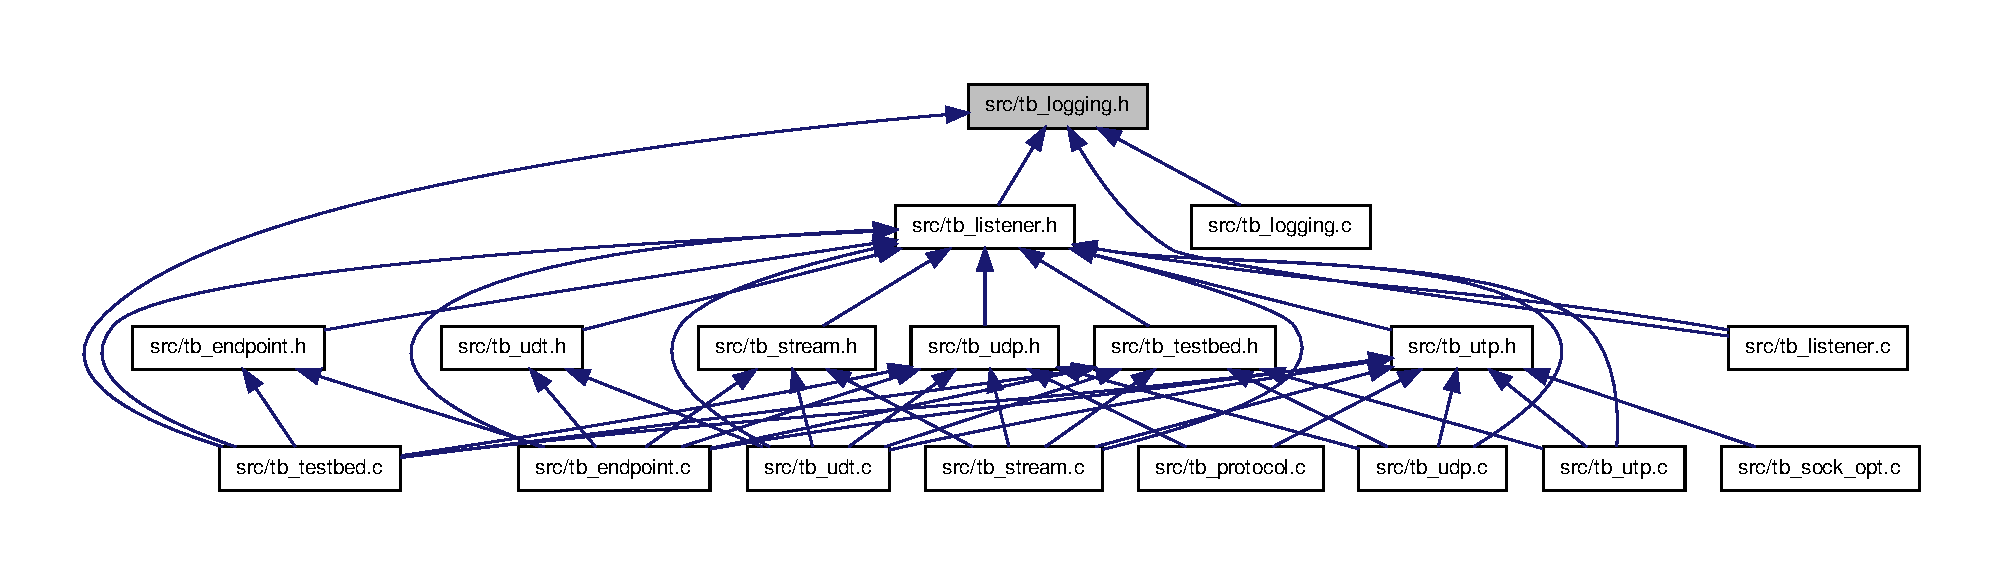
\includegraphics[width=350pt]{tb__logging_8h__dep__incl}
\end{center}
\end{figure}
\subsection*{Data Structures}
\begin{DoxyCompactItemize}
\item 
struct \hyperlink{structtb__log__t}{tb\-\_\-log\-\_\-t}
\end{DoxyCompactItemize}
\subsection*{Macros}
\begin{DoxyCompactItemize}
\item 
\#define \hyperlink{tb__logging_8h_a44e93e627399c941f83961cf839eaaf2}{L\-\_\-\-I\-N\-F\-O}~\char`\"{}\mbox{[} I\-N\-F \mbox{]}\char`\"{}
\item 
\#define \hyperlink{tb__logging_8h_a7c0f1dfbbf64536fd87f0cfcb3e68e48}{L\-\_\-\-A\-C\-K}~\char`\"{}\mbox{[} A\-C\-K \mbox{]}\char`\"{}
\item 
\#define \hyperlink{tb__logging_8h_a20994ae9abfb84898f46f5e525831a0e}{L\-\_\-\-E\-R\-R}~\char`\"{}\mbox{[} E\-R\-R \mbox{]}\char`\"{}
\end{DoxyCompactItemize}
\subsection*{Enumerations}
\begin{DoxyCompactItemize}
\item 
enum \hyperlink{tb__logging_8h_a15964dc9e84f3d4095c21137929d15c9}{tb\-\_\-log\-\_\-type\-\_\-t} \{ \hyperlink{tb__logging_8h_a15964dc9e84f3d4095c21137929d15c9a6e98ff471e3ce6c4ef2d75c37ee51837}{L\-O\-G\-\_\-\-I\-N\-F\-O} =  0, 
\hyperlink{tb__logging_8h_a15964dc9e84f3d4095c21137929d15c9aca63fedd69011a057f29a512c1a0634f}{L\-O\-G\-\_\-\-A\-C\-K}, 
\hyperlink{tb__logging_8h_a15964dc9e84f3d4095c21137929d15c9a0b4d9ad891dde7ae8deeb1704195858c}{L\-O\-G\-\_\-\-E\-R\-R}
 \}
\item 
enum \hyperlink{tb__logging_8h_ac6d7d82286fbda5f38dd716090016097}{tb\-\_\-log\-\_\-format\-\_\-t} \{ \hyperlink{tb__logging_8h_ac6d7d82286fbda5f38dd716090016097a8386f3e3e7be0b7b603636867c133a5d}{P\-L\-A\-I\-N} =  0, 
\hyperlink{tb__logging_8h_ac6d7d82286fbda5f38dd716090016097a0ace72efd9e987dfd807365d0ca50141}{D\-A\-T\-E}, 
\hyperlink{tb__logging_8h_ac6d7d82286fbda5f38dd716090016097ae9e4c627760f36823cdd153c24229157}{T\-I\-M\-E}
 \}
\end{DoxyCompactItemize}
\subsection*{Functions}
\begin{DoxyCompactItemize}
\item 
\hyperlink{structtb__log__t}{tb\-\_\-log\-\_\-t} $\ast$ \hyperlink{tb__logging_8h_a7c68189d58c8f662755a184836695c8e}{tb\-\_\-create\-\_\-log} (char $\ast$file\-\_\-path)
\begin{DoxyCompactList}\small\item\em Create a log file, using a plain name. \end{DoxyCompactList}\item 
\hyperlink{structtb__log__t}{tb\-\_\-log\-\_\-t} $\ast$ \hyperlink{tb__logging_8h_aa99e3e9fc572c1967a821f2ef6065688}{tb\-\_\-create\-\_\-flog} (char $\ast$file\-\_\-path, \hyperlink{tb__logging_8h_ac6d7d82286fbda5f38dd716090016097}{tb\-\_\-log\-\_\-format\-\_\-t} format)
\begin{DoxyCompactList}\small\item\em Creat a log file, adding formatting to the log file name. \end{DoxyCompactList}\item 
void \hyperlink{tb__logging_8h_aa819c4fe320cf477fa53dc930794e475}{tb\-\_\-destroy\-\_\-log} (\hyperlink{structtb__log__t}{tb\-\_\-log\-\_\-t} $\ast$log)
\begin{DoxyCompactList}\small\item\em Destroy the log struct. \end{DoxyCompactList}\item 
int \hyperlink{tb__logging_8h_a82ad705fd902df959659c7460c4d10b9}{tb\-\_\-write\-\_\-log} (\hyperlink{structtb__log__t}{tb\-\_\-log\-\_\-t} $\ast$log, char $\ast$info, \hyperlink{tb__logging_8h_a15964dc9e84f3d4095c21137929d15c9}{tb\-\_\-log\-\_\-type\-\_\-t} type)
\begin{DoxyCompactList}\small\item\em Write a line to log file. \end{DoxyCompactList}\item 
void \hyperlink{tb__logging_8h_af988d5c63ebae79e18dc2cd96ab3821c}{tb\-\_\-get\-\_\-f\-\_\-time} (char $\ast$time\-\_\-str, size\-\_\-t len, const char $\ast$format) \-\_\-\-\_\-attribute\-\_\-\-\_\-((always\-\_\-inline))
\begin{DoxyCompactList}\small\item\em Get formatted time. \end{DoxyCompactList}\end{DoxyCompactItemize}


\subsection{Macro Definition Documentation}
\hypertarget{tb__logging_8h_a7c0f1dfbbf64536fd87f0cfcb3e68e48}{\index{tb\-\_\-logging.\-h@{tb\-\_\-logging.\-h}!L\-\_\-\-A\-C\-K@{L\-\_\-\-A\-C\-K}}
\index{L\-\_\-\-A\-C\-K@{L\-\_\-\-A\-C\-K}!tb_logging.h@{tb\-\_\-logging.\-h}}
\subsubsection[{L\-\_\-\-A\-C\-K}]{\setlength{\rightskip}{0pt plus 5cm}\#define L\-\_\-\-A\-C\-K~\char`\"{}\mbox{[} A\-C\-K \mbox{]}\char`\"{}}}\label{tb__logging_8h_a7c0f1dfbbf64536fd87f0cfcb3e68e48}


Definition at line 14 of file tb\-\_\-logging.\-h.

\hypertarget{tb__logging_8h_a20994ae9abfb84898f46f5e525831a0e}{\index{tb\-\_\-logging.\-h@{tb\-\_\-logging.\-h}!L\-\_\-\-E\-R\-R@{L\-\_\-\-E\-R\-R}}
\index{L\-\_\-\-E\-R\-R@{L\-\_\-\-E\-R\-R}!tb_logging.h@{tb\-\_\-logging.\-h}}
\subsubsection[{L\-\_\-\-E\-R\-R}]{\setlength{\rightskip}{0pt plus 5cm}\#define L\-\_\-\-E\-R\-R~\char`\"{}\mbox{[} E\-R\-R \mbox{]}\char`\"{}}}\label{tb__logging_8h_a20994ae9abfb84898f46f5e525831a0e}


Definition at line 15 of file tb\-\_\-logging.\-h.

\hypertarget{tb__logging_8h_a44e93e627399c941f83961cf839eaaf2}{\index{tb\-\_\-logging.\-h@{tb\-\_\-logging.\-h}!L\-\_\-\-I\-N\-F\-O@{L\-\_\-\-I\-N\-F\-O}}
\index{L\-\_\-\-I\-N\-F\-O@{L\-\_\-\-I\-N\-F\-O}!tb_logging.h@{tb\-\_\-logging.\-h}}
\subsubsection[{L\-\_\-\-I\-N\-F\-O}]{\setlength{\rightskip}{0pt plus 5cm}\#define L\-\_\-\-I\-N\-F\-O~\char`\"{}\mbox{[} I\-N\-F \mbox{]}\char`\"{}}}\label{tb__logging_8h_a44e93e627399c941f83961cf839eaaf2}


Definition at line 13 of file tb\-\_\-logging.\-h.



\subsection{Enumeration Type Documentation}
\hypertarget{tb__logging_8h_ac6d7d82286fbda5f38dd716090016097}{\index{tb\-\_\-logging.\-h@{tb\-\_\-logging.\-h}!tb\-\_\-log\-\_\-format\-\_\-t@{tb\-\_\-log\-\_\-format\-\_\-t}}
\index{tb\-\_\-log\-\_\-format\-\_\-t@{tb\-\_\-log\-\_\-format\-\_\-t}!tb_logging.h@{tb\-\_\-logging.\-h}}
\subsubsection[{tb\-\_\-log\-\_\-format\-\_\-t}]{\setlength{\rightskip}{0pt plus 5cm}enum {\bf tb\-\_\-log\-\_\-format\-\_\-t}}}\label{tb__logging_8h_ac6d7d82286fbda5f38dd716090016097}
\begin{Desc}
\item[Enumerator\-: ]\par
\begin{description}
\index{P\-L\-A\-I\-N@{P\-L\-A\-I\-N}!tb\-\_\-logging.\-h@{tb\-\_\-logging.\-h}}\index{tb\-\_\-logging.\-h@{tb\-\_\-logging.\-h}!P\-L\-A\-I\-N@{P\-L\-A\-I\-N}}\item[{\em 
\hypertarget{tb__logging_8h_ac6d7d82286fbda5f38dd716090016097a8386f3e3e7be0b7b603636867c133a5d}{P\-L\-A\-I\-N}\label{tb__logging_8h_ac6d7d82286fbda5f38dd716090016097a8386f3e3e7be0b7b603636867c133a5d}
}]\index{D\-A\-T\-E@{D\-A\-T\-E}!tb\-\_\-logging.\-h@{tb\-\_\-logging.\-h}}\index{tb\-\_\-logging.\-h@{tb\-\_\-logging.\-h}!D\-A\-T\-E@{D\-A\-T\-E}}\item[{\em 
\hypertarget{tb__logging_8h_ac6d7d82286fbda5f38dd716090016097a0ace72efd9e987dfd807365d0ca50141}{D\-A\-T\-E}\label{tb__logging_8h_ac6d7d82286fbda5f38dd716090016097a0ace72efd9e987dfd807365d0ca50141}
}]\index{T\-I\-M\-E@{T\-I\-M\-E}!tb\-\_\-logging.\-h@{tb\-\_\-logging.\-h}}\index{tb\-\_\-logging.\-h@{tb\-\_\-logging.\-h}!T\-I\-M\-E@{T\-I\-M\-E}}\item[{\em 
\hypertarget{tb__logging_8h_ac6d7d82286fbda5f38dd716090016097ae9e4c627760f36823cdd153c24229157}{T\-I\-M\-E}\label{tb__logging_8h_ac6d7d82286fbda5f38dd716090016097ae9e4c627760f36823cdd153c24229157}
}]\end{description}
\end{Desc}



Definition at line 33 of file tb\-\_\-logging.\-h.

\hypertarget{tb__logging_8h_a15964dc9e84f3d4095c21137929d15c9}{\index{tb\-\_\-logging.\-h@{tb\-\_\-logging.\-h}!tb\-\_\-log\-\_\-type\-\_\-t@{tb\-\_\-log\-\_\-type\-\_\-t}}
\index{tb\-\_\-log\-\_\-type\-\_\-t@{tb\-\_\-log\-\_\-type\-\_\-t}!tb_logging.h@{tb\-\_\-logging.\-h}}
\subsubsection[{tb\-\_\-log\-\_\-type\-\_\-t}]{\setlength{\rightskip}{0pt plus 5cm}enum {\bf tb\-\_\-log\-\_\-type\-\_\-t}}}\label{tb__logging_8h_a15964dc9e84f3d4095c21137929d15c9}
\begin{Desc}
\item[Enumerator\-: ]\par
\begin{description}
\index{L\-O\-G\-\_\-\-I\-N\-F\-O@{L\-O\-G\-\_\-\-I\-N\-F\-O}!tb\-\_\-logging.\-h@{tb\-\_\-logging.\-h}}\index{tb\-\_\-logging.\-h@{tb\-\_\-logging.\-h}!L\-O\-G\-\_\-\-I\-N\-F\-O@{L\-O\-G\-\_\-\-I\-N\-F\-O}}\item[{\em 
\hypertarget{tb__logging_8h_a15964dc9e84f3d4095c21137929d15c9a6e98ff471e3ce6c4ef2d75c37ee51837}{L\-O\-G\-\_\-\-I\-N\-F\-O}\label{tb__logging_8h_a15964dc9e84f3d4095c21137929d15c9a6e98ff471e3ce6c4ef2d75c37ee51837}
}]\index{L\-O\-G\-\_\-\-A\-C\-K@{L\-O\-G\-\_\-\-A\-C\-K}!tb\-\_\-logging.\-h@{tb\-\_\-logging.\-h}}\index{tb\-\_\-logging.\-h@{tb\-\_\-logging.\-h}!L\-O\-G\-\_\-\-A\-C\-K@{L\-O\-G\-\_\-\-A\-C\-K}}\item[{\em 
\hypertarget{tb__logging_8h_a15964dc9e84f3d4095c21137929d15c9aca63fedd69011a057f29a512c1a0634f}{L\-O\-G\-\_\-\-A\-C\-K}\label{tb__logging_8h_a15964dc9e84f3d4095c21137929d15c9aca63fedd69011a057f29a512c1a0634f}
}]\index{L\-O\-G\-\_\-\-E\-R\-R@{L\-O\-G\-\_\-\-E\-R\-R}!tb\-\_\-logging.\-h@{tb\-\_\-logging.\-h}}\index{tb\-\_\-logging.\-h@{tb\-\_\-logging.\-h}!L\-O\-G\-\_\-\-E\-R\-R@{L\-O\-G\-\_\-\-E\-R\-R}}\item[{\em 
\hypertarget{tb__logging_8h_a15964dc9e84f3d4095c21137929d15c9a0b4d9ad891dde7ae8deeb1704195858c}{L\-O\-G\-\_\-\-E\-R\-R}\label{tb__logging_8h_a15964dc9e84f3d4095c21137929d15c9a0b4d9ad891dde7ae8deeb1704195858c}
}]\end{description}
\end{Desc}



Definition at line 25 of file tb\-\_\-logging.\-h.



\subsection{Function Documentation}
\hypertarget{tb__logging_8h_aa99e3e9fc572c1967a821f2ef6065688}{\index{tb\-\_\-logging.\-h@{tb\-\_\-logging.\-h}!tb\-\_\-create\-\_\-flog@{tb\-\_\-create\-\_\-flog}}
\index{tb\-\_\-create\-\_\-flog@{tb\-\_\-create\-\_\-flog}!tb_logging.h@{tb\-\_\-logging.\-h}}
\subsubsection[{tb\-\_\-create\-\_\-flog}]{\setlength{\rightskip}{0pt plus 5cm}{\bf tb\-\_\-log\-\_\-t}$\ast$ tb\-\_\-create\-\_\-flog (
\begin{DoxyParamCaption}
\item[{char $\ast$}]{file\-\_\-path, }
\item[{{\bf tb\-\_\-log\-\_\-format\-\_\-t}}]{format}
\end{DoxyParamCaption}
)}}\label{tb__logging_8h_aa99e3e9fc572c1967a821f2ef6065688}


Creat a log file, adding formatting to the log file name. 



Definition at line 33 of file tb\-\_\-logging.\-c.

\hypertarget{tb__logging_8h_a7c68189d58c8f662755a184836695c8e}{\index{tb\-\_\-logging.\-h@{tb\-\_\-logging.\-h}!tb\-\_\-create\-\_\-log@{tb\-\_\-create\-\_\-log}}
\index{tb\-\_\-create\-\_\-log@{tb\-\_\-create\-\_\-log}!tb_logging.h@{tb\-\_\-logging.\-h}}
\subsubsection[{tb\-\_\-create\-\_\-log}]{\setlength{\rightskip}{0pt plus 5cm}{\bf tb\-\_\-log\-\_\-t}$\ast$ tb\-\_\-create\-\_\-log (
\begin{DoxyParamCaption}
\item[{char $\ast$}]{file\-\_\-path}
\end{DoxyParamCaption}
)}}\label{tb__logging_8h_a7c68189d58c8f662755a184836695c8e}


Create a log file, using a plain name. 



Definition at line 18 of file tb\-\_\-logging.\-c.

\hypertarget{tb__logging_8h_aa819c4fe320cf477fa53dc930794e475}{\index{tb\-\_\-logging.\-h@{tb\-\_\-logging.\-h}!tb\-\_\-destroy\-\_\-log@{tb\-\_\-destroy\-\_\-log}}
\index{tb\-\_\-destroy\-\_\-log@{tb\-\_\-destroy\-\_\-log}!tb_logging.h@{tb\-\_\-logging.\-h}}
\subsubsection[{tb\-\_\-destroy\-\_\-log}]{\setlength{\rightskip}{0pt plus 5cm}void tb\-\_\-destroy\-\_\-log (
\begin{DoxyParamCaption}
\item[{{\bf tb\-\_\-log\-\_\-t} $\ast$}]{log}
\end{DoxyParamCaption}
)}}\label{tb__logging_8h_aa819c4fe320cf477fa53dc930794e475}


Destroy the log struct. 

Frees memory for the \hyperlink{structtb__log__t}{tb\-\_\-log\-\_\-t} struct. 

Definition at line 50 of file tb\-\_\-logging.\-c.

\hypertarget{tb__logging_8h_af988d5c63ebae79e18dc2cd96ab3821c}{\index{tb\-\_\-logging.\-h@{tb\-\_\-logging.\-h}!tb\-\_\-get\-\_\-f\-\_\-time@{tb\-\_\-get\-\_\-f\-\_\-time}}
\index{tb\-\_\-get\-\_\-f\-\_\-time@{tb\-\_\-get\-\_\-f\-\_\-time}!tb_logging.h@{tb\-\_\-logging.\-h}}
\subsubsection[{tb\-\_\-get\-\_\-f\-\_\-time}]{\setlength{\rightskip}{0pt plus 5cm}void tb\-\_\-get\-\_\-f\-\_\-time (
\begin{DoxyParamCaption}
\item[{char $\ast$}]{time\-\_\-str, }
\item[{size\-\_\-t}]{len, }
\item[{const char $\ast$}]{format}
\end{DoxyParamCaption}
)\hspace{0.3cm}{\ttfamily [inline]}}}\label{tb__logging_8h_af988d5c63ebae79e18dc2cd96ab3821c}


Get formatted time. 



Definition at line 116 of file tb\-\_\-logging.\-c.

\hypertarget{tb__logging_8h_a82ad705fd902df959659c7460c4d10b9}{\index{tb\-\_\-logging.\-h@{tb\-\_\-logging.\-h}!tb\-\_\-write\-\_\-log@{tb\-\_\-write\-\_\-log}}
\index{tb\-\_\-write\-\_\-log@{tb\-\_\-write\-\_\-log}!tb_logging.h@{tb\-\_\-logging.\-h}}
\subsubsection[{tb\-\_\-write\-\_\-log}]{\setlength{\rightskip}{0pt plus 5cm}int tb\-\_\-write\-\_\-log (
\begin{DoxyParamCaption}
\item[{{\bf tb\-\_\-log\-\_\-t} $\ast$}]{log, }
\item[{char $\ast$}]{info, }
\item[{{\bf tb\-\_\-log\-\_\-type\-\_\-t}}]{type}
\end{DoxyParamCaption}
)}}\label{tb__logging_8h_a82ad705fd902df959659c7460c4d10b9}


Write a line to log file. 

Writes the supplied line to the specified log file, prepending the type, date and time to this string, eg\-:

\mbox{[} I\-N\-F \mbox{]} \mbox{[} Wed Jan 29 10\-:30\-:33 2014 \mbox{]} Info 

Definition at line 58 of file tb\-\_\-logging.\-c.


\hypertarget{tb__protocol_8c}{\section{src/tb\-\_\-protocol.c File Reference}
\label{tb__protocol_8c}\index{src/tb\-\_\-protocol.\-c@{src/tb\-\_\-protocol.\-c}}
}
{\ttfamily \#include \char`\"{}tb\-\_\-protocol.\-h\char`\"{}}\\*
{\ttfamily \#include \char`\"{}tb\-\_\-utp.\-h\char`\"{}}\\*
{\ttfamily \#include \char`\"{}tb\-\_\-udp.\-h\char`\"{}}\\*
{\ttfamily \#include \char`\"{}tb\-\_\-common.\-h\char`\"{}}\\*
{\ttfamily \#include $<$sys/socket.\-h$>$}\\*
{\ttfamily \#include $<$stdlib.\-h$>$}\\*
{\ttfamily \#include $<$udt.\-h$>$}\\*
{\ttfamily \#include $<$utp.\-h$>$}\\*
{\ttfamily \#include $<$unistd.\-h$>$}\\*
{\ttfamily \#include $<$stdio.\-h$>$}\\*
{\ttfamily \#include $<$fcntl.\-h$>$}\\*
{\ttfamily \#include $<$netinet/tcp.\-h$>$}\\*
{\ttfamily \#include $<$errno.\-h$>$}\\*
{\ttfamily \#include $<$string.\-h$>$}\\*
Include dependency graph for tb\-\_\-protocol.\-c\-:\nopagebreak
\begin{figure}[H]
\begin{center}
\leavevmode
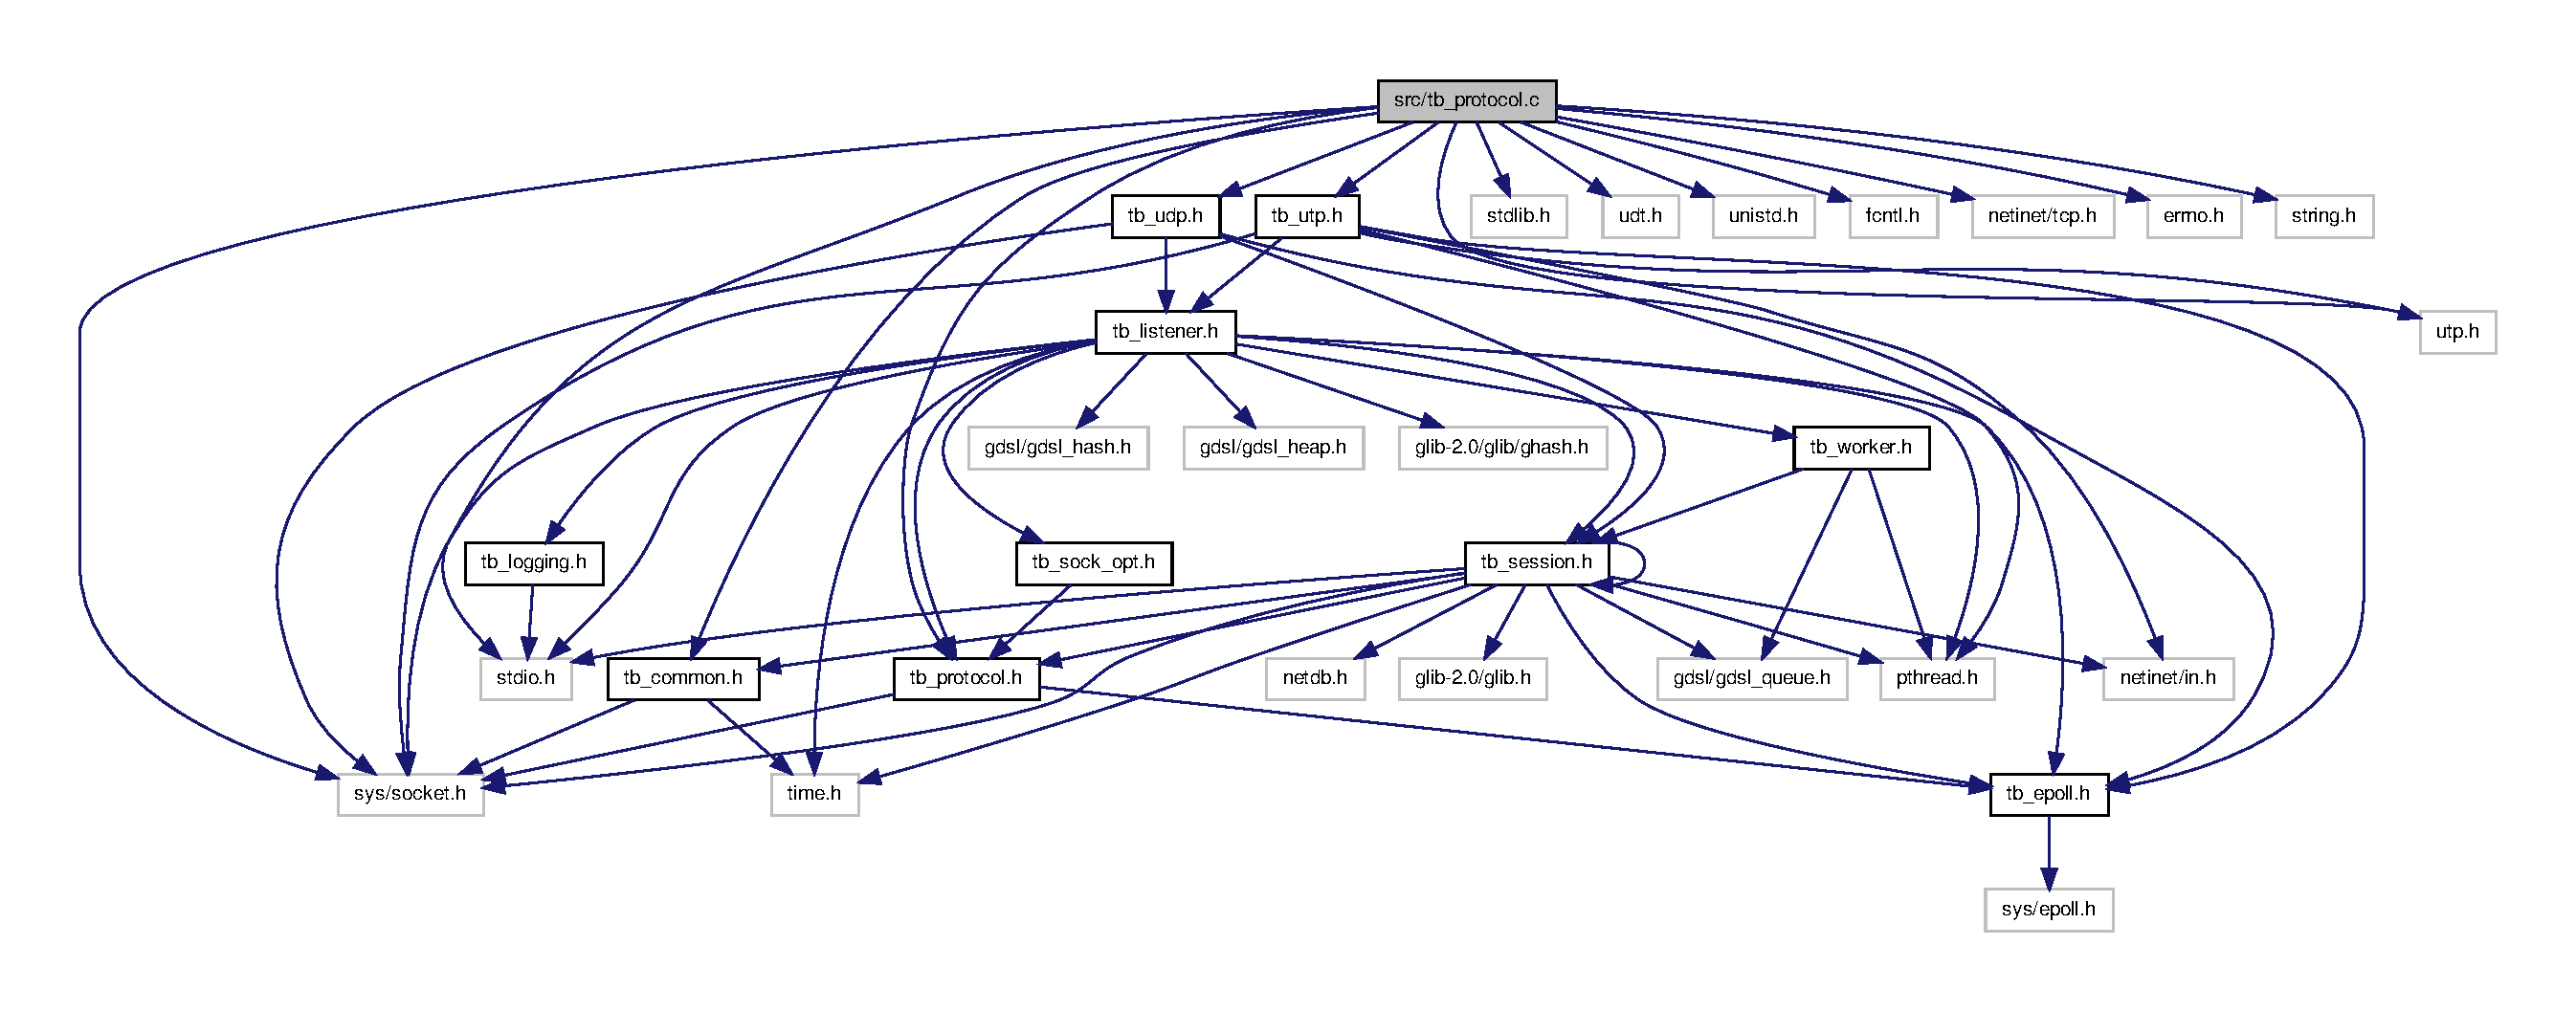
\includegraphics[width=350pt]{tb__protocol_8c__incl}
\end{center}
\end{figure}
\subsection*{Functions}
\begin{DoxyCompactItemize}
\item 
\hyperlink{structtb__protocol__t}{tb\-\_\-protocol\-\_\-t} $\ast$ \hyperlink{tb__protocol_8c_aa906a171c2fff5aaf32df7b087153ea0}{tb\-\_\-create\-\_\-protocol} (\hyperlink{tb__protocol_8h_a7a5bff1040fc154c510874327d44cc1a}{P\-R\-O\-T\-O\-C\-O\-L} prot)
\begin{DoxyCompactList}\small\item\em Create a new Protocol. \end{DoxyCompactList}\item 
int \hyperlink{tb__protocol_8c_aabab4d45d896ccb2520e32d2da0a0844}{tb\-\_\-socket\-\_\-error} (int value, int err\-\_\-no)
\begin{DoxyCompactList}\small\item\em Handle errors for socket. \end{DoxyCompactList}\item 
int \hyperlink{tb__protocol_8c_a773702577cc5960a28390c6d2c637679}{tb\-\_\-dccp\-\_\-error} (int value, int err\-\_\-no)
\begin{DoxyCompactList}\small\item\em Handle errors for dccp. \end{DoxyCompactList}\item 
int \hyperlink{tb__protocol_8c_a634f0d467979a16f779333c4f00f97cf}{tb\-\_\-udt\-\_\-error} (int value, int err\-\_\-no)
\begin{DoxyCompactList}\small\item\em Handle errors for udt. \end{DoxyCompactList}\item 
void \hyperlink{tb__protocol_8c_aa2b5480d4df920972d7dec20c54ddfe9}{tb\-\_\-print\-\_\-protocol} (\hyperlink{structtb__protocol__t}{tb\-\_\-protocol\-\_\-t} $\ast$protocol)
\begin{DoxyCompactList}\small\item\em Print the values for this protocol. \end{DoxyCompactList}\item 
void \hyperlink{tb__protocol_8c_a5f8e49b8ee3a8b874dd58231dd099de1}{tb\-\_\-get\-\_\-stats} (\hyperlink{structtb__prot__stats__t}{tb\-\_\-prot\-\_\-stats\-\_\-t} $\ast$stats, int fd)
\begin{DoxyCompactList}\small\item\em Get the stats for the given protocol, with the given descriptor. \end{DoxyCompactList}\item 
void \hyperlink{tb__protocol_8c_aebf261998277b8c36c9b827a3cb2f69a}{tb\-\_\-destroy\-\_\-stats} (\hyperlink{structtb__prot__stats__t}{tb\-\_\-prot\-\_\-stats\-\_\-t} $\ast$stats)
\begin{DoxyCompactList}\small\item\em Destroy stats struct. \end{DoxyCompactList}\item 
void \hyperlink{tb__protocol_8c_a8e38a6ede656010fb440c895610a5d10}{get\-\_\-udt\-\_\-stats} (\hyperlink{structtb__prot__stats__t}{tb\-\_\-prot\-\_\-stats\-\_\-t} $\ast$stats, int fd)
\begin{DoxyCompactList}\small\item\em Get udt stats. \end{DoxyCompactList}\item 
void \hyperlink{tb__protocol_8c_a70096149add47bfaceb6a1c893a9dfd1}{get\-\_\-udp\-\_\-stats} (\hyperlink{structtb__prot__stats__t}{tb\-\_\-prot\-\_\-stats\-\_\-t} $\ast$stats, int fd)
\begin{DoxyCompactList}\small\item\em Get udp stats. \end{DoxyCompactList}\item 
void \hyperlink{tb__protocol_8c_ae303c4e113a72eb8daf629260f13c5a3}{get\-\_\-utp\-\_\-stats} (\hyperlink{structtb__prot__stats__t}{tb\-\_\-prot\-\_\-stats\-\_\-t} $\ast$stats, int fd)
\begin{DoxyCompactList}\small\item\em Get utp stats. \end{DoxyCompactList}\item 
void \hyperlink{tb__protocol_8c_ad16e59fe4e10eb09b2aa2d190baab34e}{get\-\_\-dccp\-\_\-stats} (\hyperlink{structtb__prot__stats__t}{tb\-\_\-prot\-\_\-stats\-\_\-t} $\ast$stats, int fd)
\begin{DoxyCompactList}\small\item\em Get dccp stats. \end{DoxyCompactList}\item 
void \hyperlink{tb__protocol_8c_a8f184a229468afe5ccaa51621032fea5}{get\-\_\-tcp\-\_\-stats} (\hyperlink{structtb__prot__stats__t}{tb\-\_\-prot\-\_\-stats\-\_\-t} $\ast$stats, int fd)
\begin{DoxyCompactList}\small\item\em Get tcp stats. \end{DoxyCompactList}\item 
void \hyperlink{tb__protocol_8c_a94412470e6630d5350bf784a827034c8}{tb\-\_\-get\-\_\-bsd\-\_\-stats} (\hyperlink{structtb__prot__stats__t}{tb\-\_\-prot\-\_\-stats\-\_\-t} $\ast$stats, int fd)
\begin{DoxyCompactList}\small\item\em Get generic bsd stats. \end{DoxyCompactList}\item 
void \hyperlink{tb__protocol_8c_a151f709ceb08d76f790638d9f2c55f37}{tb\-\_\-destroy\-\_\-protocol} (\hyperlink{structtb__protocol__t}{tb\-\_\-protocol\-\_\-t} $\ast$protocol)
\begin{DoxyCompactList}\small\item\em Destroy the given protocol structure. \end{DoxyCompactList}\end{DoxyCompactItemize}
\subsection*{Variables}
\begin{DoxyCompactItemize}
\item 
const int \hyperlink{tb__protocol_8c_adaa45d502fac3ba218461835d3391c5c}{socket\-\_\-error} = -\/1
\end{DoxyCompactItemize}


\subsection{Function Documentation}
\hypertarget{tb__protocol_8c_ad16e59fe4e10eb09b2aa2d190baab34e}{\index{tb\-\_\-protocol.\-c@{tb\-\_\-protocol.\-c}!get\-\_\-dccp\-\_\-stats@{get\-\_\-dccp\-\_\-stats}}
\index{get\-\_\-dccp\-\_\-stats@{get\-\_\-dccp\-\_\-stats}!tb_protocol.c@{tb\-\_\-protocol.\-c}}
\subsubsection[{get\-\_\-dccp\-\_\-stats}]{\setlength{\rightskip}{0pt plus 5cm}void get\-\_\-dccp\-\_\-stats (
\begin{DoxyParamCaption}
\item[{{\bf tb\-\_\-prot\-\_\-stats\-\_\-t} $\ast$}]{stats, }
\item[{int}]{fd}
\end{DoxyParamCaption}
)}}\label{tb__protocol_8c_ad16e59fe4e10eb09b2aa2d190baab34e}


Get dccp stats. 



Definition at line 299 of file tb\-\_\-protocol.\-c.

\hypertarget{tb__protocol_8c_a8f184a229468afe5ccaa51621032fea5}{\index{tb\-\_\-protocol.\-c@{tb\-\_\-protocol.\-c}!get\-\_\-tcp\-\_\-stats@{get\-\_\-tcp\-\_\-stats}}
\index{get\-\_\-tcp\-\_\-stats@{get\-\_\-tcp\-\_\-stats}!tb_protocol.c@{tb\-\_\-protocol.\-c}}
\subsubsection[{get\-\_\-tcp\-\_\-stats}]{\setlength{\rightskip}{0pt plus 5cm}void get\-\_\-tcp\-\_\-stats (
\begin{DoxyParamCaption}
\item[{{\bf tb\-\_\-prot\-\_\-stats\-\_\-t} $\ast$}]{stats, }
\item[{int}]{fd}
\end{DoxyParamCaption}
)}}\label{tb__protocol_8c_a8f184a229468afe5ccaa51621032fea5}


Get tcp stats. 



Definition at line 305 of file tb\-\_\-protocol.\-c.

\hypertarget{tb__protocol_8c_a70096149add47bfaceb6a1c893a9dfd1}{\index{tb\-\_\-protocol.\-c@{tb\-\_\-protocol.\-c}!get\-\_\-udp\-\_\-stats@{get\-\_\-udp\-\_\-stats}}
\index{get\-\_\-udp\-\_\-stats@{get\-\_\-udp\-\_\-stats}!tb_protocol.c@{tb\-\_\-protocol.\-c}}
\subsubsection[{get\-\_\-udp\-\_\-stats}]{\setlength{\rightskip}{0pt plus 5cm}void get\-\_\-udp\-\_\-stats (
\begin{DoxyParamCaption}
\item[{{\bf tb\-\_\-prot\-\_\-stats\-\_\-t} $\ast$}]{stats, }
\item[{int}]{fd}
\end{DoxyParamCaption}
)}}\label{tb__protocol_8c_a70096149add47bfaceb6a1c893a9dfd1}


Get udp stats. 



Definition at line 287 of file tb\-\_\-protocol.\-c.

\hypertarget{tb__protocol_8c_a8e38a6ede656010fb440c895610a5d10}{\index{tb\-\_\-protocol.\-c@{tb\-\_\-protocol.\-c}!get\-\_\-udt\-\_\-stats@{get\-\_\-udt\-\_\-stats}}
\index{get\-\_\-udt\-\_\-stats@{get\-\_\-udt\-\_\-stats}!tb_protocol.c@{tb\-\_\-protocol.\-c}}
\subsubsection[{get\-\_\-udt\-\_\-stats}]{\setlength{\rightskip}{0pt plus 5cm}void get\-\_\-udt\-\_\-stats (
\begin{DoxyParamCaption}
\item[{{\bf tb\-\_\-prot\-\_\-stats\-\_\-t} $\ast$}]{stats, }
\item[{int}]{fd}
\end{DoxyParamCaption}
)}}\label{tb__protocol_8c_a8e38a6ede656010fb440c895610a5d10}


Get udt stats. 



Definition at line 258 of file tb\-\_\-protocol.\-c.

\hypertarget{tb__protocol_8c_ae303c4e113a72eb8daf629260f13c5a3}{\index{tb\-\_\-protocol.\-c@{tb\-\_\-protocol.\-c}!get\-\_\-utp\-\_\-stats@{get\-\_\-utp\-\_\-stats}}
\index{get\-\_\-utp\-\_\-stats@{get\-\_\-utp\-\_\-stats}!tb_protocol.c@{tb\-\_\-protocol.\-c}}
\subsubsection[{get\-\_\-utp\-\_\-stats}]{\setlength{\rightskip}{0pt plus 5cm}void get\-\_\-utp\-\_\-stats (
\begin{DoxyParamCaption}
\item[{{\bf tb\-\_\-prot\-\_\-stats\-\_\-t} $\ast$}]{stats, }
\item[{int}]{fd}
\end{DoxyParamCaption}
)}}\label{tb__protocol_8c_ae303c4e113a72eb8daf629260f13c5a3}


Get utp stats. 



Definition at line 293 of file tb\-\_\-protocol.\-c.

\hypertarget{tb__protocol_8c_aa906a171c2fff5aaf32df7b087153ea0}{\index{tb\-\_\-protocol.\-c@{tb\-\_\-protocol.\-c}!tb\-\_\-create\-\_\-protocol@{tb\-\_\-create\-\_\-protocol}}
\index{tb\-\_\-create\-\_\-protocol@{tb\-\_\-create\-\_\-protocol}!tb_protocol.c@{tb\-\_\-protocol.\-c}}
\subsubsection[{tb\-\_\-create\-\_\-protocol}]{\setlength{\rightskip}{0pt plus 5cm}{\bf tb\-\_\-protocol\-\_\-t}$\ast$ tb\-\_\-create\-\_\-protocol (
\begin{DoxyParamCaption}
\item[{{\bf P\-R\-O\-T\-O\-C\-O\-L}}]{prot}
\end{DoxyParamCaption}
)}}\label{tb__protocol_8c_aa906a171c2fff5aaf32df7b087153ea0}


Create a new Protocol. 

Creates the protocol, and loads the struct with all of the relevant functions to perform communication.

\begin{DoxyPrecond}{Precondition}
The protocol must be one of the supported types. 
\end{DoxyPrecond}

\begin{DoxyParams}{Parameters}
{\em prot} & The protocol to use in the tests. \\
\hline
\end{DoxyParams}
\begin{DoxyReturn}{Returns}
The struct \hyperlink{structtb__protocol__t}{tb\-\_\-protocol\-\_\-t} 
\end{DoxyReturn}


Definition at line 27 of file tb\-\_\-protocol.\-c.

\hypertarget{tb__protocol_8c_a773702577cc5960a28390c6d2c637679}{\index{tb\-\_\-protocol.\-c@{tb\-\_\-protocol.\-c}!tb\-\_\-dccp\-\_\-error@{tb\-\_\-dccp\-\_\-error}}
\index{tb\-\_\-dccp\-\_\-error@{tb\-\_\-dccp\-\_\-error}!tb_protocol.c@{tb\-\_\-protocol.\-c}}
\subsubsection[{tb\-\_\-dccp\-\_\-error}]{\setlength{\rightskip}{0pt plus 5cm}int tb\-\_\-dccp\-\_\-error (
\begin{DoxyParamCaption}
\item[{int}]{value, }
\item[{int}]{err\-\_\-no}
\end{DoxyParamCaption}
)}}\label{tb__protocol_8c_a773702577cc5960a28390c6d2c637679}


Handle errors for dccp. 



Definition at line 192 of file tb\-\_\-protocol.\-c.

\hypertarget{tb__protocol_8c_a151f709ceb08d76f790638d9f2c55f37}{\index{tb\-\_\-protocol.\-c@{tb\-\_\-protocol.\-c}!tb\-\_\-destroy\-\_\-protocol@{tb\-\_\-destroy\-\_\-protocol}}
\index{tb\-\_\-destroy\-\_\-protocol@{tb\-\_\-destroy\-\_\-protocol}!tb_protocol.c@{tb\-\_\-protocol.\-c}}
\subsubsection[{tb\-\_\-destroy\-\_\-protocol}]{\setlength{\rightskip}{0pt plus 5cm}void tb\-\_\-destroy\-\_\-protocol (
\begin{DoxyParamCaption}
\item[{{\bf tb\-\_\-protocol\-\_\-t} $\ast$}]{protocol}
\end{DoxyParamCaption}
)}}\label{tb__protocol_8c_a151f709ceb08d76f790638d9f2c55f37}


Destroy the given protocol structure. 

Destroys the struct, freeing up memory.

\begin{DoxyPrecond}{Precondition}
protocol must be of type \hyperlink{structtb__protocol__t}{tb\-\_\-protocol\-\_\-t}. 
\end{DoxyPrecond}

\begin{DoxyParams}{Parameters}
{\em protocol} & The struct to destroy. \\
\hline
\end{DoxyParams}


Definition at line 344 of file tb\-\_\-protocol.\-c.

\hypertarget{tb__protocol_8c_aebf261998277b8c36c9b827a3cb2f69a}{\index{tb\-\_\-protocol.\-c@{tb\-\_\-protocol.\-c}!tb\-\_\-destroy\-\_\-stats@{tb\-\_\-destroy\-\_\-stats}}
\index{tb\-\_\-destroy\-\_\-stats@{tb\-\_\-destroy\-\_\-stats}!tb_protocol.c@{tb\-\_\-protocol.\-c}}
\subsubsection[{tb\-\_\-destroy\-\_\-stats}]{\setlength{\rightskip}{0pt plus 5cm}void tb\-\_\-destroy\-\_\-stats (
\begin{DoxyParamCaption}
\item[{{\bf tb\-\_\-prot\-\_\-stats\-\_\-t} $\ast$}]{stats}
\end{DoxyParamCaption}
)}}\label{tb__protocol_8c_aebf261998277b8c36c9b827a3cb2f69a}


Destroy stats struct. 



Definition at line 247 of file tb\-\_\-protocol.\-c.

\hypertarget{tb__protocol_8c_a94412470e6630d5350bf784a827034c8}{\index{tb\-\_\-protocol.\-c@{tb\-\_\-protocol.\-c}!tb\-\_\-get\-\_\-bsd\-\_\-stats@{tb\-\_\-get\-\_\-bsd\-\_\-stats}}
\index{tb\-\_\-get\-\_\-bsd\-\_\-stats@{tb\-\_\-get\-\_\-bsd\-\_\-stats}!tb_protocol.c@{tb\-\_\-protocol.\-c}}
\subsubsection[{tb\-\_\-get\-\_\-bsd\-\_\-stats}]{\setlength{\rightskip}{0pt plus 5cm}void tb\-\_\-get\-\_\-bsd\-\_\-stats (
\begin{DoxyParamCaption}
\item[{{\bf tb\-\_\-prot\-\_\-stats\-\_\-t} $\ast$}]{stats, }
\item[{int}]{fd}
\end{DoxyParamCaption}
)}}\label{tb__protocol_8c_a94412470e6630d5350bf784a827034c8}


Get generic bsd stats. 



Definition at line 334 of file tb\-\_\-protocol.\-c.

\hypertarget{tb__protocol_8c_a5f8e49b8ee3a8b874dd58231dd099de1}{\index{tb\-\_\-protocol.\-c@{tb\-\_\-protocol.\-c}!tb\-\_\-get\-\_\-stats@{tb\-\_\-get\-\_\-stats}}
\index{tb\-\_\-get\-\_\-stats@{tb\-\_\-get\-\_\-stats}!tb_protocol.c@{tb\-\_\-protocol.\-c}}
\subsubsection[{tb\-\_\-get\-\_\-stats}]{\setlength{\rightskip}{0pt plus 5cm}void tb\-\_\-get\-\_\-stats (
\begin{DoxyParamCaption}
\item[{{\bf tb\-\_\-prot\-\_\-stats\-\_\-t} $\ast$}]{stats, }
\item[{int}]{fd}
\end{DoxyParamCaption}
)}}\label{tb__protocol_8c_a5f8e49b8ee3a8b874dd58231dd099de1}


Get the stats for the given protocol, with the given descriptor. 



Definition at line 215 of file tb\-\_\-protocol.\-c.

\hypertarget{tb__protocol_8c_aa2b5480d4df920972d7dec20c54ddfe9}{\index{tb\-\_\-protocol.\-c@{tb\-\_\-protocol.\-c}!tb\-\_\-print\-\_\-protocol@{tb\-\_\-print\-\_\-protocol}}
\index{tb\-\_\-print\-\_\-protocol@{tb\-\_\-print\-\_\-protocol}!tb_protocol.c@{tb\-\_\-protocol.\-c}}
\subsubsection[{tb\-\_\-print\-\_\-protocol}]{\setlength{\rightskip}{0pt plus 5cm}void tb\-\_\-print\-\_\-protocol (
\begin{DoxyParamCaption}
\item[{{\bf tb\-\_\-protocol\-\_\-t} $\ast$}]{protocol}
\end{DoxyParamCaption}
)}}\label{tb__protocol_8c_aa2b5480d4df920972d7dec20c54ddfe9}


Print the values for this protocol. 


\begin{DoxyParams}{Parameters}
{\em listener} & The protocol to print the values for. \\
\hline
\end{DoxyParams}


Definition at line 209 of file tb\-\_\-protocol.\-c.

\hypertarget{tb__protocol_8c_aabab4d45d896ccb2520e32d2da0a0844}{\index{tb\-\_\-protocol.\-c@{tb\-\_\-protocol.\-c}!tb\-\_\-socket\-\_\-error@{tb\-\_\-socket\-\_\-error}}
\index{tb\-\_\-socket\-\_\-error@{tb\-\_\-socket\-\_\-error}!tb_protocol.c@{tb\-\_\-protocol.\-c}}
\subsubsection[{tb\-\_\-socket\-\_\-error}]{\setlength{\rightskip}{0pt plus 5cm}int tb\-\_\-socket\-\_\-error (
\begin{DoxyParamCaption}
\item[{int}]{value, }
\item[{int}]{err\-\_\-no}
\end{DoxyParamCaption}
)}}\label{tb__protocol_8c_aabab4d45d896ccb2520e32d2da0a0844}


Handle errors for socket. 



Definition at line 185 of file tb\-\_\-protocol.\-c.

\hypertarget{tb__protocol_8c_a634f0d467979a16f779333c4f00f97cf}{\index{tb\-\_\-protocol.\-c@{tb\-\_\-protocol.\-c}!tb\-\_\-udt\-\_\-error@{tb\-\_\-udt\-\_\-error}}
\index{tb\-\_\-udt\-\_\-error@{tb\-\_\-udt\-\_\-error}!tb_protocol.c@{tb\-\_\-protocol.\-c}}
\subsubsection[{tb\-\_\-udt\-\_\-error}]{\setlength{\rightskip}{0pt plus 5cm}int tb\-\_\-udt\-\_\-error (
\begin{DoxyParamCaption}
\item[{int}]{value, }
\item[{int}]{err\-\_\-no}
\end{DoxyParamCaption}
)}}\label{tb__protocol_8c_a634f0d467979a16f779333c4f00f97cf}


Handle errors for udt. 



Definition at line 203 of file tb\-\_\-protocol.\-c.



\subsection{Variable Documentation}
\hypertarget{tb__protocol_8c_adaa45d502fac3ba218461835d3391c5c}{\index{tb\-\_\-protocol.\-c@{tb\-\_\-protocol.\-c}!socket\-\_\-error@{socket\-\_\-error}}
\index{socket\-\_\-error@{socket\-\_\-error}!tb_protocol.c@{tb\-\_\-protocol.\-c}}
\subsubsection[{socket\-\_\-error}]{\setlength{\rightskip}{0pt plus 5cm}const int socket\-\_\-error = -\/1}}\label{tb__protocol_8c_adaa45d502fac3ba218461835d3391c5c}


Definition at line 24 of file tb\-\_\-protocol.\-c.


\hypertarget{tb__protocol_8h}{\section{src/tb\-\_\-protocol.h File Reference}
\label{tb__protocol_8h}\index{src/tb\-\_\-protocol.\-h@{src/tb\-\_\-protocol.\-h}}
}
{\ttfamily \#include \char`\"{}tb\-\_\-epoll.\-h\char`\"{}}\\*
{\ttfamily \#include $<$sys/socket.\-h$>$}\\*
Include dependency graph for tb\-\_\-protocol.\-h\-:\nopagebreak
\begin{figure}[H]
\begin{center}
\leavevmode
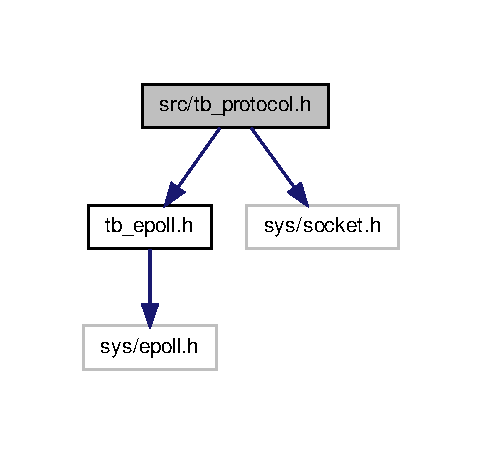
\includegraphics[width=231pt]{tb__protocol_8h__incl}
\end{center}
\end{figure}
This graph shows which files directly or indirectly include this file\-:\nopagebreak
\begin{figure}[H]
\begin{center}
\leavevmode
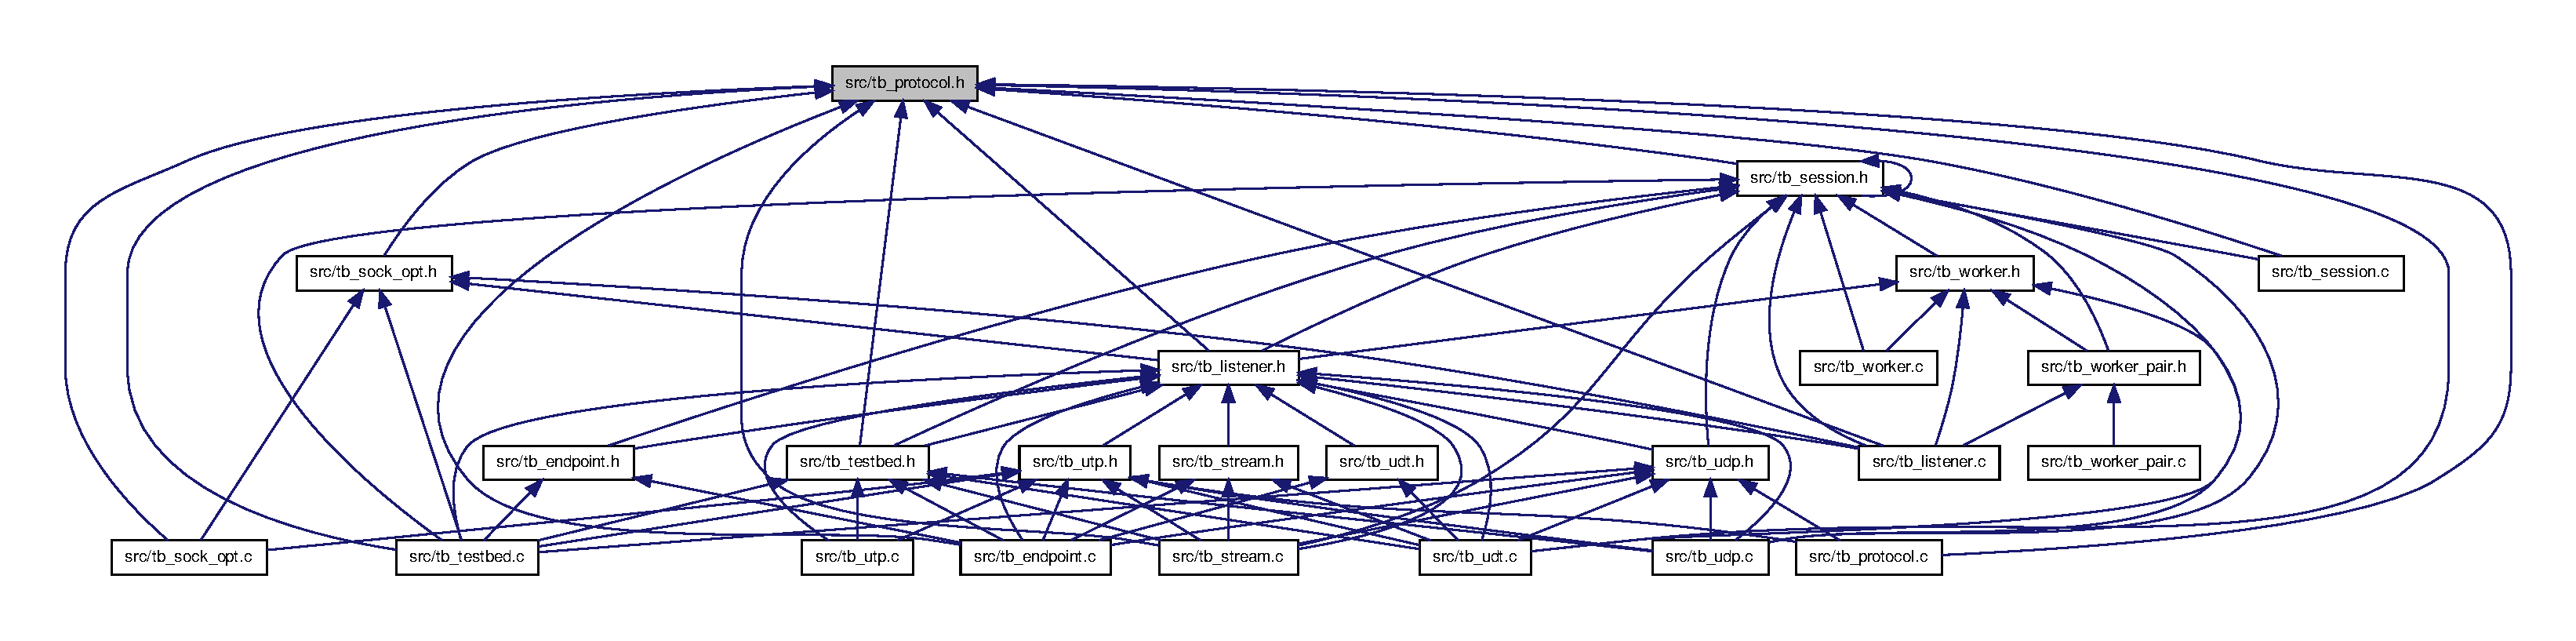
\includegraphics[width=350pt]{tb__protocol_8h__dep__incl}
\end{center}
\end{figure}
\subsection*{Data Structures}
\begin{DoxyCompactItemize}
\item 
struct \hyperlink{structtb__protocol__t}{tb\-\_\-protocol\-\_\-t}
\begin{DoxyCompactList}\small\item\em Defines the A\-P\-I for the chosen protocol. \end{DoxyCompactList}\item 
struct \hyperlink{structtb__prot__stats__t}{tb\-\_\-prot\-\_\-stats\-\_\-t}
\begin{DoxyCompactList}\small\item\em Protocol information struct. \end{DoxyCompactList}\end{DoxyCompactItemize}
\subsection*{Typedefs}
\begin{DoxyCompactItemize}
\item 
typedef int($\ast$ \hyperlink{tb__protocol_8h_aaf09f0db257e10041fe9e53585cf883d}{funct\-\_\-socket} )(int domain, int type, int protocol)
\item 
typedef int($\ast$ \hyperlink{tb__protocol_8h_a08f2cf29907c58b40e7d04078252af61}{funct\-\_\-close} )(int fd)
\item 
typedef int($\ast$ \hyperlink{tb__protocol_8h_a14bfec37c8822819a01fb2e7f670096d}{funct\-\_\-bind} )(int fd, const struct sockaddr $\ast$addr, socklen\-\_\-t len)
\item 
typedef int($\ast$ \hyperlink{tb__protocol_8h_a43255c3ce51eb275006d03290ea299d3}{funct\-\_\-connect} )(int fd, const struct sockaddr $\ast$addr, socklen\-\_\-t len)
\item 
typedef int($\ast$ \hyperlink{tb__protocol_8h_a473a931a3082ddc4d122f9f4a8fd1437}{funct\-\_\-send} )(int fd, void $\ast$buf, size\-\_\-t n, int sock\-\_\-flags)
\item 
typedef int($\ast$ \hyperlink{tb__protocol_8h_a167282378503a61350e0d2fb4e317bb0}{funct\-\_\-recv} )(int fd, void $\ast$buf, size\-\_\-t n, int sock\-\_\-flags)
\item 
typedef int($\ast$ \hyperlink{tb__protocol_8h_aafdc81e719bafbf5836af0764e063c6e}{funct\-\_\-listen} )(int fd, int n)
\item 
typedef int($\ast$ \hyperlink{tb__protocol_8h_a35f8591b684f7643ff28a012c71b98fa}{funct\-\_\-accept} )(int fd, const struct sockaddr $\ast$addr, socklen\-\_\-t $\ast$len)
\item 
typedef int($\ast$ \hyperlink{tb__protocol_8h_ae60ccd51019fbfaaa90a036fc14349a7}{funct\-\_\-sendto} )(int fd, const void $\ast$buf, size\-\_\-t len, int flags, const struct sockaddr $\ast$dest\-\_\-addr, socklen\-\_\-t addrlen)
\item 
typedef int($\ast$ \hyperlink{tb__protocol_8h_a87e94687c2c2703bd383b95da63fadfb}{funct\-\_\-recvfrom} )(int fd, void $\ast$buf, int len, unsigned int flags, const struct sockaddr $\ast$to, socklen\-\_\-t $\ast$tolen)
\item 
typedef void($\ast$ \hyperlink{tb__protocol_8h_ac8027011503a44781c2e957843accec6}{funct\-\_\-exit} )()
\item 
typedef int($\ast$ \hyperlink{tb__protocol_8h_a1375c398cc002ef578b1ccef351761ef}{funct\-\_\-error} )(int value, int err\-\_\-no)
\item 
typedef int($\ast$ \hyperlink{tb__protocol_8h_a329bd89568b70a3a25d5e809f31ebac7}{funct\-\_\-options} )(int sock, int level, int optname, void $\ast$optval, int optlen)
\item 
typedef int($\ast$ \hyperlink{tb__protocol_8h_a374dd8150f3cc4a07fe29de3ec5e886a}{funct\-\_\-setup} )(void $\ast$data)
\end{DoxyCompactItemize}
\subsection*{Enumerations}
\begin{DoxyCompactItemize}
\item 
enum \hyperlink{tb__protocol_8h_a7a5bff1040fc154c510874327d44cc1a}{P\-R\-O\-T\-O\-C\-O\-L} \{ \\*
\hyperlink{tb__protocol_8h_a7a5bff1040fc154c510874327d44cc1aaa040cd7feeb588104634cdadf35abf1c}{T\-C\-P} =  0, 
\hyperlink{tb__protocol_8h_a7a5bff1040fc154c510874327d44cc1aadb542475cf9d0636e4225e216cee9ae6}{U\-D\-P} =  1, 
\hyperlink{tb__protocol_8h_a7a5bff1040fc154c510874327d44cc1aac3e38f67233c07aa15654a69175667a1}{U\-D\-T} =  2, 
\hyperlink{tb__protocol_8h_a7a5bff1040fc154c510874327d44cc1aa57a9affc769200f5e7f32843116e5dee}{a\-U\-D\-T} =  3, 
\\*
\hyperlink{tb__protocol_8h_a7a5bff1040fc154c510874327d44cc1aad637e87afa114626cf340f412dd360c1}{u\-T\-P} =  4, 
\hyperlink{tb__protocol_8h_a7a5bff1040fc154c510874327d44cc1aac93db0ed3c9fc6918df30aa4c6c994b1}{e\-U\-D\-P} =  5, 
\hyperlink{tb__protocol_8h_a7a5bff1040fc154c510874327d44cc1aa53de17981d3224badb4ed817cb3992e5}{D\-C\-C\-P} =  6
 \}
\item 
enum \hyperlink{tb__protocol_8h_ac5355051296d54a114b8691ccfc4010c}{C\-O\-N\-G\-E\-S\-T\-I\-O\-N\-\_\-\-C\-O\-N\-T\-R\-O\-L} \{ \\*
\hyperlink{tb__protocol_8h_ac5355051296d54a114b8691ccfc4010ca070d5a9959e9c4a6bfc7c75d7ab9ca98}{T\-C\-P\-\_\-\-V\-E\-G\-A\-S} =  1, 
\hyperlink{tb__protocol_8h_ac5355051296d54a114b8691ccfc4010ca9e81700deed7bc1976e1c5f84979200c}{T\-C\-P\-\_\-\-C\-U\-B\-I\-C}, 
\hyperlink{tb__protocol_8h_ac5355051296d54a114b8691ccfc4010ca95e5d0b471b6fe3b6b5403b963ed77b6}{U\-D\-T\-\_\-\-D\-A\-I\-M\-I\-D}, 
\hyperlink{tb__protocol_8h_ac5355051296d54a114b8691ccfc4010ca9d3a57c086a4a19d7094da9f1d225c26}{U\-D\-T\-\_\-\-A\-D\-A\-P\-T\-I\-V\-E}, 
\\*
\hyperlink{tb__protocol_8h_ac5355051296d54a114b8691ccfc4010ca3f8847be0dc3cb36ca1ea363b5545699}{U\-D\-P\-\_\-\-N\-O\-N\-E}
 \}
\item 
enum \hyperlink{tb__protocol_8h_ade248d634a0f3c9eca499d6fb268ce09}{P\-R\-O\-T\-\_\-\-O\-P\-T} \{ \hyperlink{tb__protocol_8h_ade248d634a0f3c9eca499d6fb268ce09aab7a8f5084a55fefe73a824f2a97e84b}{U\-S\-E\-\_\-\-B\-L\-O\-C\-K\-I\-N\-G}, 
\hyperlink{tb__protocol_8h_ade248d634a0f3c9eca499d6fb268ce09ad6b573a686274bb34934f060647fe8d9}{U\-S\-E\-\_\-\-E\-P\-O\-L\-L}
 \}
\end{DoxyCompactItemize}
\subsection*{Functions}
\begin{DoxyCompactItemize}
\item 
void \hyperlink{tb__protocol_8h_aebf261998277b8c36c9b827a3cb2f69a}{tb\-\_\-destroy\-\_\-stats} (\hyperlink{structtb__prot__stats__t}{tb\-\_\-prot\-\_\-stats\-\_\-t} $\ast$stats)
\begin{DoxyCompactList}\small\item\em Destroy stats struct. \end{DoxyCompactList}\item 
int \hyperlink{tb__protocol_8h_a634f0d467979a16f779333c4f00f97cf}{tb\-\_\-udt\-\_\-error} (int value, int err\-\_\-no)
\begin{DoxyCompactList}\small\item\em Handle errors for udt. \end{DoxyCompactList}\item 
int \hyperlink{tb__protocol_8h_a773702577cc5960a28390c6d2c637679}{tb\-\_\-dccp\-\_\-error} (int value, int err\-\_\-no)
\begin{DoxyCompactList}\small\item\em Handle errors for dccp. \end{DoxyCompactList}\item 
int \hyperlink{tb__protocol_8h_aabab4d45d896ccb2520e32d2da0a0844}{tb\-\_\-socket\-\_\-error} (int value, int err\-\_\-no)
\begin{DoxyCompactList}\small\item\em Handle errors for socket. \end{DoxyCompactList}\item 
void \hyperlink{tb__protocol_8h_a5f8e49b8ee3a8b874dd58231dd099de1}{tb\-\_\-get\-\_\-stats} (\hyperlink{structtb__prot__stats__t}{tb\-\_\-prot\-\_\-stats\-\_\-t} $\ast$stats, int fd)
\begin{DoxyCompactList}\small\item\em Get the stats for the given protocol, with the given descriptor. \end{DoxyCompactList}\item 
void \hyperlink{tb__protocol_8h_a8e38a6ede656010fb440c895610a5d10}{get\-\_\-udt\-\_\-stats} (\hyperlink{structtb__prot__stats__t}{tb\-\_\-prot\-\_\-stats\-\_\-t} $\ast$stats, int fd)
\begin{DoxyCompactList}\small\item\em Get udt stats. \end{DoxyCompactList}\item 
void \hyperlink{tb__protocol_8h_ad16e59fe4e10eb09b2aa2d190baab34e}{get\-\_\-dccp\-\_\-stats} (\hyperlink{structtb__prot__stats__t}{tb\-\_\-prot\-\_\-stats\-\_\-t} $\ast$stats, int fd)
\begin{DoxyCompactList}\small\item\em Get dccp stats. \end{DoxyCompactList}\item 
void \hyperlink{tb__protocol_8h_a8f184a229468afe5ccaa51621032fea5}{get\-\_\-tcp\-\_\-stats} (\hyperlink{structtb__prot__stats__t}{tb\-\_\-prot\-\_\-stats\-\_\-t} $\ast$stats, int fd)
\begin{DoxyCompactList}\small\item\em Get tcp stats. \end{DoxyCompactList}\item 
void \hyperlink{tb__protocol_8h_a70096149add47bfaceb6a1c893a9dfd1}{get\-\_\-udp\-\_\-stats} (\hyperlink{structtb__prot__stats__t}{tb\-\_\-prot\-\_\-stats\-\_\-t} $\ast$stats, int fd)
\begin{DoxyCompactList}\small\item\em Get udp stats. \end{DoxyCompactList}\item 
void \hyperlink{tb__protocol_8h_ae303c4e113a72eb8daf629260f13c5a3}{get\-\_\-utp\-\_\-stats} (\hyperlink{structtb__prot__stats__t}{tb\-\_\-prot\-\_\-stats\-\_\-t} $\ast$stats, int fd)
\begin{DoxyCompactList}\small\item\em Get utp stats. \end{DoxyCompactList}\item 
void \hyperlink{tb__protocol_8h_a94412470e6630d5350bf784a827034c8}{tb\-\_\-get\-\_\-bsd\-\_\-stats} (\hyperlink{structtb__prot__stats__t}{tb\-\_\-prot\-\_\-stats\-\_\-t} $\ast$stats, int fd)
\begin{DoxyCompactList}\small\item\em Get generic bsd stats. \end{DoxyCompactList}\item 
\hyperlink{structtb__protocol__t}{tb\-\_\-protocol\-\_\-t} $\ast$ \hyperlink{tb__protocol_8h_aa906a171c2fff5aaf32df7b087153ea0}{tb\-\_\-create\-\_\-protocol} (\hyperlink{tb__protocol_8h_a7a5bff1040fc154c510874327d44cc1a}{P\-R\-O\-T\-O\-C\-O\-L} prot)
\begin{DoxyCompactList}\small\item\em Create a new Protocol. \end{DoxyCompactList}\item 
void \hyperlink{tb__protocol_8h_a151f709ceb08d76f790638d9f2c55f37}{tb\-\_\-destroy\-\_\-protocol} (\hyperlink{structtb__protocol__t}{tb\-\_\-protocol\-\_\-t} $\ast$protocol)
\begin{DoxyCompactList}\small\item\em Destroy the given protocol structure. \end{DoxyCompactList}\item 
void \hyperlink{tb__protocol_8h_aa2b5480d4df920972d7dec20c54ddfe9}{tb\-\_\-print\-\_\-protocol} (\hyperlink{structtb__protocol__t}{tb\-\_\-protocol\-\_\-t} $\ast$protocol)
\begin{DoxyCompactList}\small\item\em Print the values for this protocol. \end{DoxyCompactList}\end{DoxyCompactItemize}


\subsection{Typedef Documentation}
\hypertarget{tb__protocol_8h_a35f8591b684f7643ff28a012c71b98fa}{\index{tb\-\_\-protocol.\-h@{tb\-\_\-protocol.\-h}!funct\-\_\-accept@{funct\-\_\-accept}}
\index{funct\-\_\-accept@{funct\-\_\-accept}!tb_protocol.h@{tb\-\_\-protocol.\-h}}
\subsubsection[{funct\-\_\-accept}]{\setlength{\rightskip}{0pt plus 5cm}typedef int($\ast$ funct\-\_\-accept)(int fd, const struct sockaddr $\ast$addr, socklen\-\_\-t $\ast$len)}}\label{tb__protocol_8h_a35f8591b684f7643ff28a012c71b98fa}


Definition at line 107 of file tb\-\_\-protocol.\-h.

\hypertarget{tb__protocol_8h_a14bfec37c8822819a01fb2e7f670096d}{\index{tb\-\_\-protocol.\-h@{tb\-\_\-protocol.\-h}!funct\-\_\-bind@{funct\-\_\-bind}}
\index{funct\-\_\-bind@{funct\-\_\-bind}!tb_protocol.h@{tb\-\_\-protocol.\-h}}
\subsubsection[{funct\-\_\-bind}]{\setlength{\rightskip}{0pt plus 5cm}typedef int($\ast$ funct\-\_\-bind)(int fd, const struct sockaddr $\ast$addr, socklen\-\_\-t len)}}\label{tb__protocol_8h_a14bfec37c8822819a01fb2e7f670096d}


Definition at line 77 of file tb\-\_\-protocol.\-h.

\hypertarget{tb__protocol_8h_a08f2cf29907c58b40e7d04078252af61}{\index{tb\-\_\-protocol.\-h@{tb\-\_\-protocol.\-h}!funct\-\_\-close@{funct\-\_\-close}}
\index{funct\-\_\-close@{funct\-\_\-close}!tb_protocol.h@{tb\-\_\-protocol.\-h}}
\subsubsection[{funct\-\_\-close}]{\setlength{\rightskip}{0pt plus 5cm}typedef int($\ast$ funct\-\_\-close)(int fd)}}\label{tb__protocol_8h_a08f2cf29907c58b40e7d04078252af61}


Definition at line 71 of file tb\-\_\-protocol.\-h.

\hypertarget{tb__protocol_8h_a43255c3ce51eb275006d03290ea299d3}{\index{tb\-\_\-protocol.\-h@{tb\-\_\-protocol.\-h}!funct\-\_\-connect@{funct\-\_\-connect}}
\index{funct\-\_\-connect@{funct\-\_\-connect}!tb_protocol.h@{tb\-\_\-protocol.\-h}}
\subsubsection[{funct\-\_\-connect}]{\setlength{\rightskip}{0pt plus 5cm}typedef int($\ast$ funct\-\_\-connect)(int fd, const struct sockaddr $\ast$addr, socklen\-\_\-t len)}}\label{tb__protocol_8h_a43255c3ce51eb275006d03290ea299d3}


Definition at line 83 of file tb\-\_\-protocol.\-h.

\hypertarget{tb__protocol_8h_a1375c398cc002ef578b1ccef351761ef}{\index{tb\-\_\-protocol.\-h@{tb\-\_\-protocol.\-h}!funct\-\_\-error@{funct\-\_\-error}}
\index{funct\-\_\-error@{funct\-\_\-error}!tb_protocol.h@{tb\-\_\-protocol.\-h}}
\subsubsection[{funct\-\_\-error}]{\setlength{\rightskip}{0pt plus 5cm}typedef int($\ast$ funct\-\_\-error)(int value, int err\-\_\-no)}}\label{tb__protocol_8h_a1375c398cc002ef578b1ccef351761ef}


Definition at line 133 of file tb\-\_\-protocol.\-h.

\hypertarget{tb__protocol_8h_ac8027011503a44781c2e957843accec6}{\index{tb\-\_\-protocol.\-h@{tb\-\_\-protocol.\-h}!funct\-\_\-exit@{funct\-\_\-exit}}
\index{funct\-\_\-exit@{funct\-\_\-exit}!tb_protocol.h@{tb\-\_\-protocol.\-h}}
\subsubsection[{funct\-\_\-exit}]{\setlength{\rightskip}{0pt plus 5cm}typedef void($\ast$ funct\-\_\-exit)()}}\label{tb__protocol_8h_ac8027011503a44781c2e957843accec6}


Definition at line 127 of file tb\-\_\-protocol.\-h.

\hypertarget{tb__protocol_8h_aafdc81e719bafbf5836af0764e063c6e}{\index{tb\-\_\-protocol.\-h@{tb\-\_\-protocol.\-h}!funct\-\_\-listen@{funct\-\_\-listen}}
\index{funct\-\_\-listen@{funct\-\_\-listen}!tb_protocol.h@{tb\-\_\-protocol.\-h}}
\subsubsection[{funct\-\_\-listen}]{\setlength{\rightskip}{0pt plus 5cm}typedef int($\ast$ funct\-\_\-listen)(int fd, int n)}}\label{tb__protocol_8h_aafdc81e719bafbf5836af0764e063c6e}


Definition at line 101 of file tb\-\_\-protocol.\-h.

\hypertarget{tb__protocol_8h_a329bd89568b70a3a25d5e809f31ebac7}{\index{tb\-\_\-protocol.\-h@{tb\-\_\-protocol.\-h}!funct\-\_\-options@{funct\-\_\-options}}
\index{funct\-\_\-options@{funct\-\_\-options}!tb_protocol.h@{tb\-\_\-protocol.\-h}}
\subsubsection[{funct\-\_\-options}]{\setlength{\rightskip}{0pt plus 5cm}typedef int($\ast$ funct\-\_\-options)(int sock, int level, int optname, void $\ast$optval, int optlen)}}\label{tb__protocol_8h_a329bd89568b70a3a25d5e809f31ebac7}


Definition at line 139 of file tb\-\_\-protocol.\-h.

\hypertarget{tb__protocol_8h_a167282378503a61350e0d2fb4e317bb0}{\index{tb\-\_\-protocol.\-h@{tb\-\_\-protocol.\-h}!funct\-\_\-recv@{funct\-\_\-recv}}
\index{funct\-\_\-recv@{funct\-\_\-recv}!tb_protocol.h@{tb\-\_\-protocol.\-h}}
\subsubsection[{funct\-\_\-recv}]{\setlength{\rightskip}{0pt plus 5cm}typedef int($\ast$ funct\-\_\-recv)(int fd, void $\ast$buf, size\-\_\-t n, int sock\-\_\-flags)}}\label{tb__protocol_8h_a167282378503a61350e0d2fb4e317bb0}


Definition at line 95 of file tb\-\_\-protocol.\-h.

\hypertarget{tb__protocol_8h_a87e94687c2c2703bd383b95da63fadfb}{\index{tb\-\_\-protocol.\-h@{tb\-\_\-protocol.\-h}!funct\-\_\-recvfrom@{funct\-\_\-recvfrom}}
\index{funct\-\_\-recvfrom@{funct\-\_\-recvfrom}!tb_protocol.h@{tb\-\_\-protocol.\-h}}
\subsubsection[{funct\-\_\-recvfrom}]{\setlength{\rightskip}{0pt plus 5cm}typedef int($\ast$ funct\-\_\-recvfrom)(int fd, void $\ast$buf, int len, unsigned int flags, const struct sockaddr $\ast$to, socklen\-\_\-t $\ast$tolen)}}\label{tb__protocol_8h_a87e94687c2c2703bd383b95da63fadfb}


Definition at line 120 of file tb\-\_\-protocol.\-h.

\hypertarget{tb__protocol_8h_a473a931a3082ddc4d122f9f4a8fd1437}{\index{tb\-\_\-protocol.\-h@{tb\-\_\-protocol.\-h}!funct\-\_\-send@{funct\-\_\-send}}
\index{funct\-\_\-send@{funct\-\_\-send}!tb_protocol.h@{tb\-\_\-protocol.\-h}}
\subsubsection[{funct\-\_\-send}]{\setlength{\rightskip}{0pt plus 5cm}typedef int($\ast$ funct\-\_\-send)(int fd, void $\ast$buf, size\-\_\-t n, int sock\-\_\-flags)}}\label{tb__protocol_8h_a473a931a3082ddc4d122f9f4a8fd1437}


Definition at line 89 of file tb\-\_\-protocol.\-h.

\hypertarget{tb__protocol_8h_ae60ccd51019fbfaaa90a036fc14349a7}{\index{tb\-\_\-protocol.\-h@{tb\-\_\-protocol.\-h}!funct\-\_\-sendto@{funct\-\_\-sendto}}
\index{funct\-\_\-sendto@{funct\-\_\-sendto}!tb_protocol.h@{tb\-\_\-protocol.\-h}}
\subsubsection[{funct\-\_\-sendto}]{\setlength{\rightskip}{0pt plus 5cm}typedef int($\ast$ funct\-\_\-sendto)(int fd, const void $\ast$buf, size\-\_\-t len, int flags, const struct sockaddr $\ast$dest\-\_\-addr, socklen\-\_\-t addrlen)}}\label{tb__protocol_8h_ae60ccd51019fbfaaa90a036fc14349a7}


Definition at line 113 of file tb\-\_\-protocol.\-h.

\hypertarget{tb__protocol_8h_a374dd8150f3cc4a07fe29de3ec5e886a}{\index{tb\-\_\-protocol.\-h@{tb\-\_\-protocol.\-h}!funct\-\_\-setup@{funct\-\_\-setup}}
\index{funct\-\_\-setup@{funct\-\_\-setup}!tb_protocol.h@{tb\-\_\-protocol.\-h}}
\subsubsection[{funct\-\_\-setup}]{\setlength{\rightskip}{0pt plus 5cm}typedef int($\ast$ funct\-\_\-setup)(void $\ast$data)}}\label{tb__protocol_8h_a374dd8150f3cc4a07fe29de3ec5e886a}


Definition at line 146 of file tb\-\_\-protocol.\-h.

\hypertarget{tb__protocol_8h_aaf09f0db257e10041fe9e53585cf883d}{\index{tb\-\_\-protocol.\-h@{tb\-\_\-protocol.\-h}!funct\-\_\-socket@{funct\-\_\-socket}}
\index{funct\-\_\-socket@{funct\-\_\-socket}!tb_protocol.h@{tb\-\_\-protocol.\-h}}
\subsubsection[{funct\-\_\-socket}]{\setlength{\rightskip}{0pt plus 5cm}typedef int($\ast$ funct\-\_\-socket)(int domain, int type, int protocol)}}\label{tb__protocol_8h_aaf09f0db257e10041fe9e53585cf883d}


Definition at line 65 of file tb\-\_\-protocol.\-h.



\subsection{Enumeration Type Documentation}
\hypertarget{tb__protocol_8h_ac5355051296d54a114b8691ccfc4010c}{\index{tb\-\_\-protocol.\-h@{tb\-\_\-protocol.\-h}!C\-O\-N\-G\-E\-S\-T\-I\-O\-N\-\_\-\-C\-O\-N\-T\-R\-O\-L@{C\-O\-N\-G\-E\-S\-T\-I\-O\-N\-\_\-\-C\-O\-N\-T\-R\-O\-L}}
\index{C\-O\-N\-G\-E\-S\-T\-I\-O\-N\-\_\-\-C\-O\-N\-T\-R\-O\-L@{C\-O\-N\-G\-E\-S\-T\-I\-O\-N\-\_\-\-C\-O\-N\-T\-R\-O\-L}!tb_protocol.h@{tb\-\_\-protocol.\-h}}
\subsubsection[{C\-O\-N\-G\-E\-S\-T\-I\-O\-N\-\_\-\-C\-O\-N\-T\-R\-O\-L}]{\setlength{\rightskip}{0pt plus 5cm}enum {\bf C\-O\-N\-G\-E\-S\-T\-I\-O\-N\-\_\-\-C\-O\-N\-T\-R\-O\-L}}}\label{tb__protocol_8h_ac5355051296d54a114b8691ccfc4010c}
\begin{Desc}
\item[Enumerator\-: ]\par
\begin{description}
\index{T\-C\-P\-\_\-\-V\-E\-G\-A\-S@{T\-C\-P\-\_\-\-V\-E\-G\-A\-S}!tb\-\_\-protocol.\-h@{tb\-\_\-protocol.\-h}}\index{tb\-\_\-protocol.\-h@{tb\-\_\-protocol.\-h}!T\-C\-P\-\_\-\-V\-E\-G\-A\-S@{T\-C\-P\-\_\-\-V\-E\-G\-A\-S}}\item[{\em 
\hypertarget{tb__protocol_8h_ac5355051296d54a114b8691ccfc4010ca070d5a9959e9c4a6bfc7c75d7ab9ca98}{T\-C\-P\-\_\-\-V\-E\-G\-A\-S}\label{tb__protocol_8h_ac5355051296d54a114b8691ccfc4010ca070d5a9959e9c4a6bfc7c75d7ab9ca98}
}]The T\-C\-P vegas control algorithm. \index{T\-C\-P\-\_\-\-C\-U\-B\-I\-C@{T\-C\-P\-\_\-\-C\-U\-B\-I\-C}!tb\-\_\-protocol.\-h@{tb\-\_\-protocol.\-h}}\index{tb\-\_\-protocol.\-h@{tb\-\_\-protocol.\-h}!T\-C\-P\-\_\-\-C\-U\-B\-I\-C@{T\-C\-P\-\_\-\-C\-U\-B\-I\-C}}\item[{\em 
\hypertarget{tb__protocol_8h_ac5355051296d54a114b8691ccfc4010ca9e81700deed7bc1976e1c5f84979200c}{T\-C\-P\-\_\-\-C\-U\-B\-I\-C}\label{tb__protocol_8h_ac5355051296d54a114b8691ccfc4010ca9e81700deed7bc1976e1c5f84979200c}
}]The T\-C\-P C\-U\-B\-I\-C control algorithm. \index{U\-D\-T\-\_\-\-D\-A\-I\-M\-I\-D@{U\-D\-T\-\_\-\-D\-A\-I\-M\-I\-D}!tb\-\_\-protocol.\-h@{tb\-\_\-protocol.\-h}}\index{tb\-\_\-protocol.\-h@{tb\-\_\-protocol.\-h}!U\-D\-T\-\_\-\-D\-A\-I\-M\-I\-D@{U\-D\-T\-\_\-\-D\-A\-I\-M\-I\-D}}\item[{\em 
\hypertarget{tb__protocol_8h_ac5355051296d54a114b8691ccfc4010ca95e5d0b471b6fe3b6b5403b963ed77b6}{U\-D\-T\-\_\-\-D\-A\-I\-M\-I\-D}\label{tb__protocol_8h_ac5355051296d54a114b8691ccfc4010ca95e5d0b471b6fe3b6b5403b963ed77b6}
}]U\-D\-T's default control algorithm. \index{U\-D\-T\-\_\-\-A\-D\-A\-P\-T\-I\-V\-E@{U\-D\-T\-\_\-\-A\-D\-A\-P\-T\-I\-V\-E}!tb\-\_\-protocol.\-h@{tb\-\_\-protocol.\-h}}\index{tb\-\_\-protocol.\-h@{tb\-\_\-protocol.\-h}!U\-D\-T\-\_\-\-A\-D\-A\-P\-T\-I\-V\-E@{U\-D\-T\-\_\-\-A\-D\-A\-P\-T\-I\-V\-E}}\item[{\em 
\hypertarget{tb__protocol_8h_ac5355051296d54a114b8691ccfc4010ca9d3a57c086a4a19d7094da9f1d225c26}{U\-D\-T\-\_\-\-A\-D\-A\-P\-T\-I\-V\-E}\label{tb__protocol_8h_ac5355051296d54a114b8691ccfc4010ca9d3a57c086a4a19d7094da9f1d225c26}
}]The new algorithm added to U\-D\-T. \index{U\-D\-P\-\_\-\-N\-O\-N\-E@{U\-D\-P\-\_\-\-N\-O\-N\-E}!tb\-\_\-protocol.\-h@{tb\-\_\-protocol.\-h}}\index{tb\-\_\-protocol.\-h@{tb\-\_\-protocol.\-h}!U\-D\-P\-\_\-\-N\-O\-N\-E@{U\-D\-P\-\_\-\-N\-O\-N\-E}}\item[{\em 
\hypertarget{tb__protocol_8h_ac5355051296d54a114b8691ccfc4010ca3f8847be0dc3cb36ca1ea363b5545699}{U\-D\-P\-\_\-\-N\-O\-N\-E}\label{tb__protocol_8h_ac5355051296d54a114b8691ccfc4010ca3f8847be0dc3cb36ca1ea363b5545699}
}]U\-D\-P does not use congestion control. \end{description}
\end{Desc}



Definition at line 39 of file tb\-\_\-protocol.\-h.

\hypertarget{tb__protocol_8h_ade248d634a0f3c9eca499d6fb268ce09}{\index{tb\-\_\-protocol.\-h@{tb\-\_\-protocol.\-h}!P\-R\-O\-T\-\_\-\-O\-P\-T@{P\-R\-O\-T\-\_\-\-O\-P\-T}}
\index{P\-R\-O\-T\-\_\-\-O\-P\-T@{P\-R\-O\-T\-\_\-\-O\-P\-T}!tb_protocol.h@{tb\-\_\-protocol.\-h}}
\subsubsection[{P\-R\-O\-T\-\_\-\-O\-P\-T}]{\setlength{\rightskip}{0pt plus 5cm}enum {\bf P\-R\-O\-T\-\_\-\-O\-P\-T}}}\label{tb__protocol_8h_ade248d634a0f3c9eca499d6fb268ce09}
\begin{Desc}
\item[Enumerator\-: ]\par
\begin{description}
\index{U\-S\-E\-\_\-\-B\-L\-O\-C\-K\-I\-N\-G@{U\-S\-E\-\_\-\-B\-L\-O\-C\-K\-I\-N\-G}!tb\-\_\-protocol.\-h@{tb\-\_\-protocol.\-h}}\index{tb\-\_\-protocol.\-h@{tb\-\_\-protocol.\-h}!U\-S\-E\-\_\-\-B\-L\-O\-C\-K\-I\-N\-G@{U\-S\-E\-\_\-\-B\-L\-O\-C\-K\-I\-N\-G}}\item[{\em 
\hypertarget{tb__protocol_8h_ade248d634a0f3c9eca499d6fb268ce09aab7a8f5084a55fefe73a824f2a97e84b}{U\-S\-E\-\_\-\-B\-L\-O\-C\-K\-I\-N\-G}\label{tb__protocol_8h_ade248d634a0f3c9eca499d6fb268ce09aab7a8f5084a55fefe73a824f2a97e84b}
}]Use standard blocking sockets. \index{U\-S\-E\-\_\-\-E\-P\-O\-L\-L@{U\-S\-E\-\_\-\-E\-P\-O\-L\-L}!tb\-\_\-protocol.\-h@{tb\-\_\-protocol.\-h}}\index{tb\-\_\-protocol.\-h@{tb\-\_\-protocol.\-h}!U\-S\-E\-\_\-\-E\-P\-O\-L\-L@{U\-S\-E\-\_\-\-E\-P\-O\-L\-L}}\item[{\em 
\hypertarget{tb__protocol_8h_ade248d634a0f3c9eca499d6fb268ce09ad6b573a686274bb34934f060647fe8d9}{U\-S\-E\-\_\-\-E\-P\-O\-L\-L}\label{tb__protocol_8h_ade248d634a0f3c9eca499d6fb268ce09ad6b573a686274bb34934f060647fe8d9}
}]Use Epoll for sockets. \end{description}
\end{Desc}



Definition at line 54 of file tb\-\_\-protocol.\-h.

\hypertarget{tb__protocol_8h_a7a5bff1040fc154c510874327d44cc1a}{\index{tb\-\_\-protocol.\-h@{tb\-\_\-protocol.\-h}!P\-R\-O\-T\-O\-C\-O\-L@{P\-R\-O\-T\-O\-C\-O\-L}}
\index{P\-R\-O\-T\-O\-C\-O\-L@{P\-R\-O\-T\-O\-C\-O\-L}!tb_protocol.h@{tb\-\_\-protocol.\-h}}
\subsubsection[{P\-R\-O\-T\-O\-C\-O\-L}]{\setlength{\rightskip}{0pt plus 5cm}enum {\bf P\-R\-O\-T\-O\-C\-O\-L}}}\label{tb__protocol_8h_a7a5bff1040fc154c510874327d44cc1a}
\begin{Desc}
\item[Enumerator\-: ]\par
\begin{description}
\index{T\-C\-P@{T\-C\-P}!tb\-\_\-protocol.\-h@{tb\-\_\-protocol.\-h}}\index{tb\-\_\-protocol.\-h@{tb\-\_\-protocol.\-h}!T\-C\-P@{T\-C\-P}}\item[{\em 
\hypertarget{tb__protocol_8h_a7a5bff1040fc154c510874327d44cc1aaa040cd7feeb588104634cdadf35abf1c}{T\-C\-P}\label{tb__protocol_8h_a7a5bff1040fc154c510874327d44cc1aaa040cd7feeb588104634cdadf35abf1c}
}]Regular, garden variety T\-C\-P. Yawn. \index{U\-D\-P@{U\-D\-P}!tb\-\_\-protocol.\-h@{tb\-\_\-protocol.\-h}}\index{tb\-\_\-protocol.\-h@{tb\-\_\-protocol.\-h}!U\-D\-P@{U\-D\-P}}\item[{\em 
\hypertarget{tb__protocol_8h_a7a5bff1040fc154c510874327d44cc1aadb542475cf9d0636e4225e216cee9ae6}{U\-D\-P}\label{tb__protocol_8h_a7a5bff1040fc154c510874327d44cc1aadb542475cf9d0636e4225e216cee9ae6}
}]Regular, garden variety U\-D\-P. \index{U\-D\-T@{U\-D\-T}!tb\-\_\-protocol.\-h@{tb\-\_\-protocol.\-h}}\index{tb\-\_\-protocol.\-h@{tb\-\_\-protocol.\-h}!U\-D\-T@{U\-D\-T}}\item[{\em 
\hypertarget{tb__protocol_8h_a7a5bff1040fc154c510874327d44cc1aac3e38f67233c07aa15654a69175667a1}{U\-D\-T}\label{tb__protocol_8h_a7a5bff1040fc154c510874327d44cc1aac3e38f67233c07aa15654a69175667a1}
}]Flash and fun U\-D\-T, please. \index{a\-U\-D\-T@{a\-U\-D\-T}!tb\-\_\-protocol.\-h@{tb\-\_\-protocol.\-h}}\index{tb\-\_\-protocol.\-h@{tb\-\_\-protocol.\-h}!a\-U\-D\-T@{a\-U\-D\-T}}\item[{\em 
\hypertarget{tb__protocol_8h_a7a5bff1040fc154c510874327d44cc1aa57a9affc769200f5e7f32843116e5dee}{a\-U\-D\-T}\label{tb__protocol_8h_a7a5bff1040fc154c510874327d44cc1aa57a9affc769200f5e7f32843116e5dee}
}]Yet to be implemented adaptive U\-D\-T. \index{u\-T\-P@{u\-T\-P}!tb\-\_\-protocol.\-h@{tb\-\_\-protocol.\-h}}\index{tb\-\_\-protocol.\-h@{tb\-\_\-protocol.\-h}!u\-T\-P@{u\-T\-P}}\item[{\em 
\hypertarget{tb__protocol_8h_a7a5bff1040fc154c510874327d44cc1aad637e87afa114626cf340f412dd360c1}{u\-T\-P}\label{tb__protocol_8h_a7a5bff1040fc154c510874327d44cc1aad637e87afa114626cf340f412dd360c1}
}]Arrrr a pirates favourite protocol. \index{e\-U\-D\-P@{e\-U\-D\-P}!tb\-\_\-protocol.\-h@{tb\-\_\-protocol.\-h}}\index{tb\-\_\-protocol.\-h@{tb\-\_\-protocol.\-h}!e\-U\-D\-P@{e\-U\-D\-P}}\item[{\em 
\hypertarget{tb__protocol_8h_a7a5bff1040fc154c510874327d44cc1aac93db0ed3c9fc6918df30aa4c6c994b1}{e\-U\-D\-P}\label{tb__protocol_8h_a7a5bff1040fc154c510874327d44cc1aac93db0ed3c9fc6918df30aa4c6c994b1}
}]U\-D\-P with epoll. \index{D\-C\-C\-P@{D\-C\-C\-P}!tb\-\_\-protocol.\-h@{tb\-\_\-protocol.\-h}}\index{tb\-\_\-protocol.\-h@{tb\-\_\-protocol.\-h}!D\-C\-C\-P@{D\-C\-C\-P}}\item[{\em 
\hypertarget{tb__protocol_8h_a7a5bff1040fc154c510874327d44cc1aa53de17981d3224badb4ed817cb3992e5}{D\-C\-C\-P}\label{tb__protocol_8h_a7a5bff1040fc154c510874327d44cc1aa53de17981d3224badb4ed817cb3992e5}
}]D\-C\-C\-P, in linux kernal. \end{description}
\end{Desc}



Definition at line 21 of file tb\-\_\-protocol.\-h.



\subsection{Function Documentation}
\hypertarget{tb__protocol_8h_ad16e59fe4e10eb09b2aa2d190baab34e}{\index{tb\-\_\-protocol.\-h@{tb\-\_\-protocol.\-h}!get\-\_\-dccp\-\_\-stats@{get\-\_\-dccp\-\_\-stats}}
\index{get\-\_\-dccp\-\_\-stats@{get\-\_\-dccp\-\_\-stats}!tb_protocol.h@{tb\-\_\-protocol.\-h}}
\subsubsection[{get\-\_\-dccp\-\_\-stats}]{\setlength{\rightskip}{0pt plus 5cm}void get\-\_\-dccp\-\_\-stats (
\begin{DoxyParamCaption}
\item[{{\bf tb\-\_\-prot\-\_\-stats\-\_\-t} $\ast$}]{stats, }
\item[{int}]{fd}
\end{DoxyParamCaption}
)}}\label{tb__protocol_8h_ad16e59fe4e10eb09b2aa2d190baab34e}


Get dccp stats. 



Definition at line 299 of file tb\-\_\-protocol.\-c.

\hypertarget{tb__protocol_8h_a8f184a229468afe5ccaa51621032fea5}{\index{tb\-\_\-protocol.\-h@{tb\-\_\-protocol.\-h}!get\-\_\-tcp\-\_\-stats@{get\-\_\-tcp\-\_\-stats}}
\index{get\-\_\-tcp\-\_\-stats@{get\-\_\-tcp\-\_\-stats}!tb_protocol.h@{tb\-\_\-protocol.\-h}}
\subsubsection[{get\-\_\-tcp\-\_\-stats}]{\setlength{\rightskip}{0pt plus 5cm}void get\-\_\-tcp\-\_\-stats (
\begin{DoxyParamCaption}
\item[{{\bf tb\-\_\-prot\-\_\-stats\-\_\-t} $\ast$}]{stats, }
\item[{int}]{fd}
\end{DoxyParamCaption}
)}}\label{tb__protocol_8h_a8f184a229468afe5ccaa51621032fea5}


Get tcp stats. 



Definition at line 305 of file tb\-\_\-protocol.\-c.

\hypertarget{tb__protocol_8h_a70096149add47bfaceb6a1c893a9dfd1}{\index{tb\-\_\-protocol.\-h@{tb\-\_\-protocol.\-h}!get\-\_\-udp\-\_\-stats@{get\-\_\-udp\-\_\-stats}}
\index{get\-\_\-udp\-\_\-stats@{get\-\_\-udp\-\_\-stats}!tb_protocol.h@{tb\-\_\-protocol.\-h}}
\subsubsection[{get\-\_\-udp\-\_\-stats}]{\setlength{\rightskip}{0pt plus 5cm}void get\-\_\-udp\-\_\-stats (
\begin{DoxyParamCaption}
\item[{{\bf tb\-\_\-prot\-\_\-stats\-\_\-t} $\ast$}]{stats, }
\item[{int}]{fd}
\end{DoxyParamCaption}
)}}\label{tb__protocol_8h_a70096149add47bfaceb6a1c893a9dfd1}


Get udp stats. 



Definition at line 287 of file tb\-\_\-protocol.\-c.

\hypertarget{tb__protocol_8h_a8e38a6ede656010fb440c895610a5d10}{\index{tb\-\_\-protocol.\-h@{tb\-\_\-protocol.\-h}!get\-\_\-udt\-\_\-stats@{get\-\_\-udt\-\_\-stats}}
\index{get\-\_\-udt\-\_\-stats@{get\-\_\-udt\-\_\-stats}!tb_protocol.h@{tb\-\_\-protocol.\-h}}
\subsubsection[{get\-\_\-udt\-\_\-stats}]{\setlength{\rightskip}{0pt plus 5cm}void get\-\_\-udt\-\_\-stats (
\begin{DoxyParamCaption}
\item[{{\bf tb\-\_\-prot\-\_\-stats\-\_\-t} $\ast$}]{stats, }
\item[{int}]{fd}
\end{DoxyParamCaption}
)}}\label{tb__protocol_8h_a8e38a6ede656010fb440c895610a5d10}


Get udt stats. 



Definition at line 258 of file tb\-\_\-protocol.\-c.

\hypertarget{tb__protocol_8h_ae303c4e113a72eb8daf629260f13c5a3}{\index{tb\-\_\-protocol.\-h@{tb\-\_\-protocol.\-h}!get\-\_\-utp\-\_\-stats@{get\-\_\-utp\-\_\-stats}}
\index{get\-\_\-utp\-\_\-stats@{get\-\_\-utp\-\_\-stats}!tb_protocol.h@{tb\-\_\-protocol.\-h}}
\subsubsection[{get\-\_\-utp\-\_\-stats}]{\setlength{\rightskip}{0pt plus 5cm}void get\-\_\-utp\-\_\-stats (
\begin{DoxyParamCaption}
\item[{{\bf tb\-\_\-prot\-\_\-stats\-\_\-t} $\ast$}]{stats, }
\item[{int}]{fd}
\end{DoxyParamCaption}
)}}\label{tb__protocol_8h_ae303c4e113a72eb8daf629260f13c5a3}


Get utp stats. 



Definition at line 293 of file tb\-\_\-protocol.\-c.

\hypertarget{tb__protocol_8h_aa906a171c2fff5aaf32df7b087153ea0}{\index{tb\-\_\-protocol.\-h@{tb\-\_\-protocol.\-h}!tb\-\_\-create\-\_\-protocol@{tb\-\_\-create\-\_\-protocol}}
\index{tb\-\_\-create\-\_\-protocol@{tb\-\_\-create\-\_\-protocol}!tb_protocol.h@{tb\-\_\-protocol.\-h}}
\subsubsection[{tb\-\_\-create\-\_\-protocol}]{\setlength{\rightskip}{0pt plus 5cm}{\bf tb\-\_\-protocol\-\_\-t}$\ast$ tb\-\_\-create\-\_\-protocol (
\begin{DoxyParamCaption}
\item[{{\bf P\-R\-O\-T\-O\-C\-O\-L}}]{prot}
\end{DoxyParamCaption}
)}}\label{tb__protocol_8h_aa906a171c2fff5aaf32df7b087153ea0}


Create a new Protocol. 

Creates the protocol, and loads the struct with all of the relevant functions to perform communication.

\begin{DoxyPrecond}{Precondition}
The protocol must be one of the supported types. 
\end{DoxyPrecond}

\begin{DoxyParams}{Parameters}
{\em prot} & The protocol to use in the tests. \\
\hline
\end{DoxyParams}
\begin{DoxyReturn}{Returns}
The struct \hyperlink{structtb__protocol__t}{tb\-\_\-protocol\-\_\-t} 
\end{DoxyReturn}


Definition at line 27 of file tb\-\_\-protocol.\-c.

\hypertarget{tb__protocol_8h_a773702577cc5960a28390c6d2c637679}{\index{tb\-\_\-protocol.\-h@{tb\-\_\-protocol.\-h}!tb\-\_\-dccp\-\_\-error@{tb\-\_\-dccp\-\_\-error}}
\index{tb\-\_\-dccp\-\_\-error@{tb\-\_\-dccp\-\_\-error}!tb_protocol.h@{tb\-\_\-protocol.\-h}}
\subsubsection[{tb\-\_\-dccp\-\_\-error}]{\setlength{\rightskip}{0pt plus 5cm}int tb\-\_\-dccp\-\_\-error (
\begin{DoxyParamCaption}
\item[{int}]{value, }
\item[{int}]{err\-\_\-no}
\end{DoxyParamCaption}
)}}\label{tb__protocol_8h_a773702577cc5960a28390c6d2c637679}


Handle errors for dccp. 



Definition at line 192 of file tb\-\_\-protocol.\-c.

\hypertarget{tb__protocol_8h_a151f709ceb08d76f790638d9f2c55f37}{\index{tb\-\_\-protocol.\-h@{tb\-\_\-protocol.\-h}!tb\-\_\-destroy\-\_\-protocol@{tb\-\_\-destroy\-\_\-protocol}}
\index{tb\-\_\-destroy\-\_\-protocol@{tb\-\_\-destroy\-\_\-protocol}!tb_protocol.h@{tb\-\_\-protocol.\-h}}
\subsubsection[{tb\-\_\-destroy\-\_\-protocol}]{\setlength{\rightskip}{0pt plus 5cm}void tb\-\_\-destroy\-\_\-protocol (
\begin{DoxyParamCaption}
\item[{{\bf tb\-\_\-protocol\-\_\-t} $\ast$}]{protocol}
\end{DoxyParamCaption}
)}}\label{tb__protocol_8h_a151f709ceb08d76f790638d9f2c55f37}


Destroy the given protocol structure. 

Destroys the struct, freeing up memory.

\begin{DoxyPrecond}{Precondition}
protocol must be of type \hyperlink{structtb__protocol__t}{tb\-\_\-protocol\-\_\-t}. 
\end{DoxyPrecond}

\begin{DoxyParams}{Parameters}
{\em protocol} & The struct to destroy. \\
\hline
\end{DoxyParams}


Definition at line 344 of file tb\-\_\-protocol.\-c.

\hypertarget{tb__protocol_8h_aebf261998277b8c36c9b827a3cb2f69a}{\index{tb\-\_\-protocol.\-h@{tb\-\_\-protocol.\-h}!tb\-\_\-destroy\-\_\-stats@{tb\-\_\-destroy\-\_\-stats}}
\index{tb\-\_\-destroy\-\_\-stats@{tb\-\_\-destroy\-\_\-stats}!tb_protocol.h@{tb\-\_\-protocol.\-h}}
\subsubsection[{tb\-\_\-destroy\-\_\-stats}]{\setlength{\rightskip}{0pt plus 5cm}void tb\-\_\-destroy\-\_\-stats (
\begin{DoxyParamCaption}
\item[{{\bf tb\-\_\-prot\-\_\-stats\-\_\-t} $\ast$}]{stats}
\end{DoxyParamCaption}
)}}\label{tb__protocol_8h_aebf261998277b8c36c9b827a3cb2f69a}


Destroy stats struct. 



Definition at line 247 of file tb\-\_\-protocol.\-c.

\hypertarget{tb__protocol_8h_a94412470e6630d5350bf784a827034c8}{\index{tb\-\_\-protocol.\-h@{tb\-\_\-protocol.\-h}!tb\-\_\-get\-\_\-bsd\-\_\-stats@{tb\-\_\-get\-\_\-bsd\-\_\-stats}}
\index{tb\-\_\-get\-\_\-bsd\-\_\-stats@{tb\-\_\-get\-\_\-bsd\-\_\-stats}!tb_protocol.h@{tb\-\_\-protocol.\-h}}
\subsubsection[{tb\-\_\-get\-\_\-bsd\-\_\-stats}]{\setlength{\rightskip}{0pt plus 5cm}void tb\-\_\-get\-\_\-bsd\-\_\-stats (
\begin{DoxyParamCaption}
\item[{{\bf tb\-\_\-prot\-\_\-stats\-\_\-t} $\ast$}]{stats, }
\item[{int}]{fd}
\end{DoxyParamCaption}
)}}\label{tb__protocol_8h_a94412470e6630d5350bf784a827034c8}


Get generic bsd stats. 



Definition at line 334 of file tb\-\_\-protocol.\-c.

\hypertarget{tb__protocol_8h_a5f8e49b8ee3a8b874dd58231dd099de1}{\index{tb\-\_\-protocol.\-h@{tb\-\_\-protocol.\-h}!tb\-\_\-get\-\_\-stats@{tb\-\_\-get\-\_\-stats}}
\index{tb\-\_\-get\-\_\-stats@{tb\-\_\-get\-\_\-stats}!tb_protocol.h@{tb\-\_\-protocol.\-h}}
\subsubsection[{tb\-\_\-get\-\_\-stats}]{\setlength{\rightskip}{0pt plus 5cm}void tb\-\_\-get\-\_\-stats (
\begin{DoxyParamCaption}
\item[{{\bf tb\-\_\-prot\-\_\-stats\-\_\-t} $\ast$}]{stats, }
\item[{int}]{fd}
\end{DoxyParamCaption}
)}}\label{tb__protocol_8h_a5f8e49b8ee3a8b874dd58231dd099de1}


Get the stats for the given protocol, with the given descriptor. 



Definition at line 215 of file tb\-\_\-protocol.\-c.

\hypertarget{tb__protocol_8h_aa2b5480d4df920972d7dec20c54ddfe9}{\index{tb\-\_\-protocol.\-h@{tb\-\_\-protocol.\-h}!tb\-\_\-print\-\_\-protocol@{tb\-\_\-print\-\_\-protocol}}
\index{tb\-\_\-print\-\_\-protocol@{tb\-\_\-print\-\_\-protocol}!tb_protocol.h@{tb\-\_\-protocol.\-h}}
\subsubsection[{tb\-\_\-print\-\_\-protocol}]{\setlength{\rightskip}{0pt plus 5cm}void tb\-\_\-print\-\_\-protocol (
\begin{DoxyParamCaption}
\item[{{\bf tb\-\_\-protocol\-\_\-t} $\ast$}]{protocol}
\end{DoxyParamCaption}
)}}\label{tb__protocol_8h_aa2b5480d4df920972d7dec20c54ddfe9}


Print the values for this protocol. 


\begin{DoxyParams}{Parameters}
{\em listener} & The protocol to print the values for. \\
\hline
\end{DoxyParams}


Definition at line 209 of file tb\-\_\-protocol.\-c.

\hypertarget{tb__protocol_8h_aabab4d45d896ccb2520e32d2da0a0844}{\index{tb\-\_\-protocol.\-h@{tb\-\_\-protocol.\-h}!tb\-\_\-socket\-\_\-error@{tb\-\_\-socket\-\_\-error}}
\index{tb\-\_\-socket\-\_\-error@{tb\-\_\-socket\-\_\-error}!tb_protocol.h@{tb\-\_\-protocol.\-h}}
\subsubsection[{tb\-\_\-socket\-\_\-error}]{\setlength{\rightskip}{0pt plus 5cm}int tb\-\_\-socket\-\_\-error (
\begin{DoxyParamCaption}
\item[{int}]{value, }
\item[{int}]{err\-\_\-no}
\end{DoxyParamCaption}
)}}\label{tb__protocol_8h_aabab4d45d896ccb2520e32d2da0a0844}


Handle errors for socket. 



Definition at line 185 of file tb\-\_\-protocol.\-c.

\hypertarget{tb__protocol_8h_a634f0d467979a16f779333c4f00f97cf}{\index{tb\-\_\-protocol.\-h@{tb\-\_\-protocol.\-h}!tb\-\_\-udt\-\_\-error@{tb\-\_\-udt\-\_\-error}}
\index{tb\-\_\-udt\-\_\-error@{tb\-\_\-udt\-\_\-error}!tb_protocol.h@{tb\-\_\-protocol.\-h}}
\subsubsection[{tb\-\_\-udt\-\_\-error}]{\setlength{\rightskip}{0pt plus 5cm}int tb\-\_\-udt\-\_\-error (
\begin{DoxyParamCaption}
\item[{int}]{value, }
\item[{int}]{err\-\_\-no}
\end{DoxyParamCaption}
)}}\label{tb__protocol_8h_a634f0d467979a16f779333c4f00f97cf}


Handle errors for udt. 



Definition at line 203 of file tb\-\_\-protocol.\-c.


\hypertarget{tb__session_8c}{\section{src/tb\-\_\-session.c File Reference}
\label{tb__session_8c}\index{src/tb\-\_\-session.\-c@{src/tb\-\_\-session.\-c}}
}
{\ttfamily \#include \char`\"{}tb\-\_\-session.\-h\char`\"{}}\\*
{\ttfamily \#include \char`\"{}tb\-\_\-epoll.\-h\char`\"{}}\\*
{\ttfamily \#include \char`\"{}tb\-\_\-common.\-h\char`\"{}}\\*
{\ttfamily \#include \char`\"{}tb\-\_\-protocol.\-h\char`\"{}}\\*
{\ttfamily \#include $<$assert.\-h$>$}\\*
{\ttfamily \#include $<$stdlib.\-h$>$}\\*
{\ttfamily \#include $<$string.\-h$>$}\\*
{\ttfamily \#include $<$netinet/in.\-h$>$}\\*
{\ttfamily \#include $<$arpa/inet.\-h$>$}\\*
{\ttfamily \#include $<$glib-\/2.\-0/glib.\-h$>$}\\*
{\ttfamily \#include $<$netdb.\-h$>$}\\*
{\ttfamily \#include $<$pthread.\-h$>$}\\*
{\ttfamily \#include $<$time.\-h$>$}\\*
Include dependency graph for tb\-\_\-session.\-c\-:\nopagebreak
\begin{figure}[H]
\begin{center}
\leavevmode
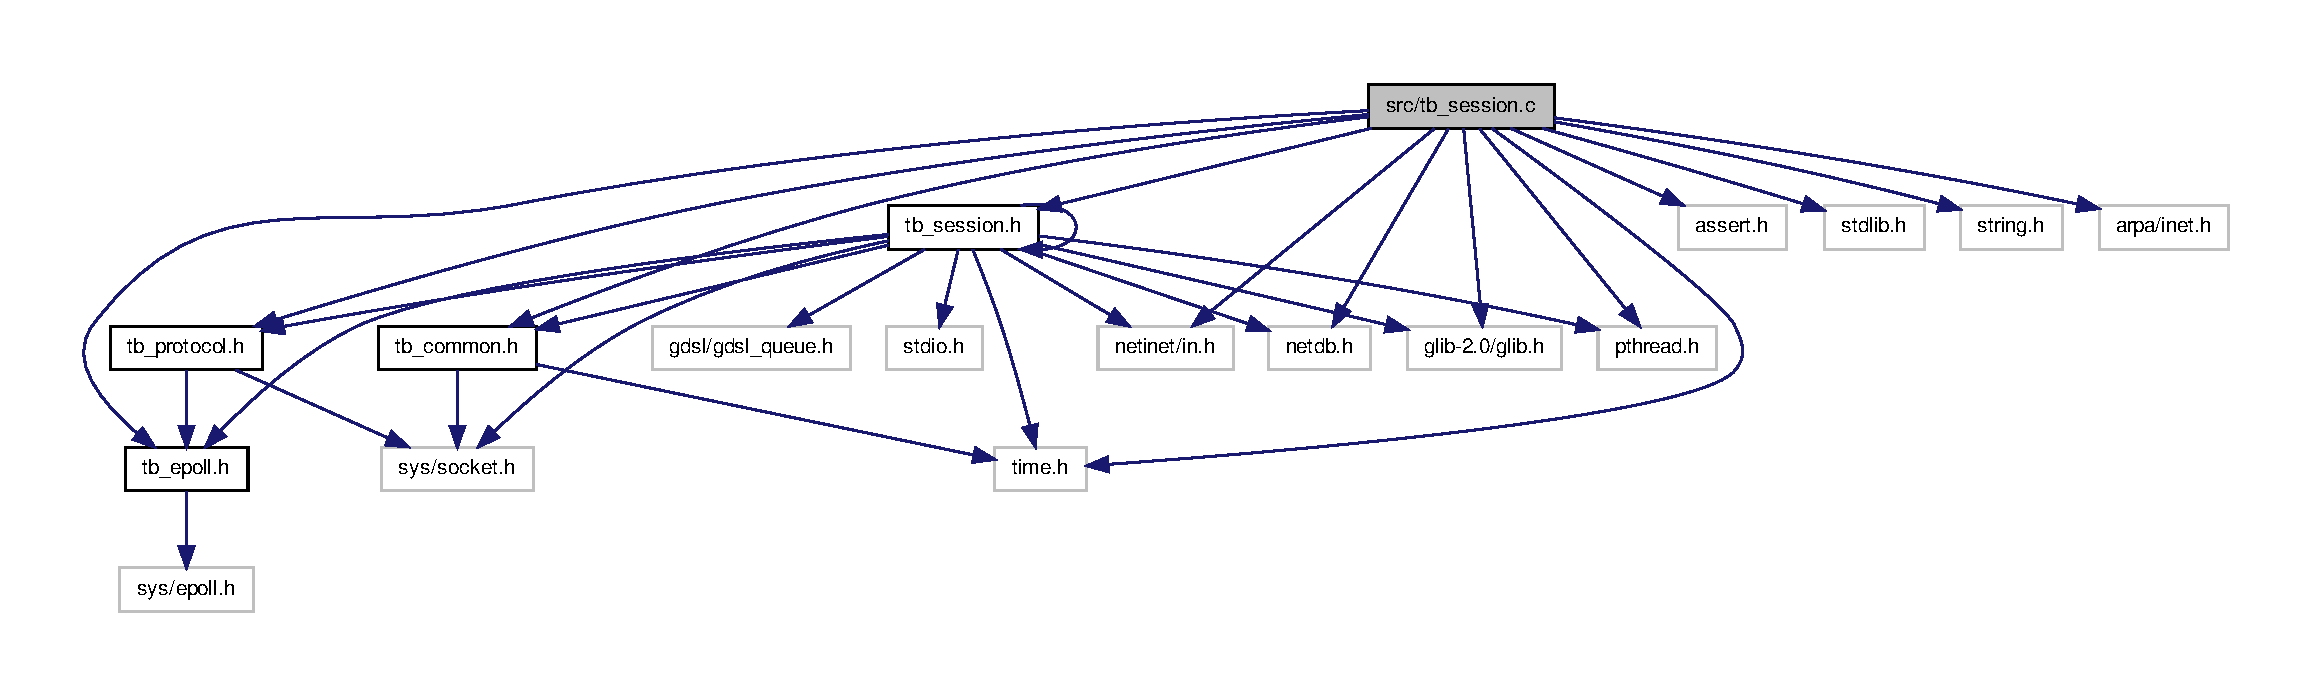
\includegraphics[width=350pt]{tb__session_8c__incl}
\end{center}
\end{figure}
\subsection*{Functions}
\begin{DoxyCompactItemize}
\item 
void \hyperlink{tb__session_8c_a15863848d0188bcb5662d43156903241}{tb\-\_\-session\-\_\-add} (\hyperlink{structtb__session__list__t}{tb\-\_\-session\-\_\-list\-\_\-t} $\ast$list, \hyperlink{structtb__session__t}{tb\-\_\-session\-\_\-t} $\ast$session)
\begin{DoxyCompactList}\small\item\em Add a session to a list. \end{DoxyCompactList}\item 
\hyperlink{structtb__session__t}{tb\-\_\-session\-\_\-t} $\ast$ \hyperlink{tb__session_8c_a2fc903815b77552836525068c01bda8b}{tb\-\_\-create\-\_\-server\-\_\-session} ()
\begin{DoxyCompactList}\small\item\em Create a session for servers. \end{DoxyCompactList}\item 
\hyperlink{structtb__session__t}{tb\-\_\-session\-\_\-t} $\ast$ \hyperlink{tb__session_8c_a3ae8d1d1ca5878cd9bab48098af09aae}{tb\-\_\-create\-\_\-session} ()
\begin{DoxyCompactList}\small\item\em Create a session. \end{DoxyCompactList}\item 
\hyperlink{structtb__session__t}{tb\-\_\-session\-\_\-t} $\ast$ \hyperlink{tb__session_8c_a61071ac6ac1fac65754a394e190fc57d}{tb\-\_\-create\-\_\-session\-\_\-full} (char $\ast$addr, char $\ast$port, int sock\-\_\-type, unsigned int data\-\_\-size)
\begin{DoxyCompactList}\small\item\em Full version of create session. \end{DoxyCompactList}\item 
void \hyperlink{tb__session_8c_a478a71afc34cc2f15ffd5732b102d5ca}{tb\-\_\-destroy\-\_\-session} (\hyperlink{structtb__session__t}{tb\-\_\-session\-\_\-t} $\ast$session)
\begin{DoxyCompactList}\small\item\em Free memory used for a session. \end{DoxyCompactList}\item 
int \hyperlink{tb__session_8c_ac07e93563e7b1e38af38e582e360ee02}{tb\-\_\-set\-\_\-addrinfo} (\hyperlink{structtb__session__t}{tb\-\_\-session\-\_\-t} $\ast$session, int type)
\begin{DoxyCompactList}\small\item\em Set the addrinfo for the session. \end{DoxyCompactList}\item 
void \hyperlink{tb__session_8c_a388990e2adbda494ee660b923afbf2db}{tb\-\_\-print\-\_\-times} (\hyperlink{structtb__session__t}{tb\-\_\-session\-\_\-t} $\ast$session)
\begin{DoxyCompactList}\small\item\em Print the times for a given session. \end{DoxyCompactList}\item 
gdsl\-\_\-element\-\_\-t \hyperlink{tb__session_8c_a45d4154769abcedc5989d6feeb106a5e}{allocate\-\_\-session} (void $\ast$data)
\begin{DoxyCompactList}\small\item\em Allocates memory for a session. \end{DoxyCompactList}\item 
void \hyperlink{tb__session_8c_a59019b05e88200313224bf2c77ae9c7a}{free\-\_\-session} (gdsl\-\_\-element\-\_\-t data)
\begin{DoxyCompactList}\small\item\em Free memory for a session. \end{DoxyCompactList}\item 
char $\ast$ \hyperlink{tb__session_8c_a61635f66121430da09247644cb1ba0f2}{get\-\_\-key\-\_\-value} (void $\ast$data)
\item 
gboolean \hyperlink{tb__session_8c_ac73265e0d989f9a9b1c1eeae3d290a09}{tb\-\_\-session\-\_\-equals} (gconstpointer a, gconstpointer b)
\begin{DoxyCompactList}\small\item\em Tests equality for sessions keys. \end{DoxyCompactList}\end{DoxyCompactItemize}


\subsection{Function Documentation}
\hypertarget{tb__session_8c_a45d4154769abcedc5989d6feeb106a5e}{\index{tb\-\_\-session.\-c@{tb\-\_\-session.\-c}!allocate\-\_\-session@{allocate\-\_\-session}}
\index{allocate\-\_\-session@{allocate\-\_\-session}!tb_session.c@{tb\-\_\-session.\-c}}
\subsubsection[{allocate\-\_\-session}]{\setlength{\rightskip}{0pt plus 5cm}gdsl\-\_\-element\-\_\-t allocate\-\_\-session (
\begin{DoxyParamCaption}
\item[{void $\ast$}]{data}
\end{DoxyParamCaption}
)}}\label{tb__session_8c_a45d4154769abcedc5989d6feeb106a5e}


Allocates memory for a session. 

Used by gdsl structures to allocate memory for a \hyperlink{structtb__session__t}{tb\-\_\-session\-\_\-t} struct.

data This needs to be an instance of \hyperlink{structtb__session__t}{tb\-\_\-session\-\_\-t} 

Definition at line 235 of file tb\-\_\-session.\-c.

\hypertarget{tb__session_8c_a59019b05e88200313224bf2c77ae9c7a}{\index{tb\-\_\-session.\-c@{tb\-\_\-session.\-c}!free\-\_\-session@{free\-\_\-session}}
\index{free\-\_\-session@{free\-\_\-session}!tb_session.c@{tb\-\_\-session.\-c}}
\subsubsection[{free\-\_\-session}]{\setlength{\rightskip}{0pt plus 5cm}void free\-\_\-session (
\begin{DoxyParamCaption}
\item[{gdsl\-\_\-element\-\_\-t}]{data}
\end{DoxyParamCaption}
)}}\label{tb__session_8c_a59019b05e88200313224bf2c77ae9c7a}


Free memory for a session. 



Definition at line 248 of file tb\-\_\-session.\-c.

\hypertarget{tb__session_8c_a61635f66121430da09247644cb1ba0f2}{\index{tb\-\_\-session.\-c@{tb\-\_\-session.\-c}!get\-\_\-key\-\_\-value@{get\-\_\-key\-\_\-value}}
\index{get\-\_\-key\-\_\-value@{get\-\_\-key\-\_\-value}!tb_session.c@{tb\-\_\-session.\-c}}
\subsubsection[{get\-\_\-key\-\_\-value}]{\setlength{\rightskip}{0pt plus 5cm}char$\ast$ get\-\_\-key\-\_\-value (
\begin{DoxyParamCaption}
\item[{void $\ast$}]{data}
\end{DoxyParamCaption}
)}}\label{tb__session_8c_a61635f66121430da09247644cb1ba0f2}


Definition at line 258 of file tb\-\_\-session.\-c.

\hypertarget{tb__session_8c_a2fc903815b77552836525068c01bda8b}{\index{tb\-\_\-session.\-c@{tb\-\_\-session.\-c}!tb\-\_\-create\-\_\-server\-\_\-session@{tb\-\_\-create\-\_\-server\-\_\-session}}
\index{tb\-\_\-create\-\_\-server\-\_\-session@{tb\-\_\-create\-\_\-server\-\_\-session}!tb_session.c@{tb\-\_\-session.\-c}}
\subsubsection[{tb\-\_\-create\-\_\-server\-\_\-session}]{\setlength{\rightskip}{0pt plus 5cm}{\bf tb\-\_\-session\-\_\-t}$\ast$ tb\-\_\-create\-\_\-server\-\_\-session (
\begin{DoxyParamCaption}
{}
\end{DoxyParamCaption}
)}}\label{tb__session_8c_a2fc903815b77552836525068c01bda8b}


Create a session for servers. 



Definition at line 44 of file tb\-\_\-session.\-c.

\hypertarget{tb__session_8c_a3ae8d1d1ca5878cd9bab48098af09aae}{\index{tb\-\_\-session.\-c@{tb\-\_\-session.\-c}!tb\-\_\-create\-\_\-session@{tb\-\_\-create\-\_\-session}}
\index{tb\-\_\-create\-\_\-session@{tb\-\_\-create\-\_\-session}!tb_session.c@{tb\-\_\-session.\-c}}
\subsubsection[{tb\-\_\-create\-\_\-session}]{\setlength{\rightskip}{0pt plus 5cm}{\bf tb\-\_\-session\-\_\-t}$\ast$ tb\-\_\-create\-\_\-session (
\begin{DoxyParamCaption}
{}
\end{DoxyParamCaption}
)}}\label{tb__session_8c_a3ae8d1d1ca5878cd9bab48098af09aae}


Create a session. 

With this version of create\-\_\-session, the sockaddr\-\_\-storage is created, the file name is set to N\-U\-L\-L, addr\-\_\-info and hints are null. 

Definition at line 59 of file tb\-\_\-session.\-c.

\hypertarget{tb__session_8c_a61071ac6ac1fac65754a394e190fc57d}{\index{tb\-\_\-session.\-c@{tb\-\_\-session.\-c}!tb\-\_\-create\-\_\-session\-\_\-full@{tb\-\_\-create\-\_\-session\-\_\-full}}
\index{tb\-\_\-create\-\_\-session\-\_\-full@{tb\-\_\-create\-\_\-session\-\_\-full}!tb_session.c@{tb\-\_\-session.\-c}}
\subsubsection[{tb\-\_\-create\-\_\-session\-\_\-full}]{\setlength{\rightskip}{0pt plus 5cm}{\bf tb\-\_\-session\-\_\-t}$\ast$ tb\-\_\-create\-\_\-session\-\_\-full (
\begin{DoxyParamCaption}
\item[{char $\ast$}]{addr, }
\item[{char $\ast$}]{port, }
\item[{int}]{sock\-\_\-type, }
\item[{unsigned int}]{data\-\_\-size}
\end{DoxyParamCaption}
)}}\label{tb__session_8c_a61071ac6ac1fac65754a394e190fc57d}


Full version of create session. 

This version creates the hints and info field, and resolves the provided address. If the data\-\_\-size parameter is greater than zero, the session buffer is also created. 

Definition at line 92 of file tb\-\_\-session.\-c.

\hypertarget{tb__session_8c_a478a71afc34cc2f15ffd5732b102d5ca}{\index{tb\-\_\-session.\-c@{tb\-\_\-session.\-c}!tb\-\_\-destroy\-\_\-session@{tb\-\_\-destroy\-\_\-session}}
\index{tb\-\_\-destroy\-\_\-session@{tb\-\_\-destroy\-\_\-session}!tb_session.c@{tb\-\_\-session.\-c}}
\subsubsection[{tb\-\_\-destroy\-\_\-session}]{\setlength{\rightskip}{0pt plus 5cm}void tb\-\_\-destroy\-\_\-session (
\begin{DoxyParamCaption}
\item[{{\bf tb\-\_\-session\-\_\-t} $\ast$}]{session}
\end{DoxyParamCaption}
)}}\label{tb__session_8c_a478a71afc34cc2f15ffd5732b102d5ca}


Free memory used for a session. 

Frees memory used by a \hyperlink{structtb__session__t}{tb\-\_\-session\-\_\-t} struct. Releases all memory for associated fields. 

Definition at line 117 of file tb\-\_\-session.\-c.

\hypertarget{tb__session_8c_a388990e2adbda494ee660b923afbf2db}{\index{tb\-\_\-session.\-c@{tb\-\_\-session.\-c}!tb\-\_\-print\-\_\-times@{tb\-\_\-print\-\_\-times}}
\index{tb\-\_\-print\-\_\-times@{tb\-\_\-print\-\_\-times}!tb_session.c@{tb\-\_\-session.\-c}}
\subsubsection[{tb\-\_\-print\-\_\-times}]{\setlength{\rightskip}{0pt plus 5cm}void tb\-\_\-print\-\_\-times (
\begin{DoxyParamCaption}
\item[{{\bf tb\-\_\-session\-\_\-t} $\ast$}]{session}
\end{DoxyParamCaption}
)}}\label{tb__session_8c_a388990e2adbda494ee660b923afbf2db}


Print the times for a given session. 

Prints to stdout the connection and transfer times for the given session.

\begin{DoxyPrecond}{Precondition}
The times in the session need to have been set, using the timer functions tb\-\_\-start\-\_\-time, tb\-\_\-finish\-\_\-time and tb\-\_\-calculate\-\_\-time 
\end{DoxyPrecond}

\begin{DoxyParams}{Parameters}
{\em session} & The session to print the times for. \\
\hline
\end{DoxyParams}


Definition at line 210 of file tb\-\_\-session.\-c.

\hypertarget{tb__session_8c_a15863848d0188bcb5662d43156903241}{\index{tb\-\_\-session.\-c@{tb\-\_\-session.\-c}!tb\-\_\-session\-\_\-add@{tb\-\_\-session\-\_\-add}}
\index{tb\-\_\-session\-\_\-add@{tb\-\_\-session\-\_\-add}!tb_session.c@{tb\-\_\-session.\-c}}
\subsubsection[{tb\-\_\-session\-\_\-add}]{\setlength{\rightskip}{0pt plus 5cm}void tb\-\_\-session\-\_\-add (
\begin{DoxyParamCaption}
\item[{{\bf tb\-\_\-session\-\_\-list\-\_\-t} $\ast$}]{list, }
\item[{{\bf tb\-\_\-session\-\_\-t} $\ast$}]{session}
\end{DoxyParamCaption}
)\hspace{0.3cm}{\ttfamily [inline]}}}\label{tb__session_8c_a15863848d0188bcb5662d43156903241}


Add a session to a list. 



Definition at line 25 of file tb\-\_\-session.\-c.

\hypertarget{tb__session_8c_ac73265e0d989f9a9b1c1eeae3d290a09}{\index{tb\-\_\-session.\-c@{tb\-\_\-session.\-c}!tb\-\_\-session\-\_\-equals@{tb\-\_\-session\-\_\-equals}}
\index{tb\-\_\-session\-\_\-equals@{tb\-\_\-session\-\_\-equals}!tb_session.c@{tb\-\_\-session.\-c}}
\subsubsection[{tb\-\_\-session\-\_\-equals}]{\setlength{\rightskip}{0pt plus 5cm}gboolean tb\-\_\-session\-\_\-equals (
\begin{DoxyParamCaption}
\item[{gconstpointer}]{a, }
\item[{gconstpointer}]{b}
\end{DoxyParamCaption}
)}}\label{tb__session_8c_ac73265e0d989f9a9b1c1eeae3d290a09}


Tests equality for sessions keys. 

Called by the hash table implementation in glib. Simply tests to see if the supplied integers are equal (these are just int32). 

Definition at line 281 of file tb\-\_\-session.\-c.

\hypertarget{tb__session_8c_ac07e93563e7b1e38af38e582e360ee02}{\index{tb\-\_\-session.\-c@{tb\-\_\-session.\-c}!tb\-\_\-set\-\_\-addrinfo@{tb\-\_\-set\-\_\-addrinfo}}
\index{tb\-\_\-set\-\_\-addrinfo@{tb\-\_\-set\-\_\-addrinfo}!tb_session.c@{tb\-\_\-session.\-c}}
\subsubsection[{tb\-\_\-set\-\_\-addrinfo}]{\setlength{\rightskip}{0pt plus 5cm}int tb\-\_\-set\-\_\-addrinfo (
\begin{DoxyParamCaption}
\item[{{\bf tb\-\_\-session\-\_\-t} $\ast$}]{session, }
\item[{int}]{type}
\end{DoxyParamCaption}
)}}\label{tb__session_8c_ac07e93563e7b1e38af38e582e360ee02}


Set the addrinfo for the session. 

Fills out the addrinfo field for the session. 

Definition at line 177 of file tb\-\_\-session.\-c.


\hypertarget{tb__session_8h}{\section{src/tb\-\_\-session.h File Reference}
\label{tb__session_8h}\index{src/tb\-\_\-session.\-h@{src/tb\-\_\-session.\-h}}
}
{\ttfamily \#include \char`\"{}tb\-\_\-epoll.\-h\char`\"{}}\\*
{\ttfamily \#include \char`\"{}tb\-\_\-common.\-h\char`\"{}}\\*
{\ttfamily \#include \char`\"{}tb\-\_\-session.\-h\char`\"{}}\\*
{\ttfamily \#include \char`\"{}tb\-\_\-protocol.\-h\char`\"{}}\\*
{\ttfamily \#include $<$gdsl/gdsl\-\_\-queue.\-h$>$}\\*
{\ttfamily \#include $<$netinet/in.\-h$>$}\\*
{\ttfamily \#include $<$sys/socket.\-h$>$}\\*
{\ttfamily \#include $<$stdio.\-h$>$}\\*
{\ttfamily \#include $<$time.\-h$>$}\\*
{\ttfamily \#include $<$netdb.\-h$>$}\\*
{\ttfamily \#include $<$glib-\/2.\-0/glib.\-h$>$}\\*
{\ttfamily \#include $<$pthread.\-h$>$}\\*
Include dependency graph for tb\-\_\-session.\-h\-:\nopagebreak
\begin{figure}[H]
\begin{center}
\leavevmode
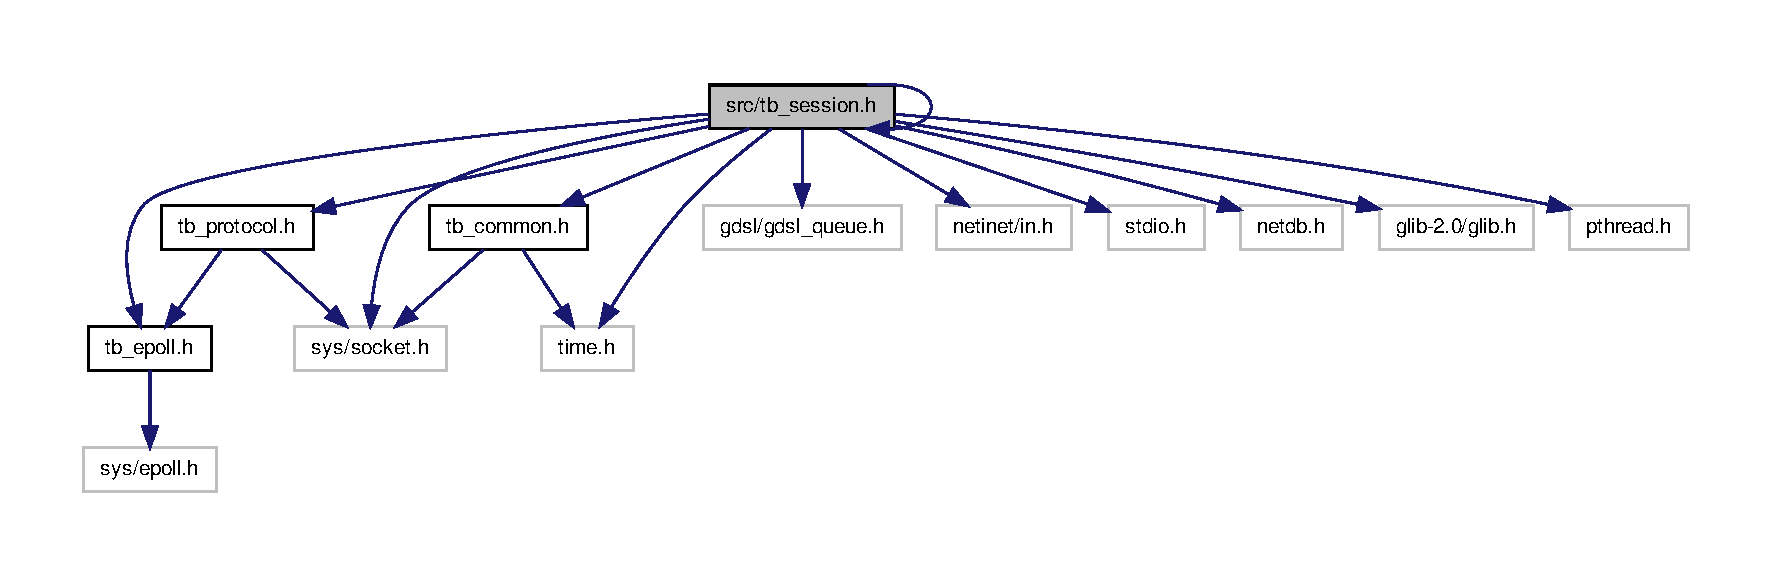
\includegraphics[width=350pt]{tb__session_8h__incl}
\end{center}
\end{figure}
This graph shows which files directly or indirectly include this file\-:\nopagebreak
\begin{figure}[H]
\begin{center}
\leavevmode
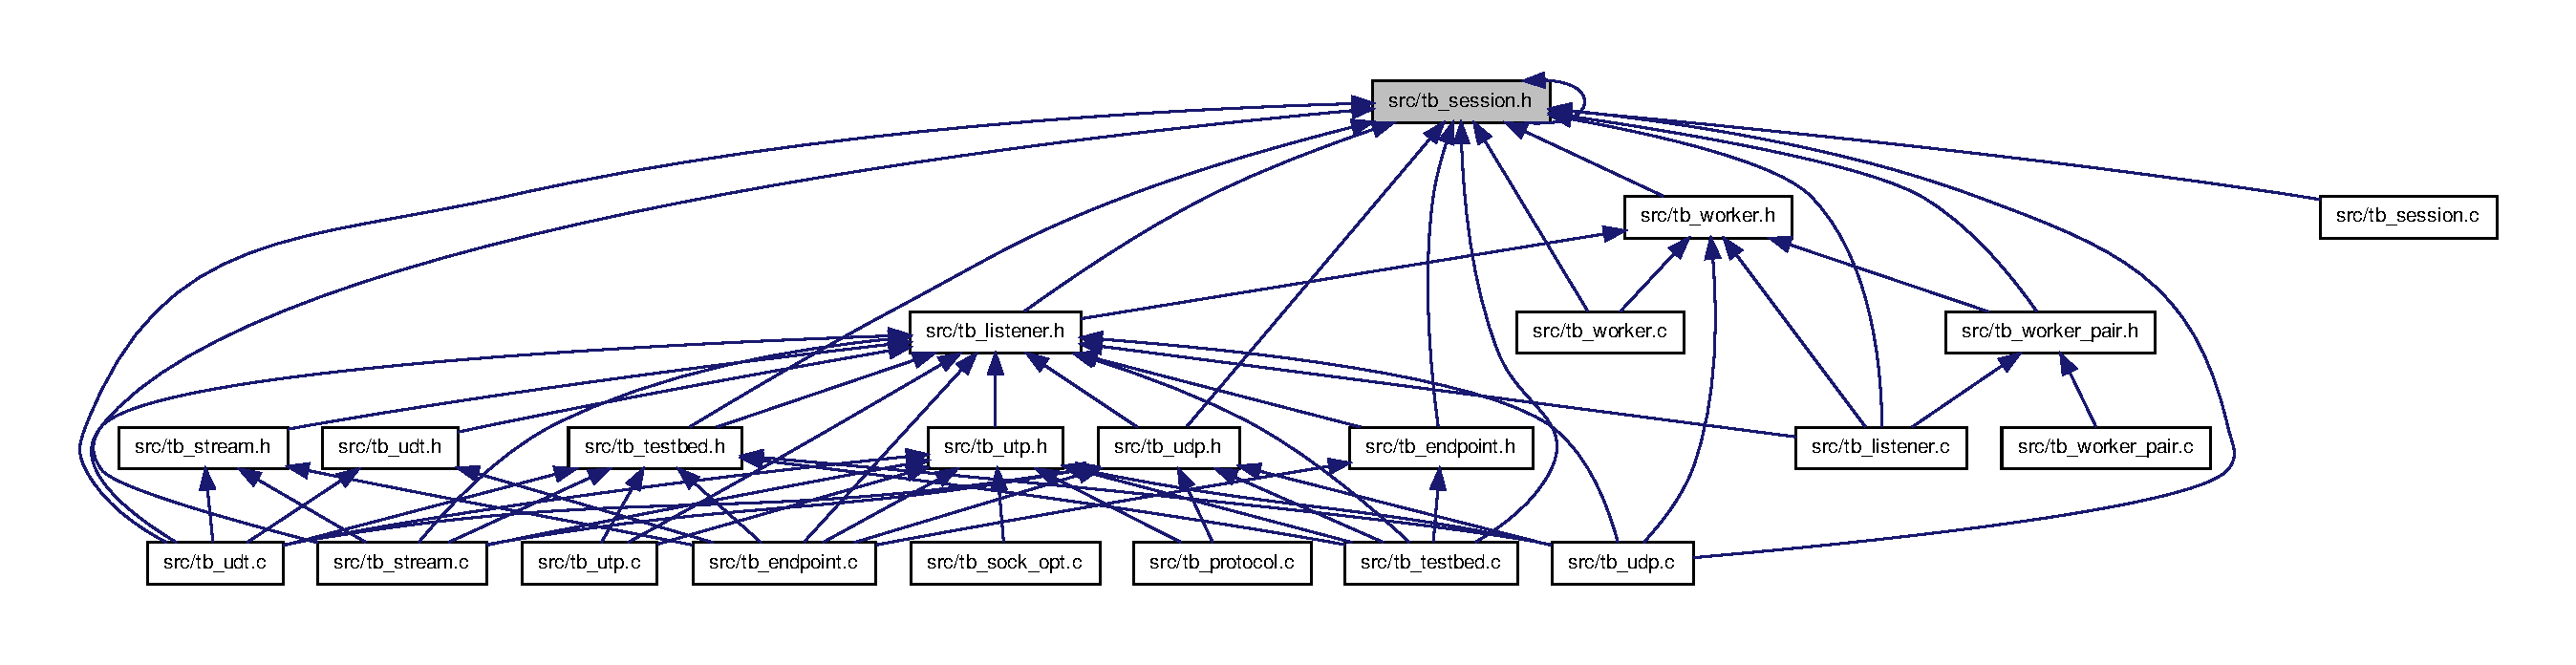
\includegraphics[width=350pt]{tb__session_8h__dep__incl}
\end{center}
\end{figure}
\subsection*{Data Structures}
\begin{DoxyCompactItemize}
\item 
struct \hyperlink{structtb__session__t}{tb\-\_\-session\-\_\-t}
\item 
struct \hyperlink{structtb__session__list__t}{tb\-\_\-session\-\_\-list\-\_\-t}
\end{DoxyCompactItemize}
\subsection*{Enumerations}
\begin{DoxyCompactItemize}
\item 
enum \hyperlink{tb__session_8h_a81168c33495c6f3db310119f82934596}{tb\-\_\-session\-\_\-status} \{ \\*
\hyperlink{tb__session_8h_a81168c33495c6f3db310119f82934596ac8e7bfb5416a21093e2568b1ae640266}{S\-E\-S\-S\-I\-O\-N\-\_\-\-C\-R\-E\-A\-T\-E\-D} =  0, 
\hyperlink{tb__session_8h_a81168c33495c6f3db310119f82934596a7c9bfcf1138bffa10f92669244ce322f}{S\-E\-S\-S\-I\-O\-N\-\_\-\-A\-D\-D\-R\-\_\-\-R\-E\-S}, 
\hyperlink{tb__session_8h_a81168c33495c6f3db310119f82934596aaeaf249bf530c55d32080954a6710513}{S\-E\-S\-S\-I\-O\-N\-\_\-\-C\-O\-N\-N\-E\-C\-T\-E\-D}, 
\hyperlink{tb__session_8h_a81168c33495c6f3db310119f82934596af8124514076dcacd530a96882aa18b43}{S\-E\-S\-S\-I\-O\-N\-\_\-\-C\-O\-M\-P\-L\-E\-T\-E}, 
\\*
\hyperlink{tb__session_8h_a81168c33495c6f3db310119f82934596a1dd86dbd444e24f2122e681e04a786d6}{S\-E\-S\-S\-I\-O\-N\-\_\-\-D\-I\-S\-C\-O\-N\-N\-E\-C\-T\-E\-D}
 \}
\item 
enum \hyperlink{tb__session_8h_a2fba7f46c36af12409fbd8310c057365}{tb\-\_\-session\-\_\-command} \{ \hyperlink{tb__session_8h_a2fba7f46c36af12409fbd8310c057365a8b126408d37dd3cd144b7015964e7806}{S\-\_\-\-C\-O\-N\-T\-I\-N\-U\-E} =  1, 
\hyperlink{tb__session_8h_a2fba7f46c36af12409fbd8310c057365a101f8f21c0766d2963d3b25eabbc6176}{S\-\_\-\-E\-X\-I\-T} =  2, 
\hyperlink{tb__session_8h_a2fba7f46c36af12409fbd8310c057365a4b4445bc1331335721a08eeb51fd6c1a}{S\-\_\-\-A\-B\-O\-R\-T} =  4, 
\hyperlink{tb__session_8h_a2fba7f46c36af12409fbd8310c057365acc296e4a2e71a0da7aa1b53db4473d72}{S\-\_\-\-E\-\_\-\-L\-O\-O\-P} =  S\-\_\-\-E\-X\-I\-T $|$ S\-\_\-\-A\-B\-O\-R\-T
 \}
\end{DoxyCompactItemize}
\subsection*{Functions}
\begin{DoxyCompactItemize}
\item 
void \hyperlink{tb__session_8h_ac78457e7ed21ef9c5a002d3752752d28}{tb\-\_\-session\-\_\-add} (\hyperlink{structtb__session__list__t}{tb\-\_\-session\-\_\-list\-\_\-t} $\ast$list, \hyperlink{structtb__session__t}{tb\-\_\-session\-\_\-t} $\ast$session) \-\_\-\-\_\-attribute\-\_\-\-\_\-((always\-\_\-inline))
\begin{DoxyCompactList}\small\item\em Add a session to a list. \end{DoxyCompactList}\item 
\hyperlink{structtb__session__t}{tb\-\_\-session\-\_\-t} $\ast$ \hyperlink{tb__session_8h_a2fc903815b77552836525068c01bda8b}{tb\-\_\-create\-\_\-server\-\_\-session} ()
\begin{DoxyCompactList}\small\item\em Create a session for servers. \end{DoxyCompactList}\item 
\hyperlink{structtb__session__t}{tb\-\_\-session\-\_\-t} $\ast$ \hyperlink{tb__session_8h_a3ae8d1d1ca5878cd9bab48098af09aae}{tb\-\_\-create\-\_\-session} ()
\begin{DoxyCompactList}\small\item\em Create a session. \end{DoxyCompactList}\item 
\hyperlink{structtb__session__t}{tb\-\_\-session\-\_\-t} $\ast$ \hyperlink{tb__session_8h_a61071ac6ac1fac65754a394e190fc57d}{tb\-\_\-create\-\_\-session\-\_\-full} (char $\ast$addr, char $\ast$port, int sock\-\_\-type, unsigned int data\-\_\-size)
\begin{DoxyCompactList}\small\item\em Full version of create session. \end{DoxyCompactList}\item 
void \hyperlink{tb__session_8h_a478a71afc34cc2f15ffd5732b102d5ca}{tb\-\_\-destroy\-\_\-session} (\hyperlink{structtb__session__t}{tb\-\_\-session\-\_\-t} $\ast$session)
\begin{DoxyCompactList}\small\item\em Free memory used for a session. \end{DoxyCompactList}\item 
int \hyperlink{tb__session_8h_ac07e93563e7b1e38af38e582e360ee02}{tb\-\_\-set\-\_\-addrinfo} (\hyperlink{structtb__session__t}{tb\-\_\-session\-\_\-t} $\ast$session, int type)
\begin{DoxyCompactList}\small\item\em Set the addrinfo for the session. \end{DoxyCompactList}\item 
void \hyperlink{tb__session_8h_a388990e2adbda494ee660b923afbf2db}{tb\-\_\-print\-\_\-times} (\hyperlink{structtb__session__t}{tb\-\_\-session\-\_\-t} $\ast$session)
\begin{DoxyCompactList}\small\item\em Print the times for a given session. \end{DoxyCompactList}\item 
gdsl\-\_\-element\-\_\-t \hyperlink{tb__session_8h_a45d4154769abcedc5989d6feeb106a5e}{allocate\-\_\-session} (void $\ast$data)
\begin{DoxyCompactList}\small\item\em Allocates memory for a session. \end{DoxyCompactList}\item 
void \hyperlink{tb__session_8h_a59019b05e88200313224bf2c77ae9c7a}{free\-\_\-session} (gdsl\-\_\-element\-\_\-t data)
\begin{DoxyCompactList}\small\item\em Free memory for a session. \end{DoxyCompactList}\item 
char $\ast$ \hyperlink{tb__session_8h_a61635f66121430da09247644cb1ba0f2}{get\-\_\-key\-\_\-value} (void $\ast$data)
\item 
gboolean \hyperlink{tb__session_8h_ac73265e0d989f9a9b1c1eeae3d290a09}{tb\-\_\-session\-\_\-equals} (gconstpointer a, gconstpointer b)
\begin{DoxyCompactList}\small\item\em Tests equality for sessions keys. \end{DoxyCompactList}\end{DoxyCompactItemize}


\subsection{Enumeration Type Documentation}
\hypertarget{tb__session_8h_a2fba7f46c36af12409fbd8310c057365}{\index{tb\-\_\-session.\-h@{tb\-\_\-session.\-h}!tb\-\_\-session\-\_\-command@{tb\-\_\-session\-\_\-command}}
\index{tb\-\_\-session\-\_\-command@{tb\-\_\-session\-\_\-command}!tb_session.h@{tb\-\_\-session.\-h}}
\subsubsection[{tb\-\_\-session\-\_\-command}]{\setlength{\rightskip}{0pt plus 5cm}enum {\bf tb\-\_\-session\-\_\-command}}}\label{tb__session_8h_a2fba7f46c36af12409fbd8310c057365}
\begin{Desc}
\item[Enumerator\-: ]\par
\begin{description}
\index{S\-\_\-\-C\-O\-N\-T\-I\-N\-U\-E@{S\-\_\-\-C\-O\-N\-T\-I\-N\-U\-E}!tb\-\_\-session.\-h@{tb\-\_\-session.\-h}}\index{tb\-\_\-session.\-h@{tb\-\_\-session.\-h}!S\-\_\-\-C\-O\-N\-T\-I\-N\-U\-E@{S\-\_\-\-C\-O\-N\-T\-I\-N\-U\-E}}\item[{\em 
\hypertarget{tb__session_8h_a2fba7f46c36af12409fbd8310c057365a8b126408d37dd3cd144b7015964e7806}{S\-\_\-\-C\-O\-N\-T\-I\-N\-U\-E}\label{tb__session_8h_a2fba7f46c36af12409fbd8310c057365a8b126408d37dd3cd144b7015964e7806}
}]\index{S\-\_\-\-E\-X\-I\-T@{S\-\_\-\-E\-X\-I\-T}!tb\-\_\-session.\-h@{tb\-\_\-session.\-h}}\index{tb\-\_\-session.\-h@{tb\-\_\-session.\-h}!S\-\_\-\-E\-X\-I\-T@{S\-\_\-\-E\-X\-I\-T}}\item[{\em 
\hypertarget{tb__session_8h_a2fba7f46c36af12409fbd8310c057365a101f8f21c0766d2963d3b25eabbc6176}{S\-\_\-\-E\-X\-I\-T}\label{tb__session_8h_a2fba7f46c36af12409fbd8310c057365a101f8f21c0766d2963d3b25eabbc6176}
}]\index{S\-\_\-\-A\-B\-O\-R\-T@{S\-\_\-\-A\-B\-O\-R\-T}!tb\-\_\-session.\-h@{tb\-\_\-session.\-h}}\index{tb\-\_\-session.\-h@{tb\-\_\-session.\-h}!S\-\_\-\-A\-B\-O\-R\-T@{S\-\_\-\-A\-B\-O\-R\-T}}\item[{\em 
\hypertarget{tb__session_8h_a2fba7f46c36af12409fbd8310c057365a4b4445bc1331335721a08eeb51fd6c1a}{S\-\_\-\-A\-B\-O\-R\-T}\label{tb__session_8h_a2fba7f46c36af12409fbd8310c057365a4b4445bc1331335721a08eeb51fd6c1a}
}]\index{S\-\_\-\-E\-\_\-\-L\-O\-O\-P@{S\-\_\-\-E\-\_\-\-L\-O\-O\-P}!tb\-\_\-session.\-h@{tb\-\_\-session.\-h}}\index{tb\-\_\-session.\-h@{tb\-\_\-session.\-h}!S\-\_\-\-E\-\_\-\-L\-O\-O\-P@{S\-\_\-\-E\-\_\-\-L\-O\-O\-P}}\item[{\em 
\hypertarget{tb__session_8h_a2fba7f46c36af12409fbd8310c057365acc296e4a2e71a0da7aa1b53db4473d72}{S\-\_\-\-E\-\_\-\-L\-O\-O\-P}\label{tb__session_8h_a2fba7f46c36af12409fbd8310c057365acc296e4a2e71a0da7aa1b53db4473d72}
}]\end{description}
\end{Desc}



Definition at line 35 of file tb\-\_\-session.\-h.

\hypertarget{tb__session_8h_a81168c33495c6f3db310119f82934596}{\index{tb\-\_\-session.\-h@{tb\-\_\-session.\-h}!tb\-\_\-session\-\_\-status@{tb\-\_\-session\-\_\-status}}
\index{tb\-\_\-session\-\_\-status@{tb\-\_\-session\-\_\-status}!tb_session.h@{tb\-\_\-session.\-h}}
\subsubsection[{tb\-\_\-session\-\_\-status}]{\setlength{\rightskip}{0pt plus 5cm}enum {\bf tb\-\_\-session\-\_\-status}}}\label{tb__session_8h_a81168c33495c6f3db310119f82934596}
\begin{Desc}
\item[Enumerator\-: ]\par
\begin{description}
\index{S\-E\-S\-S\-I\-O\-N\-\_\-\-C\-R\-E\-A\-T\-E\-D@{S\-E\-S\-S\-I\-O\-N\-\_\-\-C\-R\-E\-A\-T\-E\-D}!tb\-\_\-session.\-h@{tb\-\_\-session.\-h}}\index{tb\-\_\-session.\-h@{tb\-\_\-session.\-h}!S\-E\-S\-S\-I\-O\-N\-\_\-\-C\-R\-E\-A\-T\-E\-D@{S\-E\-S\-S\-I\-O\-N\-\_\-\-C\-R\-E\-A\-T\-E\-D}}\item[{\em 
\hypertarget{tb__session_8h_a81168c33495c6f3db310119f82934596ac8e7bfb5416a21093e2568b1ae640266}{S\-E\-S\-S\-I\-O\-N\-\_\-\-C\-R\-E\-A\-T\-E\-D}\label{tb__session_8h_a81168c33495c6f3db310119f82934596ac8e7bfb5416a21093e2568b1ae640266}
}]\index{S\-E\-S\-S\-I\-O\-N\-\_\-\-A\-D\-D\-R\-\_\-\-R\-E\-S@{S\-E\-S\-S\-I\-O\-N\-\_\-\-A\-D\-D\-R\-\_\-\-R\-E\-S}!tb\-\_\-session.\-h@{tb\-\_\-session.\-h}}\index{tb\-\_\-session.\-h@{tb\-\_\-session.\-h}!S\-E\-S\-S\-I\-O\-N\-\_\-\-A\-D\-D\-R\-\_\-\-R\-E\-S@{S\-E\-S\-S\-I\-O\-N\-\_\-\-A\-D\-D\-R\-\_\-\-R\-E\-S}}\item[{\em 
\hypertarget{tb__session_8h_a81168c33495c6f3db310119f82934596a7c9bfcf1138bffa10f92669244ce322f}{S\-E\-S\-S\-I\-O\-N\-\_\-\-A\-D\-D\-R\-\_\-\-R\-E\-S}\label{tb__session_8h_a81168c33495c6f3db310119f82934596a7c9bfcf1138bffa10f92669244ce322f}
}]\index{S\-E\-S\-S\-I\-O\-N\-\_\-\-C\-O\-N\-N\-E\-C\-T\-E\-D@{S\-E\-S\-S\-I\-O\-N\-\_\-\-C\-O\-N\-N\-E\-C\-T\-E\-D}!tb\-\_\-session.\-h@{tb\-\_\-session.\-h}}\index{tb\-\_\-session.\-h@{tb\-\_\-session.\-h}!S\-E\-S\-S\-I\-O\-N\-\_\-\-C\-O\-N\-N\-E\-C\-T\-E\-D@{S\-E\-S\-S\-I\-O\-N\-\_\-\-C\-O\-N\-N\-E\-C\-T\-E\-D}}\item[{\em 
\hypertarget{tb__session_8h_a81168c33495c6f3db310119f82934596aaeaf249bf530c55d32080954a6710513}{S\-E\-S\-S\-I\-O\-N\-\_\-\-C\-O\-N\-N\-E\-C\-T\-E\-D}\label{tb__session_8h_a81168c33495c6f3db310119f82934596aaeaf249bf530c55d32080954a6710513}
}]\index{S\-E\-S\-S\-I\-O\-N\-\_\-\-C\-O\-M\-P\-L\-E\-T\-E@{S\-E\-S\-S\-I\-O\-N\-\_\-\-C\-O\-M\-P\-L\-E\-T\-E}!tb\-\_\-session.\-h@{tb\-\_\-session.\-h}}\index{tb\-\_\-session.\-h@{tb\-\_\-session.\-h}!S\-E\-S\-S\-I\-O\-N\-\_\-\-C\-O\-M\-P\-L\-E\-T\-E@{S\-E\-S\-S\-I\-O\-N\-\_\-\-C\-O\-M\-P\-L\-E\-T\-E}}\item[{\em 
\hypertarget{tb__session_8h_a81168c33495c6f3db310119f82934596af8124514076dcacd530a96882aa18b43}{S\-E\-S\-S\-I\-O\-N\-\_\-\-C\-O\-M\-P\-L\-E\-T\-E}\label{tb__session_8h_a81168c33495c6f3db310119f82934596af8124514076dcacd530a96882aa18b43}
}]\index{S\-E\-S\-S\-I\-O\-N\-\_\-\-D\-I\-S\-C\-O\-N\-N\-E\-C\-T\-E\-D@{S\-E\-S\-S\-I\-O\-N\-\_\-\-D\-I\-S\-C\-O\-N\-N\-E\-C\-T\-E\-D}!tb\-\_\-session.\-h@{tb\-\_\-session.\-h}}\index{tb\-\_\-session.\-h@{tb\-\_\-session.\-h}!S\-E\-S\-S\-I\-O\-N\-\_\-\-D\-I\-S\-C\-O\-N\-N\-E\-C\-T\-E\-D@{S\-E\-S\-S\-I\-O\-N\-\_\-\-D\-I\-S\-C\-O\-N\-N\-E\-C\-T\-E\-D}}\item[{\em 
\hypertarget{tb__session_8h_a81168c33495c6f3db310119f82934596a1dd86dbd444e24f2122e681e04a786d6}{S\-E\-S\-S\-I\-O\-N\-\_\-\-D\-I\-S\-C\-O\-N\-N\-E\-C\-T\-E\-D}\label{tb__session_8h_a81168c33495c6f3db310119f82934596a1dd86dbd444e24f2122e681e04a786d6}
}]\end{description}
\end{Desc}



Definition at line 25 of file tb\-\_\-session.\-h.



\subsection{Function Documentation}
\hypertarget{tb__session_8h_a45d4154769abcedc5989d6feeb106a5e}{\index{tb\-\_\-session.\-h@{tb\-\_\-session.\-h}!allocate\-\_\-session@{allocate\-\_\-session}}
\index{allocate\-\_\-session@{allocate\-\_\-session}!tb_session.h@{tb\-\_\-session.\-h}}
\subsubsection[{allocate\-\_\-session}]{\setlength{\rightskip}{0pt plus 5cm}gdsl\-\_\-element\-\_\-t allocate\-\_\-session (
\begin{DoxyParamCaption}
\item[{void $\ast$}]{data}
\end{DoxyParamCaption}
)}}\label{tb__session_8h_a45d4154769abcedc5989d6feeb106a5e}


Allocates memory for a session. 

Used by gdsl structures to allocate memory for a \hyperlink{structtb__session__t}{tb\-\_\-session\-\_\-t} struct.

data This needs to be an instance of \hyperlink{structtb__session__t}{tb\-\_\-session\-\_\-t} 

Definition at line 235 of file tb\-\_\-session.\-c.

\hypertarget{tb__session_8h_a59019b05e88200313224bf2c77ae9c7a}{\index{tb\-\_\-session.\-h@{tb\-\_\-session.\-h}!free\-\_\-session@{free\-\_\-session}}
\index{free\-\_\-session@{free\-\_\-session}!tb_session.h@{tb\-\_\-session.\-h}}
\subsubsection[{free\-\_\-session}]{\setlength{\rightskip}{0pt plus 5cm}void free\-\_\-session (
\begin{DoxyParamCaption}
\item[{gdsl\-\_\-element\-\_\-t}]{data}
\end{DoxyParamCaption}
)}}\label{tb__session_8h_a59019b05e88200313224bf2c77ae9c7a}


Free memory for a session. 



Definition at line 248 of file tb\-\_\-session.\-c.

\hypertarget{tb__session_8h_a61635f66121430da09247644cb1ba0f2}{\index{tb\-\_\-session.\-h@{tb\-\_\-session.\-h}!get\-\_\-key\-\_\-value@{get\-\_\-key\-\_\-value}}
\index{get\-\_\-key\-\_\-value@{get\-\_\-key\-\_\-value}!tb_session.h@{tb\-\_\-session.\-h}}
\subsubsection[{get\-\_\-key\-\_\-value}]{\setlength{\rightskip}{0pt plus 5cm}char$\ast$ get\-\_\-key\-\_\-value (
\begin{DoxyParamCaption}
\item[{void $\ast$}]{data}
\end{DoxyParamCaption}
)}}\label{tb__session_8h_a61635f66121430da09247644cb1ba0f2}


Definition at line 258 of file tb\-\_\-session.\-c.

\hypertarget{tb__session_8h_a2fc903815b77552836525068c01bda8b}{\index{tb\-\_\-session.\-h@{tb\-\_\-session.\-h}!tb\-\_\-create\-\_\-server\-\_\-session@{tb\-\_\-create\-\_\-server\-\_\-session}}
\index{tb\-\_\-create\-\_\-server\-\_\-session@{tb\-\_\-create\-\_\-server\-\_\-session}!tb_session.h@{tb\-\_\-session.\-h}}
\subsubsection[{tb\-\_\-create\-\_\-server\-\_\-session}]{\setlength{\rightskip}{0pt plus 5cm}{\bf tb\-\_\-session\-\_\-t}$\ast$ tb\-\_\-create\-\_\-server\-\_\-session (
\begin{DoxyParamCaption}
{}
\end{DoxyParamCaption}
)}}\label{tb__session_8h_a2fc903815b77552836525068c01bda8b}


Create a session for servers. 



Definition at line 44 of file tb\-\_\-session.\-c.

\hypertarget{tb__session_8h_a3ae8d1d1ca5878cd9bab48098af09aae}{\index{tb\-\_\-session.\-h@{tb\-\_\-session.\-h}!tb\-\_\-create\-\_\-session@{tb\-\_\-create\-\_\-session}}
\index{tb\-\_\-create\-\_\-session@{tb\-\_\-create\-\_\-session}!tb_session.h@{tb\-\_\-session.\-h}}
\subsubsection[{tb\-\_\-create\-\_\-session}]{\setlength{\rightskip}{0pt plus 5cm}{\bf tb\-\_\-session\-\_\-t}$\ast$ tb\-\_\-create\-\_\-session (
\begin{DoxyParamCaption}
{}
\end{DoxyParamCaption}
)}}\label{tb__session_8h_a3ae8d1d1ca5878cd9bab48098af09aae}


Create a session. 

With this version of create\-\_\-session, the sockaddr\-\_\-storage is created, the file name is set to N\-U\-L\-L, addr\-\_\-info and hints are null. 

Definition at line 59 of file tb\-\_\-session.\-c.

\hypertarget{tb__session_8h_a61071ac6ac1fac65754a394e190fc57d}{\index{tb\-\_\-session.\-h@{tb\-\_\-session.\-h}!tb\-\_\-create\-\_\-session\-\_\-full@{tb\-\_\-create\-\_\-session\-\_\-full}}
\index{tb\-\_\-create\-\_\-session\-\_\-full@{tb\-\_\-create\-\_\-session\-\_\-full}!tb_session.h@{tb\-\_\-session.\-h}}
\subsubsection[{tb\-\_\-create\-\_\-session\-\_\-full}]{\setlength{\rightskip}{0pt plus 5cm}{\bf tb\-\_\-session\-\_\-t}$\ast$ tb\-\_\-create\-\_\-session\-\_\-full (
\begin{DoxyParamCaption}
\item[{char $\ast$}]{addr, }
\item[{char $\ast$}]{port, }
\item[{int}]{sock\-\_\-type, }
\item[{unsigned int}]{data\-\_\-size}
\end{DoxyParamCaption}
)}}\label{tb__session_8h_a61071ac6ac1fac65754a394e190fc57d}


Full version of create session. 

This version creates the hints and info field, and resolves the provided address. If the data\-\_\-size parameter is greater than zero, the session buffer is also created. 

Definition at line 92 of file tb\-\_\-session.\-c.

\hypertarget{tb__session_8h_a478a71afc34cc2f15ffd5732b102d5ca}{\index{tb\-\_\-session.\-h@{tb\-\_\-session.\-h}!tb\-\_\-destroy\-\_\-session@{tb\-\_\-destroy\-\_\-session}}
\index{tb\-\_\-destroy\-\_\-session@{tb\-\_\-destroy\-\_\-session}!tb_session.h@{tb\-\_\-session.\-h}}
\subsubsection[{tb\-\_\-destroy\-\_\-session}]{\setlength{\rightskip}{0pt plus 5cm}void tb\-\_\-destroy\-\_\-session (
\begin{DoxyParamCaption}
\item[{{\bf tb\-\_\-session\-\_\-t} $\ast$}]{session}
\end{DoxyParamCaption}
)}}\label{tb__session_8h_a478a71afc34cc2f15ffd5732b102d5ca}


Free memory used for a session. 

Frees memory used by a \hyperlink{structtb__session__t}{tb\-\_\-session\-\_\-t} struct. Releases all memory for associated fields. 

Definition at line 117 of file tb\-\_\-session.\-c.

\hypertarget{tb__session_8h_a388990e2adbda494ee660b923afbf2db}{\index{tb\-\_\-session.\-h@{tb\-\_\-session.\-h}!tb\-\_\-print\-\_\-times@{tb\-\_\-print\-\_\-times}}
\index{tb\-\_\-print\-\_\-times@{tb\-\_\-print\-\_\-times}!tb_session.h@{tb\-\_\-session.\-h}}
\subsubsection[{tb\-\_\-print\-\_\-times}]{\setlength{\rightskip}{0pt plus 5cm}void tb\-\_\-print\-\_\-times (
\begin{DoxyParamCaption}
\item[{{\bf tb\-\_\-session\-\_\-t} $\ast$}]{session}
\end{DoxyParamCaption}
)}}\label{tb__session_8h_a388990e2adbda494ee660b923afbf2db}


Print the times for a given session. 

Prints to stdout the connection and transfer times for the given session.

\begin{DoxyPrecond}{Precondition}
The times in the session need to have been set, using the timer functions tb\-\_\-start\-\_\-time, tb\-\_\-finish\-\_\-time and tb\-\_\-calculate\-\_\-time 
\end{DoxyPrecond}

\begin{DoxyParams}{Parameters}
{\em session} & The session to print the times for. \\
\hline
\end{DoxyParams}


Definition at line 210 of file tb\-\_\-session.\-c.

\hypertarget{tb__session_8h_ac78457e7ed21ef9c5a002d3752752d28}{\index{tb\-\_\-session.\-h@{tb\-\_\-session.\-h}!tb\-\_\-session\-\_\-add@{tb\-\_\-session\-\_\-add}}
\index{tb\-\_\-session\-\_\-add@{tb\-\_\-session\-\_\-add}!tb_session.h@{tb\-\_\-session.\-h}}
\subsubsection[{tb\-\_\-session\-\_\-add}]{\setlength{\rightskip}{0pt plus 5cm}void tb\-\_\-session\-\_\-add (
\begin{DoxyParamCaption}
\item[{{\bf tb\-\_\-session\-\_\-list\-\_\-t} $\ast$}]{list, }
\item[{{\bf tb\-\_\-session\-\_\-t} $\ast$}]{session}
\end{DoxyParamCaption}
)\hspace{0.3cm}{\ttfamily [inline]}}}\label{tb__session_8h_ac78457e7ed21ef9c5a002d3752752d28}


Add a session to a list. 



Definition at line 25 of file tb\-\_\-session.\-c.

\hypertarget{tb__session_8h_ac73265e0d989f9a9b1c1eeae3d290a09}{\index{tb\-\_\-session.\-h@{tb\-\_\-session.\-h}!tb\-\_\-session\-\_\-equals@{tb\-\_\-session\-\_\-equals}}
\index{tb\-\_\-session\-\_\-equals@{tb\-\_\-session\-\_\-equals}!tb_session.h@{tb\-\_\-session.\-h}}
\subsubsection[{tb\-\_\-session\-\_\-equals}]{\setlength{\rightskip}{0pt plus 5cm}gboolean tb\-\_\-session\-\_\-equals (
\begin{DoxyParamCaption}
\item[{gconstpointer}]{a, }
\item[{gconstpointer}]{b}
\end{DoxyParamCaption}
)}}\label{tb__session_8h_ac73265e0d989f9a9b1c1eeae3d290a09}


Tests equality for sessions keys. 

Called by the hash table implementation in glib. Simply tests to see if the supplied integers are equal (these are just int32). 

Definition at line 281 of file tb\-\_\-session.\-c.

\hypertarget{tb__session_8h_ac07e93563e7b1e38af38e582e360ee02}{\index{tb\-\_\-session.\-h@{tb\-\_\-session.\-h}!tb\-\_\-set\-\_\-addrinfo@{tb\-\_\-set\-\_\-addrinfo}}
\index{tb\-\_\-set\-\_\-addrinfo@{tb\-\_\-set\-\_\-addrinfo}!tb_session.h@{tb\-\_\-session.\-h}}
\subsubsection[{tb\-\_\-set\-\_\-addrinfo}]{\setlength{\rightskip}{0pt plus 5cm}int tb\-\_\-set\-\_\-addrinfo (
\begin{DoxyParamCaption}
\item[{{\bf tb\-\_\-session\-\_\-t} $\ast$}]{session, }
\item[{int}]{type}
\end{DoxyParamCaption}
)}}\label{tb__session_8h_ac07e93563e7b1e38af38e582e360ee02}


Set the addrinfo for the session. 

Fills out the addrinfo field for the session. 

Definition at line 177 of file tb\-\_\-session.\-c.


\hypertarget{tb__sock__opt_8c}{\section{src/tb\-\_\-sock\-\_\-opt.c File Reference}
\label{tb__sock__opt_8c}\index{src/tb\-\_\-sock\-\_\-opt.\-c@{src/tb\-\_\-sock\-\_\-opt.\-c}}
}
{\ttfamily \#include \char`\"{}tb\-\_\-sock\-\_\-opt.\-h\char`\"{}}\\*
{\ttfamily \#include \char`\"{}tb\-\_\-protocol.\-h\char`\"{}}\\*
{\ttfamily \#include \char`\"{}tb\-\_\-common.\-h\char`\"{}}\\*
{\ttfamily \#include \char`\"{}tb\-\_\-utp.\-h\char`\"{}}\\*
{\ttfamily \#include $<$sys/socket.\-h$>$}\\*
{\ttfamily \#include $<$netdb.\-h$>$}\\*
{\ttfamily \#include $<$arpa/inet.\-h$>$}\\*
{\ttfamily \#include $<$fcntl.\-h$>$}\\*
Include dependency graph for tb\-\_\-sock\-\_\-opt.\-c\-:\nopagebreak
\begin{figure}[H]
\begin{center}
\leavevmode
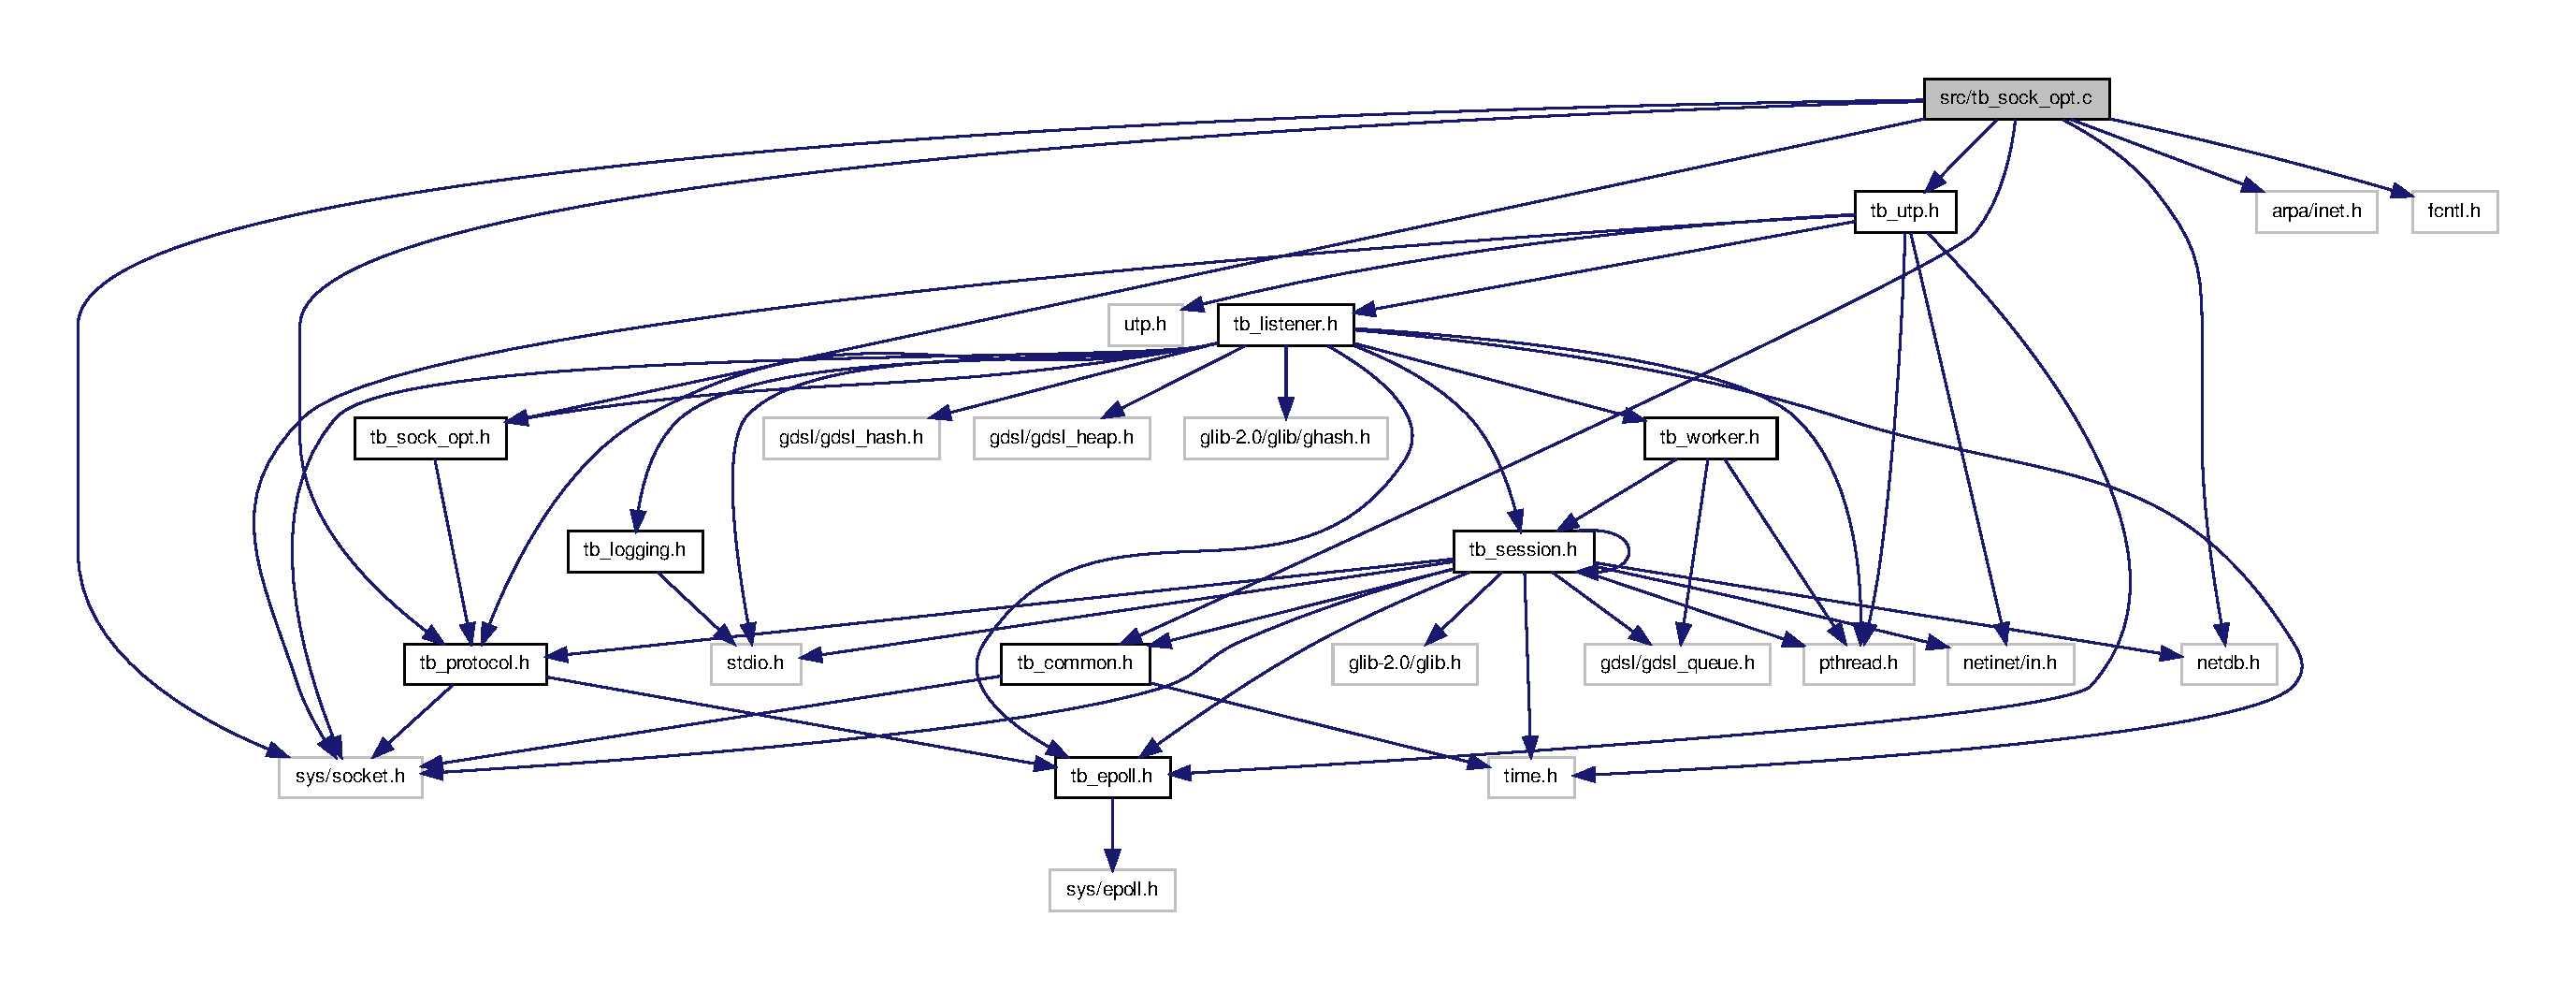
\includegraphics[width=350pt]{tb__sock__opt_8c__incl}
\end{center}
\end{figure}
\subsection*{Functions}
\begin{DoxyCompactItemize}
\item 
int \hyperlink{tb__sock__opt_8c_a43b2b5e868cfb51f3e8ad367d8f354e8}{tb\-\_\-set\-\_\-sock\-\_\-opt} (\hyperlink{structtb__options__t}{tb\-\_\-options\-\_\-t} $\ast$options, int fd)
\begin{DoxyCompactList}\small\item\em Set options for individual protocols. \end{DoxyCompactList}\item 
int \hyperlink{tb__sock__opt_8c_aeb90bdb9face6f1bbe2e7c141a428cdf}{tb\-\_\-set\-\_\-bsd\-\_\-sock\-\_\-opts} (\hyperlink{structtb__options__t}{tb\-\_\-options\-\_\-t} $\ast$options, int fd)
\begin{DoxyCompactList}\small\item\em Set options for B\-S\-D sockets. Used by T\-C\-P, U\-D\-P and e\-U\-D\-P. \end{DoxyCompactList}\item 
int \hyperlink{tb__sock__opt_8c_a0c80d1c0e50d1312798c17f7f1add6e2}{tb\-\_\-set\-\_\-tcp\-\_\-opts} (\hyperlink{structtb__options__t}{tb\-\_\-options\-\_\-t} $\ast$options, int fd)
\begin{DoxyCompactList}\small\item\em Set options for T\-C\-P. \end{DoxyCompactList}\item 
int \hyperlink{tb__sock__opt_8c_af776cbfef331b9154f4cb40888e75bae}{tb\-\_\-set\-\_\-udp\-\_\-opts} (\hyperlink{structtb__options__t}{tb\-\_\-options\-\_\-t} $\ast$options, int fd)
\begin{DoxyCompactList}\small\item\em Set options for U\-D\-P. \end{DoxyCompactList}\item 
int \hyperlink{tb__sock__opt_8c_a834ce1097c65130cf74f1695eff08b1c}{tb\-\_\-set\-\_\-udt\-\_\-opts} (\hyperlink{structtb__options__t}{tb\-\_\-options\-\_\-t} $\ast$options, int fd)
\begin{DoxyCompactList}\small\item\em Set options for U\-D\-T. \end{DoxyCompactList}\item 
int \hyperlink{tb__sock__opt_8c_a178a04119b0fa7767e32fe915832c33e}{tb\-\_\-set\-\_\-audt\-\_\-opts} (\hyperlink{structtb__options__t}{tb\-\_\-options\-\_\-t} $\ast$options, int fd)
\begin{DoxyCompactList}\small\item\em Set options for a\-U\-D\-T. \end{DoxyCompactList}\item 
int \hyperlink{tb__sock__opt_8c_ac991c8bf8191d0900eac41096eeb3ab9}{tb\-\_\-set\-\_\-utp\-\_\-opts} (\hyperlink{structtb__options__t}{tb\-\_\-options\-\_\-t} $\ast$options, int fd)
\begin{DoxyCompactList}\small\item\em Set options for u\-T\-P. \end{DoxyCompactList}\item 
int \hyperlink{tb__sock__opt_8c_a3e68a727c2d788a487f8a973aec788f2}{tb\-\_\-set\-\_\-eudp\-\_\-opts} (\hyperlink{structtb__options__t}{tb\-\_\-options\-\_\-t} $\ast$options, int fd)
\begin{DoxyCompactList}\small\item\em Set options for e\-U\-D\-P. \end{DoxyCompactList}\item 
int \hyperlink{tb__sock__opt_8c_a1740be02ba9a1f9372be0ac2b4061f99}{tb\-\_\-set\-\_\-dccp\-\_\-opts} (\hyperlink{structtb__options__t}{tb\-\_\-options\-\_\-t} $\ast$options, int fd)
\begin{DoxyCompactList}\small\item\em Set options for D\-C\-C\-P. \end{DoxyCompactList}\end{DoxyCompactItemize}
\subsection*{Variables}
\begin{DoxyCompactItemize}
\item 
const int \hyperlink{tb__sock__opt_8c_a546259a497fb4f4a2ed3eca4f2df8c7b}{U\-D\-T\-\_\-\-S\-N\-D\-\_\-\-B\-U\-F\-F} = 1024 $\ast$ 1024 $\ast$ 10
\item 
const int \hyperlink{tb__sock__opt_8c_a336fb201b76af68ff4518278ac94ab06}{U\-D\-T\-\_\-\-R\-C\-V\-\_\-\-B\-U\-F\-F} = 1024 $\ast$ 1024 $\ast$ 10
\item 
const int \hyperlink{tb__sock__opt_8c_a0b316e118833d3d23071779fce32ee32}{U\-D\-P\-\_\-\-S\-N\-D\-\_\-\-B\-U\-F\-F} = 1024 $\ast$ 256
\item 
const int \hyperlink{tb__sock__opt_8c_aa5a5320a53c72b290f4027b8b858024c}{U\-D\-P\-\_\-\-R\-C\-V\-\_\-\-B\-U\-F\-F} = 1024 $\ast$ 1024
\item 
const int \hyperlink{tb__sock__opt_8c_ab2ce54d61f26ea80ae2ce7990537a51a}{T\-C\-P\-\_\-\-S\-N\-D\-\_\-\-B\-U\-F\-F} = 1024 $\ast$ 256
\item 
const int \hyperlink{tb__sock__opt_8c_a6614561194a3b54264c01d7b7eba4b75}{T\-C\-P\-\_\-\-R\-C\-V\-\_\-\-B\-U\-F\-F} = 1024 $\ast$ 1024
\item 
const int \hyperlink{tb__sock__opt_8c_a6fc4fd2ac14035fda584b5a66634d395}{u\-T\-P\-\_\-\-S\-N\-D\-\_\-\-B\-U\-F\-F} = 300 $\ast$ 200
\item 
const int \hyperlink{tb__sock__opt_8c_afa8d1866976a282df203e70aaad012d0}{u\-T\-P\-\_\-\-R\-C\-V\-\_\-\-B\-U\-F\-F} = 300 $\ast$ 200
\item 
const int \hyperlink{tb__sock__opt_8c_aef7d89138e6b529c349b6cdb2ab021cd}{D\-C\-C\-P\-\_\-\-S\-N\-D\-\_\-\-B\-U\-F\-F} = 1024 $\ast$ 256
\item 
const int \hyperlink{tb__sock__opt_8c_a934abdd1dd88c196b5a0a64ab231aaa4}{D\-C\-C\-P\-\_\-\-R\-C\-V\-\_\-\-B\-U\-F\-F} = 1024 $\ast$ 1024
\end{DoxyCompactItemize}


\subsection{Function Documentation}
\hypertarget{tb__sock__opt_8c_a178a04119b0fa7767e32fe915832c33e}{\index{tb\-\_\-sock\-\_\-opt.\-c@{tb\-\_\-sock\-\_\-opt.\-c}!tb\-\_\-set\-\_\-audt\-\_\-opts@{tb\-\_\-set\-\_\-audt\-\_\-opts}}
\index{tb\-\_\-set\-\_\-audt\-\_\-opts@{tb\-\_\-set\-\_\-audt\-\_\-opts}!tb_sock_opt.c@{tb\-\_\-sock\-\_\-opt.\-c}}
\subsubsection[{tb\-\_\-set\-\_\-audt\-\_\-opts}]{\setlength{\rightskip}{0pt plus 5cm}int tb\-\_\-set\-\_\-audt\-\_\-opts (
\begin{DoxyParamCaption}
\item[{{\bf tb\-\_\-options\-\_\-t} $\ast$}]{options, }
\item[{int}]{fd}
\end{DoxyParamCaption}
)}}\label{tb__sock__opt_8c_a178a04119b0fa7767e32fe915832c33e}


Set options for a\-U\-D\-T. 



Definition at line 251 of file tb\-\_\-sock\-\_\-opt.\-c.

\hypertarget{tb__sock__opt_8c_aeb90bdb9face6f1bbe2e7c141a428cdf}{\index{tb\-\_\-sock\-\_\-opt.\-c@{tb\-\_\-sock\-\_\-opt.\-c}!tb\-\_\-set\-\_\-bsd\-\_\-sock\-\_\-opts@{tb\-\_\-set\-\_\-bsd\-\_\-sock\-\_\-opts}}
\index{tb\-\_\-set\-\_\-bsd\-\_\-sock\-\_\-opts@{tb\-\_\-set\-\_\-bsd\-\_\-sock\-\_\-opts}!tb_sock_opt.c@{tb\-\_\-sock\-\_\-opt.\-c}}
\subsubsection[{tb\-\_\-set\-\_\-bsd\-\_\-sock\-\_\-opts}]{\setlength{\rightskip}{0pt plus 5cm}int tb\-\_\-set\-\_\-bsd\-\_\-sock\-\_\-opts (
\begin{DoxyParamCaption}
\item[{{\bf tb\-\_\-options\-\_\-t} $\ast$}]{options, }
\item[{int}]{fd}
\end{DoxyParamCaption}
)}}\label{tb__sock__opt_8c_aeb90bdb9face6f1bbe2e7c141a428cdf}


Set options for B\-S\-D sockets. Used by T\-C\-P, U\-D\-P and e\-U\-D\-P. 



Definition at line 87 of file tb\-\_\-sock\-\_\-opt.\-c.

\hypertarget{tb__sock__opt_8c_a1740be02ba9a1f9372be0ac2b4061f99}{\index{tb\-\_\-sock\-\_\-opt.\-c@{tb\-\_\-sock\-\_\-opt.\-c}!tb\-\_\-set\-\_\-dccp\-\_\-opts@{tb\-\_\-set\-\_\-dccp\-\_\-opts}}
\index{tb\-\_\-set\-\_\-dccp\-\_\-opts@{tb\-\_\-set\-\_\-dccp\-\_\-opts}!tb_sock_opt.c@{tb\-\_\-sock\-\_\-opt.\-c}}
\subsubsection[{tb\-\_\-set\-\_\-dccp\-\_\-opts}]{\setlength{\rightskip}{0pt plus 5cm}int tb\-\_\-set\-\_\-dccp\-\_\-opts (
\begin{DoxyParamCaption}
\item[{{\bf tb\-\_\-options\-\_\-t} $\ast$}]{options, }
\item[{int}]{fd}
\end{DoxyParamCaption}
)}}\label{tb__sock__opt_8c_a1740be02ba9a1f9372be0ac2b4061f99}


Set options for D\-C\-C\-P. 



Definition at line 294 of file tb\-\_\-sock\-\_\-opt.\-c.

\hypertarget{tb__sock__opt_8c_a3e68a727c2d788a487f8a973aec788f2}{\index{tb\-\_\-sock\-\_\-opt.\-c@{tb\-\_\-sock\-\_\-opt.\-c}!tb\-\_\-set\-\_\-eudp\-\_\-opts@{tb\-\_\-set\-\_\-eudp\-\_\-opts}}
\index{tb\-\_\-set\-\_\-eudp\-\_\-opts@{tb\-\_\-set\-\_\-eudp\-\_\-opts}!tb_sock_opt.c@{tb\-\_\-sock\-\_\-opt.\-c}}
\subsubsection[{tb\-\_\-set\-\_\-eudp\-\_\-opts}]{\setlength{\rightskip}{0pt plus 5cm}int tb\-\_\-set\-\_\-eudp\-\_\-opts (
\begin{DoxyParamCaption}
\item[{{\bf tb\-\_\-options\-\_\-t} $\ast$}]{options, }
\item[{int}]{fd}
\end{DoxyParamCaption}
)}}\label{tb__sock__opt_8c_a3e68a727c2d788a487f8a973aec788f2}


Set options for e\-U\-D\-P. 



Definition at line 286 of file tb\-\_\-sock\-\_\-opt.\-c.

\hypertarget{tb__sock__opt_8c_a43b2b5e868cfb51f3e8ad367d8f354e8}{\index{tb\-\_\-sock\-\_\-opt.\-c@{tb\-\_\-sock\-\_\-opt.\-c}!tb\-\_\-set\-\_\-sock\-\_\-opt@{tb\-\_\-set\-\_\-sock\-\_\-opt}}
\index{tb\-\_\-set\-\_\-sock\-\_\-opt@{tb\-\_\-set\-\_\-sock\-\_\-opt}!tb_sock_opt.c@{tb\-\_\-sock\-\_\-opt.\-c}}
\subsubsection[{tb\-\_\-set\-\_\-sock\-\_\-opt}]{\setlength{\rightskip}{0pt plus 5cm}int tb\-\_\-set\-\_\-sock\-\_\-opt (
\begin{DoxyParamCaption}
\item[{{\bf tb\-\_\-options\-\_\-t} $\ast$}]{options, }
\item[{int}]{fd}
\end{DoxyParamCaption}
)}}\label{tb__sock__opt_8c_a43b2b5e868cfb51f3e8ad367d8f354e8}


Set options for individual protocols. 

This function is used to set the options on the currently used protocol.


\begin{DoxyParams}{Parameters}
{\em listener} & The currently used listener.\\
\hline
\end{DoxyParams}
\begin{DoxyReturn}{Returns}
0 if options were set, -\/1 otherwise. 
\end{DoxyReturn}


Definition at line 43 of file tb\-\_\-sock\-\_\-opt.\-c.

\hypertarget{tb__sock__opt_8c_a0c80d1c0e50d1312798c17f7f1add6e2}{\index{tb\-\_\-sock\-\_\-opt.\-c@{tb\-\_\-sock\-\_\-opt.\-c}!tb\-\_\-set\-\_\-tcp\-\_\-opts@{tb\-\_\-set\-\_\-tcp\-\_\-opts}}
\index{tb\-\_\-set\-\_\-tcp\-\_\-opts@{tb\-\_\-set\-\_\-tcp\-\_\-opts}!tb_sock_opt.c@{tb\-\_\-sock\-\_\-opt.\-c}}
\subsubsection[{tb\-\_\-set\-\_\-tcp\-\_\-opts}]{\setlength{\rightskip}{0pt plus 5cm}int tb\-\_\-set\-\_\-tcp\-\_\-opts (
\begin{DoxyParamCaption}
\item[{{\bf tb\-\_\-options\-\_\-t} $\ast$}]{options, }
\item[{int}]{fd}
\end{DoxyParamCaption}
)}}\label{tb__sock__opt_8c_a0c80d1c0e50d1312798c17f7f1add6e2}


Set options for T\-C\-P. 



Definition at line 133 of file tb\-\_\-sock\-\_\-opt.\-c.

\hypertarget{tb__sock__opt_8c_af776cbfef331b9154f4cb40888e75bae}{\index{tb\-\_\-sock\-\_\-opt.\-c@{tb\-\_\-sock\-\_\-opt.\-c}!tb\-\_\-set\-\_\-udp\-\_\-opts@{tb\-\_\-set\-\_\-udp\-\_\-opts}}
\index{tb\-\_\-set\-\_\-udp\-\_\-opts@{tb\-\_\-set\-\_\-udp\-\_\-opts}!tb_sock_opt.c@{tb\-\_\-sock\-\_\-opt.\-c}}
\subsubsection[{tb\-\_\-set\-\_\-udp\-\_\-opts}]{\setlength{\rightskip}{0pt plus 5cm}int tb\-\_\-set\-\_\-udp\-\_\-opts (
\begin{DoxyParamCaption}
\item[{{\bf tb\-\_\-options\-\_\-t} $\ast$}]{options, }
\item[{int}]{fd}
\end{DoxyParamCaption}
)}}\label{tb__sock__opt_8c_af776cbfef331b9154f4cb40888e75bae}


Set options for U\-D\-P. 



Definition at line 151 of file tb\-\_\-sock\-\_\-opt.\-c.

\hypertarget{tb__sock__opt_8c_a834ce1097c65130cf74f1695eff08b1c}{\index{tb\-\_\-sock\-\_\-opt.\-c@{tb\-\_\-sock\-\_\-opt.\-c}!tb\-\_\-set\-\_\-udt\-\_\-opts@{tb\-\_\-set\-\_\-udt\-\_\-opts}}
\index{tb\-\_\-set\-\_\-udt\-\_\-opts@{tb\-\_\-set\-\_\-udt\-\_\-opts}!tb_sock_opt.c@{tb\-\_\-sock\-\_\-opt.\-c}}
\subsubsection[{tb\-\_\-set\-\_\-udt\-\_\-opts}]{\setlength{\rightskip}{0pt plus 5cm}int tb\-\_\-set\-\_\-udt\-\_\-opts (
\begin{DoxyParamCaption}
\item[{{\bf tb\-\_\-options\-\_\-t} $\ast$}]{options, }
\item[{int}]{fd}
\end{DoxyParamCaption}
)}}\label{tb__sock__opt_8c_a834ce1097c65130cf74f1695eff08b1c}


Set options for U\-D\-T. 



Definition at line 171 of file tb\-\_\-sock\-\_\-opt.\-c.

\hypertarget{tb__sock__opt_8c_ac991c8bf8191d0900eac41096eeb3ab9}{\index{tb\-\_\-sock\-\_\-opt.\-c@{tb\-\_\-sock\-\_\-opt.\-c}!tb\-\_\-set\-\_\-utp\-\_\-opts@{tb\-\_\-set\-\_\-utp\-\_\-opts}}
\index{tb\-\_\-set\-\_\-utp\-\_\-opts@{tb\-\_\-set\-\_\-utp\-\_\-opts}!tb_sock_opt.c@{tb\-\_\-sock\-\_\-opt.\-c}}
\subsubsection[{tb\-\_\-set\-\_\-utp\-\_\-opts}]{\setlength{\rightskip}{0pt plus 5cm}int tb\-\_\-set\-\_\-utp\-\_\-opts (
\begin{DoxyParamCaption}
\item[{{\bf tb\-\_\-options\-\_\-t} $\ast$}]{options, }
\item[{int}]{fd}
\end{DoxyParamCaption}
)}}\label{tb__sock__opt_8c_ac991c8bf8191d0900eac41096eeb3ab9}


Set options for u\-T\-P. 



Definition at line 257 of file tb\-\_\-sock\-\_\-opt.\-c.



\subsection{Variable Documentation}
\hypertarget{tb__sock__opt_8c_a934abdd1dd88c196b5a0a64ab231aaa4}{\index{tb\-\_\-sock\-\_\-opt.\-c@{tb\-\_\-sock\-\_\-opt.\-c}!D\-C\-C\-P\-\_\-\-R\-C\-V\-\_\-\-B\-U\-F\-F@{D\-C\-C\-P\-\_\-\-R\-C\-V\-\_\-\-B\-U\-F\-F}}
\index{D\-C\-C\-P\-\_\-\-R\-C\-V\-\_\-\-B\-U\-F\-F@{D\-C\-C\-P\-\_\-\-R\-C\-V\-\_\-\-B\-U\-F\-F}!tb_sock_opt.c@{tb\-\_\-sock\-\_\-opt.\-c}}
\subsubsection[{D\-C\-C\-P\-\_\-\-R\-C\-V\-\_\-\-B\-U\-F\-F}]{\setlength{\rightskip}{0pt plus 5cm}const int D\-C\-C\-P\-\_\-\-R\-C\-V\-\_\-\-B\-U\-F\-F = 1024 $\ast$ 1024}}\label{tb__sock__opt_8c_a934abdd1dd88c196b5a0a64ab231aaa4}


Definition at line 40 of file tb\-\_\-sock\-\_\-opt.\-c.

\hypertarget{tb__sock__opt_8c_aef7d89138e6b529c349b6cdb2ab021cd}{\index{tb\-\_\-sock\-\_\-opt.\-c@{tb\-\_\-sock\-\_\-opt.\-c}!D\-C\-C\-P\-\_\-\-S\-N\-D\-\_\-\-B\-U\-F\-F@{D\-C\-C\-P\-\_\-\-S\-N\-D\-\_\-\-B\-U\-F\-F}}
\index{D\-C\-C\-P\-\_\-\-S\-N\-D\-\_\-\-B\-U\-F\-F@{D\-C\-C\-P\-\_\-\-S\-N\-D\-\_\-\-B\-U\-F\-F}!tb_sock_opt.c@{tb\-\_\-sock\-\_\-opt.\-c}}
\subsubsection[{D\-C\-C\-P\-\_\-\-S\-N\-D\-\_\-\-B\-U\-F\-F}]{\setlength{\rightskip}{0pt plus 5cm}const int D\-C\-C\-P\-\_\-\-S\-N\-D\-\_\-\-B\-U\-F\-F = 1024 $\ast$ 256}}\label{tb__sock__opt_8c_aef7d89138e6b529c349b6cdb2ab021cd}


Definition at line 39 of file tb\-\_\-sock\-\_\-opt.\-c.

\hypertarget{tb__sock__opt_8c_a6614561194a3b54264c01d7b7eba4b75}{\index{tb\-\_\-sock\-\_\-opt.\-c@{tb\-\_\-sock\-\_\-opt.\-c}!T\-C\-P\-\_\-\-R\-C\-V\-\_\-\-B\-U\-F\-F@{T\-C\-P\-\_\-\-R\-C\-V\-\_\-\-B\-U\-F\-F}}
\index{T\-C\-P\-\_\-\-R\-C\-V\-\_\-\-B\-U\-F\-F@{T\-C\-P\-\_\-\-R\-C\-V\-\_\-\-B\-U\-F\-F}!tb_sock_opt.c@{tb\-\_\-sock\-\_\-opt.\-c}}
\subsubsection[{T\-C\-P\-\_\-\-R\-C\-V\-\_\-\-B\-U\-F\-F}]{\setlength{\rightskip}{0pt plus 5cm}const int T\-C\-P\-\_\-\-R\-C\-V\-\_\-\-B\-U\-F\-F = 1024 $\ast$ 1024}}\label{tb__sock__opt_8c_a6614561194a3b54264c01d7b7eba4b75}


Definition at line 30 of file tb\-\_\-sock\-\_\-opt.\-c.

\hypertarget{tb__sock__opt_8c_ab2ce54d61f26ea80ae2ce7990537a51a}{\index{tb\-\_\-sock\-\_\-opt.\-c@{tb\-\_\-sock\-\_\-opt.\-c}!T\-C\-P\-\_\-\-S\-N\-D\-\_\-\-B\-U\-F\-F@{T\-C\-P\-\_\-\-S\-N\-D\-\_\-\-B\-U\-F\-F}}
\index{T\-C\-P\-\_\-\-S\-N\-D\-\_\-\-B\-U\-F\-F@{T\-C\-P\-\_\-\-S\-N\-D\-\_\-\-B\-U\-F\-F}!tb_sock_opt.c@{tb\-\_\-sock\-\_\-opt.\-c}}
\subsubsection[{T\-C\-P\-\_\-\-S\-N\-D\-\_\-\-B\-U\-F\-F}]{\setlength{\rightskip}{0pt plus 5cm}const int T\-C\-P\-\_\-\-S\-N\-D\-\_\-\-B\-U\-F\-F = 1024 $\ast$ 256}}\label{tb__sock__opt_8c_ab2ce54d61f26ea80ae2ce7990537a51a}


Definition at line 29 of file tb\-\_\-sock\-\_\-opt.\-c.

\hypertarget{tb__sock__opt_8c_aa5a5320a53c72b290f4027b8b858024c}{\index{tb\-\_\-sock\-\_\-opt.\-c@{tb\-\_\-sock\-\_\-opt.\-c}!U\-D\-P\-\_\-\-R\-C\-V\-\_\-\-B\-U\-F\-F@{U\-D\-P\-\_\-\-R\-C\-V\-\_\-\-B\-U\-F\-F}}
\index{U\-D\-P\-\_\-\-R\-C\-V\-\_\-\-B\-U\-F\-F@{U\-D\-P\-\_\-\-R\-C\-V\-\_\-\-B\-U\-F\-F}!tb_sock_opt.c@{tb\-\_\-sock\-\_\-opt.\-c}}
\subsubsection[{U\-D\-P\-\_\-\-R\-C\-V\-\_\-\-B\-U\-F\-F}]{\setlength{\rightskip}{0pt plus 5cm}const int U\-D\-P\-\_\-\-R\-C\-V\-\_\-\-B\-U\-F\-F = 1024 $\ast$ 1024}}\label{tb__sock__opt_8c_aa5a5320a53c72b290f4027b8b858024c}


Definition at line 26 of file tb\-\_\-sock\-\_\-opt.\-c.

\hypertarget{tb__sock__opt_8c_a0b316e118833d3d23071779fce32ee32}{\index{tb\-\_\-sock\-\_\-opt.\-c@{tb\-\_\-sock\-\_\-opt.\-c}!U\-D\-P\-\_\-\-S\-N\-D\-\_\-\-B\-U\-F\-F@{U\-D\-P\-\_\-\-S\-N\-D\-\_\-\-B\-U\-F\-F}}
\index{U\-D\-P\-\_\-\-S\-N\-D\-\_\-\-B\-U\-F\-F@{U\-D\-P\-\_\-\-S\-N\-D\-\_\-\-B\-U\-F\-F}!tb_sock_opt.c@{tb\-\_\-sock\-\_\-opt.\-c}}
\subsubsection[{U\-D\-P\-\_\-\-S\-N\-D\-\_\-\-B\-U\-F\-F}]{\setlength{\rightskip}{0pt plus 5cm}const int U\-D\-P\-\_\-\-S\-N\-D\-\_\-\-B\-U\-F\-F = 1024 $\ast$ 256}}\label{tb__sock__opt_8c_a0b316e118833d3d23071779fce32ee32}


Definition at line 25 of file tb\-\_\-sock\-\_\-opt.\-c.

\hypertarget{tb__sock__opt_8c_a336fb201b76af68ff4518278ac94ab06}{\index{tb\-\_\-sock\-\_\-opt.\-c@{tb\-\_\-sock\-\_\-opt.\-c}!U\-D\-T\-\_\-\-R\-C\-V\-\_\-\-B\-U\-F\-F@{U\-D\-T\-\_\-\-R\-C\-V\-\_\-\-B\-U\-F\-F}}
\index{U\-D\-T\-\_\-\-R\-C\-V\-\_\-\-B\-U\-F\-F@{U\-D\-T\-\_\-\-R\-C\-V\-\_\-\-B\-U\-F\-F}!tb_sock_opt.c@{tb\-\_\-sock\-\_\-opt.\-c}}
\subsubsection[{U\-D\-T\-\_\-\-R\-C\-V\-\_\-\-B\-U\-F\-F}]{\setlength{\rightskip}{0pt plus 5cm}const int U\-D\-T\-\_\-\-R\-C\-V\-\_\-\-B\-U\-F\-F = 1024 $\ast$ 1024 $\ast$ 10}}\label{tb__sock__opt_8c_a336fb201b76af68ff4518278ac94ab06}


Definition at line 22 of file tb\-\_\-sock\-\_\-opt.\-c.

\hypertarget{tb__sock__opt_8c_a546259a497fb4f4a2ed3eca4f2df8c7b}{\index{tb\-\_\-sock\-\_\-opt.\-c@{tb\-\_\-sock\-\_\-opt.\-c}!U\-D\-T\-\_\-\-S\-N\-D\-\_\-\-B\-U\-F\-F@{U\-D\-T\-\_\-\-S\-N\-D\-\_\-\-B\-U\-F\-F}}
\index{U\-D\-T\-\_\-\-S\-N\-D\-\_\-\-B\-U\-F\-F@{U\-D\-T\-\_\-\-S\-N\-D\-\_\-\-B\-U\-F\-F}!tb_sock_opt.c@{tb\-\_\-sock\-\_\-opt.\-c}}
\subsubsection[{U\-D\-T\-\_\-\-S\-N\-D\-\_\-\-B\-U\-F\-F}]{\setlength{\rightskip}{0pt plus 5cm}const int U\-D\-T\-\_\-\-S\-N\-D\-\_\-\-B\-U\-F\-F = 1024 $\ast$ 1024 $\ast$ 10}}\label{tb__sock__opt_8c_a546259a497fb4f4a2ed3eca4f2df8c7b}
U\-D\-T l4 default buffer sizes. Based on the defaults set in the library. 

Definition at line 21 of file tb\-\_\-sock\-\_\-opt.\-c.

\hypertarget{tb__sock__opt_8c_afa8d1866976a282df203e70aaad012d0}{\index{tb\-\_\-sock\-\_\-opt.\-c@{tb\-\_\-sock\-\_\-opt.\-c}!u\-T\-P\-\_\-\-R\-C\-V\-\_\-\-B\-U\-F\-F@{u\-T\-P\-\_\-\-R\-C\-V\-\_\-\-B\-U\-F\-F}}
\index{u\-T\-P\-\_\-\-R\-C\-V\-\_\-\-B\-U\-F\-F@{u\-T\-P\-\_\-\-R\-C\-V\-\_\-\-B\-U\-F\-F}!tb_sock_opt.c@{tb\-\_\-sock\-\_\-opt.\-c}}
\subsubsection[{u\-T\-P\-\_\-\-R\-C\-V\-\_\-\-B\-U\-F\-F}]{\setlength{\rightskip}{0pt plus 5cm}const int u\-T\-P\-\_\-\-R\-C\-V\-\_\-\-B\-U\-F\-F = 300 $\ast$ 200}}\label{tb__sock__opt_8c_afa8d1866976a282df203e70aaad012d0}


Definition at line 36 of file tb\-\_\-sock\-\_\-opt.\-c.

\hypertarget{tb__sock__opt_8c_a6fc4fd2ac14035fda584b5a66634d395}{\index{tb\-\_\-sock\-\_\-opt.\-c@{tb\-\_\-sock\-\_\-opt.\-c}!u\-T\-P\-\_\-\-S\-N\-D\-\_\-\-B\-U\-F\-F@{u\-T\-P\-\_\-\-S\-N\-D\-\_\-\-B\-U\-F\-F}}
\index{u\-T\-P\-\_\-\-S\-N\-D\-\_\-\-B\-U\-F\-F@{u\-T\-P\-\_\-\-S\-N\-D\-\_\-\-B\-U\-F\-F}!tb_sock_opt.c@{tb\-\_\-sock\-\_\-opt.\-c}}
\subsubsection[{u\-T\-P\-\_\-\-S\-N\-D\-\_\-\-B\-U\-F\-F}]{\setlength{\rightskip}{0pt plus 5cm}const int u\-T\-P\-\_\-\-S\-N\-D\-\_\-\-B\-U\-F\-F = 300 $\ast$ 200}}\label{tb__sock__opt_8c_a6fc4fd2ac14035fda584b5a66634d395}
u\-D\-P default buffer sizes. Based on the sizes given in the example code. 

Definition at line 35 of file tb\-\_\-sock\-\_\-opt.\-c.


\hypertarget{tb__sock__opt_8h}{\section{src/tb\-\_\-sock\-\_\-opt.h File Reference}
\label{tb__sock__opt_8h}\index{src/tb\-\_\-sock\-\_\-opt.\-h@{src/tb\-\_\-sock\-\_\-opt.\-h}}
}
{\ttfamily \#include \char`\"{}tb\-\_\-protocol.\-h\char`\"{}}\\*
Include dependency graph for tb\-\_\-sock\-\_\-opt.\-h\-:\nopagebreak
\begin{figure}[H]
\begin{center}
\leavevmode
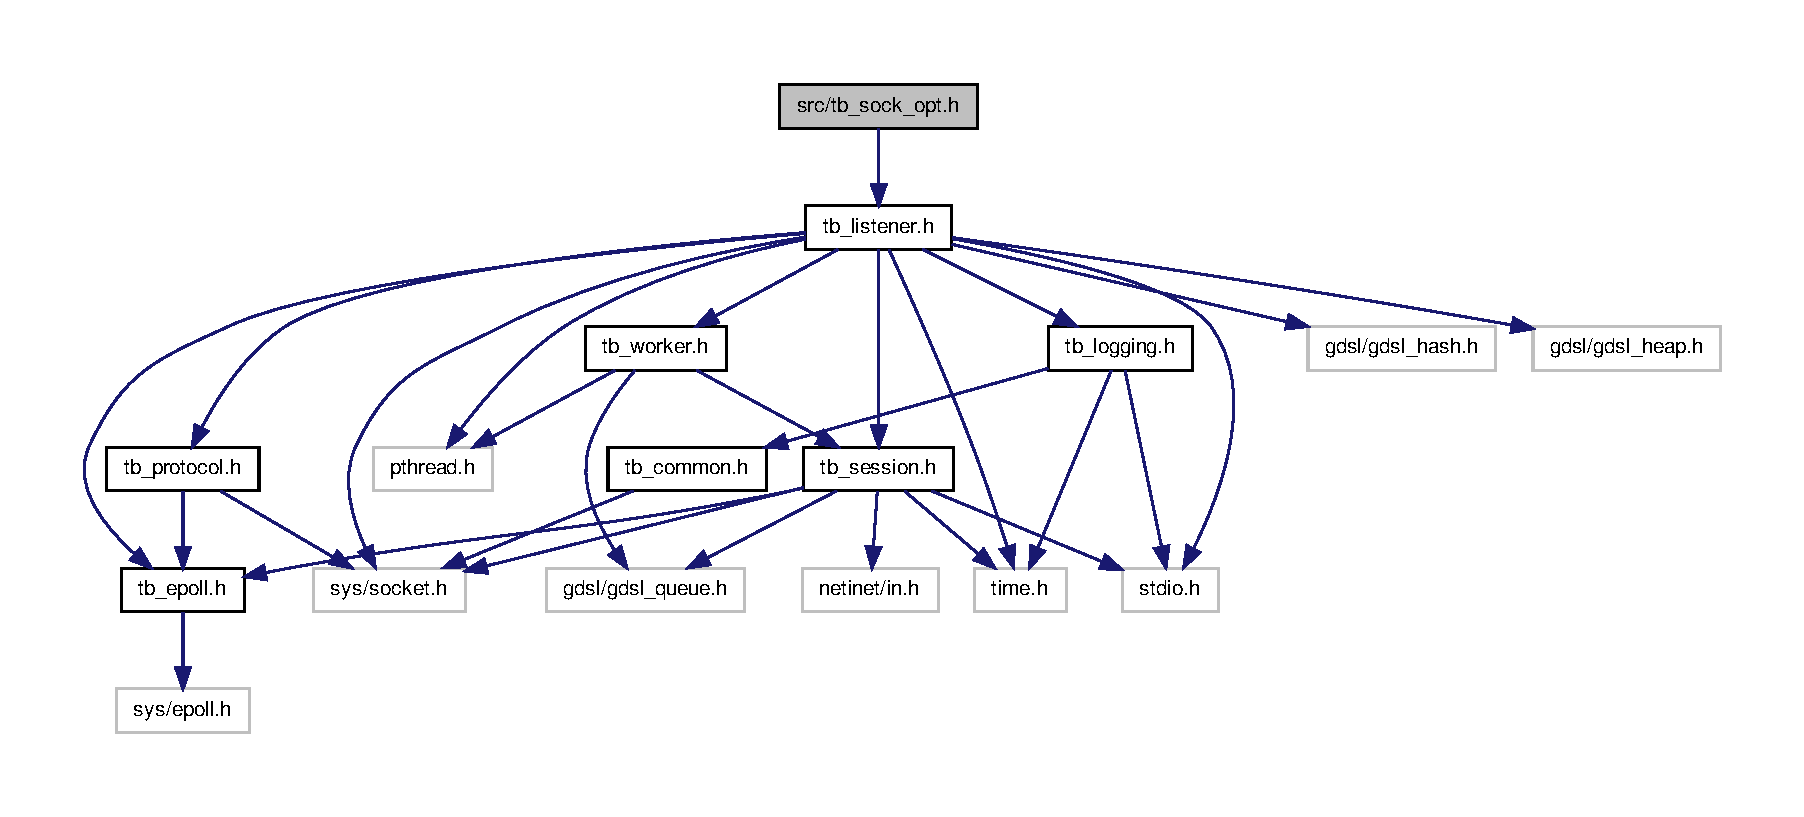
\includegraphics[width=350pt]{tb__sock__opt_8h__incl}
\end{center}
\end{figure}
This graph shows which files directly or indirectly include this file\-:\nopagebreak
\begin{figure}[H]
\begin{center}
\leavevmode
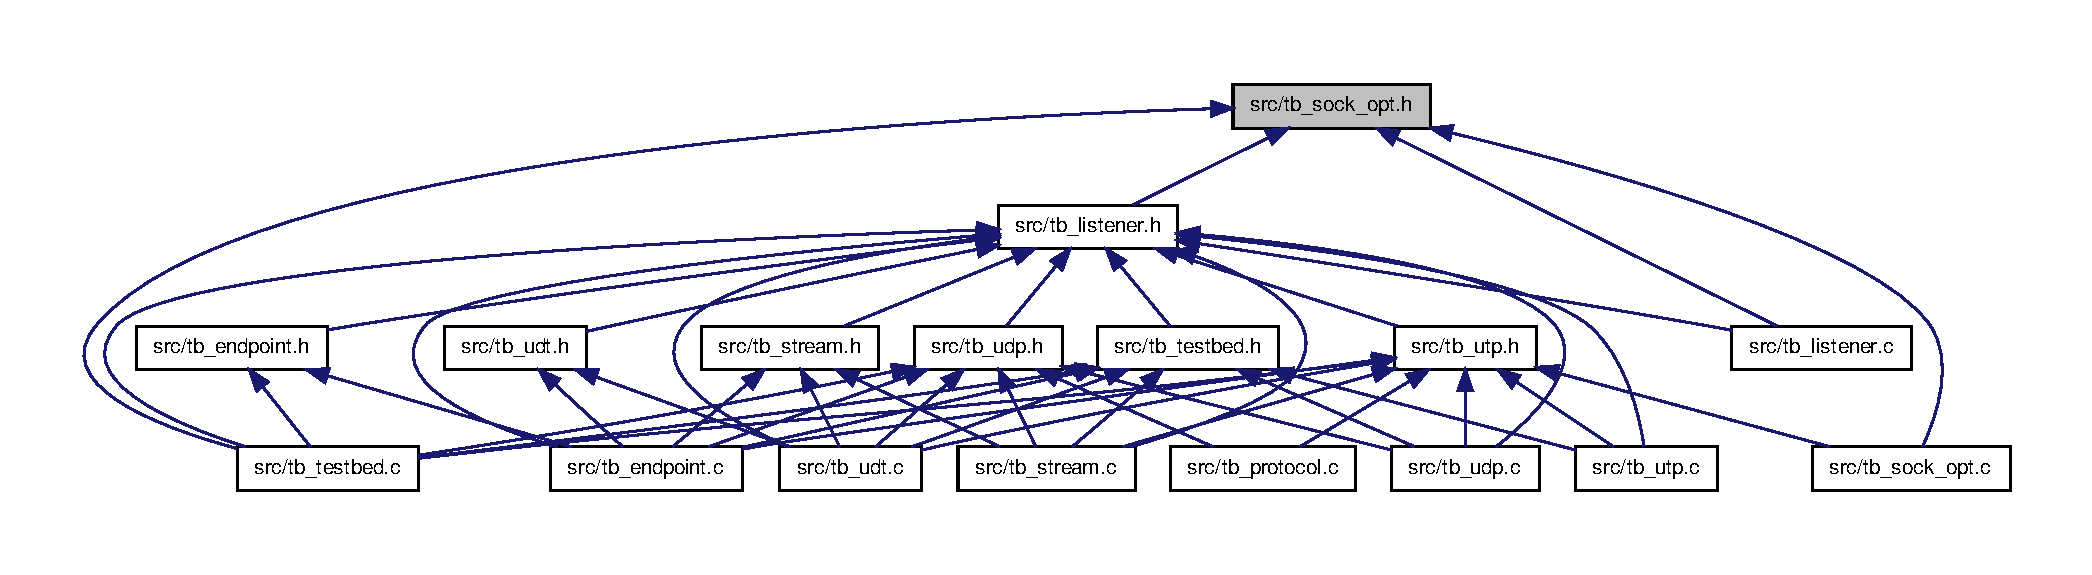
\includegraphics[width=350pt]{tb__sock__opt_8h__dep__incl}
\end{center}
\end{figure}
\subsection*{Data Structures}
\begin{DoxyCompactItemize}
\item 
struct \hyperlink{structtb__options__t}{tb\-\_\-options\-\_\-t}
\end{DoxyCompactItemize}
\subsection*{Functions}
\begin{DoxyCompactItemize}
\item 
int \hyperlink{tb__sock__opt_8h_a43b2b5e868cfb51f3e8ad367d8f354e8}{tb\-\_\-set\-\_\-sock\-\_\-opt} (\hyperlink{structtb__options__t}{tb\-\_\-options\-\_\-t} $\ast$options, int fd)
\begin{DoxyCompactList}\small\item\em Set options for individual protocols. \end{DoxyCompactList}\item 
int \hyperlink{tb__sock__opt_8h_aeb90bdb9face6f1bbe2e7c141a428cdf}{tb\-\_\-set\-\_\-bsd\-\_\-sock\-\_\-opts} (\hyperlink{structtb__options__t}{tb\-\_\-options\-\_\-t} $\ast$options, int fd)
\begin{DoxyCompactList}\small\item\em Set options for B\-S\-D sockets. Used by T\-C\-P, U\-D\-P and e\-U\-D\-P. \end{DoxyCompactList}\item 
int \hyperlink{tb__sock__opt_8h_a0c80d1c0e50d1312798c17f7f1add6e2}{tb\-\_\-set\-\_\-tcp\-\_\-opts} (\hyperlink{structtb__options__t}{tb\-\_\-options\-\_\-t} $\ast$options, int fd)
\begin{DoxyCompactList}\small\item\em Set options for T\-C\-P. \end{DoxyCompactList}\item 
int \hyperlink{tb__sock__opt_8h_af776cbfef331b9154f4cb40888e75bae}{tb\-\_\-set\-\_\-udp\-\_\-opts} (\hyperlink{structtb__options__t}{tb\-\_\-options\-\_\-t} $\ast$options, int fd)
\begin{DoxyCompactList}\small\item\em Set options for U\-D\-P. \end{DoxyCompactList}\item 
int \hyperlink{tb__sock__opt_8h_a834ce1097c65130cf74f1695eff08b1c}{tb\-\_\-set\-\_\-udt\-\_\-opts} (\hyperlink{structtb__options__t}{tb\-\_\-options\-\_\-t} $\ast$options, int fd)
\begin{DoxyCompactList}\small\item\em Set options for U\-D\-T. \end{DoxyCompactList}\item 
int \hyperlink{tb__sock__opt_8h_a178a04119b0fa7767e32fe915832c33e}{tb\-\_\-set\-\_\-audt\-\_\-opts} (\hyperlink{structtb__options__t}{tb\-\_\-options\-\_\-t} $\ast$options, int fd)
\begin{DoxyCompactList}\small\item\em Set options for a\-U\-D\-T. \end{DoxyCompactList}\item 
int \hyperlink{tb__sock__opt_8h_ac991c8bf8191d0900eac41096eeb3ab9}{tb\-\_\-set\-\_\-utp\-\_\-opts} (\hyperlink{structtb__options__t}{tb\-\_\-options\-\_\-t} $\ast$options, int fd)
\begin{DoxyCompactList}\small\item\em Set options for u\-T\-P. \end{DoxyCompactList}\item 
int \hyperlink{tb__sock__opt_8h_a3e68a727c2d788a487f8a973aec788f2}{tb\-\_\-set\-\_\-eudp\-\_\-opts} (\hyperlink{structtb__options__t}{tb\-\_\-options\-\_\-t} $\ast$options, int fd)
\begin{DoxyCompactList}\small\item\em Set options for e\-U\-D\-P. \end{DoxyCompactList}\item 
int \hyperlink{tb__sock__opt_8h_a1740be02ba9a1f9372be0ac2b4061f99}{tb\-\_\-set\-\_\-dccp\-\_\-opts} (\hyperlink{structtb__options__t}{tb\-\_\-options\-\_\-t} $\ast$options, int fd)
\begin{DoxyCompactList}\small\item\em Set options for D\-C\-C\-P. \end{DoxyCompactList}\end{DoxyCompactItemize}


\subsection{Function Documentation}
\hypertarget{tb__sock__opt_8h_a178a04119b0fa7767e32fe915832c33e}{\index{tb\-\_\-sock\-\_\-opt.\-h@{tb\-\_\-sock\-\_\-opt.\-h}!tb\-\_\-set\-\_\-audt\-\_\-opts@{tb\-\_\-set\-\_\-audt\-\_\-opts}}
\index{tb\-\_\-set\-\_\-audt\-\_\-opts@{tb\-\_\-set\-\_\-audt\-\_\-opts}!tb_sock_opt.h@{tb\-\_\-sock\-\_\-opt.\-h}}
\subsubsection[{tb\-\_\-set\-\_\-audt\-\_\-opts}]{\setlength{\rightskip}{0pt plus 5cm}int tb\-\_\-set\-\_\-audt\-\_\-opts (
\begin{DoxyParamCaption}
\item[{{\bf tb\-\_\-options\-\_\-t} $\ast$}]{options, }
\item[{int}]{fd}
\end{DoxyParamCaption}
)}}\label{tb__sock__opt_8h_a178a04119b0fa7767e32fe915832c33e}


Set options for a\-U\-D\-T. 



Definition at line 251 of file tb\-\_\-sock\-\_\-opt.\-c.

\hypertarget{tb__sock__opt_8h_aeb90bdb9face6f1bbe2e7c141a428cdf}{\index{tb\-\_\-sock\-\_\-opt.\-h@{tb\-\_\-sock\-\_\-opt.\-h}!tb\-\_\-set\-\_\-bsd\-\_\-sock\-\_\-opts@{tb\-\_\-set\-\_\-bsd\-\_\-sock\-\_\-opts}}
\index{tb\-\_\-set\-\_\-bsd\-\_\-sock\-\_\-opts@{tb\-\_\-set\-\_\-bsd\-\_\-sock\-\_\-opts}!tb_sock_opt.h@{tb\-\_\-sock\-\_\-opt.\-h}}
\subsubsection[{tb\-\_\-set\-\_\-bsd\-\_\-sock\-\_\-opts}]{\setlength{\rightskip}{0pt plus 5cm}int tb\-\_\-set\-\_\-bsd\-\_\-sock\-\_\-opts (
\begin{DoxyParamCaption}
\item[{{\bf tb\-\_\-options\-\_\-t} $\ast$}]{options, }
\item[{int}]{fd}
\end{DoxyParamCaption}
)}}\label{tb__sock__opt_8h_aeb90bdb9face6f1bbe2e7c141a428cdf}


Set options for B\-S\-D sockets. Used by T\-C\-P, U\-D\-P and e\-U\-D\-P. 



Definition at line 87 of file tb\-\_\-sock\-\_\-opt.\-c.

\hypertarget{tb__sock__opt_8h_a1740be02ba9a1f9372be0ac2b4061f99}{\index{tb\-\_\-sock\-\_\-opt.\-h@{tb\-\_\-sock\-\_\-opt.\-h}!tb\-\_\-set\-\_\-dccp\-\_\-opts@{tb\-\_\-set\-\_\-dccp\-\_\-opts}}
\index{tb\-\_\-set\-\_\-dccp\-\_\-opts@{tb\-\_\-set\-\_\-dccp\-\_\-opts}!tb_sock_opt.h@{tb\-\_\-sock\-\_\-opt.\-h}}
\subsubsection[{tb\-\_\-set\-\_\-dccp\-\_\-opts}]{\setlength{\rightskip}{0pt plus 5cm}int tb\-\_\-set\-\_\-dccp\-\_\-opts (
\begin{DoxyParamCaption}
\item[{{\bf tb\-\_\-options\-\_\-t} $\ast$}]{options, }
\item[{int}]{fd}
\end{DoxyParamCaption}
)}}\label{tb__sock__opt_8h_a1740be02ba9a1f9372be0ac2b4061f99}


Set options for D\-C\-C\-P. 



Definition at line 294 of file tb\-\_\-sock\-\_\-opt.\-c.

\hypertarget{tb__sock__opt_8h_a3e68a727c2d788a487f8a973aec788f2}{\index{tb\-\_\-sock\-\_\-opt.\-h@{tb\-\_\-sock\-\_\-opt.\-h}!tb\-\_\-set\-\_\-eudp\-\_\-opts@{tb\-\_\-set\-\_\-eudp\-\_\-opts}}
\index{tb\-\_\-set\-\_\-eudp\-\_\-opts@{tb\-\_\-set\-\_\-eudp\-\_\-opts}!tb_sock_opt.h@{tb\-\_\-sock\-\_\-opt.\-h}}
\subsubsection[{tb\-\_\-set\-\_\-eudp\-\_\-opts}]{\setlength{\rightskip}{0pt plus 5cm}int tb\-\_\-set\-\_\-eudp\-\_\-opts (
\begin{DoxyParamCaption}
\item[{{\bf tb\-\_\-options\-\_\-t} $\ast$}]{options, }
\item[{int}]{fd}
\end{DoxyParamCaption}
)}}\label{tb__sock__opt_8h_a3e68a727c2d788a487f8a973aec788f2}


Set options for e\-U\-D\-P. 



Definition at line 286 of file tb\-\_\-sock\-\_\-opt.\-c.

\hypertarget{tb__sock__opt_8h_a43b2b5e868cfb51f3e8ad367d8f354e8}{\index{tb\-\_\-sock\-\_\-opt.\-h@{tb\-\_\-sock\-\_\-opt.\-h}!tb\-\_\-set\-\_\-sock\-\_\-opt@{tb\-\_\-set\-\_\-sock\-\_\-opt}}
\index{tb\-\_\-set\-\_\-sock\-\_\-opt@{tb\-\_\-set\-\_\-sock\-\_\-opt}!tb_sock_opt.h@{tb\-\_\-sock\-\_\-opt.\-h}}
\subsubsection[{tb\-\_\-set\-\_\-sock\-\_\-opt}]{\setlength{\rightskip}{0pt plus 5cm}int tb\-\_\-set\-\_\-sock\-\_\-opt (
\begin{DoxyParamCaption}
\item[{{\bf tb\-\_\-options\-\_\-t} $\ast$}]{options, }
\item[{int}]{fd}
\end{DoxyParamCaption}
)}}\label{tb__sock__opt_8h_a43b2b5e868cfb51f3e8ad367d8f354e8}


Set options for individual protocols. 

This function is used to set the options on the currently used protocol.


\begin{DoxyParams}{Parameters}
{\em listener} & The currently used listener.\\
\hline
\end{DoxyParams}
\begin{DoxyReturn}{Returns}
0 if options were set, -\/1 otherwise. 
\end{DoxyReturn}


Definition at line 43 of file tb\-\_\-sock\-\_\-opt.\-c.

\hypertarget{tb__sock__opt_8h_a0c80d1c0e50d1312798c17f7f1add6e2}{\index{tb\-\_\-sock\-\_\-opt.\-h@{tb\-\_\-sock\-\_\-opt.\-h}!tb\-\_\-set\-\_\-tcp\-\_\-opts@{tb\-\_\-set\-\_\-tcp\-\_\-opts}}
\index{tb\-\_\-set\-\_\-tcp\-\_\-opts@{tb\-\_\-set\-\_\-tcp\-\_\-opts}!tb_sock_opt.h@{tb\-\_\-sock\-\_\-opt.\-h}}
\subsubsection[{tb\-\_\-set\-\_\-tcp\-\_\-opts}]{\setlength{\rightskip}{0pt plus 5cm}int tb\-\_\-set\-\_\-tcp\-\_\-opts (
\begin{DoxyParamCaption}
\item[{{\bf tb\-\_\-options\-\_\-t} $\ast$}]{options, }
\item[{int}]{fd}
\end{DoxyParamCaption}
)}}\label{tb__sock__opt_8h_a0c80d1c0e50d1312798c17f7f1add6e2}


Set options for T\-C\-P. 



Definition at line 133 of file tb\-\_\-sock\-\_\-opt.\-c.

\hypertarget{tb__sock__opt_8h_af776cbfef331b9154f4cb40888e75bae}{\index{tb\-\_\-sock\-\_\-opt.\-h@{tb\-\_\-sock\-\_\-opt.\-h}!tb\-\_\-set\-\_\-udp\-\_\-opts@{tb\-\_\-set\-\_\-udp\-\_\-opts}}
\index{tb\-\_\-set\-\_\-udp\-\_\-opts@{tb\-\_\-set\-\_\-udp\-\_\-opts}!tb_sock_opt.h@{tb\-\_\-sock\-\_\-opt.\-h}}
\subsubsection[{tb\-\_\-set\-\_\-udp\-\_\-opts}]{\setlength{\rightskip}{0pt plus 5cm}int tb\-\_\-set\-\_\-udp\-\_\-opts (
\begin{DoxyParamCaption}
\item[{{\bf tb\-\_\-options\-\_\-t} $\ast$}]{options, }
\item[{int}]{fd}
\end{DoxyParamCaption}
)}}\label{tb__sock__opt_8h_af776cbfef331b9154f4cb40888e75bae}


Set options for U\-D\-P. 



Definition at line 151 of file tb\-\_\-sock\-\_\-opt.\-c.

\hypertarget{tb__sock__opt_8h_a834ce1097c65130cf74f1695eff08b1c}{\index{tb\-\_\-sock\-\_\-opt.\-h@{tb\-\_\-sock\-\_\-opt.\-h}!tb\-\_\-set\-\_\-udt\-\_\-opts@{tb\-\_\-set\-\_\-udt\-\_\-opts}}
\index{tb\-\_\-set\-\_\-udt\-\_\-opts@{tb\-\_\-set\-\_\-udt\-\_\-opts}!tb_sock_opt.h@{tb\-\_\-sock\-\_\-opt.\-h}}
\subsubsection[{tb\-\_\-set\-\_\-udt\-\_\-opts}]{\setlength{\rightskip}{0pt plus 5cm}int tb\-\_\-set\-\_\-udt\-\_\-opts (
\begin{DoxyParamCaption}
\item[{{\bf tb\-\_\-options\-\_\-t} $\ast$}]{options, }
\item[{int}]{fd}
\end{DoxyParamCaption}
)}}\label{tb__sock__opt_8h_a834ce1097c65130cf74f1695eff08b1c}


Set options for U\-D\-T. 



Definition at line 171 of file tb\-\_\-sock\-\_\-opt.\-c.

\hypertarget{tb__sock__opt_8h_ac991c8bf8191d0900eac41096eeb3ab9}{\index{tb\-\_\-sock\-\_\-opt.\-h@{tb\-\_\-sock\-\_\-opt.\-h}!tb\-\_\-set\-\_\-utp\-\_\-opts@{tb\-\_\-set\-\_\-utp\-\_\-opts}}
\index{tb\-\_\-set\-\_\-utp\-\_\-opts@{tb\-\_\-set\-\_\-utp\-\_\-opts}!tb_sock_opt.h@{tb\-\_\-sock\-\_\-opt.\-h}}
\subsubsection[{tb\-\_\-set\-\_\-utp\-\_\-opts}]{\setlength{\rightskip}{0pt plus 5cm}int tb\-\_\-set\-\_\-utp\-\_\-opts (
\begin{DoxyParamCaption}
\item[{{\bf tb\-\_\-options\-\_\-t} $\ast$}]{options, }
\item[{int}]{fd}
\end{DoxyParamCaption}
)}}\label{tb__sock__opt_8h_ac991c8bf8191d0900eac41096eeb3ab9}


Set options for u\-T\-P. 



Definition at line 257 of file tb\-\_\-sock\-\_\-opt.\-c.


\hypertarget{tb__stream_8c}{\section{src/tb\-\_\-stream.c File Reference}
\label{tb__stream_8c}\index{src/tb\-\_\-stream.\-c@{src/tb\-\_\-stream.\-c}}
}
{\ttfamily \#include \char`\"{}tb\-\_\-stream.\-h\char`\"{}}\\*
{\ttfamily \#include \char`\"{}tb\-\_\-protocol.\-h\char`\"{}}\\*
{\ttfamily \#include \char`\"{}tb\-\_\-listener.\-h\char`\"{}}\\*
{\ttfamily \#include \char`\"{}tb\-\_\-testbed.\-h\char`\"{}}\\*
{\ttfamily \#include \char`\"{}tb\-\_\-common.\-h\char`\"{}}\\*
{\ttfamily \#include \char`\"{}tb\-\_\-udp.\-h\char`\"{}}\\*
{\ttfamily \#include \char`\"{}tb\-\_\-utp.\-h\char`\"{}}\\*
{\ttfamily \#include \char`\"{}udt.\-h\char`\"{}}\\*
{\ttfamily \#include \char`\"{}tb\-\_\-session.\-h\char`\"{}}\\*
{\ttfamily \#include $<$utp.\-h$>$}\\*
{\ttfamily \#include $<$stdio.\-h$>$}\\*
{\ttfamily \#include $<$stdlib.\-h$>$}\\*
{\ttfamily \#include $<$assert.\-h$>$}\\*
{\ttfamily \#include $<$pthread.\-h$>$}\\*
{\ttfamily \#include $<$sys/socket.\-h$>$}\\*
{\ttfamily \#include $<$fcntl.\-h$>$}\\*
{\ttfamily \#include $<$unistd.\-h$>$}\\*
{\ttfamily \#include $<$string.\-h$>$}\\*
{\ttfamily \#include $<$sys/epoll.\-h$>$}\\*
{\ttfamily \#include $<$time.\-h$>$}\\*
{\ttfamily \#include $<$errno.\-h$>$}\\*
Include dependency graph for tb\-\_\-stream.\-c\-:\nopagebreak
\begin{figure}[H]
\begin{center}
\leavevmode
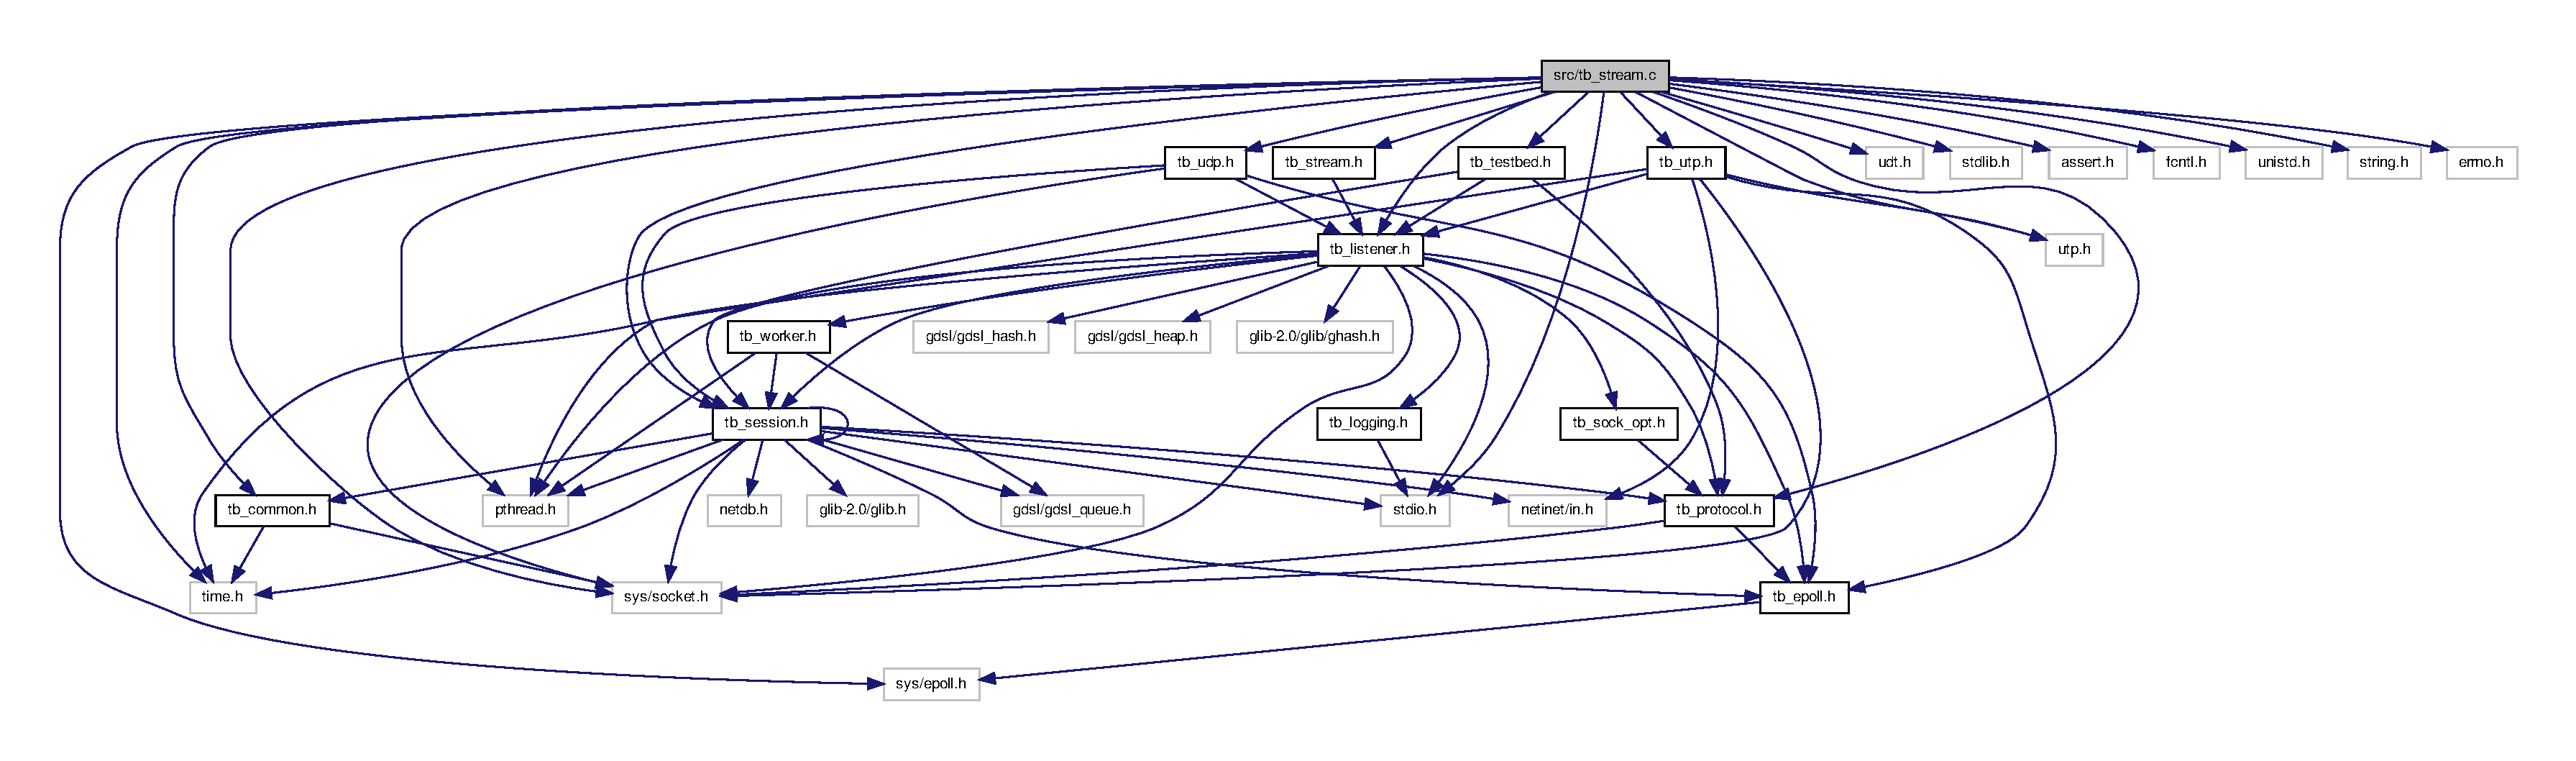
\includegraphics[width=350pt]{tb__stream_8c__incl}
\end{center}
\end{figure}
\subsection*{Functions}
\begin{DoxyCompactItemize}
\item 
int \hyperlink{tb__stream_8c_ab254f51747c78bfc75e1dd91945936af}{tb\-\_\-stream\-\_\-server} (\hyperlink{structtb__listener__t}{tb\-\_\-listener\-\_\-t} $\ast$listener)
\begin{DoxyCompactList}\small\item\em Run a server without epoll (blocking socket). \end{DoxyCompactList}\item 
int \hyperlink{tb__stream_8c_a736ead28c313623ab95be2738fa6a2d8}{tb\-\_\-stream\-\_\-m\-\_\-server} (\hyperlink{structtb__listener__t}{tb\-\_\-listener\-\_\-t} $\ast$listener)
\begin{DoxyCompactList}\small\item\em Run a multiple connection server. \end{DoxyCompactList}\item 
int \hyperlink{tb__stream_8c_a2824c0d70d74f26a227971550f32446f}{tb\-\_\-stream\-\_\-event} (int events, void $\ast$data)
\begin{DoxyCompactList}\small\item\em Called by epoll. \end{DoxyCompactList}\item 
void $\ast$ \hyperlink{tb__stream_8c_afbdad677cb3cfe90954ec6e482fec19c}{tb\-\_\-stream\-\_\-m\-\_\-server\-\_\-conn} (void $\ast$data)
\begin{DoxyCompactList}\small\item\em Individual stream connections for multiple stream servers. \end{DoxyCompactList}\item 
int \hyperlink{tb__stream_8c_a4836f7e8e6b482f36a354d52d16b5843}{tb\-\_\-stream\-\_\-m\-\_\-client} (\hyperlink{structtb__listener__t}{tb\-\_\-listener\-\_\-t} $\ast$listener)
\begin{DoxyCompactList}\small\item\em Upload using stream sockets. \end{DoxyCompactList}\item 
void $\ast$ \hyperlink{tb__stream_8c_aaa8373bc3d9d810fb73ce3cf09dbd27a}{tb\-\_\-stream\-\_\-connection} (void $\ast$data)
\begin{DoxyCompactList}\small\item\em A single stream connection. \end{DoxyCompactList}\item 
int \hyperlink{tb__stream_8c_a37207d097b0a8f4906fda05c22b5d851}{tb\-\_\-stream\-\_\-client} (\hyperlink{structtb__listener__t}{tb\-\_\-listener\-\_\-t} $\ast$listener)
\begin{DoxyCompactList}\small\item\em Upload with a single connection. \end{DoxyCompactList}\end{DoxyCompactItemize}


\subsection{Function Documentation}
\hypertarget{tb__stream_8c_a37207d097b0a8f4906fda05c22b5d851}{\index{tb\-\_\-stream.\-c@{tb\-\_\-stream.\-c}!tb\-\_\-stream\-\_\-client@{tb\-\_\-stream\-\_\-client}}
\index{tb\-\_\-stream\-\_\-client@{tb\-\_\-stream\-\_\-client}!tb_stream.c@{tb\-\_\-stream.\-c}}
\subsubsection[{tb\-\_\-stream\-\_\-client}]{\setlength{\rightskip}{0pt plus 5cm}int tb\-\_\-stream\-\_\-client (
\begin{DoxyParamCaption}
\item[{{\bf tb\-\_\-listener\-\_\-t} $\ast$}]{listener}
\end{DoxyParamCaption}
)}}\label{tb__stream_8c_a37207d097b0a8f4906fda05c22b5d851}


Upload with a single connection. 



Definition at line 370 of file tb\-\_\-stream.\-c.

\hypertarget{tb__stream_8c_aaa8373bc3d9d810fb73ce3cf09dbd27a}{\index{tb\-\_\-stream.\-c@{tb\-\_\-stream.\-c}!tb\-\_\-stream\-\_\-connection@{tb\-\_\-stream\-\_\-connection}}
\index{tb\-\_\-stream\-\_\-connection@{tb\-\_\-stream\-\_\-connection}!tb_stream.c@{tb\-\_\-stream.\-c}}
\subsubsection[{tb\-\_\-stream\-\_\-connection}]{\setlength{\rightskip}{0pt plus 5cm}void$\ast$ tb\-\_\-stream\-\_\-connection (
\begin{DoxyParamCaption}
\item[{void $\ast$}]{data}
\end{DoxyParamCaption}
)}}\label{tb__stream_8c_aaa8373bc3d9d810fb73ce3cf09dbd27a}


A single stream connection. 



Definition at line 312 of file tb\-\_\-stream.\-c.

\hypertarget{tb__stream_8c_a2824c0d70d74f26a227971550f32446f}{\index{tb\-\_\-stream.\-c@{tb\-\_\-stream.\-c}!tb\-\_\-stream\-\_\-event@{tb\-\_\-stream\-\_\-event}}
\index{tb\-\_\-stream\-\_\-event@{tb\-\_\-stream\-\_\-event}!tb_stream.c@{tb\-\_\-stream.\-c}}
\subsubsection[{tb\-\_\-stream\-\_\-event}]{\setlength{\rightskip}{0pt plus 5cm}int tb\-\_\-stream\-\_\-event (
\begin{DoxyParamCaption}
\item[{int}]{events, }
\item[{void $\ast$}]{data}
\end{DoxyParamCaption}
)}}\label{tb__stream_8c_a2824c0d70d74f26a227971550f32446f}


Called by epoll. 



Definition at line 123 of file tb\-\_\-stream.\-c.

\hypertarget{tb__stream_8c_a4836f7e8e6b482f36a354d52d16b5843}{\index{tb\-\_\-stream.\-c@{tb\-\_\-stream.\-c}!tb\-\_\-stream\-\_\-m\-\_\-client@{tb\-\_\-stream\-\_\-m\-\_\-client}}
\index{tb\-\_\-stream\-\_\-m\-\_\-client@{tb\-\_\-stream\-\_\-m\-\_\-client}!tb_stream.c@{tb\-\_\-stream.\-c}}
\subsubsection[{tb\-\_\-stream\-\_\-m\-\_\-client}]{\setlength{\rightskip}{0pt plus 5cm}int tb\-\_\-stream\-\_\-m\-\_\-client (
\begin{DoxyParamCaption}
\item[{{\bf tb\-\_\-listener\-\_\-t} $\ast$}]{listener}
\end{DoxyParamCaption}
)}}\label{tb__stream_8c_a4836f7e8e6b482f36a354d52d16b5843}


Upload using stream sockets. 

Upload using bsd stream based protocols (T\-C\-P, D\-C\-C\-P) with multiple connections. 

Definition at line 222 of file tb\-\_\-stream.\-c.

\hypertarget{tb__stream_8c_a736ead28c313623ab95be2738fa6a2d8}{\index{tb\-\_\-stream.\-c@{tb\-\_\-stream.\-c}!tb\-\_\-stream\-\_\-m\-\_\-server@{tb\-\_\-stream\-\_\-m\-\_\-server}}
\index{tb\-\_\-stream\-\_\-m\-\_\-server@{tb\-\_\-stream\-\_\-m\-\_\-server}!tb_stream.c@{tb\-\_\-stream.\-c}}
\subsubsection[{tb\-\_\-stream\-\_\-m\-\_\-server}]{\setlength{\rightskip}{0pt plus 5cm}int tb\-\_\-stream\-\_\-m\-\_\-server (
\begin{DoxyParamCaption}
\item[{{\bf tb\-\_\-listener\-\_\-t} $\ast$}]{listener}
\end{DoxyParamCaption}
)}}\label{tb__stream_8c_a736ead28c313623ab95be2738fa6a2d8}


Run a multiple connection server. 


\begin{DoxyParams}{Parameters}
{\em listener} & The listener to create the server for \\
\hline
\end{DoxyParams}


Definition at line 106 of file tb\-\_\-stream.\-c.

\hypertarget{tb__stream_8c_afbdad677cb3cfe90954ec6e482fec19c}{\index{tb\-\_\-stream.\-c@{tb\-\_\-stream.\-c}!tb\-\_\-stream\-\_\-m\-\_\-server\-\_\-conn@{tb\-\_\-stream\-\_\-m\-\_\-server\-\_\-conn}}
\index{tb\-\_\-stream\-\_\-m\-\_\-server\-\_\-conn@{tb\-\_\-stream\-\_\-m\-\_\-server\-\_\-conn}!tb_stream.c@{tb\-\_\-stream.\-c}}
\subsubsection[{tb\-\_\-stream\-\_\-m\-\_\-server\-\_\-conn}]{\setlength{\rightskip}{0pt plus 5cm}void$\ast$ tb\-\_\-stream\-\_\-m\-\_\-server\-\_\-conn (
\begin{DoxyParamCaption}
\item[{void $\ast$}]{data}
\end{DoxyParamCaption}
)}}\label{tb__stream_8c_afbdad677cb3cfe90954ec6e482fec19c}


Individual stream connections for multiple stream servers. 



Definition at line 175 of file tb\-\_\-stream.\-c.

\hypertarget{tb__stream_8c_ab254f51747c78bfc75e1dd91945936af}{\index{tb\-\_\-stream.\-c@{tb\-\_\-stream.\-c}!tb\-\_\-stream\-\_\-server@{tb\-\_\-stream\-\_\-server}}
\index{tb\-\_\-stream\-\_\-server@{tb\-\_\-stream\-\_\-server}!tb_stream.c@{tb\-\_\-stream.\-c}}
\subsubsection[{tb\-\_\-stream\-\_\-server}]{\setlength{\rightskip}{0pt plus 5cm}int tb\-\_\-stream\-\_\-server (
\begin{DoxyParamCaption}
\item[{{\bf tb\-\_\-listener\-\_\-t} $\ast$}]{listener}
\end{DoxyParamCaption}
)}}\label{tb__stream_8c_ab254f51747c78bfc75e1dd91945936af}


Run a server without epoll (blocking socket). 

Runs a server without using epoll, so the socket blocks. Also used by U\-D\-T, a\-U\-D\-T and other protocols that are not implemented in sockets.


\begin{DoxyParams}{Parameters}
{\em listener} & The listener to run the server with. \\
\hline
\end{DoxyParams}


Definition at line 36 of file tb\-\_\-stream.\-c.


\hypertarget{tb__stream_8h}{\section{src/tb\-\_\-stream.h File Reference}
\label{tb__stream_8h}\index{src/tb\-\_\-stream.\-h@{src/tb\-\_\-stream.\-h}}
}
{\ttfamily \#include \char`\"{}tb\-\_\-listener.\-h\char`\"{}}\\*
Include dependency graph for tb\-\_\-stream.\-h\-:\nopagebreak
\begin{figure}[H]
\begin{center}
\leavevmode
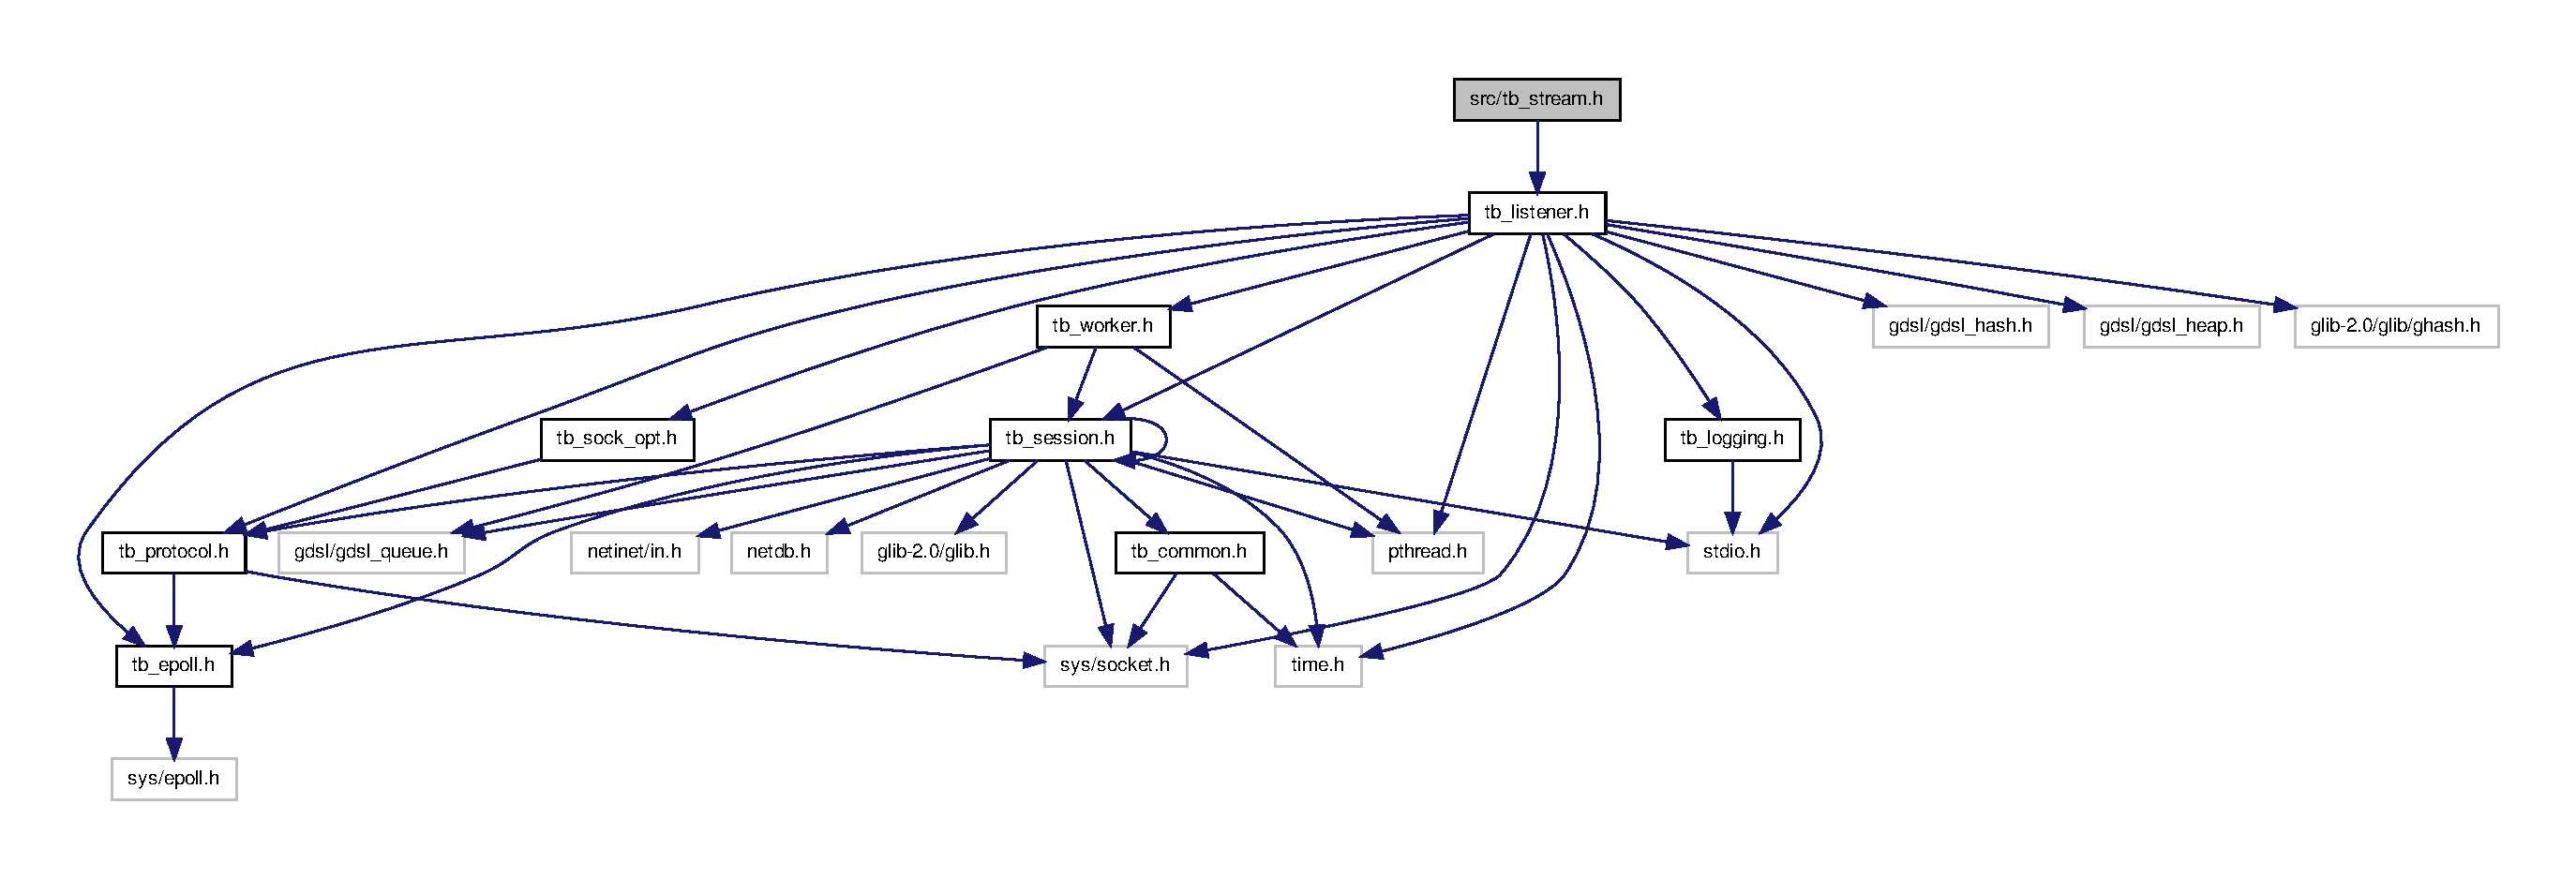
\includegraphics[width=350pt]{tb__stream_8h__incl}
\end{center}
\end{figure}
This graph shows which files directly or indirectly include this file\-:\nopagebreak
\begin{figure}[H]
\begin{center}
\leavevmode
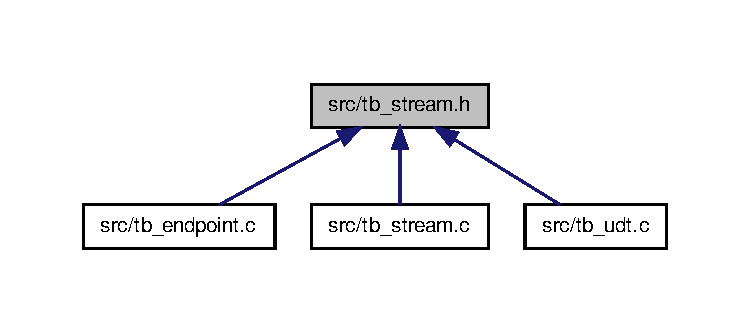
\includegraphics[width=350pt]{tb__stream_8h__dep__incl}
\end{center}
\end{figure}
\subsection*{Functions}
\begin{DoxyCompactItemize}
\item 
int \hyperlink{tb__stream_8h_ab254f51747c78bfc75e1dd91945936af}{tb\-\_\-stream\-\_\-server} (\hyperlink{structtb__listener__t}{tb\-\_\-listener\-\_\-t} $\ast$listener)
\begin{DoxyCompactList}\small\item\em Run a server without epoll (blocking socket). \end{DoxyCompactList}\item 
int \hyperlink{tb__stream_8h_a736ead28c313623ab95be2738fa6a2d8}{tb\-\_\-stream\-\_\-m\-\_\-server} (\hyperlink{structtb__listener__t}{tb\-\_\-listener\-\_\-t} $\ast$listener)
\begin{DoxyCompactList}\small\item\em Run a multiple connection server. \end{DoxyCompactList}\item 
int \hyperlink{tb__stream_8h_a2824c0d70d74f26a227971550f32446f}{tb\-\_\-stream\-\_\-event} (int events, void $\ast$data)
\begin{DoxyCompactList}\small\item\em Called by epoll. \end{DoxyCompactList}\item 
void $\ast$ \hyperlink{tb__stream_8h_afbdad677cb3cfe90954ec6e482fec19c}{tb\-\_\-stream\-\_\-m\-\_\-server\-\_\-conn} (void $\ast$data)
\begin{DoxyCompactList}\small\item\em Individual stream connections for multiple stream servers. \end{DoxyCompactList}\item 
int \hyperlink{tb__stream_8h_a4836f7e8e6b482f36a354d52d16b5843}{tb\-\_\-stream\-\_\-m\-\_\-client} (\hyperlink{structtb__listener__t}{tb\-\_\-listener\-\_\-t} $\ast$listener)
\begin{DoxyCompactList}\small\item\em Upload using stream sockets. \end{DoxyCompactList}\item 
void $\ast$ \hyperlink{tb__stream_8h_aaa8373bc3d9d810fb73ce3cf09dbd27a}{tb\-\_\-stream\-\_\-connection} (void $\ast$data)
\begin{DoxyCompactList}\small\item\em A single stream connection. \end{DoxyCompactList}\item 
int \hyperlink{tb__stream_8h_a37207d097b0a8f4906fda05c22b5d851}{tb\-\_\-stream\-\_\-client} (\hyperlink{structtb__listener__t}{tb\-\_\-listener\-\_\-t} $\ast$listener)
\begin{DoxyCompactList}\small\item\em Upload with a single connection. \end{DoxyCompactList}\end{DoxyCompactItemize}


\subsection{Function Documentation}
\hypertarget{tb__stream_8h_a37207d097b0a8f4906fda05c22b5d851}{\index{tb\-\_\-stream.\-h@{tb\-\_\-stream.\-h}!tb\-\_\-stream\-\_\-client@{tb\-\_\-stream\-\_\-client}}
\index{tb\-\_\-stream\-\_\-client@{tb\-\_\-stream\-\_\-client}!tb_stream.h@{tb\-\_\-stream.\-h}}
\subsubsection[{tb\-\_\-stream\-\_\-client}]{\setlength{\rightskip}{0pt plus 5cm}int tb\-\_\-stream\-\_\-client (
\begin{DoxyParamCaption}
\item[{{\bf tb\-\_\-listener\-\_\-t} $\ast$}]{listener}
\end{DoxyParamCaption}
)}}\label{tb__stream_8h_a37207d097b0a8f4906fda05c22b5d851}


Upload with a single connection. 



Definition at line 370 of file tb\-\_\-stream.\-c.

\hypertarget{tb__stream_8h_aaa8373bc3d9d810fb73ce3cf09dbd27a}{\index{tb\-\_\-stream.\-h@{tb\-\_\-stream.\-h}!tb\-\_\-stream\-\_\-connection@{tb\-\_\-stream\-\_\-connection}}
\index{tb\-\_\-stream\-\_\-connection@{tb\-\_\-stream\-\_\-connection}!tb_stream.h@{tb\-\_\-stream.\-h}}
\subsubsection[{tb\-\_\-stream\-\_\-connection}]{\setlength{\rightskip}{0pt plus 5cm}void$\ast$ tb\-\_\-stream\-\_\-connection (
\begin{DoxyParamCaption}
\item[{void $\ast$}]{data}
\end{DoxyParamCaption}
)}}\label{tb__stream_8h_aaa8373bc3d9d810fb73ce3cf09dbd27a}


A single stream connection. 



Definition at line 312 of file tb\-\_\-stream.\-c.

\hypertarget{tb__stream_8h_a2824c0d70d74f26a227971550f32446f}{\index{tb\-\_\-stream.\-h@{tb\-\_\-stream.\-h}!tb\-\_\-stream\-\_\-event@{tb\-\_\-stream\-\_\-event}}
\index{tb\-\_\-stream\-\_\-event@{tb\-\_\-stream\-\_\-event}!tb_stream.h@{tb\-\_\-stream.\-h}}
\subsubsection[{tb\-\_\-stream\-\_\-event}]{\setlength{\rightskip}{0pt plus 5cm}int tb\-\_\-stream\-\_\-event (
\begin{DoxyParamCaption}
\item[{int}]{events, }
\item[{void $\ast$}]{data}
\end{DoxyParamCaption}
)}}\label{tb__stream_8h_a2824c0d70d74f26a227971550f32446f}


Called by epoll. 



Definition at line 123 of file tb\-\_\-stream.\-c.

\hypertarget{tb__stream_8h_a4836f7e8e6b482f36a354d52d16b5843}{\index{tb\-\_\-stream.\-h@{tb\-\_\-stream.\-h}!tb\-\_\-stream\-\_\-m\-\_\-client@{tb\-\_\-stream\-\_\-m\-\_\-client}}
\index{tb\-\_\-stream\-\_\-m\-\_\-client@{tb\-\_\-stream\-\_\-m\-\_\-client}!tb_stream.h@{tb\-\_\-stream.\-h}}
\subsubsection[{tb\-\_\-stream\-\_\-m\-\_\-client}]{\setlength{\rightskip}{0pt plus 5cm}int tb\-\_\-stream\-\_\-m\-\_\-client (
\begin{DoxyParamCaption}
\item[{{\bf tb\-\_\-listener\-\_\-t} $\ast$}]{listener}
\end{DoxyParamCaption}
)}}\label{tb__stream_8h_a4836f7e8e6b482f36a354d52d16b5843}


Upload using stream sockets. 

Upload using bsd stream based protocols (T\-C\-P, D\-C\-C\-P) with multiple connections. 

Definition at line 222 of file tb\-\_\-stream.\-c.

\hypertarget{tb__stream_8h_a736ead28c313623ab95be2738fa6a2d8}{\index{tb\-\_\-stream.\-h@{tb\-\_\-stream.\-h}!tb\-\_\-stream\-\_\-m\-\_\-server@{tb\-\_\-stream\-\_\-m\-\_\-server}}
\index{tb\-\_\-stream\-\_\-m\-\_\-server@{tb\-\_\-stream\-\_\-m\-\_\-server}!tb_stream.h@{tb\-\_\-stream.\-h}}
\subsubsection[{tb\-\_\-stream\-\_\-m\-\_\-server}]{\setlength{\rightskip}{0pt plus 5cm}int tb\-\_\-stream\-\_\-m\-\_\-server (
\begin{DoxyParamCaption}
\item[{{\bf tb\-\_\-listener\-\_\-t} $\ast$}]{listener}
\end{DoxyParamCaption}
)}}\label{tb__stream_8h_a736ead28c313623ab95be2738fa6a2d8}


Run a multiple connection server. 


\begin{DoxyParams}{Parameters}
{\em listener} & The listener to create the server for \\
\hline
\end{DoxyParams}


Definition at line 106 of file tb\-\_\-stream.\-c.

\hypertarget{tb__stream_8h_afbdad677cb3cfe90954ec6e482fec19c}{\index{tb\-\_\-stream.\-h@{tb\-\_\-stream.\-h}!tb\-\_\-stream\-\_\-m\-\_\-server\-\_\-conn@{tb\-\_\-stream\-\_\-m\-\_\-server\-\_\-conn}}
\index{tb\-\_\-stream\-\_\-m\-\_\-server\-\_\-conn@{tb\-\_\-stream\-\_\-m\-\_\-server\-\_\-conn}!tb_stream.h@{tb\-\_\-stream.\-h}}
\subsubsection[{tb\-\_\-stream\-\_\-m\-\_\-server\-\_\-conn}]{\setlength{\rightskip}{0pt plus 5cm}void$\ast$ tb\-\_\-stream\-\_\-m\-\_\-server\-\_\-conn (
\begin{DoxyParamCaption}
\item[{void $\ast$}]{data}
\end{DoxyParamCaption}
)}}\label{tb__stream_8h_afbdad677cb3cfe90954ec6e482fec19c}


Individual stream connections for multiple stream servers. 



Definition at line 175 of file tb\-\_\-stream.\-c.

\hypertarget{tb__stream_8h_ab254f51747c78bfc75e1dd91945936af}{\index{tb\-\_\-stream.\-h@{tb\-\_\-stream.\-h}!tb\-\_\-stream\-\_\-server@{tb\-\_\-stream\-\_\-server}}
\index{tb\-\_\-stream\-\_\-server@{tb\-\_\-stream\-\_\-server}!tb_stream.h@{tb\-\_\-stream.\-h}}
\subsubsection[{tb\-\_\-stream\-\_\-server}]{\setlength{\rightskip}{0pt plus 5cm}int tb\-\_\-stream\-\_\-server (
\begin{DoxyParamCaption}
\item[{{\bf tb\-\_\-listener\-\_\-t} $\ast$}]{listener}
\end{DoxyParamCaption}
)}}\label{tb__stream_8h_ab254f51747c78bfc75e1dd91945936af}


Run a server without epoll (blocking socket). 

Runs a server without using epoll, so the socket blocks. Also used by U\-D\-T, a\-U\-D\-T and other protocols that are not implemented in sockets.


\begin{DoxyParams}{Parameters}
{\em listener} & The listener to run the server with. \\
\hline
\end{DoxyParams}


Definition at line 36 of file tb\-\_\-stream.\-c.


\hypertarget{tb__testbed_8c}{\section{src/tb\-\_\-testbed.c File Reference}
\label{tb__testbed_8c}\index{src/tb\-\_\-testbed.\-c@{src/tb\-\_\-testbed.\-c}}
}
{\ttfamily \#include \char`\"{}tb\-\_\-testbed.\-h\char`\"{}}\\*
{\ttfamily \#include \char`\"{}tb\-\_\-protocol.\-h\char`\"{}}\\*
{\ttfamily \#include \char`\"{}tb\-\_\-listener.\-h\char`\"{}}\\*
{\ttfamily \#include \char`\"{}tb\-\_\-session.\-h\char`\"{}}\\*
{\ttfamily \#include \char`\"{}tb\-\_\-common.\-h\char`\"{}}\\*
{\ttfamily \#include \char`\"{}tb\-\_\-utp.\-h\char`\"{}}\\*
{\ttfamily \#include \char`\"{}tb\-\_\-udp.\-h\char`\"{}}\\*
{\ttfamily \#include \char`\"{}tb\-\_\-sock\-\_\-opt.\-h\char`\"{}}\\*
{\ttfamily \#include \char`\"{}tb\-\_\-logging.\-h\char`\"{}}\\*
{\ttfamily \#include \char`\"{}tb\-\_\-endpoint.\-h\char`\"{}}\\*
{\ttfamily \#include $<$pthread.\-h$>$}\\*
{\ttfamily \#include $<$stdio.\-h$>$}\\*
{\ttfamily \#include $<$stdlib.\-h$>$}\\*
{\ttfamily \#include $<$assert.\-h$>$}\\*
{\ttfamily \#include $<$sys/socket.\-h$>$}\\*
{\ttfamily \#include $<$fcntl.\-h$>$}\\*
{\ttfamily \#include $<$unistd.\-h$>$}\\*
{\ttfamily \#include $<$string.\-h$>$}\\*
{\ttfamily \#include $<$sys/epoll.\-h$>$}\\*
{\ttfamily \#include $<$time.\-h$>$}\\*
{\ttfamily \#include $<$signal.\-h$>$}\\*
{\ttfamily \#include $<$sched.\-h$>$}\\*
{\ttfamily \#include $<$netdb.\-h$>$}\\*
{\ttfamily \#include $<$errno.\-h$>$}\\*
Include dependency graph for tb\-\_\-testbed.\-c\-:\nopagebreak
\begin{figure}[H]
\begin{center}
\leavevmode
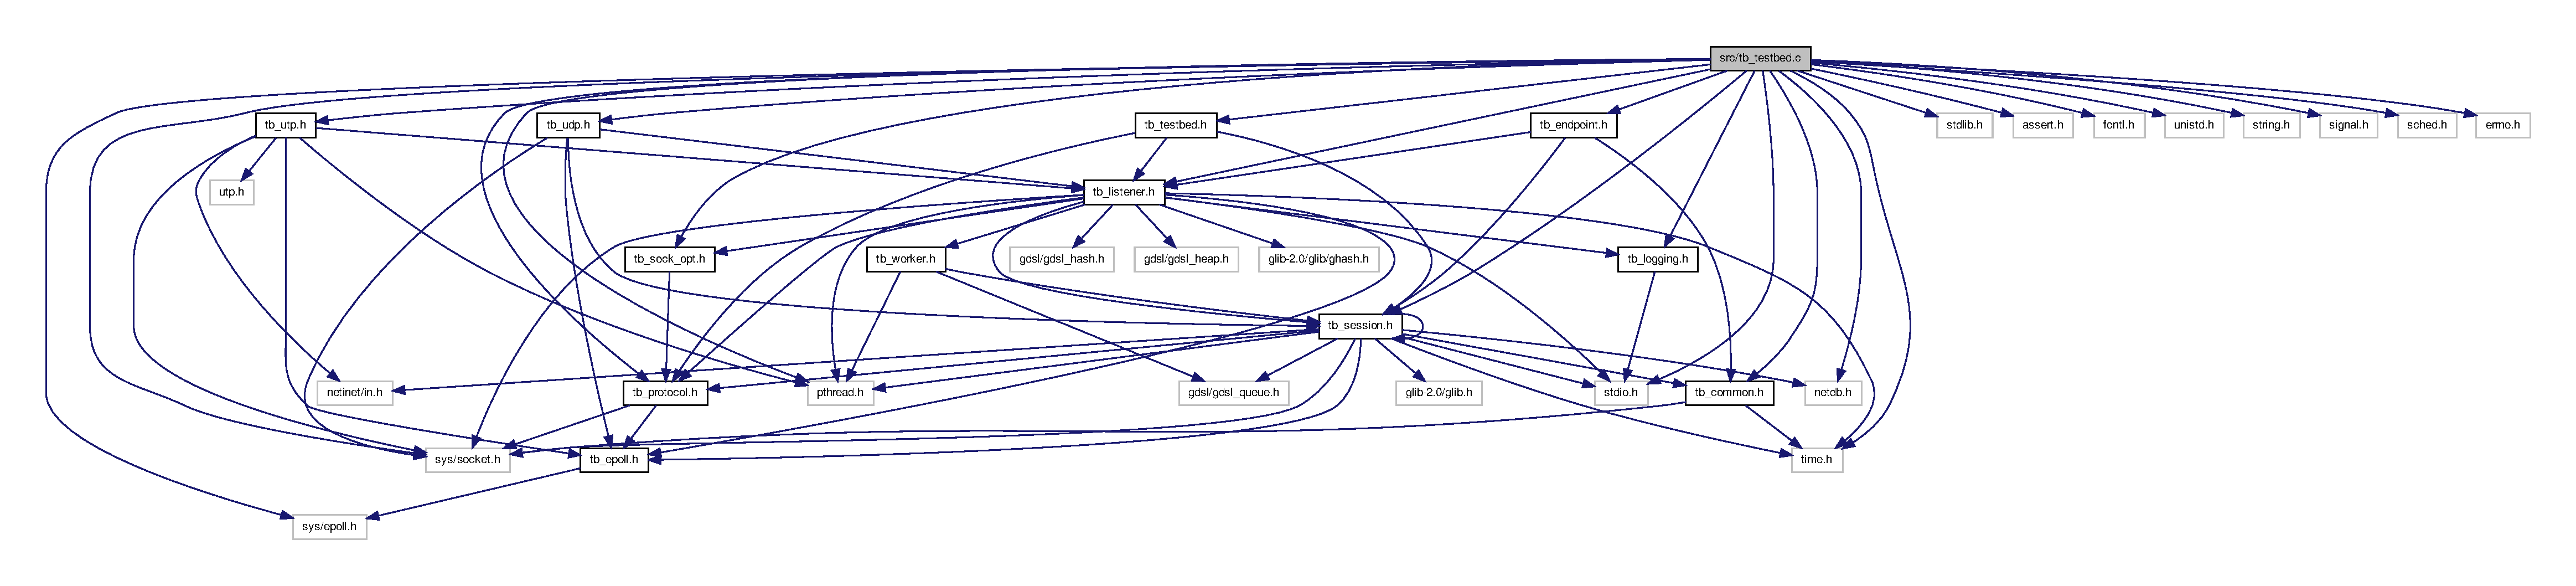
\includegraphics[width=350pt]{tb__testbed_8c__incl}
\end{center}
\end{figure}
\subsection*{Functions}
\begin{DoxyCompactItemize}
\item 
int \hyperlink{tb__testbed_8c_a0ddf1224851353fc92bfbff6f499fa97}{main} (int argc, char $\ast$argv\mbox{[}$\,$\mbox{]})
\item 
int \hyperlink{tb__testbed_8c_ac8da963855e09bf929c085486f4a3b47}{test} ()
\item 
int \hyperlink{tb__testbed_8c_a3be49a9767c918bd4abcb1e6ba44f014}{tb\-\_\-parse} (int argc, char $\ast$argv\mbox{[}$\,$\mbox{]})
\begin{DoxyCompactList}\small\item\em Parse input from a number of strings. \end{DoxyCompactList}\item 
void \hyperlink{tb__testbed_8c_a70047050ccc93bb63209038b7d6d9284}{tb\-\_\-start} (\hyperlink{structtb__listener__t}{tb\-\_\-listener\-\_\-t} $\ast$listener)
\begin{DoxyCompactList}\small\item\em Starts the server/client. \end{DoxyCompactList}\item 
int \hyperlink{tb__testbed_8c_ab77c10c1456bceb81a136fbf41a68cb8}{tb\-\_\-monitor} (\hyperlink{structtb__listener__t}{tb\-\_\-listener\-\_\-t} $\ast$listener)
\begin{DoxyCompactList}\small\item\em actively monitor the server/client connection \end{DoxyCompactList}\item 
void \hyperlink{tb__testbed_8c_af588c4b48b411318fac6057a5399512d}{tb\-\_\-print\-\_\-stats} (\hyperlink{structtb__prot__stats__t}{tb\-\_\-prot\-\_\-stats\-\_\-t} $\ast$stats, \hyperlink{structtb__listener__t}{tb\-\_\-listener\-\_\-t} $\ast$listener)
\begin{DoxyCompactList}\small\item\em Print the stats given. \end{DoxyCompactList}\item 
void \hyperlink{tb__testbed_8c_af54a464df0b00371cca6432dc0adb97f}{tb\-\_\-exit} (void $\ast$data)
\begin{DoxyCompactList}\small\item\em Exits program. \end{DoxyCompactList}\item 
void \hyperlink{tb__testbed_8c_acf21cc2e7b5bb0d5481849630f5b17d5}{tb\-\_\-abort} (void $\ast$data)
\begin{DoxyCompactList}\small\item\em Aborts program. \end{DoxyCompactList}\end{DoxyCompactItemize}
\subsection*{Variables}
\begin{DoxyCompactItemize}
\item 
const unsigned long long \hyperlink{tb__testbed_8c_a068785140f61b5fb0927a21a0204d128}{m\-\_\-sleep} = 100000
\end{DoxyCompactItemize}


\subsection{Function Documentation}
\hypertarget{tb__testbed_8c_a0ddf1224851353fc92bfbff6f499fa97}{\index{tb\-\_\-testbed.\-c@{tb\-\_\-testbed.\-c}!main@{main}}
\index{main@{main}!tb_testbed.c@{tb\-\_\-testbed.\-c}}
\subsubsection[{main}]{\setlength{\rightskip}{0pt plus 5cm}int main (
\begin{DoxyParamCaption}
\item[{int}]{argc, }
\item[{char $\ast$}]{argv\mbox{[}$\,$\mbox{]}}
\end{DoxyParamCaption}
)}}\label{tb__testbed_8c_a0ddf1224851353fc92bfbff6f499fa97}


Definition at line 39 of file tb\-\_\-testbed.\-c.

\hypertarget{tb__testbed_8c_acf21cc2e7b5bb0d5481849630f5b17d5}{\index{tb\-\_\-testbed.\-c@{tb\-\_\-testbed.\-c}!tb\-\_\-abort@{tb\-\_\-abort}}
\index{tb\-\_\-abort@{tb\-\_\-abort}!tb_testbed.c@{tb\-\_\-testbed.\-c}}
\subsubsection[{tb\-\_\-abort}]{\setlength{\rightskip}{0pt plus 5cm}void tb\-\_\-abort (
\begin{DoxyParamCaption}
\item[{void $\ast$}]{data}
\end{DoxyParamCaption}
)}}\label{tb__testbed_8c_acf21cc2e7b5bb0d5481849630f5b17d5}


Aborts program. 

Aborts the program, closes the listener and underlying protocol, kills any sockets or files still open.


\begin{DoxyParams}{Parameters}
{\em listener} & The listener to close/destroy. \\
\hline
\end{DoxyParams}


Definition at line 445 of file tb\-\_\-testbed.\-c.

\hypertarget{tb__testbed_8c_af54a464df0b00371cca6432dc0adb97f}{\index{tb\-\_\-testbed.\-c@{tb\-\_\-testbed.\-c}!tb\-\_\-exit@{tb\-\_\-exit}}
\index{tb\-\_\-exit@{tb\-\_\-exit}!tb_testbed.c@{tb\-\_\-testbed.\-c}}
\subsubsection[{tb\-\_\-exit}]{\setlength{\rightskip}{0pt plus 5cm}void tb\-\_\-exit (
\begin{DoxyParamCaption}
\item[{void $\ast$}]{data}
\end{DoxyParamCaption}
)}}\label{tb__testbed_8c_af54a464df0b00371cca6432dc0adb97f}


Exits program. 

Exits the program, closes the listener and underlying protocol, kills any sockes or files still open.


\begin{DoxyParams}{Parameters}
{\em listener} & The listener to close/destroy. \\
\hline
\end{DoxyParams}


Definition at line 434 of file tb\-\_\-testbed.\-c.

\hypertarget{tb__testbed_8c_ab77c10c1456bceb81a136fbf41a68cb8}{\index{tb\-\_\-testbed.\-c@{tb\-\_\-testbed.\-c}!tb\-\_\-monitor@{tb\-\_\-monitor}}
\index{tb\-\_\-monitor@{tb\-\_\-monitor}!tb_testbed.c@{tb\-\_\-testbed.\-c}}
\subsubsection[{tb\-\_\-monitor}]{\setlength{\rightskip}{0pt plus 5cm}int tb\-\_\-monitor (
\begin{DoxyParamCaption}
\item[{{\bf tb\-\_\-listener\-\_\-t} $\ast$}]{listener}
\end{DoxyParamCaption}
)}}\label{tb__testbed_8c_ab77c10c1456bceb81a136fbf41a68cb8}


actively monitor the server/client connection 


\begin{DoxyParams}{Parameters}
{\em listener} & The listener to monitor. \\
\hline
\end{DoxyParams}


Definition at line 300 of file tb\-\_\-testbed.\-c.

\hypertarget{tb__testbed_8c_a3be49a9767c918bd4abcb1e6ba44f014}{\index{tb\-\_\-testbed.\-c@{tb\-\_\-testbed.\-c}!tb\-\_\-parse@{tb\-\_\-parse}}
\index{tb\-\_\-parse@{tb\-\_\-parse}!tb_testbed.c@{tb\-\_\-testbed.\-c}}
\subsubsection[{tb\-\_\-parse}]{\setlength{\rightskip}{0pt plus 5cm}int tb\-\_\-parse (
\begin{DoxyParamCaption}
\item[{int}]{argc, }
\item[{char $\ast$}]{argv\mbox{[}$\,$\mbox{]}}
\end{DoxyParamCaption}
)}}\label{tb__testbed_8c_a3be49a9767c918bd4abcb1e6ba44f014}


Parse input from a number of strings. 

argv\mbox{[}0\mbox{]} = Test\-Bed argv\mbox{[}1\mbox{]} = Type (server, client) argv\mbox{[}2\mbox{]} = Address argv\mbox{[}3\mbox{]} = Port argv\mbox{[}4\mbox{]} = Protocol (tcp, udp, udt) argv\mbox{[}5\mbox{]} = Bufsize (M\-B) argv\mbox{[}6\mbox{]} = File type (size, file) argv\mbox{[}7\mbox{]} = Filename/\-Fliesize 

Definition at line 63 of file tb\-\_\-testbed.\-c.

\hypertarget{tb__testbed_8c_af588c4b48b411318fac6057a5399512d}{\index{tb\-\_\-testbed.\-c@{tb\-\_\-testbed.\-c}!tb\-\_\-print\-\_\-stats@{tb\-\_\-print\-\_\-stats}}
\index{tb\-\_\-print\-\_\-stats@{tb\-\_\-print\-\_\-stats}!tb_testbed.c@{tb\-\_\-testbed.\-c}}
\subsubsection[{tb\-\_\-print\-\_\-stats}]{\setlength{\rightskip}{0pt plus 5cm}void tb\-\_\-print\-\_\-stats (
\begin{DoxyParamCaption}
\item[{{\bf tb\-\_\-prot\-\_\-stats\-\_\-t} $\ast$}]{stats, }
\item[{{\bf tb\-\_\-listener\-\_\-t} $\ast$}]{listener}
\end{DoxyParamCaption}
)}}\label{tb__testbed_8c_af588c4b48b411318fac6057a5399512d}


Print the stats given. 


\begin{DoxyParams}{Parameters}
{\em stats} & The stats struct to print. \\
\hline
{\em listener} & The listener to print stats for. \\
\hline
\end{DoxyParams}


Definition at line 401 of file tb\-\_\-testbed.\-c.

\hypertarget{tb__testbed_8c_a70047050ccc93bb63209038b7d6d9284}{\index{tb\-\_\-testbed.\-c@{tb\-\_\-testbed.\-c}!tb\-\_\-start@{tb\-\_\-start}}
\index{tb\-\_\-start@{tb\-\_\-start}!tb_testbed.c@{tb\-\_\-testbed.\-c}}
\subsubsection[{tb\-\_\-start}]{\setlength{\rightskip}{0pt plus 5cm}void tb\-\_\-start (
\begin{DoxyParamCaption}
\item[{{\bf tb\-\_\-listener\-\_\-t} $\ast$}]{listener}
\end{DoxyParamCaption}
)}}\label{tb__testbed_8c_a70047050ccc93bb63209038b7d6d9284}


Starts the server/client. 

This begins the server or client. Filename can be null if the endpoint is a server.


\begin{DoxyParams}{Parameters}
{\em listener} & The listener to start. \\
\hline
\end{DoxyParams}
\begin{DoxyReturn}{Returns}
0 if performed. 
\end{DoxyReturn}


Definition at line 211 of file tb\-\_\-testbed.\-c.

\hypertarget{tb__testbed_8c_ac8da963855e09bf929c085486f4a3b47}{\index{tb\-\_\-testbed.\-c@{tb\-\_\-testbed.\-c}!test@{test}}
\index{test@{test}!tb_testbed.c@{tb\-\_\-testbed.\-c}}
\subsubsection[{test}]{\setlength{\rightskip}{0pt plus 5cm}int test (
\begin{DoxyParamCaption}
{}
\end{DoxyParamCaption}
)}}\label{tb__testbed_8c_ac8da963855e09bf929c085486f4a3b47}


Definition at line 45 of file tb\-\_\-testbed.\-c.



\subsection{Variable Documentation}
\hypertarget{tb__testbed_8c_a068785140f61b5fb0927a21a0204d128}{\index{tb\-\_\-testbed.\-c@{tb\-\_\-testbed.\-c}!m\-\_\-sleep@{m\-\_\-sleep}}
\index{m\-\_\-sleep@{m\-\_\-sleep}!tb_testbed.c@{tb\-\_\-testbed.\-c}}
\subsubsection[{m\-\_\-sleep}]{\setlength{\rightskip}{0pt plus 5cm}const unsigned long long m\-\_\-sleep = 100000}}\label{tb__testbed_8c_a068785140f61b5fb0927a21a0204d128}


Definition at line 36 of file tb\-\_\-testbed.\-c.


\hypertarget{tb__testbed_8h}{\section{src/tb\-\_\-testbed.h File Reference}
\label{tb__testbed_8h}\index{src/tb\-\_\-testbed.\-h@{src/tb\-\_\-testbed.\-h}}
}
{\ttfamily \#include \char`\"{}tb\-\_\-protocol.\-h\char`\"{}}\\*
{\ttfamily \#include \char`\"{}tb\-\_\-listener.\-h\char`\"{}}\\*
{\ttfamily \#include \char`\"{}tb\-\_\-session.\-h\char`\"{}}\\*
Include dependency graph for tb\-\_\-testbed.\-h\-:\nopagebreak
\begin{figure}[H]
\begin{center}
\leavevmode
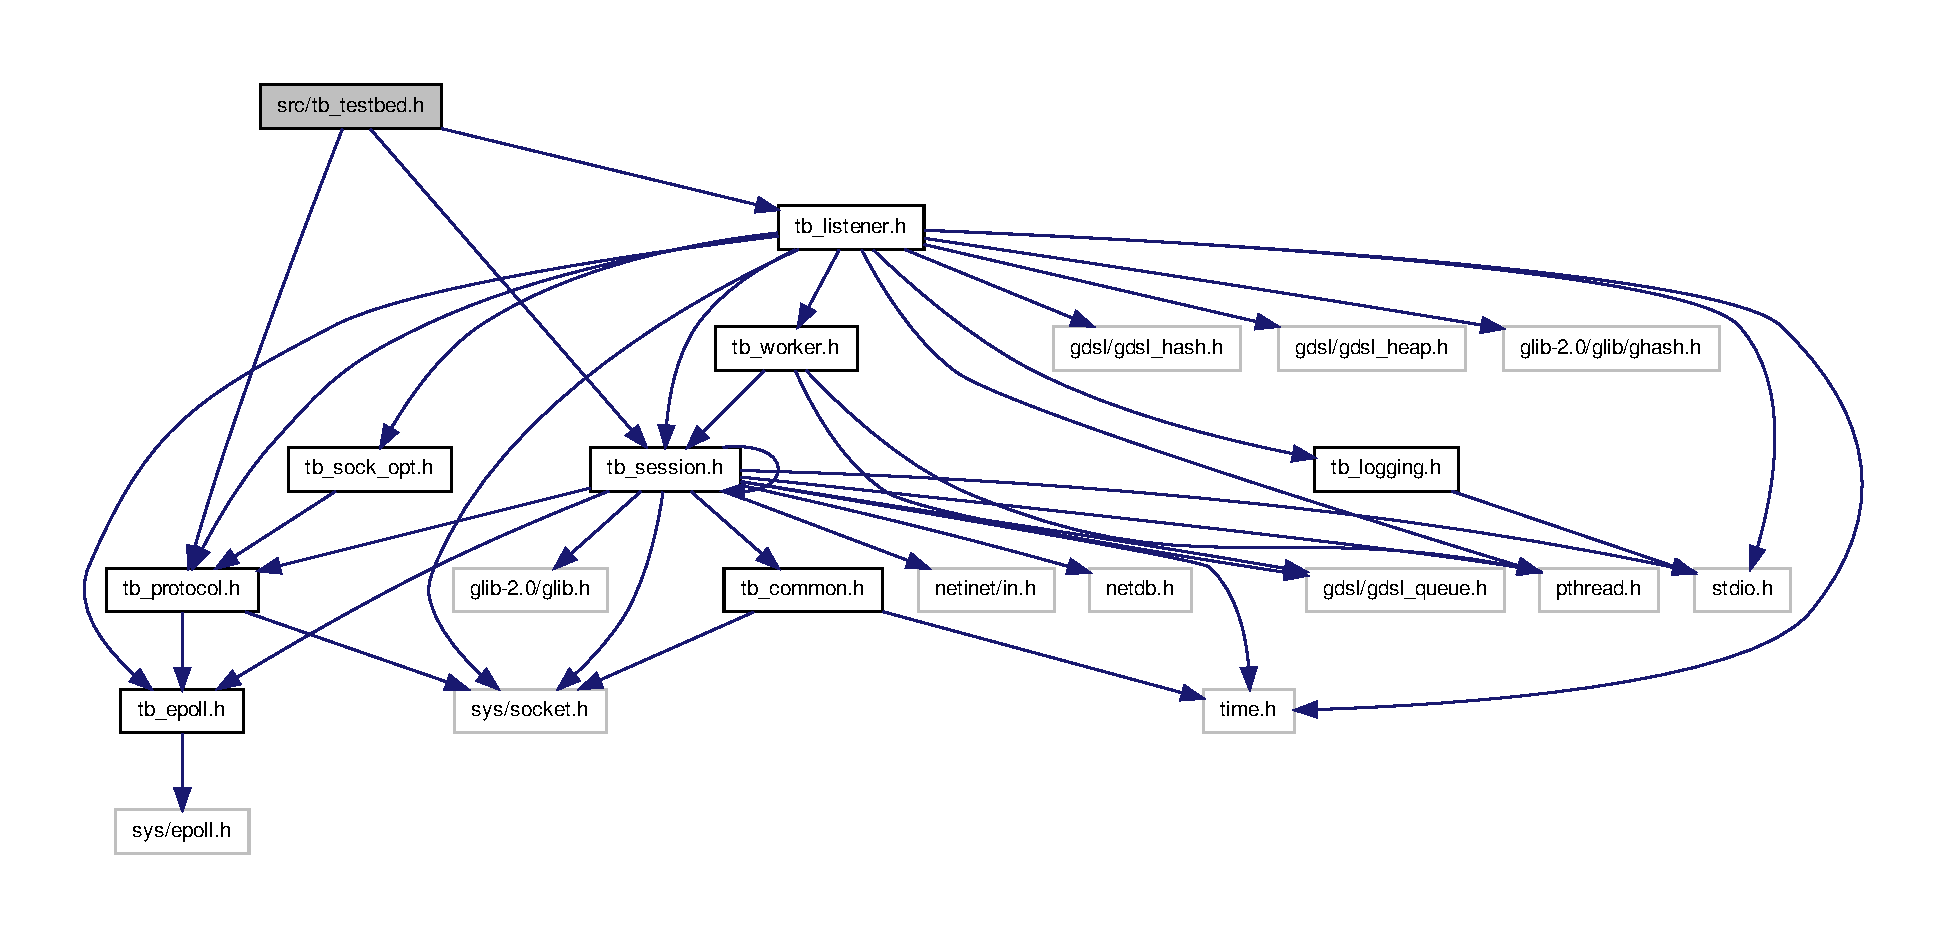
\includegraphics[width=350pt]{tb__testbed_8h__incl}
\end{center}
\end{figure}
This graph shows which files directly or indirectly include this file\-:\nopagebreak
\begin{figure}[H]
\begin{center}
\leavevmode
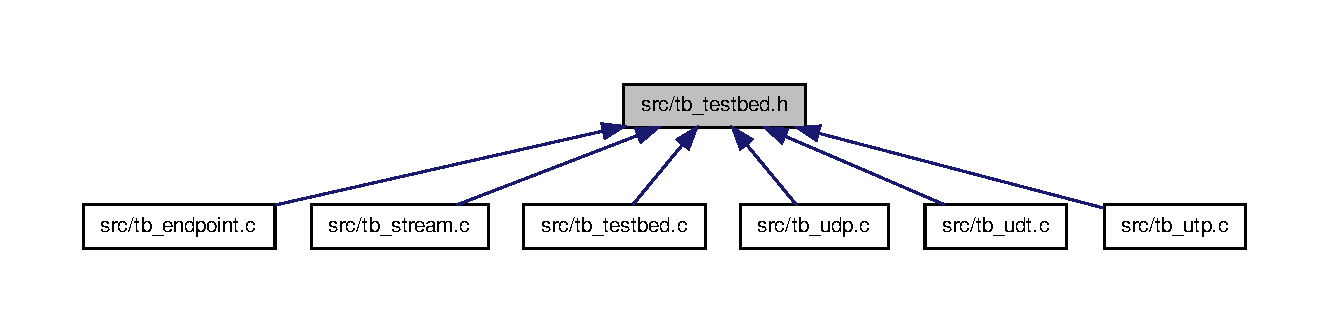
\includegraphics[width=350pt]{tb__testbed_8h__dep__incl}
\end{center}
\end{figure}
\subsection*{Enumerations}
\begin{DoxyCompactItemize}
\item 
enum \hyperlink{tb__testbed_8h_ab81ca9153c95d55639b4ab520bb2aa4d}{I\-N\-P\-U\-T} \{ \\*
\hyperlink{tb__testbed_8h_ab81ca9153c95d55639b4ab520bb2aa4dab47ea8bb955afd0adc0ef98517dd6084}{T\-Y\-P\-E} =  1, 
\hyperlink{tb__testbed_8h_ab81ca9153c95d55639b4ab520bb2aa4da4fabbaac7b5e57d7b8b019a0f79ce492}{A\-D\-D\-R\-E\-S\-S}, 
\hyperlink{tb__testbed_8h_ab81ca9153c95d55639b4ab520bb2aa4da8268527d969e4ef493d3f35844a0b841}{P\-O\-R\-T}, 
\hyperlink{tb__testbed_8h_ab81ca9153c95d55639b4ab520bb2aa4da4965c5a2738945d912c8afcbfe435ad1}{P\-R\-O\-T}, 
\\*
\hyperlink{tb__testbed_8h_ab81ca9153c95d55639b4ab520bb2aa4da98bdbe98880b7a360d1ecc8a19f5677d}{B\-U\-F\-\_\-\-S\-I\-Z\-E}, 
\hyperlink{tb__testbed_8h_ab81ca9153c95d55639b4ab520bb2aa4da1d55968a1d035b4ae659e3234264a899}{F\-I\-L\-E\-\_\-\-T\-Y\-P\-E}, 
\hyperlink{tb__testbed_8h_ab81ca9153c95d55639b4ab520bb2aa4da77374a65274f20cc342c53cc2fd52ea0}{F\-I\-L\-E\-\_\-\-N\-A\-M\-E}
 \}
\end{DoxyCompactItemize}
\subsection*{Functions}
\begin{DoxyCompactItemize}
\item 
\hyperlink{structtb__listener__t}{tb\-\_\-listener\-\_\-t} $\ast$ \hyperlink{tb__testbed_8h_a5ec3b6c120621050965582e51e4d0d5a}{tb\-\_\-create\-\_\-listener} (\hyperlink{tb__listener_8h_ae37f3ebcf0081b2dd11adf41f1f867d6}{E\-N\-D\-P\-O\-I\-N\-T\-\_\-\-T\-Y\-P\-E} type, char $\ast$addr, char $\ast$port, \hyperlink{tb__protocol_8h_a7a5bff1040fc154c510874327d44cc1a}{P\-R\-O\-T\-O\-C\-O\-L} protocol, int bufsize)
\begin{DoxyCompactList}\small\item\em Create a listener with the supplied parameters. \end{DoxyCompactList}\item 
\hyperlink{structtb__listener__t}{tb\-\_\-listener\-\_\-t} $\ast$ \hyperlink{tb__testbed_8h_a042a2b565ccc70e1506562ad43c83bfb}{tb\-\_\-create\-\_\-endpoint} (\hyperlink{structtb__test__params__t}{tb\-\_\-test\-\_\-params\-\_\-t} $\ast$params)
\begin{DoxyCompactList}\small\item\em Create a listener using a \hyperlink{structtb__test__params__t}{tb\-\_\-test\-\_\-params\-\_\-t} struct. \end{DoxyCompactList}\item 
\hyperlink{structtb__prot__stats__t}{tb\-\_\-prot\-\_\-stats\-\_\-t} $\ast$ \hyperlink{tb__testbed_8h_a7e28b461066b5dd420523dc686b3ac29}{tb\-\_\-get\-\_\-protocol\-\_\-stats} (\hyperlink{structtb__listener__t}{tb\-\_\-listener\-\_\-t} $\ast$listener)
\item 
\hyperlink{structtb__prot__stats__t}{tb\-\_\-prot\-\_\-stats\-\_\-t} $\ast$ \hyperlink{tb__testbed_8h_a6e5c88a915882ea9d39fd41ee4742ffc}{tb\-\_\-ex\-\_\-get\-\_\-stats} (\hyperlink{structtb__listener__t}{tb\-\_\-listener\-\_\-t} $\ast$listener)
\begin{DoxyCompactList}\small\item\em A thread safe way to get access to stats. \end{DoxyCompactList}\item 
int \hyperlink{tb__testbed_8h_a3be49a9767c918bd4abcb1e6ba44f014}{tb\-\_\-parse} (int argc, char $\ast$argv\mbox{[}$\,$\mbox{]})
\begin{DoxyCompactList}\small\item\em Parse input from a number of strings. \end{DoxyCompactList}\item 
int \hyperlink{tb__testbed_8h_ac8da963855e09bf929c085486f4a3b47}{test} ()
\item 
void \hyperlink{tb__testbed_8h_a70047050ccc93bb63209038b7d6d9284}{tb\-\_\-start} (\hyperlink{structtb__listener__t}{tb\-\_\-listener\-\_\-t} $\ast$listener)
\begin{DoxyCompactList}\small\item\em Starts the server/client. \end{DoxyCompactList}\item 
int \hyperlink{tb__testbed_8h_ab77c10c1456bceb81a136fbf41a68cb8}{tb\-\_\-monitor} (\hyperlink{structtb__listener__t}{tb\-\_\-listener\-\_\-t} $\ast$listener)
\begin{DoxyCompactList}\small\item\em actively monitor the server/client connection \end{DoxyCompactList}\item 
void \hyperlink{tb__testbed_8h_af588c4b48b411318fac6057a5399512d}{tb\-\_\-print\-\_\-stats} (\hyperlink{structtb__prot__stats__t}{tb\-\_\-prot\-\_\-stats\-\_\-t} $\ast$stats, \hyperlink{structtb__listener__t}{tb\-\_\-listener\-\_\-t} $\ast$listener)
\begin{DoxyCompactList}\small\item\em Print the stats given. \end{DoxyCompactList}\item 
void \hyperlink{tb__testbed_8h_a31e07ac64cefdac833246c5c845449b7}{tb\-\_\-interrupt\-\_\-handler} (int value)
\begin{DoxyCompactList}\small\item\em Handle system interrupts. \end{DoxyCompactList}\item 
void \hyperlink{tb__testbed_8h_ad77d79cfa8de8247ef4166ea49aec63f}{tb\-\_\-abort} (void $\ast$data) \-\_\-\-\_\-attribute\-\_\-\-\_\-((\-\_\-\-\_\-noreturn\-\_\-\-\_\-))
\begin{DoxyCompactList}\small\item\em Aborts program. \end{DoxyCompactList}\item 
void \hyperlink{tb__testbed_8h_a75ea5c908edfd87375f5bc7b8653232e}{tb\-\_\-exit} (void $\ast$data) \-\_\-\-\_\-attribute\-\_\-\-\_\-((\-\_\-\-\_\-noreturn\-\_\-\-\_\-))
\begin{DoxyCompactList}\small\item\em Exits program. \end{DoxyCompactList}\end{DoxyCompactItemize}
\subsection*{Variables}
\begin{DoxyCompactItemize}
\item 
const int \hyperlink{tb__testbed_8h_a16bd599f12a21e98f33152764b85ae37}{C\-\_\-\-B\-U\-F\-F\-\_\-\-S\-I\-Z\-E}
\begin{DoxyCompactList}\small\item\em The client buffer multiplier. \end{DoxyCompactList}\item 
const int \hyperlink{tb__testbed_8h_ab5ee406d514403c7caaa5bce873cd300}{S\-\_\-\-B\-U\-F\-F\-\_\-\-S\-I\-Z\-E}
\begin{DoxyCompactList}\small\item\em The server buffer multiplier. \end{DoxyCompactList}\end{DoxyCompactItemize}


\subsection{Enumeration Type Documentation}
\hypertarget{tb__testbed_8h_ab81ca9153c95d55639b4ab520bb2aa4d}{\index{tb\-\_\-testbed.\-h@{tb\-\_\-testbed.\-h}!I\-N\-P\-U\-T@{I\-N\-P\-U\-T}}
\index{I\-N\-P\-U\-T@{I\-N\-P\-U\-T}!tb_testbed.h@{tb\-\_\-testbed.\-h}}
\subsubsection[{I\-N\-P\-U\-T}]{\setlength{\rightskip}{0pt plus 5cm}enum {\bf I\-N\-P\-U\-T}}}\label{tb__testbed_8h_ab81ca9153c95d55639b4ab520bb2aa4d}
\begin{Desc}
\item[Enumerator\-: ]\par
\begin{description}
\index{T\-Y\-P\-E@{T\-Y\-P\-E}!tb\-\_\-testbed.\-h@{tb\-\_\-testbed.\-h}}\index{tb\-\_\-testbed.\-h@{tb\-\_\-testbed.\-h}!T\-Y\-P\-E@{T\-Y\-P\-E}}\item[{\em 
\hypertarget{tb__testbed_8h_ab81ca9153c95d55639b4ab520bb2aa4dab47ea8bb955afd0adc0ef98517dd6084}{T\-Y\-P\-E}\label{tb__testbed_8h_ab81ca9153c95d55639b4ab520bb2aa4dab47ea8bb955afd0adc0ef98517dd6084}
}]The type of endpoint to create (server, client) \index{A\-D\-D\-R\-E\-S\-S@{A\-D\-D\-R\-E\-S\-S}!tb\-\_\-testbed.\-h@{tb\-\_\-testbed.\-h}}\index{tb\-\_\-testbed.\-h@{tb\-\_\-testbed.\-h}!A\-D\-D\-R\-E\-S\-S@{A\-D\-D\-R\-E\-S\-S}}\item[{\em 
\hypertarget{tb__testbed_8h_ab81ca9153c95d55639b4ab520bb2aa4da4fabbaac7b5e57d7b8b019a0f79ce492}{A\-D\-D\-R\-E\-S\-S}\label{tb__testbed_8h_ab81ca9153c95d55639b4ab520bb2aa4da4fabbaac7b5e57d7b8b019a0f79ce492}
}]The address to bind/connect to. \index{P\-O\-R\-T@{P\-O\-R\-T}!tb\-\_\-testbed.\-h@{tb\-\_\-testbed.\-h}}\index{tb\-\_\-testbed.\-h@{tb\-\_\-testbed.\-h}!P\-O\-R\-T@{P\-O\-R\-T}}\item[{\em 
\hypertarget{tb__testbed_8h_ab81ca9153c95d55639b4ab520bb2aa4da8268527d969e4ef493d3f35844a0b841}{P\-O\-R\-T}\label{tb__testbed_8h_ab81ca9153c95d55639b4ab520bb2aa4da8268527d969e4ef493d3f35844a0b841}
}]The port to bind/connect to. \index{P\-R\-O\-T@{P\-R\-O\-T}!tb\-\_\-testbed.\-h@{tb\-\_\-testbed.\-h}}\index{tb\-\_\-testbed.\-h@{tb\-\_\-testbed.\-h}!P\-R\-O\-T@{P\-R\-O\-T}}\item[{\em 
\hypertarget{tb__testbed_8h_ab81ca9153c95d55639b4ab520bb2aa4da4965c5a2738945d912c8afcbfe435ad1}{P\-R\-O\-T}\label{tb__testbed_8h_ab81ca9153c95d55639b4ab520bb2aa4da4965c5a2738945d912c8afcbfe435ad1}
}]The protocol to use. \index{B\-U\-F\-\_\-\-S\-I\-Z\-E@{B\-U\-F\-\_\-\-S\-I\-Z\-E}!tb\-\_\-testbed.\-h@{tb\-\_\-testbed.\-h}}\index{tb\-\_\-testbed.\-h@{tb\-\_\-testbed.\-h}!B\-U\-F\-\_\-\-S\-I\-Z\-E@{B\-U\-F\-\_\-\-S\-I\-Z\-E}}\item[{\em 
\hypertarget{tb__testbed_8h_ab81ca9153c95d55639b4ab520bb2aa4da98bdbe98880b7a360d1ecc8a19f5677d}{B\-U\-F\-\_\-\-S\-I\-Z\-E}\label{tb__testbed_8h_ab81ca9153c95d55639b4ab520bb2aa4da98bdbe98880b7a360d1ecc8a19f5677d}
}]The size of the application buffer to use. \index{F\-I\-L\-E\-\_\-\-T\-Y\-P\-E@{F\-I\-L\-E\-\_\-\-T\-Y\-P\-E}!tb\-\_\-testbed.\-h@{tb\-\_\-testbed.\-h}}\index{tb\-\_\-testbed.\-h@{tb\-\_\-testbed.\-h}!F\-I\-L\-E\-\_\-\-T\-Y\-P\-E@{F\-I\-L\-E\-\_\-\-T\-Y\-P\-E}}\item[{\em 
\hypertarget{tb__testbed_8h_ab81ca9153c95d55639b4ab520bb2aa4da1d55968a1d035b4ae659e3234264a899}{F\-I\-L\-E\-\_\-\-T\-Y\-P\-E}\label{tb__testbed_8h_ab81ca9153c95d55639b4ab520bb2aa4da1d55968a1d035b4ae659e3234264a899}
}]The type of file to use (disk file, random R\-A\-M file) \index{F\-I\-L\-E\-\_\-\-N\-A\-M\-E@{F\-I\-L\-E\-\_\-\-N\-A\-M\-E}!tb\-\_\-testbed.\-h@{tb\-\_\-testbed.\-h}}\index{tb\-\_\-testbed.\-h@{tb\-\_\-testbed.\-h}!F\-I\-L\-E\-\_\-\-N\-A\-M\-E@{F\-I\-L\-E\-\_\-\-N\-A\-M\-E}}\item[{\em 
\hypertarget{tb__testbed_8h_ab81ca9153c95d55639b4ab520bb2aa4da77374a65274f20cc342c53cc2fd52ea0}{F\-I\-L\-E\-\_\-\-N\-A\-M\-E}\label{tb__testbed_8h_ab81ca9153c95d55639b4ab520bb2aa4da77374a65274f20cc342c53cc2fd52ea0}
}]The name of the file or the size of the random file To use. \end{description}
\end{Desc}



Definition at line 18 of file tb\-\_\-testbed.\-h.



\subsection{Function Documentation}
\hypertarget{tb__testbed_8h_ad77d79cfa8de8247ef4166ea49aec63f}{\index{tb\-\_\-testbed.\-h@{tb\-\_\-testbed.\-h}!tb\-\_\-abort@{tb\-\_\-abort}}
\index{tb\-\_\-abort@{tb\-\_\-abort}!tb_testbed.h@{tb\-\_\-testbed.\-h}}
\subsubsection[{tb\-\_\-abort}]{\setlength{\rightskip}{0pt plus 5cm}void tb\-\_\-abort (
\begin{DoxyParamCaption}
\item[{void $\ast$}]{data}
\end{DoxyParamCaption}
)}}\label{tb__testbed_8h_ad77d79cfa8de8247ef4166ea49aec63f}


Aborts program. 

Aborts the program, closes the listener and underlying protocol, kills any sockets or files still open.


\begin{DoxyParams}{Parameters}
{\em listener} & The listener to close/destroy. \\
\hline
\end{DoxyParams}


Definition at line 445 of file tb\-\_\-testbed.\-c.

\hypertarget{tb__testbed_8h_a042a2b565ccc70e1506562ad43c83bfb}{\index{tb\-\_\-testbed.\-h@{tb\-\_\-testbed.\-h}!tb\-\_\-create\-\_\-endpoint@{tb\-\_\-create\-\_\-endpoint}}
\index{tb\-\_\-create\-\_\-endpoint@{tb\-\_\-create\-\_\-endpoint}!tb_testbed.h@{tb\-\_\-testbed.\-h}}
\subsubsection[{tb\-\_\-create\-\_\-endpoint}]{\setlength{\rightskip}{0pt plus 5cm}{\bf tb\-\_\-listener\-\_\-t}$\ast$ tb\-\_\-create\-\_\-endpoint (
\begin{DoxyParamCaption}
\item[{{\bf tb\-\_\-test\-\_\-params\-\_\-t} $\ast$}]{params}
\end{DoxyParamCaption}
)}}\label{tb__testbed_8h_a042a2b565ccc70e1506562ad43c83bfb}


Create a listener using a \hyperlink{structtb__test__params__t}{tb\-\_\-test\-\_\-params\-\_\-t} struct. 

The details in the struct are used to create an endpoint for use in testing.


\begin{DoxyParams}{Parameters}
{\em params} & A struct with all of the required details for a test. \\
\hline
\end{DoxyParams}
\begin{DoxyReturn}{Returns}
the endpoint to test with. 
\end{DoxyReturn}


Definition at line 158 of file tb\-\_\-listener.\-c.

\hypertarget{tb__testbed_8h_a5ec3b6c120621050965582e51e4d0d5a}{\index{tb\-\_\-testbed.\-h@{tb\-\_\-testbed.\-h}!tb\-\_\-create\-\_\-listener@{tb\-\_\-create\-\_\-listener}}
\index{tb\-\_\-create\-\_\-listener@{tb\-\_\-create\-\_\-listener}!tb_testbed.h@{tb\-\_\-testbed.\-h}}
\subsubsection[{tb\-\_\-create\-\_\-listener}]{\setlength{\rightskip}{0pt plus 5cm}{\bf tb\-\_\-listener\-\_\-t}$\ast$ tb\-\_\-create\-\_\-listener (
\begin{DoxyParamCaption}
\item[{{\bf E\-N\-D\-P\-O\-I\-N\-T\-\_\-\-T\-Y\-P\-E}}]{type, }
\item[{char $\ast$}]{addr, }
\item[{char $\ast$}]{port, }
\item[{{\bf P\-R\-O\-T\-O\-C\-O\-L}}]{protocol, }
\item[{int}]{bufsize}
\end{DoxyParamCaption}
)}}\label{tb__testbed_8h_a5ec3b6c120621050965582e51e4d0d5a}


Create a listener with the supplied parameters. 

Creates a listener and the accociated data structures.


\begin{DoxyParams}{Parameters}
{\em type} & The type of endpoint to create. \\
\hline
{\em addr} & The address to bind to. \\
\hline
{\em port} & The port to bind to. \\
\hline
{\em num\-\_\-threads} & The number of worker threads to use.\\
\hline
\end{DoxyParams}
\begin{DoxyReturn}{Returns}
The newly created listener. 
\end{DoxyReturn}


Definition at line 38 of file tb\-\_\-listener.\-c.

\hypertarget{tb__testbed_8h_a6e5c88a915882ea9d39fd41ee4742ffc}{\index{tb\-\_\-testbed.\-h@{tb\-\_\-testbed.\-h}!tb\-\_\-ex\-\_\-get\-\_\-stats@{tb\-\_\-ex\-\_\-get\-\_\-stats}}
\index{tb\-\_\-ex\-\_\-get\-\_\-stats@{tb\-\_\-ex\-\_\-get\-\_\-stats}!tb_testbed.h@{tb\-\_\-testbed.\-h}}
\subsubsection[{tb\-\_\-ex\-\_\-get\-\_\-stats}]{\setlength{\rightskip}{0pt plus 5cm}{\bf tb\-\_\-prot\-\_\-stats\-\_\-t}$\ast$ tb\-\_\-ex\-\_\-get\-\_\-stats (
\begin{DoxyParamCaption}
\item[{{\bf tb\-\_\-listener\-\_\-t} $\ast$}]{listener}
\end{DoxyParamCaption}
)}}\label{tb__testbed_8h_a6e5c88a915882ea9d39fd41ee4742ffc}


A thread safe way to get access to stats. 

This method controls access to the stats generated by testbed. These stats are updated every second, and can be read once. If the data that can be obtained by this function has already been read, it blocks until new data has arrived.


\begin{DoxyParams}{Parameters}
{\em listener} & The listener for which to get the stats from. \\
\hline
\end{DoxyParams}
\begin{DoxyReturn}{Returns}
\hyperlink{structtb__prot__stats__t}{tb\-\_\-prot\-\_\-stats\-\_\-t} with the stats inserted. 
\end{DoxyReturn}


Definition at line 362 of file tb\-\_\-listener.\-c.

\hypertarget{tb__testbed_8h_a75ea5c908edfd87375f5bc7b8653232e}{\index{tb\-\_\-testbed.\-h@{tb\-\_\-testbed.\-h}!tb\-\_\-exit@{tb\-\_\-exit}}
\index{tb\-\_\-exit@{tb\-\_\-exit}!tb_testbed.h@{tb\-\_\-testbed.\-h}}
\subsubsection[{tb\-\_\-exit}]{\setlength{\rightskip}{0pt plus 5cm}void tb\-\_\-exit (
\begin{DoxyParamCaption}
\item[{void $\ast$}]{data}
\end{DoxyParamCaption}
)}}\label{tb__testbed_8h_a75ea5c908edfd87375f5bc7b8653232e}


Exits program. 

Exits the program, closes the listener and underlying protocol, kills any sockes or files still open.


\begin{DoxyParams}{Parameters}
{\em listener} & The listener to close/destroy. \\
\hline
\end{DoxyParams}


Definition at line 434 of file tb\-\_\-testbed.\-c.

\hypertarget{tb__testbed_8h_a7e28b461066b5dd420523dc686b3ac29}{\index{tb\-\_\-testbed.\-h@{tb\-\_\-testbed.\-h}!tb\-\_\-get\-\_\-protocol\-\_\-stats@{tb\-\_\-get\-\_\-protocol\-\_\-stats}}
\index{tb\-\_\-get\-\_\-protocol\-\_\-stats@{tb\-\_\-get\-\_\-protocol\-\_\-stats}!tb_testbed.h@{tb\-\_\-testbed.\-h}}
\subsubsection[{tb\-\_\-get\-\_\-protocol\-\_\-stats}]{\setlength{\rightskip}{0pt plus 5cm}{\bf tb\-\_\-prot\-\_\-stats\-\_\-t}$\ast$ tb\-\_\-get\-\_\-protocol\-\_\-stats (
\begin{DoxyParamCaption}
\item[{{\bf tb\-\_\-listener\-\_\-t} $\ast$}]{listener}
\end{DoxyParamCaption}
)}}\label{tb__testbed_8h_a7e28b461066b5dd420523dc686b3ac29}
\hypertarget{tb__testbed_8h_a31e07ac64cefdac833246c5c845449b7}{\index{tb\-\_\-testbed.\-h@{tb\-\_\-testbed.\-h}!tb\-\_\-interrupt\-\_\-handler@{tb\-\_\-interrupt\-\_\-handler}}
\index{tb\-\_\-interrupt\-\_\-handler@{tb\-\_\-interrupt\-\_\-handler}!tb_testbed.h@{tb\-\_\-testbed.\-h}}
\subsubsection[{tb\-\_\-interrupt\-\_\-handler}]{\setlength{\rightskip}{0pt plus 5cm}void tb\-\_\-interrupt\-\_\-handler (
\begin{DoxyParamCaption}
\item[{int}]{value}
\end{DoxyParamCaption}
)}}\label{tb__testbed_8h_a31e07ac64cefdac833246c5c845449b7}


Handle system interrupts. 

Handles system interrupts, and kills the client/server if one is received.


\begin{DoxyParams}{Parameters}
{\em value} & Value passed by the signal. \\
\hline
\end{DoxyParams}
\hypertarget{tb__testbed_8h_ab77c10c1456bceb81a136fbf41a68cb8}{\index{tb\-\_\-testbed.\-h@{tb\-\_\-testbed.\-h}!tb\-\_\-monitor@{tb\-\_\-monitor}}
\index{tb\-\_\-monitor@{tb\-\_\-monitor}!tb_testbed.h@{tb\-\_\-testbed.\-h}}
\subsubsection[{tb\-\_\-monitor}]{\setlength{\rightskip}{0pt plus 5cm}int tb\-\_\-monitor (
\begin{DoxyParamCaption}
\item[{{\bf tb\-\_\-listener\-\_\-t} $\ast$}]{listener}
\end{DoxyParamCaption}
)}}\label{tb__testbed_8h_ab77c10c1456bceb81a136fbf41a68cb8}


actively monitor the server/client connection 


\begin{DoxyParams}{Parameters}
{\em listener} & The listener to monitor. \\
\hline
\end{DoxyParams}


Definition at line 300 of file tb\-\_\-testbed.\-c.

\hypertarget{tb__testbed_8h_a3be49a9767c918bd4abcb1e6ba44f014}{\index{tb\-\_\-testbed.\-h@{tb\-\_\-testbed.\-h}!tb\-\_\-parse@{tb\-\_\-parse}}
\index{tb\-\_\-parse@{tb\-\_\-parse}!tb_testbed.h@{tb\-\_\-testbed.\-h}}
\subsubsection[{tb\-\_\-parse}]{\setlength{\rightskip}{0pt plus 5cm}int tb\-\_\-parse (
\begin{DoxyParamCaption}
\item[{int}]{argc, }
\item[{char $\ast$}]{argv\mbox{[}$\,$\mbox{]}}
\end{DoxyParamCaption}
)}}\label{tb__testbed_8h_a3be49a9767c918bd4abcb1e6ba44f014}


Parse input from a number of strings. 

Parses values from strings, to create a server or client


\begin{DoxyParams}{Parameters}
{\em argc} & The number of input strings. \\
\hline
{\em argv} & The strings. \\
\hline
\end{DoxyParams}
\begin{DoxyReturn}{Returns}
0 if the setup was successful.
\end{DoxyReturn}
argv\mbox{[}0\mbox{]} = Test\-Bed argv\mbox{[}1\mbox{]} = Type (server, client) argv\mbox{[}2\mbox{]} = Address argv\mbox{[}3\mbox{]} = Port argv\mbox{[}4\mbox{]} = Protocol (tcp, udp, udt) argv\mbox{[}5\mbox{]} = Bufsize (M\-B) argv\mbox{[}6\mbox{]} = File type (size, file) argv\mbox{[}7\mbox{]} = Filename/\-Fliesize 

Definition at line 63 of file tb\-\_\-testbed.\-c.

\hypertarget{tb__testbed_8h_af588c4b48b411318fac6057a5399512d}{\index{tb\-\_\-testbed.\-h@{tb\-\_\-testbed.\-h}!tb\-\_\-print\-\_\-stats@{tb\-\_\-print\-\_\-stats}}
\index{tb\-\_\-print\-\_\-stats@{tb\-\_\-print\-\_\-stats}!tb_testbed.h@{tb\-\_\-testbed.\-h}}
\subsubsection[{tb\-\_\-print\-\_\-stats}]{\setlength{\rightskip}{0pt plus 5cm}void tb\-\_\-print\-\_\-stats (
\begin{DoxyParamCaption}
\item[{{\bf tb\-\_\-prot\-\_\-stats\-\_\-t} $\ast$}]{stats, }
\item[{{\bf tb\-\_\-listener\-\_\-t} $\ast$}]{listener}
\end{DoxyParamCaption}
)}}\label{tb__testbed_8h_af588c4b48b411318fac6057a5399512d}


Print the stats given. 


\begin{DoxyParams}{Parameters}
{\em stats} & The stats struct to print. \\
\hline
{\em listener} & The listener to print stats for. \\
\hline
\end{DoxyParams}


Definition at line 401 of file tb\-\_\-testbed.\-c.

\hypertarget{tb__testbed_8h_a70047050ccc93bb63209038b7d6d9284}{\index{tb\-\_\-testbed.\-h@{tb\-\_\-testbed.\-h}!tb\-\_\-start@{tb\-\_\-start}}
\index{tb\-\_\-start@{tb\-\_\-start}!tb_testbed.h@{tb\-\_\-testbed.\-h}}
\subsubsection[{tb\-\_\-start}]{\setlength{\rightskip}{0pt plus 5cm}void tb\-\_\-start (
\begin{DoxyParamCaption}
\item[{{\bf tb\-\_\-listener\-\_\-t} $\ast$}]{listener}
\end{DoxyParamCaption}
)}}\label{tb__testbed_8h_a70047050ccc93bb63209038b7d6d9284}


Starts the server/client. 

This begins the server or client. Filename can be null if the endpoint is a server.


\begin{DoxyParams}{Parameters}
{\em listener} & The listener to start. \\
\hline
\end{DoxyParams}
\begin{DoxyReturn}{Returns}
0 if performed. 
\end{DoxyReturn}


Definition at line 211 of file tb\-\_\-testbed.\-c.

\hypertarget{tb__testbed_8h_ac8da963855e09bf929c085486f4a3b47}{\index{tb\-\_\-testbed.\-h@{tb\-\_\-testbed.\-h}!test@{test}}
\index{test@{test}!tb_testbed.h@{tb\-\_\-testbed.\-h}}
\subsubsection[{test}]{\setlength{\rightskip}{0pt plus 5cm}int test (
\begin{DoxyParamCaption}
{}
\end{DoxyParamCaption}
)}}\label{tb__testbed_8h_ac8da963855e09bf929c085486f4a3b47}


Definition at line 45 of file tb\-\_\-testbed.\-c.



\subsection{Variable Documentation}
\hypertarget{tb__testbed_8h_a16bd599f12a21e98f33152764b85ae37}{\index{tb\-\_\-testbed.\-h@{tb\-\_\-testbed.\-h}!C\-\_\-\-B\-U\-F\-F\-\_\-\-S\-I\-Z\-E@{C\-\_\-\-B\-U\-F\-F\-\_\-\-S\-I\-Z\-E}}
\index{C\-\_\-\-B\-U\-F\-F\-\_\-\-S\-I\-Z\-E@{C\-\_\-\-B\-U\-F\-F\-\_\-\-S\-I\-Z\-E}!tb_testbed.h@{tb\-\_\-testbed.\-h}}
\subsubsection[{C\-\_\-\-B\-U\-F\-F\-\_\-\-S\-I\-Z\-E}]{\setlength{\rightskip}{0pt plus 5cm}const int C\-\_\-\-B\-U\-F\-F\-\_\-\-S\-I\-Z\-E}}\label{tb__testbed_8h_a16bd599f12a21e98f33152764b85ae37}


The client buffer multiplier. 

The size provided by the user at run time is multiplied by this number to generate the buffer size. \hypertarget{tb__testbed_8h_ab5ee406d514403c7caaa5bce873cd300}{\index{tb\-\_\-testbed.\-h@{tb\-\_\-testbed.\-h}!S\-\_\-\-B\-U\-F\-F\-\_\-\-S\-I\-Z\-E@{S\-\_\-\-B\-U\-F\-F\-\_\-\-S\-I\-Z\-E}}
\index{S\-\_\-\-B\-U\-F\-F\-\_\-\-S\-I\-Z\-E@{S\-\_\-\-B\-U\-F\-F\-\_\-\-S\-I\-Z\-E}!tb_testbed.h@{tb\-\_\-testbed.\-h}}
\subsubsection[{S\-\_\-\-B\-U\-F\-F\-\_\-\-S\-I\-Z\-E}]{\setlength{\rightskip}{0pt plus 5cm}const int S\-\_\-\-B\-U\-F\-F\-\_\-\-S\-I\-Z\-E}}\label{tb__testbed_8h_ab5ee406d514403c7caaa5bce873cd300}


The server buffer multiplier. 

The size provided by the user at run time is multiplited by this number to generate the buffer size. 
\hypertarget{tb__udp_8c}{\section{src/tb\-\_\-udp.c File Reference}
\label{tb__udp_8c}\index{src/tb\-\_\-udp.\-c@{src/tb\-\_\-udp.\-c}}
}
{\ttfamily \#include \char`\"{}tb\-\_\-udp.\-h\char`\"{}}\\*
{\ttfamily \#include \char`\"{}tb\-\_\-epoll.\-h\char`\"{}}\\*
{\ttfamily \#include \char`\"{}tb\-\_\-session.\-h\char`\"{}}\\*
{\ttfamily \#include \char`\"{}tb\-\_\-common.\-h\char`\"{}}\\*
{\ttfamily \#include \char`\"{}tb\-\_\-listener.\-h\char`\"{}}\\*
{\ttfamily \#include \char`\"{}tb\-\_\-worker.\-h\char`\"{}}\\*
{\ttfamily \#include \char`\"{}tb\-\_\-utp.\-h\char`\"{}}\\*
{\ttfamily \#include \char`\"{}tb\-\_\-testbed.\-h\char`\"{}}\\*
{\ttfamily \#include $<$stdio.\-h$>$}\\*
{\ttfamily \#include $<$stdlib.\-h$>$}\\*
{\ttfamily \#include $<$assert.\-h$>$}\\*
{\ttfamily \#include $<$pthread.\-h$>$}\\*
{\ttfamily \#include $<$sys/socket.\-h$>$}\\*
{\ttfamily \#include $<$fcntl.\-h$>$}\\*
{\ttfamily \#include $<$unistd.\-h$>$}\\*
{\ttfamily \#include $<$string.\-h$>$}\\*
{\ttfamily \#include $<$sys/epoll.\-h$>$}\\*
{\ttfamily \#include $<$time.\-h$>$}\\*
{\ttfamily \#include $<$sys/ioctl.\-h$>$}\\*
{\ttfamily \#include $<$netinet/in.\-h$>$}\\*
{\ttfamily \#include $<$netdb.\-h$>$}\\*
{\ttfamily \#include $<$udt.\-h$>$}\\*
{\ttfamily \#include $<$errno.\-h$>$}\\*
Include dependency graph for tb\-\_\-udp.\-c\-:\nopagebreak
\begin{figure}[H]
\begin{center}
\leavevmode
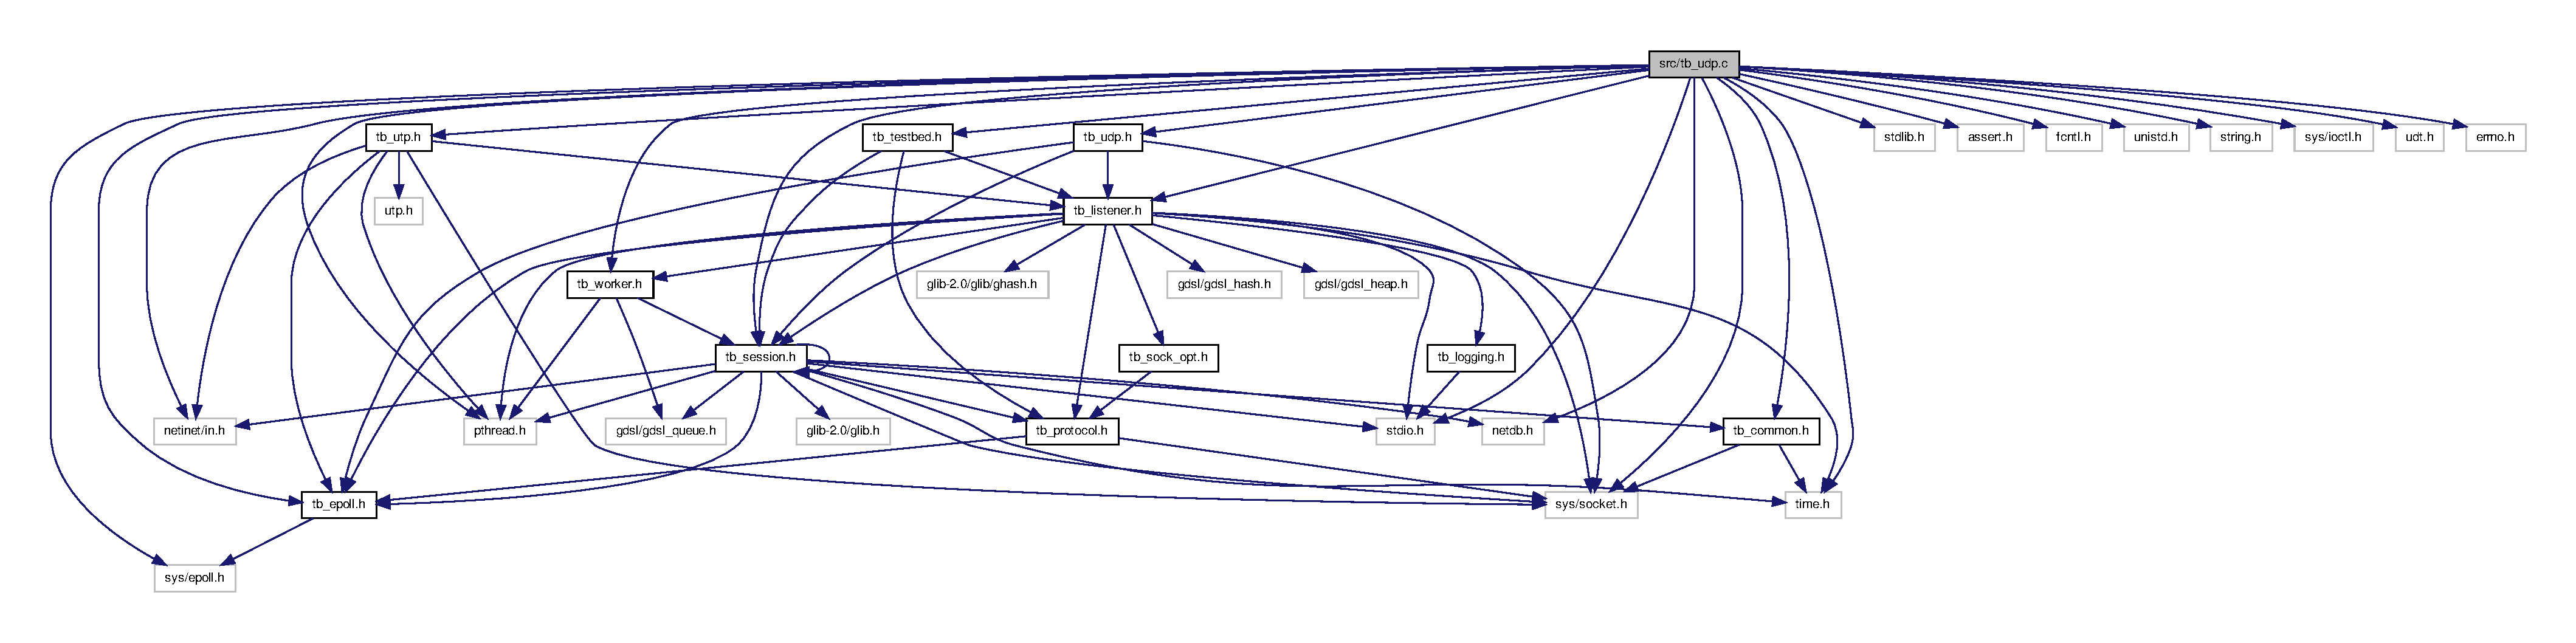
\includegraphics[width=350pt]{tb__udp_8c__incl}
\end{center}
\end{figure}
\subsection*{Functions}
\begin{DoxyCompactItemize}
\item 
int \hyperlink{tb__udp_8c_a2d630c38c6c37789b56d70a575a1eeb5}{tb\-\_\-udp\-\_\-client} (\hyperlink{structtb__listener__t}{tb\-\_\-listener\-\_\-t} $\ast$listener)
\begin{DoxyCompactList}\small\item\em Upload a file using udp with epoll eof ack. \end{DoxyCompactList}\item 
int \hyperlink{tb__udp_8c_ac1be4ad75f9aa84b62a3cd530f822ea9}{tb\-\_\-udp\-\_\-ack} (int events, void $\ast$data)
\begin{DoxyCompactList}\small\item\em Callback function for udp. \end{DoxyCompactList}\item 
int \hyperlink{tb__udp_8c_a0e726d76f273fe0f7d77d569bbe481c0}{tb\-\_\-udp\-\_\-epoll\-\_\-client} (\hyperlink{structtb__listener__t}{tb\-\_\-listener\-\_\-t} $\ast$listener)
\begin{DoxyCompactList}\small\item\em Uses epoll for receiving data from the client. This is a prototype for T\-B0.\-2. \end{DoxyCompactList}\item 
int \hyperlink{tb__udp_8c_afeff69617372c952496e9cfebc707e1b}{tb\-\_\-udp\-\_\-m\-\_\-client} (\hyperlink{structtb__listener__t}{tb\-\_\-listener\-\_\-t} $\ast$listener)
\begin{DoxyCompactList}\small\item\em Called to create and start a udp client. \end{DoxyCompactList}\item 
int \hyperlink{tb__udp_8c_aa96de8208d00dd816bee9110ba759cf6}{tb\-\_\-udp\-\_\-server} (\hyperlink{structtb__listener__t}{tb\-\_\-listener\-\_\-t} $\ast$listener)
\begin{DoxyCompactList}\small\item\em Run a server using U\-D\-P, and epoll to signal transmission end. \end{DoxyCompactList}\item 
int \hyperlink{tb__udp_8c_a41ddaa85e718fa4afe65a979a58d7f9a}{tb\-\_\-udp\-\_\-epoll\-\_\-server} (\hyperlink{structtb__listener__t}{tb\-\_\-listener\-\_\-t} $\ast$listener)
\begin{DoxyCompactList}\small\item\em Run a server using epoll (non-\/blocking socket). \end{DoxyCompactList}\item 
int \hyperlink{tb__udp_8c_addeac1e739425f69c48947bab5e45436}{tb\-\_\-udp\-\_\-m\-\_\-server} (\hyperlink{structtb__listener__t}{tb\-\_\-listener\-\_\-t} $\ast$listener)
\begin{DoxyCompactList}\small\item\em Called to create and start a udp server. \end{DoxyCompactList}\item 
int \hyperlink{tb__udp_8c_a2b02206ecfea0b9f93e2ee1797436a04}{tb\-\_\-udp\-\_\-event} (int events, void $\ast$data)
\begin{DoxyCompactList}\small\item\em Epoll events function. \end{DoxyCompactList}\end{DoxyCompactItemize}
\subsection*{Variables}
\begin{DoxyCompactItemize}
\item 
const int \hyperlink{tb__udp_8c_a5de0325d8153dec907a2e8a9f598fa7c}{D\-A\-T\-A\-\_\-\-S\-I\-Z\-E} = 1024
\end{DoxyCompactItemize}


\subsection{Function Documentation}
\hypertarget{tb__udp_8c_ac1be4ad75f9aa84b62a3cd530f822ea9}{\index{tb\-\_\-udp.\-c@{tb\-\_\-udp.\-c}!tb\-\_\-udp\-\_\-ack@{tb\-\_\-udp\-\_\-ack}}
\index{tb\-\_\-udp\-\_\-ack@{tb\-\_\-udp\-\_\-ack}!tb_udp.c@{tb\-\_\-udp.\-c}}
\subsubsection[{tb\-\_\-udp\-\_\-ack}]{\setlength{\rightskip}{0pt plus 5cm}int tb\-\_\-udp\-\_\-ack (
\begin{DoxyParamCaption}
\item[{int}]{events, }
\item[{void $\ast$}]{data}
\end{DoxyParamCaption}
)}}\label{tb__udp_8c_ac1be4ad75f9aa84b62a3cd530f822ea9}


Callback function for udp. 

This is the function that is called when the eof from the server has be acknowledged. 

Definition at line 105 of file tb\-\_\-udp.\-c.

\hypertarget{tb__udp_8c_a2d630c38c6c37789b56d70a575a1eeb5}{\index{tb\-\_\-udp.\-c@{tb\-\_\-udp.\-c}!tb\-\_\-udp\-\_\-client@{tb\-\_\-udp\-\_\-client}}
\index{tb\-\_\-udp\-\_\-client@{tb\-\_\-udp\-\_\-client}!tb_udp.c@{tb\-\_\-udp.\-c}}
\subsubsection[{tb\-\_\-udp\-\_\-client}]{\setlength{\rightskip}{0pt plus 5cm}int tb\-\_\-udp\-\_\-client (
\begin{DoxyParamCaption}
\item[{{\bf tb\-\_\-listener\-\_\-t} $\ast$}]{listener}
\end{DoxyParamCaption}
)}}\label{tb__udp_8c_a2d630c38c6c37789b56d70a575a1eeb5}


Upload a file using udp with epoll eof ack. 

The difference between upload\-\_\-random\-\_\-udp and udp is that this uses the epoll mechanism to listenen for an ack of the eof. This insures that transmission is complete in the event of packet loss. 

Definition at line 37 of file tb\-\_\-udp.\-c.

\hypertarget{tb__udp_8c_a0e726d76f273fe0f7d77d569bbe481c0}{\index{tb\-\_\-udp.\-c@{tb\-\_\-udp.\-c}!tb\-\_\-udp\-\_\-epoll\-\_\-client@{tb\-\_\-udp\-\_\-epoll\-\_\-client}}
\index{tb\-\_\-udp\-\_\-epoll\-\_\-client@{tb\-\_\-udp\-\_\-epoll\-\_\-client}!tb_udp.c@{tb\-\_\-udp.\-c}}
\subsubsection[{tb\-\_\-udp\-\_\-epoll\-\_\-client}]{\setlength{\rightskip}{0pt plus 5cm}int tb\-\_\-udp\-\_\-epoll\-\_\-client (
\begin{DoxyParamCaption}
\item[{{\bf tb\-\_\-listener\-\_\-t} $\ast$}]{listener}
\end{DoxyParamCaption}
)}}\label{tb__udp_8c_a0e726d76f273fe0f7d77d569bbe481c0}


Uses epoll for receiving data from the client. This is a prototype for T\-B0.\-2. 



Definition at line 117 of file tb\-\_\-udp.\-c.

\hypertarget{tb__udp_8c_a41ddaa85e718fa4afe65a979a58d7f9a}{\index{tb\-\_\-udp.\-c@{tb\-\_\-udp.\-c}!tb\-\_\-udp\-\_\-epoll\-\_\-server@{tb\-\_\-udp\-\_\-epoll\-\_\-server}}
\index{tb\-\_\-udp\-\_\-epoll\-\_\-server@{tb\-\_\-udp\-\_\-epoll\-\_\-server}!tb_udp.c@{tb\-\_\-udp.\-c}}
\subsubsection[{tb\-\_\-udp\-\_\-epoll\-\_\-server}]{\setlength{\rightskip}{0pt plus 5cm}int tb\-\_\-udp\-\_\-epoll\-\_\-server (
\begin{DoxyParamCaption}
\item[{{\bf tb\-\_\-listener\-\_\-t} $\ast$}]{listener}
\end{DoxyParamCaption}
)}}\label{tb__udp_8c_a41ddaa85e718fa4afe65a979a58d7f9a}


Run a server using epoll (non-\/blocking socket). 

Runs a server that uses a sockets based protocol using epoll. Not used by U\-D\-T, a\-U\-D\-T or any thing else not implemented in sockets.


\begin{DoxyParams}{Parameters}
{\em listener} & The listener to run the server with. \\
\hline
\end{DoxyParams}


Definition at line 228 of file tb\-\_\-udp.\-c.

\hypertarget{tb__udp_8c_a2b02206ecfea0b9f93e2ee1797436a04}{\index{tb\-\_\-udp.\-c@{tb\-\_\-udp.\-c}!tb\-\_\-udp\-\_\-event@{tb\-\_\-udp\-\_\-event}}
\index{tb\-\_\-udp\-\_\-event@{tb\-\_\-udp\-\_\-event}!tb_udp.c@{tb\-\_\-udp.\-c}}
\subsubsection[{tb\-\_\-udp\-\_\-event}]{\setlength{\rightskip}{0pt plus 5cm}int tb\-\_\-udp\-\_\-event (
\begin{DoxyParamCaption}
\item[{int}]{events, }
\item[{void $\ast$}]{data}
\end{DoxyParamCaption}
)}}\label{tb__udp_8c_a2b02206ecfea0b9f93e2ee1797436a04}


Epoll events function. 

This is called when events occur on sockets that are polled by epoll. Processes incoming data. 

Definition at line 268 of file tb\-\_\-udp.\-c.

\hypertarget{tb__udp_8c_afeff69617372c952496e9cfebc707e1b}{\index{tb\-\_\-udp.\-c@{tb\-\_\-udp.\-c}!tb\-\_\-udp\-\_\-m\-\_\-client@{tb\-\_\-udp\-\_\-m\-\_\-client}}
\index{tb\-\_\-udp\-\_\-m\-\_\-client@{tb\-\_\-udp\-\_\-m\-\_\-client}!tb_udp.c@{tb\-\_\-udp.\-c}}
\subsubsection[{tb\-\_\-udp\-\_\-m\-\_\-client}]{\setlength{\rightskip}{0pt plus 5cm}int tb\-\_\-udp\-\_\-m\-\_\-client (
\begin{DoxyParamCaption}
\item[{{\bf tb\-\_\-listener\-\_\-t} $\ast$}]{listener}
\end{DoxyParamCaption}
)}}\label{tb__udp_8c_afeff69617372c952496e9cfebc707e1b}


Called to create and start a udp client. 



Definition at line 134 of file tb\-\_\-udp.\-c.

\hypertarget{tb__udp_8c_addeac1e739425f69c48947bab5e45436}{\index{tb\-\_\-udp.\-c@{tb\-\_\-udp.\-c}!tb\-\_\-udp\-\_\-m\-\_\-server@{tb\-\_\-udp\-\_\-m\-\_\-server}}
\index{tb\-\_\-udp\-\_\-m\-\_\-server@{tb\-\_\-udp\-\_\-m\-\_\-server}!tb_udp.c@{tb\-\_\-udp.\-c}}
\subsubsection[{tb\-\_\-udp\-\_\-m\-\_\-server}]{\setlength{\rightskip}{0pt plus 5cm}int tb\-\_\-udp\-\_\-m\-\_\-server (
\begin{DoxyParamCaption}
\item[{{\bf tb\-\_\-listener\-\_\-t} $\ast$}]{listener}
\end{DoxyParamCaption}
)}}\label{tb__udp_8c_addeac1e739425f69c48947bab5e45436}


Called to create and start a udp server. 



Definition at line 252 of file tb\-\_\-udp.\-c.

\hypertarget{tb__udp_8c_aa96de8208d00dd816bee9110ba759cf6}{\index{tb\-\_\-udp.\-c@{tb\-\_\-udp.\-c}!tb\-\_\-udp\-\_\-server@{tb\-\_\-udp\-\_\-server}}
\index{tb\-\_\-udp\-\_\-server@{tb\-\_\-udp\-\_\-server}!tb_udp.c@{tb\-\_\-udp.\-c}}
\subsubsection[{tb\-\_\-udp\-\_\-server}]{\setlength{\rightskip}{0pt plus 5cm}int tb\-\_\-udp\-\_\-server (
\begin{DoxyParamCaption}
\item[{{\bf tb\-\_\-listener\-\_\-t} $\ast$}]{listener}
\end{DoxyParamCaption}
)}}\label{tb__udp_8c_aa96de8208d00dd816bee9110ba759cf6}


Run a server using U\-D\-P, and epoll to signal transmission end. 



Definition at line 182 of file tb\-\_\-udp.\-c.



\subsection{Variable Documentation}
\hypertarget{tb__udp_8c_a5de0325d8153dec907a2e8a9f598fa7c}{\index{tb\-\_\-udp.\-c@{tb\-\_\-udp.\-c}!D\-A\-T\-A\-\_\-\-S\-I\-Z\-E@{D\-A\-T\-A\-\_\-\-S\-I\-Z\-E}}
\index{D\-A\-T\-A\-\_\-\-S\-I\-Z\-E@{D\-A\-T\-A\-\_\-\-S\-I\-Z\-E}!tb_udp.c@{tb\-\_\-udp.\-c}}
\subsubsection[{D\-A\-T\-A\-\_\-\-S\-I\-Z\-E}]{\setlength{\rightskip}{0pt plus 5cm}const int D\-A\-T\-A\-\_\-\-S\-I\-Z\-E = 1024}}\label{tb__udp_8c_a5de0325d8153dec907a2e8a9f598fa7c}


Definition at line 34 of file tb\-\_\-udp.\-c.


\hypertarget{tb__udp_8h}{\section{src/tb\-\_\-udp.h File Reference}
\label{tb__udp_8h}\index{src/tb\-\_\-udp.\-h@{src/tb\-\_\-udp.\-h}}
}
{\ttfamily \#include \char`\"{}tb\-\_\-epoll.\-h\char`\"{}}\\*
{\ttfamily \#include \char`\"{}tb\-\_\-listener.\-h\char`\"{}}\\*
{\ttfamily \#include \char`\"{}tb\-\_\-session.\-h\char`\"{}}\\*
{\ttfamily \#include $<$sys/socket.\-h$>$}\\*
Include dependency graph for tb\-\_\-udp.\-h\-:\nopagebreak
\begin{figure}[H]
\begin{center}
\leavevmode
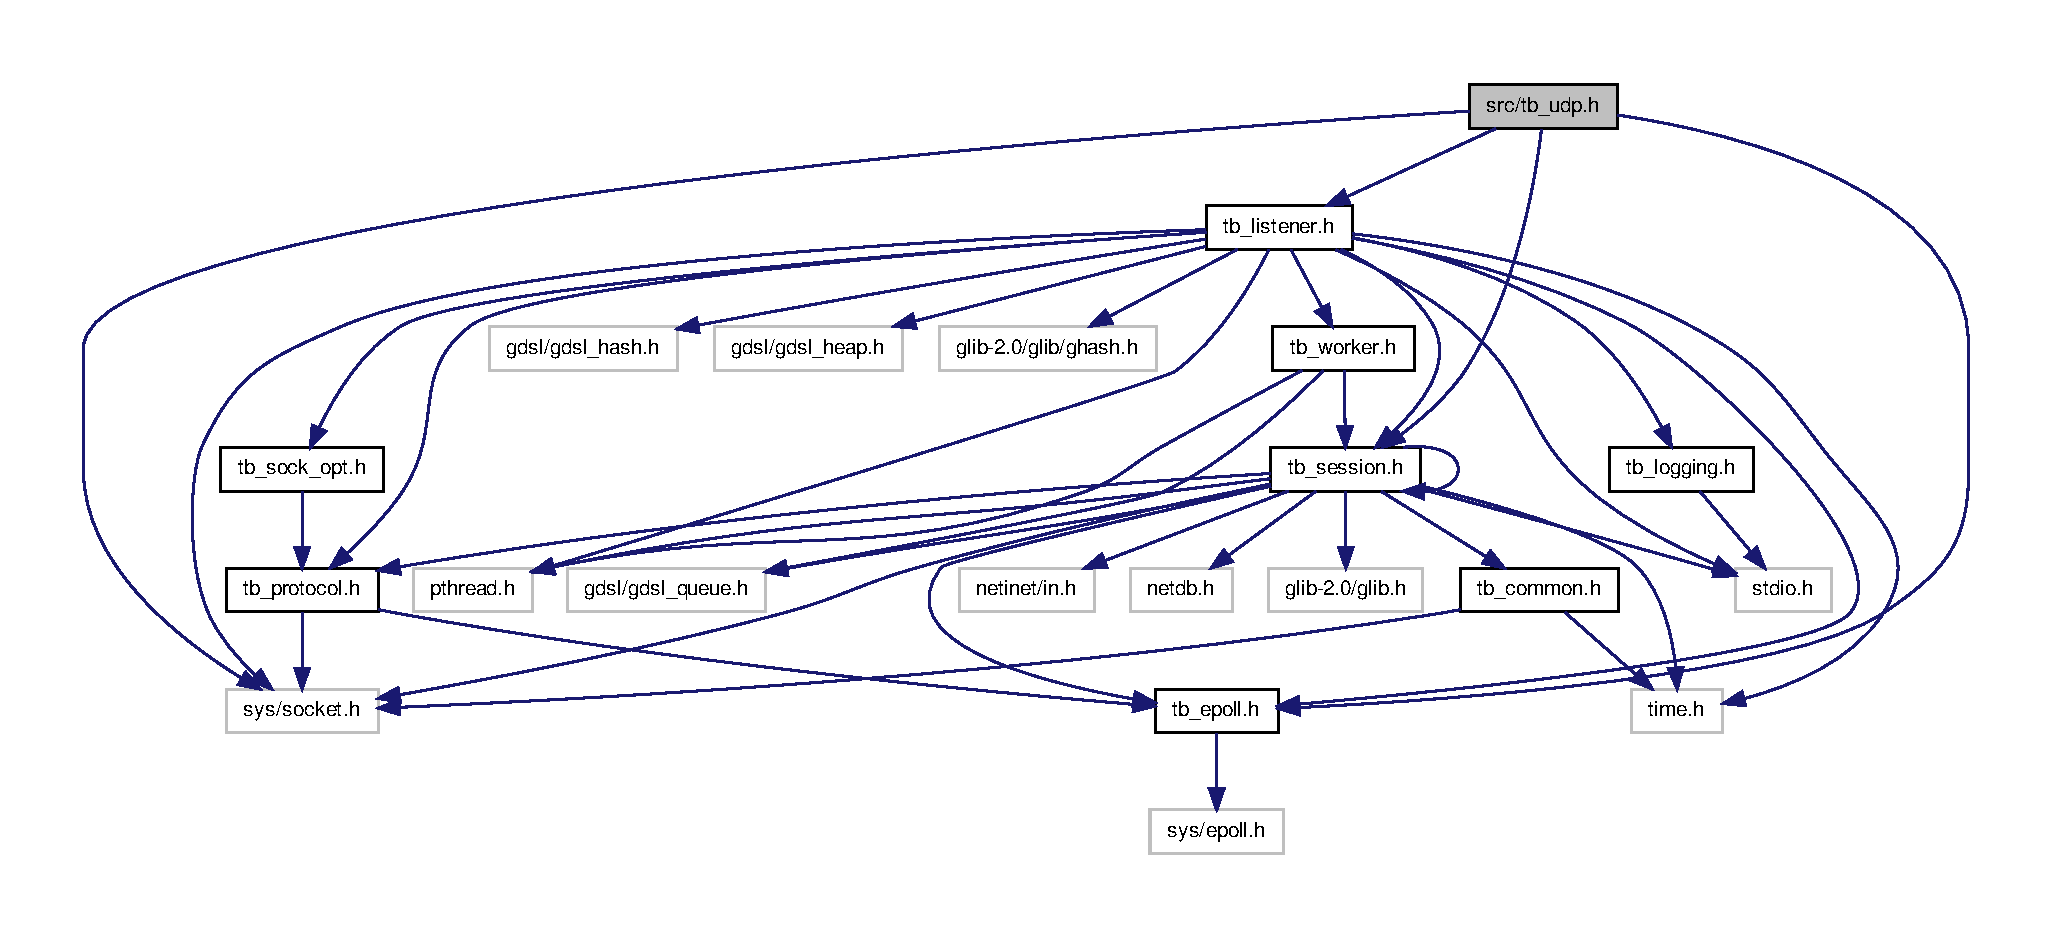
\includegraphics[width=350pt]{tb__udp_8h__incl}
\end{center}
\end{figure}
This graph shows which files directly or indirectly include this file\-:\nopagebreak
\begin{figure}[H]
\begin{center}
\leavevmode
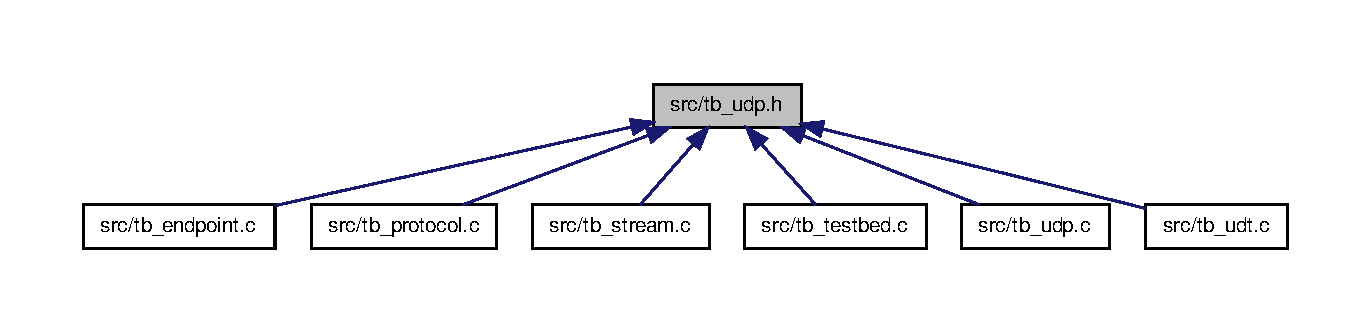
\includegraphics[width=350pt]{tb__udp_8h__dep__incl}
\end{center}
\end{figure}
\subsection*{Functions}
\begin{DoxyCompactItemize}
\item 
int \hyperlink{tb__udp_8h_a2d630c38c6c37789b56d70a575a1eeb5}{tb\-\_\-udp\-\_\-client} (\hyperlink{structtb__listener__t}{tb\-\_\-listener\-\_\-t} $\ast$listener)
\begin{DoxyCompactList}\small\item\em Upload a file using udp with epoll eof ack. \end{DoxyCompactList}\item 
int \hyperlink{tb__udp_8h_ac1be4ad75f9aa84b62a3cd530f822ea9}{tb\-\_\-udp\-\_\-ack} (int events, void $\ast$data)
\begin{DoxyCompactList}\small\item\em Callback function for udp. \end{DoxyCompactList}\item 
int \hyperlink{tb__udp_8h_a0e726d76f273fe0f7d77d569bbe481c0}{tb\-\_\-udp\-\_\-epoll\-\_\-client} (\hyperlink{structtb__listener__t}{tb\-\_\-listener\-\_\-t} $\ast$listener)
\begin{DoxyCompactList}\small\item\em Uses epoll for receiving data from the client. This is a prototype for T\-B0.\-2. \end{DoxyCompactList}\item 
int \hyperlink{tb__udp_8h_afeff69617372c952496e9cfebc707e1b}{tb\-\_\-udp\-\_\-m\-\_\-client} (\hyperlink{structtb__listener__t}{tb\-\_\-listener\-\_\-t} $\ast$listener)
\begin{DoxyCompactList}\small\item\em Called to create and start a udp client. \end{DoxyCompactList}\item 
int \hyperlink{tb__udp_8h_aa96de8208d00dd816bee9110ba759cf6}{tb\-\_\-udp\-\_\-server} (\hyperlink{structtb__listener__t}{tb\-\_\-listener\-\_\-t} $\ast$listener)
\begin{DoxyCompactList}\small\item\em Run a server using U\-D\-P, and epoll to signal transmission end. \end{DoxyCompactList}\item 
int \hyperlink{tb__udp_8h_a41ddaa85e718fa4afe65a979a58d7f9a}{tb\-\_\-udp\-\_\-epoll\-\_\-server} (\hyperlink{structtb__listener__t}{tb\-\_\-listener\-\_\-t} $\ast$listener)
\begin{DoxyCompactList}\small\item\em Run a server using epoll (non-\/blocking socket). \end{DoxyCompactList}\item 
int \hyperlink{tb__udp_8h_addeac1e739425f69c48947bab5e45436}{tb\-\_\-udp\-\_\-m\-\_\-server} (\hyperlink{structtb__listener__t}{tb\-\_\-listener\-\_\-t} $\ast$listener)
\begin{DoxyCompactList}\small\item\em Called to create and start a udp server. \end{DoxyCompactList}\item 
int \hyperlink{tb__udp_8h_a2b02206ecfea0b9f93e2ee1797436a04}{tb\-\_\-udp\-\_\-event} (int events, void $\ast$data)
\begin{DoxyCompactList}\small\item\em Epoll events function. \end{DoxyCompactList}\end{DoxyCompactItemize}


\subsection{Function Documentation}
\hypertarget{tb__udp_8h_ac1be4ad75f9aa84b62a3cd530f822ea9}{\index{tb\-\_\-udp.\-h@{tb\-\_\-udp.\-h}!tb\-\_\-udp\-\_\-ack@{tb\-\_\-udp\-\_\-ack}}
\index{tb\-\_\-udp\-\_\-ack@{tb\-\_\-udp\-\_\-ack}!tb_udp.h@{tb\-\_\-udp.\-h}}
\subsubsection[{tb\-\_\-udp\-\_\-ack}]{\setlength{\rightskip}{0pt plus 5cm}int tb\-\_\-udp\-\_\-ack (
\begin{DoxyParamCaption}
\item[{int}]{events, }
\item[{void $\ast$}]{data}
\end{DoxyParamCaption}
)}}\label{tb__udp_8h_ac1be4ad75f9aa84b62a3cd530f822ea9}


Callback function for udp. 

This is the function that is called when the eof from the server has be acknowledged. 

Definition at line 105 of file tb\-\_\-udp.\-c.

\hypertarget{tb__udp_8h_a2d630c38c6c37789b56d70a575a1eeb5}{\index{tb\-\_\-udp.\-h@{tb\-\_\-udp.\-h}!tb\-\_\-udp\-\_\-client@{tb\-\_\-udp\-\_\-client}}
\index{tb\-\_\-udp\-\_\-client@{tb\-\_\-udp\-\_\-client}!tb_udp.h@{tb\-\_\-udp.\-h}}
\subsubsection[{tb\-\_\-udp\-\_\-client}]{\setlength{\rightskip}{0pt plus 5cm}int tb\-\_\-udp\-\_\-client (
\begin{DoxyParamCaption}
\item[{{\bf tb\-\_\-listener\-\_\-t} $\ast$}]{listener}
\end{DoxyParamCaption}
)}}\label{tb__udp_8h_a2d630c38c6c37789b56d70a575a1eeb5}


Upload a file using udp with epoll eof ack. 

The difference between upload\-\_\-random\-\_\-udp and udp is that this uses the epoll mechanism to listenen for an ack of the eof. This insures that transmission is complete in the event of packet loss. 

Definition at line 37 of file tb\-\_\-udp.\-c.

\hypertarget{tb__udp_8h_a0e726d76f273fe0f7d77d569bbe481c0}{\index{tb\-\_\-udp.\-h@{tb\-\_\-udp.\-h}!tb\-\_\-udp\-\_\-epoll\-\_\-client@{tb\-\_\-udp\-\_\-epoll\-\_\-client}}
\index{tb\-\_\-udp\-\_\-epoll\-\_\-client@{tb\-\_\-udp\-\_\-epoll\-\_\-client}!tb_udp.h@{tb\-\_\-udp.\-h}}
\subsubsection[{tb\-\_\-udp\-\_\-epoll\-\_\-client}]{\setlength{\rightskip}{0pt plus 5cm}int tb\-\_\-udp\-\_\-epoll\-\_\-client (
\begin{DoxyParamCaption}
\item[{{\bf tb\-\_\-listener\-\_\-t} $\ast$}]{listener}
\end{DoxyParamCaption}
)}}\label{tb__udp_8h_a0e726d76f273fe0f7d77d569bbe481c0}


Uses epoll for receiving data from the client. This is a prototype for T\-B0.\-2. 



Definition at line 117 of file tb\-\_\-udp.\-c.

\hypertarget{tb__udp_8h_a41ddaa85e718fa4afe65a979a58d7f9a}{\index{tb\-\_\-udp.\-h@{tb\-\_\-udp.\-h}!tb\-\_\-udp\-\_\-epoll\-\_\-server@{tb\-\_\-udp\-\_\-epoll\-\_\-server}}
\index{tb\-\_\-udp\-\_\-epoll\-\_\-server@{tb\-\_\-udp\-\_\-epoll\-\_\-server}!tb_udp.h@{tb\-\_\-udp.\-h}}
\subsubsection[{tb\-\_\-udp\-\_\-epoll\-\_\-server}]{\setlength{\rightskip}{0pt plus 5cm}int tb\-\_\-udp\-\_\-epoll\-\_\-server (
\begin{DoxyParamCaption}
\item[{{\bf tb\-\_\-listener\-\_\-t} $\ast$}]{listener}
\end{DoxyParamCaption}
)}}\label{tb__udp_8h_a41ddaa85e718fa4afe65a979a58d7f9a}


Run a server using epoll (non-\/blocking socket). 

Runs a server that uses a sockets based protocol using epoll. Not used by U\-D\-T, a\-U\-D\-T or any thing else not implemented in sockets.


\begin{DoxyParams}{Parameters}
{\em listener} & The listener to run the server with. \\
\hline
\end{DoxyParams}


Definition at line 229 of file tb\-\_\-udp.\-c.

\hypertarget{tb__udp_8h_a2b02206ecfea0b9f93e2ee1797436a04}{\index{tb\-\_\-udp.\-h@{tb\-\_\-udp.\-h}!tb\-\_\-udp\-\_\-event@{tb\-\_\-udp\-\_\-event}}
\index{tb\-\_\-udp\-\_\-event@{tb\-\_\-udp\-\_\-event}!tb_udp.h@{tb\-\_\-udp.\-h}}
\subsubsection[{tb\-\_\-udp\-\_\-event}]{\setlength{\rightskip}{0pt plus 5cm}int tb\-\_\-udp\-\_\-event (
\begin{DoxyParamCaption}
\item[{int}]{events, }
\item[{void $\ast$}]{data}
\end{DoxyParamCaption}
)}}\label{tb__udp_8h_a2b02206ecfea0b9f93e2ee1797436a04}


Epoll events function. 

This is called when events occur on sockets that are polled by epoll. Processes incoming data. 

Definition at line 269 of file tb\-\_\-udp.\-c.

\hypertarget{tb__udp_8h_afeff69617372c952496e9cfebc707e1b}{\index{tb\-\_\-udp.\-h@{tb\-\_\-udp.\-h}!tb\-\_\-udp\-\_\-m\-\_\-client@{tb\-\_\-udp\-\_\-m\-\_\-client}}
\index{tb\-\_\-udp\-\_\-m\-\_\-client@{tb\-\_\-udp\-\_\-m\-\_\-client}!tb_udp.h@{tb\-\_\-udp.\-h}}
\subsubsection[{tb\-\_\-udp\-\_\-m\-\_\-client}]{\setlength{\rightskip}{0pt plus 5cm}int tb\-\_\-udp\-\_\-m\-\_\-client (
\begin{DoxyParamCaption}
\item[{{\bf tb\-\_\-listener\-\_\-t} $\ast$}]{listener}
\end{DoxyParamCaption}
)}}\label{tb__udp_8h_afeff69617372c952496e9cfebc707e1b}


Called to create and start a udp client. 



Definition at line 134 of file tb\-\_\-udp.\-c.

\hypertarget{tb__udp_8h_addeac1e739425f69c48947bab5e45436}{\index{tb\-\_\-udp.\-h@{tb\-\_\-udp.\-h}!tb\-\_\-udp\-\_\-m\-\_\-server@{tb\-\_\-udp\-\_\-m\-\_\-server}}
\index{tb\-\_\-udp\-\_\-m\-\_\-server@{tb\-\_\-udp\-\_\-m\-\_\-server}!tb_udp.h@{tb\-\_\-udp.\-h}}
\subsubsection[{tb\-\_\-udp\-\_\-m\-\_\-server}]{\setlength{\rightskip}{0pt plus 5cm}int tb\-\_\-udp\-\_\-m\-\_\-server (
\begin{DoxyParamCaption}
\item[{{\bf tb\-\_\-listener\-\_\-t} $\ast$}]{listener}
\end{DoxyParamCaption}
)}}\label{tb__udp_8h_addeac1e739425f69c48947bab5e45436}


Called to create and start a udp server. 



Definition at line 253 of file tb\-\_\-udp.\-c.

\hypertarget{tb__udp_8h_aa96de8208d00dd816bee9110ba759cf6}{\index{tb\-\_\-udp.\-h@{tb\-\_\-udp.\-h}!tb\-\_\-udp\-\_\-server@{tb\-\_\-udp\-\_\-server}}
\index{tb\-\_\-udp\-\_\-server@{tb\-\_\-udp\-\_\-server}!tb_udp.h@{tb\-\_\-udp.\-h}}
\subsubsection[{tb\-\_\-udp\-\_\-server}]{\setlength{\rightskip}{0pt plus 5cm}int tb\-\_\-udp\-\_\-server (
\begin{DoxyParamCaption}
\item[{{\bf tb\-\_\-listener\-\_\-t} $\ast$}]{listener}
\end{DoxyParamCaption}
)}}\label{tb__udp_8h_aa96de8208d00dd816bee9110ba759cf6}


Run a server using U\-D\-P, and epoll to signal transmission end. 



Definition at line 182 of file tb\-\_\-udp.\-c.


\hypertarget{tb__udt_8c}{\section{src/tb\-\_\-udt.c File Reference}
\label{tb__udt_8c}\index{src/tb\-\_\-udt.\-c@{src/tb\-\_\-udt.\-c}}
}
{\ttfamily \#include \char`\"{}tb\-\_\-udt.\-h\char`\"{}}\\*
{\ttfamily \#include \char`\"{}tb\-\_\-protocol.\-h\char`\"{}}\\*
{\ttfamily \#include \char`\"{}tb\-\_\-listener.\-h\char`\"{}}\\*
{\ttfamily \#include \char`\"{}tb\-\_\-testbed.\-h\char`\"{}}\\*
{\ttfamily \#include \char`\"{}tb\-\_\-common.\-h\char`\"{}}\\*
{\ttfamily \#include \char`\"{}tb\-\_\-udp.\-h\char`\"{}}\\*
{\ttfamily \#include \char`\"{}tb\-\_\-utp.\-h\char`\"{}}\\*
{\ttfamily \#include \char`\"{}udt.\-h\char`\"{}}\\*
{\ttfamily \#include \char`\"{}tb\-\_\-session.\-h\char`\"{}}\\*
{\ttfamily \#include \char`\"{}tb\-\_\-stream.\-h\char`\"{}}\\*
{\ttfamily \#include $<$utp.\-h$>$}\\*
{\ttfamily \#include $<$stdio.\-h$>$}\\*
{\ttfamily \#include $<$stdlib.\-h$>$}\\*
{\ttfamily \#include $<$assert.\-h$>$}\\*
{\ttfamily \#include $<$pthread.\-h$>$}\\*
{\ttfamily \#include $<$sys/socket.\-h$>$}\\*
{\ttfamily \#include $<$fcntl.\-h$>$}\\*
{\ttfamily \#include $<$unistd.\-h$>$}\\*
{\ttfamily \#include $<$string.\-h$>$}\\*
{\ttfamily \#include $<$sys/epoll.\-h$>$}\\*
{\ttfamily \#include $<$time.\-h$>$}\\*
{\ttfamily \#include $<$errno.\-h$>$}\\*
Include dependency graph for tb\-\_\-udt.\-c\-:\nopagebreak
\begin{figure}[H]
\begin{center}
\leavevmode
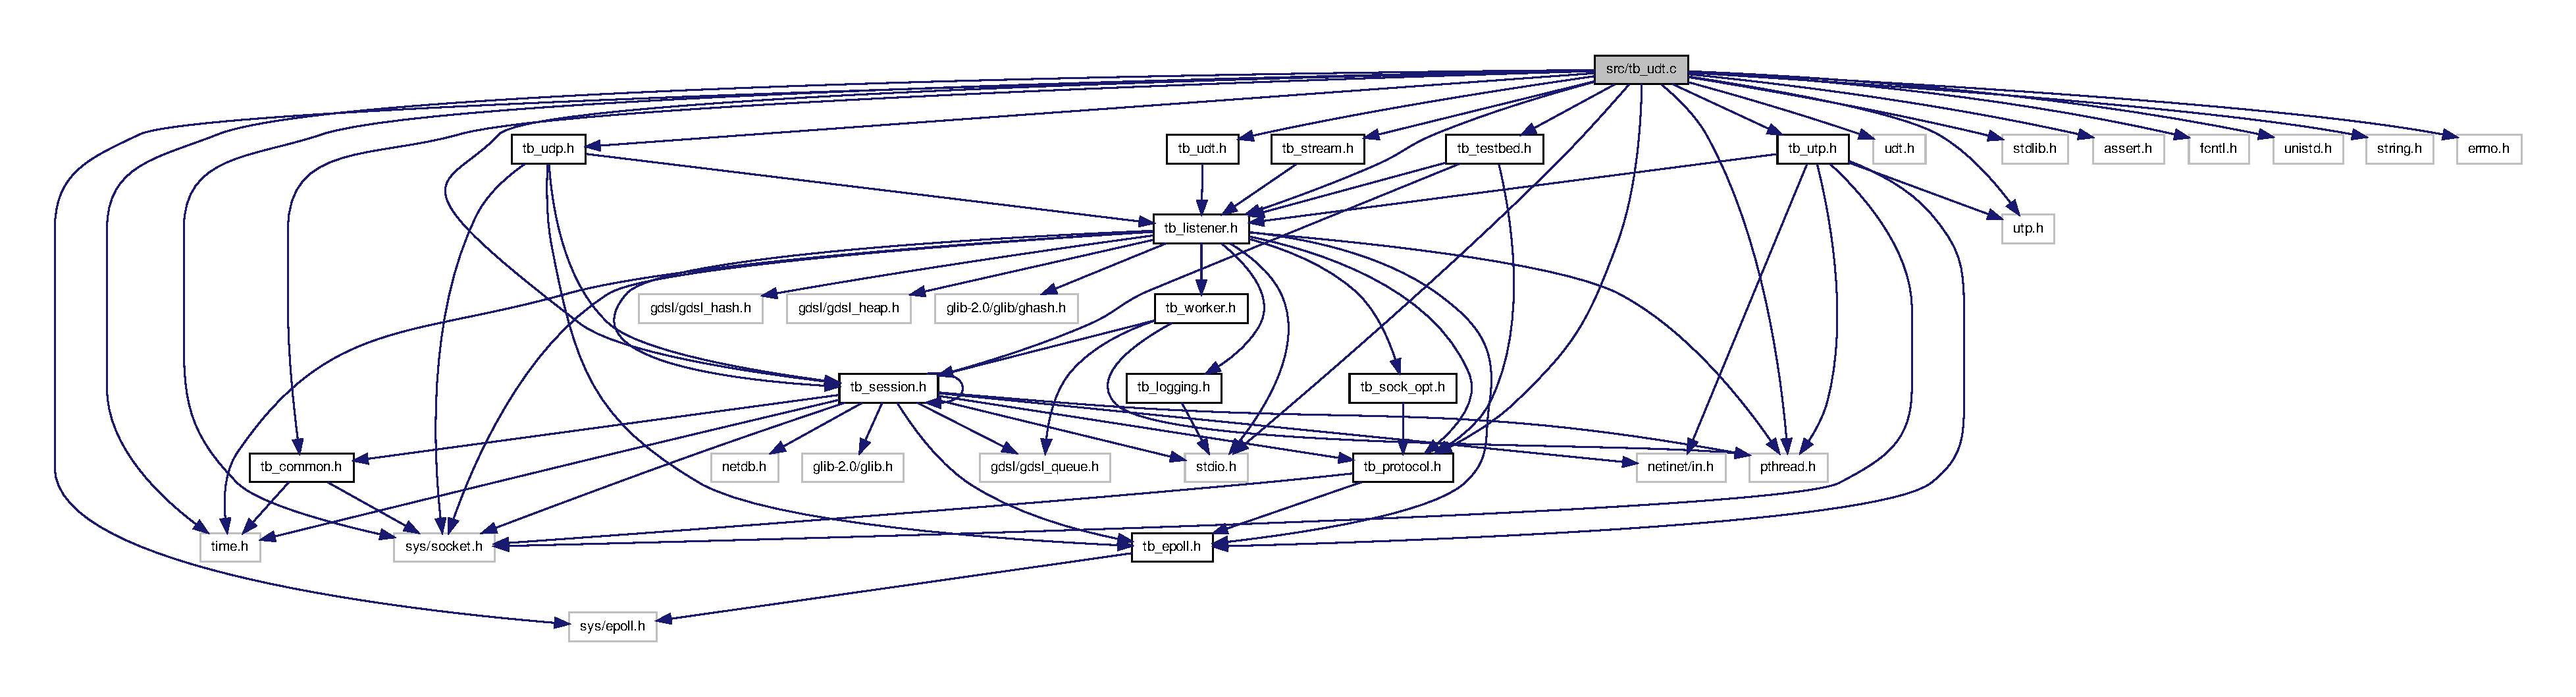
\includegraphics[width=350pt]{tb__udt_8c__incl}
\end{center}
\end{figure}
\subsection*{Functions}
\begin{DoxyCompactItemize}
\item 
int \hyperlink{tb__udt_8c_abbfc0a93f9d26ea48ce0f27f2341b25f}{tb\-\_\-udt\-\_\-server} (\hyperlink{structtb__listener__t}{tb\-\_\-listener\-\_\-t} $\ast$listener)
\begin{DoxyCompactList}\small\item\em Run the server with U\-D\-T. \end{DoxyCompactList}\item 
int \hyperlink{tb__udt_8c_a255780fa9ff0bbec144fa0d7cc884be7}{tb\-\_\-udt\-\_\-m\-\_\-server} (\hyperlink{structtb__listener__t}{tb\-\_\-listener\-\_\-t} $\ast$listener)
\begin{DoxyCompactList}\small\item\em Run a multi-\/connection server with U\-D\-T. \end{DoxyCompactList}\item 
int \hyperlink{tb__udt_8c_a30890790e001798fd4005d9d825a438c}{tb\-\_\-udt\-\_\-event} (\hyperlink{structtb__listener__t}{tb\-\_\-listener\-\_\-t} $\ast$listener)
\begin{DoxyCompactList}\small\item\em Accept a new incoming connection. \end{DoxyCompactList}\item 
void $\ast$ \hyperlink{tb__udt_8c_ab366fcad9034739ae6741115106b6777}{tb\-\_\-udt\-\_\-m\-\_\-server\-\_\-conn} (void $\ast$data)
\begin{DoxyCompactList}\small\item\em Read data from a connection. \end{DoxyCompactList}\item 
int \hyperlink{tb__udt_8c_a713f3ee749956d8e589263b56ddec118}{tb\-\_\-udt\-\_\-client} (\hyperlink{structtb__listener__t}{tb\-\_\-listener\-\_\-t} $\ast$listener)
\begin{DoxyCompactList}\small\item\em Upload a file using udt. \end{DoxyCompactList}\item 
int \hyperlink{tb__udt_8c_a11329d6c867c495bd2ac2dc04fdcc33b}{tb\-\_\-udt\-\_\-m\-\_\-client} (\hyperlink{structtb__listener__t}{tb\-\_\-listener\-\_\-t} $\ast$listener)
\begin{DoxyCompactList}\small\item\em Upload a file using multiple connections with U\-D\-T. \end{DoxyCompactList}\item 
void $\ast$ \hyperlink{tb__udt_8c_a848d2d8c3dcced0536cc607610007165}{tb\-\_\-udt\-\_\-m\-\_\-connection} (void $\ast$data)
\begin{DoxyCompactList}\small\item\em Write data to a connection. \end{DoxyCompactList}\end{DoxyCompactItemize}


\subsection{Function Documentation}
\hypertarget{tb__udt_8c_a713f3ee749956d8e589263b56ddec118}{\index{tb\-\_\-udt.\-c@{tb\-\_\-udt.\-c}!tb\-\_\-udt\-\_\-client@{tb\-\_\-udt\-\_\-client}}
\index{tb\-\_\-udt\-\_\-client@{tb\-\_\-udt\-\_\-client}!tb_udt.c@{tb\-\_\-udt.\-c}}
\subsubsection[{tb\-\_\-udt\-\_\-client}]{\setlength{\rightskip}{0pt plus 5cm}int tb\-\_\-udt\-\_\-client (
\begin{DoxyParamCaption}
\item[{{\bf tb\-\_\-listener\-\_\-t} $\ast$}]{listener}
\end{DoxyParamCaption}
)}}\label{tb__udt_8c_a713f3ee749956d8e589263b56ddec118}


Upload a file using udt. 



Definition at line 264 of file tb\-\_\-udt.\-c.

\hypertarget{tb__udt_8c_a30890790e001798fd4005d9d825a438c}{\index{tb\-\_\-udt.\-c@{tb\-\_\-udt.\-c}!tb\-\_\-udt\-\_\-event@{tb\-\_\-udt\-\_\-event}}
\index{tb\-\_\-udt\-\_\-event@{tb\-\_\-udt\-\_\-event}!tb_udt.c@{tb\-\_\-udt.\-c}}
\subsubsection[{tb\-\_\-udt\-\_\-event}]{\setlength{\rightskip}{0pt plus 5cm}int tb\-\_\-udt\-\_\-event (
\begin{DoxyParamCaption}
\item[{{\bf tb\-\_\-listener\-\_\-t} $\ast$}]{listener}
\end{DoxyParamCaption}
)}}\label{tb__udt_8c_a30890790e001798fd4005d9d825a438c}


Accept a new incoming connection. 

Called when udt\-\_\-epolls\-\_\-wait2 indicates that a new incoming connection is being made. 

Definition at line 180 of file tb\-\_\-udt.\-c.

\hypertarget{tb__udt_8c_a11329d6c867c495bd2ac2dc04fdcc33b}{\index{tb\-\_\-udt.\-c@{tb\-\_\-udt.\-c}!tb\-\_\-udt\-\_\-m\-\_\-client@{tb\-\_\-udt\-\_\-m\-\_\-client}}
\index{tb\-\_\-udt\-\_\-m\-\_\-client@{tb\-\_\-udt\-\_\-m\-\_\-client}!tb_udt.c@{tb\-\_\-udt.\-c}}
\subsubsection[{tb\-\_\-udt\-\_\-m\-\_\-client}]{\setlength{\rightskip}{0pt plus 5cm}int tb\-\_\-udt\-\_\-m\-\_\-client (
\begin{DoxyParamCaption}
\item[{{\bf tb\-\_\-listener\-\_\-t} $\ast$}]{listener}
\end{DoxyParamCaption}
)}}\label{tb__udt_8c_a11329d6c867c495bd2ac2dc04fdcc33b}


Upload a file using multiple connections with U\-D\-T. 

Uses multiple connections to upload files using the U\-D\-T protocol. The number of connections to be used is stored in the num\-\_\-connections field in \hyperlink{structtb__listener__t}{tb\-\_\-listener\-\_\-t}.


\begin{DoxyParams}{Parameters}
{\em listener} & A vaild \hyperlink{structtb__listener__t}{tb\-\_\-listener\-\_\-t} struct, with connection data. \\
\hline
\end{DoxyParams}


Definition at line 308 of file tb\-\_\-udt.\-c.

\hypertarget{tb__udt_8c_a848d2d8c3dcced0536cc607610007165}{\index{tb\-\_\-udt.\-c@{tb\-\_\-udt.\-c}!tb\-\_\-udt\-\_\-m\-\_\-connection@{tb\-\_\-udt\-\_\-m\-\_\-connection}}
\index{tb\-\_\-udt\-\_\-m\-\_\-connection@{tb\-\_\-udt\-\_\-m\-\_\-connection}!tb_udt.c@{tb\-\_\-udt.\-c}}
\subsubsection[{tb\-\_\-udt\-\_\-m\-\_\-connection}]{\setlength{\rightskip}{0pt plus 5cm}void$\ast$ tb\-\_\-udt\-\_\-m\-\_\-connection (
\begin{DoxyParamCaption}
\item[{void $\ast$}]{data}
\end{DoxyParamCaption}
)}}\label{tb__udt_8c_a848d2d8c3dcced0536cc607610007165}


Write data to a connection. 

Called when creating new client connections to multi-\/connection servers. Passed as a function pointer to pthread\-\_\-create. 

Definition at line 383 of file tb\-\_\-udt.\-c.

\hypertarget{tb__udt_8c_a255780fa9ff0bbec144fa0d7cc884be7}{\index{tb\-\_\-udt.\-c@{tb\-\_\-udt.\-c}!tb\-\_\-udt\-\_\-m\-\_\-server@{tb\-\_\-udt\-\_\-m\-\_\-server}}
\index{tb\-\_\-udt\-\_\-m\-\_\-server@{tb\-\_\-udt\-\_\-m\-\_\-server}!tb_udt.c@{tb\-\_\-udt.\-c}}
\subsubsection[{tb\-\_\-udt\-\_\-m\-\_\-server}]{\setlength{\rightskip}{0pt plus 5cm}int tb\-\_\-udt\-\_\-m\-\_\-server (
\begin{DoxyParamCaption}
\item[{{\bf tb\-\_\-listener\-\_\-t} $\ast$}]{listener}
\end{DoxyParamCaption}
)}}\label{tb__udt_8c_a255780fa9ff0bbec144fa0d7cc884be7}


Run a multi-\/connection server with U\-D\-T. 

Runs a server that can handle multiple connections using the U\-D\-T protocol. 

Definition at line 128 of file tb\-\_\-udt.\-c.

\hypertarget{tb__udt_8c_ab366fcad9034739ae6741115106b6777}{\index{tb\-\_\-udt.\-c@{tb\-\_\-udt.\-c}!tb\-\_\-udt\-\_\-m\-\_\-server\-\_\-conn@{tb\-\_\-udt\-\_\-m\-\_\-server\-\_\-conn}}
\index{tb\-\_\-udt\-\_\-m\-\_\-server\-\_\-conn@{tb\-\_\-udt\-\_\-m\-\_\-server\-\_\-conn}!tb_udt.c@{tb\-\_\-udt.\-c}}
\subsubsection[{tb\-\_\-udt\-\_\-m\-\_\-server\-\_\-conn}]{\setlength{\rightskip}{0pt plus 5cm}void$\ast$ tb\-\_\-udt\-\_\-m\-\_\-server\-\_\-conn (
\begin{DoxyParamCaption}
\item[{void $\ast$}]{data}
\end{DoxyParamCaption}
)}}\label{tb__udt_8c_ab366fcad9034739ae6741115106b6777}


Read data from a connection. 

Called to read data from a new connection. Passed in as a function pointer in the pthread\-\_\-create function is called.

\begin{DoxyPrecond}{Precondition}
data must be a \hyperlink{structtb__session__t}{tb\-\_\-session\-\_\-t} struct. 
\end{DoxyPrecond}

\begin{DoxyParams}{Parameters}
{\em data} & void pointer to a \hyperlink{structtb__session__t}{tb\-\_\-session\-\_\-t} struct. \\
\hline
\end{DoxyParams}
\begin{DoxyReturn}{Returns}
pointer to int, 0 if connection terminated normally, -\/1 if not. 
\end{DoxyReturn}


Definition at line 221 of file tb\-\_\-udt.\-c.

\hypertarget{tb__udt_8c_abbfc0a93f9d26ea48ce0f27f2341b25f}{\index{tb\-\_\-udt.\-c@{tb\-\_\-udt.\-c}!tb\-\_\-udt\-\_\-server@{tb\-\_\-udt\-\_\-server}}
\index{tb\-\_\-udt\-\_\-server@{tb\-\_\-udt\-\_\-server}!tb_udt.c@{tb\-\_\-udt.\-c}}
\subsubsection[{tb\-\_\-udt\-\_\-server}]{\setlength{\rightskip}{0pt plus 5cm}int tb\-\_\-udt\-\_\-server (
\begin{DoxyParamCaption}
\item[{{\bf tb\-\_\-listener\-\_\-t} $\ast$}]{listener}
\end{DoxyParamCaption}
)}}\label{tb__udt_8c_abbfc0a93f9d26ea48ce0f27f2341b25f}


Run the server with U\-D\-T. 

This runs the T\-B server with the U\-D\-T protocol.


\begin{DoxyParams}{Parameters}
{\em listener} & The listener to run with. \\
\hline
\end{DoxyParams}


Definition at line 37 of file tb\-\_\-udt.\-c.


\hypertarget{tb__udt_8h}{\section{src/tb\-\_\-udt.h File Reference}
\label{tb__udt_8h}\index{src/tb\-\_\-udt.\-h@{src/tb\-\_\-udt.\-h}}
}
{\ttfamily \#include \char`\"{}tb\-\_\-listener.\-h\char`\"{}}\\*
Include dependency graph for tb\-\_\-udt.\-h\-:\nopagebreak
\begin{figure}[H]
\begin{center}
\leavevmode
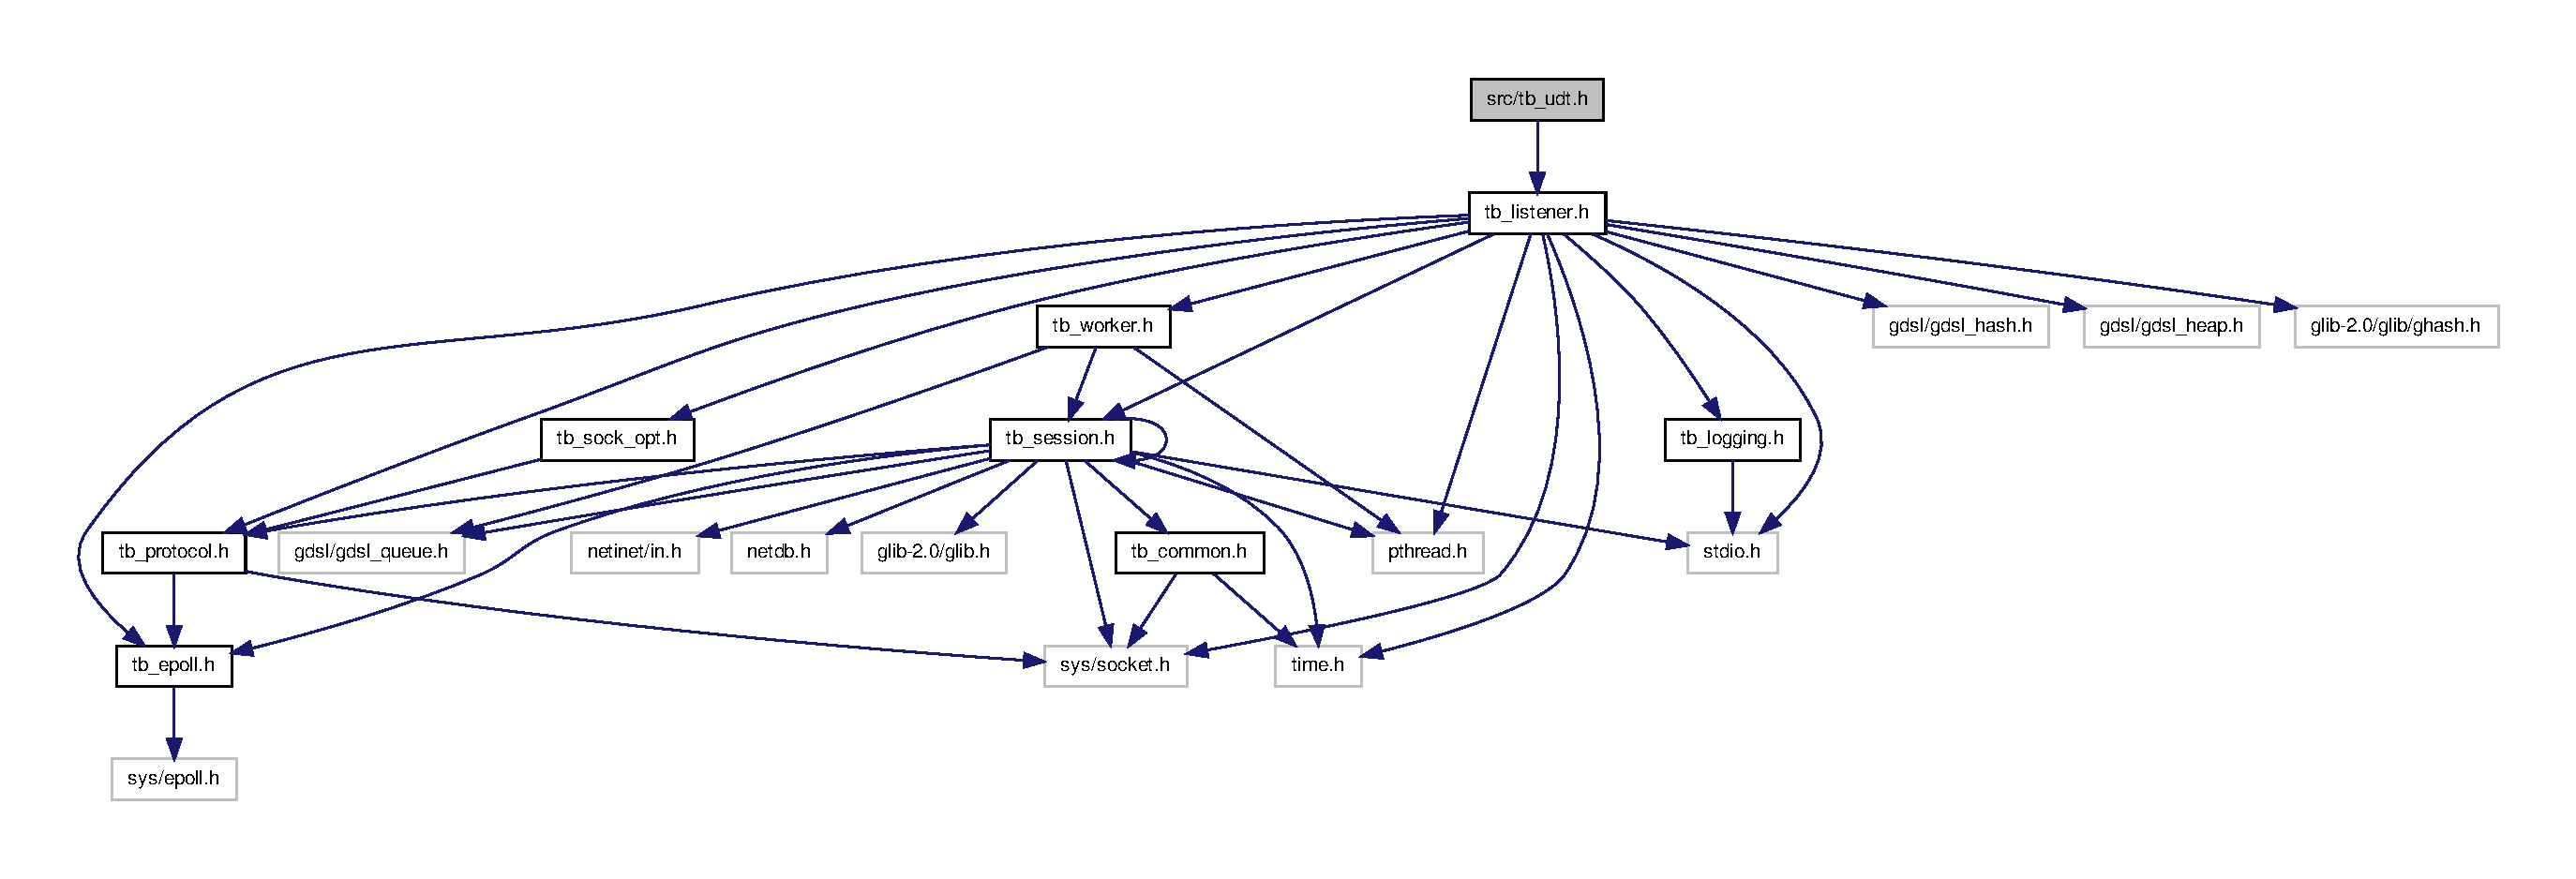
\includegraphics[width=350pt]{tb__udt_8h__incl}
\end{center}
\end{figure}
This graph shows which files directly or indirectly include this file\-:\nopagebreak
\begin{figure}[H]
\begin{center}
\leavevmode
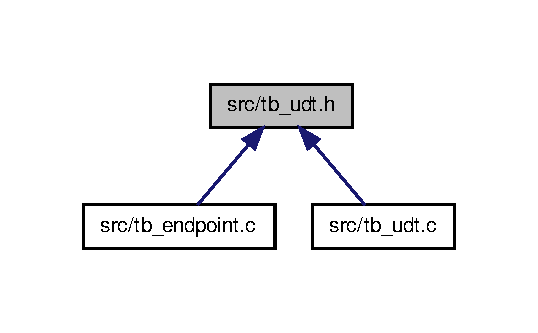
\includegraphics[width=258pt]{tb__udt_8h__dep__incl}
\end{center}
\end{figure}
\subsection*{Functions}
\begin{DoxyCompactItemize}
\item 
int \hyperlink{tb__udt_8h_abbfc0a93f9d26ea48ce0f27f2341b25f}{tb\-\_\-udt\-\_\-server} (\hyperlink{structtb__listener__t}{tb\-\_\-listener\-\_\-t} $\ast$listener)
\begin{DoxyCompactList}\small\item\em Run the server with U\-D\-T. \end{DoxyCompactList}\item 
int \hyperlink{tb__udt_8h_a255780fa9ff0bbec144fa0d7cc884be7}{tb\-\_\-udt\-\_\-m\-\_\-server} (\hyperlink{structtb__listener__t}{tb\-\_\-listener\-\_\-t} $\ast$listener)
\begin{DoxyCompactList}\small\item\em Run a multi-\/connection server with U\-D\-T. \end{DoxyCompactList}\item 
int \hyperlink{tb__udt_8h_a30890790e001798fd4005d9d825a438c}{tb\-\_\-udt\-\_\-event} (\hyperlink{structtb__listener__t}{tb\-\_\-listener\-\_\-t} $\ast$listener)
\begin{DoxyCompactList}\small\item\em Accept a new incoming connection. \end{DoxyCompactList}\item 
void $\ast$ \hyperlink{tb__udt_8h_ab366fcad9034739ae6741115106b6777}{tb\-\_\-udt\-\_\-m\-\_\-server\-\_\-conn} (void $\ast$data)
\begin{DoxyCompactList}\small\item\em Read data from a connection. \end{DoxyCompactList}\item 
int \hyperlink{tb__udt_8h_a713f3ee749956d8e589263b56ddec118}{tb\-\_\-udt\-\_\-client} (\hyperlink{structtb__listener__t}{tb\-\_\-listener\-\_\-t} $\ast$listener)
\begin{DoxyCompactList}\small\item\em Upload a file using udt. \end{DoxyCompactList}\item 
int \hyperlink{tb__udt_8h_a11329d6c867c495bd2ac2dc04fdcc33b}{tb\-\_\-udt\-\_\-m\-\_\-client} (\hyperlink{structtb__listener__t}{tb\-\_\-listener\-\_\-t} $\ast$listener)
\begin{DoxyCompactList}\small\item\em Upload a file using multiple connections with U\-D\-T. \end{DoxyCompactList}\item 
void $\ast$ \hyperlink{tb__udt_8h_a848d2d8c3dcced0536cc607610007165}{tb\-\_\-udt\-\_\-m\-\_\-connection} (void $\ast$data)
\begin{DoxyCompactList}\small\item\em Write data to a connection. \end{DoxyCompactList}\end{DoxyCompactItemize}


\subsection{Function Documentation}
\hypertarget{tb__udt_8h_a713f3ee749956d8e589263b56ddec118}{\index{tb\-\_\-udt.\-h@{tb\-\_\-udt.\-h}!tb\-\_\-udt\-\_\-client@{tb\-\_\-udt\-\_\-client}}
\index{tb\-\_\-udt\-\_\-client@{tb\-\_\-udt\-\_\-client}!tb_udt.h@{tb\-\_\-udt.\-h}}
\subsubsection[{tb\-\_\-udt\-\_\-client}]{\setlength{\rightskip}{0pt plus 5cm}int tb\-\_\-udt\-\_\-client (
\begin{DoxyParamCaption}
\item[{{\bf tb\-\_\-listener\-\_\-t} $\ast$}]{listener}
\end{DoxyParamCaption}
)}}\label{tb__udt_8h_a713f3ee749956d8e589263b56ddec118}


Upload a file using udt. 



Definition at line 264 of file tb\-\_\-udt.\-c.

\hypertarget{tb__udt_8h_a30890790e001798fd4005d9d825a438c}{\index{tb\-\_\-udt.\-h@{tb\-\_\-udt.\-h}!tb\-\_\-udt\-\_\-event@{tb\-\_\-udt\-\_\-event}}
\index{tb\-\_\-udt\-\_\-event@{tb\-\_\-udt\-\_\-event}!tb_udt.h@{tb\-\_\-udt.\-h}}
\subsubsection[{tb\-\_\-udt\-\_\-event}]{\setlength{\rightskip}{0pt plus 5cm}int tb\-\_\-udt\-\_\-event (
\begin{DoxyParamCaption}
\item[{{\bf tb\-\_\-listener\-\_\-t} $\ast$}]{listener}
\end{DoxyParamCaption}
)}}\label{tb__udt_8h_a30890790e001798fd4005d9d825a438c}


Accept a new incoming connection. 

Called when udt\-\_\-epolls\-\_\-wait2 indicates that a new incoming connection is being made. 

Definition at line 180 of file tb\-\_\-udt.\-c.

\hypertarget{tb__udt_8h_a11329d6c867c495bd2ac2dc04fdcc33b}{\index{tb\-\_\-udt.\-h@{tb\-\_\-udt.\-h}!tb\-\_\-udt\-\_\-m\-\_\-client@{tb\-\_\-udt\-\_\-m\-\_\-client}}
\index{tb\-\_\-udt\-\_\-m\-\_\-client@{tb\-\_\-udt\-\_\-m\-\_\-client}!tb_udt.h@{tb\-\_\-udt.\-h}}
\subsubsection[{tb\-\_\-udt\-\_\-m\-\_\-client}]{\setlength{\rightskip}{0pt plus 5cm}int tb\-\_\-udt\-\_\-m\-\_\-client (
\begin{DoxyParamCaption}
\item[{{\bf tb\-\_\-listener\-\_\-t} $\ast$}]{listener}
\end{DoxyParamCaption}
)}}\label{tb__udt_8h_a11329d6c867c495bd2ac2dc04fdcc33b}


Upload a file using multiple connections with U\-D\-T. 

Uses multiple connections to upload files using the U\-D\-T protocol. The number of connections to be used is stored in the num\-\_\-connections field in \hyperlink{structtb__listener__t}{tb\-\_\-listener\-\_\-t}.


\begin{DoxyParams}{Parameters}
{\em listener} & A vaild \hyperlink{structtb__listener__t}{tb\-\_\-listener\-\_\-t} struct, with connection data. \\
\hline
\end{DoxyParams}


Definition at line 308 of file tb\-\_\-udt.\-c.

\hypertarget{tb__udt_8h_a848d2d8c3dcced0536cc607610007165}{\index{tb\-\_\-udt.\-h@{tb\-\_\-udt.\-h}!tb\-\_\-udt\-\_\-m\-\_\-connection@{tb\-\_\-udt\-\_\-m\-\_\-connection}}
\index{tb\-\_\-udt\-\_\-m\-\_\-connection@{tb\-\_\-udt\-\_\-m\-\_\-connection}!tb_udt.h@{tb\-\_\-udt.\-h}}
\subsubsection[{tb\-\_\-udt\-\_\-m\-\_\-connection}]{\setlength{\rightskip}{0pt plus 5cm}void$\ast$ tb\-\_\-udt\-\_\-m\-\_\-connection (
\begin{DoxyParamCaption}
\item[{void $\ast$}]{data}
\end{DoxyParamCaption}
)}}\label{tb__udt_8h_a848d2d8c3dcced0536cc607610007165}


Write data to a connection. 

Called when creating new client connections to multi-\/connection servers. Passed as a function pointer to pthread\-\_\-create. 

Definition at line 383 of file tb\-\_\-udt.\-c.

\hypertarget{tb__udt_8h_a255780fa9ff0bbec144fa0d7cc884be7}{\index{tb\-\_\-udt.\-h@{tb\-\_\-udt.\-h}!tb\-\_\-udt\-\_\-m\-\_\-server@{tb\-\_\-udt\-\_\-m\-\_\-server}}
\index{tb\-\_\-udt\-\_\-m\-\_\-server@{tb\-\_\-udt\-\_\-m\-\_\-server}!tb_udt.h@{tb\-\_\-udt.\-h}}
\subsubsection[{tb\-\_\-udt\-\_\-m\-\_\-server}]{\setlength{\rightskip}{0pt plus 5cm}int tb\-\_\-udt\-\_\-m\-\_\-server (
\begin{DoxyParamCaption}
\item[{{\bf tb\-\_\-listener\-\_\-t} $\ast$}]{listener}
\end{DoxyParamCaption}
)}}\label{tb__udt_8h_a255780fa9ff0bbec144fa0d7cc884be7}


Run a multi-\/connection server with U\-D\-T. 

Runs a server that can handle multiple connections using the U\-D\-T protocol. 

Definition at line 128 of file tb\-\_\-udt.\-c.

\hypertarget{tb__udt_8h_ab366fcad9034739ae6741115106b6777}{\index{tb\-\_\-udt.\-h@{tb\-\_\-udt.\-h}!tb\-\_\-udt\-\_\-m\-\_\-server\-\_\-conn@{tb\-\_\-udt\-\_\-m\-\_\-server\-\_\-conn}}
\index{tb\-\_\-udt\-\_\-m\-\_\-server\-\_\-conn@{tb\-\_\-udt\-\_\-m\-\_\-server\-\_\-conn}!tb_udt.h@{tb\-\_\-udt.\-h}}
\subsubsection[{tb\-\_\-udt\-\_\-m\-\_\-server\-\_\-conn}]{\setlength{\rightskip}{0pt plus 5cm}void$\ast$ tb\-\_\-udt\-\_\-m\-\_\-server\-\_\-conn (
\begin{DoxyParamCaption}
\item[{void $\ast$}]{data}
\end{DoxyParamCaption}
)}}\label{tb__udt_8h_ab366fcad9034739ae6741115106b6777}


Read data from a connection. 

Called to read data from a new connection. Passed in as a function pointer in the pthread\-\_\-create function is called.

\begin{DoxyPrecond}{Precondition}
data must be a \hyperlink{structtb__session__t}{tb\-\_\-session\-\_\-t} struct. 
\end{DoxyPrecond}

\begin{DoxyParams}{Parameters}
{\em data} & void pointer to a \hyperlink{structtb__session__t}{tb\-\_\-session\-\_\-t} struct. \\
\hline
\end{DoxyParams}
\begin{DoxyReturn}{Returns}
pointer to int, 0 if connection terminated normally, -\/1 if not. 
\end{DoxyReturn}


Definition at line 221 of file tb\-\_\-udt.\-c.

\hypertarget{tb__udt_8h_abbfc0a93f9d26ea48ce0f27f2341b25f}{\index{tb\-\_\-udt.\-h@{tb\-\_\-udt.\-h}!tb\-\_\-udt\-\_\-server@{tb\-\_\-udt\-\_\-server}}
\index{tb\-\_\-udt\-\_\-server@{tb\-\_\-udt\-\_\-server}!tb_udt.h@{tb\-\_\-udt.\-h}}
\subsubsection[{tb\-\_\-udt\-\_\-server}]{\setlength{\rightskip}{0pt plus 5cm}int tb\-\_\-udt\-\_\-server (
\begin{DoxyParamCaption}
\item[{{\bf tb\-\_\-listener\-\_\-t} $\ast$}]{listener}
\end{DoxyParamCaption}
)}}\label{tb__udt_8h_abbfc0a93f9d26ea48ce0f27f2341b25f}


Run the server with U\-D\-T. 

This runs the T\-B server with the U\-D\-T protocol.


\begin{DoxyParams}{Parameters}
{\em listener} & The listener to run with. \\
\hline
\end{DoxyParams}


Definition at line 37 of file tb\-\_\-udt.\-c.


\hypertarget{tb__utp_8c}{\section{src/tb\-\_\-utp.c File Reference}
\label{tb__utp_8c}\index{src/tb\-\_\-utp.\-c@{src/tb\-\_\-utp.\-c}}
}
{\ttfamily \#include \char`\"{}tb\-\_\-utp.\-h\char`\"{}}\\*
{\ttfamily \#include \char`\"{}tb\-\_\-epoll.\-h\char`\"{}}\\*
{\ttfamily \#include \char`\"{}tb\-\_\-common.\-h\char`\"{}}\\*
{\ttfamily \#include \char`\"{}tb\-\_\-listener.\-h\char`\"{}}\\*
{\ttfamily \#include \char`\"{}tb\-\_\-testbed.\-h\char`\"{}}\\*
{\ttfamily \#include $<$utp.\-h$>$}\\*
{\ttfamily \#include $<$netinet/in.\-h$>$}\\*
{\ttfamily \#include $<$arpa/inet.\-h$>$}\\*
{\ttfamily \#include $<$stdlib.\-h$>$}\\*
{\ttfamily \#include $<$string.\-h$>$}\\*
{\ttfamily \#include $<$stdio.\-h$>$}\\*
{\ttfamily \#include $<$pthread.\-h$>$}\\*
{\ttfamily \#include $<$assert.\-h$>$}\\*
{\ttfamily \#include $<$sys/epoll.\-h$>$}\\*
{\ttfamily \#include $<$fcntl.\-h$>$}\\*
{\ttfamily \#include $<$netdb.\-h$>$}\\*
{\ttfamily \#include $<$sys/socket.\-h$>$}\\*
{\ttfamily \#include $<$sys/types.\-h$>$}\\*
{\ttfamily \#include $<$errno.\-h$>$}\\*
{\ttfamily \#include $<$unistd.\-h$>$}\\*
Include dependency graph for tb\-\_\-utp.\-c\-:\nopagebreak
\begin{figure}[H]
\begin{center}
\leavevmode
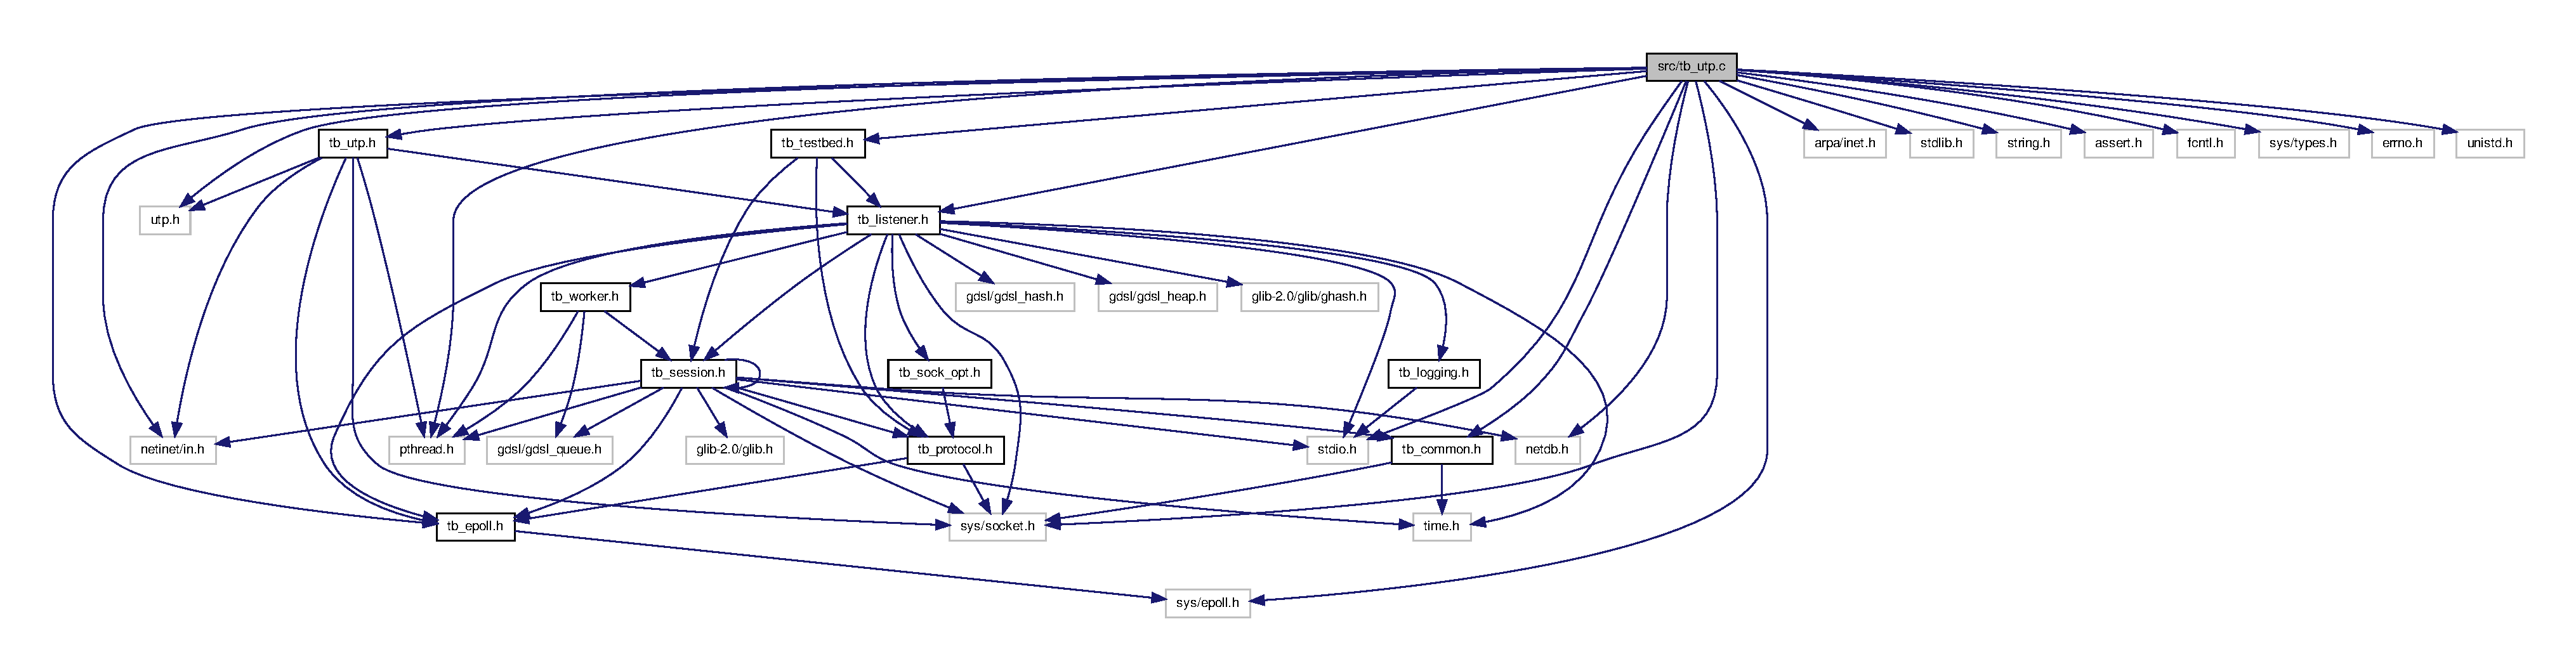
\includegraphics[width=350pt]{tb__utp_8c__incl}
\end{center}
\end{figure}
\subsection*{Functions}
\begin{DoxyCompactItemize}
\item 
\hyperlink{structtb__utp__t}{tb\-\_\-utp\-\_\-t} $\ast$ \hyperlink{tb__utp_8c_a506a49d3c557eba2fef9b778738743b6}{tb\-\_\-utp\-\_\-setup} ()
\item 
void \hyperlink{tb__utp_8c_a26220ca07feac95d0ebdccfaf0228f86}{tb\-\_\-utp\-\_\-read} (void $\ast$userdata, const byte $\ast$bytes, size\-\_\-t count)
\item 
void \hyperlink{tb__utp_8c_a435677dbfa73e419e5155d978ee893c4}{tb\-\_\-utp\-\_\-write} (void $\ast$userdata, byte $\ast$bytes, size\-\_\-t count)
\item 
size\-\_\-t \hyperlink{tb__utp_8c_a78dc4e9a5c6efe713d6bac1e968ce6f1}{tb\-\_\-utp\-\_\-get\-\_\-\-Rcv\-\_\-buff} (void $\ast$userdata)
\item 
void \hyperlink{tb__utp_8c_a1e25222015d067d9bfdf2046b27b58af}{tb\-\_\-utp\-\_\-state\-\_\-change} (void $\ast$userdata, int state)
\item 
void \hyperlink{tb__utp_8c_ab15274bd142f9d742f43ff8670eee3cd}{tb\-\_\-utp\-\_\-error} (void $\ast$userdata, int errcode)
\item 
void \hyperlink{tb__utp_8c_af31fb5ebecca7ed41d3b82654a6d57c6}{tb\-\_\-utp\-\_\-overhead} (void $\ast$userdata, int send, size\-\_\-t count, int type)
\item 
void \hyperlink{tb__utp_8c_a11b6cdd962696b52f2fcac93df1e28e3}{tb\-\_\-utp\-\_\-send\-\_\-to} (void $\ast$userdata, const byte $\ast$p, size\-\_\-t len, const struct sockaddr $\ast$to, socklen\-\_\-t tolen)
\item 
void \hyperlink{tb__utp_8c_a43444f296566ed304ac2934328dd20a0}{tb\-\_\-utp\-\_\-incoming} (void $\ast$userdata, struct U\-T\-P\-Socket $\ast$socket)
\begin{DoxyCompactList}\small\item\em callback, for incoming connections. \end{DoxyCompactList}\item 
int \hyperlink{tb__utp_8c_a07325129f2f67a976ddd914e71b67881}{tb\-\_\-utp\-\_\-socket} (\hyperlink{structtb__utp__t}{tb\-\_\-utp\-\_\-t} $\ast$utp, int domain, int socktype, int protocol)
\item 
int \hyperlink{tb__utp_8c_ae499f3155494fdc2ea5e53375c1ab5ed}{tb\-\_\-utp\-\_\-connect} (\hyperlink{structtb__utp__t}{tb\-\_\-utp\-\_\-t} $\ast$utp, const struct sockaddr $\ast$addr, socklen\-\_\-t len)
\item 
int \hyperlink{tb__utp_8c_a9dca05324926fb62deab6aa46f130696}{tb\-\_\-utp\-\_\-send} (\hyperlink{structtb__utp__t}{tb\-\_\-utp\-\_\-t} $\ast$utp, void $\ast$buf, size\-\_\-t n)
\item 
int \hyperlink{tb__utp_8c_a166ed93b320918ba496852d8e4b37059}{tb\-\_\-utp\-\_\-event} (int events, void $\ast$data)
\begin{DoxyCompactList}\small\item\em Callback used by epoll events. \end{DoxyCompactList}\item 
int \hyperlink{tb__utp_8c_a73863f08a2e18eb80fac12509f0ccaff}{tb\-\_\-utp\-\_\-recv} (\hyperlink{structtb__utp__t}{tb\-\_\-utp\-\_\-t} $\ast$utp, char $\ast$buff, int size)
\begin{DoxyCompactList}\small\item\em Receive data from a u\-T\-P socket. \end{DoxyCompactList}\item 
int \hyperlink{tb__utp_8c_a00c956cd2abf69fde14be69ff5e7aa0c}{tb\-\_\-utp\-\_\-funct\-\_\-exit} ()
\item 
int \hyperlink{tb__utp_8c_ab3bd87fbc20dbbd52543b2fab384f29f}{tb\-\_\-utp\-\_\-error\-\_\-handle} (int value, int err\-\_\-no)
\item 
int \hyperlink{tb__utp_8c_a914e27dc988c6efc694ad951dadefc6b}{tb\-\_\-utp\-\_\-close} (\hyperlink{structtb__utp__t}{tb\-\_\-utp\-\_\-t} $\ast$utp)
\item 
int \hyperlink{tb__utp_8c_aaef934c0644a4ded7635420534b2bd01}{tb\-\_\-utp\-\_\-client} (\hyperlink{structtb__listener__t}{tb\-\_\-listener\-\_\-t} $\ast$listener)
\begin{DoxyCompactList}\small\item\em Upload using the u\-T\-P protocol. \end{DoxyCompactList}\item 
int \hyperlink{tb__utp_8c_aacb2150e3f5d787a6d04e4c69663f643}{tb\-\_\-utp\-\_\-m\-\_\-server} (\hyperlink{structtb__listener__t}{tb\-\_\-listener\-\_\-t} $\ast$listener)
\begin{DoxyCompactList}\small\item\em Create a multiconnection server using u\-T\-P. \end{DoxyCompactList}\item 
int \hyperlink{tb__utp_8c_a91f1cecaee23c1889b8588111d17ddb1}{tb\-\_\-utp\-\_\-m\-\_\-event} (int events, void $\ast$data)
\begin{DoxyCompactList}\small\item\em Event called by epoll. \end{DoxyCompactList}\item 
void \hyperlink{tb__utp_8c_a7fe7f3ac875ad5df2f011c70db45f644}{tb\-\_\-utp\-\_\-m\-\_\-new\-\_\-conn} (void $\ast$userdata, struct U\-T\-P\-Socket $\ast$socket)
\begin{DoxyCompactList}\small\item\em Called when creating a new connection. \end{DoxyCompactList}\item 
int \hyperlink{tb__utp_8c_a4701d9551ad1e0d73019590b729b6224}{tb\-\_\-utp\-\_\-server} (\hyperlink{structtb__listener__t}{tb\-\_\-listener\-\_\-t} $\ast$listener)
\begin{DoxyCompactList}\small\item\em Run a server with u\-T\-P. \end{DoxyCompactList}\end{DoxyCompactItemize}
\subsection*{Variables}
\begin{DoxyCompactItemize}
\item 
char \hyperlink{tb__utp_8c_a56083459f787cab9938288653d546ca9}{animate} \mbox{[}8\mbox{]} = \{'$|$', '/', '-\/', '\textbackslash{}\textbackslash{}', '$|$', '/', '-\/', '\textbackslash{}\textbackslash{}'\}
\item 
int \hyperlink{tb__utp_8c_a793f16f60580a109eb25458f1600e21d}{a\-\_\-index} = 0
\end{DoxyCompactItemize}


\subsection{Function Documentation}
\hypertarget{tb__utp_8c_aaef934c0644a4ded7635420534b2bd01}{\index{tb\-\_\-utp.\-c@{tb\-\_\-utp.\-c}!tb\-\_\-utp\-\_\-client@{tb\-\_\-utp\-\_\-client}}
\index{tb\-\_\-utp\-\_\-client@{tb\-\_\-utp\-\_\-client}!tb_utp.c@{tb\-\_\-utp.\-c}}
\subsubsection[{tb\-\_\-utp\-\_\-client}]{\setlength{\rightskip}{0pt plus 5cm}int tb\-\_\-utp\-\_\-client (
\begin{DoxyParamCaption}
\item[{{\bf tb\-\_\-listener\-\_\-t} $\ast$}]{listener}
\end{DoxyParamCaption}
)}}\label{tb__utp_8c_aaef934c0644a4ded7635420534b2bd01}


Upload using the u\-T\-P protocol. 

Upload data using the u\-T\-P protocol. 

Definition at line 340 of file tb\-\_\-utp.\-c.

\hypertarget{tb__utp_8c_a914e27dc988c6efc694ad951dadefc6b}{\index{tb\-\_\-utp.\-c@{tb\-\_\-utp.\-c}!tb\-\_\-utp\-\_\-close@{tb\-\_\-utp\-\_\-close}}
\index{tb\-\_\-utp\-\_\-close@{tb\-\_\-utp\-\_\-close}!tb_utp.c@{tb\-\_\-utp.\-c}}
\subsubsection[{tb\-\_\-utp\-\_\-close}]{\setlength{\rightskip}{0pt plus 5cm}int tb\-\_\-utp\-\_\-close (
\begin{DoxyParamCaption}
\item[{{\bf tb\-\_\-utp\-\_\-t} $\ast$}]{utp}
\end{DoxyParamCaption}
)}}\label{tb__utp_8c_a914e27dc988c6efc694ad951dadefc6b}


Definition at line 308 of file tb\-\_\-utp.\-c.

\hypertarget{tb__utp_8c_ae499f3155494fdc2ea5e53375c1ab5ed}{\index{tb\-\_\-utp.\-c@{tb\-\_\-utp.\-c}!tb\-\_\-utp\-\_\-connect@{tb\-\_\-utp\-\_\-connect}}
\index{tb\-\_\-utp\-\_\-connect@{tb\-\_\-utp\-\_\-connect}!tb_utp.c@{tb\-\_\-utp.\-c}}
\subsubsection[{tb\-\_\-utp\-\_\-connect}]{\setlength{\rightskip}{0pt plus 5cm}int tb\-\_\-utp\-\_\-connect (
\begin{DoxyParamCaption}
\item[{{\bf tb\-\_\-utp\-\_\-t} $\ast$}]{utp, }
\item[{const struct sockaddr $\ast$}]{addr, }
\item[{socklen\-\_\-t}]{len}
\end{DoxyParamCaption}
)}}\label{tb__utp_8c_ae499f3155494fdc2ea5e53375c1ab5ed}


Definition at line 187 of file tb\-\_\-utp.\-c.

\hypertarget{tb__utp_8c_ab15274bd142f9d742f43ff8670eee3cd}{\index{tb\-\_\-utp.\-c@{tb\-\_\-utp.\-c}!tb\-\_\-utp\-\_\-error@{tb\-\_\-utp\-\_\-error}}
\index{tb\-\_\-utp\-\_\-error@{tb\-\_\-utp\-\_\-error}!tb_utp.c@{tb\-\_\-utp.\-c}}
\subsubsection[{tb\-\_\-utp\-\_\-error}]{\setlength{\rightskip}{0pt plus 5cm}void tb\-\_\-utp\-\_\-error (
\begin{DoxyParamCaption}
\item[{void $\ast$}]{userdata, }
\item[{int}]{errcode}
\end{DoxyParamCaption}
)}}\label{tb__utp_8c_ab15274bd142f9d742f43ff8670eee3cd}


Definition at line 121 of file tb\-\_\-utp.\-c.

\hypertarget{tb__utp_8c_ab3bd87fbc20dbbd52543b2fab384f29f}{\index{tb\-\_\-utp.\-c@{tb\-\_\-utp.\-c}!tb\-\_\-utp\-\_\-error\-\_\-handle@{tb\-\_\-utp\-\_\-error\-\_\-handle}}
\index{tb\-\_\-utp\-\_\-error\-\_\-handle@{tb\-\_\-utp\-\_\-error\-\_\-handle}!tb_utp.c@{tb\-\_\-utp.\-c}}
\subsubsection[{tb\-\_\-utp\-\_\-error\-\_\-handle}]{\setlength{\rightskip}{0pt plus 5cm}int tb\-\_\-utp\-\_\-error\-\_\-handle (
\begin{DoxyParamCaption}
\item[{int}]{value, }
\item[{int}]{err\-\_\-no}
\end{DoxyParamCaption}
)}}\label{tb__utp_8c_ab3bd87fbc20dbbd52543b2fab384f29f}


Definition at line 302 of file tb\-\_\-utp.\-c.

\hypertarget{tb__utp_8c_a166ed93b320918ba496852d8e4b37059}{\index{tb\-\_\-utp.\-c@{tb\-\_\-utp.\-c}!tb\-\_\-utp\-\_\-event@{tb\-\_\-utp\-\_\-event}}
\index{tb\-\_\-utp\-\_\-event@{tb\-\_\-utp\-\_\-event}!tb_utp.c@{tb\-\_\-utp.\-c}}
\subsubsection[{tb\-\_\-utp\-\_\-event}]{\setlength{\rightskip}{0pt plus 5cm}int tb\-\_\-utp\-\_\-event (
\begin{DoxyParamCaption}
\item[{int}]{events, }
\item[{void $\ast$}]{data}
\end{DoxyParamCaption}
)}}\label{tb__utp_8c_a166ed93b320918ba496852d8e4b37059}


Callback used by epoll events. 



Definition at line 239 of file tb\-\_\-utp.\-c.

\hypertarget{tb__utp_8c_a00c956cd2abf69fde14be69ff5e7aa0c}{\index{tb\-\_\-utp.\-c@{tb\-\_\-utp.\-c}!tb\-\_\-utp\-\_\-funct\-\_\-exit@{tb\-\_\-utp\-\_\-funct\-\_\-exit}}
\index{tb\-\_\-utp\-\_\-funct\-\_\-exit@{tb\-\_\-utp\-\_\-funct\-\_\-exit}!tb_utp.c@{tb\-\_\-utp.\-c}}
\subsubsection[{tb\-\_\-utp\-\_\-funct\-\_\-exit}]{\setlength{\rightskip}{0pt plus 5cm}int tb\-\_\-utp\-\_\-funct\-\_\-exit (
\begin{DoxyParamCaption}
{}
\end{DoxyParamCaption}
)}}\label{tb__utp_8c_a00c956cd2abf69fde14be69ff5e7aa0c}


Definition at line 296 of file tb\-\_\-utp.\-c.

\hypertarget{tb__utp_8c_a78dc4e9a5c6efe713d6bac1e968ce6f1}{\index{tb\-\_\-utp.\-c@{tb\-\_\-utp.\-c}!tb\-\_\-utp\-\_\-get\-\_\-\-Rcv\-\_\-buff@{tb\-\_\-utp\-\_\-get\-\_\-\-Rcv\-\_\-buff}}
\index{tb\-\_\-utp\-\_\-get\-\_\-\-Rcv\-\_\-buff@{tb\-\_\-utp\-\_\-get\-\_\-\-Rcv\-\_\-buff}!tb_utp.c@{tb\-\_\-utp.\-c}}
\subsubsection[{tb\-\_\-utp\-\_\-get\-\_\-\-Rcv\-\_\-buff}]{\setlength{\rightskip}{0pt plus 5cm}size\-\_\-t tb\-\_\-utp\-\_\-get\-\_\-\-Rcv\-\_\-buff (
\begin{DoxyParamCaption}
\item[{void $\ast$}]{userdata}
\end{DoxyParamCaption}
)}}\label{tb__utp_8c_a78dc4e9a5c6efe713d6bac1e968ce6f1}


Definition at line 92 of file tb\-\_\-utp.\-c.

\hypertarget{tb__utp_8c_a43444f296566ed304ac2934328dd20a0}{\index{tb\-\_\-utp.\-c@{tb\-\_\-utp.\-c}!tb\-\_\-utp\-\_\-incoming@{tb\-\_\-utp\-\_\-incoming}}
\index{tb\-\_\-utp\-\_\-incoming@{tb\-\_\-utp\-\_\-incoming}!tb_utp.c@{tb\-\_\-utp.\-c}}
\subsubsection[{tb\-\_\-utp\-\_\-incoming}]{\setlength{\rightskip}{0pt plus 5cm}void tb\-\_\-utp\-\_\-incoming (
\begin{DoxyParamCaption}
\item[{void $\ast$}]{userdata, }
\item[{struct U\-T\-P\-Socket $\ast$}]{socket}
\end{DoxyParamCaption}
)}}\label{tb__utp_8c_a43444f296566ed304ac2934328dd20a0}


callback, for incoming connections. 

Called by the u\-T\-P library when incoming data is deemed to be data for a new connection. 

Definition at line 153 of file tb\-\_\-utp.\-c.

\hypertarget{tb__utp_8c_a91f1cecaee23c1889b8588111d17ddb1}{\index{tb\-\_\-utp.\-c@{tb\-\_\-utp.\-c}!tb\-\_\-utp\-\_\-m\-\_\-event@{tb\-\_\-utp\-\_\-m\-\_\-event}}
\index{tb\-\_\-utp\-\_\-m\-\_\-event@{tb\-\_\-utp\-\_\-m\-\_\-event}!tb_utp.c@{tb\-\_\-utp.\-c}}
\subsubsection[{tb\-\_\-utp\-\_\-m\-\_\-event}]{\setlength{\rightskip}{0pt plus 5cm}int tb\-\_\-utp\-\_\-m\-\_\-event (
\begin{DoxyParamCaption}
\item[{int}]{events, }
\item[{void $\ast$}]{data}
\end{DoxyParamCaption}
)}}\label{tb__utp_8c_a91f1cecaee23c1889b8588111d17ddb1}


Event called by epoll. 



Definition at line 428 of file tb\-\_\-utp.\-c.

\hypertarget{tb__utp_8c_a7fe7f3ac875ad5df2f011c70db45f644}{\index{tb\-\_\-utp.\-c@{tb\-\_\-utp.\-c}!tb\-\_\-utp\-\_\-m\-\_\-new\-\_\-conn@{tb\-\_\-utp\-\_\-m\-\_\-new\-\_\-conn}}
\index{tb\-\_\-utp\-\_\-m\-\_\-new\-\_\-conn@{tb\-\_\-utp\-\_\-m\-\_\-new\-\_\-conn}!tb_utp.c@{tb\-\_\-utp.\-c}}
\subsubsection[{tb\-\_\-utp\-\_\-m\-\_\-new\-\_\-conn}]{\setlength{\rightskip}{0pt plus 5cm}void tb\-\_\-utp\-\_\-m\-\_\-new\-\_\-conn (
\begin{DoxyParamCaption}
\item[{void $\ast$}]{userdata, }
\item[{struct U\-T\-P\-Socket $\ast$}]{socket}
\end{DoxyParamCaption}
)}}\label{tb__utp_8c_a7fe7f3ac875ad5df2f011c70db45f644}


Called when creating a new connection. 



Definition at line 469 of file tb\-\_\-utp.\-c.

\hypertarget{tb__utp_8c_aacb2150e3f5d787a6d04e4c69663f643}{\index{tb\-\_\-utp.\-c@{tb\-\_\-utp.\-c}!tb\-\_\-utp\-\_\-m\-\_\-server@{tb\-\_\-utp\-\_\-m\-\_\-server}}
\index{tb\-\_\-utp\-\_\-m\-\_\-server@{tb\-\_\-utp\-\_\-m\-\_\-server}!tb_utp.c@{tb\-\_\-utp.\-c}}
\subsubsection[{tb\-\_\-utp\-\_\-m\-\_\-server}]{\setlength{\rightskip}{0pt plus 5cm}int tb\-\_\-utp\-\_\-m\-\_\-server (
\begin{DoxyParamCaption}
\item[{{\bf tb\-\_\-listener\-\_\-t} $\ast$}]{listener}
\end{DoxyParamCaption}
)}}\label{tb__utp_8c_aacb2150e3f5d787a6d04e4c69663f643}


Create a multiconnection server using u\-T\-P. 



Definition at line 421 of file tb\-\_\-utp.\-c.

\hypertarget{tb__utp_8c_af31fb5ebecca7ed41d3b82654a6d57c6}{\index{tb\-\_\-utp.\-c@{tb\-\_\-utp.\-c}!tb\-\_\-utp\-\_\-overhead@{tb\-\_\-utp\-\_\-overhead}}
\index{tb\-\_\-utp\-\_\-overhead@{tb\-\_\-utp\-\_\-overhead}!tb_utp.c@{tb\-\_\-utp.\-c}}
\subsubsection[{tb\-\_\-utp\-\_\-overhead}]{\setlength{\rightskip}{0pt plus 5cm}void tb\-\_\-utp\-\_\-overhead (
\begin{DoxyParamCaption}
\item[{void $\ast$}]{userdata, }
\item[{int}]{send, }
\item[{size\-\_\-t}]{count, }
\item[{int}]{type}
\end{DoxyParamCaption}
)}}\label{tb__utp_8c_af31fb5ebecca7ed41d3b82654a6d57c6}


Definition at line 133 of file tb\-\_\-utp.\-c.

\hypertarget{tb__utp_8c_a26220ca07feac95d0ebdccfaf0228f86}{\index{tb\-\_\-utp.\-c@{tb\-\_\-utp.\-c}!tb\-\_\-utp\-\_\-read@{tb\-\_\-utp\-\_\-read}}
\index{tb\-\_\-utp\-\_\-read@{tb\-\_\-utp\-\_\-read}!tb_utp.c@{tb\-\_\-utp.\-c}}
\subsubsection[{tb\-\_\-utp\-\_\-read}]{\setlength{\rightskip}{0pt plus 5cm}void tb\-\_\-utp\-\_\-read (
\begin{DoxyParamCaption}
\item[{void $\ast$}]{userdata, }
\item[{const byte $\ast$}]{bytes, }
\item[{size\-\_\-t}]{count}
\end{DoxyParamCaption}
)}}\label{tb__utp_8c_a26220ca07feac95d0ebdccfaf0228f86}


Definition at line 74 of file tb\-\_\-utp.\-c.

\hypertarget{tb__utp_8c_a73863f08a2e18eb80fac12509f0ccaff}{\index{tb\-\_\-utp.\-c@{tb\-\_\-utp.\-c}!tb\-\_\-utp\-\_\-recv@{tb\-\_\-utp\-\_\-recv}}
\index{tb\-\_\-utp\-\_\-recv@{tb\-\_\-utp\-\_\-recv}!tb_utp.c@{tb\-\_\-utp.\-c}}
\subsubsection[{tb\-\_\-utp\-\_\-recv}]{\setlength{\rightskip}{0pt plus 5cm}int tb\-\_\-utp\-\_\-recv (
\begin{DoxyParamCaption}
\item[{{\bf tb\-\_\-utp\-\_\-t} $\ast$}]{utp, }
\item[{char $\ast$}]{buff, }
\item[{int}]{size}
\end{DoxyParamCaption}
)}}\label{tb__utp_8c_a73863f08a2e18eb80fac12509f0ccaff}


Receive data from a u\-T\-P socket. 



Definition at line 286 of file tb\-\_\-utp.\-c.

\hypertarget{tb__utp_8c_a9dca05324926fb62deab6aa46f130696}{\index{tb\-\_\-utp.\-c@{tb\-\_\-utp.\-c}!tb\-\_\-utp\-\_\-send@{tb\-\_\-utp\-\_\-send}}
\index{tb\-\_\-utp\-\_\-send@{tb\-\_\-utp\-\_\-send}!tb_utp.c@{tb\-\_\-utp.\-c}}
\subsubsection[{tb\-\_\-utp\-\_\-send}]{\setlength{\rightskip}{0pt plus 5cm}int tb\-\_\-utp\-\_\-send (
\begin{DoxyParamCaption}
\item[{{\bf tb\-\_\-utp\-\_\-t} $\ast$}]{utp, }
\item[{void $\ast$}]{buf, }
\item[{size\-\_\-t}]{n}
\end{DoxyParamCaption}
)}}\label{tb__utp_8c_a9dca05324926fb62deab6aa46f130696}


Definition at line 206 of file tb\-\_\-utp.\-c.

\hypertarget{tb__utp_8c_a11b6cdd962696b52f2fcac93df1e28e3}{\index{tb\-\_\-utp.\-c@{tb\-\_\-utp.\-c}!tb\-\_\-utp\-\_\-send\-\_\-to@{tb\-\_\-utp\-\_\-send\-\_\-to}}
\index{tb\-\_\-utp\-\_\-send\-\_\-to@{tb\-\_\-utp\-\_\-send\-\_\-to}!tb_utp.c@{tb\-\_\-utp.\-c}}
\subsubsection[{tb\-\_\-utp\-\_\-send\-\_\-to}]{\setlength{\rightskip}{0pt plus 5cm}void tb\-\_\-utp\-\_\-send\-\_\-to (
\begin{DoxyParamCaption}
\item[{void $\ast$}]{userdata, }
\item[{const byte $\ast$}]{p, }
\item[{size\-\_\-t}]{len, }
\item[{const struct sockaddr $\ast$}]{to, }
\item[{socklen\-\_\-t}]{tolen}
\end{DoxyParamCaption}
)}}\label{tb__utp_8c_a11b6cdd962696b52f2fcac93df1e28e3}


Definition at line 139 of file tb\-\_\-utp.\-c.

\hypertarget{tb__utp_8c_a4701d9551ad1e0d73019590b729b6224}{\index{tb\-\_\-utp.\-c@{tb\-\_\-utp.\-c}!tb\-\_\-utp\-\_\-server@{tb\-\_\-utp\-\_\-server}}
\index{tb\-\_\-utp\-\_\-server@{tb\-\_\-utp\-\_\-server}!tb_utp.c@{tb\-\_\-utp.\-c}}
\subsubsection[{tb\-\_\-utp\-\_\-server}]{\setlength{\rightskip}{0pt plus 5cm}int tb\-\_\-utp\-\_\-server (
\begin{DoxyParamCaption}
\item[{{\bf tb\-\_\-listener\-\_\-t} $\ast$}]{listener}
\end{DoxyParamCaption}
)}}\label{tb__utp_8c_a4701d9551ad1e0d73019590b729b6224}


Run a server with u\-T\-P. 



Definition at line 475 of file tb\-\_\-utp.\-c.

\hypertarget{tb__utp_8c_a506a49d3c557eba2fef9b778738743b6}{\index{tb\-\_\-utp.\-c@{tb\-\_\-utp.\-c}!tb\-\_\-utp\-\_\-setup@{tb\-\_\-utp\-\_\-setup}}
\index{tb\-\_\-utp\-\_\-setup@{tb\-\_\-utp\-\_\-setup}!tb_utp.c@{tb\-\_\-utp.\-c}}
\subsubsection[{tb\-\_\-utp\-\_\-setup}]{\setlength{\rightskip}{0pt plus 5cm}{\bf tb\-\_\-utp\-\_\-t}$\ast$ tb\-\_\-utp\-\_\-setup (
\begin{DoxyParamCaption}
{}
\end{DoxyParamCaption}
)}}\label{tb__utp_8c_a506a49d3c557eba2fef9b778738743b6}


Definition at line 34 of file tb\-\_\-utp.\-c.

\hypertarget{tb__utp_8c_a07325129f2f67a976ddd914e71b67881}{\index{tb\-\_\-utp.\-c@{tb\-\_\-utp.\-c}!tb\-\_\-utp\-\_\-socket@{tb\-\_\-utp\-\_\-socket}}
\index{tb\-\_\-utp\-\_\-socket@{tb\-\_\-utp\-\_\-socket}!tb_utp.c@{tb\-\_\-utp.\-c}}
\subsubsection[{tb\-\_\-utp\-\_\-socket}]{\setlength{\rightskip}{0pt plus 5cm}int tb\-\_\-utp\-\_\-socket (
\begin{DoxyParamCaption}
\item[{{\bf tb\-\_\-utp\-\_\-t} $\ast$}]{utp, }
\item[{int}]{domain, }
\item[{int}]{socktype, }
\item[{int}]{protocol}
\end{DoxyParamCaption}
)}}\label{tb__utp_8c_a07325129f2f67a976ddd914e71b67881}


Definition at line 167 of file tb\-\_\-utp.\-c.

\hypertarget{tb__utp_8c_a1e25222015d067d9bfdf2046b27b58af}{\index{tb\-\_\-utp.\-c@{tb\-\_\-utp.\-c}!tb\-\_\-utp\-\_\-state\-\_\-change@{tb\-\_\-utp\-\_\-state\-\_\-change}}
\index{tb\-\_\-utp\-\_\-state\-\_\-change@{tb\-\_\-utp\-\_\-state\-\_\-change}!tb_utp.c@{tb\-\_\-utp.\-c}}
\subsubsection[{tb\-\_\-utp\-\_\-state\-\_\-change}]{\setlength{\rightskip}{0pt plus 5cm}void tb\-\_\-utp\-\_\-state\-\_\-change (
\begin{DoxyParamCaption}
\item[{void $\ast$}]{userdata, }
\item[{int}]{state}
\end{DoxyParamCaption}
)}}\label{tb__utp_8c_a1e25222015d067d9bfdf2046b27b58af}


Definition at line 98 of file tb\-\_\-utp.\-c.

\hypertarget{tb__utp_8c_a435677dbfa73e419e5155d978ee893c4}{\index{tb\-\_\-utp.\-c@{tb\-\_\-utp.\-c}!tb\-\_\-utp\-\_\-write@{tb\-\_\-utp\-\_\-write}}
\index{tb\-\_\-utp\-\_\-write@{tb\-\_\-utp\-\_\-write}!tb_utp.c@{tb\-\_\-utp.\-c}}
\subsubsection[{tb\-\_\-utp\-\_\-write}]{\setlength{\rightskip}{0pt plus 5cm}void tb\-\_\-utp\-\_\-write (
\begin{DoxyParamCaption}
\item[{void $\ast$}]{userdata, }
\item[{byte $\ast$}]{bytes, }
\item[{size\-\_\-t}]{count}
\end{DoxyParamCaption}
)}}\label{tb__utp_8c_a435677dbfa73e419e5155d978ee893c4}


Definition at line 83 of file tb\-\_\-utp.\-c.



\subsection{Variable Documentation}
\hypertarget{tb__utp_8c_a793f16f60580a109eb25458f1600e21d}{\index{tb\-\_\-utp.\-c@{tb\-\_\-utp.\-c}!a\-\_\-index@{a\-\_\-index}}
\index{a\-\_\-index@{a\-\_\-index}!tb_utp.c@{tb\-\_\-utp.\-c}}
\subsubsection[{a\-\_\-index}]{\setlength{\rightskip}{0pt plus 5cm}int a\-\_\-index = 0}}\label{tb__utp_8c_a793f16f60580a109eb25458f1600e21d}


Definition at line 31 of file tb\-\_\-utp.\-c.

\hypertarget{tb__utp_8c_a56083459f787cab9938288653d546ca9}{\index{tb\-\_\-utp.\-c@{tb\-\_\-utp.\-c}!animate@{animate}}
\index{animate@{animate}!tb_utp.c@{tb\-\_\-utp.\-c}}
\subsubsection[{animate}]{\setlength{\rightskip}{0pt plus 5cm}char animate\mbox{[}8\mbox{]} = \{'$|$', '/', '-\/', '\textbackslash{}\textbackslash{}', '$|$', '/', '-\/', '\textbackslash{}\textbackslash{}'\}}}\label{tb__utp_8c_a56083459f787cab9938288653d546ca9}


Definition at line 30 of file tb\-\_\-utp.\-c.


\hypertarget{tb__utp_8h}{\section{src/tb\-\_\-utp.h File Reference}
\label{tb__utp_8h}\index{src/tb\-\_\-utp.\-h@{src/tb\-\_\-utp.\-h}}
}
{\ttfamily \#include \char`\"{}tb\-\_\-listener.\-h\char`\"{}}\\*
{\ttfamily \#include \char`\"{}tb\-\_\-epoll.\-h\char`\"{}}\\*
{\ttfamily \#include $<$utp.\-h$>$}\\*
{\ttfamily \#include $<$sys/socket.\-h$>$}\\*
{\ttfamily \#include $<$netinet/in.\-h$>$}\\*
{\ttfamily \#include $<$pthread.\-h$>$}\\*
Include dependency graph for tb\-\_\-utp.\-h\-:\nopagebreak
\begin{figure}[H]
\begin{center}
\leavevmode
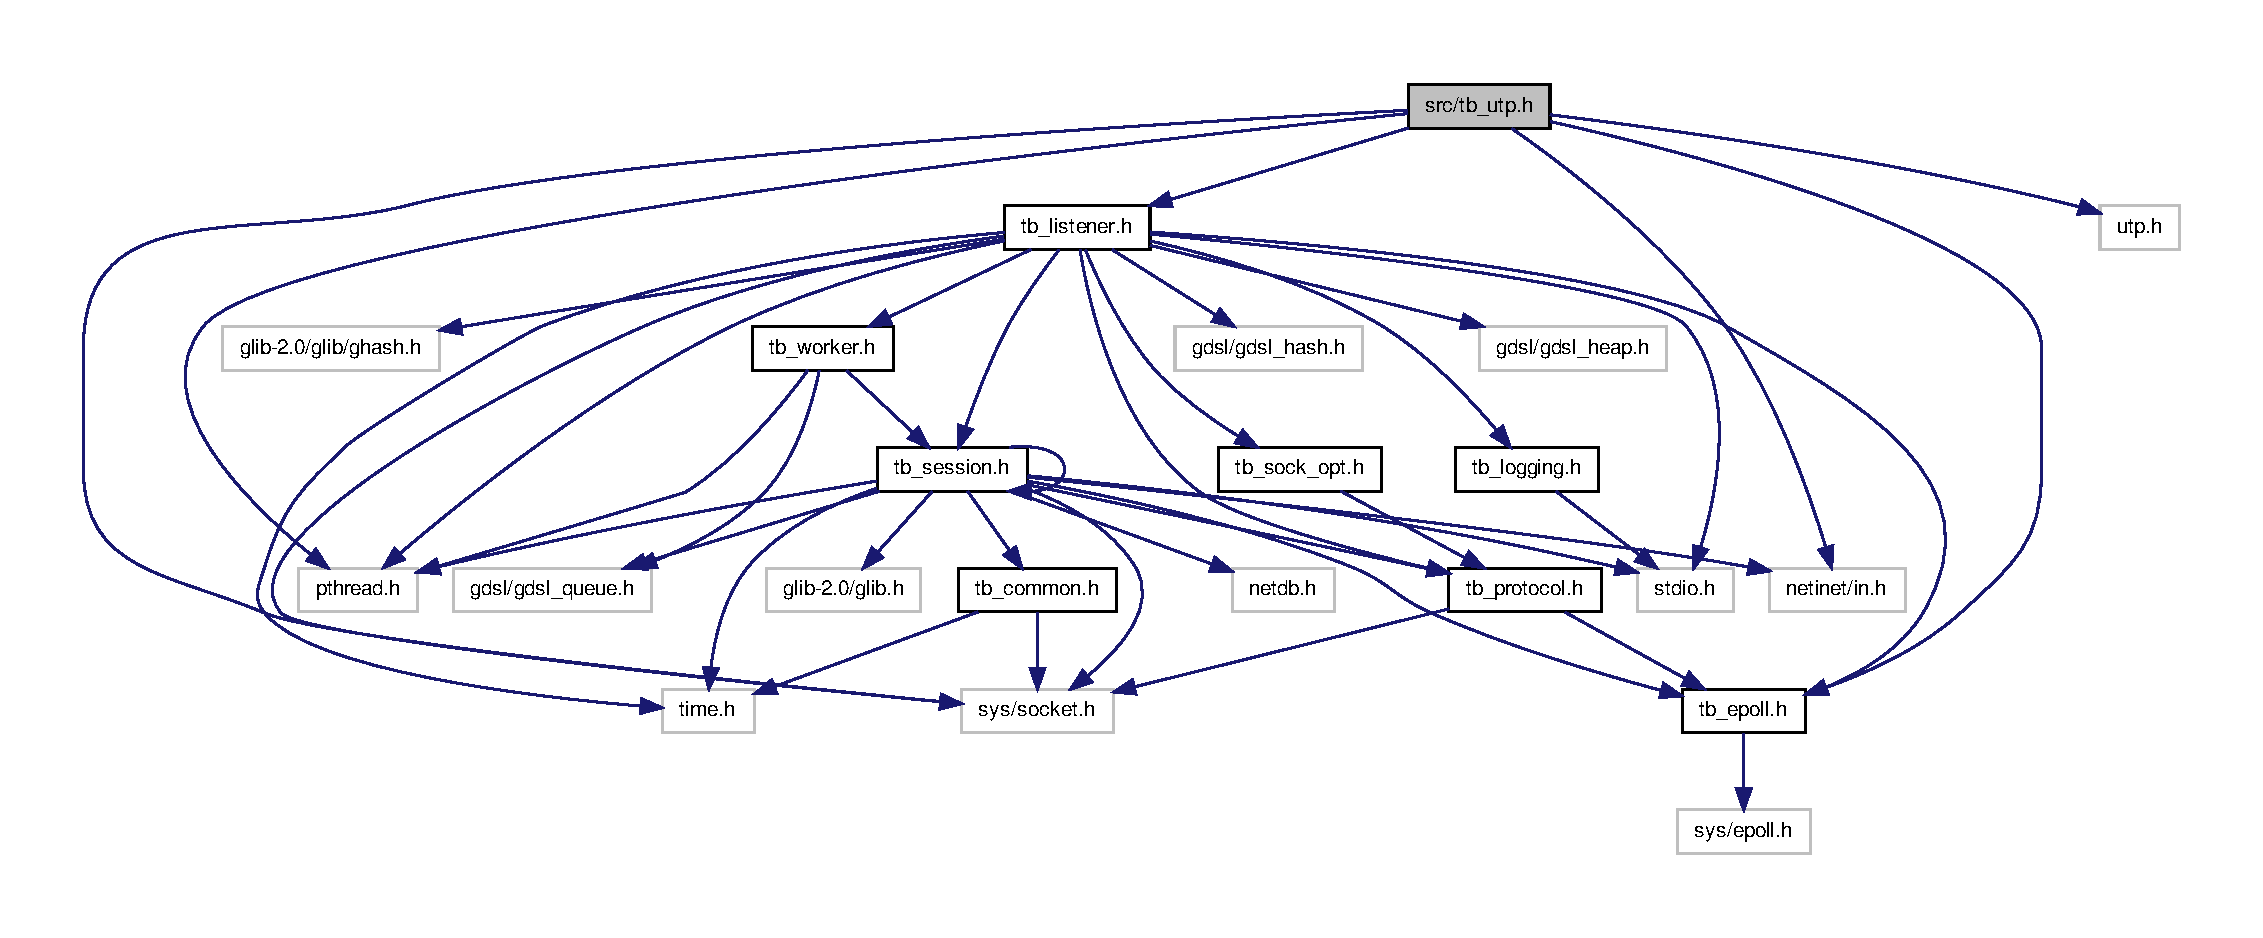
\includegraphics[width=350pt]{tb__utp_8h__incl}
\end{center}
\end{figure}
This graph shows which files directly or indirectly include this file\-:\nopagebreak
\begin{figure}[H]
\begin{center}
\leavevmode
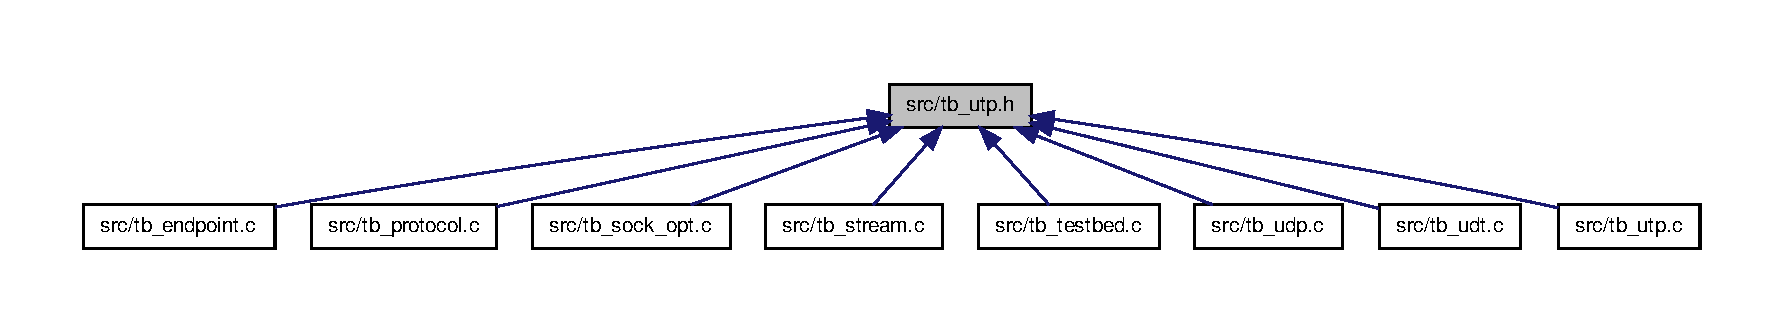
\includegraphics[width=350pt]{tb__utp_8h__dep__incl}
\end{center}
\end{figure}
\subsection*{Data Structures}
\begin{DoxyCompactItemize}
\item 
struct \hyperlink{structtb__utp__t}{tb\-\_\-utp\-\_\-t}
\end{DoxyCompactItemize}
\subsection*{Enumerations}
\begin{DoxyCompactItemize}
\item 
enum \hyperlink{tb__utp_8h_a54540058c7bc0132aaca1effda0191ac}{tb\-\_\-utp\-\_\-state} \{ \hyperlink{tb__utp_8h_a54540058c7bc0132aaca1effda0191aca90d44cdf88d6ec78d67a2dd45d20f206}{U\-T\-P\-\_\-\-S\-T\-A\-T\-E\-\_\-\-C\-R\-E\-A\-T\-E\-D} =  0, 
\hyperlink{tb__utp_8h_a54540058c7bc0132aaca1effda0191aca1e923f48404e9e144620c8d8c8cfc83d}{U\-T\-P\-\_\-\-S\-T\-A\-T\-E\-\_\-\-E\-R\-R\-O\-R} =  5
 \}
\end{DoxyCompactItemize}
\subsection*{Functions}
\begin{DoxyCompactItemize}
\item 
\hyperlink{structtb__utp__t}{tb\-\_\-utp\-\_\-t} $\ast$ \hyperlink{tb__utp_8h_a506a49d3c557eba2fef9b778738743b6}{tb\-\_\-utp\-\_\-setup} ()
\item 
int \hyperlink{tb__utp_8h_a24564db4f7608a8476e4a0138730c7eb}{tb\-\_\-utp\-\_\-get\-\_\-state} () \-\_\-\-\_\-attribute\-\_\-\-\_\-((always\-\_\-inline))
\item 
int \hyperlink{tb__utp_8h_ab7c3fb612ca38a7954c68aec1b4c9d0f}{tb\-\_\-utp\-\_\-set\-\_\-buffers} (size\-\_\-t send\-\_\-buf, size\-\_\-t recv\-\_\-buf)
\item 
void \hyperlink{tb__utp_8h_a26220ca07feac95d0ebdccfaf0228f86}{tb\-\_\-utp\-\_\-read} (void $\ast$userdata, const byte $\ast$bytes, size\-\_\-t count)
\item 
void \hyperlink{tb__utp_8h_a435677dbfa73e419e5155d978ee893c4}{tb\-\_\-utp\-\_\-write} (void $\ast$userdata, byte $\ast$bytes, size\-\_\-t count)
\item 
size\-\_\-t \hyperlink{tb__utp_8h_a78dc4e9a5c6efe713d6bac1e968ce6f1}{tb\-\_\-utp\-\_\-get\-\_\-\-Rcv\-\_\-buff} (void $\ast$userdata)
\item 
void \hyperlink{tb__utp_8h_a1e25222015d067d9bfdf2046b27b58af}{tb\-\_\-utp\-\_\-state\-\_\-change} (void $\ast$userdata, int state)
\item 
void \hyperlink{tb__utp_8h_ab15274bd142f9d742f43ff8670eee3cd}{tb\-\_\-utp\-\_\-error} (void $\ast$userdata, int errcode)
\item 
void \hyperlink{tb__utp_8h_af31fb5ebecca7ed41d3b82654a6d57c6}{tb\-\_\-utp\-\_\-overhead} (void $\ast$userdata, int send, size\-\_\-t count, int type)
\item 
void \hyperlink{tb__utp_8h_a11b6cdd962696b52f2fcac93df1e28e3}{tb\-\_\-utp\-\_\-send\-\_\-to} (void $\ast$userdata, const byte $\ast$p, size\-\_\-t len, const struct sockaddr $\ast$to, socklen\-\_\-t tolen)
\item 
void \hyperlink{tb__utp_8h_a43444f296566ed304ac2934328dd20a0}{tb\-\_\-utp\-\_\-incoming} (void $\ast$userdata, struct U\-T\-P\-Socket $\ast$socket)
\begin{DoxyCompactList}\small\item\em callback, for incoming connections. \end{DoxyCompactList}\item 
int \hyperlink{tb__utp_8h_a041f0d563dc3f8f49012bc7d73f04e2a}{tb\-\_\-utp\-\_\-setsockopt} (int opt, int val)
\begin{DoxyCompactList}\small\item\em Set the given option on a utp socket. \end{DoxyCompactList}\item 
int \hyperlink{tb__utp_8h_a07325129f2f67a976ddd914e71b67881}{tb\-\_\-utp\-\_\-socket} (\hyperlink{structtb__utp__t}{tb\-\_\-utp\-\_\-t} $\ast$utp, int domain, int socktype, int protocol)
\item 
int \hyperlink{tb__utp_8h_ae499f3155494fdc2ea5e53375c1ab5ed}{tb\-\_\-utp\-\_\-connect} (\hyperlink{structtb__utp__t}{tb\-\_\-utp\-\_\-t} $\ast$utp, const struct sockaddr $\ast$addr, socklen\-\_\-t len)
\item 
int \hyperlink{tb__utp_8h_a9dca05324926fb62deab6aa46f130696}{tb\-\_\-utp\-\_\-send} (\hyperlink{structtb__utp__t}{tb\-\_\-utp\-\_\-t} $\ast$utp, void $\ast$buf, size\-\_\-t n)
\item 
int \hyperlink{tb__utp_8h_a0a3ee276e6b51794bee3e7d3867d6051}{tb\-\_\-utp\-\_\-recv\-\_\-data} ()
\item 
int \hyperlink{tb__utp_8h_a5d7b36bb591c90e72dfcadf19ac5152e}{tb\-\_\-utp\-\_\-recv\-\_\-from} (int fd, void $\ast$buf, size\-\_\-t n, unsigned int flags, const struct sockaddr $\ast$to, socklen\-\_\-t $\ast$tolen)
\item 
int \hyperlink{tb__utp_8h_a166ed93b320918ba496852d8e4b37059}{tb\-\_\-utp\-\_\-event} (int events, void $\ast$data)
\begin{DoxyCompactList}\small\item\em Callback used by epoll events. \end{DoxyCompactList}\item 
int \hyperlink{tb__utp_8h_a73863f08a2e18eb80fac12509f0ccaff}{tb\-\_\-utp\-\_\-recv} (\hyperlink{structtb__utp__t}{tb\-\_\-utp\-\_\-t} $\ast$utp, char $\ast$buff, int size)
\begin{DoxyCompactList}\small\item\em Receive data from a u\-T\-P socket. \end{DoxyCompactList}\item 
int \hyperlink{tb__utp_8h_a00c956cd2abf69fde14be69ff5e7aa0c}{tb\-\_\-utp\-\_\-funct\-\_\-exit} ()
\item 
int \hyperlink{tb__utp_8h_ab3bd87fbc20dbbd52543b2fab384f29f}{tb\-\_\-utp\-\_\-error\-\_\-handle} (int value, int err\-\_\-no)
\item 
int \hyperlink{tb__utp_8h_a914e27dc988c6efc694ad951dadefc6b}{tb\-\_\-utp\-\_\-close} (\hyperlink{structtb__utp__t}{tb\-\_\-utp\-\_\-t} $\ast$utp)
\item 
int \hyperlink{tb__utp_8h_aaef934c0644a4ded7635420534b2bd01}{tb\-\_\-utp\-\_\-client} (\hyperlink{structtb__listener__t}{tb\-\_\-listener\-\_\-t} $\ast$listener)
\begin{DoxyCompactList}\small\item\em Upload using the u\-T\-P protocol. \end{DoxyCompactList}\item 
int \hyperlink{tb__utp_8h_aacb2150e3f5d787a6d04e4c69663f643}{tb\-\_\-utp\-\_\-m\-\_\-server} (\hyperlink{structtb__listener__t}{tb\-\_\-listener\-\_\-t} $\ast$listener)
\begin{DoxyCompactList}\small\item\em Create a multiconnection server using u\-T\-P. \end{DoxyCompactList}\item 
int \hyperlink{tb__utp_8h_a91f1cecaee23c1889b8588111d17ddb1}{tb\-\_\-utp\-\_\-m\-\_\-event} (int events, void $\ast$data)
\begin{DoxyCompactList}\small\item\em Event called by epoll. \end{DoxyCompactList}\item 
void \hyperlink{tb__utp_8h_a7fe7f3ac875ad5df2f011c70db45f644}{tb\-\_\-utp\-\_\-m\-\_\-new\-\_\-conn} (void $\ast$userdata, struct U\-T\-P\-Socket $\ast$socket)
\begin{DoxyCompactList}\small\item\em Called when creating a new connection. \end{DoxyCompactList}\item 
int \hyperlink{tb__utp_8h_a4701d9551ad1e0d73019590b729b6224}{tb\-\_\-utp\-\_\-server} (\hyperlink{structtb__listener__t}{tb\-\_\-listener\-\_\-t} $\ast$listener)
\begin{DoxyCompactList}\small\item\em Run a server with u\-T\-P. \end{DoxyCompactList}\end{DoxyCompactItemize}


\subsection{Enumeration Type Documentation}
\hypertarget{tb__utp_8h_a54540058c7bc0132aaca1effda0191ac}{\index{tb\-\_\-utp.\-h@{tb\-\_\-utp.\-h}!tb\-\_\-utp\-\_\-state@{tb\-\_\-utp\-\_\-state}}
\index{tb\-\_\-utp\-\_\-state@{tb\-\_\-utp\-\_\-state}!tb_utp.h@{tb\-\_\-utp.\-h}}
\subsubsection[{tb\-\_\-utp\-\_\-state}]{\setlength{\rightskip}{0pt plus 5cm}enum {\bf tb\-\_\-utp\-\_\-state}}}\label{tb__utp_8h_a54540058c7bc0132aaca1effda0191ac}
\begin{Desc}
\item[Enumerator\-: ]\par
\begin{description}
\index{U\-T\-P\-\_\-\-S\-T\-A\-T\-E\-\_\-\-C\-R\-E\-A\-T\-E\-D@{U\-T\-P\-\_\-\-S\-T\-A\-T\-E\-\_\-\-C\-R\-E\-A\-T\-E\-D}!tb\-\_\-utp.\-h@{tb\-\_\-utp.\-h}}\index{tb\-\_\-utp.\-h@{tb\-\_\-utp.\-h}!U\-T\-P\-\_\-\-S\-T\-A\-T\-E\-\_\-\-C\-R\-E\-A\-T\-E\-D@{U\-T\-P\-\_\-\-S\-T\-A\-T\-E\-\_\-\-C\-R\-E\-A\-T\-E\-D}}\item[{\em 
\hypertarget{tb__utp_8h_a54540058c7bc0132aaca1effda0191aca90d44cdf88d6ec78d67a2dd45d20f206}{U\-T\-P\-\_\-\-S\-T\-A\-T\-E\-\_\-\-C\-R\-E\-A\-T\-E\-D}\label{tb__utp_8h_a54540058c7bc0132aaca1effda0191aca90d44cdf88d6ec78d67a2dd45d20f206}
}]\index{U\-T\-P\-\_\-\-S\-T\-A\-T\-E\-\_\-\-E\-R\-R\-O\-R@{U\-T\-P\-\_\-\-S\-T\-A\-T\-E\-\_\-\-E\-R\-R\-O\-R}!tb\-\_\-utp.\-h@{tb\-\_\-utp.\-h}}\index{tb\-\_\-utp.\-h@{tb\-\_\-utp.\-h}!U\-T\-P\-\_\-\-S\-T\-A\-T\-E\-\_\-\-E\-R\-R\-O\-R@{U\-T\-P\-\_\-\-S\-T\-A\-T\-E\-\_\-\-E\-R\-R\-O\-R}}\item[{\em 
\hypertarget{tb__utp_8h_a54540058c7bc0132aaca1effda0191aca1e923f48404e9e144620c8d8c8cfc83d}{U\-T\-P\-\_\-\-S\-T\-A\-T\-E\-\_\-\-E\-R\-R\-O\-R}\label{tb__utp_8h_a54540058c7bc0132aaca1effda0191aca1e923f48404e9e144620c8d8c8cfc83d}
}]\end{description}
\end{Desc}



Definition at line 59 of file tb\-\_\-utp.\-h.



\subsection{Function Documentation}
\hypertarget{tb__utp_8h_aaef934c0644a4ded7635420534b2bd01}{\index{tb\-\_\-utp.\-h@{tb\-\_\-utp.\-h}!tb\-\_\-utp\-\_\-client@{tb\-\_\-utp\-\_\-client}}
\index{tb\-\_\-utp\-\_\-client@{tb\-\_\-utp\-\_\-client}!tb_utp.h@{tb\-\_\-utp.\-h}}
\subsubsection[{tb\-\_\-utp\-\_\-client}]{\setlength{\rightskip}{0pt plus 5cm}int tb\-\_\-utp\-\_\-client (
\begin{DoxyParamCaption}
\item[{{\bf tb\-\_\-listener\-\_\-t} $\ast$}]{listener}
\end{DoxyParamCaption}
)}}\label{tb__utp_8h_aaef934c0644a4ded7635420534b2bd01}


Upload using the u\-T\-P protocol. 

Upload data using the u\-T\-P protocol. 

Definition at line 340 of file tb\-\_\-utp.\-c.

\hypertarget{tb__utp_8h_a914e27dc988c6efc694ad951dadefc6b}{\index{tb\-\_\-utp.\-h@{tb\-\_\-utp.\-h}!tb\-\_\-utp\-\_\-close@{tb\-\_\-utp\-\_\-close}}
\index{tb\-\_\-utp\-\_\-close@{tb\-\_\-utp\-\_\-close}!tb_utp.h@{tb\-\_\-utp.\-h}}
\subsubsection[{tb\-\_\-utp\-\_\-close}]{\setlength{\rightskip}{0pt plus 5cm}int tb\-\_\-utp\-\_\-close (
\begin{DoxyParamCaption}
\item[{{\bf tb\-\_\-utp\-\_\-t} $\ast$}]{utp}
\end{DoxyParamCaption}
)}}\label{tb__utp_8h_a914e27dc988c6efc694ad951dadefc6b}


Definition at line 308 of file tb\-\_\-utp.\-c.

\hypertarget{tb__utp_8h_ae499f3155494fdc2ea5e53375c1ab5ed}{\index{tb\-\_\-utp.\-h@{tb\-\_\-utp.\-h}!tb\-\_\-utp\-\_\-connect@{tb\-\_\-utp\-\_\-connect}}
\index{tb\-\_\-utp\-\_\-connect@{tb\-\_\-utp\-\_\-connect}!tb_utp.h@{tb\-\_\-utp.\-h}}
\subsubsection[{tb\-\_\-utp\-\_\-connect}]{\setlength{\rightskip}{0pt plus 5cm}int tb\-\_\-utp\-\_\-connect (
\begin{DoxyParamCaption}
\item[{{\bf tb\-\_\-utp\-\_\-t} $\ast$}]{utp, }
\item[{const struct sockaddr $\ast$}]{addr, }
\item[{socklen\-\_\-t}]{len}
\end{DoxyParamCaption}
)}}\label{tb__utp_8h_ae499f3155494fdc2ea5e53375c1ab5ed}


Definition at line 187 of file tb\-\_\-utp.\-c.

\hypertarget{tb__utp_8h_ab15274bd142f9d742f43ff8670eee3cd}{\index{tb\-\_\-utp.\-h@{tb\-\_\-utp.\-h}!tb\-\_\-utp\-\_\-error@{tb\-\_\-utp\-\_\-error}}
\index{tb\-\_\-utp\-\_\-error@{tb\-\_\-utp\-\_\-error}!tb_utp.h@{tb\-\_\-utp.\-h}}
\subsubsection[{tb\-\_\-utp\-\_\-error}]{\setlength{\rightskip}{0pt plus 5cm}void tb\-\_\-utp\-\_\-error (
\begin{DoxyParamCaption}
\item[{void $\ast$}]{userdata, }
\item[{int}]{errcode}
\end{DoxyParamCaption}
)}}\label{tb__utp_8h_ab15274bd142f9d742f43ff8670eee3cd}


Definition at line 121 of file tb\-\_\-utp.\-c.

\hypertarget{tb__utp_8h_ab3bd87fbc20dbbd52543b2fab384f29f}{\index{tb\-\_\-utp.\-h@{tb\-\_\-utp.\-h}!tb\-\_\-utp\-\_\-error\-\_\-handle@{tb\-\_\-utp\-\_\-error\-\_\-handle}}
\index{tb\-\_\-utp\-\_\-error\-\_\-handle@{tb\-\_\-utp\-\_\-error\-\_\-handle}!tb_utp.h@{tb\-\_\-utp.\-h}}
\subsubsection[{tb\-\_\-utp\-\_\-error\-\_\-handle}]{\setlength{\rightskip}{0pt plus 5cm}int tb\-\_\-utp\-\_\-error\-\_\-handle (
\begin{DoxyParamCaption}
\item[{int}]{value, }
\item[{int}]{err\-\_\-no}
\end{DoxyParamCaption}
)}}\label{tb__utp_8h_ab3bd87fbc20dbbd52543b2fab384f29f}


Definition at line 302 of file tb\-\_\-utp.\-c.

\hypertarget{tb__utp_8h_a166ed93b320918ba496852d8e4b37059}{\index{tb\-\_\-utp.\-h@{tb\-\_\-utp.\-h}!tb\-\_\-utp\-\_\-event@{tb\-\_\-utp\-\_\-event}}
\index{tb\-\_\-utp\-\_\-event@{tb\-\_\-utp\-\_\-event}!tb_utp.h@{tb\-\_\-utp.\-h}}
\subsubsection[{tb\-\_\-utp\-\_\-event}]{\setlength{\rightskip}{0pt plus 5cm}int tb\-\_\-utp\-\_\-event (
\begin{DoxyParamCaption}
\item[{int}]{events, }
\item[{void $\ast$}]{data}
\end{DoxyParamCaption}
)}}\label{tb__utp_8h_a166ed93b320918ba496852d8e4b37059}


Callback used by epoll events. 



Definition at line 239 of file tb\-\_\-utp.\-c.

\hypertarget{tb__utp_8h_a00c956cd2abf69fde14be69ff5e7aa0c}{\index{tb\-\_\-utp.\-h@{tb\-\_\-utp.\-h}!tb\-\_\-utp\-\_\-funct\-\_\-exit@{tb\-\_\-utp\-\_\-funct\-\_\-exit}}
\index{tb\-\_\-utp\-\_\-funct\-\_\-exit@{tb\-\_\-utp\-\_\-funct\-\_\-exit}!tb_utp.h@{tb\-\_\-utp.\-h}}
\subsubsection[{tb\-\_\-utp\-\_\-funct\-\_\-exit}]{\setlength{\rightskip}{0pt plus 5cm}int tb\-\_\-utp\-\_\-funct\-\_\-exit (
\begin{DoxyParamCaption}
{}
\end{DoxyParamCaption}
)}}\label{tb__utp_8h_a00c956cd2abf69fde14be69ff5e7aa0c}


Definition at line 296 of file tb\-\_\-utp.\-c.

\hypertarget{tb__utp_8h_a78dc4e9a5c6efe713d6bac1e968ce6f1}{\index{tb\-\_\-utp.\-h@{tb\-\_\-utp.\-h}!tb\-\_\-utp\-\_\-get\-\_\-\-Rcv\-\_\-buff@{tb\-\_\-utp\-\_\-get\-\_\-\-Rcv\-\_\-buff}}
\index{tb\-\_\-utp\-\_\-get\-\_\-\-Rcv\-\_\-buff@{tb\-\_\-utp\-\_\-get\-\_\-\-Rcv\-\_\-buff}!tb_utp.h@{tb\-\_\-utp.\-h}}
\subsubsection[{tb\-\_\-utp\-\_\-get\-\_\-\-Rcv\-\_\-buff}]{\setlength{\rightskip}{0pt plus 5cm}size\-\_\-t tb\-\_\-utp\-\_\-get\-\_\-\-Rcv\-\_\-buff (
\begin{DoxyParamCaption}
\item[{void $\ast$}]{userdata}
\end{DoxyParamCaption}
)}}\label{tb__utp_8h_a78dc4e9a5c6efe713d6bac1e968ce6f1}


Definition at line 92 of file tb\-\_\-utp.\-c.

\hypertarget{tb__utp_8h_a24564db4f7608a8476e4a0138730c7eb}{\index{tb\-\_\-utp.\-h@{tb\-\_\-utp.\-h}!tb\-\_\-utp\-\_\-get\-\_\-state@{tb\-\_\-utp\-\_\-get\-\_\-state}}
\index{tb\-\_\-utp\-\_\-get\-\_\-state@{tb\-\_\-utp\-\_\-get\-\_\-state}!tb_utp.h@{tb\-\_\-utp.\-h}}
\subsubsection[{tb\-\_\-utp\-\_\-get\-\_\-state}]{\setlength{\rightskip}{0pt plus 5cm}int tb\-\_\-utp\-\_\-get\-\_\-state (
\begin{DoxyParamCaption}
{}
\end{DoxyParamCaption}
)\hspace{0.3cm}{\ttfamily [inline]}}}\label{tb__utp_8h_a24564db4f7608a8476e4a0138730c7eb}
\hypertarget{tb__utp_8h_a43444f296566ed304ac2934328dd20a0}{\index{tb\-\_\-utp.\-h@{tb\-\_\-utp.\-h}!tb\-\_\-utp\-\_\-incoming@{tb\-\_\-utp\-\_\-incoming}}
\index{tb\-\_\-utp\-\_\-incoming@{tb\-\_\-utp\-\_\-incoming}!tb_utp.h@{tb\-\_\-utp.\-h}}
\subsubsection[{tb\-\_\-utp\-\_\-incoming}]{\setlength{\rightskip}{0pt plus 5cm}void tb\-\_\-utp\-\_\-incoming (
\begin{DoxyParamCaption}
\item[{void $\ast$}]{userdata, }
\item[{struct U\-T\-P\-Socket $\ast$}]{socket}
\end{DoxyParamCaption}
)}}\label{tb__utp_8h_a43444f296566ed304ac2934328dd20a0}


callback, for incoming connections. 

Called by the u\-T\-P library when incoming data is deemed to be data for a new connection. 

Definition at line 153 of file tb\-\_\-utp.\-c.

\hypertarget{tb__utp_8h_a91f1cecaee23c1889b8588111d17ddb1}{\index{tb\-\_\-utp.\-h@{tb\-\_\-utp.\-h}!tb\-\_\-utp\-\_\-m\-\_\-event@{tb\-\_\-utp\-\_\-m\-\_\-event}}
\index{tb\-\_\-utp\-\_\-m\-\_\-event@{tb\-\_\-utp\-\_\-m\-\_\-event}!tb_utp.h@{tb\-\_\-utp.\-h}}
\subsubsection[{tb\-\_\-utp\-\_\-m\-\_\-event}]{\setlength{\rightskip}{0pt plus 5cm}int tb\-\_\-utp\-\_\-m\-\_\-event (
\begin{DoxyParamCaption}
\item[{int}]{events, }
\item[{void $\ast$}]{data}
\end{DoxyParamCaption}
)}}\label{tb__utp_8h_a91f1cecaee23c1889b8588111d17ddb1}


Event called by epoll. 



Definition at line 428 of file tb\-\_\-utp.\-c.

\hypertarget{tb__utp_8h_a7fe7f3ac875ad5df2f011c70db45f644}{\index{tb\-\_\-utp.\-h@{tb\-\_\-utp.\-h}!tb\-\_\-utp\-\_\-m\-\_\-new\-\_\-conn@{tb\-\_\-utp\-\_\-m\-\_\-new\-\_\-conn}}
\index{tb\-\_\-utp\-\_\-m\-\_\-new\-\_\-conn@{tb\-\_\-utp\-\_\-m\-\_\-new\-\_\-conn}!tb_utp.h@{tb\-\_\-utp.\-h}}
\subsubsection[{tb\-\_\-utp\-\_\-m\-\_\-new\-\_\-conn}]{\setlength{\rightskip}{0pt plus 5cm}void tb\-\_\-utp\-\_\-m\-\_\-new\-\_\-conn (
\begin{DoxyParamCaption}
\item[{void $\ast$}]{userdata, }
\item[{struct U\-T\-P\-Socket $\ast$}]{socket}
\end{DoxyParamCaption}
)}}\label{tb__utp_8h_a7fe7f3ac875ad5df2f011c70db45f644}


Called when creating a new connection. 



Definition at line 469 of file tb\-\_\-utp.\-c.

\hypertarget{tb__utp_8h_aacb2150e3f5d787a6d04e4c69663f643}{\index{tb\-\_\-utp.\-h@{tb\-\_\-utp.\-h}!tb\-\_\-utp\-\_\-m\-\_\-server@{tb\-\_\-utp\-\_\-m\-\_\-server}}
\index{tb\-\_\-utp\-\_\-m\-\_\-server@{tb\-\_\-utp\-\_\-m\-\_\-server}!tb_utp.h@{tb\-\_\-utp.\-h}}
\subsubsection[{tb\-\_\-utp\-\_\-m\-\_\-server}]{\setlength{\rightskip}{0pt plus 5cm}int tb\-\_\-utp\-\_\-m\-\_\-server (
\begin{DoxyParamCaption}
\item[{{\bf tb\-\_\-listener\-\_\-t} $\ast$}]{listener}
\end{DoxyParamCaption}
)}}\label{tb__utp_8h_aacb2150e3f5d787a6d04e4c69663f643}


Create a multiconnection server using u\-T\-P. 



Definition at line 421 of file tb\-\_\-utp.\-c.

\hypertarget{tb__utp_8h_af31fb5ebecca7ed41d3b82654a6d57c6}{\index{tb\-\_\-utp.\-h@{tb\-\_\-utp.\-h}!tb\-\_\-utp\-\_\-overhead@{tb\-\_\-utp\-\_\-overhead}}
\index{tb\-\_\-utp\-\_\-overhead@{tb\-\_\-utp\-\_\-overhead}!tb_utp.h@{tb\-\_\-utp.\-h}}
\subsubsection[{tb\-\_\-utp\-\_\-overhead}]{\setlength{\rightskip}{0pt plus 5cm}void tb\-\_\-utp\-\_\-overhead (
\begin{DoxyParamCaption}
\item[{void $\ast$}]{userdata, }
\item[{int}]{send, }
\item[{size\-\_\-t}]{count, }
\item[{int}]{type}
\end{DoxyParamCaption}
)}}\label{tb__utp_8h_af31fb5ebecca7ed41d3b82654a6d57c6}


Definition at line 133 of file tb\-\_\-utp.\-c.

\hypertarget{tb__utp_8h_a26220ca07feac95d0ebdccfaf0228f86}{\index{tb\-\_\-utp.\-h@{tb\-\_\-utp.\-h}!tb\-\_\-utp\-\_\-read@{tb\-\_\-utp\-\_\-read}}
\index{tb\-\_\-utp\-\_\-read@{tb\-\_\-utp\-\_\-read}!tb_utp.h@{tb\-\_\-utp.\-h}}
\subsubsection[{tb\-\_\-utp\-\_\-read}]{\setlength{\rightskip}{0pt plus 5cm}void tb\-\_\-utp\-\_\-read (
\begin{DoxyParamCaption}
\item[{void $\ast$}]{userdata, }
\item[{const byte $\ast$}]{bytes, }
\item[{size\-\_\-t}]{count}
\end{DoxyParamCaption}
)}}\label{tb__utp_8h_a26220ca07feac95d0ebdccfaf0228f86}


Definition at line 74 of file tb\-\_\-utp.\-c.

\hypertarget{tb__utp_8h_a73863f08a2e18eb80fac12509f0ccaff}{\index{tb\-\_\-utp.\-h@{tb\-\_\-utp.\-h}!tb\-\_\-utp\-\_\-recv@{tb\-\_\-utp\-\_\-recv}}
\index{tb\-\_\-utp\-\_\-recv@{tb\-\_\-utp\-\_\-recv}!tb_utp.h@{tb\-\_\-utp.\-h}}
\subsubsection[{tb\-\_\-utp\-\_\-recv}]{\setlength{\rightskip}{0pt plus 5cm}int tb\-\_\-utp\-\_\-recv (
\begin{DoxyParamCaption}
\item[{{\bf tb\-\_\-utp\-\_\-t} $\ast$}]{utp, }
\item[{char $\ast$}]{buff, }
\item[{int}]{size}
\end{DoxyParamCaption}
)}}\label{tb__utp_8h_a73863f08a2e18eb80fac12509f0ccaff}


Receive data from a u\-T\-P socket. 



Definition at line 286 of file tb\-\_\-utp.\-c.

\hypertarget{tb__utp_8h_a0a3ee276e6b51794bee3e7d3867d6051}{\index{tb\-\_\-utp.\-h@{tb\-\_\-utp.\-h}!tb\-\_\-utp\-\_\-recv\-\_\-data@{tb\-\_\-utp\-\_\-recv\-\_\-data}}
\index{tb\-\_\-utp\-\_\-recv\-\_\-data@{tb\-\_\-utp\-\_\-recv\-\_\-data}!tb_utp.h@{tb\-\_\-utp.\-h}}
\subsubsection[{tb\-\_\-utp\-\_\-recv\-\_\-data}]{\setlength{\rightskip}{0pt plus 5cm}int tb\-\_\-utp\-\_\-recv\-\_\-data (
\begin{DoxyParamCaption}
{}
\end{DoxyParamCaption}
)}}\label{tb__utp_8h_a0a3ee276e6b51794bee3e7d3867d6051}
\hypertarget{tb__utp_8h_a5d7b36bb591c90e72dfcadf19ac5152e}{\index{tb\-\_\-utp.\-h@{tb\-\_\-utp.\-h}!tb\-\_\-utp\-\_\-recv\-\_\-from@{tb\-\_\-utp\-\_\-recv\-\_\-from}}
\index{tb\-\_\-utp\-\_\-recv\-\_\-from@{tb\-\_\-utp\-\_\-recv\-\_\-from}!tb_utp.h@{tb\-\_\-utp.\-h}}
\subsubsection[{tb\-\_\-utp\-\_\-recv\-\_\-from}]{\setlength{\rightskip}{0pt plus 5cm}int tb\-\_\-utp\-\_\-recv\-\_\-from (
\begin{DoxyParamCaption}
\item[{int}]{fd, }
\item[{void $\ast$}]{buf, }
\item[{size\-\_\-t}]{n, }
\item[{unsigned int}]{flags, }
\item[{const struct sockaddr $\ast$}]{to, }
\item[{socklen\-\_\-t $\ast$}]{tolen}
\end{DoxyParamCaption}
)}}\label{tb__utp_8h_a5d7b36bb591c90e72dfcadf19ac5152e}
\hypertarget{tb__utp_8h_a9dca05324926fb62deab6aa46f130696}{\index{tb\-\_\-utp.\-h@{tb\-\_\-utp.\-h}!tb\-\_\-utp\-\_\-send@{tb\-\_\-utp\-\_\-send}}
\index{tb\-\_\-utp\-\_\-send@{tb\-\_\-utp\-\_\-send}!tb_utp.h@{tb\-\_\-utp.\-h}}
\subsubsection[{tb\-\_\-utp\-\_\-send}]{\setlength{\rightskip}{0pt plus 5cm}int tb\-\_\-utp\-\_\-send (
\begin{DoxyParamCaption}
\item[{{\bf tb\-\_\-utp\-\_\-t} $\ast$}]{utp, }
\item[{void $\ast$}]{buf, }
\item[{size\-\_\-t}]{n}
\end{DoxyParamCaption}
)}}\label{tb__utp_8h_a9dca05324926fb62deab6aa46f130696}


Definition at line 206 of file tb\-\_\-utp.\-c.

\hypertarget{tb__utp_8h_a11b6cdd962696b52f2fcac93df1e28e3}{\index{tb\-\_\-utp.\-h@{tb\-\_\-utp.\-h}!tb\-\_\-utp\-\_\-send\-\_\-to@{tb\-\_\-utp\-\_\-send\-\_\-to}}
\index{tb\-\_\-utp\-\_\-send\-\_\-to@{tb\-\_\-utp\-\_\-send\-\_\-to}!tb_utp.h@{tb\-\_\-utp.\-h}}
\subsubsection[{tb\-\_\-utp\-\_\-send\-\_\-to}]{\setlength{\rightskip}{0pt plus 5cm}void tb\-\_\-utp\-\_\-send\-\_\-to (
\begin{DoxyParamCaption}
\item[{void $\ast$}]{userdata, }
\item[{const byte $\ast$}]{p, }
\item[{size\-\_\-t}]{len, }
\item[{const struct sockaddr $\ast$}]{to, }
\item[{socklen\-\_\-t}]{tolen}
\end{DoxyParamCaption}
)}}\label{tb__utp_8h_a11b6cdd962696b52f2fcac93df1e28e3}


Definition at line 139 of file tb\-\_\-utp.\-c.

\hypertarget{tb__utp_8h_a4701d9551ad1e0d73019590b729b6224}{\index{tb\-\_\-utp.\-h@{tb\-\_\-utp.\-h}!tb\-\_\-utp\-\_\-server@{tb\-\_\-utp\-\_\-server}}
\index{tb\-\_\-utp\-\_\-server@{tb\-\_\-utp\-\_\-server}!tb_utp.h@{tb\-\_\-utp.\-h}}
\subsubsection[{tb\-\_\-utp\-\_\-server}]{\setlength{\rightskip}{0pt plus 5cm}int tb\-\_\-utp\-\_\-server (
\begin{DoxyParamCaption}
\item[{{\bf tb\-\_\-listener\-\_\-t} $\ast$}]{listener}
\end{DoxyParamCaption}
)}}\label{tb__utp_8h_a4701d9551ad1e0d73019590b729b6224}


Run a server with u\-T\-P. 



Definition at line 475 of file tb\-\_\-utp.\-c.

\hypertarget{tb__utp_8h_ab7c3fb612ca38a7954c68aec1b4c9d0f}{\index{tb\-\_\-utp.\-h@{tb\-\_\-utp.\-h}!tb\-\_\-utp\-\_\-set\-\_\-buffers@{tb\-\_\-utp\-\_\-set\-\_\-buffers}}
\index{tb\-\_\-utp\-\_\-set\-\_\-buffers@{tb\-\_\-utp\-\_\-set\-\_\-buffers}!tb_utp.h@{tb\-\_\-utp.\-h}}
\subsubsection[{tb\-\_\-utp\-\_\-set\-\_\-buffers}]{\setlength{\rightskip}{0pt plus 5cm}int tb\-\_\-utp\-\_\-set\-\_\-buffers (
\begin{DoxyParamCaption}
\item[{size\-\_\-t}]{send\-\_\-buf, }
\item[{size\-\_\-t}]{recv\-\_\-buf}
\end{DoxyParamCaption}
)}}\label{tb__utp_8h_ab7c3fb612ca38a7954c68aec1b4c9d0f}
\hypertarget{tb__utp_8h_a041f0d563dc3f8f49012bc7d73f04e2a}{\index{tb\-\_\-utp.\-h@{tb\-\_\-utp.\-h}!tb\-\_\-utp\-\_\-setsockopt@{tb\-\_\-utp\-\_\-setsockopt}}
\index{tb\-\_\-utp\-\_\-setsockopt@{tb\-\_\-utp\-\_\-setsockopt}!tb_utp.h@{tb\-\_\-utp.\-h}}
\subsubsection[{tb\-\_\-utp\-\_\-setsockopt}]{\setlength{\rightskip}{0pt plus 5cm}int tb\-\_\-utp\-\_\-setsockopt (
\begin{DoxyParamCaption}
\item[{int}]{opt, }
\item[{int}]{val}
\end{DoxyParamCaption}
)}}\label{tb__utp_8h_a041f0d563dc3f8f49012bc7d73f04e2a}


Set the given option on a utp socket. 

Sets the provided value for the given option. Returns 1 on success. \hypertarget{tb__utp_8h_a506a49d3c557eba2fef9b778738743b6}{\index{tb\-\_\-utp.\-h@{tb\-\_\-utp.\-h}!tb\-\_\-utp\-\_\-setup@{tb\-\_\-utp\-\_\-setup}}
\index{tb\-\_\-utp\-\_\-setup@{tb\-\_\-utp\-\_\-setup}!tb_utp.h@{tb\-\_\-utp.\-h}}
\subsubsection[{tb\-\_\-utp\-\_\-setup}]{\setlength{\rightskip}{0pt plus 5cm}{\bf tb\-\_\-utp\-\_\-t}$\ast$ tb\-\_\-utp\-\_\-setup (
\begin{DoxyParamCaption}
{}
\end{DoxyParamCaption}
)}}\label{tb__utp_8h_a506a49d3c557eba2fef9b778738743b6}


Definition at line 34 of file tb\-\_\-utp.\-c.

\hypertarget{tb__utp_8h_a07325129f2f67a976ddd914e71b67881}{\index{tb\-\_\-utp.\-h@{tb\-\_\-utp.\-h}!tb\-\_\-utp\-\_\-socket@{tb\-\_\-utp\-\_\-socket}}
\index{tb\-\_\-utp\-\_\-socket@{tb\-\_\-utp\-\_\-socket}!tb_utp.h@{tb\-\_\-utp.\-h}}
\subsubsection[{tb\-\_\-utp\-\_\-socket}]{\setlength{\rightskip}{0pt plus 5cm}int tb\-\_\-utp\-\_\-socket (
\begin{DoxyParamCaption}
\item[{{\bf tb\-\_\-utp\-\_\-t} $\ast$}]{utp, }
\item[{int}]{domain, }
\item[{int}]{socktype, }
\item[{int}]{protocol}
\end{DoxyParamCaption}
)}}\label{tb__utp_8h_a07325129f2f67a976ddd914e71b67881}


Definition at line 167 of file tb\-\_\-utp.\-c.

\hypertarget{tb__utp_8h_a1e25222015d067d9bfdf2046b27b58af}{\index{tb\-\_\-utp.\-h@{tb\-\_\-utp.\-h}!tb\-\_\-utp\-\_\-state\-\_\-change@{tb\-\_\-utp\-\_\-state\-\_\-change}}
\index{tb\-\_\-utp\-\_\-state\-\_\-change@{tb\-\_\-utp\-\_\-state\-\_\-change}!tb_utp.h@{tb\-\_\-utp.\-h}}
\subsubsection[{tb\-\_\-utp\-\_\-state\-\_\-change}]{\setlength{\rightskip}{0pt plus 5cm}void tb\-\_\-utp\-\_\-state\-\_\-change (
\begin{DoxyParamCaption}
\item[{void $\ast$}]{userdata, }
\item[{int}]{state}
\end{DoxyParamCaption}
)}}\label{tb__utp_8h_a1e25222015d067d9bfdf2046b27b58af}


Definition at line 98 of file tb\-\_\-utp.\-c.

\hypertarget{tb__utp_8h_a435677dbfa73e419e5155d978ee893c4}{\index{tb\-\_\-utp.\-h@{tb\-\_\-utp.\-h}!tb\-\_\-utp\-\_\-write@{tb\-\_\-utp\-\_\-write}}
\index{tb\-\_\-utp\-\_\-write@{tb\-\_\-utp\-\_\-write}!tb_utp.h@{tb\-\_\-utp.\-h}}
\subsubsection[{tb\-\_\-utp\-\_\-write}]{\setlength{\rightskip}{0pt plus 5cm}void tb\-\_\-utp\-\_\-write (
\begin{DoxyParamCaption}
\item[{void $\ast$}]{userdata, }
\item[{byte $\ast$}]{bytes, }
\item[{size\-\_\-t}]{count}
\end{DoxyParamCaption}
)}}\label{tb__utp_8h_a435677dbfa73e419e5155d978ee893c4}


Definition at line 83 of file tb\-\_\-utp.\-c.


\hypertarget{tb__worker_8c}{\section{src/tb\-\_\-worker.c File Reference}
\label{tb__worker_8c}\index{src/tb\-\_\-worker.\-c@{src/tb\-\_\-worker.\-c}}
}
{\ttfamily \#include \char`\"{}tb\-\_\-worker.\-h\char`\"{}}\\*
{\ttfamily \#include \char`\"{}tb\-\_\-session.\-h\char`\"{}}\\*
{\ttfamily \#include $<$gdsl/gdsl\-\_\-queue.\-h$>$}\\*
{\ttfamily \#include $<$stdlib.\-h$>$}\\*
{\ttfamily \#include $<$string.\-h$>$}\\*
{\ttfamily \#include $<$assert.\-h$>$}\\*
{\ttfamily \#include $<$pthread.\-h$>$}\\*
{\ttfamily \#include $<$stdio.\-h$>$}\\*
{\ttfamily \#include $<$sys/socket.\-h$>$}\\*
Include dependency graph for tb\-\_\-worker.\-c\-:\nopagebreak
\begin{figure}[H]
\begin{center}
\leavevmode
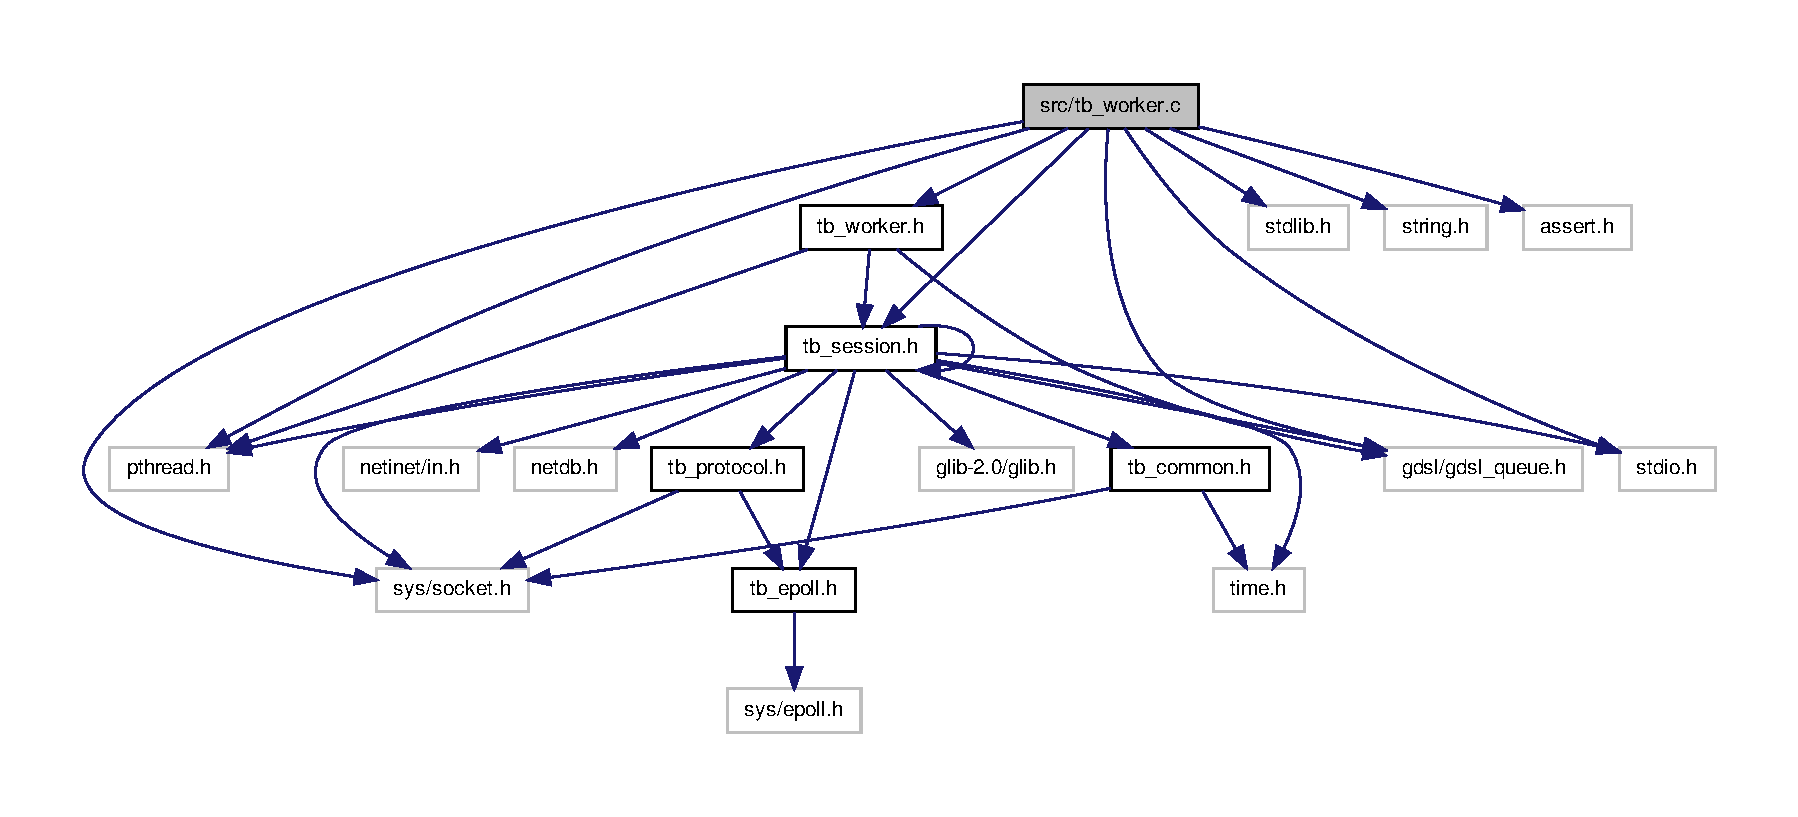
\includegraphics[width=350pt]{tb__worker_8c__incl}
\end{center}
\end{figure}
\subsection*{Functions}
\begin{DoxyCompactItemize}
\item 
void $\ast$ \hyperlink{tb__worker_8c_af9d62097df66ab4d05386c49b45a74e8}{do\-\_\-work} (void $\ast$param)
\begin{DoxyCompactList}\small\item\em Start work. \end{DoxyCompactList}\item 
\hyperlink{structtb__worker__t}{tb\-\_\-worker\-\_\-t} $\ast$ \hyperlink{tb__worker_8c_a10a515d12c8fb7885a5cd5d1a67141fc}{create\-\_\-worker} ()
\begin{DoxyCompactList}\small\item\em Create a new worker, allocating memory as required. \end{DoxyCompactList}\item 
void \hyperlink{tb__worker_8c_aa7815ec198375441b2d6dad28f0c6fce}{destroy\-\_\-worker} (\hyperlink{structtb__worker__t}{tb\-\_\-worker\-\_\-t} $\ast$w)
\begin{DoxyCompactList}\small\item\em Destroy the given worker, freeing memory. \end{DoxyCompactList}\item 
void \hyperlink{tb__worker_8c_aa5ef220c5813db06b41fccbf885a5727}{add\-\_\-work} (\hyperlink{structtb__worker__t}{tb\-\_\-worker\-\_\-t} $\ast$worker, \hyperlink{structtb__session__t}{tb\-\_\-session\-\_\-t} $\ast$data)
\begin{DoxyCompactList}\small\item\em Add work to a worker. \end{DoxyCompactList}\item 
\hyperlink{structtb__session__t}{tb\-\_\-session\-\_\-t} $\ast$ \hyperlink{tb__worker_8c_aceb05b8d10c44e2979cc78b5bde1b369}{get\-\_\-work} (\hyperlink{structtb__worker__t}{tb\-\_\-worker\-\_\-t} $\ast$worker)
\begin{DoxyCompactList}\small\item\em Get work for this worker. \end{DoxyCompactList}\item 
long int \hyperlink{tb__worker_8c_a8746fc48b8ce47ad0bdc8b521f7708d0}{compare\-\_\-workers} (gdsl\-\_\-element\-\_\-t E, void $\ast$value)
\begin{DoxyCompactList}\small\item\em Compare two workers, required by gdsl\-\_\-heap. \end{DoxyCompactList}\end{DoxyCompactItemize}


\subsection{Function Documentation}
\hypertarget{tb__worker_8c_aa5ef220c5813db06b41fccbf885a5727}{\index{tb\-\_\-worker.\-c@{tb\-\_\-worker.\-c}!add\-\_\-work@{add\-\_\-work}}
\index{add\-\_\-work@{add\-\_\-work}!tb_worker.c@{tb\-\_\-worker.\-c}}
\subsubsection[{add\-\_\-work}]{\setlength{\rightskip}{0pt plus 5cm}void add\-\_\-work (
\begin{DoxyParamCaption}
\item[{{\bf tb\-\_\-worker\-\_\-t} $\ast$}]{worker, }
\item[{{\bf tb\-\_\-session\-\_\-t} $\ast$}]{data}
\end{DoxyParamCaption}
)}}\label{tb__worker_8c_aa5ef220c5813db06b41fccbf885a5727}


Add work to a worker. 

Add work to the given worker. Is thread-\/safe, so it will block if another thread is adding work to the queue. The work is added to the work queue in the given worker.

\begin{DoxyPrecond}{Precondition}
worker must be of struct type \hyperlink{structtb__worker__t}{tb\-\_\-worker\-\_\-t}. 

data must be of type \hyperlink{structtb__session__t}{tb\-\_\-session\-\_\-t}.  parameters can be N\-U\-L\-L. 
\end{DoxyPrecond}

\begin{DoxyParams}{Parameters}
{\em worker} & The worker to add work to. \\
\hline
{\em data} & The work to be added. \\
\hline
\end{DoxyParams}
\begin{DoxyReturn}{Returns}
void 
\end{DoxyReturn}


Definition at line 72 of file tb\-\_\-worker.\-c.

\hypertarget{tb__worker_8c_a8746fc48b8ce47ad0bdc8b521f7708d0}{\index{tb\-\_\-worker.\-c@{tb\-\_\-worker.\-c}!compare\-\_\-workers@{compare\-\_\-workers}}
\index{compare\-\_\-workers@{compare\-\_\-workers}!tb_worker.c@{tb\-\_\-worker.\-c}}
\subsubsection[{compare\-\_\-workers}]{\setlength{\rightskip}{0pt plus 5cm}long int compare\-\_\-workers (
\begin{DoxyParamCaption}
\item[{gdsl\-\_\-element\-\_\-t}]{E, }
\item[{void $\ast$}]{value}
\end{DoxyParamCaption}
)}}\label{tb__worker_8c_a8746fc48b8ce47ad0bdc8b521f7708d0}


Compare two workers, required by gdsl\-\_\-heap. 

gdsl\-\_\-heap\-\_\-t is a max heap, so workers with a lesser number of tasks will return $>$ 0, same number of tasks = 0, and greater number of tasks $<$ 0.

\begin{DoxyPrecond}{Precondition}
E and value must be both of struct type worker. 

E and value cannot be N\-U\-L\-L. 
\end{DoxyPrecond}

\begin{DoxyParams}{Parameters}
{\em E} & The element to compare. \\
\hline
{\em value} & The element to compare against. \\
\hline
\end{DoxyParams}
\begin{DoxyReturn}{Returns}
-\/1, 0 and 1 if E is greater, equal, or less than. 
\end{DoxyReturn}


Definition at line 109 of file tb\-\_\-worker.\-c.

\hypertarget{tb__worker_8c_a10a515d12c8fb7885a5cd5d1a67141fc}{\index{tb\-\_\-worker.\-c@{tb\-\_\-worker.\-c}!create\-\_\-worker@{create\-\_\-worker}}
\index{create\-\_\-worker@{create\-\_\-worker}!tb_worker.c@{tb\-\_\-worker.\-c}}
\subsubsection[{create\-\_\-worker}]{\setlength{\rightskip}{0pt plus 5cm}{\bf tb\-\_\-worker\-\_\-t}$\ast$ create\-\_\-worker (
\begin{DoxyParamCaption}
{}
\end{DoxyParamCaption}
)}}\label{tb__worker_8c_a10a515d12c8fb7885a5cd5d1a67141fc}


Create a new worker, allocating memory as required. 

\begin{DoxyNote}{Note}
Each worker gets a new, unique id that is generated at the time of creation 
\end{DoxyNote}
\begin{DoxyReturn}{Returns}
worker$\ast$ Pointer to new \hyperlink{structtb__worker__t}{tb\-\_\-worker\-\_\-t}. 
\end{DoxyReturn}


Definition at line 44 of file tb\-\_\-worker.\-c.

\hypertarget{tb__worker_8c_aa7815ec198375441b2d6dad28f0c6fce}{\index{tb\-\_\-worker.\-c@{tb\-\_\-worker.\-c}!destroy\-\_\-worker@{destroy\-\_\-worker}}
\index{destroy\-\_\-worker@{destroy\-\_\-worker}!tb_worker.c@{tb\-\_\-worker.\-c}}
\subsubsection[{destroy\-\_\-worker}]{\setlength{\rightskip}{0pt plus 5cm}void destroy\-\_\-worker (
\begin{DoxyParamCaption}
\item[{{\bf tb\-\_\-worker\-\_\-t} $\ast$}]{w}
\end{DoxyParamCaption}
)}}\label{tb__worker_8c_aa7815ec198375441b2d6dad28f0c6fce}


Destroy the given worker, freeing memory. 

\begin{DoxyNote}{Note}

\end{DoxyNote}
\begin{DoxyPrecond}{Precondition}
w must be of struct type worker. 
\end{DoxyPrecond}

\begin{DoxyParams}{Parameters}
{\em w} & The worker to destroy \\
\hline
\end{DoxyParams}


Definition at line 61 of file tb\-\_\-worker.\-c.

\hypertarget{tb__worker_8c_af9d62097df66ab4d05386c49b45a74e8}{\index{tb\-\_\-worker.\-c@{tb\-\_\-worker.\-c}!do\-\_\-work@{do\-\_\-work}}
\index{do\-\_\-work@{do\-\_\-work}!tb_worker.c@{tb\-\_\-worker.\-c}}
\subsubsection[{do\-\_\-work}]{\setlength{\rightskip}{0pt plus 5cm}void$\ast$ do\-\_\-work (
\begin{DoxyParamCaption}
\item[{void $\ast$}]{worker}
\end{DoxyParamCaption}
)}}\label{tb__worker_8c_af9d62097df66ab4d05386c49b45a74e8}


Start work. 

This is the function that is passed to pthread\-\_\-create. The worker struct is passed in by pthread\-\_\-create as per the api

\begin{DoxySeeAlso}{See Also}
pthread.\-h 

pthread\-\_\-create 
\end{DoxySeeAlso}
\begin{DoxyPrecond}{Precondition}
param Must be of struct type worker, cannot be N\-U\-L\-L. 
\end{DoxyPrecond}

\begin{DoxyParams}{Parameters}
{\em worker} & The worker to do the specified work. \\
\hline
\end{DoxyParams}
\begin{DoxyReturn}{Returns}
void 
\end{DoxyReturn}


Definition at line 25 of file tb\-\_\-worker.\-c.

\hypertarget{tb__worker_8c_aceb05b8d10c44e2979cc78b5bde1b369}{\index{tb\-\_\-worker.\-c@{tb\-\_\-worker.\-c}!get\-\_\-work@{get\-\_\-work}}
\index{get\-\_\-work@{get\-\_\-work}!tb_worker.c@{tb\-\_\-worker.\-c}}
\subsubsection[{get\-\_\-work}]{\setlength{\rightskip}{0pt plus 5cm}{\bf tb\-\_\-session\-\_\-t}$\ast$ get\-\_\-work (
\begin{DoxyParamCaption}
\item[{{\bf tb\-\_\-worker\-\_\-t} $\ast$}]{worker}
\end{DoxyParamCaption}
)}}\label{tb__worker_8c_aceb05b8d10c44e2979cc78b5bde1b369}


Get work for this worker. 

Gets a unit of work for this worker. Blocks if the queue is empty.

\begin{DoxyPrecond}{Precondition}
worker must be of struct type worker. 

worker cannot be N\-U\-L\-L 
\end{DoxyPrecond}

\begin{DoxyParams}{Parameters}
{\em worker} & The worker to fetch the work for. \\
\hline
\end{DoxyParams}
\begin{DoxyReturn}{Returns}
Work to be done by this \hyperlink{structtb__worker__t}{tb\-\_\-worker\-\_\-t}. 
\end{DoxyReturn}


Definition at line 86 of file tb\-\_\-worker.\-c.


\hypertarget{tb__worker_8h}{\section{src/tb\-\_\-worker.h File Reference}
\label{tb__worker_8h}\index{src/tb\-\_\-worker.\-h@{src/tb\-\_\-worker.\-h}}
}
{\ttfamily \#include $<$gdsl/gdsl\-\_\-queue.\-h$>$}\\*
{\ttfamily \#include $<$pthread.\-h$>$}\\*
{\ttfamily \#include \char`\"{}tb\-\_\-session.\-h\char`\"{}}\\*
Include dependency graph for tb\-\_\-worker.\-h\-:\nopagebreak
\begin{figure}[H]
\begin{center}
\leavevmode
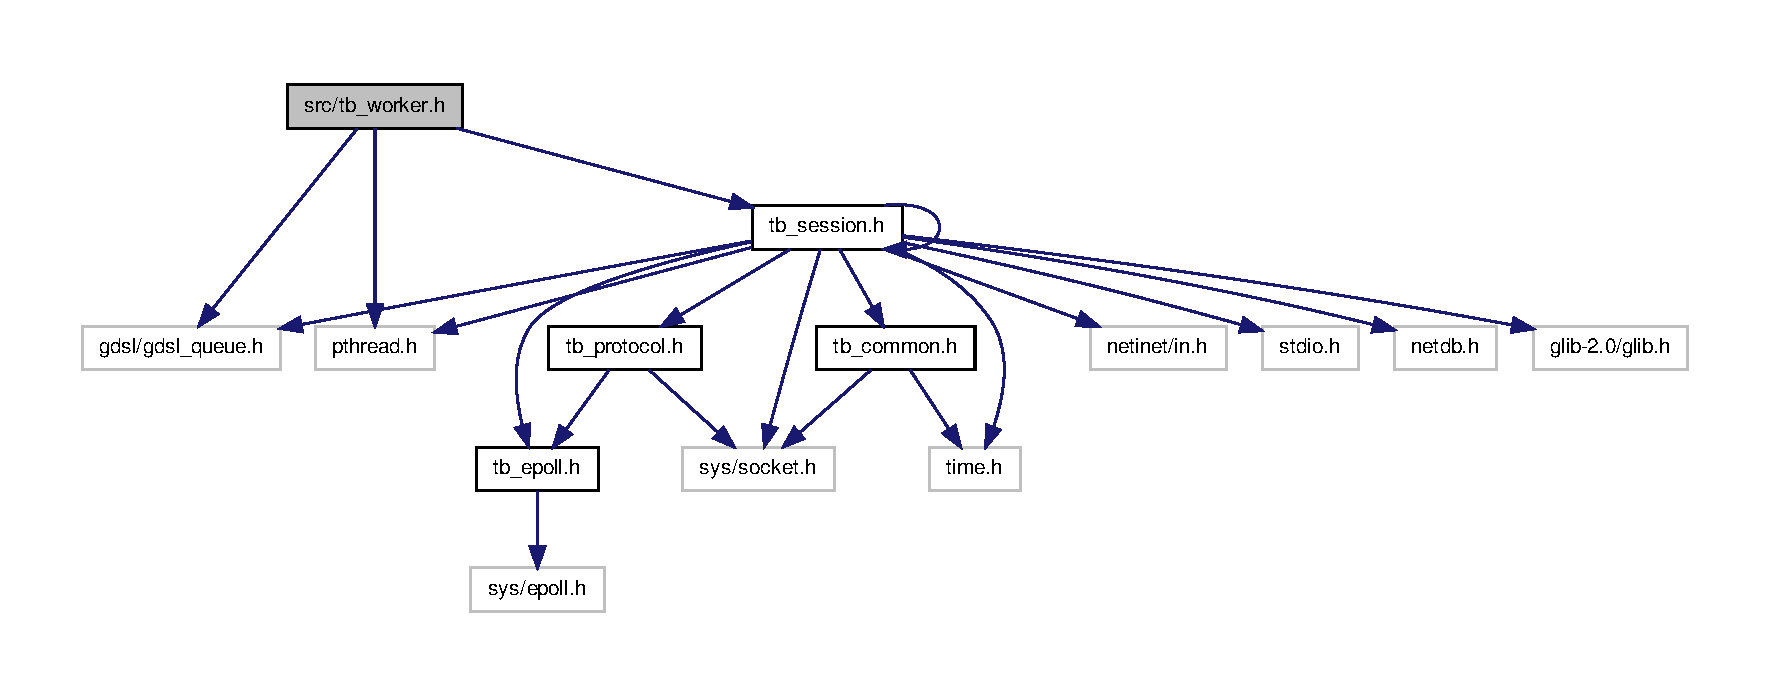
\includegraphics[width=350pt]{tb__worker_8h__incl}
\end{center}
\end{figure}
This graph shows which files directly or indirectly include this file\-:\nopagebreak
\begin{figure}[H]
\begin{center}
\leavevmode
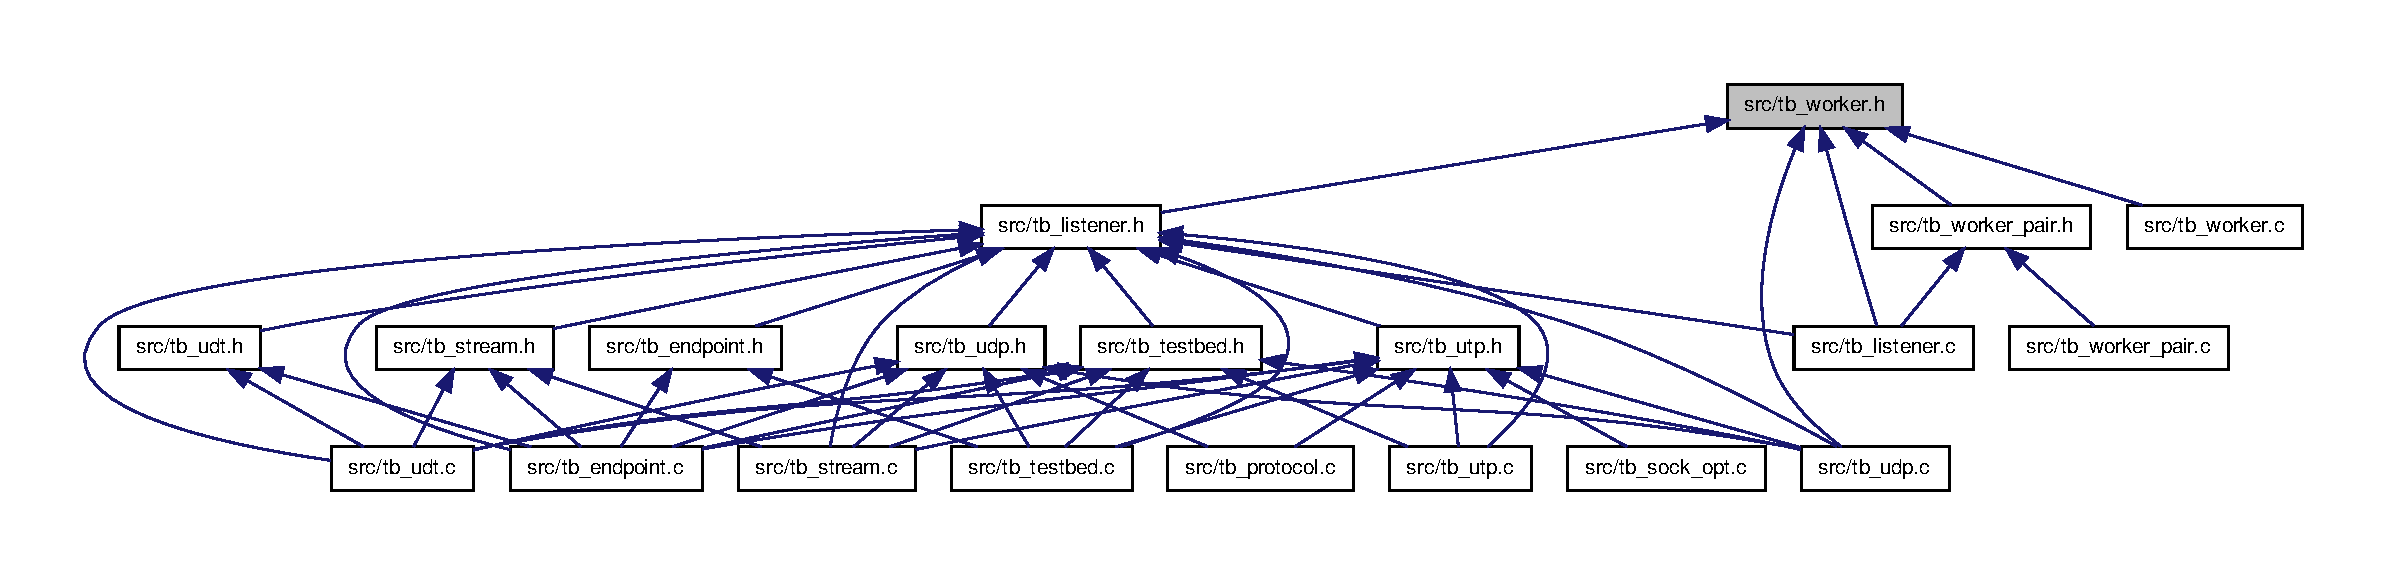
\includegraphics[width=350pt]{tb__worker_8h__dep__incl}
\end{center}
\end{figure}
\subsection*{Data Structures}
\begin{DoxyCompactItemize}
\item 
struct \hyperlink{structtb__worker__t}{tb\-\_\-worker\-\_\-t}
\begin{DoxyCompactList}\small\item\em struct that defines fields for worker. \end{DoxyCompactList}\end{DoxyCompactItemize}
\subsection*{Functions}
\begin{DoxyCompactItemize}
\item 
void $\ast$ \hyperlink{tb__worker_8h_afc515f36e24829670510abc9d736f921}{do\-\_\-work} (void $\ast$worker)
\begin{DoxyCompactList}\small\item\em Start work. \end{DoxyCompactList}\item 
void \hyperlink{tb__worker_8h_aa7815ec198375441b2d6dad28f0c6fce}{destroy\-\_\-worker} (\hyperlink{structtb__worker__t}{tb\-\_\-worker\-\_\-t} $\ast$w)
\begin{DoxyCompactList}\small\item\em Destroy the given worker, freeing memory. \end{DoxyCompactList}\item 
\hyperlink{structtb__worker__t}{tb\-\_\-worker\-\_\-t} $\ast$ \hyperlink{tb__worker_8h_a10a515d12c8fb7885a5cd5d1a67141fc}{create\-\_\-worker} ()
\begin{DoxyCompactList}\small\item\em Create a new worker, allocating memory as required. \end{DoxyCompactList}\item 
long int \hyperlink{tb__worker_8h_a8746fc48b8ce47ad0bdc8b521f7708d0}{compare\-\_\-workers} (gdsl\-\_\-element\-\_\-t E, void $\ast$value)
\begin{DoxyCompactList}\small\item\em Compare two workers, required by gdsl\-\_\-heap. \end{DoxyCompactList}\item 
\hyperlink{structtb__session__t}{tb\-\_\-session\-\_\-t} $\ast$ \hyperlink{tb__worker_8h_aceb05b8d10c44e2979cc78b5bde1b369}{get\-\_\-work} (\hyperlink{structtb__worker__t}{tb\-\_\-worker\-\_\-t} $\ast$worker)
\begin{DoxyCompactList}\small\item\em Get work for this worker. \end{DoxyCompactList}\item 
void \hyperlink{tb__worker_8h_aa5ef220c5813db06b41fccbf885a5727}{add\-\_\-work} (\hyperlink{structtb__worker__t}{tb\-\_\-worker\-\_\-t} $\ast$worker, \hyperlink{structtb__session__t}{tb\-\_\-session\-\_\-t} $\ast$data)
\begin{DoxyCompactList}\small\item\em Add work to a worker. \end{DoxyCompactList}\end{DoxyCompactItemize}


\subsection{Function Documentation}
\hypertarget{tb__worker_8h_aa5ef220c5813db06b41fccbf885a5727}{\index{tb\-\_\-worker.\-h@{tb\-\_\-worker.\-h}!add\-\_\-work@{add\-\_\-work}}
\index{add\-\_\-work@{add\-\_\-work}!tb_worker.h@{tb\-\_\-worker.\-h}}
\subsubsection[{add\-\_\-work}]{\setlength{\rightskip}{0pt plus 5cm}void add\-\_\-work (
\begin{DoxyParamCaption}
\item[{{\bf tb\-\_\-worker\-\_\-t} $\ast$}]{worker, }
\item[{{\bf tb\-\_\-session\-\_\-t} $\ast$}]{data}
\end{DoxyParamCaption}
)}}\label{tb__worker_8h_aa5ef220c5813db06b41fccbf885a5727}


Add work to a worker. 

Add work to the given worker. Is thread-\/safe, so it will block if another thread is adding work to the queue. The work is added to the work queue in the given worker.

\begin{DoxyPrecond}{Precondition}
worker must be of struct type \hyperlink{structtb__worker__t}{tb\-\_\-worker\-\_\-t}. 

data must be of type \hyperlink{structtb__session__t}{tb\-\_\-session\-\_\-t}.  parameters can be N\-U\-L\-L. 
\end{DoxyPrecond}

\begin{DoxyParams}{Parameters}
{\em worker} & The worker to add work to. \\
\hline
{\em data} & The work to be added. \\
\hline
\end{DoxyParams}
\begin{DoxyReturn}{Returns}
void 
\end{DoxyReturn}


Definition at line 72 of file tb\-\_\-worker.\-c.

\hypertarget{tb__worker_8h_a8746fc48b8ce47ad0bdc8b521f7708d0}{\index{tb\-\_\-worker.\-h@{tb\-\_\-worker.\-h}!compare\-\_\-workers@{compare\-\_\-workers}}
\index{compare\-\_\-workers@{compare\-\_\-workers}!tb_worker.h@{tb\-\_\-worker.\-h}}
\subsubsection[{compare\-\_\-workers}]{\setlength{\rightskip}{0pt plus 5cm}long int compare\-\_\-workers (
\begin{DoxyParamCaption}
\item[{gdsl\-\_\-element\-\_\-t}]{E, }
\item[{void $\ast$}]{value}
\end{DoxyParamCaption}
)}}\label{tb__worker_8h_a8746fc48b8ce47ad0bdc8b521f7708d0}


Compare two workers, required by gdsl\-\_\-heap. 

gdsl\-\_\-heap\-\_\-t is a max heap, so workers with a lesser number of tasks will return $>$ 0, same number of tasks = 0, and greater number of tasks $<$ 0.

\begin{DoxyPrecond}{Precondition}
E and value must be both of struct type worker. 

E and value cannot be N\-U\-L\-L. 
\end{DoxyPrecond}

\begin{DoxyParams}{Parameters}
{\em E} & The element to compare. \\
\hline
{\em value} & The element to compare against. \\
\hline
\end{DoxyParams}
\begin{DoxyReturn}{Returns}
-\/1, 0 and 1 if E is greater, equal, or less than. 
\end{DoxyReturn}


Definition at line 109 of file tb\-\_\-worker.\-c.

\hypertarget{tb__worker_8h_a10a515d12c8fb7885a5cd5d1a67141fc}{\index{tb\-\_\-worker.\-h@{tb\-\_\-worker.\-h}!create\-\_\-worker@{create\-\_\-worker}}
\index{create\-\_\-worker@{create\-\_\-worker}!tb_worker.h@{tb\-\_\-worker.\-h}}
\subsubsection[{create\-\_\-worker}]{\setlength{\rightskip}{0pt plus 5cm}{\bf tb\-\_\-worker\-\_\-t}$\ast$ create\-\_\-worker (
\begin{DoxyParamCaption}
{}
\end{DoxyParamCaption}
)}}\label{tb__worker_8h_a10a515d12c8fb7885a5cd5d1a67141fc}


Create a new worker, allocating memory as required. 

\begin{DoxyNote}{Note}
Each worker gets a new, unique id that is generated at the time of creation 
\end{DoxyNote}
\begin{DoxyReturn}{Returns}
worker$\ast$ Pointer to new \hyperlink{structtb__worker__t}{tb\-\_\-worker\-\_\-t}. 
\end{DoxyReturn}


Definition at line 44 of file tb\-\_\-worker.\-c.

\hypertarget{tb__worker_8h_aa7815ec198375441b2d6dad28f0c6fce}{\index{tb\-\_\-worker.\-h@{tb\-\_\-worker.\-h}!destroy\-\_\-worker@{destroy\-\_\-worker}}
\index{destroy\-\_\-worker@{destroy\-\_\-worker}!tb_worker.h@{tb\-\_\-worker.\-h}}
\subsubsection[{destroy\-\_\-worker}]{\setlength{\rightskip}{0pt plus 5cm}void destroy\-\_\-worker (
\begin{DoxyParamCaption}
\item[{{\bf tb\-\_\-worker\-\_\-t} $\ast$}]{w}
\end{DoxyParamCaption}
)}}\label{tb__worker_8h_aa7815ec198375441b2d6dad28f0c6fce}


Destroy the given worker, freeing memory. 

\begin{DoxyNote}{Note}

\end{DoxyNote}
\begin{DoxyPrecond}{Precondition}
w must be of struct type worker. 
\end{DoxyPrecond}

\begin{DoxyParams}{Parameters}
{\em w} & The worker to destroy \\
\hline
\end{DoxyParams}


Definition at line 61 of file tb\-\_\-worker.\-c.

\hypertarget{tb__worker_8h_afc515f36e24829670510abc9d736f921}{\index{tb\-\_\-worker.\-h@{tb\-\_\-worker.\-h}!do\-\_\-work@{do\-\_\-work}}
\index{do\-\_\-work@{do\-\_\-work}!tb_worker.h@{tb\-\_\-worker.\-h}}
\subsubsection[{do\-\_\-work}]{\setlength{\rightskip}{0pt plus 5cm}void$\ast$ do\-\_\-work (
\begin{DoxyParamCaption}
\item[{void $\ast$}]{worker}
\end{DoxyParamCaption}
)}}\label{tb__worker_8h_afc515f36e24829670510abc9d736f921}


Start work. 

This is the function that is passed to pthread\-\_\-create. The worker struct is passed in by pthread\-\_\-create as per the api

\begin{DoxySeeAlso}{See Also}
pthread.\-h 

pthread\-\_\-create 
\end{DoxySeeAlso}
\begin{DoxyPrecond}{Precondition}
param Must be of struct type worker, cannot be N\-U\-L\-L. 
\end{DoxyPrecond}

\begin{DoxyParams}{Parameters}
{\em worker} & The worker to do the specified work. \\
\hline
\end{DoxyParams}
\begin{DoxyReturn}{Returns}
void 
\end{DoxyReturn}


Definition at line 25 of file tb\-\_\-worker.\-c.

\hypertarget{tb__worker_8h_aceb05b8d10c44e2979cc78b5bde1b369}{\index{tb\-\_\-worker.\-h@{tb\-\_\-worker.\-h}!get\-\_\-work@{get\-\_\-work}}
\index{get\-\_\-work@{get\-\_\-work}!tb_worker.h@{tb\-\_\-worker.\-h}}
\subsubsection[{get\-\_\-work}]{\setlength{\rightskip}{0pt plus 5cm}{\bf tb\-\_\-session\-\_\-t}$\ast$ get\-\_\-work (
\begin{DoxyParamCaption}
\item[{{\bf tb\-\_\-worker\-\_\-t} $\ast$}]{worker}
\end{DoxyParamCaption}
)}}\label{tb__worker_8h_aceb05b8d10c44e2979cc78b5bde1b369}


Get work for this worker. 

Gets a unit of work for this worker. Blocks if the queue is empty.

\begin{DoxyPrecond}{Precondition}
worker must be of struct type worker. 

worker cannot be N\-U\-L\-L 
\end{DoxyPrecond}

\begin{DoxyParams}{Parameters}
{\em worker} & The worker to fetch the work for. \\
\hline
\end{DoxyParams}
\begin{DoxyReturn}{Returns}
Work to be done by this \hyperlink{structtb__worker__t}{tb\-\_\-worker\-\_\-t}. 
\end{DoxyReturn}


Definition at line 86 of file tb\-\_\-worker.\-c.


\hypertarget{tb__worker__pair_8c}{\section{src/tb\-\_\-worker\-\_\-pair.c File Reference}
\label{tb__worker__pair_8c}\index{src/tb\-\_\-worker\-\_\-pair.\-c@{src/tb\-\_\-worker\-\_\-pair.\-c}}
}
{\ttfamily \#include \char`\"{}tb\-\_\-worker\-\_\-pair.\-h\char`\"{}}\\*
{\ttfamily \#include $<$stdlib.\-h$>$}\\*
{\ttfamily \#include $<$string.\-h$>$}\\*
{\ttfamily \#include $<$gdsl.\-h$>$}\\*
Include dependency graph for tb\-\_\-worker\-\_\-pair.\-c\-:\nopagebreak
\begin{figure}[H]
\begin{center}
\leavevmode
\includegraphics[width=350pt]{tb__worker__pair_8c__incl}
\end{center}
\end{figure}
\subsection*{Functions}
\begin{DoxyCompactItemize}
\item 
char $\ast$ \hyperlink{tb__worker__pair_8c_a62336f06f995e4ebc04e178ede39ec2d}{get\-\_\-pair\-\_\-key} (void $\ast$data)
\item 
gdsl\-\_\-element\-\_\-t $\ast$ \hyperlink{tb__worker__pair_8c_a715a32c83662eea0cb1f4f8f113bd3e0}{allocate\-\_\-tuple} (void $\ast$data)
\item 
void \hyperlink{tb__worker__pair_8c_a2064cc380d479674048dde60091b390c}{free\-\_\-tuple} (gdsl\-\_\-element\-\_\-t $\ast$data)
\end{DoxyCompactItemize}


\subsection{Function Documentation}
\hypertarget{tb__worker__pair_8c_a715a32c83662eea0cb1f4f8f113bd3e0}{\index{tb\-\_\-worker\-\_\-pair.\-c@{tb\-\_\-worker\-\_\-pair.\-c}!allocate\-\_\-tuple@{allocate\-\_\-tuple}}
\index{allocate\-\_\-tuple@{allocate\-\_\-tuple}!tb_worker_pair.c@{tb\-\_\-worker\-\_\-pair.\-c}}
\subsubsection[{allocate\-\_\-tuple}]{\setlength{\rightskip}{0pt plus 5cm}gdsl\-\_\-element\-\_\-t$\ast$ allocate\-\_\-tuple (
\begin{DoxyParamCaption}
\item[{void $\ast$}]{data}
\end{DoxyParamCaption}
)}}\label{tb__worker__pair_8c_a715a32c83662eea0cb1f4f8f113bd3e0}


Definition at line 21 of file tb\-\_\-worker\-\_\-pair.\-c.

\hypertarget{tb__worker__pair_8c_a2064cc380d479674048dde60091b390c}{\index{tb\-\_\-worker\-\_\-pair.\-c@{tb\-\_\-worker\-\_\-pair.\-c}!free\-\_\-tuple@{free\-\_\-tuple}}
\index{free\-\_\-tuple@{free\-\_\-tuple}!tb_worker_pair.c@{tb\-\_\-worker\-\_\-pair.\-c}}
\subsubsection[{free\-\_\-tuple}]{\setlength{\rightskip}{0pt plus 5cm}void free\-\_\-tuple (
\begin{DoxyParamCaption}
\item[{gdsl\-\_\-element\-\_\-t $\ast$}]{data}
\end{DoxyParamCaption}
)}}\label{tb__worker__pair_8c_a2064cc380d479674048dde60091b390c}


Definition at line 30 of file tb\-\_\-worker\-\_\-pair.\-c.

\hypertarget{tb__worker__pair_8c_a62336f06f995e4ebc04e178ede39ec2d}{\index{tb\-\_\-worker\-\_\-pair.\-c@{tb\-\_\-worker\-\_\-pair.\-c}!get\-\_\-pair\-\_\-key@{get\-\_\-pair\-\_\-key}}
\index{get\-\_\-pair\-\_\-key@{get\-\_\-pair\-\_\-key}!tb_worker_pair.c@{tb\-\_\-worker\-\_\-pair.\-c}}
\subsubsection[{get\-\_\-pair\-\_\-key}]{\setlength{\rightskip}{0pt plus 5cm}char$\ast$ get\-\_\-pair\-\_\-key (
\begin{DoxyParamCaption}
\item[{void $\ast$}]{data}
\end{DoxyParamCaption}
)}}\label{tb__worker__pair_8c_a62336f06f995e4ebc04e178ede39ec2d}


Definition at line 14 of file tb\-\_\-worker\-\_\-pair.\-c.


\hypertarget{tb__worker__pair_8h}{\section{src/tb\-\_\-worker\-\_\-pair.h File Reference}
\label{tb__worker__pair_8h}\index{src/tb\-\_\-worker\-\_\-pair.\-h@{src/tb\-\_\-worker\-\_\-pair.\-h}}
}
{\ttfamily \#include \char`\"{}tb\-\_\-worker.\-h\char`\"{}}\\*
{\ttfamily \#include \char`\"{}tb\-\_\-session.\-h\char`\"{}}\\*
{\ttfamily \#include $<$gdsl/gdsl\-\_\-hash.\-h$>$}\\*
Include dependency graph for tb\-\_\-worker\-\_\-pair.\-h\-:\nopagebreak
\begin{figure}[H]
\begin{center}
\leavevmode
\includegraphics[width=350pt]{tb__worker__pair_8h__incl}
\end{center}
\end{figure}
This graph shows which files directly or indirectly include this file\-:\nopagebreak
\begin{figure}[H]
\begin{center}
\leavevmode
\includegraphics[width=288pt]{tb__worker__pair_8h__dep__incl}
\end{center}
\end{figure}
\subsection*{Data Structures}
\begin{DoxyCompactItemize}
\item 
struct \hyperlink{structtb__worker__pair__t}{tb\-\_\-worker\-\_\-pair\-\_\-t}
\end{DoxyCompactItemize}
\subsection*{Functions}
\begin{DoxyCompactItemize}
\item 
char $\ast$ \hyperlink{tb__worker__pair_8h_a62336f06f995e4ebc04e178ede39ec2d}{get\-\_\-pair\-\_\-key} (void $\ast$data)
\item 
gdsl\-\_\-element\-\_\-t $\ast$ \hyperlink{tb__worker__pair_8h_a715a32c83662eea0cb1f4f8f113bd3e0}{allocate\-\_\-tuple} (void $\ast$data)
\item 
void \hyperlink{tb__worker__pair_8h_a2064cc380d479674048dde60091b390c}{free\-\_\-tuple} (gdsl\-\_\-element\-\_\-t $\ast$data)
\end{DoxyCompactItemize}


\subsection{Function Documentation}
\hypertarget{tb__worker__pair_8h_a715a32c83662eea0cb1f4f8f113bd3e0}{\index{tb\-\_\-worker\-\_\-pair.\-h@{tb\-\_\-worker\-\_\-pair.\-h}!allocate\-\_\-tuple@{allocate\-\_\-tuple}}
\index{allocate\-\_\-tuple@{allocate\-\_\-tuple}!tb_worker_pair.h@{tb\-\_\-worker\-\_\-pair.\-h}}
\subsubsection[{allocate\-\_\-tuple}]{\setlength{\rightskip}{0pt plus 5cm}gdsl\-\_\-element\-\_\-t$\ast$ allocate\-\_\-tuple (
\begin{DoxyParamCaption}
\item[{void $\ast$}]{data}
\end{DoxyParamCaption}
)}}\label{tb__worker__pair_8h_a715a32c83662eea0cb1f4f8f113bd3e0}


Definition at line 21 of file tb\-\_\-worker\-\_\-pair.\-c.

\hypertarget{tb__worker__pair_8h_a2064cc380d479674048dde60091b390c}{\index{tb\-\_\-worker\-\_\-pair.\-h@{tb\-\_\-worker\-\_\-pair.\-h}!free\-\_\-tuple@{free\-\_\-tuple}}
\index{free\-\_\-tuple@{free\-\_\-tuple}!tb_worker_pair.h@{tb\-\_\-worker\-\_\-pair.\-h}}
\subsubsection[{free\-\_\-tuple}]{\setlength{\rightskip}{0pt plus 5cm}void free\-\_\-tuple (
\begin{DoxyParamCaption}
\item[{gdsl\-\_\-element\-\_\-t $\ast$}]{data}
\end{DoxyParamCaption}
)}}\label{tb__worker__pair_8h_a2064cc380d479674048dde60091b390c}


Definition at line 30 of file tb\-\_\-worker\-\_\-pair.\-c.

\hypertarget{tb__worker__pair_8h_a62336f06f995e4ebc04e178ede39ec2d}{\index{tb\-\_\-worker\-\_\-pair.\-h@{tb\-\_\-worker\-\_\-pair.\-h}!get\-\_\-pair\-\_\-key@{get\-\_\-pair\-\_\-key}}
\index{get\-\_\-pair\-\_\-key@{get\-\_\-pair\-\_\-key}!tb_worker_pair.h@{tb\-\_\-worker\-\_\-pair.\-h}}
\subsubsection[{get\-\_\-pair\-\_\-key}]{\setlength{\rightskip}{0pt plus 5cm}char$\ast$ get\-\_\-pair\-\_\-key (
\begin{DoxyParamCaption}
\item[{void $\ast$}]{data}
\end{DoxyParamCaption}
)}}\label{tb__worker__pair_8h_a62336f06f995e4ebc04e178ede39ec2d}


Definition at line 14 of file tb\-\_\-worker\-\_\-pair.\-c.


\printindex
\end{document}
